\documentclass[english]{scrartcl}
\usepackage[osf]{mathpazo}
\usepackage[utf8]{inputenc}
\usepackage[T1]{fontenc}
\usepackage{babel}
\usepackage[usenames,dvipsnames]{color}
\usepackage{tikz}
\usepackage{gnuplot-lua-tikz}
\usepackage{amsmath,amssymb}
\usepackage{caption}
\usepackage{listings}
\usepackage{booktabs}
\lstset{language=xml,numbers=left,stepnumber=5,numberstyle=\ttfamily\color{Purple},basicstyle=\small\ttfamily,keywordstyle=\itshape,stringstyle=\color{Bittersweet},morekeywords={Expression,Function,Parameter,VectorField,StateVariable}}

\setcapindent{0em}
\addtokomafont{captionlabel}{\bfseries}
\addtokomafont{title}{\rmfamily}

\author{Andrei Kramer}
\title{Analysis of a large Sample}
\subject{MCMC\_CLIB}

\begin{document}
\maketitle
\begin{center}
  \hspace*{-1cm}
  % GNUPLOT: LaTeX picture with Postscript
\begingroup
  \makeatletter
  \providecommand\color[2][]{%
    \GenericError{(gnuplot) \space\space\space\@spaces}{%
      Package color not loaded in conjunction with
      terminal option `colourtext'%
    }{See the gnuplot documentation for explanation.%
    }{Either use 'blacktext' in gnuplot or load the package
      color.sty in LaTeX.}%
    \renewcommand\color[2][]{}%
  }%
  \providecommand\includegraphics[2][]{%
    \GenericError{(gnuplot) \space\space\space\@spaces}{%
      Package graphicx or graphics not loaded%
    }{See the gnuplot documentation for explanation.%
    }{The gnuplot epslatex terminal needs graphicx.sty or graphics.sty.}%
    \renewcommand\includegraphics[2][]{}%
  }%
  \providecommand\rotatebox[2]{#2}%
  \@ifundefined{ifGPcolor}{%
    \newif\ifGPcolor
    \GPcolorfalse
  }{}%
  \@ifundefined{ifGPblacktext}{%
    \newif\ifGPblacktext
    \GPblacktexttrue
  }{}%
  % define a \g@addto@macro without @ in the name:
  \let\gplgaddtomacro\g@addto@macro
  % define empty templates for all commands taking text:
  \gdef\gplbacktext{}%
  \gdef\gplfronttext{}%
  \makeatother
  \ifGPblacktext
    % no textcolor at all
    \def\colorrgb#1{}%
    \def\colorgray#1{}%
  \else
    % gray or color?
    \ifGPcolor
      \def\colorrgb#1{\color[rgb]{#1}}%
      \def\colorgray#1{\color[gray]{#1}}%
      \expandafter\def\csname LTw\endcsname{\color{white}}%
      \expandafter\def\csname LTb\endcsname{\color{black}}%
      \expandafter\def\csname LTa\endcsname{\color{black}}%
      \expandafter\def\csname LT0\endcsname{\color[rgb]{1,0,0}}%
      \expandafter\def\csname LT1\endcsname{\color[rgb]{0,1,0}}%
      \expandafter\def\csname LT2\endcsname{\color[rgb]{0,0,1}}%
      \expandafter\def\csname LT3\endcsname{\color[rgb]{1,0,1}}%
      \expandafter\def\csname LT4\endcsname{\color[rgb]{0,1,1}}%
      \expandafter\def\csname LT5\endcsname{\color[rgb]{1,1,0}}%
      \expandafter\def\csname LT6\endcsname{\color[rgb]{0,0,0}}%
      \expandafter\def\csname LT7\endcsname{\color[rgb]{1,0.3,0}}%
      \expandafter\def\csname LT8\endcsname{\color[rgb]{0.5,0.5,0.5}}%
    \else
      % gray
      \def\colorrgb#1{\color{black}}%
      \def\colorgray#1{\color[gray]{#1}}%
      \expandafter\def\csname LTw\endcsname{\color{white}}%
      \expandafter\def\csname LTb\endcsname{\color{black}}%
      \expandafter\def\csname LTa\endcsname{\color{black}}%
      \expandafter\def\csname LT0\endcsname{\color{black}}%
      \expandafter\def\csname LT1\endcsname{\color{black}}%
      \expandafter\def\csname LT2\endcsname{\color{black}}%
      \expandafter\def\csname LT3\endcsname{\color{black}}%
      \expandafter\def\csname LT4\endcsname{\color{black}}%
      \expandafter\def\csname LT5\endcsname{\color{black}}%
      \expandafter\def\csname LT6\endcsname{\color{black}}%
      \expandafter\def\csname LT7\endcsname{\color{black}}%
      \expandafter\def\csname LT8\endcsname{\color{black}}%
    \fi
  \fi
  \setlength{\unitlength}{0.0500bp}%
  \begin{picture}(9070.00,5668.00)%
    \gplgaddtomacro\gplbacktext{%
      \colorrgb{0.00,0.00,0.00}%
      \put(740,760){\makebox(0,0)[r]{\strut{}-10}}%
      \colorrgb{0.00,0.00,0.00}%
      \put(740,1644){\makebox(0,0)[r]{\strut{}-5}}%
      \colorrgb{0.00,0.00,0.00}%
      \put(740,2529){\makebox(0,0)[r]{\strut{}0}}%
      \colorrgb{0.00,0.00,0.00}%
      \put(740,3413){\makebox(0,0)[r]{\strut{}5}}%
      \colorrgb{0.00,0.00,0.00}%
      \put(740,4297){\makebox(0,0)[r]{\strut{}10}}%
      \colorrgb{0.00,0.00,0.00}%
      \put(740,5181){\makebox(0,0)[r]{\strut{}15}}%
      \colorrgb{0.00,0.00,0.00}%
      \put(2158,440){\makebox(0,0){\strut{}5}}%
      \colorrgb{0.00,0.00,0.00}%
      \put(3703,440){\makebox(0,0){\strut{}10}}%
      \colorrgb{0.00,0.00,0.00}%
      \put(5248,440){\makebox(0,0){\strut{}15}}%
      \colorrgb{0.00,0.00,0.00}%
      \put(6793,440){\makebox(0,0){\strut{}20}}%
      \colorrgb{0.00,0.00,0.00}%
      \put(8338,440){\makebox(0,0){\strut{}25}}%
      \colorrgb{0.00,0.00,0.00}%
      \put(160,3033){\rotatebox{90}{\makebox(0,0){\strut{}$\theta_i$}}}%
      \colorrgb{0.00,0.00,0.00}%
      \put(4784,140){\makebox(0,0){\strut{}$i$}}%
    }%
    \gplgaddtomacro\gplfronttext{%
      \csname LTb\endcsname%
      \put(7806,5264){\makebox(0,0)[r]{\strut{}mean}}%
    }%
    \gplbacktext
    \put(0,0){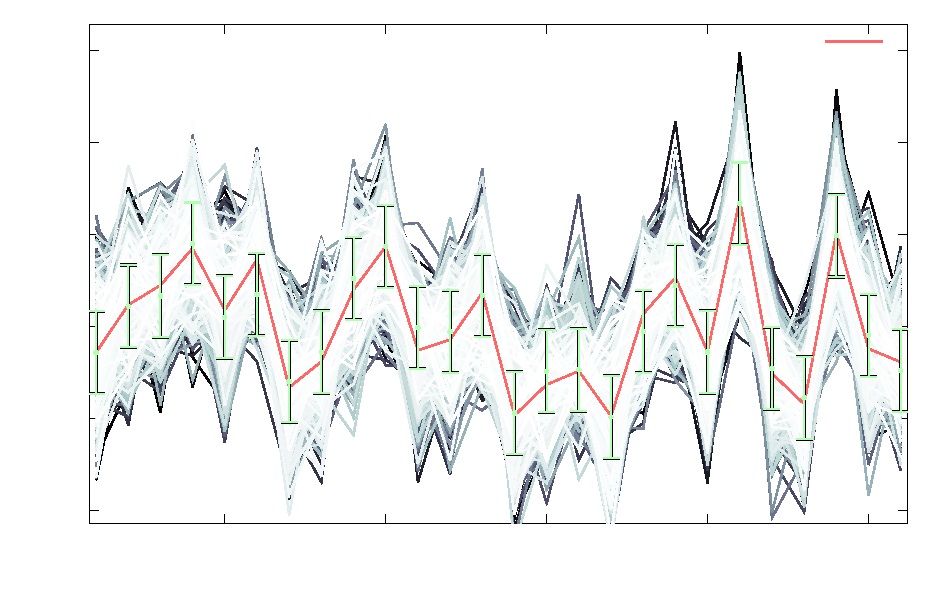
\includegraphics{sample}}%
    \gplfronttext
  \end{picture}%
\endgroup

  \captionof{figure}{The Posterior Sample of size $N=1\times10^6$, as
    obtained from the \texttt{MCMC\_CLIB}; thinned out using the
    integrated autocorrelation length $\tau_{\text{int.},l}=1516(250)$
    (estimated using the log-posterior $l$ as observable). The red
    line indicates the maximum posterior estimate, while the green
    errorbars indicate the used prior distribution
    (Gaussian).\label{fig:pc-sample}}
\end{center}

The sample was obtained in $t_{\text{s}}=267385$\,s. Considering the
auto-correlation, the effective sampling speed is:
\begin{equation}
  \label{eq:speed}
  v=\frac{N}{2\tau_{\text{int.},l} t_{\text{s}}}=12(2)\times 10^{-4}\,\text{s}^{-1}\,.
\end{equation}
\begin{center}
  \sffamily\tiny
  \hspace*{-3cm}
  \begin{tikzpicture}
    \node (plot) {% GNUPLOT: LaTeX picture with Postscript
\begingroup
  \makeatletter
  \providecommand\color[2][]{%
    \GenericError{(gnuplot) \space\space\space\@spaces}{%
      Package color not loaded in conjunction with
      terminal option `colourtext'%
    }{See the gnuplot documentation for explanation.%
    }{Either use 'blacktext' in gnuplot or load the package
      color.sty in LaTeX.}%
    \renewcommand\color[2][]{}%
  }%
  \providecommand\includegraphics[2][]{%
    \GenericError{(gnuplot) \space\space\space\@spaces}{%
      Package graphicx or graphics not loaded%
    }{See the gnuplot documentation for explanation.%
    }{The gnuplot epslatex terminal needs graphicx.sty or graphics.sty.}%
    \renewcommand\includegraphics[2][]{}%
  }%
  \providecommand\rotatebox[2]{#2}%
  \@ifundefined{ifGPcolor}{%
    \newif\ifGPcolor
    \GPcolorfalse
  }{}%
  \@ifundefined{ifGPblacktext}{%
    \newif\ifGPblacktext
    \GPblacktexttrue
  }{}%
  % define a \g@addto@macro without @ in the name:
  \let\gplgaddtomacro\g@addto@macro
  % define empty templates for all commands taking text:
  \gdef\gplbacktext{}%
  \gdef\gplfronttext{}%
  \makeatother
  \ifGPblacktext
    % no textcolor at all
    \def\colorrgb#1{}%
    \def\colorgray#1{}%
  \else
    % gray or color?
    \ifGPcolor
      \def\colorrgb#1{\color[rgb]{#1}}%
      \def\colorgray#1{\color[gray]{#1}}%
      \expandafter\def\csname LTw\endcsname{\color{white}}%
      \expandafter\def\csname LTb\endcsname{\color{black}}%
      \expandafter\def\csname LTa\endcsname{\color{black}}%
      \expandafter\def\csname LT0\endcsname{\color[rgb]{1,0,0}}%
      \expandafter\def\csname LT1\endcsname{\color[rgb]{0,1,0}}%
      \expandafter\def\csname LT2\endcsname{\color[rgb]{0,0,1}}%
      \expandafter\def\csname LT3\endcsname{\color[rgb]{1,0,1}}%
      \expandafter\def\csname LT4\endcsname{\color[rgb]{0,1,1}}%
      \expandafter\def\csname LT5\endcsname{\color[rgb]{1,1,0}}%
      \expandafter\def\csname LT6\endcsname{\color[rgb]{0,0,0}}%
      \expandafter\def\csname LT7\endcsname{\color[rgb]{1,0.3,0}}%
      \expandafter\def\csname LT8\endcsname{\color[rgb]{0.5,0.5,0.5}}%
    \else
      % gray
      \def\colorrgb#1{\color{black}}%
      \def\colorgray#1{\color[gray]{#1}}%
      \expandafter\def\csname LTw\endcsname{\color{white}}%
      \expandafter\def\csname LTb\endcsname{\color{black}}%
      \expandafter\def\csname LTa\endcsname{\color{black}}%
      \expandafter\def\csname LT0\endcsname{\color{black}}%
      \expandafter\def\csname LT1\endcsname{\color{black}}%
      \expandafter\def\csname LT2\endcsname{\color{black}}%
      \expandafter\def\csname LT3\endcsname{\color{black}}%
      \expandafter\def\csname LT4\endcsname{\color{black}}%
      \expandafter\def\csname LT5\endcsname{\color{black}}%
      \expandafter\def\csname LT6\endcsname{\color{black}}%
      \expandafter\def\csname LT7\endcsname{\color{black}}%
      \expandafter\def\csname LT8\endcsname{\color{black}}%
    \fi
  \fi
  \setlength{\unitlength}{0.0500bp}%
  \begin{picture}(11520.00,8640.00)%
    \gplgaddtomacro\gplbacktext{%
      \colorrgb{0.00,0.00,0.00}%
      \put(1377,6629){\makebox(0,0)[r]{\strut{}0}}%
      \colorrgb{0.00,0.00,0.00}%
      \put(1377,6856){\makebox(0,0)[r]{\strut{}1}}%
      \colorrgb{0.00,0.00,0.00}%
      \put(1377,7084){\makebox(0,0)[r]{\strut{}2}}%
      \colorrgb{0.00,0.00,0.00}%
      \put(1377,7311){\makebox(0,0)[r]{\strut{}3}}%
      \colorrgb{0.00,0.00,0.00}%
      \put(1377,7538){\makebox(0,0)[r]{\strut{}4}}%
      \colorrgb{0.00,0.00,0.00}%
      \put(1377,7766){\makebox(0,0)[r]{\strut{}5}}%
      \colorrgb{0.00,0.00,0.00}%
      \put(1377,7993){\makebox(0,0)[r]{\strut{}6}}%
      \colorrgb{0.00,0.00,0.00}%
      \put(2087,6429){\makebox(0,0){\strut{}.1}}%
      \colorrgb{0.00,0.00,0.00}%
      \put(2145,6429){\makebox(0,0){\strut{}8}}%
      \colorrgb{0.00,0.00,0.00}%
      \put(2264,6429){\makebox(0,0){\strut{}24}}%
      \colorrgb{0.00,0.00,0.00}%
      \put(2443,6429){\makebox(0,0){\strut{}48}}%
      \colorrgb{0.00,0.00,0.00}%
      \put(2621,6429){\makebox(0,0){\strut{}72}}%
    }%
    \gplgaddtomacro\gplfronttext{%
    }%
    \gplgaddtomacro\gplbacktext{%
      \colorrgb{0.00,0.00,0.00}%
      \put(2927,6629){\makebox(0,0)[r]{\strut{}0}}%
      \colorrgb{0.00,0.00,0.00}%
      \put(2927,6804){\makebox(0,0)[r]{\strut{}0.2}}%
      \colorrgb{0.00,0.00,0.00}%
      \put(2927,6979){\makebox(0,0)[r]{\strut{}0.4}}%
      \colorrgb{0.00,0.00,0.00}%
      \put(2927,7154){\makebox(0,0)[r]{\strut{}0.6}}%
      \colorrgb{0.00,0.00,0.00}%
      \put(2927,7328){\makebox(0,0)[r]{\strut{}0.8}}%
      \colorrgb{0.00,0.00,0.00}%
      \put(2927,7503){\makebox(0,0)[r]{\strut{}1}}%
      \colorrgb{0.00,0.00,0.00}%
      \put(2927,7678){\makebox(0,0)[r]{\strut{}1.2}}%
      \colorrgb{0.00,0.00,0.00}%
      \put(2927,7853){\makebox(0,0)[r]{\strut{}1.4}}%
      \colorrgb{0.00,0.00,0.00}%
      \put(3637,6429){\makebox(0,0){\strut{}.1}}%
      \colorrgb{0.00,0.00,0.00}%
      \put(3695,6429){\makebox(0,0){\strut{}8}}%
      \colorrgb{0.00,0.00,0.00}%
      \put(3814,6429){\makebox(0,0){\strut{}24}}%
      \colorrgb{0.00,0.00,0.00}%
      \put(3993,6429){\makebox(0,0){\strut{}48}}%
      \colorrgb{0.00,0.00,0.00}%
      \put(4171,6429){\makebox(0,0){\strut{}72}}%
    }%
    \gplgaddtomacro\gplfronttext{%
    }%
    \gplgaddtomacro\gplbacktext{%
      \colorrgb{0.00,0.00,0.00}%
      \put(4477,6629){\makebox(0,0)[r]{\strut{}0}}%
      \colorrgb{0.00,0.00,0.00}%
      \put(4477,6868){\makebox(0,0)[r]{\strut{}0.2}}%
      \colorrgb{0.00,0.00,0.00}%
      \put(4477,7107){\makebox(0,0)[r]{\strut{}0.4}}%
      \colorrgb{0.00,0.00,0.00}%
      \put(4477,7346){\makebox(0,0)[r]{\strut{}0.6}}%
      \colorrgb{0.00,0.00,0.00}%
      \put(4477,7585){\makebox(0,0)[r]{\strut{}0.8}}%
      \colorrgb{0.00,0.00,0.00}%
      \put(4477,7824){\makebox(0,0)[r]{\strut{}1}}%
      \colorrgb{0.00,0.00,0.00}%
      \put(5187,6429){\makebox(0,0){\strut{}.1}}%
      \colorrgb{0.00,0.00,0.00}%
      \put(5245,6429){\makebox(0,0){\strut{}8}}%
      \colorrgb{0.00,0.00,0.00}%
      \put(5364,6429){\makebox(0,0){\strut{}24}}%
      \colorrgb{0.00,0.00,0.00}%
      \put(5543,6429){\makebox(0,0){\strut{}48}}%
      \colorrgb{0.00,0.00,0.00}%
      \put(5721,6429){\makebox(0,0){\strut{}72}}%
    }%
    \gplgaddtomacro\gplfronttext{%
    }%
    \gplgaddtomacro\gplbacktext{%
      \colorrgb{0.00,0.00,0.00}%
      \put(6027,6629){\makebox(0,0)[r]{\strut{}0}}%
      \colorrgb{0.00,0.00,0.00}%
      \put(6027,6872){\makebox(0,0)[r]{\strut{}0.2}}%
      \colorrgb{0.00,0.00,0.00}%
      \put(6027,7114){\makebox(0,0)[r]{\strut{}0.4}}%
      \colorrgb{0.00,0.00,0.00}%
      \put(6027,7357){\makebox(0,0)[r]{\strut{}0.6}}%
      \colorrgb{0.00,0.00,0.00}%
      \put(6027,7599){\makebox(0,0)[r]{\strut{}0.8}}%
      \colorrgb{0.00,0.00,0.00}%
      \put(6027,7842){\makebox(0,0)[r]{\strut{}1}}%
      \colorrgb{0.00,0.00,0.00}%
      \put(6736,6429){\makebox(0,0){\strut{}.1}}%
      \colorrgb{0.00,0.00,0.00}%
      \put(6795,6429){\makebox(0,0){\strut{}8}}%
      \colorrgb{0.00,0.00,0.00}%
      \put(6914,6429){\makebox(0,0){\strut{}24}}%
      \colorrgb{0.00,0.00,0.00}%
      \put(7092,6429){\makebox(0,0){\strut{}48}}%
      \colorrgb{0.00,0.00,0.00}%
      \put(7271,6429){\makebox(0,0){\strut{}72}}%
    }%
    \gplgaddtomacro\gplfronttext{%
    }%
    \gplgaddtomacro\gplbacktext{%
      \colorrgb{0.00,0.00,0.00}%
      \put(7577,6629){\makebox(0,0)[r]{\strut{}0}}%
      \colorrgb{0.00,0.00,0.00}%
      \put(7577,6805){\makebox(0,0)[r]{\strut{}0.2}}%
      \colorrgb{0.00,0.00,0.00}%
      \put(7577,6982){\makebox(0,0)[r]{\strut{}0.4}}%
      \colorrgb{0.00,0.00,0.00}%
      \put(7577,7158){\makebox(0,0)[r]{\strut{}0.6}}%
      \colorrgb{0.00,0.00,0.00}%
      \put(7577,7335){\makebox(0,0)[r]{\strut{}0.8}}%
      \colorrgb{0.00,0.00,0.00}%
      \put(7577,7511){\makebox(0,0)[r]{\strut{}1}}%
      \colorrgb{0.00,0.00,0.00}%
      \put(7577,7688){\makebox(0,0)[r]{\strut{}1.2}}%
      \colorrgb{0.00,0.00,0.00}%
      \put(7577,7864){\makebox(0,0)[r]{\strut{}1.4}}%
      \colorrgb{0.00,0.00,0.00}%
      \put(8286,6429){\makebox(0,0){\strut{}.1}}%
      \colorrgb{0.00,0.00,0.00}%
      \put(8345,6429){\makebox(0,0){\strut{}8}}%
      \colorrgb{0.00,0.00,0.00}%
      \put(8464,6429){\makebox(0,0){\strut{}24}}%
      \colorrgb{0.00,0.00,0.00}%
      \put(8642,6429){\makebox(0,0){\strut{}48}}%
      \colorrgb{0.00,0.00,0.00}%
      \put(8821,6429){\makebox(0,0){\strut{}72}}%
    }%
    \gplgaddtomacro\gplfronttext{%
    }%
    \gplgaddtomacro\gplbacktext{%
      \colorrgb{0.00,0.00,0.00}%
      \put(9127,6629){\makebox(0,0)[r]{\strut{}0}}%
      \colorrgb{0.00,0.00,0.00}%
      \put(9127,6877){\makebox(0,0)[r]{\strut{}0.2}}%
      \colorrgb{0.00,0.00,0.00}%
      \put(9127,7124){\makebox(0,0)[r]{\strut{}0.4}}%
      \colorrgb{0.00,0.00,0.00}%
      \put(9127,7372){\makebox(0,0)[r]{\strut{}0.6}}%
      \colorrgb{0.00,0.00,0.00}%
      \put(9127,7620){\makebox(0,0)[r]{\strut{}0.8}}%
      \colorrgb{0.00,0.00,0.00}%
      \put(9127,7867){\makebox(0,0)[r]{\strut{}1}}%
      \colorrgb{0.00,0.00,0.00}%
      \put(9836,6429){\makebox(0,0){\strut{}.1}}%
      \colorrgb{0.00,0.00,0.00}%
      \put(9895,6429){\makebox(0,0){\strut{}8}}%
      \colorrgb{0.00,0.00,0.00}%
      \put(10014,6429){\makebox(0,0){\strut{}24}}%
      \colorrgb{0.00,0.00,0.00}%
      \put(10192,6429){\makebox(0,0){\strut{}48}}%
      \colorrgb{0.00,0.00,0.00}%
      \put(10371,6429){\makebox(0,0){\strut{}72}}%
    }%
    \gplgaddtomacro\gplfronttext{%
    }%
    \gplgaddtomacro\gplbacktext{%
      \colorrgb{0.00,0.00,0.00}%
      \put(1377,4736){\makebox(0,0)[r]{\strut{}0}}%
      \colorrgb{0.00,0.00,0.00}%
      \put(1377,5051){\makebox(0,0)[r]{\strut{}0.5}}%
      \colorrgb{0.00,0.00,0.00}%
      \put(1377,5366){\makebox(0,0)[r]{\strut{}1}}%
      \colorrgb{0.00,0.00,0.00}%
      \put(1377,5681){\makebox(0,0)[r]{\strut{}1.5}}%
      \colorrgb{0.00,0.00,0.00}%
      \put(1377,5996){\makebox(0,0)[r]{\strut{}2}}%
      \colorrgb{0.00,0.00,0.00}%
      \put(2087,4536){\makebox(0,0){\strut{}.1}}%
      \colorrgb{0.00,0.00,0.00}%
      \put(2145,4536){\makebox(0,0){\strut{}8}}%
      \colorrgb{0.00,0.00,0.00}%
      \put(2264,4536){\makebox(0,0){\strut{}24}}%
      \colorrgb{0.00,0.00,0.00}%
      \put(2443,4536){\makebox(0,0){\strut{}48}}%
      \colorrgb{0.00,0.00,0.00}%
      \put(2621,4536){\makebox(0,0){\strut{}72}}%
    }%
    \gplgaddtomacro\gplfronttext{%
    }%
    \gplgaddtomacro\gplbacktext{%
      \colorrgb{0.00,0.00,0.00}%
      \put(2927,4736){\makebox(0,0)[r]{\strut{}0}}%
      \colorrgb{0.00,0.00,0.00}%
      \put(2927,5031){\makebox(0,0)[r]{\strut{}0.5}}%
      \colorrgb{0.00,0.00,0.00}%
      \put(2927,5325){\makebox(0,0)[r]{\strut{}1}}%
      \colorrgb{0.00,0.00,0.00}%
      \put(2927,5620){\makebox(0,0)[r]{\strut{}1.5}}%
      \colorrgb{0.00,0.00,0.00}%
      \put(2927,5914){\makebox(0,0)[r]{\strut{}2}}%
      \colorrgb{0.00,0.00,0.00}%
      \put(3637,4536){\makebox(0,0){\strut{}.1}}%
      \colorrgb{0.00,0.00,0.00}%
      \put(3695,4536){\makebox(0,0){\strut{}8}}%
      \colorrgb{0.00,0.00,0.00}%
      \put(3814,4536){\makebox(0,0){\strut{}24}}%
      \colorrgb{0.00,0.00,0.00}%
      \put(3993,4536){\makebox(0,0){\strut{}48}}%
      \colorrgb{0.00,0.00,0.00}%
      \put(4171,4536){\makebox(0,0){\strut{}72}}%
    }%
    \gplgaddtomacro\gplfronttext{%
    }%
    \gplgaddtomacro\gplbacktext{%
      \colorrgb{0.00,0.00,0.00}%
      \put(4477,4736){\makebox(0,0)[r]{\strut{}0}}%
      \colorrgb{0.00,0.00,0.00}%
      \put(4477,4974){\makebox(0,0)[r]{\strut{}0.2}}%
      \colorrgb{0.00,0.00,0.00}%
      \put(4477,5212){\makebox(0,0)[r]{\strut{}0.4}}%
      \colorrgb{0.00,0.00,0.00}%
      \put(4477,5450){\makebox(0,0)[r]{\strut{}0.6}}%
      \colorrgb{0.00,0.00,0.00}%
      \put(4477,5688){\makebox(0,0)[r]{\strut{}0.8}}%
      \colorrgb{0.00,0.00,0.00}%
      \put(4477,5927){\makebox(0,0)[r]{\strut{}1}}%
      \colorrgb{0.00,0.00,0.00}%
      \put(5187,4536){\makebox(0,0){\strut{}.1}}%
      \colorrgb{0.00,0.00,0.00}%
      \put(5245,4536){\makebox(0,0){\strut{}8}}%
      \colorrgb{0.00,0.00,0.00}%
      \put(5364,4536){\makebox(0,0){\strut{}24}}%
      \colorrgb{0.00,0.00,0.00}%
      \put(5543,4536){\makebox(0,0){\strut{}48}}%
      \colorrgb{0.00,0.00,0.00}%
      \put(5721,4536){\makebox(0,0){\strut{}72}}%
    }%
    \gplgaddtomacro\gplfronttext{%
    }%
    \gplgaddtomacro\gplbacktext{%
      \colorrgb{0.00,0.00,0.00}%
      \put(6027,4736){\makebox(0,0)[r]{\strut{}0}}%
      \colorrgb{0.00,0.00,0.00}%
      \put(6027,4977){\makebox(0,0)[r]{\strut{}0.2}}%
      \colorrgb{0.00,0.00,0.00}%
      \put(6027,5217){\makebox(0,0)[r]{\strut{}0.4}}%
      \colorrgb{0.00,0.00,0.00}%
      \put(6027,5458){\makebox(0,0)[r]{\strut{}0.6}}%
      \colorrgb{0.00,0.00,0.00}%
      \put(6027,5699){\makebox(0,0)[r]{\strut{}0.8}}%
      \colorrgb{0.00,0.00,0.00}%
      \put(6027,5939){\makebox(0,0)[r]{\strut{}1}}%
      \colorrgb{0.00,0.00,0.00}%
      \put(6736,4536){\makebox(0,0){\strut{}.1}}%
      \colorrgb{0.00,0.00,0.00}%
      \put(6795,4536){\makebox(0,0){\strut{}8}}%
      \colorrgb{0.00,0.00,0.00}%
      \put(6914,4536){\makebox(0,0){\strut{}24}}%
      \colorrgb{0.00,0.00,0.00}%
      \put(7092,4536){\makebox(0,0){\strut{}48}}%
      \colorrgb{0.00,0.00,0.00}%
      \put(7271,4536){\makebox(0,0){\strut{}72}}%
    }%
    \gplgaddtomacro\gplfronttext{%
    }%
    \gplgaddtomacro\gplbacktext{%
      \colorrgb{0.00,0.00,0.00}%
      \put(7577,4736){\makebox(0,0)[r]{\strut{}0}}%
      \colorrgb{0.00,0.00,0.00}%
      \put(7577,4898){\makebox(0,0)[r]{\strut{}0.2}}%
      \colorrgb{0.00,0.00,0.00}%
      \put(7577,5061){\makebox(0,0)[r]{\strut{}0.4}}%
      \colorrgb{0.00,0.00,0.00}%
      \put(7577,5223){\makebox(0,0)[r]{\strut{}0.6}}%
      \colorrgb{0.00,0.00,0.00}%
      \put(7577,5385){\makebox(0,0)[r]{\strut{}0.8}}%
      \colorrgb{0.00,0.00,0.00}%
      \put(7577,5548){\makebox(0,0)[r]{\strut{}1}}%
      \colorrgb{0.00,0.00,0.00}%
      \put(7577,5710){\makebox(0,0)[r]{\strut{}1.2}}%
      \colorrgb{0.00,0.00,0.00}%
      \put(7577,5872){\makebox(0,0)[r]{\strut{}1.4}}%
      \colorrgb{0.00,0.00,0.00}%
      \put(7577,6034){\makebox(0,0)[r]{\strut{}1.6}}%
      \colorrgb{0.00,0.00,0.00}%
      \put(8286,4536){\makebox(0,0){\strut{}.1}}%
      \colorrgb{0.00,0.00,0.00}%
      \put(8345,4536){\makebox(0,0){\strut{}8}}%
      \colorrgb{0.00,0.00,0.00}%
      \put(8464,4536){\makebox(0,0){\strut{}24}}%
      \colorrgb{0.00,0.00,0.00}%
      \put(8642,4536){\makebox(0,0){\strut{}48}}%
      \colorrgb{0.00,0.00,0.00}%
      \put(8821,4536){\makebox(0,0){\strut{}72}}%
    }%
    \gplgaddtomacro\gplfronttext{%
    }%
    \gplgaddtomacro\gplbacktext{%
      \colorrgb{0.00,0.00,0.00}%
      \put(9127,4736){\makebox(0,0)[r]{\strut{}0}}%
      \colorrgb{0.00,0.00,0.00}%
      \put(9127,4955){\makebox(0,0)[r]{\strut{}0.2}}%
      \colorrgb{0.00,0.00,0.00}%
      \put(9127,5173){\makebox(0,0)[r]{\strut{}0.4}}%
      \colorrgb{0.00,0.00,0.00}%
      \put(9127,5392){\makebox(0,0)[r]{\strut{}0.6}}%
      \colorrgb{0.00,0.00,0.00}%
      \put(9127,5610){\makebox(0,0)[r]{\strut{}0.8}}%
      \colorrgb{0.00,0.00,0.00}%
      \put(9127,5829){\makebox(0,0)[r]{\strut{}1}}%
      \colorrgb{0.00,0.00,0.00}%
      \put(9127,6047){\makebox(0,0)[r]{\strut{}1.2}}%
      \colorrgb{0.00,0.00,0.00}%
      \put(9836,4536){\makebox(0,0){\strut{}.1}}%
      \colorrgb{0.00,0.00,0.00}%
      \put(9895,4536){\makebox(0,0){\strut{}8}}%
      \colorrgb{0.00,0.00,0.00}%
      \put(10014,4536){\makebox(0,0){\strut{}24}}%
      \colorrgb{0.00,0.00,0.00}%
      \put(10192,4536){\makebox(0,0){\strut{}48}}%
      \colorrgb{0.00,0.00,0.00}%
      \put(10371,4536){\makebox(0,0){\strut{}72}}%
    }%
    \gplgaddtomacro\gplfronttext{%
    }%
    \gplgaddtomacro\gplbacktext{%
      \colorrgb{0.00,0.00,0.00}%
      \put(1377,2843){\makebox(0,0)[r]{\strut{}0}}%
      \colorrgb{0.00,0.00,0.00}%
      \put(1377,3091){\makebox(0,0)[r]{\strut{}0.2}}%
      \colorrgb{0.00,0.00,0.00}%
      \put(1377,3338){\makebox(0,0)[r]{\strut{}0.4}}%
      \colorrgb{0.00,0.00,0.00}%
      \put(1377,3586){\makebox(0,0)[r]{\strut{}0.6}}%
      \colorrgb{0.00,0.00,0.00}%
      \put(1377,3834){\makebox(0,0)[r]{\strut{}0.8}}%
      \colorrgb{0.00,0.00,0.00}%
      \put(1377,4081){\makebox(0,0)[r]{\strut{}1}}%
      \colorrgb{0.00,0.00,0.00}%
      \put(2087,2643){\makebox(0,0){\strut{}.1}}%
      \colorrgb{0.00,0.00,0.00}%
      \put(2145,2643){\makebox(0,0){\strut{}8}}%
      \colorrgb{0.00,0.00,0.00}%
      \put(2264,2643){\makebox(0,0){\strut{}24}}%
      \colorrgb{0.00,0.00,0.00}%
      \put(2443,2643){\makebox(0,0){\strut{}48}}%
      \colorrgb{0.00,0.00,0.00}%
      \put(2621,2643){\makebox(0,0){\strut{}72}}%
    }%
    \gplgaddtomacro\gplfronttext{%
    }%
    \gplgaddtomacro\gplbacktext{%
      \colorrgb{0.00,0.00,0.00}%
      \put(2927,2843){\makebox(0,0)[r]{\strut{}0}}%
      \colorrgb{0.00,0.00,0.00}%
      \put(2927,3091){\makebox(0,0)[r]{\strut{}0.2}}%
      \colorrgb{0.00,0.00,0.00}%
      \put(2927,3338){\makebox(0,0)[r]{\strut{}0.4}}%
      \colorrgb{0.00,0.00,0.00}%
      \put(2927,3586){\makebox(0,0)[r]{\strut{}0.6}}%
      \colorrgb{0.00,0.00,0.00}%
      \put(2927,3834){\makebox(0,0)[r]{\strut{}0.8}}%
      \colorrgb{0.00,0.00,0.00}%
      \put(2927,4081){\makebox(0,0)[r]{\strut{}1}}%
      \colorrgb{0.00,0.00,0.00}%
      \put(3637,2643){\makebox(0,0){\strut{}.1}}%
      \colorrgb{0.00,0.00,0.00}%
      \put(3695,2643){\makebox(0,0){\strut{}8}}%
      \colorrgb{0.00,0.00,0.00}%
      \put(3814,2643){\makebox(0,0){\strut{}24}}%
      \colorrgb{0.00,0.00,0.00}%
      \put(3993,2643){\makebox(0,0){\strut{}48}}%
      \colorrgb{0.00,0.00,0.00}%
      \put(4171,2643){\makebox(0,0){\strut{}72}}%
    }%
    \gplgaddtomacro\gplfronttext{%
    }%
    \gplgaddtomacro\gplbacktext{%
      \colorrgb{0.00,0.00,0.00}%
      \put(4477,2843){\makebox(0,0)[r]{\strut{}0}}%
      \colorrgb{0.00,0.00,0.00}%
      \put(4477,3019){\makebox(0,0)[r]{\strut{}20}}%
      \colorrgb{0.00,0.00,0.00}%
      \put(4477,3194){\makebox(0,0)[r]{\strut{}40}}%
      \colorrgb{0.00,0.00,0.00}%
      \put(4477,3370){\makebox(0,0)[r]{\strut{}60}}%
      \colorrgb{0.00,0.00,0.00}%
      \put(4477,3546){\makebox(0,0)[r]{\strut{}80}}%
      \colorrgb{0.00,0.00,0.00}%
      \put(4477,3721){\makebox(0,0)[r]{\strut{}100}}%
      \colorrgb{0.00,0.00,0.00}%
      \put(4477,3897){\makebox(0,0)[r]{\strut{}120}}%
      \colorrgb{0.00,0.00,0.00}%
      \put(4477,4073){\makebox(0,0)[r]{\strut{}140}}%
      \colorrgb{0.00,0.00,0.00}%
      \put(5187,2643){\makebox(0,0){\strut{}.1}}%
      \colorrgb{0.00,0.00,0.00}%
      \put(5245,2643){\makebox(0,0){\strut{}8}}%
      \colorrgb{0.00,0.00,0.00}%
      \put(5364,2643){\makebox(0,0){\strut{}24}}%
      \colorrgb{0.00,0.00,0.00}%
      \put(5543,2643){\makebox(0,0){\strut{}48}}%
      \colorrgb{0.00,0.00,0.00}%
      \put(5721,2643){\makebox(0,0){\strut{}72}}%
    }%
    \gplgaddtomacro\gplfronttext{%
    }%
    \gplgaddtomacro\gplbacktext{%
      \colorrgb{0.00,0.00,0.00}%
      \put(6027,2843){\makebox(0,0)[r]{\strut{}0}}%
      \colorrgb{0.00,0.00,0.00}%
      \put(6027,2993){\makebox(0,0)[r]{\strut{}20}}%
      \colorrgb{0.00,0.00,0.00}%
      \put(6027,3142){\makebox(0,0)[r]{\strut{}40}}%
      \colorrgb{0.00,0.00,0.00}%
      \put(6027,3292){\makebox(0,0)[r]{\strut{}60}}%
      \colorrgb{0.00,0.00,0.00}%
      \put(6027,3441){\makebox(0,0)[r]{\strut{}80}}%
      \colorrgb{0.00,0.00,0.00}%
      \put(6027,3591){\makebox(0,0)[r]{\strut{}100}}%
      \colorrgb{0.00,0.00,0.00}%
      \put(6027,3740){\makebox(0,0)[r]{\strut{}120}}%
      \colorrgb{0.00,0.00,0.00}%
      \put(6027,3890){\makebox(0,0)[r]{\strut{}140}}%
      \colorrgb{0.00,0.00,0.00}%
      \put(6027,4039){\makebox(0,0)[r]{\strut{}160}}%
      \colorrgb{0.00,0.00,0.00}%
      \put(6027,4189){\makebox(0,0)[r]{\strut{}180}}%
      \colorrgb{0.00,0.00,0.00}%
      \put(6736,2643){\makebox(0,0){\strut{}.1}}%
      \colorrgb{0.00,0.00,0.00}%
      \put(6795,2643){\makebox(0,0){\strut{}8}}%
      \colorrgb{0.00,0.00,0.00}%
      \put(6914,2643){\makebox(0,0){\strut{}24}}%
      \colorrgb{0.00,0.00,0.00}%
      \put(7092,2643){\makebox(0,0){\strut{}48}}%
      \colorrgb{0.00,0.00,0.00}%
      \put(7271,2643){\makebox(0,0){\strut{}72}}%
    }%
    \gplgaddtomacro\gplfronttext{%
    }%
    \gplgaddtomacro\gplbacktext{%
      \colorrgb{0.00,0.00,0.00}%
      \put(7577,2843){\makebox(0,0)[r]{\strut{}0}}%
      \colorrgb{0.00,0.00,0.00}%
      \put(7577,2993){\makebox(0,0)[r]{\strut{}0.2}}%
      \colorrgb{0.00,0.00,0.00}%
      \put(7577,3143){\makebox(0,0)[r]{\strut{}0.4}}%
      \colorrgb{0.00,0.00,0.00}%
      \put(7577,3293){\makebox(0,0)[r]{\strut{}0.6}}%
      \colorrgb{0.00,0.00,0.00}%
      \put(7577,3443){\makebox(0,0)[r]{\strut{}0.8}}%
      \colorrgb{0.00,0.00,0.00}%
      \put(7577,3594){\makebox(0,0)[r]{\strut{}1}}%
      \colorrgb{0.00,0.00,0.00}%
      \put(7577,3744){\makebox(0,0)[r]{\strut{}1.2}}%
      \colorrgb{0.00,0.00,0.00}%
      \put(7577,3894){\makebox(0,0)[r]{\strut{}1.4}}%
      \colorrgb{0.00,0.00,0.00}%
      \put(7577,4044){\makebox(0,0)[r]{\strut{}1.6}}%
      \colorrgb{0.00,0.00,0.00}%
      \put(7577,4194){\makebox(0,0)[r]{\strut{}1.8}}%
      \colorrgb{0.00,0.00,0.00}%
      \put(8286,2643){\makebox(0,0){\strut{}.1}}%
      \colorrgb{0.00,0.00,0.00}%
      \put(8345,2643){\makebox(0,0){\strut{}8}}%
      \colorrgb{0.00,0.00,0.00}%
      \put(8464,2643){\makebox(0,0){\strut{}24}}%
      \colorrgb{0.00,0.00,0.00}%
      \put(8642,2643){\makebox(0,0){\strut{}48}}%
      \colorrgb{0.00,0.00,0.00}%
      \put(8821,2643){\makebox(0,0){\strut{}72}}%
    }%
    \gplgaddtomacro\gplfronttext{%
    }%
    \gplgaddtomacro\gplbacktext{%
      \colorrgb{0.00,0.00,0.00}%
      \put(9127,2843){\makebox(0,0)[r]{\strut{}0}}%
      \colorrgb{0.00,0.00,0.00}%
      \put(9127,3013){\makebox(0,0)[r]{\strut{}0.2}}%
      \colorrgb{0.00,0.00,0.00}%
      \put(9127,3183){\makebox(0,0)[r]{\strut{}0.4}}%
      \colorrgb{0.00,0.00,0.00}%
      \put(9127,3353){\makebox(0,0)[r]{\strut{}0.6}}%
      \colorrgb{0.00,0.00,0.00}%
      \put(9127,3523){\makebox(0,0)[r]{\strut{}0.8}}%
      \colorrgb{0.00,0.00,0.00}%
      \put(9127,3693){\makebox(0,0)[r]{\strut{}1}}%
      \colorrgb{0.00,0.00,0.00}%
      \put(9127,3863){\makebox(0,0)[r]{\strut{}1.2}}%
      \colorrgb{0.00,0.00,0.00}%
      \put(9127,4033){\makebox(0,0)[r]{\strut{}1.4}}%
      \colorrgb{0.00,0.00,0.00}%
      \put(9127,4203){\makebox(0,0)[r]{\strut{}1.6}}%
      \colorrgb{0.00,0.00,0.00}%
      \put(9836,2643){\makebox(0,0){\strut{}.1}}%
      \colorrgb{0.00,0.00,0.00}%
      \put(9895,2643){\makebox(0,0){\strut{}8}}%
      \colorrgb{0.00,0.00,0.00}%
      \put(10014,2643){\makebox(0,0){\strut{}24}}%
      \colorrgb{0.00,0.00,0.00}%
      \put(10192,2643){\makebox(0,0){\strut{}48}}%
      \colorrgb{0.00,0.00,0.00}%
      \put(10371,2643){\makebox(0,0){\strut{}72}}%
    }%
    \gplgaddtomacro\gplfronttext{%
    }%
    \gplgaddtomacro\gplbacktext{%
      \colorrgb{0.00,0.00,0.00}%
      \put(1377,950){\makebox(0,0)[r]{\strut{}0}}%
      \colorrgb{0.00,0.00,0.00}%
      \put(1377,1198){\makebox(0,0)[r]{\strut{}0.2}}%
      \colorrgb{0.00,0.00,0.00}%
      \put(1377,1446){\makebox(0,0)[r]{\strut{}0.4}}%
      \colorrgb{0.00,0.00,0.00}%
      \put(1377,1693){\makebox(0,0)[r]{\strut{}0.6}}%
      \colorrgb{0.00,0.00,0.00}%
      \put(1377,1941){\makebox(0,0)[r]{\strut{}0.8}}%
      \colorrgb{0.00,0.00,0.00}%
      \put(1377,2189){\makebox(0,0)[r]{\strut{}1}}%
      \colorrgb{0.00,0.00,0.00}%
      \put(2087,750){\makebox(0,0){\strut{}.1}}%
      \colorrgb{0.00,0.00,0.00}%
      \put(2145,750){\makebox(0,0){\strut{}8}}%
      \colorrgb{0.00,0.00,0.00}%
      \put(2264,750){\makebox(0,0){\strut{}24}}%
      \colorrgb{0.00,0.00,0.00}%
      \put(2443,750){\makebox(0,0){\strut{}48}}%
      \colorrgb{0.00,0.00,0.00}%
      \put(2621,750){\makebox(0,0){\strut{}72}}%
    }%
    \gplgaddtomacro\gplfronttext{%
    }%
    \gplgaddtomacro\gplbacktext{%
      \colorrgb{0.00,0.00,0.00}%
      \put(2927,950){\makebox(0,0)[r]{\strut{}0}}%
      \colorrgb{0.00,0.00,0.00}%
      \put(2927,1198){\makebox(0,0)[r]{\strut{}0.2}}%
      \colorrgb{0.00,0.00,0.00}%
      \put(2927,1446){\makebox(0,0)[r]{\strut{}0.4}}%
      \colorrgb{0.00,0.00,0.00}%
      \put(2927,1693){\makebox(0,0)[r]{\strut{}0.6}}%
      \colorrgb{0.00,0.00,0.00}%
      \put(2927,1941){\makebox(0,0)[r]{\strut{}0.8}}%
      \colorrgb{0.00,0.00,0.00}%
      \put(2927,2189){\makebox(0,0)[r]{\strut{}1}}%
      \colorrgb{0.00,0.00,0.00}%
      \put(3637,750){\makebox(0,0){\strut{}.1}}%
      \colorrgb{0.00,0.00,0.00}%
      \put(3695,750){\makebox(0,0){\strut{}8}}%
      \colorrgb{0.00,0.00,0.00}%
      \put(3814,750){\makebox(0,0){\strut{}24}}%
      \colorrgb{0.00,0.00,0.00}%
      \put(3993,750){\makebox(0,0){\strut{}48}}%
      \colorrgb{0.00,0.00,0.00}%
      \put(4171,750){\makebox(0,0){\strut{}72}}%
    }%
    \gplgaddtomacro\gplfronttext{%
    }%
    \gplgaddtomacro\gplbacktext{%
      \colorrgb{0.00,0.00,0.00}%
      \put(4477,950){\makebox(0,0)[r]{\strut{}0}}%
      \colorrgb{0.00,0.00,0.00}%
      \put(4477,1198){\makebox(0,0)[r]{\strut{}0.2}}%
      \colorrgb{0.00,0.00,0.00}%
      \put(4477,1446){\makebox(0,0)[r]{\strut{}0.4}}%
      \colorrgb{0.00,0.00,0.00}%
      \put(4477,1693){\makebox(0,0)[r]{\strut{}0.6}}%
      \colorrgb{0.00,0.00,0.00}%
      \put(4477,1941){\makebox(0,0)[r]{\strut{}0.8}}%
      \colorrgb{0.00,0.00,0.00}%
      \put(4477,2189){\makebox(0,0)[r]{\strut{}1}}%
      \colorrgb{0.00,0.00,0.00}%
      \put(5187,750){\makebox(0,0){\strut{}.1}}%
      \colorrgb{0.00,0.00,0.00}%
      \put(5245,750){\makebox(0,0){\strut{}8}}%
      \colorrgb{0.00,0.00,0.00}%
      \put(5364,750){\makebox(0,0){\strut{}24}}%
      \colorrgb{0.00,0.00,0.00}%
      \put(5543,750){\makebox(0,0){\strut{}48}}%
      \colorrgb{0.00,0.00,0.00}%
      \put(5721,750){\makebox(0,0){\strut{}72}}%
    }%
    \gplgaddtomacro\gplfronttext{%
    }%
    \gplgaddtomacro\gplbacktext{%
      \colorrgb{0.00,0.00,0.00}%
      \put(6027,950){\makebox(0,0)[r]{\strut{}0}}%
      \colorrgb{0.00,0.00,0.00}%
      \put(6027,1198){\makebox(0,0)[r]{\strut{}0.2}}%
      \colorrgb{0.00,0.00,0.00}%
      \put(6027,1446){\makebox(0,0)[r]{\strut{}0.4}}%
      \colorrgb{0.00,0.00,0.00}%
      \put(6027,1693){\makebox(0,0)[r]{\strut{}0.6}}%
      \colorrgb{0.00,0.00,0.00}%
      \put(6027,1941){\makebox(0,0)[r]{\strut{}0.8}}%
      \colorrgb{0.00,0.00,0.00}%
      \put(6027,2189){\makebox(0,0)[r]{\strut{}1}}%
      \colorrgb{0.00,0.00,0.00}%
      \put(6736,750){\makebox(0,0){\strut{}.1}}%
      \colorrgb{0.00,0.00,0.00}%
      \put(6795,750){\makebox(0,0){\strut{}8}}%
      \colorrgb{0.00,0.00,0.00}%
      \put(6914,750){\makebox(0,0){\strut{}24}}%
      \colorrgb{0.00,0.00,0.00}%
      \put(7092,750){\makebox(0,0){\strut{}48}}%
      \colorrgb{0.00,0.00,0.00}%
      \put(7271,750){\makebox(0,0){\strut{}72}}%
    }%
    \gplgaddtomacro\gplfronttext{%
    }%
    \gplgaddtomacro\gplbacktext{%
      \colorrgb{0.00,0.00,0.00}%
      \put(7577,950){\makebox(0,0)[r]{\strut{}0}}%
      \colorrgb{0.00,0.00,0.00}%
      \put(7577,1116){\makebox(0,0)[r]{\strut{}10}}%
      \colorrgb{0.00,0.00,0.00}%
      \put(7577,1282){\makebox(0,0)[r]{\strut{}20}}%
      \colorrgb{0.00,0.00,0.00}%
      \put(7577,1448){\makebox(0,0)[r]{\strut{}30}}%
      \colorrgb{0.00,0.00,0.00}%
      \put(7577,1614){\makebox(0,0)[r]{\strut{}40}}%
      \colorrgb{0.00,0.00,0.00}%
      \put(7577,1781){\makebox(0,0)[r]{\strut{}50}}%
      \colorrgb{0.00,0.00,0.00}%
      \put(7577,1947){\makebox(0,0)[r]{\strut{}60}}%
      \colorrgb{0.00,0.00,0.00}%
      \put(7577,2113){\makebox(0,0)[r]{\strut{}70}}%
      \colorrgb{0.00,0.00,0.00}%
      \put(7577,2279){\makebox(0,0)[r]{\strut{}80}}%
      \colorrgb{0.00,0.00,0.00}%
      \put(8286,750){\makebox(0,0){\strut{}.1}}%
      \colorrgb{0.00,0.00,0.00}%
      \put(8345,750){\makebox(0,0){\strut{}8}}%
      \colorrgb{0.00,0.00,0.00}%
      \put(8464,750){\makebox(0,0){\strut{}24}}%
      \colorrgb{0.00,0.00,0.00}%
      \put(8642,750){\makebox(0,0){\strut{}48}}%
      \colorrgb{0.00,0.00,0.00}%
      \put(8821,750){\makebox(0,0){\strut{}72}}%
    }%
    \gplgaddtomacro\gplfronttext{%
    }%
    \gplgaddtomacro\gplbacktext{%
      \colorrgb{0.00,0.00,0.00}%
      \put(9127,950){\makebox(0,0)[r]{\strut{}0}}%
      \colorrgb{0.00,0.00,0.00}%
      \put(9127,1183){\makebox(0,0)[r]{\strut{}1}}%
      \colorrgb{0.00,0.00,0.00}%
      \put(9127,1417){\makebox(0,0)[r]{\strut{}2}}%
      \colorrgb{0.00,0.00,0.00}%
      \put(9127,1650){\makebox(0,0)[r]{\strut{}3}}%
      \colorrgb{0.00,0.00,0.00}%
      \put(9127,1884){\makebox(0,0)[r]{\strut{}4}}%
      \colorrgb{0.00,0.00,0.00}%
      \put(9127,2117){\makebox(0,0)[r]{\strut{}5}}%
      \colorrgb{0.00,0.00,0.00}%
      \put(9836,750){\makebox(0,0){\strut{}.1}}%
      \colorrgb{0.00,0.00,0.00}%
      \put(9895,750){\makebox(0,0){\strut{}8}}%
      \colorrgb{0.00,0.00,0.00}%
      \put(10014,750){\makebox(0,0){\strut{}24}}%
      \colorrgb{0.00,0.00,0.00}%
      \put(10192,750){\makebox(0,0){\strut{}48}}%
      \colorrgb{0.00,0.00,0.00}%
      \put(10371,750){\makebox(0,0){\strut{}72}}%
    }%
    \gplgaddtomacro\gplfronttext{%
    }%
    \gplbacktext
    \put(0,0){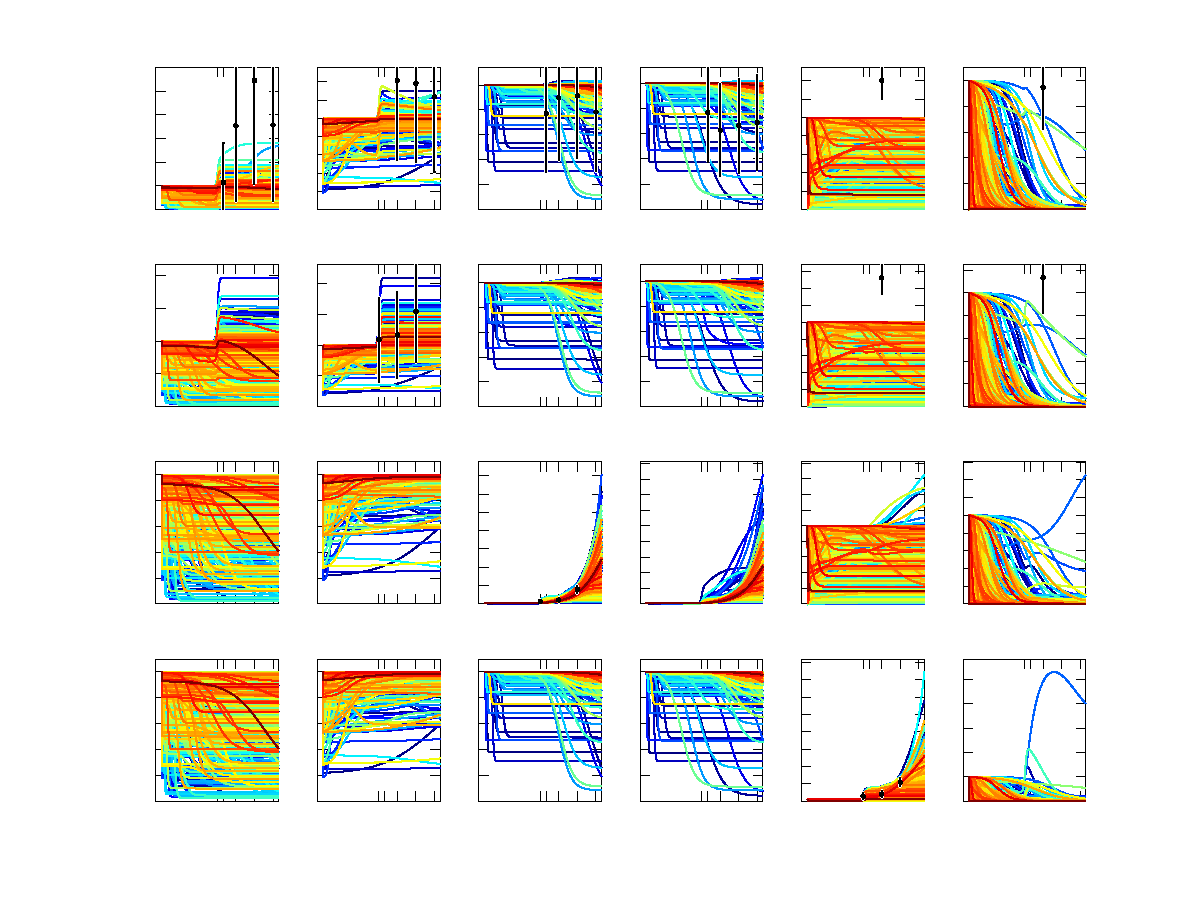
\includegraphics{SampleOutputsTauUpper}}%
    \gplfronttext
  \end{picture}%
\endgroup
};
    \node (Ytitle) at (plot.north) {model outputs};
    \foreach \i in {1,...,6} \node (Ylabel\i) at (-9.25+2.75*\i,7) {$y_\i$};
    \node (Tlabel) at (plot.south) {time $t$ in h};
    \node (Tdescription) [above of=Tlabel] {measurements were taken at $\{0.1,\,8,\,24,\,48,\,72\}$ h};
    \node (Utitle) at (-9,0) [rotate=90]{experiment conditions (inputs)};
    \foreach \i in {1,...,5} \node (Ulabel\i) at (-8.5,8.4-2.66*\i) {$u_\i$};
  \end{tikzpicture}
  \captionof{figure}{output trajectories per parameter sample member;
    to reduce the number of lines these trajectory lines are once
    again plotted for every 3534th
    ($2(\tau_{\text{int.},l}+\delta_\tau)$) parameter in the parameter
    sample. The green, vertical errorbars represent the data and its
    measurement error estimation. The data is sparse (not all outputs
    were observed at all measurement instances. The model does not fit
    all data points.)\label{fig:osmpl}}
\end{center}

\begin{center}
  \begin{tabular}{rl}
    \toprule
    tuning duration& $1000$ points\\
    target acceptance $a_0$&$0.50$\\
    observed acceptance $a$&$0.27$\\
    auto-correlation length $\tau_{\text{int.},l}$&$1516(250)$\\
    failed Likelihood evaluations \texttt{[CVODES]}&$16$\\
    \bottomrule
  \end{tabular}
  \captionof{table}{Sample Properties.\label{tab:sp}}
\end{center}


% The sample has the following correlation between the parameters:
% \begin{equation}
%   \label{eq:corrcoef}
%   C=
%   \begin{pmatrix}
%     1.00 & 0.89 & 0.85 & 0.81 & 0.85 & 0.79 & 0.79 & 0.86 & 0.80 & 0.78 & 0.79 & 0.82 & 0.88 & 0.84 & 0.89 & 0.89 & 0.82 & 0.87 & 0.78 & 0.88 & 0.82 & 0.84 & 0.85 & 0.84 & 0.87 & 0.81\\
0.84 & 0.80 & 0.80 & 0.82 & 0.84 & 0.79 & 0.83 & 0.82 & 0.82 & 0.87 & 0.86 & 0.83 & 0.81 & 0.83 & 0.86 & 0.81 & 0.80 & 0.83 & 0.78 & 0.80 & 0.81 & 0.82 & 0.88 & 0.84 & 0.81 & 0.77\\
0.74 & 0.93 & 0.82 & 0.76 & 0.79 & 0.77 & 0.88 & 0.84 & 0.80 & 0.88 & 0.83 & 0.84 & 0.85 & 0.85 & 0.84 & 0.79 & 0.81 & 0.75 & 0.82 & 0.86 & 0.85 & 0.84 & 0.84 & 0.83 & 0.89 & 0.85\\
0.85 & 0.85 & 0.86 & 0.86 & 0.84 & 0.78 & 0.82 & 0.83 & 0.87 & 0.86 & 0.87 & 0.80 & 0.83 & 0.86 & 0.81 & 0.86 & 0.87 & 0.81 & 0.81 & 0.81 & 0.84 & 0.88 & 0.86 & 0.88 & 0.83 & 0.71\\
0.82 & 0.84 & 0.81 & 0.83 & 0.79 & 0.75 & 0.86 & 0.88 & 0.86 & 0.84 & 0.81 & 0.82 & 0.81 & 0.85 & 0.80 & 0.85 & 0.86 & 0.78 & 0.86 & 0.87 & 0.78 & 0.86 & 0.89 & 0.84 & 0.81 & 0.85\\
0.88 & 0.82 & 0.84 & 0.79 & 0.75 & 0.82 & 0.87 & 0.79 & 0.83 & 0.81 & 0.83 & 0.87 & 0.81 & 0.83 & 0.75 & 0.87 & 0.84 & 0.78 & 0.86 & 0.81 & 0.87 & 0.89 & 0.80 & 0.83 & 0.83 & 0.85\\
0.81 & 0.88 & 0.76 & 0.85 & 0.86 & 0.86 & 0.93 & 0.87 & 0.81 & 0.85 & 0.77 & 0.83 & 0.88 & 0.78 & 0.84 & 0.90 & 0.78 & 0.81 & 0.82 & 0.85 & 0.82 & 0.78 & 0.87 & 0.83 & 0.85 & 0.85\\
0.81 & 0.84 & 0.83 & 0.75 & 0.80 & 0.83 & 0.77 & 0.83 & 0.80 & 0.84 & 0.81 & 0.85 & 0.87 & 0.81 & 0.90 & 0.84 & 0.82 & 0.78 & 0.85 & 0.74 & 0.77 & 0.83 & 0.90 & 0.88 & 0.84 & 0.84\\
0.86 & 0.85 & 0.85 & 0.83 & 0.84 & 0.89 & 0.87 & 0.80 & 0.87 & 0.84 & 0.86 & 0.83 & 0.85 & 0.82 & 0.84 & 0.79 & 0.80 & 0.85 & 0.81 & 0.83 & 0.88 & 0.86 & 0.86 & 0.87 & 0.83 & 0.83\\
0.80 & 0.85 & 0.82 & 0.83 & 0.77 & 0.87 & 0.88 & 0.88 & 0.79 & 0.80 & 0.86 & 0.76 & 0.77 & 0.78 & 0.87 & 0.85 & 0.85 & 0.86 & 0.84 & 0.88 & 0.85 & 0.86 & 0.85 & 0.80 & 0.83 & 0.84\\
0.82 & 0.83 & 0.76 & 0.82 & 0.76 & 0.89 & 0.83 & 0.86 & 0.86 & 0.82 & 0.88 & 0.78 & 0.85 & 0.85 & 0.88 & 0.83 & 0.76 & 0.83 & 0.86 & 0.86 & 0.85 & 0.85 & 0.89 & 1.00 & 0.86 & 0.84\\
0.82 & 0.77 & 0.76 & 0.84 & 0.83 & 0.77 & 0.84 & 0.78 & 0.85 & 0.88 & 0.85 & 0.90 & 0.84 & 0.85 & 0.79 & 0.86 & 0.79 & 0.83 & 0.81 & 0.86 & 0.84 & 0.90 & 0.88 & 0.84 & 0.86 & 0.85\\
0.86 & 0.80 & 0.86 & 0.80 & 0.82 & 0.87 & 0.83 & 0.81 & 0.83 & 0.85 & 0.86 & 0.83 & 0.82 & 0.83 & 0.82 & 0.80 & 0.82 & 0.84 & 0.86 & 0.79 & 0.83 & 0.83 & 0.72 & 0.91 & 0.80 & 0.78\\
0.82 & 0.78 & 0.89 & 0.81 & 0.75 & 0.88 & 0.86 & 0.83 & 0.86 & 0.88 & 0.86 & 0.84 & 0.83 & 0.81 & 0.86 & 0.90 & 0.88 & 0.82 & 0.88 & 0.85 & 0.89 & 0.83 & 0.87 & 0.87 & 0.86 & 0.85\\
0.85 & 0.77 & 0.88 & 0.87 & 0.86 & 0.84 & 0.85 & 0.84 & 0.84 & 0.84 & 0.77 & 0.88 & 0.87 & 0.74 & 0.86 & 0.77 & 0.88 & 0.90 & 0.90 & 0.89 & 0.84 & 0.73 & 0.82 & 0.86 & 0.77 & 0.86\\
0.80 & 0.77 & 0.84 & 0.89 & 0.86 & 0.83 & 0.74 & 0.85 & 0.81 & 0.85 & 0.79 & 0.87 & 0.84 & 0.78 & 0.84 & 0.83 & 0.75 & 0.83 & 0.82 & 0.84 & 0.84 & 0.85 & 0.87 & 0.80 & 0.86 & 0.77\\
0.73 & 0.86 & 0.84 & 0.83 & 0.76 & 0.78 & 0.81 & 0.84 & 0.71 & 0.80 & 0.82 & 0.81 & 0.82 & 0.74 & 0.79 & 0.89 & 0.81 & 0.85 & 0.75 & 0.74 & 0.86 & 0.78 & 0.91 & 0.87 & 0.75 & 0.86\\
0.85 & 0.80 & 0.89 & 0.86 & 0.86 & 0.91 & 0.75 & 0.87 & 0.89 & 0.80 & 0.82 & 0.90 & 0.82 & 0.88 & 0.92 & 0.90 & 0.83 & 0.77 & 0.87 & 0.87 & 0.88 & 0.80 & 0.82 & 0.82 & 0.84 & 0.80\\
0.81 & 0.84 & 0.79 & 0.84 & 0.81 & 0.87 & 0.81 & 0.86 & 0.86 & 0.81 & 0.90 & 0.87 & 0.80 & 0.81 & 0.84 & 0.74 & 0.79 & 0.84 & 0.86 & 0.95 & 0.82 & 0.80 & 0.88 & 0.89 & 0.86 & 0.89\\
0.84 & 0.87 & 0.87 & 0.73 & 0.88 & 0.88 & 0.82 & 0.80 & 0.82 & 0.82 & 0.86 & 0.79 & 0.79 & 0.82 & 0.79 & 0.85 & 0.85 & 0.88 & 0.88 & 0.89 & 0.83 & 0.85 & 0.78 & 0.85 & 0.85 & 0.86\\
0.76 & 0.81 & 0.87 & 0.78 & 0.85 & 0.80 & 0.90 & 0.77 & 0.78 & 0.76 & 0.87 & 0.86 & 0.77 & 0.82 & 0.86 & 0.84 & 0.86 & 0.87 & 0.88 & 0.85 & 0.80 & 0.83 & 0.81 & 0.86 & 0.79 & 0.81\\
0.79 & 0.88 & 0.75 & 0.86 & 0.83 & 0.81 & 0.88 & 0.80 & 0.87 & 0.86 & 0.84 & 0.83 & 0.70 & 0.86 & 0.89 & 0.86 & 0.81 & 0.85 & 0.85 & 0.86 & 1.00 & 0.79 & 0.81 & 0.76 & 0.79 & 0.82\\
0.81 & 0.79 & 0.81 & 0.82 & 0.83 & 0.82 & 0.84 & 0.83 & 0.78 & 0.81 & 0.73 & 0.84 & 0.81 & 0.84 & 0.79 & 0.82 & 0.80 & 0.81 & 0.81 & 0.75 & 0.83 & 0.74 & 0.83 & 0.79 & 0.83 & 0.79\\
0.87 & 0.79 & 0.78 & 0.79 & 0.81 & 0.81 & 0.78 & 0.80 & 0.80 & 0.82 & 0.78 & 0.82 & 0.83 & 0.82 & 0.84 & 0.83 & 0.84 & 0.79 & 0.77 & 0.90 & 0.73 & 0.77 & 0.74 & 0.83 & 0.87 & 0.79\\
0.77 & 0.81 & 0.81 & 0.82 & 0.87 & 0.80 & 0.84 & 0.82 & 0.80 & 0.80 & 0.82 & 0.82 & 0.80 & 0.82 & 0.80 & 0.80 & 0.83 & 0.83 & 0.79 & 0.82 & 0.81 & 0.81 & 0.79 & 0.75 & 0.84 & 0.81\\
0.84 & 0.83 & 0.81 & 0.82 & 0.86 & 0.85 & 0.82 & 0.79 & 0.82 & 0.74 & 0.76 & 0.81 & 0.82 & 0.85 & 0.78 & 0.85 & 0.78 & 0.68 & 0.84 & 0.80 & 0.81 & 0.83 & 0.86 & 0.85 & 0.82 & 0.81\\
0.83 & 0.74 & 0.82 & 0.77 & 0.83 & 0.80 & 0.80 & 0.84 & 0.83 & 0.76 & 0.82 & 0.80 & 0.82 & 0.76 & 0.84 & 0.79 & 0.77 & 0.82 & 0.82 & 0.72 & 0.83 & 0.76 & 0.79 & 0.83 & 0.78 & 0.79\\
0.80 & 0.82 & 0.81 & 0.81 & 0.81 & 0.82 & 0.80 & 0.85 & 0.81 & 0.80 & 0.84 & 0.78 & 0.86 & 0.80 & 0.81 & 0.81 & 0.84 & 0.83 & 0.76 & 0.83 & 0.83 & 0.86 & 0.85 & 0.84 & 0.81 & 0.84\\
0.78 & 0.79 & 0.79 & 0.84 & 0.80 & 0.79 & 0.75 & 0.82 & 0.84 & 0.83 & 0.80 & 0.80 & 0.81 & 0.75 & 0.86 & 0.83 & 0.74 & 0.79 & 0.80 & 0.83 & 0.80 & 0.76 & 0.81 & 0.86 & 0.86 & 0.83\\
0.80 & 0.81 & 0.77 & 0.85 & 0.81 & 0.81 & 0.88 & 0.86 & 0.78 & 0.76 & 0.78 & 0.73 & 0.78 & 0.79 & 0.84 & 0.90 & 0.78 & 0.83 & 0.81 & 0.76 & 0.80 & 0.81 & 0.87 & 0.84 & 0.83 & 0.78\\
0.83 & 0.81 & 0.81 & 0.83 & 0.77 & 0.80 & 0.83 & 0.81 & 0.79 & 0.84 & 0.78 & 0.78 & 0.82 & 0.83 & 0.80 & 0.80 & 0.85 & 0.84 & 0.83 & 0.79 & 0.78 & 0.78 & 0.72 & 0.79 & 0.79 & 0.81\\
0.82 & 0.81 & 0.78 & 0.77 & 0.79 & 0.79 & 0.83 & 0.88 & 0.78 & 0.82 & 0.80 & 0.84 & 0.79 & 0.82 & 0.83 & 0.80 & 0.84 & 0.84 & 0.82 & 0.85 & 0.82 & 0.85 & 0.82 & 0.85 & 0.84 & 0.86\\
0.83 & 0.82 & 0.83 & 0.80 & 0.87 & 0.82 & 0.82 & 0.82 & 0.68 & 0.83 & 0.82 & 0.78 & 0.80 & 0.83 & 0.81 & 0.84 & 0.79 & 1.00 & 0.82 & 0.84 & 0.81 & 0.88 & 0.83 & 0.80 & 0.89 & 0.75\\
0.86 & 0.88 & 0.85 & 0.86 & 0.86 & 0.83 & 0.85 & 0.87 & 0.85 & 0.87 & 0.82 & 0.89 & 0.86 & 0.86 & 0.88 & 0.87 & 0.86 & 0.86 & 0.86 & 0.83 & 0.89 & 0.83 & 0.86 & 0.88 & 0.83 & 0.83\\
0.88 & 0.84 & 0.86 & 0.86 & 0.80 & 0.84 & 0.79 & 0.82 & 0.79 & 0.87 & 0.92 & 0.80 & 0.91 & 0.89 & 0.78 & 0.82 & 0.73 & 0.81 & 0.80 & 0.81 & 0.67 & 0.86 & 0.81 & 0.87 & 0.83 & 0.88\\
0.89 & 0.88 & 0.88 & 0.84 & 0.84 & 0.87 & 0.86 & 0.91 & 0.82 & 0.82 & 0.89 & 0.82 & 0.91 & 0.84 & 0.89 & 0.88 & 0.85 & 0.91 & 0.89 & 0.84 & 0.93 & 0.90 & 0.87 & 0.87 & 0.89 & 0.85\\
0.86 & 0.83 & 0.79 & 0.87 & 0.84 & 0.79 & 0.87 & 0.81 & 0.78 & 0.84 & 0.86 & 0.93 & 0.87 & 0.84 & 0.82 & 0.89 & 0.84 & 0.88 & 0.83 & 0.81 & 0.86 & 0.92 & 0.92 & 0.87 & 0.80 & 0.83\\
0.82 & 0.91 & 0.77 & 0.93 & 0.88 & 0.84 & 0.87 & 0.89 & 0.83 & 0.84 & 0.92 & 0.90 & 0.76 & 0.89 & 0.88 & 0.83 & 0.90 & 0.82 & 0.78 & 0.91 & 0.88 & 0.77 & 0.78 & 0.79 & 0.85 & 0.88\\
0.76 & 0.84 & 0.81 & 0.85 & 0.84 & 0.79 & 0.83 & 0.88 & 0.89 & 0.81 & 0.79 & 0.76 & 0.89 & 0.84 & 0.87 & 0.89 & 0.80 & 0.87 & 0.86 & 0.87 & 0.83 & 0.90 & 0.87 & 0.90 & 0.73 & 0.86\\
0.87 & 0.82 & 0.76 & 0.89 & 0.83 & 0.91 & 0.91 & 0.91 & 0.82 & 0.77 & 0.91 & 0.89 & 0.87 & 0.82 & 0.77 & 0.86 & 0.89 & 0.86 & 0.88 & 0.85 & 0.79 & 0.85 & 0.79 & 0.91 & 0.76 & 0.90\\
0.88 & 0.85 & 0.81 & 0.80 & 0.85 & 0.83 & 0.91 & 0.79 & 0.82 & 0.84 & 0.88 & 0.82 & 0.84 & 0.83 & 0.88 & 0.85 & 0.82 & 0.89 & 0.86 & 0.91 & 0.92 & 0.85 & 0.86 & 0.91 & 0.81 & 0.80\\
0.80 & 0.82 & 0.83 & 0.80 & 0.80 & 0.88 & 0.82 & 0.85 & 0.84 & 0.86 & 0.88 & 0.87 & 0.88 & 0.92 & 0.85 & 0.84 & 0.85 & 0.81 & 0.84 & 0.82 & 0.86 & 0.85 & 0.92 & 0.85 & 0.86 & 0.78\\
0.73 & 0.81 & 0.85 & 0.92 & 0.81 & 0.86 & 0.88 & 0.89 & 0.86 & 0.87 & 0.92 & 0.85 & 0.78 & 0.80 & 0.83 & 0.87 & 0.86 & 0.89 & 0.80 & 0.86 & 0.68 & 0.88 & 0.91 & 0.91 & 0.84 & 0.88\\
0.89 & 0.88 & 0.85 & 0.87 & 0.75 & 0.91 & 0.89 & 0.84 & 0.79 & 0.88 & 0.85 & 0.82 & 0.81 & 0.82 & 1.00 & 0.89 & 0.90 & 0.92 & 0.88 & 0.86 & 0.85 & 0.89 & 0.91 & 0.91 & 0.91 & 0.93\\
0.92 & 0.94 & 0.90 & 0.93 & 0.92 & 0.87 & 0.95 & 0.92 & 0.91 & 0.90 & 0.92 & 0.90 & 0.89 & 0.90 & 0.93 & 0.91 & 0.94 & 0.92 & 0.89 & 0.92 & 0.90 & 0.93 & 0.88 & 0.90 & 0.94 & 0.92\\
0.84 & 0.91 & 0.92 & 0.91 & 0.90 & 0.97 & 0.93 & 0.90 & 0.93 & 0.91 & 0.88 & 0.87 & 0.80 & 0.94 & 0.93 & 0.82 & 0.79 & 0.87 & 0.92 & 0.91 & 0.94 & 0.93 & 0.90 & 0.94 & 0.93 & 0.85\\
0.95 & 0.92 & 0.89 & 0.92 & 0.90 & 0.89 & 0.94 & 0.85 & 0.93 & 0.91 & 0.89 & 0.93 & 0.93 & 0.90 & 0.88 & 0.87 & 0.90 & 0.89 & 0.93 & 0.94 & 0.93 & 0.90 & 0.91 & 0.89 & 0.92 & 0.90\\
0.90 & 0.92 & 0.92 & 0.95 & 0.88 & 0.92 & 0.89 & 0.89 & 0.89 & 0.83 & 0.95 & 0.92 & 0.89 & 0.91 & 0.90 & 0.90 & 0.89 & 0.91 & 0.95 & 0.84 & 0.87 & 0.94 & 0.88 & 0.88 & 0.88 & 0.90\\
0.92 & 0.86 & 0.87 & 0.91 & 0.89 & 0.86 & 0.89 & 0.88 & 0.88 & 0.87 & 0.92 & 0.88 & 0.89 & 0.93 & 0.90 & 0.88 & 0.90 & 0.90 & 0.87 & 0.89 & 0.94 & 0.94 & 0.92 & 0.95 & 0.88 & 0.92\\
0.94 & 0.91 & 0.92 & 0.82 & 0.89 & 0.94 & 0.89 & 0.86 & 0.93 & 0.93 & 0.90 & 0.95 & 0.86 & 0.93 & 0.93 & 0.87 & 0.85 & 0.89 & 0.93 & 0.91 & 0.83 & 0.94 & 0.91 & 0.93 & 0.89 & 0.94\\
0.91 & 0.91 & 0.90 & 0.87 & 0.88 & 0.91 & 0.93 & 0.93 & 0.89 & 0.87 & 0.91 & 0.94 & 0.91 & 0.93 & 0.95 & 0.90 & 0.89 & 0.94 & 0.91 & 0.90 & 0.81 & 0.92 & 0.88 & 0.96 & 0.90 & 0.89\\
0.88 & 0.90 & 0.87 & 0.89 & 0.92 & 0.96 & 0.96 & 0.82 & 0.92 & 0.92 & 0.92 & 0.88 & 0.92 & 0.93 & 0.91 & 0.92 & 0.93 & 0.88 & 0.87 & 0.91 & 0.91 & 0.89 & 0.91 & 0.80 & 0.92 & 0.88\\
0.89 & 0.90 & 0.92 & 0.89 & 0.96 & 0.89 & 0.92 & 0.90 & 0.94 & 0.89 & 0.87 & 0.93 & 0.90 & 0.91 & 0.90 & 0.91 & 0.93 & 0.89 & 0.89 & 0.95 & 0.87 & 0.81 & 0.87 & 0.90 & 0.91 & 0.93\\
0.90 & 0.93 & 0.90 & 0.91 & 0.94 & 0.95 & 0.92 & 0.88 & 0.92 & 0.94 & 0.90 & 0.92 & 0.92 & 0.94 & 0.93 & 0.91 & 0.80 & 0.90 & 0.92 & 0.88 & 0.94 & 0.89 & 0.88 & 0.94 & 0.97 & 0.90\\
0.84 & 0.91 & 0.91 & 0.91 & 0.91 & 0.90 & 0.79 & 0.77 & 0.76 & 0.84 & 0.89 & 1.00 & 0.91 & 0.87 & 0.92 & 0.86 & 0.85 & 0.86 & 0.82 & 0.87 & 0.88 & 0.86 & 0.88 & 0.89 & 0.88 & 0.89\\
0.92 & 0.85 & 0.94 & 0.87 & 0.85 & 0.85 & 0.88 & 0.91 & 0.85 & 0.86 & 0.88 & 0.94 & 0.89 & 0.93 & 0.82 & 0.87 & 0.88 & 0.90 & 0.95 & 0.85 & 0.89 & 0.92 & 0.92 & 0.87 & 0.80 & 0.83\\
0.87 & 0.88 & 0.90 & 0.88 & 0.88 & 0.92 & 0.83 & 0.79 & 0.82 & 0.94 & 0.91 & 0.86 & 0.71 & 0.88 & 0.94 & 0.91 & 0.83 & 0.93 & 0.88 & 0.88 & 0.87 & 0.83 & 0.91 & 0.90 & 0.86 & 0.87\\
0.87 & 0.88 & 0.91 & 0.86 & 0.92 & 0.86 & 0.88 & 0.87 & 0.86 & 0.89 & 0.87 & 0.94 & 0.85 & 0.93 & 0.85 & 0.86 & 0.87 & 0.86 & 0.90 & 0.85 & 0.92 & 0.87 & 0.84 & 0.90 & 0.90 & 0.94\\
0.86 & 0.86 & 0.85 & 0.84 & 0.94 & 0.94 & 0.87 & 0.92 & 0.84 & 0.88 & 0.90 & 0.87 & 0.82 & 0.87 & 0.89 & 0.90 & 0.87 & 0.87 & 0.87 & 0.85 & 0.86 & 0.87 & 0.90 & 0.93 & 0.87 & 0.87\\
0.87 & 0.88 & 0.83 & 0.86 & 0.83 & 0.95 & 0.87 & 0.81 & 0.86 & 0.94 & 0.89 & 0.80 & 0.89 & 0.83 & 0.88 & 0.86 & 0.83 & 0.90 & 0.86 & 0.94 & 0.88 & 0.90 & 0.88 & 0.90 & 0.88 & 0.80\\
0.87 & 0.88 & 0.86 & 0.89 & 0.88 & 0.93 & 0.87 & 0.86 & 0.83 & 0.92 & 0.86 & 0.87 & 0.80 & 0.85 & 0.87 & 0.87 & 0.84 & 0.93 & 0.88 & 0.86 & 0.89 & 0.85 & 0.90 & 0.83 & 0.89 & 0.89\\
0.88 & 0.86 & 0.87 & 0.91 & 0.86 & 0.86 & 0.86 & 0.85 & 0.86 & 0.90 & 0.92 & 0.81 & 0.80 & 0.94 & 0.86 & 0.87 & 0.77 & 0.92 & 0.83 & 0.90 & 0.83 & 0.83 & 0.92 & 0.86 & 0.83 & 0.92\\
0.94 & 0.88 & 0.88 & 0.77 & 0.87 & 0.81 & 0.91 & 0.85 & 0.86 & 0.86 & 0.88 & 0.87 & 0.89 & 0.85 & 0.84 & 0.86 & 0.94 & 0.95 & 0.88 & 0.85 & 0.89 & 0.84 & 0.88 & 0.92 & 0.97 & 0.85\\
0.84 & 0.90 & 0.89 & 0.92 & 0.89 & 0.89 & 0.87 & 0.86 & 0.88 & 0.83 & 0.94 & 0.87 & 0.81 & 0.88 & 0.89 & 0.91 & 0.86 & 0.88 & 0.81 & 0.83 & 0.86 & 0.90 & 0.80 & 0.86 & 0.87 & 0.93\\
0.88 & 0.88 & 0.88 & 0.89 & 0.87 & 0.91 & 0.95 & 0.84 & 0.94 & 0.86 & 0.89 & 0.85 & 0.77 & 0.87 & 0.89 & 0.90 & 0.89 & 0.95 & 0.90 & 0.85 & 0.90 & 0.84 & 0.79 & 0.86 & 0.86 & 0.85\\
0.86 & 0.93 & 0.79 & 0.76 & 0.79 & 0.81 & 0.90 & 0.91 & 1.00 & 0.92 & 0.91 & 0.88 & 0.92 & 0.92 & 0.88 & 0.89 & 0.91 & 0.90 & 0.88 & 0.86 & 0.87 & 0.91 & 0.93 & 0.88 & 0.93 & 0.93\\
0.86 & 0.84 & 0.88 & 0.83 & 0.88 & 0.88 & 0.91 & 0.96 & 0.92 & 0.93 & 0.88 & 0.87 & 0.89 & 0.91 & 0.96 & 0.86 & 0.89 & 0.94 & 0.95 & 0.89 & 0.79 & 0.94 & 0.88 & 0.88 & 0.90 & 0.93\\
0.92 & 0.89 & 0.87 & 0.77 & 0.73 & 0.89 & 0.83 & 0.88 & 0.74 & 0.85 & 0.93 & 0.94 & 0.86 & 0.91 & 0.91 & 0.90 & 0.91 & 0.90 & 0.94 & 0.90 & 0.89 & 0.86 & 0.89 & 0.90 & 0.87 & 0.85\\
0.91 & 0.89 & 0.90 & 0.88 & 0.90 & 0.92 & 0.91 & 0.95 & 0.89 & 0.91 & 0.90 & 0.90 & 0.93 & 0.91 & 0.92 & 0.90 & 0.93 & 0.92 & 0.89 & 0.94 & 0.91 & 0.95 & 0.89 & 0.90 & 0.86 & 0.84\\
0.95 & 0.82 & 0.93 & 0.94 & 0.89 & 0.93 & 0.91 & 0.85 & 0.84 & 0.87 & 0.87 & 0.89 & 0.87 & 0.87 & 0.91 & 0.88 & 0.89 & 0.88 & 0.94 & 0.92 & 0.88 & 0.84 & 0.94 & 0.87 & 0.88 & 0.89\\
0.91 & 0.89 & 0.94 & 0.92 & 0.86 & 0.93 & 0.92 & 0.87 & 0.86 & 0.86 & 0.91 & 0.93 & 0.87 & 0.94 & 0.92 & 0.96 & 0.90 & 0.95 & 0.90 & 0.94 & 0.88 & 0.83 & 0.87 & 0.89 & 0.91 & 0.89\\
0.89 & 0.96 & 0.87 & 0.92 & 0.88 & 0.95 & 0.92 & 0.89 & 0.86 & 0.90 & 0.86 & 0.86 & 0.86 & 0.95 & 0.90 & 0.93 & 0.88 & 0.89 & 0.93 & 0.86 & 0.89 & 0.87 & 0.92 & 0.95 & 0.90 & 0.92\\
0.87 & 0.89 & 0.89 & 0.90 & 0.91 & 0.87 & 0.90 & 0.86 & 0.88 & 0.94 & 0.87 & 0.86 & 0.82 & 0.94 & 0.89 & 0.89 & 0.88 & 0.84 & 0.97 & 0.82 & 0.84 & 0.95 & 0.93 & 0.91 & 0.90 & 0.81\\
0.84 & 0.86 & 0.91 & 0.86 & 0.92 & 0.90 & 0.93 & 0.89 & 0.93 & 0.89 & 0.90 & 0.88 & 0.93 & 0.94 & 0.91 & 0.89 & 0.95 & 0.86 & 0.91 & 0.95 & 0.95 & 0.89 & 0.85 & 0.89 & 0.93 & 0.88\\
0.92 & 0.92 & 0.90 & 0.88 & 0.88 & 0.87 & 0.88 & 0.90 & 0.89 & 0.89 & 0.90 & 0.95 & 0.85 & 0.84 & 0.86 & 0.85 & 0.90 & 0.91 & 0.85 & 0.90 & 0.92 & 0.93 & 0.88 & 0.89 & 0.91 & 0.92\\
0.89 & 0.96 & 0.95 & 0.84 & 0.95 & 0.88 & 0.95 & 0.91 & 0.82 & 0.90 & 0.90 & 0.88 & 0.91 & 0.94 & 0.90 & 0.89 & 0.88 & 0.89 & 0.78 & 0.93 & 0.87 & 0.90 & 0.95 & 0.93 & 0.86 & 0.84\\
0.82 & 0.88 & 0.92 & 0.87 & 0.92 & 1.00 & 0.88 & 0.88 & 0.92 & 0.87 & 0.93 & 0.94 & 0.93 & 0.94 & 0.93 & 0.95 & 0.89 & 0.96 & 0.94 & 0.90 & 0.93 & 0.92 & 0.91 & 0.91 & 0.91 & 0.88\\
0.95 & 0.92 & 0.93 & 0.92 & 0.95 & 0.91 & 0.93 & 0.93 & 0.92 & 0.91 & 0.92 & 0.93 & 0.91 & 0.93 & 0.89 & 0.89 & 0.88 & 0.90 & 0.89 & 0.90 & 0.96 & 0.90 & 0.93 & 0.90 & 0.84 & 0.89\\
0.78 & 0.88 & 0.84 & 0.84 & 0.77 & 0.90 & 0.93 & 0.92 & 0.93 & 0.91 & 0.96 & 0.94 & 0.91 & 0.93 & 0.90 & 0.88 & 0.92 & 0.93 & 0.93 & 0.88 & 0.93 & 0.90 & 0.94 & 0.91 & 0.90 & 0.95\\
0.94 & 0.93 & 0.94 & 0.87 & 0.95 & 0.92 & 0.94 & 0.96 & 0.96 & 0.91 & 0.92 & 0.91 & 0.88 & 0.94 & 0.93 & 0.89 & 0.93 & 0.93 & 0.87 & 0.95 & 0.92 & 0.92 & 0.93 & 0.79 & 0.93 & 0.95\\
0.91 & 0.93 & 0.90 & 0.86 & 0.95 & 0.95 & 0.93 & 0.89 & 0.86 & 0.92 & 0.89 & 0.95 & 0.90 & 0.94 & 0.93 & 0.87 & 0.94 & 0.93 & 0.92 & 0.86 & 0.93 & 0.92 & 0.91 & 0.90 & 0.94 & 0.92\\
0.90 & 0.89 & 0.91 & 0.90 & 0.91 & 0.91 & 0.87 & 0.91 & 0.94 & 0.94 & 0.86 & 0.94 & 0.90 & 0.96 & 0.93 & 0.90 & 0.93 & 0.92 & 0.92 & 0.92 & 0.91 & 0.84 & 0.96 & 0.93 & 0.88 & 0.96\\
0.88 & 0.94 & 0.93 & 0.93 & 0.90 & 0.90 & 0.93 & 0.94 & 0.90 & 0.94 & 0.96 & 0.92 & 0.92 & 0.96 & 0.91 & 0.92 & 0.92 & 0.93 & 0.90 & 0.90 & 0.93 & 0.94 & 0.90 & 0.88 & 0.92 & 0.90\\
0.91 & 0.89 & 0.93 & 0.92 & 0.88 & 0.95 & 0.89 & 0.95 & 0.87 & 0.92 & 0.92 & 0.92 & 0.92 & 0.85 & 0.94 & 0.88 & 0.94 & 0.91 & 0.89 & 0.92 & 0.94 & 0.85 & 0.93 & 0.91 & 0.94 & 0.94\\
0.92 & 0.94 & 0.96 & 0.96 & 0.97 & 0.89 & 0.94 & 0.95 & 0.94 & 0.91 & 0.91 & 0.87 & 0.91 & 0.86 & 0.91 & 0.95 & 0.90 & 0.94 & 0.93 & 0.93 & 0.94 & 0.92 & 0.94 & 0.93 & 0.88 & 0.93\\
0.92 & 0.94 & 0.87 & 0.94 & 0.96 & 0.89 & 0.92 & 0.93 & 0.89 & 0.84 & 0.84 & 0.84 & 0.98 & 0.93 & 0.87 & 0.93 & 0.96 & 0.93 & 0.94 & 0.94 & 0.93 & 0.93 & 0.93 & 0.92 & 0.90 & 0.89\\
0.89 & 0.91 & 0.90 & 0.94 & 0.77 & 0.93 & 0.94 & 0.90 & 0.93 & 0.92 & 0.94 & 0.92 & 0.94 & 0.92 & 0.83 & 0.97 & 0.92 & 0.96 & 0.91 & 0.95 & 0.80 & 0.83 & 0.81 & 0.83 & 0.88 & 0.92\\
0.91 & 0.88 & 1.00 & 0.89 & 0.87 & 0.91 & 0.82 & 0.92 & 0.89 & 0.91 & 0.89 & 0.91 & 0.83 & 0.95 & 0.89 & 0.91 & 0.89 & 0.88 & 0.83 & 0.92 & 0.91 & 0.90 & 0.88 & 0.85 & 0.94 & 0.91\\
0.93 & 0.90 & 0.87 & 0.83 & 0.88 & 0.87 & 0.93 & 0.88 & 0.90 & 0.92 & 0.89 & 0.92 & 0.82 & 0.88 & 0.91 & 0.93 & 0.89 & 0.87 & 0.91 & 0.91 & 0.85 & 0.85 & 0.80 & 0.92 & 0.89 & 0.87\\
0.76 & 0.84 & 0.90 & 0.92 & 0.92 & 0.90 & 0.93 & 0.89 & 0.90 & 0.90 & 0.92 & 0.91 & 0.93 & 0.86 & 0.92 & 0.90 & 0.92 & 0.90 & 0.95 & 0.85 & 0.92 & 0.89 & 0.93 & 0.89 & 0.91 & 0.89\\
0.91 & 0.92 & 0.91 & 0.88 & 0.91 & 0.96 & 0.94 & 0.88 & 0.89 & 0.92 & 0.91 & 0.84 & 0.92 & 0.91 & 0.89 & 0.89 & 0.93 & 0.86 & 0.95 & 0.88 & 0.94 & 0.92 & 0.80 & 0.95 & 0.93 & 0.90\\
0.82 & 0.91 & 0.87 & 0.89 & 0.88 & 0.87 & 0.89 & 0.86 & 0.92 & 0.90 & 0.90 & 0.91 & 0.88 & 0.85 & 0.91 & 0.90 & 0.85 & 0.87 & 0.90 & 0.93 & 0.89 & 0.80 & 0.91 & 0.90 & 0.89 & 0.88\\
0.88 & 0.90 & 0.91 & 0.90 & 0.84 & 0.91 & 0.87 & 0.93 & 0.92 & 0.90 & 0.89 & 0.87 & 0.88 & 0.88 & 0.86 & 0.88 & 0.88 & 0.87 & 0.92 & 0.91 & 0.91 & 0.90 & 0.90 & 0.93 & 0.89 & 0.81\\
0.85 & 0.86 & 0.89 & 0.87 & 0.88 & 0.96 & 0.91 & 0.88 & 0.88 & 0.87 & 0.94 & 0.90 & 0.91 & 0.92 & 0.92 & 0.90 & 0.90 & 0.92 & 0.85 & 0.87 & 0.91 & 0.85 & 0.84 & 0.88 & 0.90 & 0.85\\
0.88 & 0.91 & 0.91 & 0.91 & 0.87 & 0.93 & 0.84 & 0.89 & 0.90 & 0.85 & 0.91 & 0.88 & 0.88 & 0.89 & 0.91 & 0.88 & 0.88 & 0.87 & 0.89 & 0.88 & 0.94 & 0.89 & 0.90 & 0.91 & 0.94 & 0.90\\
0.91 & 0.87 & 0.89 & 0.91 & 0.92 & 0.91 & 0.90 & 0.89 & 0.91 & 0.93 & 0.93 & 0.93 & 0.94 & 0.85 & 0.87 & 0.91 & 0.89 & 0.94 & 0.91 & 0.90 & 0.89 & 0.90 & 0.93 & 0.89 & 0.85 & 0.83\\
0.83 & 0.86 & 0.93 & 0.90 & 0.88 & 0.94 & 0.85 & 0.85 & 0.91 & 0.91 & 0.81 & 0.91 & 0.88 & 0.92 & 0.89 & 0.90 & 0.92 & 0.91 & 0.91 & 0.93 & 0.92 & 0.90 & 0.93 & 0.86 & 0.92 & 0.91\\
0.77 & 0.88 & 0.87 & 0.88 & 0.89 & 0.94 & 0.92 & 0.86 & 0.91 & 0.87 & 0.70 & 0.89 & 0.93 & 0.87 & 0.90 & 0.94 & 0.78 & 0.77 & 0.79 & 0.80 & 0.86 & 0.86 & 0.88 & 0.88 & 0.89 & 1.00\\
0.91 & 0.94 & 0.90 & 0.91 & 0.86 & 0.90 & 0.85 & 0.87 & 0.83 & 0.89 & 0.85 & 0.83 & 0.87 & 0.86 & 0.83 & 0.90 & 0.84 & 0.79 & 0.92 & 0.84 & 0.94 & 0.87 & 0.89 & 0.86 & 0.88 & 0.80\\
0.94 & 0.83 & 0.86 & 0.83 & 0.84 & 0.94 & 0.89 & 0.90 & 0.82 & 0.90 & 0.89 & 0.86 & 0.89 & 0.94 & 0.90 & 0.87 & 0.91 & 0.82 & 0.71 & 0.84 & 0.88 & 0.79 & 0.68 & 0.90 & 0.91 & 0.89\\
0.87 & 0.90 & 0.92 & 0.85 & 0.90 & 0.88 & 0.87 & 0.79 & 0.86 & 0.87 & 0.86 & 0.91 & 0.83 & 0.95 & 0.89 & 0.90 & 0.93 & 0.88 & 0.90 & 0.89 & 0.92 & 0.85 & 0.90 & 0.89 & 0.90 & 0.88\\
0.83 & 0.92 & 0.92 & 0.92 & 0.86 & 0.82 & 0.90 & 0.86 & 0.84 & 0.86 & 0.82 & 0.87 & 0.84 & 0.88 & 0.89 & 0.75 & 0.89 & 0.88 & 0.85 & 0.86 & 0.96 & 0.91 & 0.88 & 0.87 & 0.86 & 0.87\\
0.93 & 0.83 & 0.89 & 0.90 & 0.94 & 0.84 & 0.86 & 0.77 & 0.88 & 0.86 & 0.95 & 0.88 & 0.85 & 0.86 & 0.89 & 0.89 & 0.86 & 0.78 & 0.91 & 0.84 & 0.87 & 0.85 & 0.81 & 0.85 & 0.94 & 0.92\\
0.87 & 0.89 & 0.91 & 0.89 & 0.90 & 0.91 & 0.90 & 0.88 & 0.88 & 0.84 & 0.89 & 0.85 & 0.95 & 0.89 & 0.86 & 0.91 & 0.82 & 0.84 & 0.91 & 0.92 & 0.86 & 0.87 & 0.86 & 0.90 & 0.84 & 0.85\\
0.88 & 0.92 & 0.90 & 0.90 & 0.85 & 0.88 & 0.91 & 0.82 & 0.86 & 0.85 & 0.93 & 0.86 & 0.85 & 0.90 & 0.84 & 0.91 & 0.92 & 0.85 & 0.80 & 0.88 & 0.87 & 0.88 & 0.85 & 0.93 & 0.94 & 0.85\\
0.90 & 0.91 & 0.86 & 0.82 & 0.84 & 0.80 & 0.88 & 0.87 & 0.82 & 0.86 & 0.83 & 0.87 & 0.86 & 0.78 & 0.86 & 0.91 & 0.84 & 0.86 & 0.87 & 0.88 & 0.93 & 0.86 & 0.90 & 0.91 & 0.94 & 0.87\\
0.91 & 0.88 & 0.94 & 0.92 & 0.90 & 0.94 & 0.89 & 0.90 & 0.88 & 0.86 & 0.88 & 0.88 & 0.85 & 0.90 & 0.91 & 0.88 & 0.89 & 0.93 & 0.92 & 0.88 & 0.81 & 0.83 & 0.85 & 0.88 & 0.91 & 0.91\\
0.90 & 0.93 & 0.87 & 0.91 & 0.87 & 0.87 & 0.78 & 0.86 & 0.90 & 0.91 & 0.83 & 0.84 & 0.88 & 0.91 & 0.91 & 0.92 & 0.93 & 0.90 & 0.88 & 0.85 & 0.87 & 0.90 & 0.83 & 0.86 & 0.87 & 0.92\\
0.88 & 0.90 & 0.91 & 0.87 & 0.89 & 0.88 & 0.71 & 0.87 & 0.85 & 0.90 & 0.91 & 0.92 & 0.79 & 0.84 & 0.81 & 0.89 & 0.85 & 0.85 & 0.92 & 0.92 & 0.87 & 0.91 & 1.00 & 0.86 & 0.92 & 0.93\\
0.86 & 0.89 & 0.87 & 0.85 & 0.86 & 0.91 & 0.88 & 0.83 & 0.85 & 0.92 & 0.82 & 0.87 & 0.85 & 0.80 & 0.95 & 0.86 & 0.91 & 0.90 & 0.92 & 0.87 & 0.89 & 0.85 & 0.92 & 0.83 & 0.93 & 0.84\\
0.84 & 0.93 & 0.91 & 0.84 & 0.79 & 0.90 & 0.83 & 0.86 & 0.90 & 0.89 & 0.91 & 0.87 & 0.81 & 0.82 & 0.70 & 0.81 & 0.82 & 0.87 & 0.73 & 0.88 & 0.85 & 0.91 & 0.86 & 0.90 & 0.92 & 0.89\\
0.90 & 0.91 & 0.90 & 0.88 & 0.88 & 0.89 & 0.87 & 0.87 & 0.85 & 0.89 & 0.90 & 0.87 & 0.94 & 0.92 & 0.90 & 0.92 & 0.96 & 0.88 & 0.94 & 0.93 & 0.91 & 0.90 & 0.88 & 0.90 & 0.88 & 0.89\\
0.88 & 0.89 & 0.87 & 0.83 & 0.90 & 0.85 & 0.88 & 0.92 & 0.85 & 0.89 & 0.92 & 0.76 & 0.90 & 0.92 & 0.91 & 0.89 & 0.91 & 0.83 & 0.86 & 0.91 & 0.88 & 0.92 & 0.82 & 0.88 & 0.86 & 0.93\\
0.84 & 0.91 & 0.93 & 0.84 & 0.92 & 0.85 & 0.90 & 0.87 & 0.89 & 0.93 & 0.87 & 0.89 & 0.90 & 0.85 & 0.90 & 0.85 & 0.86 & 0.87 & 0.84 & 0.81 & 0.89 & 0.87 & 0.85 & 0.92 & 0.82 & 0.88\\
0.90 & 0.90 & 0.85 & 0.84 & 0.85 & 0.87 & 0.90 & 0.85 & 0.88 & 0.80 & 0.89 & 0.88 & 0.88 & 0.87 & 0.83 & 0.92 & 0.92 & 0.87 & 0.86 & 0.92 & 0.87 & 0.90 & 0.79 & 0.92 & 0.90 & 0.87\\
0.86 & 0.92 & 0.93 & 0.87 & 0.92 & 0.91 & 0.89 & 0.87 & 0.87 & 0.92 & 0.87 & 0.87 & 0.87 & 0.87 & 0.88 & 0.88 & 0.91 & 0.86 & 0.84 & 0.93 & 0.86 & 0.87 & 0.81 & 0.91 & 0.89 & 0.85\\
0.87 & 0.87 & 0.93 & 0.86 & 0.85 & 0.87 & 0.90 & 0.87 & 0.85 & 0.83 & 0.87 & 0.84 & 0.87 & 0.86 & 0.86 & 0.91 & 0.94 & 0.89 & 0.94 & 0.84 & 0.93 & 0.90 & 0.89 & 0.90 & 0.88 & 0.87\\
0.91 & 0.84 & 0.84 & 0.91 & 0.86 & 0.94 & 0.85 & 0.88 & 0.90 & 0.88 & 0.89 & 0.92 & 0.85 & 0.93 & 0.85 & 0.89 & 0.84 & 0.86 & 0.90 & 0.86 & 0.95 & 0.91 & 0.88 & 0.85 & 0.82 & 0.81\\
0.90 & 0.90 & 0.79 & 0.86 & 0.95 & 0.90 & 0.85 & 0.89 & 0.90 & 0.94 & 0.88 & 0.91 & 0.93 & 0.87 & 0.91 & 0.86 & 0.91 & 0.91 & 0.77 & 0.91 & 0.88 & 0.92 & 0.89 & 0.90 & 0.95 & 0.88\\
0.84 & 0.92 & 0.74 & 0.92 & 0.87 & 0.92 & 0.88 & 0.90 & 0.82 & 0.78 & 0.82 & 0.75 & 0.89 & 0.86 & 0.92 & 0.87 & 0.91 & 0.94 & 0.86 & 1.00 & 0.88 & 0.86 & 0.88 & 0.92 & 0.84 & 0.88\\
0.78 & 0.91 & 0.85 & 0.87 & 0.88 & 0.85 & 0.81 & 0.88 & 0.87 & 0.80 & 0.88 & 0.83 & 0.93 & 0.88 & 0.91 & 0.85 & 0.87 & 0.81 & 0.90 & 0.85 & 0.86 & 0.83 & 0.86 & 0.92 & 0.89 & 0.93\\
0.78 & 0.91 & 0.92 & 0.89 & 0.87 & 0.94 & 0.88 & 0.83 & 0.91 & 0.82 & 0.70 & 0.84 & 0.86 & 0.77 & 0.74 & 0.82 & 0.90 & 0.90 & 0.90 & 0.89 & 0.93 & 0.87 & 0.90 & 0.89 & 0.87 & 0.81\\
0.87 & 0.83 & 0.88 & 0.93 & 0.84 & 0.92 & 0.92 & 0.88 & 0.91 & 0.85 & 0.91 & 0.89 & 0.88 & 0.85 & 0.87 & 0.86 & 0.92 & 0.87 & 0.87 & 0.92 & 0.92 & 0.93 & 0.90 & 0.85 & 0.89 & 0.87\\
0.84 & 0.89 & 0.85 & 0.89 & 0.88 & 0.87 & 0.89 & 0.73 & 0.91 & 0.87 & 0.83 & 0.91 & 0.94 & 0.90 & 0.86 & 0.87 & 0.83 & 0.84 & 0.93 & 0.83 & 0.89 & 0.87 & 0.95 & 0.83 & 0.88 & 0.79\\
0.89 & 0.85 & 0.95 & 0.88 & 0.85 & 0.83 & 0.89 & 0.85 & 0.89 & 0.80 & 0.89 & 0.85 & 0.88 & 0.87 & 0.84 & 0.90 & 0.96 & 0.94 & 0.88 & 0.91 & 0.95 & 0.91 & 0.88 & 0.91 & 0.90 & 0.89\\
0.87 & 0.80 & 0.88 & 0.86 & 0.92 & 0.95 & 0.87 & 0.93 & 0.84 & 0.89 & 0.92 & 0.92 & 0.87 & 0.86 & 0.88 & 0.89 & 0.81 & 0.81 & 0.89 & 0.93 & 0.90 & 0.92 & 0.84 & 0.87 & 0.90 & 0.82\\
0.86 & 0.86 & 0.94 & 0.89 & 0.86 & 0.88 & 0.80 & 0.89 & 0.94 & 0.86 & 0.80 & 0.84 & 0.86 & 0.89 & 0.89 & 0.90 & 0.95 & 0.84 & 0.92 & 0.92 & 0.86 & 0.84 & 0.88 & 0.80 & 0.88 & 0.84\\
0.81 & 0.87 & 0.83 & 0.87 & 0.89 & 0.80 & 0.86 & 0.90 & 0.86 & 0.87 & 0.89 & 0.86 & 0.93 & 0.87 & 0.89 & 0.91 & 0.92 & 0.85 & 0.91 & 0.89 & 0.90 & 0.92 & 0.93 & 0.94 & 0.90 & 0.92\\
0.89 & 0.84 & 0.87 & 0.86 & 0.86 & 0.89 & 0.91 & 0.86 & 0.89 & 0.91 & 0.92 & 0.84 & 0.76 & 0.82 & 0.86 & 0.86 & 0.86 & 0.89 & 0.86 & 0.93 & 0.92 & 0.90 & 0.89 & 0.88 & 0.82 & 0.87\\
0.90 & 0.91 & 0.84 & 0.86 & 0.87 & 0.90 & 0.92 & 0.96 & 0.93 & 0.90 & 0.88 & 0.84 & 0.89 & 0.91 & 0.82 & 0.85 & 0.85 & 0.88 & 0.90 & 0.88 & 0.89 & 0.87 & 0.91 & 0.86 & 0.68 & 0.86\\
0.87 & 0.87 & 0.93 & 0.90 & 0.88 & 0.85 & 0.83 & 0.86 & 0.91 & 0.82 & 0.88 & 0.93 & 0.82 & 0.90 & 0.92 & 0.88 & 1.00 & 0.94 & 0.92 & 0.95 & 0.84 & 0.88 & 0.87 & 0.92 & 0.86 & 0.87\\
0.87 & 0.92 & 0.90 & 0.88 & 0.90 & 0.79 & 0.91 & 0.91 & 0.91 & 0.86 & 0.93 & 0.87 & 0.91 & 0.90 & 0.96 & 0.89 & 0.86 & 0.89 & 0.92 & 0.92 & 0.86 & 0.87 & 0.81 & 0.89 & 0.86 & 0.90\\
0.94 & 0.93 & 0.91 & 0.86 & 0.82 & 0.86 & 0.69 & 0.79 & 0.83 & 0.77 & 0.76 & 0.92 & 0.85 & 0.91 & 0.88 & 0.93 & 0.91 & 0.91 & 0.94 & 0.85 & 0.88 & 0.82 & 0.87 & 0.93 & 0.88 & 0.93\\
0.86 & 0.89 & 0.92 & 0.93 & 0.93 & 0.93 & 0.93 & 0.95 & 0.93 & 0.82 & 0.94 & 0.90 & 0.95 & 0.93 & 0.90 & 0.88 & 0.89 & 0.93 & 0.85 & 0.88 & 0.92 & 0.87 & 0.86 & 0.84 & 0.83 & 0.92\\
0.88 & 0.94 & 0.89 & 0.72 & 0.90 & 0.90 & 0.89 & 0.88 & 0.90 & 0.84 & 0.94 & 0.94 & 0.92 & 0.90 & 0.87 & 0.92 & 0.87 & 0.96 & 0.85 & 0.91 & 0.94 & 0.77 & 0.91 & 0.88 & 0.89 & 0.92\\
0.91 & 0.96 & 0.85 & 0.89 & 0.94 & 0.87 & 0.94 & 0.83 & 0.82 & 0.90 & 0.90 & 0.81 & 0.87 & 0.86 & 0.88 & 0.95 & 0.87 & 0.88 & 0.82 & 0.91 & 0.92 & 0.87 & 0.93 & 0.87 & 0.91 & 0.90\\
0.89 & 0.86 & 0.89 & 0.89 & 0.87 & 0.92 & 0.82 & 0.94 & 0.93 & 0.94 & 0.90 & 0.97 & 0.88 & 0.91 & 0.82 & 0.92 & 0.93 & 0.88 & 0.88 & 0.97 & 0.88 & 0.87 & 0.89 & 0.89 & 0.89 & 0.87\\
0.92 & 0.92 & 0.89 & 0.91 & 0.90 & 0.94 & 0.91 & 0.83 & 0.89 & 0.91 & 0.85 & 0.92 & 0.87 & 0.89 & 0.82 & 0.93 & 0.94 & 0.85 & 0.87 & 0.84 & 0.89 & 0.82 & 0.86 & 0.82 & 0.86 & 0.92\\
0.92 & 0.83 & 0.88 & 0.91 & 0.89 & 0.91 & 0.91 & 0.91 & 0.94 & 0.92 & 0.95 & 0.87 & 0.95 & 0.92 & 0.89 & 0.87 & 0.91 & 0.87 & 0.90 & 0.88 & 0.82 & 0.89 & 0.83 & 0.93 & 0.93 & 0.90\\
0.93 & 0.90 & 0.93 & 0.91 & 0.85 & 0.93 & 0.88 & 0.91 & 0.82 & 0.88 & 0.95 & 0.90 & 0.88 & 0.91 & 0.91 & 0.82 & 0.86 & 0.86 & 0.91 & 0.92 & 0.89 & 0.89 & 0.96 & 0.93 & 0.89 & 0.93\\
0.90 & 0.91 & 0.88 & 0.90 & 0.89 & 0.92 & 0.83 & 0.88 & 0.87 & 0.94 & 0.78 & 0.92 & 0.93 & 0.92 & 0.94 & 0.82 & 0.92 & 0.95 & 0.89 & 0.94 & 0.78 & 0.92 & 0.90 & 0.94 & 0.90 & 0.92\\
0.84 & 0.88 & 0.82 & 0.88 & 0.91 & 0.87 & 0.89 & 0.94 & 0.92 & 0.91 & 0.93 & 0.86 & 0.94 & 1.00 & 0.91 & 0.95 & 0.91 & 0.91 & 0.92 & 0.95 & 0.90 & 0.88 & 0.90 & 0.95 & 0.92 & 0.95\\
0.93 & 0.87 & 0.95 & 0.93 & 0.95 & 0.90 & 0.94 & 0.92 & 0.94 & 0.89 & 0.96 & 0.91 & 0.91 & 0.92 & 0.94 & 0.93 & 0.88 & 0.89 & 0.89 & 0.91 & 0.87 & 0.93 & 0.96 & 0.90 & 0.94 & 0.93\\
0.83 & 0.89 & 0.77 & 0.88 & 0.88 & 0.85 & 0.78 & 0.94 & 0.89 & 0.92 & 0.93 & 0.94 & 0.93 & 0.93 & 0.93 & 0.90 & 0.93 & 0.88 & 0.94 & 0.96 & 0.94 & 0.90 & 0.92 & 0.92 & 0.93 & 0.92\\
0.94 & 0.97 & 0.95 & 0.93 & 0.97 & 0.85 & 0.96 & 0.95 & 0.95 & 0.96 & 0.93 & 0.95 & 0.94 & 0.91 & 0.85 & 0.93 & 0.96 & 0.86 & 0.93 & 0.87 & 0.87 & 0.93 & 0.93 & 0.93 & 0.95 & 0.82\\
0.95 & 0.96 & 0.88 & 0.91 & 0.92 & 0.87 & 0.92 & 0.95 & 0.94 & 0.92 & 0.86 & 0.93 & 0.89 & 0.94 & 0.89 & 0.95 & 0.93 & 0.86 & 0.89 & 0.89 & 0.90 & 0.91 & 0.90 & 0.95 & 0.91 & 0.93\\
0.94 & 0.88 & 0.94 & 0.88 & 0.88 & 0.90 & 0.90 & 0.86 & 0.86 & 0.88 & 0.88 & 0.95 & 0.85 & 0.91 & 0.91 & 0.93 & 0.93 & 0.87 & 0.94 & 0.94 & 0.90 & 0.94 & 0.91 & 0.81 & 0.94 & 0.90\\
0.93 & 0.93 & 0.87 & 0.95 & 0.94 & 0.88 & 0.89 & 0.92 & 0.96 & 0.95 & 0.86 & 0.95 & 0.96 & 0.89 & 0.92 & 0.96 & 0.95 & 0.93 & 0.94 & 0.92 & 0.91 & 0.89 & 0.93 & 0.96 & 0.95 & 0.91\\
0.92 & 0.92 & 0.92 & 0.90 & 0.92 & 0.89 & 0.85 & 0.96 & 0.90 & 0.94 & 0.85 & 0.93 & 0.92 & 0.90 & 0.91 & 0.88 & 0.91 & 0.90 & 0.92 & 0.88 & 0.91 & 0.93 & 0.91 & 0.89 & 0.91 & 0.92\\
0.95 & 0.93 & 0.94 & 0.97 & 0.96 & 0.93 & 0.96 & 0.87 & 0.95 & 0.96 & 0.90 & 0.89 & 0.96 & 0.89 & 0.90 & 0.91 & 0.90 & 0.92 & 0.89 & 0.95 & 0.94 & 0.94 & 0.95 & 0.95 & 0.94 & 0.94\\
0.88 & 0.94 & 0.93 & 0.97 & 0.88 & 0.90 & 0.93 & 0.90 & 0.94 & 0.94 & 0.94 & 0.86 & 0.83 & 0.86 & 0.93 & 0.94 & 0.86 & 0.94 & 0.94 & 0.93 & 0.95 & 0.94 & 0.95 & 0.95 & 0.91 & 0.91\\
0.91 & 0.93 & 0.88 & 0.91 & 0.91 & 0.95 & 0.78 & 0.93 & 0.94 & 0.91 & 0.92 & 0.90 & 0.94 & 0.93 & 0.92 & 0.94 & 0.78 & 0.94 & 0.94 & 0.95 & 0.92 & 0.95 & 0.89 & 0.85 & 0.84 & 0.85\\
0.91 & 0.88 & 0.91 & 0.93 & 0.89 & 0.86 & 0.86 & 0.88 & 0.92 & 0.91 & 1.00 & 0.96 & 0.91 & 0.91 & 0.85 & 0.94 & 0.92 & 0.96 & 0.95 & 0.92 & 0.95 & 0.92 & 0.92 & 0.86 & 0.89 & 0.92\\
0.93 & 0.92 & 0.92 & 0.94 & 0.92 & 0.93 & 0.91 & 0.92 & 0.92 & 0.94 & 0.93 & 0.93 & 0.91 & 0.91 & 0.87 & 0.91 & 0.93 & 0.89 & 0.96 & 0.94 & 0.92 & 0.92 & 0.86 & 0.90 & 0.78 & 0.87\\
0.85 & 0.82 & 0.79 & 0.89 & 0.90 & 0.95 & 0.88 & 0.90 & 0.93 & 0.92 & 0.95 & 0.88 & 0.89 & 0.86 & 0.92 & 0.92 & 0.92 & 0.94 & 0.91 & 0.90 & 0.93 & 0.95 & 0.88 & 0.92 & 0.92 & 0.92\\
0.88 & 0.89 & 0.91 & 0.92 & 0.92 & 0.93 & 0.94 & 0.90 & 0.95 & 0.94 & 0.87 & 0.93 & 0.96 & 0.91 & 0.90 & 0.92 & 0.84 & 0.89 & 0.90 & 0.92 & 0.93 & 0.82 & 0.91 & 0.93 & 0.85 & 0.91\\
0.91 & 0.89 & 0.92 & 0.91 & 0.91 & 0.86 & 0.90 & 0.88 & 0.94 & 0.90 & 0.89 & 0.91 & 0.92 & 0.89 & 0.88 & 0.90 & 0.89 & 0.90 & 0.94 & 0.89 & 0.92 & 0.94 & 0.95 & 0.91 & 0.90 & 0.89\\
0.88 & 0.91 & 0.90 & 0.88 & 0.88 & 0.92 & 0.90 & 0.92 & 0.89 & 0.94 & 0.86 & 0.96 & 0.95 & 0.92 & 0.92 & 0.90 & 0.90 & 0.94 & 0.91 & 0.90 & 0.91 & 0.94 & 0.87 & 0.94 & 0.89 & 0.96\\
0.91 & 0.94 & 0.93 & 0.93 & 0.90 & 0.92 & 0.91 & 0.94 & 0.94 & 0.90 & 0.90 & 0.92 & 0.90 & 0.90 & 0.90 & 0.92 & 0.91 & 0.91 & 0.96 & 0.95 & 0.90 & 0.92 & 0.89 & 0.92 & 0.91 & 0.85\\
0.89 & 0.93 & 0.91 & 0.94 & 0.85 & 0.94 & 0.86 & 0.96 & 0.94 & 0.89 & 0.89 & 0.83 & 0.92 & 0.83 & 0.90 & 0.86 & 0.87 & 0.93 & 0.95 & 0.87 & 0.86 & 0.92 & 0.95 & 0.93 & 0.94 & 0.93\\
0.93 & 0.95 & 0.95 & 0.89 & 0.93 & 0.93 & 0.94 & 0.91 & 0.93 & 0.92 & 0.94 & 0.89 & 0.91 & 0.94 & 0.92 & 0.88 & 0.94 & 0.96 & 0.94 & 0.95 & 0.94 & 0.92 & 0.92 & 0.88 & 0.91 & 0.93\\
0.88 & 0.94 & 0.92 & 0.93 & 0.88 & 0.94 & 0.90 & 0.82 & 0.84 & 0.90 & 0.94 & 0.95 & 0.91 & 0.94 & 0.90 & 0.95 & 0.91 & 0.94 & 0.93 & 0.89 & 0.92 & 0.91 & 0.89 & 0.89 & 0.89 & 0.91\\
0.88 & 0.95 & 0.82 & 0.94 & 0.94 & 0.90 & 0.95 & 0.89 & 0.92 & 0.94 & 0.93 & 0.92 & 0.80 & 0.95 & 0.92 & 0.94 & 0.93 & 0.96 & 0.89 & 0.90 & 0.83 & 0.86 & 0.93 & 0.86 & 0.90 & 0.94\\
0.91 & 0.90 & 0.89 & 0.92 & 0.95 & 0.95 & 0.96 & 1.00 & 0.92 & 0.93 & 0.87 & 0.96 & 0.89 & 0.93 & 0.93 & 0.93 & 0.93 & 0.96 & 0.96 & 0.88 & 0.92 & 0.94 & 0.96 & 0.90 & 0.96 & 0.92\\
0.91 & 0.93 & 0.95 & 0.92 & 0.90 & 0.93 & 0.96 & 0.94 & 0.90 & 0.95 & 0.87 & 0.92 & 0.93 & 0.93 & 0.96 & 0.93 & 0.93 & 0.91 & 0.87 & 0.89 & 0.77 & 0.87 & 0.90 & 0.79 & 0.80 & 0.90\\
0.89 & 0.95 & 0.94 & 0.93 & 0.95 & 0.96 & 0.96 & 0.91 & 0.91 & 0.87 & 0.94 & 0.95 & 0.95 & 0.95 & 0.94 & 0.94 & 0.97 & 0.94 & 0.94 & 0.94 & 0.95 & 0.94 & 0.93 & 0.87 & 0.95 & 0.93\\
0.95 & 0.94 & 0.95 & 0.94 & 0.94 & 0.95 & 0.86 & 0.95 & 0.97 & 0.89 & 0.92 & 0.90 & 0.87 & 0.93 & 0.96 & 0.95 & 0.95 & 0.80 & 0.93 & 0.94 & 0.86 & 0.95 & 0.91 & 0.89 & 0.94 & 0.96\\
0.92 & 0.90 & 0.89 & 0.92 & 0.91 & 0.93 & 0.92 & 0.92 & 0.93 & 0.84 & 0.91 & 0.91 & 0.90 & 0.92 & 0.92 & 0.92 & 0.93 & 0.92 & 0.97 & 0.91 & 0.95 & 0.88 & 0.87 & 0.94 & 0.92 & 0.91\\
0.89 & 0.91 & 0.92 & 0.95 & 0.89 & 0.93 & 0.89 & 0.94 & 0.96 & 0.89 & 0.91 & 0.93 & 0.90 & 0.94 & 0.90 & 0.89 & 0.94 & 0.93 & 0.93 & 0.97 & 0.89 & 0.96 & 0.92 & 0.92 & 0.93 & 0.95\\
0.93 & 0.94 & 0.89 & 0.97 & 0.98 & 0.93 & 0.91 & 0.96 & 0.91 & 0.93 & 0.94 & 0.95 & 0.93 & 0.92 & 0.95 & 0.95 & 0.93 & 0.93 & 0.94 & 0.93 & 0.91 & 0.87 & 0.91 & 0.94 & 0.90 & 0.94\\
0.91 & 0.95 & 0.91 & 0.96 & 0.94 & 0.90 & 0.91 & 0.83 & 0.91 & 0.88 & 0.92 & 0.87 & 0.87 & 0.95 & 0.96 & 0.89 & 0.90 & 0.94 & 0.95 & 0.97 & 0.97 & 0.95 & 0.95 & 0.95 & 0.97 & 0.90\\
0.97 & 0.96 & 0.93 & 0.89 & 0.95 & 0.93 & 0.94 & 0.93 & 0.91 & 0.94 & 0.90 & 0.92 & 0.95 & 0.95 & 0.96 & 0.97 & 0.95 & 0.92 & 0.89 & 0.94 & 0.96 & 0.94 & 0.85 & 0.91 & 0.95 & 0.90\\
0.91 & 0.93 & 0.94 & 0.87 & 0.88 & 0.90 & 0.96 & 0.95 & 0.90 & 0.94 & 0.95 & 0.95 & 0.94 & 0.96 & 0.94 & 0.93 & 0.91 & 0.93 & 0.91 & 0.94 & 0.87 & 0.90 & 0.89 & 0.96 & 0.78 & 0.92\\
0.93 & 0.91 & 0.96 & 0.89 & 0.93 & 0.96 & 0.95 & 0.92 & 0.77 & 0.96 & 0.95 & 0.96 & 0.95 & 0.96 & 0.82 & 0.84 & 0.78 & 0.86 & 0.92 & 0.88 & 0.88 & 0.93 & 0.89 & 0.85 & 0.87 & 0.84\\
0.84 & 0.91 & 0.91 & 0.92 & 1.00 & 0.93 & 0.87 & 0.92 & 0.94 & 0.86 & 0.94 & 0.90 & 0.89 & 0.92 & 0.88 & 0.94 & 0.92 & 0.86 & 0.93 & 0.91 & 0.91 & 0.93 & 0.85 & 0.91 & 0.86 & 0.88\\
0.92 & 0.85 & 0.88 & 0.91 & 0.86 & 0.88 & 0.93 & 0.91 & 0.87 & 0.90 & 0.93 & 0.87 & 0.92 & 0.93 & 0.88 & 0.87 & 0.85 & 0.93 & 0.92 & 0.86 & 0.75 & 0.83 & 0.90 & 0.91 & 0.93 & 0.88\\
0.92 & 0.96 & 0.89 & 0.91 & 0.91 & 0.91 & 0.89 & 0.92 & 0.91 & 0.84 & 0.96 & 0.90 & 0.91 & 0.88 & 0.87 & 0.92 & 0.87 & 0.86 & 0.89 & 0.87 & 0.88 & 0.92 & 0.88 & 0.91 & 0.92 & 0.89\\
0.90 & 0.85 & 0.88 & 0.91 & 0.90 & 0.89 & 0.94 & 0.94 & 0.87 & 0.90 & 0.88 & 0.88 & 0.91 & 0.88 & 0.91 & 0.93 & 0.87 & 0.88 & 0.87 & 0.86 & 0.86 & 0.88 & 0.91 & 0.83 & 0.81 & 0.87\\
0.86 & 0.87 & 0.88 & 0.90 & 0.86 & 0.90 & 0.87 & 0.94 & 0.88 & 0.79 & 0.91 & 0.82 & 0.92 & 0.89 & 0.90 & 0.89 & 0.87 & 0.95 & 0.93 & 0.88 & 0.84 & 0.91 & 0.82 & 0.87 & 0.96 & 0.90\\
0.85 & 0.93 & 0.94 & 0.93 & 0.91 & 0.85 & 0.85 & 0.90 & 0.88 & 0.93 & 0.87 & 0.81 & 0.92 & 0.91 & 0.89 & 0.93 & 0.88 & 0.90 & 0.87 & 0.87 & 0.86 & 0.83 & 0.94 & 0.93 & 0.84 & 0.93\\
0.92 & 0.93 & 0.87 & 0.90 & 0.88 & 0.91 & 0.92 & 0.90 & 0.85 & 0.89 & 0.91 & 0.90 & 0.90 & 0.84 & 0.88 & 0.86 & 0.88 & 0.95 & 0.95 & 0.87 & 0.84 & 0.94 & 0.87 & 0.92 & 0.85 & 0.90\\
0.85 & 0.95 & 0.86 & 0.84 & 0.91 & 0.94 & 0.90 & 0.91 & 0.88 & 0.95 & 0.93 & 0.82 & 0.90 & 0.90 & 0.90 & 0.89 & 0.90 & 0.93 & 0.89 & 0.91 & 0.92 & 0.87 & 0.88 & 0.93 & 0.91 & 0.86\\
0.90 & 0.84 & 0.90 & 0.83 & 0.93 & 0.90 & 0.94 & 0.89 & 0.92 & 0.91 & 0.91 & 0.92 & 0.90 & 0.87 & 0.87 & 0.90 & 0.92 & 0.93 & 0.90 & 0.94 & 0.93 & 0.87 & 0.92 & 0.93 & 0.87 & 0.79\\
0.81 & 0.85 & 0.92 & 0.90 & 0.83 & 0.93 & 0.88 & 0.89 & 0.93 & 0.91 & 0.91 & 0.86 & 0.91 & 0.91 & 0.89 & 0.87 & 0.91 & 0.95 & 0.89 & 0.90 & 0.75 & 0.86 & 0.92 & 0.86 & 0.88 & 0.95\\
0.87 & 0.88 & 0.94 & 0.85 & 0.85 & 0.93 & 0.87 & 0.92 & 0.90 & 0.90 & 0.87 & 0.85 & 0.81 & 0.83 & 0.94 & 0.89 & 0.86 & 0.95 & 0.91 & 0.87 & 0.85 & 0.88 & 0.88 & 0.91 & 0.91 & 0.93\\
0.93 & 1.00 & 0.86 & 0.97 & 0.90 & 0.87 & 0.93 & 0.86 & 0.88 & 0.92 & 0.89 & 0.90 & 0.93 & 0.87 & 0.92 & 0.87 & 0.92 & 0.90 & 0.87 & 0.91 & 0.91 & 0.87 & 0.89 & 0.90 & 0.91 & 0.91\\
0.84 & 0.89 & 0.91 & 0.87 & 0.91 & 0.93 & 0.94 & 0.88 & 0.90 & 0.88 & 0.83 & 0.92 & 0.84 & 0.91 & 0.92 & 0.81 & 0.78 & 0.87 & 0.91 & 0.89 & 0.95 & 0.89 & 0.93 & 0.92 & 0.88 & 0.88\\
0.91 & 0.89 & 0.90 & 0.90 & 0.90 & 0.86 & 0.95 & 0.88 & 0.94 & 0.86 & 0.89 & 0.94 & 0.93 & 0.88 & 0.90 & 0.84 & 0.90 & 0.89 & 0.91 & 0.92 & 0.93 & 0.90 & 0.90 & 0.88 & 0.90 & 0.92\\
0.90 & 0.86 & 0.91 & 0.94 & 0.88 & 0.93 & 0.92 & 0.90 & 0.90 & 0.81 & 0.93 & 0.90 & 0.86 & 0.89 & 0.89 & 0.89 & 0.90 & 0.94 & 0.91 & 0.86 & 0.86 & 0.91 & 0.85 & 0.88 & 0.91 & 0.91\\
0.91 & 0.84 & 0.94 & 0.93 & 0.87 & 0.85 & 0.89 & 0.86 & 0.89 & 0.89 & 0.89 & 0.85 & 0.91 & 0.89 & 0.89 & 0.85 & 0.90 & 0.93 & 0.88 & 0.89 & 0.94 & 0.91 & 0.86 & 0.92 & 0.89 & 0.92\\
0.90 & 0.86 & 0.90 & 0.86 & 0.92 & 0.93 & 0.90 & 0.84 & 0.96 & 0.90 & 0.88 & 0.94 & 0.84 & 0.90 & 0.90 & 0.87 & 0.86 & 0.85 & 0.93 & 0.93 & 0.87 & 0.93 & 0.93 & 0.88 & 0.92 & 0.93\\
0.89 & 0.90 & 0.90 & 0.93 & 0.86 & 0.88 & 0.91 & 0.92 & 0.86 & 0.88 & 0.91 & 0.86 & 0.85 & 0.91 & 0.93 & 0.89 & 0.87 & 0.93 & 0.91 & 0.92 & 0.88 & 0.89 & 0.87 & 0.95 & 0.92 & 0.85\\
0.89 & 0.92 & 0.91 & 0.86 & 0.89 & 0.91 & 0.93 & 0.83 & 0.97 & 0.90 & 0.93 & 0.92 & 0.89 & 0.91 & 0.94 & 0.93 & 0.93 & 0.84 & 0.90 & 0.93 & 0.95 & 0.92 & 0.90 & 0.82 & 0.89 & 0.87\\
0.90 & 0.92 & 0.91 & 0.87 & 0.96 & 0.91 & 0.89 & 0.94 & 0.92 & 0.86 & 0.83 & 0.94 & 0.92 & 0.93 & 0.87 & 0.91 & 0.90 & 0.90 & 0.90 & 0.90 & 0.88 & 0.88 & 0.83 & 0.85 & 0.97 & 0.91\\
0.87 & 0.93 & 0.90 & 0.90 & 0.92 & 0.94 & 0.90 & 0.90 & 0.95 & 0.91 & 0.89 & 0.91 & 0.89 & 0.89 & 0.89 & 0.89 & 0.75 & 0.89 & 0.89 & 0.88 & 0.93 & 0.89 & 0.91 & 0.89 & 0.98 & 0.89\\
0.80 & 0.90 & 0.91 & 0.92 & 0.88 & 0.92 & 0.78 & 0.79 & 0.73 & 0.85 & 0.90 & 0.88 & 0.87 & 0.89 & 0.83 & 0.83 & 0.86 & 0.78 & 0.87 & 0.92 & 0.85 & 0.87 & 0.87 & 0.86 & 1.00 & 0.86\\
0.92 & 0.78 & 0.89 & 0.92 & 0.91 & 0.84 & 0.90 & 0.86 & 0.86 & 0.91 & 0.85 & 0.88 & 0.89 & 0.87 & 0.86 & 0.93 & 0.88 & 0.92 & 0.88 & 0.83 & 0.89 & 0.86 & 0.83 & 0.88 & 0.86 & 0.84\\
0.77 & 0.90 & 0.93 & 0.83 & 0.87 & 0.90 & 0.79 & 0.80 & 0.75 & 0.86 & 0.87 & 0.77 & 0.68 & 0.94 & 0.87 & 0.87 & 0.84 & 0.91 & 0.87 & 0.90 & 0.85 & 0.85 & 0.90 & 0.84 & 0.83 & 0.93\\
0.90 & 0.82 & 0.89 & 0.84 & 0.88 & 0.88 & 0.89 & 0.90 & 0.84 & 0.93 & 0.91 & 0.84 & 0.89 & 0.89 & 0.88 & 0.88 & 0.91 & 0.84 & 0.86 & 0.85 & 0.81 & 0.85 & 0.86 & 0.88 & 0.89 & 0.86\\
0.81 & 0.84 & 0.85 & 0.85 & 0.90 & 0.84 & 0.86 & 0.94 & 0.92 & 0.87 & 0.84 & 0.81 & 0.87 & 0.90 & 0.92 & 0.87 & 0.82 & 0.89 & 0.82 & 0.90 & 0.84 & 0.86 & 0.88 & 0.84 & 0.85 & 0.89\\
0.82 & 0.83 & 0.82 & 0.90 & 0.82 & 0.90 & 0.89 & 0.88 & 0.85 & 0.86 & 0.81 & 0.81 & 0.86 & 0.78 & 0.79 & 0.82 & 0.83 & 0.91 & 0.83 & 0.87 & 0.85 & 0.87 & 0.89 & 0.81 & 0.89 & 0.88\\
0.85 & 0.90 & 0.84 & 0.77 & 0.89 & 0.90 & 0.91 & 0.88 & 0.80 & 0.90 & 0.86 & 0.85 & 0.80 & 0.86 & 0.91 & 0.90 & 0.75 & 0.88 & 0.86 & 0.87 & 0.87 & 0.90 & 0.89 & 0.86 & 0.92 & 0.83\\
0.85 & 0.81 & 0.90 & 0.93 & 0.93 & 0.87 & 0.84 & 0.88 & 0.94 & 0.89 & 0.88 & 0.81 & 0.75 & 0.92 & 0.85 & 0.84 & 0.76 & 0.87 & 0.90 & 0.88 & 0.80 & 0.82 & 0.88 & 0.83 & 0.84 & 0.86\\
0.88 & 0.88 & 0.87 & 0.79 & 0.84 & 0.87 & 0.89 & 0.82 & 0.91 & 0.90 & 0.87 & 0.84 & 0.90 & 0.84 & 0.87 & 0.87 & 0.86 & 0.84 & 0.90 & 0.80 & 0.86 & 0.80 & 0.87 & 0.88 & 0.88 & 0.90\\
0.86 & 0.88 & 0.93 & 0.90 & 0.89 & 0.90 & 0.86 & 0.86 & 0.86 & 0.87 & 0.88 & 0.90 & 0.89 & 0.87 & 0.90 & 0.88 & 0.92 & 0.78 & 0.78 & 0.80 & 0.87 & 0.88 & 0.77 & 0.86 & 0.90 & 0.92\\
0.93 & 0.87 & 0.90 & 0.84 & 0.81 & 0.84 & 0.89 & 0.81 & 0.86 & 0.88 & 0.84 & 0.84 & 0.72 & 0.87 & 0.93 & 0.90 & 0.90 & 0.88 & 0.84 & 0.89 & 0.89 & 0.85 & 0.88 & 0.87 & 0.87 & 0.86\\
0.87 & 0.89 & 0.88 & 0.86 & 0.84 & 0.87 & 0.93 & 0.89 & 0.91 & 0.96 & 0.95 & 0.89 & 0.91 & 0.91 & 0.92 & 0.95 & 0.94 & 0.96 & 0.92 & 0.97 & 0.86 & 1.00 & 0.92 & 0.92 & 0.93 & 0.91\\
0.88 & 0.93 & 0.93 & 0.91 & 0.93 & 0.88 & 0.95 & 0.92 & 0.97 & 0.92 & 0.91 & 0.90 & 0.94 & 0.90 & 0.92 & 0.92 & 0.93 & 0.94 & 0.89 & 0.91 & 0.86 & 0.89 & 0.92 & 0.94 & 0.95 & 0.90\\
0.92 & 0.89 & 0.83 & 0.91 & 0.80 & 0.90 & 0.89 & 0.84 & 0.79 & 0.88 & 0.91 & 0.93 & 0.96 & 0.92 & 0.97 & 0.95 & 0.92 & 0.93 & 0.93 & 0.91 & 0.93 & 0.91 & 0.94 & 0.93 & 0.95 & 0.92\\
0.97 & 0.89 & 0.92 & 0.94 & 0.96 & 0.93 & 0.94 & 0.88 & 0.94 & 0.94 & 0.95 & 0.95 & 0.95 & 0.93 & 0.93 & 0.92 & 0.93 & 0.95 & 0.93 & 0.85 & 0.94 & 0.93 & 0.89 & 0.96 & 0.94 & 0.92\\
0.94 & 0.83 & 0.95 & 0.93 & 0.88 & 0.94 & 0.93 & 0.90 & 0.91 & 0.96 & 0.92 & 0.90 & 0.88 & 0.94 & 0.89 & 0.93 & 0.91 & 0.95 & 0.94 & 0.89 & 0.95 & 0.93 & 0.91 & 0.90 & 0.92 & 0.91\\
0.91 & 0.93 & 0.94 & 0.86 & 0.94 & 0.90 & 0.92 & 0.91 & 0.93 & 0.92 & 0.91 & 0.90 & 0.92 & 0.96 & 0.88 & 0.95 & 0.91 & 0.95 & 0.93 & 0.89 & 0.93 & 0.91 & 0.92 & 0.94 & 0.90 & 0.88\\
0.96 & 0.92 & 0.91 & 0.96 & 0.89 & 0.95 & 0.94 & 0.90 & 0.90 & 0.91 & 0.92 & 0.92 & 0.89 & 0.96 & 0.95 & 0.90 & 0.93 & 0.95 & 0.93 & 0.92 & 0.92 & 0.96 & 0.91 & 0.91 & 0.93 & 0.93\\
0.89 & 0.88 & 0.95 & 0.90 & 0.88 & 0.90 & 0.95 & 0.93 & 0.90 & 0.94 & 0.92 & 0.95 & 0.88 & 0.93 & 0.89 & 0.93 & 0.94 & 0.87 & 0.93 & 0.90 & 0.92 & 0.89 & 0.92 & 0.93 & 0.95 & 0.86\\
0.97 & 0.92 & 0.95 & 0.94 & 0.93 & 0.93 & 0.97 & 0.96 & 0.96 & 0.89 & 0.93 & 0.96 & 0.96 & 0.93 & 0.91 & 0.89 & 0.92 & 0.91 & 0.91 & 0.94 & 0.92 & 0.92 & 0.94 & 0.94 & 0.93 & 0.94\\
0.93 & 0.91 & 0.86 & 0.95 & 0.92 & 0.94 & 0.86 & 0.91 & 0.92 & 0.90 & 0.93 & 0.92 & 0.89 & 0.89 & 0.88 & 0.84 & 0.97 & 0.94 & 0.88 & 0.94 & 0.94 & 0.93 & 0.93 & 0.96 & 0.92 & 0.94\\
0.95 & 0.94 & 0.92 & 0.93 & 0.90 & 0.91 & 0.92 & 0.94 & 0.76 & 0.92 & 0.92 & 0.90 & 0.94 & 0.91 & 0.96 & 0.92 & 0.96 & 0.91 & 0.80 & 0.94 & 0.94 & 0.94 & 0.92 & 0.95 & 0.82 & 0.79\\
0.81 & 0.85 & 0.92 & 0.92 & 0.93 & 0.94 & 0.89 & 0.85 & 0.88 & 0.85 & 0.86 & 0.90 & 0.92 & 0.89 & 0.94 & 0.90 & 0.92 & 0.92 & 1.00 & 0.87 & 0.95 & 0.91 & 0.90 & 0.85 & 0.88 & 0.91\\
0.88 & 0.88 & 0.88 & 0.94 & 0.92 & 0.93 & 0.88 & 0.93 & 0.87 & 0.92 & 0.95 & 0.85 & 0.87 & 0.92 & 0.89 & 0.89 & 0.87 & 0.88 & 0.86 & 0.89 & 0.95 & 0.89 & 0.90 & 0.91 & 0.85 & 0.85\\
0.82 & 0.91 & 0.87 & 0.87 & 0.73 & 0.88 & 0.92 & 0.91 & 0.87 & 0.90 & 0.93 & 0.94 & 0.87 & 0.91 & 0.91 & 0.89 & 0.85 & 0.91 & 0.91 & 0.88 & 0.91 & 0.88 & 0.90 & 0.90 & 0.86 & 0.89\\
0.86 & 0.92 & 0.89 & 0.90 & 0.88 & 0.92 & 0.88 & 0.89 & 0.94 & 0.87 & 0.91 & 0.88 & 0.91 & 0.88 & 0.88 & 0.92 & 0.91 & 0.96 & 0.86 & 0.88 & 0.84 & 0.84 & 0.93 & 0.87 & 0.91 & 0.93\\
0.95 & 0.90 & 0.89 & 0.87 & 0.87 & 0.88 & 0.91 & 0.85 & 0.86 & 0.87 & 0.88 & 0.90 & 0.88 & 0.88 & 0.90 & 0.93 & 0.89 & 0.94 & 0.90 & 0.81 & 0.89 & 0.86 & 0.88 & 0.92 & 0.90 & 0.90\\
0.86 & 0.94 & 0.92 & 0.83 & 0.85 & 0.85 & 0.85 & 0.89 & 0.89 & 0.92 & 0.88 & 0.96 & 0.91 & 0.94 & 0.92 & 0.87 & 0.90 & 0.89 & 0.89 & 0.92 & 0.90 & 0.86 & 0.91 & 0.96 & 0.87 & 0.92\\
0.89 & 0.93 & 0.87 & 0.92 & 0.85 & 0.85 & 0.89 & 0.89 & 0.86 & 0.92 & 0.89 & 0.93 & 0.89 & 0.89 & 0.92 & 0.87 & 0.90 & 0.87 & 0.88 & 0.88 & 0.92 & 0.92 & 0.89 & 0.86 & 0.88 & 0.87\\
0.93 & 0.92 & 0.93 & 0.88 & 0.84 & 0.95 & 0.85 & 0.89 & 0.80 & 0.92 & 0.89 & 0.92 & 0.84 & 0.84 & 0.95 & 0.86 & 0.85 & 0.92 & 0.91 & 0.90 & 0.91 & 0.81 & 0.88 & 0.91 & 0.90 & 0.85\\
0.92 & 0.89 & 0.92 & 0.89 & 0.93 & 0.89 & 0.88 & 0.89 & 0.94 & 0.90 & 0.90 & 0.86 & 0.91 & 0.83 & 0.94 & 0.94 & 0.94 & 0.90 & 0.88 & 0.92 & 0.93 & 0.90 & 0.92 & 0.90 & 0.90 & 0.88\\
0.88 & 0.89 & 0.91 & 0.97 & 0.92 & 0.89 & 0.93 & 0.93 & 0.87 & 0.80 & 0.83 & 0.83 & 0.92 & 0.91 & 0.80 & 0.90 & 0.91 & 0.95 & 0.92 & 0.89 & 0.89 & 0.84 & 0.90 & 0.91 & 0.94 & 0.82\\
0.92 & 0.95 & 0.89 & 0.88 & 0.78 & 0.89 & 0.95 & 0.91 & 0.90 & 0.94 & 0.89 & 0.89 & 0.92 & 0.87 & 0.89 & 0.92 & 0.86 & 0.89 & 0.91 & 0.93 & 0.84 & 0.83 & 0.84 & 0.87 & 0.87 & 0.85\\
0.88 & 0.90 & 0.91 & 0.83 & 0.83 & 0.87 & 0.87 & 0.88 & 0.96 & 0.93 & 0.86 & 0.87 & 0.78 & 0.92 & 0.87 & 1.00 & 0.90 & 0.89 & 0.90 & 0.91 & 0.92 & 0.86 & 0.85 & 0.90 & 0.92 & 0.90\\
0.92 & 0.91 & 0.91 & 0.87 & 0.86 & 0.89 & 0.90 & 0.95 & 0.92 & 0.91 & 0.88 & 0.91 & 0.82 & 0.88 & 0.94 & 0.88 & 0.92 & 0.89 & 0.94 & 0.91 & 0.86 & 0.86 & 0.74 & 0.87 & 0.80 & 0.81\\
0.77 & 0.83 & 0.88 & 0.93 & 0.88 & 0.87 & 0.92 & 0.88 & 0.94 & 0.87 & 0.86 & 0.87 & 0.93 & 0.88 & 0.89 & 0.93 & 0.90 & 0.86 & 0.93 & 0.91 & 0.86 & 0.88 & 0.92 & 0.90 & 0.85 & 0.88\\
0.91 & 0.90 & 0.90 & 0.90 & 0.92 & 0.92 & 0.95 & 0.91 & 0.83 & 0.93 & 0.94 & 0.86 & 0.89 & 0.89 & 0.81 & 0.86 & 0.91 & 0.91 & 0.92 & 0.81 & 0.90 & 0.90 & 0.77 & 0.94 & 0.90 & 0.88\\
0.87 & 0.89 & 0.89 & 0.84 & 0.89 & 0.85 & 0.94 & 0.88 & 0.87 & 0.91 & 0.89 & 0.89 & 0.84 & 0.85 & 0.89 & 0.90 & 0.92 & 0.87 & 0.88 & 0.91 & 0.93 & 0.85 & 0.89 & 0.86 & 0.85 & 0.94\\
0.90 & 0.88 & 0.86 & 0.91 & 0.87 & 0.90 & 0.87 & 0.92 & 0.83 & 0.93 & 0.92 & 0.92 & 0.89 & 0.87 & 0.85 & 0.87 & 0.87 & 0.89 & 0.91 & 0.91 & 0.85 & 0.93 & 0.90 & 0.94 & 0.89 & 0.90\\
0.90 & 0.92 & 0.86 & 0.89 & 0.91 & 0.93 & 0.93 & 0.89 & 0.84 & 0.87 & 0.89 & 0.92 & 0.87 & 0.91 & 0.91 & 0.90 & 0.94 & 0.92 & 0.85 & 0.87 & 0.86 & 0.90 & 0.87 & 0.81 & 0.86 & 0.93\\
0.93 & 0.89 & 0.84 & 0.96 & 0.84 & 0.96 & 0.89 & 0.86 & 0.89 & 0.81 & 0.88 & 0.80 & 0.90 & 0.83 & 0.84 & 0.89 & 0.93 & 0.87 & 0.82 & 0.90 & 0.94 & 0.92 & 0.90 & 0.91 & 0.92 & 0.95\\
0.93 & 0.89 & 0.88 & 0.93 & 0.89 & 0.87 & 0.87 & 0.90 & 0.91 & 0.91 & 0.88 & 0.92 & 0.89 & 0.82 & 0.89 & 0.93 & 0.91 & 0.91 & 0.94 & 0.92 & 0.91 & 0.85 & 0.91 & 0.87 & 0.84 & 0.85\\
0.86 & 0.87 & 0.87 & 0.91 & 0.86 & 0.83 & 0.83 & 0.89 & 0.91 & 0.94 & 0.90 & 0.93 & 0.87 & 0.91 & 0.88 & 0.91 & 0.93 & 0.88 & 0.89 & 0.88 & 0.84 & 0.91 & 0.89 & 0.89 & 0.87 & 0.94\\
0.78 & 0.93 & 0.90 & 0.86 & 0.91 & 0.89 & 0.91 & 0.92 & 0.89 & 0.89 & 0.71 & 0.94 & 0.94 & 0.89 & 0.90 & 0.95 & 0.85 & 0.81 & 0.79 & 0.82 & 0.95 & 0.94 & 0.93 & 0.93 & 0.89 & 0.87\\
0.85 & 0.88 & 0.87 & 0.90 & 0.95 & 0.93 & 0.94 & 0.93 & 0.89 & 0.93 & 0.95 & 0.90 & 1.00 & 0.90 & 0.92 & 0.89 & 0.90 & 0.92 & 0.89 & 0.91 & 0.92 & 0.95 & 0.92 & 0.96 & 0.87 & 0.93\\
0.91 & 0.94 & 0.93 & 0.89 & 0.93 & 0.94 & 0.91 & 0.90 & 0.88 & 0.90 & 0.90 & 0.90 & 0.94 & 0.92 & 0.91 & 0.93 & 0.88 & 0.85 & 0.85 & 0.94 & 0.92 & 0.85 & 0.78 & 0.88 & 0.96 & 0.93\\
0.89 & 0.92 & 0.90 & 0.94 & 0.91 & 0.87 & 0.91 & 0.89 & 0.89 & 0.91 & 0.91 & 0.91 & 0.93 & 0.89 & 0.92 & 0.92 & 0.87 & 0.91 & 0.89 & 0.90 & 0.87 & 0.93 & 0.87 & 0.93 & 0.88 & 0.93\\
0.92 & 0.88 & 0.92 & 0.89 & 0.91 & 0.91 & 0.91 & 0.95 & 0.91 & 0.97 & 0.88 & 0.90 & 0.88 & 0.87 & 0.94 & 0.88 & 0.92 & 0.94 & 0.87 & 0.90 & 0.90 & 0.88 & 0.88 & 0.88 & 0.91 & 0.87\\
0.88 & 0.89 & 0.90 & 0.88 & 0.89 & 0.88 & 0.91 & 0.92 & 0.87 & 0.92 & 0.90 & 0.86 & 0.90 & 0.86 & 0.91 & 0.92 & 0.92 & 0.91 & 0.87 & 0.96 & 0.94 & 0.85 & 0.89 & 0.89 & 0.87 & 0.91\\
0.92 & 0.93 & 0.91 & 0.98 & 0.89 & 0.96 & 0.95 & 0.94 & 0.91 & 0.85 & 0.88 & 0.95 & 0.91 & 0.89 & 0.91 & 0.96 & 0.87 & 0.93 & 0.87 & 0.94 & 0.88 & 0.92 & 0.88 & 0.87 & 0.91 & 0.91\\
0.89 & 0.94 & 0.93 & 0.93 & 0.91 & 0.91 & 0.91 & 0.86 & 0.89 & 0.90 & 0.90 & 0.92 & 0.91 & 0.93 & 0.90 & 0.89 & 0.91 & 0.89 & 0.89 & 0.92 & 0.94 & 0.89 & 0.86 & 0.96 & 0.88 & 0.91\\
0.83 & 0.94 & 0.88 & 0.93 & 0.88 & 0.84 & 0.94 & 0.88 & 0.87 & 0.94 & 0.92 & 0.96 & 0.95 & 0.81 & 0.89 & 0.90 & 0.92 & 0.91 & 0.93 & 0.91 & 0.91 & 0.92 & 0.93 & 0.90 & 0.88 & 0.91\\
0.97 & 0.93 & 0.93 & 0.86 & 0.93 & 0.85 & 0.93 & 0.94 & 0.97 & 0.89 & 0.92 & 0.93 & 0.93 & 0.93 & 0.93 & 0.89 & 0.89 & 0.89 & 0.92 & 0.91 & 0.94 & 0.96 & 0.92 & 0.91 & 0.88 & 0.96\\
0.87 & 0.82 & 0.83 & 0.88 & 0.92 & 0.91 & 0.87 & 0.92 & 0.90 & 0.94 & 0.93 & 0.93 & 0.89 & 0.89 & 0.92 & 0.94 & 0.93 & 0.86 & 0.92 & 0.92 & 0.91 & 0.91 & 0.82 & 0.89 & 0.93 & 0.88\\
0.92 & 0.94 & 0.88 & 0.92 & 0.95 & 0.87 & 0.85 & 0.92 & 0.87 & 0.93 & 0.93 & 0.94 & 0.84 & 0.86 & 0.82 & 0.89 & 0.92 & 0.87 & 0.93 & 0.92 & 0.88 & 0.86 & 0.92 & 0.85 & 0.92 & 0.95\\
0.92 & 0.93 & 0.90 & 0.86 & 0.92 & 0.91 & 0.91 & 0.89 & 0.90 & 1.00 & 0.94 & 0.91 & 0.95 & 0.87 & 0.90 & 0.93 & 0.94 & 0.95 & 0.93 & 0.93 & 0.93 & 0.93 & 0.90 & 0.96 & 0.91 & 0.92\\
0.94 & 0.90 & 0.92 & 0.90 & 0.87 & 0.93 & 0.87 & 0.92 & 0.94 & 0.91 & 0.94 & 0.93 & 0.85 & 0.84 & 0.70 & 0.89 & 0.84 & 0.83 & 0.76 & 0.90 & 0.88 & 0.96 & 0.90 & 0.93 & 0.92 & 0.94\\
0.95 & 0.91 & 0.95 & 0.90 & 0.92 & 0.95 & 0.94 & 0.90 & 0.92 & 0.87 & 0.93 & 0.95 & 0.92 & 0.93 & 0.91 & 0.95 & 0.94 & 0.90 & 0.93 & 0.93 & 0.96 & 0.95 & 0.94 & 0.90 & 0.94 & 0.93\\
0.87 & 0.94 & 0.93 & 0.90 & 0.95 & 0.89 & 0.84 & 0.91 & 0.91 & 0.93 & 0.94 & 0.83 & 0.93 & 0.98 & 0.90 & 0.93 & 0.90 & 0.84 & 0.90 & 0.92 & 0.94 & 0.88 & 0.84 & 0.94 & 0.92 & 0.92\\
0.85 & 0.94 & 0.93 & 0.89 & 0.86 & 0.87 & 0.88 & 0.89 & 0.91 & 0.93 & 0.91 & 0.92 & 0.98 & 0.92 & 0.89 & 0.90 & 0.87 & 0.93 & 0.89 & 0.86 & 0.85 & 0.88 & 0.89 & 0.96 & 0.87 & 0.92\\
0.91 & 0.93 & 0.94 & 0.90 & 0.92 & 0.91 & 0.88 & 0.94 & 0.86 & 0.84 & 0.92 & 0.92 & 0.94 & 0.94 & 0.87 & 0.96 & 0.96 & 0.89 & 0.89 & 0.95 & 0.92 & 0.94 & 0.82 & 0.94 & 0.93 & 0.91\\
0.91 & 0.95 & 0.94 & 0.94 & 0.95 & 0.89 & 0.92 & 0.90 & 0.95 & 0.94 & 0.96 & 0.88 & 0.89 & 0.97 & 0.96 & 0.87 & 0.91 & 0.91 & 0.88 & 0.95 & 0.88 & 0.91 & 0.81 & 0.94 & 0.93 & 0.91\\
0.89 & 0.88 & 0.91 & 0.84 & 0.90 & 0.88 & 0.91 & 0.95 & 0.94 & 0.87 & 0.85 & 0.90 & 0.94 & 0.90 & 0.96 & 0.96 & 0.92 & 0.92 & 0.94 & 0.86 & 0.93 & 0.93 & 0.89 & 0.88 & 0.92 & 0.89\\
0.93 & 0.86 & 0.89 & 0.91 & 0.91 & 0.95 & 0.90 & 0.94 & 0.98 & 0.91 & 0.92 & 0.95 & 0.91 & 0.89 & 0.88 & 0.92 & 0.88 & 0.90 & 0.94 & 0.88 & 0.91 & 0.94 & 0.92 & 0.79 & 0.87 & 0.85\\
0.90 & 0.95 & 0.87 & 0.92 & 0.94 & 0.92 & 0.95 & 0.93 & 0.96 & 0.92 & 0.88 & 0.92 & 0.90 & 0.89 & 0.90 & 0.93 & 0.93 & 0.94 & 0.78 & 0.94 & 0.95 & 0.88 & 0.94 & 0.90 & 0.92 & 0.94\\
0.89 & 0.89 & 0.84 & 0.94 & 0.93 & 0.92 & 0.94 & 0.93 & 0.87 & 0.84 & 0.80 & 0.86 & 0.91 & 0.85 & 0.86 & 0.91 & 0.83 & 0.83 & 0.82 & 0.81 & 0.90 & 0.92 & 0.95 & 0.93 & 0.89 & 0.88\\
0.91 & 0.88 & 0.90 & 0.90 & 0.92 & 0.94 & 1.00 & 0.91 & 0.93 & 0.86 & 0.86 & 0.94 & 0.91 & 0.88 & 0.88 & 0.92 & 0.92 & 0.95 & 0.88 & 0.95 & 0.86 & 0.93 & 0.94 & 0.87 & 0.86 & 0.91\\
0.91 & 0.89 & 0.87 & 0.89 & 0.97 & 0.90 & 0.92 & 0.93 & 0.85 & 0.87 & 0.75 & 0.87 & 0.85 & 0.76 & 0.75 & 0.93 & 0.89 & 0.91 & 0.86 & 0.91 & 0.89 & 0.91 & 0.92 & 0.85 & 0.88 & 0.82\\
0.90 & 0.96 & 0.91 & 0.88 & 0.91 & 0.87 & 0.89 & 0.96 & 0.87 & 0.92 & 0.88 & 0.91 & 0.87 & 0.86 & 0.89 & 0.89 & 0.91 & 0.93 & 0.92 & 0.86 & 0.93 & 0.92 & 0.79 & 0.90 & 0.95 & 0.92\\
0.89 & 0.88 & 0.78 & 0.84 & 0.89 & 0.92 & 0.90 & 0.82 & 0.88 & 0.95 & 0.87 & 0.88 & 0.86 & 0.85 & 0.93 & 0.90 & 0.94 & 0.83 & 0.88 & 0.87 & 0.92 & 0.89 & 0.87 & 0.90 & 0.89 & 0.84\\
0.82 & 0.90 & 0.84 & 0.87 & 0.91 & 0.88 & 0.88 & 0.91 & 0.94 & 0.92 & 0.87 & 0.86 & 0.83 & 0.89 & 0.88 & 0.84 & 0.82 & 0.88 & 0.89 & 0.91 & 0.88 & 0.90 & 0.84 & 0.93 & 0.95 & 0.89\\
0.93 & 0.90 & 0.88 & 0.95 & 0.89 & 0.84 & 0.91 & 0.92 & 0.88 & 0.92 & 0.86 & 0.94 & 0.89 & 0.91 & 0.90 & 0.91 & 0.92 & 0.93 & 0.85 & 0.90 & 0.92 & 0.89 & 0.88 & 0.92 & 0.88 & 0.90\\
0.89 & 0.86 & 0.89 & 0.85 & 0.95 & 0.94 & 0.95 & 0.92 & 0.86 & 0.93 & 0.94 & 0.85 & 0.86 & 0.91 & 0.85 & 0.93 & 0.85 & 0.91 & 0.83 & 0.92 & 0.95 & 0.88 & 0.85 & 0.81 & 0.86 & 0.82\\
0.91 & 0.83 & 0.83 & 0.93 & 0.95 & 0.86 & 0.82 & 0.93 & 0.93 & 0.89 & 0.95 & 0.94 & 0.88 & 0.91 & 0.92 & 0.88 & 0.90 & 0.92 & 0.88 & 0.84 & 0.94 & 0.87 & 0.89 & 0.86 & 0.90 & 0.91\\
0.88 & 0.87 & 0.93 & 0.95 & 0.95 & 0.93 & 0.93 & 0.92 & 0.92 & 0.84 & 0.90 & 0.91 & 0.88 & 0.92 & 0.92 & 0.92 & 0.85 & 0.91 & 0.93 & 0.77 & 0.81 & 0.89 & 0.90 & 0.93 & 0.89 & 0.93\\
0.88 & 0.93 & 0.95 & 0.91 & 0.94 & 0.85 & 0.86 & 0.85 & 0.85 & 0.87 & 0.85 & 0.92 & 0.84 & 0.91 & 0.81 & 0.92 & 0.96 & 0.88 & 0.93 & 0.87 & 0.87 & 0.95 & 0.92 & 0.87 & 0.84 & 0.91\\
0.91 & 0.90 & 0.93 & 0.93 & 0.81 & 0.90 & 0.81 & 0.86 & 0.90 & 0.85 & 0.84 & 0.91 & 0.92 & 0.90 & 0.87 & 0.88 & 0.88 & 0.95 & 0.92 & 0.96 & 0.92 & 0.92 & 0.84 & 0.93 & 0.85 & 0.91\\
0.89 & 0.91 & 0.91 & 1.00 & 0.93 & 0.88 & 0.94 & 0.91 & 0.97 & 0.88 & 0.92 & 0.89 & 0.92 & 0.88 & 0.90 & 0.87 & 0.87 & 0.93 & 0.92 & 0.92 & 0.87 & 0.93 & 0.92 & 0.91 & 0.93 & 0.92\\
0.93 & 0.88 & 0.94 & 0.95 & 0.88 & 0.90 & 0.76 & 0.89 & 0.90 & 0.79 & 0.76 & 0.88 & 0.88 & 0.92 & 0.95 & 0.90 & 0.94 & 0.92 & 0.94 & 0.90 & 0.89 & 0.87 & 0.96 & 0.95 & 0.93 & 0.89\\
0.94 & 0.93 & 0.93 & 0.91 & 0.91 & 0.95 & 0.94 & 0.88 & 0.91 & 0.83 & 0.94 & 0.92 & 0.93 & 0.93 & 0.90 & 0.96 & 0.95 & 0.92 & 0.81 & 0.92 & 0.96 & 0.83 & 0.93 & 0.86 & 0.84 & 0.90\\
0.94 & 0.94 & 0.91 & 0.81 & 0.93 & 0.93 & 0.80 & 0.92 & 0.92 & 0.91 & 0.91 & 0.93 & 0.92 & 0.85 & 0.88 & 0.89 & 0.92 & 0.89 & 0.92 & 0.92 & 0.88 & 0.82 & 0.86 & 0.88 & 0.88 & 0.89\\
0.89 & 0.87 & 0.92 & 0.91 & 0.92 & 0.84 & 0.92 & 0.85 & 0.86 & 0.93 & 0.88 & 0.93 & 0.86 & 0.90 & 0.91 & 0.89 & 0.85 & 0.89 & 0.91 & 0.91 & 0.93 & 0.86 & 0.88 & 0.93 & 0.87 & 0.91\\
0.89 & 0.82 & 0.95 & 0.88 & 0.92 & 0.92 & 0.90 & 0.93 & 0.90 & 0.85 & 0.89 & 0.90 & 0.95 & 0.95 & 0.89 & 0.95 & 0.95 & 0.91 & 0.87 & 0.92 & 0.92 & 0.95 & 0.93 & 0.93 & 0.91 & 0.87\\
0.92 & 0.95 & 0.91 & 0.90 & 0.92 & 0.89 & 0.86 & 0.90 & 0.89 & 0.91 & 0.90 & 0.93 & 0.92 & 0.95 & 0.92 & 0.93 & 0.90 & 0.89 & 0.90 & 0.84 & 0.84 & 0.91 & 0.92 & 0.84 & 0.85 & 0.92\\
0.92 & 0.89 & 0.87 & 0.92 & 0.94 & 0.95 & 0.92 & 0.97 & 0.93 & 0.94 & 0.94 & 0.86 & 0.94 & 0.95 & 0.89 & 0.85 & 0.93 & 0.90 & 0.92 & 0.93 & 0.91 & 0.91 & 0.89 & 0.87 & 0.94 & 0.95\\
0.91 & 0.96 & 0.94 & 0.91 & 0.89 & 0.92 & 0.96 & 0.94 & 0.84 & 0.84 & 0.89 & 0.87 & 0.91 & 0.92 & 0.93 & 0.88 & 0.84 & 0.91 & 0.93 & 0.93 & 0.85 & 0.94 & 0.89 & 0.90 & 0.92 & 0.93\\
0.95 & 0.93 & 0.92 & 0.90 & 0.86 & 0.96 & 0.89 & 0.88 & 0.89 & 0.94 & 0.77 & 0.91 & 0.89 & 0.88 & 0.92 & 0.91 & 0.92 & 0.92 & 0.93 & 0.90 & 0.71 & 0.93 & 0.96 & 0.93 & 0.90 & 0.94\\
0.84 & 0.88 & 0.81 & 0.88 & 0.92 & 0.88 & 0.88 & 0.91 & 0.91 & 0.84 & 0.85 & 0.87 & 0.90 & 0.93 & 0.92 & 0.96 & 0.88 & 0.89 & 0.90 & 0.93 & 0.88 & 0.92 & 0.90 & 0.95 & 0.93 & 0.93\\
1.00 & 0.91 & 0.86 & 0.93 & 0.93 & 0.90 & 0.96 & 0.91 & 0.91 & 0.93 & 0.89 & 0.96 & 0.88 & 0.93 & 0.97 & 0.89 & 0.87 & 0.95 & 0.86 & 0.88 & 0.90 & 0.96 & 0.95 & 0.87 & 0.92 & 0.92\\
0.82 & 0.84 & 0.72 & 0.90 & 0.87 & 0.76 & 0.76 & 0.88 & 0.87 & 0.92 & 0.92 & 0.94 & 0.93 & 0.94 & 0.94 & 0.89 & 0.93 & 0.89 & 0.94 & 0.95 & 0.95 & 0.92 & 0.95 & 0.87 & 0.96 & 0.92\\
0.92 & 0.91 & 0.93 & 0.95 & 0.91 & 0.86 & 0.94 & 0.92 & 0.96 & 0.93 & 0.95 & 0.92 & 0.93 & 0.93 & 0.84 & 0.94 & 0.93 & 0.86 & 0.93 & 0.88 & 0.83 & 0.90 & 0.97 & 0.94 & 0.93 & 0.84\\
0.91 & 0.95 & 0.84 & 0.96 & 0.89 & 0.88 & 0.91 & 0.95 & 0.94 & 0.87 & 0.86 & 0.93 & 0.89 & 0.91 & 0.88 & 0.94 & 0.93 & 0.87 & 0.87 & 0.88 & 0.86 & 0.91 & 0.87 & 0.92 & 0.87 & 0.92\\
0.96 & 0.88 & 0.92 & 0.87 & 0.84 & 0.94 & 0.93 & 0.89 & 0.84 & 0.86 & 0.87 & 0.95 & 0.86 & 0.91 & 0.87 & 0.90 & 0.95 & 0.88 & 0.92 & 0.92 & 0.87 & 0.92 & 0.84 & 0.86 & 0.95 & 0.90\\
0.96 & 0.96 & 0.87 & 0.95 & 0.93 & 0.87 & 0.86 & 0.93 & 0.93 & 0.92 & 0.85 & 0.95 & 0.94 & 0.90 & 0.89 & 0.94 & 0.91 & 0.95 & 0.95 & 0.92 & 0.92 & 0.87 & 0.96 & 0.95 & 0.93 & 0.88\\
0.92 & 0.94 & 0.93 & 0.86 & 0.90 & 0.91 & 0.88 & 0.92 & 0.90 & 0.94 & 0.84 & 0.94 & 0.92 & 0.91 & 0.89 & 0.83 & 0.88 & 0.83 & 0.91 & 0.85 & 0.89 & 0.93 & 0.95 & 0.88 & 0.88 & 0.91\\
0.97 & 0.93 & 0.96 & 0.94 & 0.92 & 0.94 & 0.94 & 0.88 & 0.92 & 0.94 & 0.88 & 0.87 & 0.90 & 0.89 & 0.90 & 0.91 & 0.89 & 0.92 & 0.90 & 0.90 & 0.90 & 0.94 & 0.97 & 0.94 & 0.93 & 0.93\\
0.89 & 0.88 & 0.92 & 0.90 & 0.85 & 0.85 & 0.90 & 0.86 & 0.89 & 0.90 & 0.93 & 0.85 & 0.88 & 0.85 & 0.92 & 0.96 & 0.88 & 0.91 & 0.93 & 0.93 & 0.96 & 0.94 & 0.95 & 0.92 & 0.86 & 0.90\\
0.88 & 0.92 & 0.87 & 0.90 & 0.89 & 0.92 & 0.71 & 0.91 & 0.94 & 0.88 & 0.94 & 0.88 & 0.91 & 0.95 & 0.93 & 0.88 & 0.79 & 0.93 & 0.96 & 0.88 & 0.91 & 0.94 & 0.80 & 0.84 & 0.75 & 0.87\\
0.90 & 0.91 & 0.83 & 0.88 & 0.90 & 0.79 & 0.80 & 0.80 & 0.79 & 0.87 & 0.86 & 0.88 & 0.94 & 0.90 & 0.86 & 0.91 & 0.91 & 0.86 & 0.92 & 0.87 & 0.86 & 0.88 & 0.91 & 1.00 & 0.84 & 0.84\\
0.89 & 0.90 & 0.91 & 0.89 & 0.81 & 0.89 & 0.82 & 0.90 & 0.89 & 0.83 & 0.89 & 0.87 & 0.83 & 0.88 & 0.86 & 0.81 & 0.85 & 0.91 & 0.90 & 0.79 & 0.87 & 0.92 & 0.81 & 0.83 & 0.85 & 0.95\\
0.92 & 0.81 & 0.74 & 0.80 & 0.87 & 0.90 & 0.91 & 0.89 & 0.89 & 0.94 & 0.86 & 0.87 & 0.88 & 0.90 & 0.87 & 0.90 & 0.92 & 0.85 & 0.96 & 0.87 & 0.92 & 0.84 & 0.84 & 0.86 & 0.84 & 0.87\\
0.84 & 0.85 & 0.86 & 0.92 & 0.86 & 0.87 & 0.89 & 0.86 & 0.88 & 0.82 & 0.86 & 0.87 & 0.84 & 0.83 & 0.94 & 0.90 & 0.84 & 0.88 & 0.90 & 0.86 & 0.90 & 0.93 & 0.86 & 0.90 & 0.81 & 0.89\\
0.85 & 0.85 & 0.82 & 0.87 & 0.91 & 0.82 & 0.80 & 0.88 & 0.82 & 0.86 & 0.84 & 0.88 & 0.83 & 0.92 & 0.83 & 0.92 & 0.84 & 0.81 & 0.84 & 0.81 & 0.84 & 0.90 & 0.87 & 0.82 & 0.85 & 0.93\\
0.89 & 0.85 & 0.88 & 0.88 & 0.78 & 0.80 & 0.87 & 0.89 & 0.80 & 0.92 & 0.90 & 0.86 & 0.90 & 0.82 & 0.85 & 0.88 & 0.82 & 0.89 & 0.78 & 0.81 & 0.90 & 0.87 & 0.91 & 0.91 & 0.84 & 0.89\\
0.83 & 0.83 & 0.82 & 0.81 & 0.92 & 0.89 & 0.81 & 0.90 & 0.89 & 0.89 & 0.86 & 0.87 & 0.87 & 0.88 & 0.91 & 0.90 & 0.85 & 0.82 & 0.88 & 0.87 & 0.89 & 0.76 & 0.88 & 0.84 & 0.84 & 0.92\\
0.94 & 0.84 & 0.79 & 0.89 & 0.86 & 0.91 & 0.78 & 0.89 & 0.79 & 0.92 & 0.83 & 0.83 & 0.87 & 0.90 & 0.88 & 0.88 & 0.89 & 0.91 & 0.92 & 0.81 & 0.90 & 0.85 & 0.91 & 0.88 & 0.88 & 0.88\\
0.84 & 0.89 & 0.89 & 0.85 & 0.82 & 0.90 & 0.89 & 0.84 & 0.84 & 0.81 & 0.84 & 0.83 & 0.90 & 0.88 & 0.92 & 0.86 & 0.86 & 0.90 & 0.89 & 0.90 & 0.86 & 0.86 & 0.83 & 0.86 & 0.89 & 0.86\\
0.88 & 0.88 & 0.87 & 0.80 & 0.89 & 0.87 & 0.85 & 0.80 & 0.82 & 0.79 & 0.87 & 0.88 & 0.78 & 0.87 & 0.87 & 0.88 & 0.94 & 0.89 & 0.88 & 0.84 & 0.86 & 0.87 & 0.87 & 0.85 & 0.87 & 0.92\\
0.84 & 0.86 & 0.67 & 0.81 & 0.90 & 0.82 & 0.85 & 0.92 & 0.85 & 0.86 & 0.93 & 0.78 & 0.84 & 0.88 & 0.87 & 0.84 & 0.84 & 0.89 & 0.80 & 0.86 & 0.83 & 0.86 & 0.89 & 0.85 & 0.88 & 0.95\\
0.88 & 0.92 & 0.95 & 0.88 & 0.91 & 0.95 & 0.89 & 0.92 & 0.92 & 0.93 & 0.86 & 0.93 & 0.88 & 0.85 & 0.89 & 0.90 & 0.86 & 0.94 & 0.86 & 0.84 & 1.00 & 0.88 & 0.94 & 0.89 & 0.91 & 0.87\\
0.93 & 0.87 & 0.93 & 0.83 & 0.90 & 0.89 & 0.86 & 0.94 & 0.89 & 0.87 & 0.89 & 0.91 & 0.88 & 0.88 & 0.92 & 0.89 & 0.92 & 0.90 & 0.86 & 0.89 & 0.75 & 0.85 & 0.87 & 0.85 & 0.76 & 0.89\\
0.89 & 0.90 & 0.92 & 0.90 & 0.94 & 0.91 & 0.92 & 0.92 & 0.88 & 0.88 & 0.93 & 0.92 & 0.89 & 0.85 & 0.90 & 0.93 & 0.91 & 0.88 & 0.91 & 0.96 & 0.93 & 0.87 & 0.93 & 0.84 & 0.94 & 0.93\\
0.92 & 0.94 & 0.89 & 0.92 & 0.92 & 0.90 & 0.87 & 0.90 & 0.91 & 0.83 & 0.92 & 0.89 & 0.87 & 0.94 & 0.87 & 0.92 & 0.90 & 0.76 & 0.92 & 0.92 & 0.88 & 0.88 & 0.94 & 0.88 & 0.92 & 0.92\\
0.91 & 0.88 & 0.86 & 0.89 & 0.88 & 0.91 & 0.90 & 0.93 & 0.91 & 0.81 & 0.92 & 0.89 & 0.91 & 0.86 & 0.91 & 0.88 & 0.91 & 0.89 & 0.89 & 0.84 & 0.90 & 0.86 & 0.90 & 0.88 & 0.87 & 0.89\\
0.88 & 0.90 & 0.92 & 0.90 & 0.84 & 0.90 & 0.92 & 0.92 & 0.89 & 0.86 & 0.88 & 0.89 & 0.92 & 0.89 & 0.92 & 0.80 & 0.94 & 0.88 & 0.87 & 0.90 & 0.87 & 0.92 & 0.92 & 0.89 & 0.88 & 0.89\\
0.93 & 0.94 & 0.87 & 0.94 & 0.92 & 0.90 & 0.88 & 0.94 & 0.93 & 0.90 & 0.91 & 0.93 & 0.89 & 0.87 & 0.89 & 0.93 & 0.87 & 0.89 & 0.91 & 0.88 & 0.85 & 0.92 & 0.92 & 0.88 & 0.87 & 0.95\\
0.90 & 0.91 & 0.88 & 0.90 & 0.89 & 0.89 & 0.91 & 0.87 & 0.89 & 0.93 & 0.90 & 0.88 & 0.87 & 0.90 & 0.89 & 0.85 & 0.91 & 0.88 & 0.89 & 0.90 & 0.87 & 0.94 & 0.95 & 0.93 & 0.94 & 0.85\\
0.94 & 0.92 & 0.91 & 0.90 & 0.91 & 0.86 & 0.91 & 0.86 & 0.88 & 0.93 & 0.88 & 0.93 & 0.93 & 0.91 & 0.88 & 0.91 & 0.93 & 0.92 & 0.86 & 0.95 & 0.90 & 0.94 & 0.85 & 0.88 & 0.92 & 0.88\\
0.92 & 0.93 & 0.89 & 0.87 & 0.82 & 0.86 & 0.93 & 0.91 & 0.82 & 0.91 & 0.93 & 0.90 & 0.90 & 0.92 & 0.92 & 0.94 & 0.94 & 0.92 & 0.91 & 0.92 & 0.91 & 0.88 & 0.91 & 0.93 & 0.78 & 0.92\\
0.89 & 0.90 & 0.91 & 0.92 & 0.95 & 0.88 & 0.91 & 0.92 & 0.74 & 0.93 & 0.90 & 0.94 & 0.89 & 0.91 & 0.82 & 0.85 & 0.74 & 0.86 & 0.90 & 0.86 & 0.88 & 0.92 & 0.85 & 0.84 & 0.86 & 0.83\\
0.91 & 0.93 & 0.92 & 0.94 & 0.86 & 0.87 & 0.91 & 0.88 & 0.88 & 0.90 & 0.91 & 0.93 & 0.94 & 0.91 & 0.93 & 0.84 & 0.88 & 1.00 & 0.90 & 0.89 & 0.92 & 0.89 & 0.91 & 0.93 & 0.91 & 0.91\\
0.89 & 0.94 & 0.95 & 0.93 & 0.87 & 0.91 & 0.85 & 0.88 & 0.86 & 0.89 & 0.94 & 0.86 & 0.93 & 0.93 & 0.84 & 0.83 & 0.75 & 0.85 & 0.83 & 0.77 & 0.76 & 0.92 & 0.90 & 0.92 & 0.87 & 0.91\\
0.88 & 0.90 & 0.92 & 0.84 & 0.88 & 0.83 & 0.92 & 0.94 & 0.91 & 0.88 & 0.90 & 0.86 & 0.91 & 0.92 & 0.90 & 0.93 & 0.93 & 0.93 & 0.89 & 0.86 & 0.94 & 0.91 & 0.91 & 0.92 & 0.93 & 0.90\\
0.91 & 0.89 & 0.78 & 0.92 & 0.93 & 0.90 & 0.90 & 0.86 & 0.85 & 0.89 & 0.92 & 0.90 & 0.92 & 0.79 & 0.90 & 0.95 & 0.83 & 0.92 & 0.87 & 0.82 & 0.93 & 0.93 & 0.95 & 0.90 & 0.86 & 0.90\\
0.91 & 0.92 & 0.87 & 0.88 & 0.91 & 0.85 & 0.85 & 0.85 & 0.86 & 0.92 & 0.87 & 0.92 & 0.88 & 0.89 & 0.94 & 0.92 & 0.87 & 0.85 & 0.81 & 0.90 & 0.92 & 0.85 & 0.82 & 0.89 & 0.86 & 0.92\\
0.85 & 0.90 & 0.82 & 0.90 & 0.92 & 0.89 & 0.89 & 0.89 & 0.82 & 0.88 & 0.88 & 0.80 & 0.92 & 0.90 & 0.90 & 0.93 & 0.83 & 0.93 & 0.89 & 0.89 & 0.90 & 0.93 & 0.92 & 0.95 & 0.86 & 0.93\\
0.94 & 0.91 & 0.87 & 0.94 & 0.90 & 0.90 & 0.91 & 0.89 & 0.90 & 0.90 & 0.93 & 0.96 & 0.93 & 0.91 & 0.86 & 0.92 & 0.92 & 0.86 & 0.84 & 0.87 & 0.84 & 0.92 & 0.85 & 0.94 & 0.82 & 0.94\\
0.94 & 0.84 & 0.88 & 0.84 & 0.88 & 0.82 & 0.89 & 0.88 & 0.85 & 0.91 & 0.92 & 0.86 & 0.81 & 0.88 & 0.94 & 0.93 & 0.93 & 0.96 & 0.91 & 0.92 & 0.95 & 0.87 & 0.91 & 0.93 & 0.87 & 0.85\\
0.92 & 0.86 & 0.92 & 0.87 & 0.87 & 0.91 & 0.87 & 0.89 & 0.90 & 0.91 & 0.95 & 0.92 & 0.94 & 0.95 & 0.90 & 0.89 & 0.92 & 0.90 & 0.89 & 0.88 & 0.92 & 0.87 & 0.87 & 0.92 & 0.93 & 0.81\\
0.78 & 0.88 & 0.90 & 0.91 & 0.86 & 0.91 & 0.93 & 0.93 & 0.92 & 0.92 & 0.94 & 0.91 & 0.85 & 0.87 & 0.85 & 0.89 & 0.87 & 0.85 & 0.86 & 0.93 & 0.78 & 0.94 & 0.92 & 0.88 & 0.94 & 0.87\\
0.88 & 0.95 & 0.89 & 0.92 & 0.75 & 0.93 & 0.94 & 0.93 & 0.90 & 0.94 & 0.84 & 0.86 & 0.83 & 0.86 & 0.93 & 0.88 & 0.91 & 0.93 & 0.94 & 0.94 & 0.91 & 0.93 & 0.91 & 0.95 & 0.93 & 0.96\\
0.93 & 0.92 & 0.85 & 0.95 & 0.88 & 0.92 & 0.92 & 0.94 & 0.91 & 0.97 & 0.93 & 0.89 & 0.94 & 0.90 & 1.00 & 0.92 & 0.94 & 0.93 & 0.93 & 0.88 & 0.93 & 0.91 & 0.90 & 0.92 & 0.93 & 0.94\\
0.91 & 0.94 & 0.91 & 0.96 & 0.95 & 0.93 & 0.93 & 0.94 & 0.96 & 0.94 & 0.93 & 0.88 & 0.76 & 0.92 & 0.91 & 0.84 & 0.77 & 0.88 & 0.92 & 0.95 & 0.95 & 0.92 & 0.95 & 0.93 & 0.96 & 0.93\\
0.94 & 0.89 & 0.95 & 0.93 & 0.93 & 0.93 & 0.93 & 0.94 & 0.95 & 0.94 & 0.94 & 0.94 & 0.95 & 0.91 & 0.94 & 0.90 & 0.94 & 0.93 & 0.95 & 0.95 & 0.92 & 0.97 & 0.97 & 0.95 & 0.88 & 0.94\\
0.96 & 0.90 & 0.94 & 0.91 & 0.87 & 0.92 & 0.94 & 0.94 & 0.94 & 0.82 & 0.95 & 0.95 & 0.84 & 0.94 & 0.95 & 0.92 & 0.90 & 0.92 & 0.92 & 0.87 & 0.90 & 0.90 & 0.94 & 0.91 & 0.94 & 0.93\\
0.91 & 0.87 & 0.88 & 0.89 & 0.94 & 0.90 & 0.92 & 0.88 & 0.96 & 0.92 & 0.95 & 0.88 & 0.93 & 0.91 & 0.91 & 0.95 & 0.87 & 0.94 & 0.92 & 0.94 & 0.94 & 0.93 & 0.92 & 0.93 & 0.95 & 0.95\\
0.95 & 0.92 & 0.90 & 0.91 & 0.90 & 0.94 & 0.93 & 0.89 & 0.93 & 0.93 & 0.92 & 0.94 & 0.94 & 0.96 & 0.93 & 0.88 & 0.91 & 0.93 & 0.93 & 0.93 & 0.90 & 0.97 & 0.96 & 0.94 & 0.90 & 0.93\\
0.94 & 0.93 & 0.93 & 0.92 & 0.95 & 0.93 & 0.93 & 0.94 & 0.92 & 0.92 & 0.95 & 0.92 & 0.87 & 0.91 & 0.93 & 0.93 & 0.92 & 0.96 & 0.95 & 0.94 & 0.92 & 0.95 & 0.90 & 0.91 & 0.92 & 0.86\\
0.90 & 0.91 & 0.92 & 0.89 & 0.88 & 0.96 & 0.95 & 0.87 & 0.90 & 0.94 & 0.93 & 0.93 & 0.95 & 0.97 & 0.94 & 0.94 & 0.95 & 0.91 & 0.95 & 0.95 & 0.92 & 0.89 & 0.96 & 0.93 & 0.95 & 0.95\\
0.94 & 0.94 & 0.93 & 0.90 & 0.94 & 0.95 & 0.93 & 0.95 & 0.94 & 0.92 & 0.92 & 0.94 & 0.96 & 0.95 & 0.86 & 0.87 & 0.92 & 0.89 & 0.93 & 0.95 & 0.92 & 0.89 & 0.90 & 0.93 & 0.93 & 0.94\\
0.88 & 0.95 & 0.92 & 0.92 & 0.93 & 0.93 & 0.95 & 0.94 & 0.94 & 0.95 & 0.91 & 0.95 & 0.92 & 0.92 & 0.93 & 0.96 & 0.82 & 0.92 & 0.91 & 0.89 & 0.93 & 0.93 & 0.93 & 0.94 & 0.94 & 0.90\\
0.76 & 0.94 & 0.94 & 0.95 & 0.96 & 0.95 & 0.79 & 0.80 & 0.79 & 0.83 & 0.91 & 0.94 & 0.96 & 0.92 & 0.91 & 0.87 & 0.90 & 0.88 & 0.86 & 0.90 & 0.92 & 0.90 & 0.91 & 0.87 & 0.88 & 0.92\\
0.94 & 0.90 & 0.95 & 0.95 & 0.88 & 0.88 & 0.90 & 0.90 & 0.89 & 0.89 & 0.92 & 1.00 & 0.92 & 0.95 & 0.89 & 0.89 & 0.88 & 0.94 & 0.95 & 0.89 & 0.90 & 0.93 & 0.97 & 0.89 & 0.84 & 0.90\\
0.90 & 0.88 & 0.91 & 0.91 & 0.91 & 0.93 & 0.86 & 0.81 & 0.75 & 0.93 & 0.86 & 0.87 & 0.76 & 0.85 & 0.94 & 0.96 & 0.88 & 0.91 & 0.92 & 0.92 & 0.92 & 0.92 & 0.92 & 0.91 & 0.90 & 0.90\\
0.93 & 0.91 & 0.91 & 0.89 & 0.91 & 0.93 & 0.86 & 0.88 & 0.88 & 0.91 & 0.88 & 0.94 & 0.88 & 0.95 & 0.91 & 0.92 & 0.90 & 0.89 & 0.94 & 0.91 & 0.93 & 0.91 & 0.89 & 0.91 & 0.95 & 0.94\\
0.87 & 0.91 & 0.87 & 0.86 & 0.95 & 0.88 & 0.91 & 0.95 & 0.87 & 0.92 & 0.93 & 0.87 & 0.86 & 0.87 & 0.91 & 0.86 & 0.86 & 0.91 & 0.93 & 0.89 & 0.88 & 0.89 & 0.90 & 0.95 & 0.86 & 0.87\\
0.91 & 0.87 & 0.88 & 0.87 & 0.92 & 0.93 & 0.94 & 0.88 & 0.84 & 0.95 & 0.94 & 0.86 & 0.88 & 0.89 & 0.87 & 0.90 & 0.87 & 0.93 & 0.88 & 0.97 & 0.93 & 0.95 & 0.94 & 0.94 & 0.90 & 0.86\\
0.85 & 0.92 & 0.87 & 0.89 & 0.90 & 0.94 & 0.89 & 0.91 & 0.89 & 0.97 & 0.91 & 0.91 & 0.87 & 0.89 & 0.88 & 0.91 & 0.89 & 0.96 & 0.91 & 0.93 & 0.93 & 0.89 & 0.96 & 0.87 & 0.91 & 0.89\\
0.93 & 0.92 & 0.90 & 0.92 & 0.90 & 0.84 & 0.92 & 0.91 & 0.90 & 0.89 & 0.93 & 0.89 & 0.87 & 0.96 & 0.88 & 0.90 & 0.79 & 0.94 & 0.86 & 0.90 & 0.88 & 0.88 & 0.95 & 0.85 & 0.85 & 0.95\\
0.94 & 0.94 & 0.91 & 0.82 & 0.85 & 0.86 & 0.93 & 0.89 & 0.92 & 0.91 & 0.91 & 0.90 & 0.92 & 0.87 & 0.89 & 0.90 & 0.95 & 0.94 & 0.91 & 0.90 & 0.94 & 0.86 & 0.92 & 0.93 & 0.96 & 0.92\\
0.86 & 0.94 & 0.94 & 0.89 & 0.91 & 0.93 & 0.90 & 0.87 & 0.88 & 0.90 & 0.91 & 0.91 & 0.89 & 0.85 & 0.89 & 0.95 & 0.86 & 0.82 & 0.89 & 0.83 & 0.89 & 0.92 & 0.82 & 0.89 & 0.92 & 0.92\\
0.92 & 0.91 & 0.90 & 0.92 & 0.92 & 0.95 & 0.94 & 0.85 & 0.95 & 0.91 & 0.94 & 0.92 & 0.79 & 0.91 & 0.92 & 0.85 & 0.92 & 0.95 & 0.92 & 0.89 & 0.89 & 0.85 & 0.84 & 0.93 & 0.88 & 0.91\\
0.93 & 0.95 & 0.83 & 0.86 & 0.83 & 0.89 & 0.94 & 0.89 & 0.92 & 0.95 & 0.93 & 0.89 & 0.92 & 0.91 & 0.93 & 0.94 & 0.92 & 0.96 & 0.91 & 0.92 & 0.89 & 0.97 & 0.92 & 0.92 & 0.92 & 0.93\\
0.88 & 0.92 & 0.96 & 0.91 & 0.91 & 0.92 & 0.94 & 0.92 & 1.00 & 0.91 & 0.90 & 0.91 & 0.93 & 0.92 & 0.93 & 0.90 & 0.94 & 0.95 & 0.87 & 0.93 & 0.84 & 0.90 & 0.90 & 0.96 & 0.95 & 0.89\\
0.94 & 0.91 & 0.85 & 0.84 & 0.78 & 0.90 & 0.89 & 0.83 & 0.77 & 0.87 & 0.90 & 0.93 & 0.94 & 0.94 & 0.95 & 0.96 & 0.94 & 0.91 & 0.93 & 0.92 & 0.92 & 0.92 & 0.93 & 0.95 & 0.94 & 0.91\\
0.97 & 0.89 & 0.94 & 0.93 & 0.95 & 0.96 & 0.94 & 0.87 & 0.97 & 0.94 & 0.95 & 0.93 & 0.96 & 0.95 & 0.92 & 0.91 & 0.90 & 0.93 & 0.92 & 0.87 & 0.93 & 0.92 & 0.89 & 0.94 & 0.94 & 0.92\\
0.95 & 0.84 & 0.95 & 0.93 & 0.89 & 0.97 & 0.92 & 0.90 & 0.90 & 0.96 & 0.93 & 0.91 & 0.87 & 0.94 & 0.87 & 0.95 & 0.89 & 0.93 & 0.95 & 0.88 & 0.93 & 0.91 & 0.92 & 0.90 & 0.90 & 0.94\\
0.88 & 0.91 & 0.95 & 0.89 & 0.96 & 0.91 & 0.89 & 0.94 & 0.93 & 0.89 & 0.87 & 0.88 & 0.90 & 0.97 & 0.88 & 0.95 & 0.89 & 0.92 & 0.93 & 0.89 & 0.91 & 0.91 & 0.89 & 0.90 & 0.88 & 0.87\\
0.95 & 0.92 & 0.94 & 0.97 & 0.88 & 0.95 & 0.92 & 0.90 & 0.87 & 0.93 & 0.93 & 0.91 & 0.86 & 0.97 & 0.95 & 0.94 & 0.88 & 0.95 & 0.93 & 0.93 & 0.95 & 0.94 & 0.92 & 0.92 & 0.94 & 0.94\\
0.89 & 0.87 & 0.94 & 0.93 & 0.92 & 0.91 & 0.95 & 0.92 & 0.89 & 0.93 & 0.90 & 0.94 & 0.84 & 0.96 & 0.90 & 0.92 & 0.90 & 0.86 & 0.94 & 0.88 & 0.89 & 0.90 & 0.92 & 0.93 & 0.94 & 0.85\\
0.93 & 0.92 & 0.95 & 0.94 & 0.94 & 0.94 & 0.96 & 0.95 & 0.97 & 0.91 & 0.92 & 0.95 & 0.91 & 0.90 & 0.89 & 0.88 & 0.92 & 0.92 & 0.90 & 0.94 & 0.90 & 0.92 & 0.91 & 0.91 & 0.95 & 0.93\\
0.95 & 0.93 & 0.87 & 0.95 & 0.94 & 0.91 & 0.86 & 0.89 & 0.94 & 0.87 & 0.95 & 0.93 & 0.89 & 0.87 & 0.88 & 0.86 & 0.95 & 0.95 & 0.87 & 0.92 & 0.97 & 0.95 & 0.93 & 0.95 & 0.93 & 0.93\\
0.90 & 0.93 & 0.92 & 0.94 & 0.91 & 0.93 & 0.92 & 0.94 & 0.73 & 0.90 & 0.93 & 0.92 & 0.93 & 0.91 & 0.93 & 0.95 & 0.94 & 0.93 & 0.78 & 0.96 & 0.94 & 0.92 & 0.91 & 0.95 & 0.82 & 0.80\\
0.79 & 0.83 & 0.92 & 0.93 & 0.93 & 0.91 & 0.90 & 0.86 & 0.87 & 0.85 & 0.87 & 0.92 & 0.94 & 0.92 & 0.93 & 0.90 & 0.87 & 0.92 & 0.93 & 0.91 & 0.96 & 0.93 & 0.92 & 0.89 & 0.91 & 0.89\\
0.87 & 0.89 & 0.93 & 0.95 & 0.91 & 1.00 & 0.88 & 0.89 & 0.91 & 0.94 & 0.94 & 0.90 & 0.94 & 0.93 & 0.91 & 0.87 & 0.86 & 0.92 & 0.88 & 0.90 & 0.94 & 0.92 & 0.93 & 0.95 & 0.85 & 0.81\\
0.81 & 0.94 & 0.89 & 0.89 & 0.76 & 0.87 & 0.92 & 0.93 & 0.87 & 0.93 & 0.89 & 0.93 & 0.93 & 0.86 & 0.94 & 0.93 & 0.91 & 0.91 & 0.90 & 0.91 & 0.93 & 0.86 & 0.91 & 0.92 & 0.87 & 0.92\\
0.89 & 0.89 & 0.89 & 0.93 & 0.87 & 0.94 & 0.89 & 0.94 & 0.92 & 0.90 & 0.93 & 0.88 & 0.90 & 0.93 & 0.93 & 0.92 & 0.91 & 0.95 & 0.87 & 0.89 & 0.87 & 0.87 & 0.96 & 0.91 & 0.93 & 0.95\\
0.84 & 0.89 & 0.90 & 0.86 & 0.84 & 0.87 & 0.90 & 0.88 & 0.84 & 0.90 & 0.90 & 0.86 & 0.85 & 0.92 & 0.92 & 0.94 & 0.83 & 0.87 & 0.89 & 0.87 & 0.90 & 0.89 & 0.90 & 0.93 & 0.93 & 0.90\\
0.89 & 0.97 & 0.94 & 0.87 & 0.88 & 0.85 & 0.85 & 0.87 & 0.89 & 0.94 & 0.88 & 0.95 & 0.90 & 0.95 & 0.94 & 0.94 & 0.91 & 0.86 & 0.88 & 0.95 & 0.89 & 0.87 & 0.90 & 0.93 & 0.89 & 0.92\\
0.86 & 0.95 & 0.91 & 0.89 & 0.84 & 0.88 & 0.93 & 0.91 & 0.86 & 0.95 & 0.94 & 0.89 & 0.91 & 0.90 & 0.91 & 0.89 & 0.89 & 0.88 & 0.88 & 0.93 & 0.92 & 0.92 & 0.91 & 0.89 & 0.89 & 0.92\\
0.91 & 0.89 & 0.94 & 0.86 & 0.84 & 0.96 & 0.85 & 0.91 & 0.78 & 0.94 & 0.87 & 0.93 & 0.87 & 0.84 & 0.95 & 0.88 & 0.89 & 0.92 & 0.94 & 0.97 & 0.93 & 0.82 & 0.87 & 0.88 & 0.94 & 0.90\\
0.93 & 0.93 & 0.90 & 0.92 & 0.92 & 0.87 & 0.87 & 0.93 & 0.93 & 0.93 & 0.93 & 0.87 & 0.91 & 0.85 & 0.90 & 0.92 & 0.97 & 0.89 & 0.91 & 0.94 & 0.95 & 0.93 & 0.92 & 0.91 & 0.88 & 0.87\\
0.90 & 0.92 & 0.96 & 0.93 & 0.90 & 0.91 & 0.90 & 0.96 & 0.87 & 0.80 & 0.82 & 0.86 & 0.90 & 0.93 & 0.90 & 0.93 & 0.88 & 0.92 & 0.93 & 0.94 & 0.91 & 0.91 & 0.89 & 0.92 & 0.92 & 0.87\\
0.92 & 0.93 & 0.94 & 0.91 & 0.79 & 0.90 & 0.93 & 0.87 & 0.90 & 0.94 & 0.89 & 0.90 & 0.91 & 0.88 & 0.82 & 0.93 & 0.88 & 0.93 & 0.93 & 0.95 & 0.82 & 0.82 & 0.87 & 0.86 & 0.89 & 0.82\\
0.88 & 0.93 & 0.87 & 0.88 & 0.89 & 0.87 & 0.91 & 0.94 & 0.92 & 0.91 & 0.85 & 0.87 & 0.86 & 0.91 & 0.88 & 0.91 & 0.87 & 0.93 & 0.92 & 0.92 & 0.91 & 0.81 & 0.93 & 0.91 & 0.93 & 0.89\\
0.90 & 0.88 & 1.00 & 0.87 & 0.89 & 0.89 & 0.87 & 0.94 & 0.89 & 0.90 & 0.88 & 0.90 & 0.86 & 0.92 & 0.88 & 0.89 & 0.94 & 0.90 & 0.94 & 0.91 & 0.88 & 0.88 & 0.66 & 0.84 & 0.78 & 0.80\\
0.76 & 0.92 & 0.89 & 0.91 & 0.89 & 0.92 & 0.94 & 0.88 & 0.94 & 0.90 & 0.86 & 0.83 & 0.95 & 0.93 & 0.91 & 0.88 & 0.88 & 0.89 & 0.90 & 0.94 & 0.88 & 0.93 & 0.93 & 0.90 & 0.90 & 0.82\\
0.94 & 0.91 & 0.96 & 0.95 & 0.91 & 0.92 & 0.97 & 0.93 & 0.82 & 0.89 & 0.94 & 0.85 & 0.90 & 0.86 & 0.79 & 0.88 & 0.88 & 0.93 & 0.89 & 0.74 & 0.92 & 0.93 & 0.87 & 0.91 & 0.94 & 0.88\\
0.95 & 0.91 & 0.94 & 0.84 & 0.93 & 0.87 & 0.94 & 0.91 & 0.91 & 0.93 & 0.90 & 0.82 & 0.86 & 0.86 & 0.91 & 0.89 & 0.92 & 0.90 & 0.88 & 0.90 & 0.93 & 0.84 & 0.87 & 0.83 & 0.87 & 0.92\\
0.89 & 0.87 & 0.87 & 0.92 & 0.89 & 0.91 & 0.89 & 0.90 & 0.88 & 0.95 & 0.93 & 0.90 & 0.95 & 0.89 & 0.90 & 0.89 & 0.92 & 0.84 & 0.94 & 0.92 & 0.84 & 0.91 & 0.92 & 0.96 & 0.94 & 0.91\\
0.90 & 0.93 & 0.90 & 0.91 & 0.90 & 0.92 & 0.91 & 0.89 & 0.86 & 0.92 & 0.94 & 0.92 & 0.88 & 0.87 & 0.91 & 0.85 & 0.92 & 0.94 & 0.88 & 0.90 & 0.89 & 0.94 & 0.89 & 0.84 & 0.86 & 0.91\\
0.90 & 0.92 & 0.88 & 0.93 & 0.86 & 0.93 & 0.93 & 0.86 & 0.91 & 0.86 & 0.86 & 0.85 & 0.91 & 0.86 & 0.83 & 0.89 & 0.92 & 0.87 & 0.83 & 0.92 & 0.92 & 0.88 & 0.90 & 0.94 & 0.95 & 0.94\\
0.93 & 0.89 & 0.93 & 0.91 & 0.87 & 0.87 & 0.91 & 0.90 & 0.90 & 0.90 & 0.89 & 0.94 & 0.86 & 0.90 & 0.91 & 0.93 & 0.90 & 0.88 & 0.95 & 0.97 & 0.94 & 0.87 & 0.88 & 0.90 & 0.82 & 0.86\\
0.89 & 0.89 & 0.87 & 0.92 & 0.89 & 0.85 & 0.83 & 0.89 & 0.90 & 0.95 & 0.86 & 0.94 & 0.91 & 0.92 & 0.92 & 0.90 & 0.96 & 0.92 & 0.92 & 0.90 & 0.86 & 0.92 & 0.89 & 0.89 & 0.89 & 0.95\\
0.82 & 0.96 & 0.94 & 0.89 & 0.92 & 0.89 & 0.93 & 0.91 & 0.89 & 0.91 & 0.73 & 0.93 & 0.94 & 0.90 & 0.91 & 0.93 & 0.87 & 0.87 & 0.79 & 0.88 & 0.92 & 0.87 & 0.87 & 0.93 & 0.83 & 0.80\\
0.85 & 0.81 & 0.90 & 0.89 & 0.93 & 0.93 & 0.91 & 0.91 & 0.93 & 0.90 & 0.93 & 0.87 & 0.93 & 0.93 & 0.95 & 0.88 & 0.93 & 0.89 & 0.87 & 0.93 & 0.88 & 0.89 & 0.91 & 0.89 & 0.87 & 1.00\\
0.87 & 0.93 & 0.90 & 0.90 & 0.92 & 0.87 & 0.85 & 0.91 & 0.89 & 0.86 & 0.86 & 0.91 & 0.96 & 0.87 & 0.89 & 0.89 & 0.81 & 0.87 & 0.78 & 0.87 & 0.87 & 0.76 & 0.74 & 0.90 & 0.87 & 0.91\\
0.87 & 0.89 & 0.91 & 0.94 & 0.88 & 0.87 & 0.90 & 0.86 & 0.86 & 0.95 & 0.91 & 0.85 & 0.94 & 0.84 & 0.92 & 0.91 & 0.88 & 0.91 & 0.87 & 0.94 & 0.88 & 0.87 & 0.90 & 0.88 & 0.90 & 0.90\\
0.95 & 0.83 & 0.88 & 0.90 & 0.84 & 0.90 & 0.89 & 0.90 & 0.91 & 0.90 & 0.83 & 0.88 & 0.89 & 0.91 & 0.90 & 0.82 & 0.86 & 0.94 & 0.92 & 0.91 & 0.83 & 0.84 & 0.92 & 0.92 & 0.94 & 0.85\\
0.83 & 0.90 & 0.86 & 0.91 & 0.84 & 0.89 & 0.91 & 0.85 & 0.90 & 0.94 & 0.81 & 0.84 & 0.88 & 0.89 & 0.86 & 0.90 & 0.93 & 0.94 & 0.87 & 0.87 & 0.81 & 0.87 & 0.89 & 0.85 & 0.81 & 0.86\\
0.90 & 0.92 & 0.84 & 0.90 & 0.84 & 0.91 & 0.91 & 0.84 & 0.89 & 0.89 & 0.89 & 0.93 & 0.84 & 0.83 & 0.92 & 0.92 & 0.91 & 0.94 & 0.81 & 0.91 & 0.89 & 0.91 & 0.87 & 0.90 & 0.90 & 0.94\\
0.80 & 0.90 & 0.90 & 0.89 & 0.88 & 0.93 & 0.86 & 0.91 & 0.94 & 0.90 & 0.86 & 0.84 & 0.96 & 0.94 & 0.93 & 0.88 & 0.85 & 0.90 & 0.96 & 0.88 & 0.89 & 0.90 & 0.84 & 0.92 & 0.84 & 0.90\\
0.81 & 0.90 & 0.94 & 0.91 & 0.85 & 0.82 & 0.89 & 0.82 & 0.89 & 0.84 & 0.86 & 0.91 & 0.95 & 0.84 & 0.86 & 0.89 & 0.93 & 0.89 & 0.93 & 0.92 & 0.89 & 0.91 & 0.93 & 0.84 & 0.89 & 0.90\\
0.90 & 0.86 & 0.88 & 0.83 & 0.90 & 0.81 & 0.88 & 0.91 & 0.88 & 0.89 & 0.91 & 0.92 & 0.96 & 0.93 & 0.92 & 0.90 & 0.87 & 0.86 & 0.88 & 0.89 & 0.88 & 0.94 & 0.94 & 0.90 & 0.88 & 0.88\\
0.92 & 0.76 & 0.82 & 0.83 & 0.93 & 0.93 & 0.85 & 0.89 & 0.91 & 0.93 & 0.94 & 0.91 & 0.92 & 0.84 & 0.85 & 0.86 & 0.88 & 0.84 & 0.86 & 0.91 & 0.84 & 0.88 & 0.73 & 0.91 & 0.95 & 0.90\\
0.95 & 0.87 & 0.88 & 0.94 & 0.93 & 0.87 & 0.89 & 0.92 & 0.90 & 0.89 & 0.88 & 0.91 & 0.86 & 0.83 & 0.78 & 0.83 & 0.90 & 0.88 & 0.89 & 0.92 & 0.88 & 0.94 & 0.92 & 0.90 & 0.96 & 0.96\\
0.91 & 0.95 & 0.86 & 0.91 & 0.88 & 0.94 & 0.87 & 0.86 & 0.91 & 0.90 & 0.88 & 0.90 & 0.89 & 0.82 & 0.93 & 0.91 & 0.93 & 0.88 & 0.93 & 0.91 & 0.89 & 0.87 & 1.00 & 0.88 & 0.88 & 0.89\\
0.93 & 0.96 & 0.88 & 0.87 & 0.81 & 0.88 & 0.87 & 0.90 & 0.94 & 0.93 & 0.90 & 0.88 & 0.82 & 0.85 & 0.77 & 0.84 & 0.88 & 0.81 & 0.77 & 0.93 & 0.91 & 0.91 & 0.89 & 0.95 & 0.90 & 0.90\\
0.93 & 0.85 & 0.90 & 0.83 & 0.90 & 0.91 & 0.90 & 0.93 & 0.88 & 0.92 & 0.93 & 0.91 & 0.95 & 0.94 & 0.95 & 0.92 & 0.95 & 0.85 & 0.93 & 0.94 & 0.93 & 0.94 & 0.90 & 0.91 & 0.90 & 0.91\\
0.87 & 0.90 & 0.93 & 0.87 & 0.87 & 0.87 & 0.88 & 0.94 & 0.90 & 0.91 & 0.94 & 0.77 & 0.92 & 0.92 & 0.86 & 0.88 & 0.92 & 0.85 & 0.91 & 0.94 & 0.91 & 0.95 & 0.88 & 0.92 & 0.86 & 0.94\\
0.88 & 0.90 & 0.94 & 0.81 & 0.91 & 0.87 & 0.91 & 0.95 & 0.89 & 0.95 & 0.88 & 0.91 & 0.92 & 0.85 & 0.95 & 0.87 & 0.87 & 0.87 & 0.92 & 0.82 & 0.90 & 0.88 & 0.87 & 0.95 & 0.88 & 0.90\\
0.85 & 0.92 & 0.92 & 0.89 & 0.93 & 0.86 & 0.90 & 0.91 & 0.93 & 0.86 & 0.90 & 0.90 & 0.88 & 0.90 & 0.83 & 0.94 & 0.92 & 0.90 & 0.89 & 0.93 & 0.91 & 0.91 & 0.85 & 0.94 & 0.96 & 0.87\\
0.92 & 0.96 & 0.91 & 0.84 & 0.88 & 0.91 & 0.91 & 0.90 & 0.89 & 0.93 & 0.90 & 0.93 & 0.93 & 0.91 & 0.87 & 0.87 & 0.91 & 0.87 & 0.82 & 0.94 & 0.90 & 0.90 & 0.85 & 0.93 & 0.90 & 0.86\\
0.89 & 0.85 & 0.92 & 0.88 & 0.88 & 0.88 & 0.89 & 0.92 & 0.90 & 0.82 & 0.92 & 0.89 & 0.91 & 0.94 & 0.91 & 0.92 & 0.95 & 0.92 & 0.95 & 0.88 & 0.95 & 0.93 & 0.93 & 0.92 & 0.96 & 0.88\\
0.90 & 0.90 & 0.85 & 0.92 & 0.88 & 0.93 & 0.93 & 0.90 & 0.92 & 0.93 & 0.92 & 0.91 & 0.84 & 0.96 & 0.92 & 0.93 & 0.87 & 0.88 & 0.92 & 0.91 & 0.90 & 0.93 & 0.91 & 0.89 & 0.83 & 0.86\\
0.92 & 0.90 & 0.88 & 0.90 & 0.95 & 0.93 & 0.89 & 0.94 & 0.89 & 0.95 & 0.90 & 0.92 & 0.92 & 0.92 & 0.86 & 0.85 & 0.89 & 0.93 & 0.80 & 0.91 & 0.90 & 0.92 & 0.93 & 0.87 & 0.93 & 0.92\\
0.91 & 0.94 & 0.75 & 0.91 & 0.90 & 0.96 & 0.92 & 0.94 & 0.83 & 0.81 & 0.79 & 0.83 & 0.93 & 0.90 & 0.91 & 0.91 & 0.87 & 0.83 & 0.83 & 0.85 & 0.89 & 0.91 & 0.92 & 0.92 & 0.88 & 0.87\\
0.92 & 0.90 & 0.92 & 0.89 & 0.94 & 0.96 & 0.95 & 0.87 & 0.96 & 0.90 & 0.83 & 0.91 & 0.91 & 0.94 & 0.92 & 0.94 & 0.89 & 0.93 & 0.88 & 1.00 & 0.88 & 0.91 & 0.95 & 0.88 & 0.91 & 0.92\\
0.87 & 0.88 & 0.88 & 0.91 & 0.94 & 0.90 & 0.90 & 0.92 & 0.83 & 0.81 & 0.73 & 0.92 & 0.86 & 0.78 & 0.74 & 0.89 & 0.90 & 0.92 & 0.87 & 0.93 & 0.90 & 0.93 & 0.91 & 0.88 & 0.92 & 0.87\\
0.89 & 0.93 & 0.94 & 0.91 & 0.92 & 0.86 & 0.91 & 0.95 & 0.87 & 0.88 & 0.87 & 0.94 & 0.88 & 0.90 & 0.88 & 0.90 & 0.93 & 0.93 & 0.92 & 0.86 & 0.92 & 0.93 & 0.86 & 0.91 & 0.91 & 0.92\\
0.92 & 0.91 & 0.81 & 0.87 & 0.91 & 0.89 & 0.93 & 0.86 & 0.89 & 0.96 & 0.87 & 0.92 & 0.88 & 0.86 & 0.89 & 0.88 & 0.92 & 0.84 & 0.86 & 0.92 & 0.90 & 0.90 & 0.86 & 0.89 & 0.90 & 0.90\\
0.83 & 0.88 & 0.86 & 0.87 & 0.86 & 0.89 & 0.88 & 0.92 & 0.96 & 0.91 & 0.86 & 0.90 & 0.88 & 0.88 & 0.89 & 0.86 & 0.83 & 0.87 & 0.86 & 0.94 & 0.89 & 0.94 & 0.88 & 0.93 & 0.97 & 0.91\\
0.94 & 0.89 & 0.85 & 0.95 & 0.85 & 0.88 & 0.90 & 0.94 & 0.91 & 0.93 & 0.87 & 0.96 & 0.91 & 0.90 & 0.86 & 0.91 & 0.90 & 0.90 & 0.85 & 0.92 & 0.91 & 0.90 & 0.92 & 0.91 & 0.92 & 0.89\\
0.91 & 0.86 & 0.92 & 0.88 & 0.93 & 0.93 & 0.95 & 0.86 & 0.91 & 0.94 & 0.94 & 0.86 & 0.91 & 0.90 & 0.85 & 0.94 & 0.88 & 0.90 & 0.79 & 0.92 & 0.90 & 0.90 & 0.86 & 0.83 & 0.90 & 0.80\\
0.87 & 0.89 & 0.90 & 0.95 & 0.95 & 0.83 & 0.85 & 0.91 & 0.94 & 0.89 & 0.97 & 0.91 & 0.89 & 0.90 & 0.91 & 0.88 & 0.89 & 0.90 & 0.91 & 0.89 & 0.92 & 0.88 & 0.90 & 0.86 & 0.91 & 0.91\\
0.93 & 0.91 & 0.88 & 0.94 & 0.97 & 0.91 & 0.90 & 0.91 & 0.89 & 0.84 & 0.88 & 0.90 & 0.88 & 0.91 & 0.90 & 0.86 & 0.86 & 0.92 & 0.90 & 0.78 & 0.88 & 0.83 & 0.89 & 0.93 & 0.86 & 0.89\\
0.91 & 0.92 & 0.96 & 0.91 & 0.91 & 0.88 & 0.86 & 0.90 & 0.90 & 0.85 & 0.87 & 0.92 & 0.89 & 0.90 & 0.76 & 0.89 & 0.95 & 0.85 & 0.93 & 0.89 & 0.88 & 0.94 & 0.91 & 0.83 & 0.89 & 0.91\\
0.90 & 0.88 & 0.94 & 0.94 & 0.81 & 0.83 & 0.81 & 0.88 & 0.88 & 0.95 & 0.96 & 0.92 & 0.93 & 0.86 & 0.93 & 0.86 & 0.86 & 0.91 & 0.92 & 0.90 & 0.92 & 0.89 & 0.88 & 0.92 & 0.95 & 0.90\\
0.93 & 0.91 & 0.86 & 0.87 & 0.88 & 0.89 & 0.90 & 0.89 & 0.90 & 0.95 & 0.93 & 0.94 & 0.87 & 0.90 & 0.88 & 0.88 & 1.00 & 0.87 & 0.89 & 0.95 & 0.93 & 0.87 & 0.81 & 0.90 & 0.87 & 0.89\\
0.92 & 0.89 & 0.92 & 0.93 & 0.83 & 0.82 & 0.82 & 0.90 & 0.87 & 0.93 & 0.76 & 0.86 & 0.91 & 0.94 & 0.85 & 0.91 & 0.92 & 0.92 & 0.91 & 0.89 & 0.93 & 0.94 & 0.90 & 0.89 & 0.89 & 0.89\\
0.91 & 0.87 & 0.93 & 0.87 & 0.90 & 0.91 & 0.89 & 0.92 & 0.91 & 0.94 & 0.90 & 0.96 & 0.87 & 0.89 & 0.93 & 0.91 & 0.92 & 0.86 & 0.92 & 0.93 & 0.89 & 0.90 & 0.92 & 0.95 & 0.91 & 0.90\\
0.86 & 0.86 & 0.97 & 0.90 & 0.91 & 0.94 & 0.88 & 0.92 & 0.91 & 0.85 & 0.83 & 0.90 & 0.89 & 0.92 & 0.84 & 0.87 & 0.89 & 0.89 & 0.86 & 0.91 & 0.94 & 0.96 & 0.90 & 0.88 & 0.90 & 0.87\\
0.90 & 0.90 & 0.89 & 0.94 & 0.91 & 0.89 & 0.89 & 0.95 & 0.90 & 0.87 & 0.88 & 0.84 & 0.87 & 0.89 & 0.86 & 0.93 & 0.85 & 0.95 & 0.90 & 0.93 & 0.88 & 0.89 & 0.86 & 0.87 & 0.89 & 0.88\\
0.88 & 0.85 & 0.91 & 0.93 & 0.90 & 0.91 & 0.85 & 0.94 & 0.89 & 0.89 & 0.85 & 0.88 & 0.89 & 0.91 & 0.84 & 0.95 & 0.91 & 0.90 & 0.87 & 0.89 & 0.92 & 0.89 & 0.93 & 0.92 & 0.89 & 0.92\\
0.92 & 0.94 & 0.88 & 0.88 & 0.85 & 0.87 & 0.92 & 0.90 & 0.92 & 0.84 & 0.84 & 0.95 & 0.83 & 0.90 & 0.80 & 0.95 & 0.89 & 0.91 & 0.87 & 0.87 & 0.97 & 0.87 & 0.86 & 0.93 & 0.94 & 0.90\\
0.89 & 0.85 & 0.86 & 0.84 & 0.93 & 0.88 & 0.89 & 0.91 & 0.93 & 0.91 & 0.94 & 0.86 & 0.89 & 0.91 & 0.93 & 0.94 & 0.89 & 0.88 & 0.94 & 0.84 & 0.90 & 0.95 & 0.96 & 0.89 & 0.86 & 0.91\\
0.93 & 0.92 & 0.92 & 0.93 & 0.89 & 0.88 & 0.89 & 0.88 & 0.93 & 0.92 & 0.88 & 0.90 & 0.95 & 0.94 & 0.87 & 0.85 & 0.80 & 0.84 & 0.91 & 0.93 & 0.83 & 0.90 & 0.91 & 0.95 & 0.88 & 0.91\\
0.92 & 0.91 & 0.88 & 0.92 & 0.95 & 0.85 & 0.96 & 0.90 & 0.93 & 0.90 & 0.78 & 0.92 & 0.92 & 0.92 & 0.90 & 0.96 & 0.92 & 0.88 & 0.89 & 0.91 & 0.78 & 0.94 & 0.89 & 0.91 & 0.89 & 0.94\\
0.83 & 0.85 & 0.81 & 0.84 & 0.90 & 0.85 & 0.86 & 0.93 & 0.88 & 0.83 & 0.84 & 0.83 & 0.89 & 0.92 & 0.94 & 0.93 & 0.85 & 0.90 & 0.83 & 0.92 & 0.85 & 0.95 & 0.89 & 0.92 & 0.93 & 0.93\\
0.93 & 0.83 & 0.89 & 0.94 & 0.92 & 0.89 & 0.90 & 0.90 & 0.94 & 0.90 & 0.89 & 0.91 & 0.87 & 1.00 & 0.94 & 0.89 & 0.88 & 0.89 & 0.88 & 0.88 & 0.93 & 0.89 & 0.93 & 0.88 & 0.93 & 0.91\\
0.83 & 0.88 & 0.72 & 0.87 & 0.80 & 0.78 & 0.78 & 0.89 & 0.90 & 0.91 & 0.90 & 0.88 & 0.90 & 0.86 & 0.93 & 0.85 & 0.88 & 0.85 & 0.96 & 0.92 & 0.90 & 0.88 & 0.91 & 0.84 & 0.91 & 0.92\\
0.86 & 0.93 & 0.95 & 0.89 & 0.87 & 0.86 & 0.93 & 0.89 & 0.92 & 0.94 & 0.92 & 0.91 & 0.94 & 0.91 & 0.81 & 0.94 & 0.94 & 0.86 & 0.91 & 0.87 & 0.82 & 0.89 & 0.93 & 0.91 & 0.90 & 0.77\\
0.92 & 0.93 & 0.79 & 0.92 & 0.89 & 0.87 & 0.92 & 0.92 & 0.93 & 0.85 & 0.87 & 0.90 & 0.94 & 0.88 & 0.87 & 0.92 & 0.91 & 0.85 & 0.84 & 0.83 & 0.85 & 0.91 & 0.89 & 0.90 & 0.90 & 0.89\\
0.93 & 0.87 & 0.87 & 0.83 & 0.84 & 0.91 & 0.91 & 0.90 & 0.85 & 0.90 & 0.86 & 0.89 & 0.84 & 0.90 & 0.84 & 0.92 & 0.92 & 0.92 & 0.92 & 0.87 & 0.85 & 0.90 & 0.88 & 0.82 & 0.95 & 0.89\\
0.87 & 0.92 & 0.85 & 0.94 & 0.94 & 0.87 & 0.89 & 0.92 & 0.91 & 0.94 & 0.90 & 0.93 & 0.93 & 0.86 & 0.91 & 0.92 & 0.91 & 0.93 & 0.89 & 0.91 & 0.90 & 0.89 & 0.93 & 0.95 & 0.89 & 0.89\\
0.88 & 0.92 & 0.89 & 0.83 & 0.85 & 0.91 & 0.91 & 0.91 & 0.86 & 0.96 & 0.83 & 0.92 & 0.92 & 0.87 & 0.93 & 0.85 & 0.85 & 0.81 & 0.92 & 0.83 & 0.86 & 0.90 & 0.92 & 0.89 & 0.84 & 0.88\\
0.97 & 0.93 & 0.91 & 0.95 & 0.92 & 0.94 & 0.93 & 0.83 & 0.89 & 0.94 & 0.89 & 0.89 & 0.90 & 0.86 & 0.91 & 0.89 & 0.86 & 0.91 & 0.87 & 0.86 & 0.93 & 0.94 & 0.92 & 0.91 & 0.94 & 0.93\\
0.89 & 0.87 & 0.89 & 0.92 & 0.86 & 0.85 & 0.87 & 0.87 & 0.85 & 0.91 & 0.89 & 0.83 & 0.81 & 0.86 & 0.92 & 0.94 & 0.90 & 0.93 & 0.89 & 0.89 & 0.91 & 0.94 & 0.94 & 0.92 & 0.90 & 0.88\\
0.82 & 0.91 & 0.87 & 0.85 & 0.89 & 0.93 & 0.79 & 0.97 & 0.90 & 0.84 & 0.94 & 0.86 & 0.92 & 0.94 & 0.90 & 0.91 & 0.73 & 0.93 & 0.96 & 0.92 & 0.89 & 0.95 & 0.86 & 0.86 & 0.78 & 0.86\\
0.94 & 0.89 & 0.89 & 0.91 & 0.90 & 0.84 & 0.84 & 0.86 & 0.92 & 0.94 & 0.93 & 0.96 & 0.88 & 0.91 & 0.89 & 0.93 & 0.87 & 0.92 & 0.93 & 0.94 & 0.94 & 0.92 & 0.97 & 0.89 & 0.86 & 0.95\\
0.93 & 0.90 & 0.94 & 0.94 & 0.89 & 0.92 & 0.93 & 0.95 & 0.89 & 0.94 & 1.00 & 0.92 & 0.86 & 0.91 & 0.85 & 0.90 & 0.88 & 0.95 & 0.95 & 0.89 & 0.93 & 0.93 & 0.82 & 0.83 & 0.78 & 0.90\\
0.89 & 0.80 & 0.79 & 0.89 & 0.89 & 0.92 & 0.91 & 0.95 & 0.89 & 0.94 & 0.95 & 0.83 & 0.94 & 0.90 & 0.93 & 0.93 & 0.91 & 0.92 & 0.94 & 0.85 & 0.96 & 0.91 & 0.93 & 0.94 & 0.95 & 0.93\\
0.91 & 0.88 & 0.93 & 0.92 & 0.94 & 0.95 & 0.95 & 0.92 & 0.92 & 0.89 & 0.84 & 0.96 & 0.95 & 0.90 & 0.91 & 0.89 & 0.87 & 0.91 & 0.96 & 0.92 & 0.95 & 0.86 & 0.93 & 0.95 & 0.81 & 0.93\\
0.87 & 0.84 & 0.89 & 0.95 & 0.94 & 0.91 & 0.85 & 0.94 & 0.88 & 0.90 & 0.85 & 0.93 & 0.95 & 0.87 & 0.86 & 0.86 & 0.86 & 0.93 & 0.89 & 0.94 & 0.87 & 0.91 & 0.96 & 0.91 & 0.93 & 0.90\\
0.85 & 0.92 & 0.95 & 0.86 & 0.84 & 0.86 & 0.88 & 0.96 & 0.87 & 0.91 & 0.84 & 0.91 & 0.94 & 0.91 & 0.92 & 0.88 & 0.87 & 0.94 & 0.86 & 0.85 & 0.93 & 0.90 & 0.94 & 0.96 & 0.82 & 0.94\\
0.93 & 0.87 & 0.87 & 0.93 & 0.95 & 0.94 & 0.83 & 0.95 & 0.96 & 0.89 & 0.90 & 0.95 & 0.89 & 0.92 & 0.92 & 0.92 & 0.89 & 0.91 & 0.94 & 0.94 & 0.93 & 0.91 & 0.90 & 0.95 & 0.92 & 0.86\\
0.91 & 0.87 & 0.84 & 0.92 & 0.87 & 0.94 & 0.82 & 0.95 & 0.92 & 0.92 & 0.90 & 0.84 & 0.90 & 0.86 & 0.92 & 0.88 & 0.91 & 0.96 & 0.95 & 0.86 & 0.89 & 0.89 & 0.97 & 0.95 & 0.96 & 0.95\\
0.91 & 0.95 & 0.94 & 0.87 & 0.90 & 0.95 & 0.89 & 0.89 & 0.92 & 0.86 & 0.90 & 0.89 & 0.87 & 0.91 & 0.91 & 0.89 & 0.94 & 0.92 & 0.96 & 0.95 & 0.94 & 0.92 & 0.86 & 0.90 & 0.94 & 0.91\\
0.90 & 0.87 & 0.92 & 0.89 & 0.88 & 0.93 & 0.91 & 0.83 & 0.82 & 0.87 & 0.92 & 0.94 & 0.94 & 0.94 & 0.92 & 0.93 & 0.95 & 0.97 & 0.94 & 0.93 & 0.86 & 0.90 & 0.87 & 0.93 & 0.87 & 0.89\\
0.90 & 0.93 & 0.75 & 0.91 & 0.93 & 0.87 & 0.94 & 0.88 & 0.89 & 0.95 & 0.93 & 0.91 & 0.76 & 0.93 & 0.95 & 0.93 & 0.92 & 0.94 & 0.81 & 0.83 & 0.80 & 0.86 & 0.92 & 0.92 & 0.94 & 0.93\\
0.92 & 0.94 & 0.93 & 0.92 & 0.92 & 0.93 & 0.93 & 0.94 & 0.91 & 0.91 & 0.86 & 0.94 & 0.92 & 0.91 & 0.94 & 0.90 & 0.87 & 0.92 & 0.89 & 0.87 & 0.94 & 0.93 & 0.94 & 0.93 & 0.95 & 0.93\\
0.90 & 0.87 & 0.96 & 0.88 & 0.95 & 0.89 & 0.92 & 1.00 & 0.91 & 0.90 & 0.83 & 0.92 & 0.91 & 0.91 & 0.93 & 0.93 & 0.95 & 0.93 & 0.90 & 0.84 & 0.81 & 0.90 & 0.90 & 0.88 & 0.78 & 0.89\\
0.95 & 0.93 & 0.90 & 0.93 & 0.92 & 0.92 & 0.95 & 0.88 & 0.91 & 0.89 & 0.92 & 0.90 & 0.89 & 0.94 & 0.90 & 0.92 & 0.94 & 0.90 & 0.93 & 0.93 & 0.95 & 0.92 & 0.92 & 0.92 & 0.94 & 0.95\\
0.90 & 0.93 & 0.92 & 0.95 & 0.93 & 0.89 & 0.90 & 0.91 & 0.92 & 0.92 & 0.91 & 0.93 & 0.92 & 0.93 & 0.90 & 0.88 & 0.96 & 0.83 & 0.95 & 0.92 & 0.86 & 0.92 & 0.95 & 0.90 & 0.89 & 0.92\\
0.91 & 0.93 & 0.89 & 0.90 & 0.91 & 0.93 & 0.91 & 0.89 & 0.93 & 0.88 & 0.90 & 0.88 & 0.95 & 0.92 & 0.90 & 0.91 & 0.91 & 0.91 & 0.92 & 0.88 & 0.93 & 0.93 & 0.91 & 0.90 & 0.90 & 0.88\\
0.91 & 0.93 & 0.90 & 0.94 & 0.90 & 0.96 & 0.89 & 0.94 & 0.92 & 0.94 & 0.89 & 0.86 & 0.88 & 0.88 & 0.94 & 0.88 & 0.91 & 0.94 & 0.88 & 0.92 & 0.88 & 0.95 & 0.90 & 0.91 & 0.89 & 0.92\\
0.91 & 0.92 & 0.89 & 0.97 & 0.95 & 0.95 & 0.88 & 0.93 & 0.94 & 0.87 & 0.91 & 0.92 & 0.93 & 0.96 & 0.90 & 0.95 & 0.88 & 0.91 & 0.92 & 0.90 & 0.87 & 0.93 & 0.93 & 0.89 & 0.88 & 0.96\\
0.90 & 0.93 & 0.85 & 0.97 & 0.89 & 0.89 & 0.89 & 0.87 & 0.95 & 0.90 & 0.86 & 0.94 & 0.92 & 0.93 & 0.91 & 0.83 & 0.89 & 0.89 & 0.92 & 0.93 & 0.91 & 0.93 & 0.96 & 0.93 & 0.97 & 0.92\\
0.92 & 0.94 & 0.94 & 0.92 & 0.94 & 0.89 & 0.95 & 0.92 & 0.90 & 0.95 & 0.93 & 0.90 & 0.92 & 0.90 & 0.92 & 0.93 & 0.96 & 0.93 & 0.89 & 0.95 & 0.94 & 0.91 & 0.91 & 0.90 & 0.92 & 0.89\\
0.94 & 0.97 & 0.89 & 0.89 & 0.84 & 0.91 & 0.92 & 0.91 & 0.86 & 0.91 & 0.95 & 0.94 & 0.88 & 0.93 & 0.92 & 0.94 & 0.92 & 0.95 & 0.94 & 0.92 & 0.94 & 0.89 & 0.93 & 0.94 & 0.83 & 0.92\\
0.90 & 0.93 & 0.92 & 0.94 & 0.93 & 0.93 & 0.92 & 0.95 & 0.74 & 0.95 & 0.90 & 0.96 & 0.92 & 0.95 & 0.80 & 0.82 & 0.80 & 0.80 & 0.84 & 0.92 & 0.95 & 0.89 & 0.89 & 0.89 & 0.91 & 0.89\\
0.86 & 0.88 & 0.91 & 0.90 & 0.86 & 0.84 & 0.83 & 0.89 & 0.89 & 0.88 & 0.91 & 0.92 & 0.86 & 0.87 & 0.87 & 0.83 & 0.89 & 0.87 & 0.91 & 0.97 & 0.87 & 0.91 & 0.88 & 0.85 & 0.88 & 0.91\\
0.93 & 0.88 & 0.86 & 0.91 & 1.00 & 0.87 & 0.79 & 0.88 & 0.90 & 0.82 & 0.88 & 0.93 & 0.87 & 0.89 & 0.83 & 0.81 & 0.69 & 0.86 & 0.82 & 0.84 & 0.75 & 0.86 & 0.90 & 0.95 & 0.83 & 0.89\\
0.91 & 0.87 & 0.90 & 0.92 & 0.88 & 0.84 & 0.89 & 0.87 & 0.92 & 0.90 & 0.86 & 0.90 & 0.89 & 0.92 & 0.87 & 0.85 & 0.86 & 0.90 & 0.88 & 0.94 & 0.86 & 0.92 & 0.89 & 0.88 & 0.86 & 0.87\\
0.93 & 0.93 & 0.89 & 0.89 & 0.88 & 0.88 & 0.91 & 0.89 & 0.85 & 0.89 & 0.86 & 0.86 & 0.94 & 0.81 & 0.86 & 0.94 & 0.84 & 0.90 & 0.93 & 0.84 & 0.86 & 0.85 & 0.85 & 0.87 & 0.87 & 0.86\\
0.94 & 0.88 & 0.88 & 0.87 & 0.89 & 0.90 & 0.87 & 0.83 & 0.89 & 0.88 & 0.85 & 0.86 & 0.92 & 0.93 & 0.92 & 0.84 & 0.83 & 0.88 & 0.89 & 0.84 & 0.84 & 0.86 & 0.91 & 0.91 & 0.82 & 0.89\\
0.86 & 0.92 & 0.91 & 0.94 & 0.90 & 0.91 & 0.88 & 0.86 & 0.84 & 0.89 & 0.88 & 0.90 & 0.87 & 0.93 & 0.86 & 0.86 & 0.88 & 0.96 & 0.90 & 0.90 & 0.89 & 0.90 & 0.83 & 0.88 & 0.90 & 0.94\\
0.90 & 0.88 & 0.92 & 0.87 & 0.94 & 0.83 & 0.89 & 0.89 & 0.95 & 0.88 & 0.87 & 0.91 & 0.89 & 0.86 & 0.90 & 0.86 & 0.86 & 0.83 & 0.87 & 0.88 & 0.86 & 0.95 & 0.87 & 0.86 & 0.83 & 0.92\\
0.87 & 0.83 & 0.88 & 0.84 & 0.93 & 0.79 & 0.82 & 0.90 & 0.89 & 0.88 & 0.87 & 0.83 & 0.81 & 0.83 & 0.90 & 0.88 & 0.90 & 0.88 & 0.91 & 0.87 & 0.89 & 0.83 & 0.92 & 0.86 & 0.95 & 0.94\\
0.91 & 0.94 & 0.94 & 0.85 & 0.89 & 0.93 & 0.93 & 0.90 & 0.82 & 0.94 & 0.92 & 0.90 & 0.87 & 0.92 & 0.89 & 0.84 & 0.86 & 0.88 & 0.85 & 0.87 & 0.84 & 0.85 & 0.86 & 0.91 & 0.88 & 0.86\\
0.89 & 0.81 & 0.88 & 0.90 & 0.78 & 0.85 & 0.91 & 0.90 & 0.86 & 0.86 & 0.89 & 0.93 & 0.90 & 0.94 & 0.94 & 0.82 & 0.91 & 0.84 & 0.90 & 0.91 & 0.82 & 0.91 & 0.88 & 0.85 & 0.91 & 0.92\\
0.94 & 0.86 & 0.84 & 0.83 & 0.77 & 0.89 & 0.87 & 0.89 & 0.92 & 0.95 & 0.83 & 0.83 & 0.82 & 0.84 & 0.91 & 0.87 & 0.89 & 0.89 & 0.92 & 0.90 & 0.84 & 0.93 & 0.87 & 0.89 & 0.91 & 0.95\\
0.88 & 0.89 & 0.88 & 0.91 & 0.89 & 0.91 & 0.90 & 0.90 & 0.91 & 0.93 & 0.95 & 0.88 & 0.87 & 0.91 & 0.94 & 0.89 & 0.93 & 0.87 & 0.90 & 0.91 & 0.87 & 0.92 & 0.87 & 0.89 & 0.91 & 0.90\\
0.87 & 1.00 & 0.87 & 0.91 & 0.93 & 0.94 & 0.93 & 0.90 & 0.92 & 0.91 & 0.92 & 0.85 & 0.73 & 0.89 & 0.89 & 0.75 & 0.73 & 0.88 & 0.91 & 0.91 & 0.92 & 0.90 & 0.94 & 0.91 & 0.91 & 0.91\\
0.90 & 0.83 & 0.90 & 0.91 & 0.93 & 0.91 & 0.92 & 0.91 & 0.94 & 0.92 & 0.92 & 0.88 & 0.91 & 0.93 & 0.88 & 0.87 & 0.92 & 0.87 & 0.93 & 0.89 & 0.92 & 0.93 & 0.95 & 0.95 & 0.84 & 0.88\\
0.92 & 0.90 & 0.89 & 0.89 & 0.82 & 0.86 & 0.93 & 0.91 & 0.90 & 0.81 & 0.90 & 0.92 & 0.86 & 0.96 & 0.92 & 0.93 & 0.90 & 0.91 & 0.90 & 0.83 & 0.94 & 0.85 & 0.92 & 0.90 & 0.96 & 0.86\\
0.88 & 0.83 & 0.88 & 0.90 & 0.91 & 0.88 & 0.87 & 0.85 & 0.90 & 0.90 & 0.92 & 0.87 & 0.90 & 0.85 & 0.84 & 0.92 & 0.87 & 0.92 & 0.90 & 0.94 & 0.90 & 0.91 & 0.94 & 0.92 & 0.88 & 0.91\\
0.94 & 0.88 & 0.88 & 0.89 & 0.87 & 0.89 & 0.90 & 0.91 & 0.92 & 0.95 & 0.91 & 0.94 & 0.94 & 0.93 & 0.87 & 0.87 & 0.89 & 0.91 & 0.88 & 0.88 & 0.89 & 0.94 & 0.91 & 0.95 & 0.84 & 0.89\\
0.91 & 0.91 & 0.93 & 0.88 & 0.95 & 0.87 & 0.94 & 0.93 & 0.89 & 0.91 & 0.92 & 0.89 & 0.88 & 0.88 & 0.87 & 0.93 & 0.91 & 0.91 & 0.95 & 0.90 & 0.93 & 0.94 & 0.92 & 0.88 & 0.87 & 0.79\\
0.86 & 0.84 & 0.88 & 0.86 & 0.83 & 0.90 & 0.94 & 0.85 & 0.85 & 0.95 & 0.91 & 0.89 & 0.94 & 0.92 & 0.92 & 0.90 & 0.93 & 0.94 & 0.92 & 0.90 & 0.89 & 0.85 & 0.92 & 0.92 & 0.93 & 0.95\\
0.95 & 0.94 & 0.90 & 0.84 & 0.89 & 0.92 & 0.91 & 0.94 & 0.95 & 0.90 & 0.94 & 0.88 & 0.95 & 0.86 & 0.80 & 0.85 & 0.88 & 0.88 & 0.90 & 0.90 & 0.93 & 0.90 & 0.90 & 0.93 & 0.91 & 0.93\\
0.82 & 0.91 & 0.90 & 0.94 & 0.91 & 0.88 & 0.94 & 0.87 & 0.89 & 0.91 & 0.90 & 0.91 & 0.89 & 0.89 & 0.86 & 0.91 & 0.80 & 0.88 & 0.92 & 0.91 & 0.93 & 0.91 & 0.88 & 0.94 & 0.95 & 0.86\\
0.76 & 0.90 & 0.93 & 0.86 & 0.94 & 0.93 & 0.78 & 0.82 & 0.78 & 0.79 & 0.92 & 0.80 & 0.79 & 0.88 & 0.82 & 0.82 & 0.79 & 0.78 & 0.81 & 0.89 & 0.87 & 0.87 & 0.93 & 0.91 & 0.86 & 0.86\\
0.87 & 0.82 & 0.88 & 0.87 & 0.91 & 0.92 & 0.86 & 0.86 & 0.89 & 0.85 & 0.91 & 0.84 & 0.84 & 0.86 & 0.86 & 0.89 & 0.81 & 0.87 & 0.81 & 0.88 & 0.85 & 0.83 & 0.79 & 0.87 & 1.00 & 0.88\\
0.88 & 0.89 & 0.90 & 0.84 & 0.90 & 0.90 & 0.87 & 0.89 & 0.76 & 0.90 & 0.89 & 0.76 & 0.72 & 0.83 & 0.86 & 0.84 & 0.91 & 0.82 & 0.87 & 0.89 & 0.86 & 0.86 & 0.88 & 0.84 & 0.85 & 0.92\\
0.88 & 0.78 & 0.91 & 0.84 & 0.84 & 0.89 & 0.81 & 0.90 & 0.85 & 0.80 & 0.83 & 0.80 & 0.85 & 0.82 & 0.86 & 0.88 & 0.86 & 0.85 & 0.88 & 0.86 & 0.80 & 0.84 & 0.88 & 0.85 & 0.89 & 0.88\\
0.79 & 0.83 & 0.84 & 0.84 & 0.82 & 0.78 & 0.89 & 0.88 & 0.84 & 0.83 & 0.84 & 0.89 & 0.85 & 0.84 & 0.90 & 0.71 & 0.81 & 0.85 & 0.87 & 0.81 & 0.87 & 0.85 & 0.81 & 0.80 & 0.79 & 0.89\\
0.80 & 0.75 & 0.83 & 0.77 & 0.90 & 0.83 & 0.84 & 0.84 & 0.82 & 0.84 & 0.85 & 0.83 & 0.76 & 0.91 & 0.78 & 0.86 & 0.92 & 0.82 & 0.83 & 0.87 & 0.89 & 0.87 & 0.89 & 0.81 & 0.84 & 0.86\\
0.84 & 0.91 & 0.86 & 0.75 & 0.90 & 0.86 & 0.86 & 0.87 & 0.86 & 0.86 & 0.85 & 0.80 & 0.81 & 0.80 & 0.92 & 0.92 & 0.82 & 0.88 & 0.85 & 0.88 & 0.84 & 0.86 & 0.87 & 0.91 & 0.88 & 0.82\\
0.83 & 0.82 & 0.90 & 0.90 & 0.88 & 0.83 & 0.84 & 0.84 & 0.86 & 0.92 & 0.88 & 0.88 & 0.87 & 0.92 & 0.88 & 0.87 & 0.84 & 0.83 & 0.85 & 0.91 & 0.84 & 0.83 & 0.78 & 0.87 & 0.85 & 0.80\\
0.82 & 0.90 & 0.89 & 0.83 & 0.84 & 0.91 & 0.86 & 0.83 & 0.88 & 0.92 & 0.85 & 0.85 & 0.87 & 0.80 & 0.84 & 0.88 & 0.86 & 0.79 & 0.88 & 0.77 & 0.87 & 0.83 & 0.90 & 0.83 & 0.87 & 0.82\\
0.93 & 0.90 & 0.87 & 0.89 & 0.89 & 0.83 & 0.85 & 0.86 & 0.87 & 0.92 & 0.84 & 0.87 & 0.87 & 0.83 & 0.86 & 0.89 & 0.87 & 0.74 & 0.80 & 0.86 & 0.89 & 0.87 & 0.79 & 0.89 & 0.81 & 0.83\\
0.91 & 0.87 & 0.89 & 0.81 & 0.89 & 0.84 & 0.81 & 0.86 & 0.86 & 0.91 & 0.85 & 0.85 & 0.76 & 0.86 & 0.88 & 0.81 & 0.88 & 0.86 & 0.83 & 0.89 & 0.92 & 0.82 & 0.83 & 0.87 & 0.87 & 0.87\\
0.86 & 0.86 & 0.80 & 0.80 & 0.82 & 0.82 & 0.91 & 0.83 & 0.94 & 0.90 & 0.88 & 0.90 & 0.90 & 0.91 & 0.89 & 0.91 & 0.91 & 0.92 & 0.91 & 0.87 & 0.84 & 0.89 & 0.88 & 0.88 & 0.90 & 0.93\\
0.89 & 0.91 & 0.88 & 0.81 & 0.91 & 0.88 & 0.96 & 0.90 & 0.90 & 0.92 & 0.92 & 0.86 & 0.88 & 0.88 & 0.90 & 0.88 & 0.90 & 0.92 & 0.88 & 0.91 & 0.88 & 1.00 & 0.89 & 0.90 & 0.90 & 0.94\\
0.96 & 0.91 & 0.94 & 0.82 & 0.72 & 0.88 & 0.85 & 0.86 & 0.74 & 0.85 & 0.90 & 0.91 & 0.89 & 0.89 & 0.91 & 0.90 & 0.94 & 0.89 & 0.93 & 0.88 & 0.92 & 0.89 & 0.87 & 0.87 & 0.87 & 0.86\\
0.89 & 0.91 & 0.91 & 0.92 & 0.92 & 0.88 & 0.91 & 0.90 & 0.90 & 0.88 & 0.92 & 0.93 & 0.92 & 0.94 & 0.94 & 0.91 & 0.86 & 0.91 & 0.94 & 0.93 & 0.90 & 0.91 & 0.86 & 0.87 & 0.86 & 0.88\\
0.91 & 0.77 & 0.95 & 0.93 & 0.86 & 0.91 & 0.92 & 0.88 & 0.86 & 0.87 & 0.88 & 0.83 & 0.88 & 0.84 & 0.92 & 0.86 & 0.91 & 0.89 & 0.91 & 0.84 & 0.84 & 0.84 & 0.93 & 0.84 & 0.92 & 0.86\\
0.94 & 0.85 & 0.93 & 0.92 & 0.88 & 0.90 & 0.90 & 0.93 & 0.81 & 0.88 & 0.90 & 0.95 & 0.94 & 0.91 & 0.94 & 0.92 & 0.91 & 0.94 & 0.90 & 0.91 & 0.86 & 0.85 & 0.89 & 0.91 & 0.94 & 0.85\\
0.90 & 0.94 & 0.87 & 0.92 & 0.91 & 0.92 & 0.92 & 0.86 & 0.88 & 0.90 & 0.90 & 0.89 & 0.85 & 0.94 & 0.91 & 0.94 & 0.83 & 0.89 & 0.91 & 0.91 & 0.89 & 0.85 & 0.90 & 0.94 & 0.91 & 0.92\\
0.88 & 0.93 & 0.87 & 0.92 & 0.89 & 0.89 & 0.89 & 0.88 & 0.91 & 0.94 & 0.89 & 0.88 & 0.88 & 0.93 & 0.91 & 0.91 & 0.89 & 0.83 & 0.89 & 0.88 & 0.88 & 0.90 & 0.86 & 0.93 & 0.92 & 0.84\\
0.83 & 0.92 & 0.89 & 0.86 & 0.92 & 0.95 & 0.92 & 0.90 & 0.93 & 0.90 & 0.92 & 0.91 & 0.87 & 0.86 & 0.93 & 0.88 & 0.95 & 0.90 & 0.92 & 0.93 & 0.92 & 0.87 & 0.91 & 0.89 & 0.91 & 0.89\\
0.94 & 0.91 & 0.93 & 0.90 & 0.91 & 0.91 & 0.85 & 0.87 & 0.91 & 0.91 & 0.91 & 0.96 & 0.87 & 0.82 & 0.83 & 0.93 & 0.89 & 0.92 & 0.88 & 0.95 & 0.88 & 0.91 & 0.88 & 0.90 & 0.94 & 0.90\\
0.90 & 0.94 & 0.89 & 0.91 & 0.93 & 0.91 & 0.94 & 0.93 & 0.85 & 0.90 & 0.90 & 0.88 & 0.90 & 0.92 & 0.87 & 0.91 & 0.90 & 0.91 & 0.74 & 0.93 & 0.90 & 0.92 & 0.96 & 0.90 & 0.81 & 0.82\\
0.83 & 0.79 & 0.90 & 0.87 & 0.88 & 0.89 & 0.91 & 0.89 & 0.83 & 0.92 & 0.86 & 0.87 & 0.93 & 0.93 & 0.87 & 0.91 & 0.77 & 0.92 & 0.86 & 0.94 & 0.90 & 0.87 & 0.87 & 0.93 & 0.90 & 0.85\\
0.88 & 0.86 & 0.95 & 0.90 & 0.90 & 0.88 & 0.88 & 0.86 & 0.87 & 0.88 & 0.87 & 0.93 & 0.88 & 0.91 & 0.90 & 0.93 & 0.88 & 0.89 & 1.00 & 0.89 & 0.89 & 0.93 & 0.91 & 0.89 & 0.90 & 0.87\\
0.72 & 0.89 & 0.87 & 0.77 & 0.75 & 0.82 & 0.90 & 0.92 & 0.91 & 0.85 & 0.93 & 0.86 & 0.92 & 0.89 & 0.89 & 0.85 & 0.90 & 0.87 & 0.89 & 0.92 & 0.90 & 0.89 & 0.91 & 0.92 & 0.86 & 0.87\\
0.92 & 0.86 & 0.84 & 0.89 & 0.88 & 0.86 & 0.89 & 0.89 & 0.87 & 0.91 & 0.94 & 0.94 & 0.89 & 0.89 & 0.91 & 0.87 & 0.89 & 0.91 & 0.83 & 0.88 & 0.89 & 0.88 & 0.88 & 0.77 & 0.90 & 0.89\\
0.79 & 0.92 & 0.93 & 0.95 & 0.87 & 0.87 & 0.87 & 0.80 & 0.90 & 0.87 & 0.95 & 0.86 & 0.92 & 0.86 & 0.88 & 0.84 & 0.87 & 0.86 & 0.89 & 0.87 & 0.86 & 0.82 & 0.93 & 0.89 & 0.89 & 0.82\\
0.88 & 0.85 & 0.87 & 0.88 & 0.84 & 0.95 & 0.93 & 0.94 & 0.89 & 0.86 & 0.90 & 0.92 & 0.89 & 0.92 & 0.91 & 0.91 & 0.87 & 0.83 & 0.86 & 0.88 & 0.89 & 0.92 & 0.90 & 0.91 & 0.85 & 0.90\\
0.91 & 0.93 & 0.89 & 0.86 & 0.88 & 0.89 & 0.84 & 0.88 & 0.93 & 0.94 & 0.90 & 0.90 & 0.88 & 0.86 & 0.91 & 0.89 & 0.88 & 0.90 & 0.94 & 0.90 & 0.91 & 0.92 & 0.83 & 0.86 & 0.91 & 0.86\\
0.82 & 0.87 & 0.88 & 0.95 & 0.97 & 0.92 & 0.93 & 0.91 & 0.89 & 0.92 & 0.87 & 0.87 & 0.90 & 0.83 & 0.85 & 0.82 & 0.84 & 0.83 & 0.85 & 0.89 & 0.91 & 0.84 & 0.86 & 0.89 & 0.91 & 0.90\\
0.89 & 0.90 & 0.92 & 0.90 & 0.91 & 0.86 & 0.89 & 0.89 & 0.94 & 0.90 & 0.89 & 0.89 & 0.95 & 0.93 & 0.90 & 0.91 & 0.91 & 0.81 & 0.91 & 0.93 & 0.88 & 0.92 & 0.92 & 0.87 & 0.89 & 0.88\\
0.91 & 0.89 & 0.82 & 0.83 & 0.83 & 0.86 & 0.87 & 0.91 & 0.86 & 0.88 & 0.91 & 0.91 & 0.92 & 0.92 & 0.84 & 0.89 & 0.87 & 0.88 & 0.85 & 0.89 & 0.90 & 0.89 & 0.94 & 0.93 & 0.88 & 0.91\\
0.91 & 0.86 & 0.89 & 0.91 & 0.81 & 0.91 & 0.85 & 0.85 & 0.94 & 0.88 & 0.93 & 0.91 & 0.92 & 0.86 & 0.73 & 0.90 & 0.91 & 0.89 & 0.90 & 0.93 & 0.82 & 0.84 & 0.82 & 0.87 & 0.97 & 0.88\\
0.88 & 0.90 & 0.93 & 0.86 & 0.86 & 0.89 & 0.90 & 0.93 & 0.89 & 0.93 & 0.90 & 0.93 & 0.90 & 0.94 & 0.89 & 0.88 & 0.90 & 0.92 & 0.89 & 0.92 & 0.96 & 0.91 & 0.88 & 0.89 & 0.93 & 0.88\\
0.96 & 0.90 & 0.89 & 0.91 & 0.90 & 0.91 & 0.89 & 0.89 & 0.95 & 0.91 & 0.82 & 0.94 & 0.89 & 0.90 & 0.89 & 1.00 & 0.94 & 0.87 & 0.94 & 0.91 & 0.86 & 0.85 & 0.77 & 0.93 & 0.93 & 0.80\\
0.75 & 0.87 & 0.88 & 0.89 & 0.95 & 0.94 & 0.92 & 0.94 & 0.92 & 0.87 & 0.96 & 0.93 & 0.90 & 0.93 & 0.90 & 0.90 & 0.96 & 0.86 & 0.96 & 0.88 & 0.93 & 0.93 & 0.94 & 0.93 & 0.91 & 0.85\\
0.94 & 0.90 & 0.94 & 0.92 & 0.95 & 0.94 & 0.91 & 0.89 & 0.89 & 0.91 & 0.91 & 0.87 & 0.91 & 0.91 & 0.86 & 0.90 & 0.93 & 0.91 & 0.91 & 0.85 & 0.95 & 0.92 & 0.87 & 0.94 & 0.90 & 0.91\\
0.88 & 0.95 & 0.94 & 0.86 & 0.87 & 0.93 & 0.85 & 0.89 & 0.89 & 0.92 & 0.93 & 0.85 & 0.89 & 0.90 & 0.88 & 0.87 & 0.87 & 0.91 & 0.86 & 0.89 & 0.92 & 0.86 & 0.94 & 0.90 & 0.86 & 0.92\\
0.91 & 0.89 & 0.86 & 0.87 & 0.91 & 0.95 & 0.89 & 0.92 & 0.88 & 0.89 & 0.92 & 0.86 & 0.91 & 0.87 & 0.90 & 0.91 & 0.86 & 0.85 & 0.95 & 0.91 & 0.95 & 0.96 & 0.86 & 0.92 & 0.92 & 0.84\\
0.82 & 0.90 & 0.94 & 0.90 & 0.81 & 0.95 & 0.91 & 0.91 & 0.86 & 0.93 & 0.91 & 0.95 & 0.94 & 0.90 & 0.88 & 0.89 & 0.95 & 0.94 & 0.88 & 0.88 & 0.91 & 0.93 & 0.91 & 0.92 & 0.94 & 0.89\\
0.88 & 0.92 & 0.92 & 0.91 & 0.83 & 0.93 & 0.89 & 0.96 & 0.89 & 0.85 & 0.88 & 0.89 & 0.89 & 0.86 & 0.92 & 0.93 & 0.94 & 0.84 & 0.92 & 0.92 & 0.94 & 0.89 & 0.93 & 0.94 & 0.93 & 0.92\\
0.94 & 0.88 & 0.89 & 0.93 & 0.88 & 0.88 & 0.89 & 0.82 & 0.90 & 0.91 & 0.89 & 0.90 & 0.90 & 0.87 & 0.93 & 0.89 & 0.93 & 0.93 & 0.95 & 0.89 & 0.87 & 0.93 & 0.93 & 0.89 & 0.86 & 0.86\\
0.90 & 0.88 & 0.93 & 0.91 & 0.89 & 0.87 & 0.86 & 0.89 & 0.92 & 0.95 & 0.88 & 0.93 & 0.91 & 0.93 & 0.94 & 0.95 & 0.94 & 0.89 & 0.88 & 0.91 & 0.90 & 0.95 & 0.91 & 0.93 & 0.92 & 0.90\\
0.73 & 0.88 & 0.92 & 0.90 & 0.93 & 0.89 & 0.89 & 0.93 & 0.96 & 0.90 & 0.78 & 0.91 & 0.94 & 0.88 & 0.89 & 0.91 & 0.88 & 0.86 & 0.84 & 0.92 & 0.93 & 0.90 & 0.90 & 0.96 & 0.89 & 0.89\\
0.90 & 0.87 & 0.94 & 0.96 & 0.96 & 0.96 & 0.93 & 0.94 & 0.93 & 0.95 & 0.95 & 0.92 & 0.94 & 0.94 & 0.97 & 0.93 & 0.95 & 0.90 & 0.92 & 0.94 & 0.93 & 0.91 & 0.95 & 0.94 & 0.94 & 0.96\\
0.94 & 0.94 & 0.92 & 0.93 & 0.95 & 0.93 & 0.88 & 0.93 & 0.90 & 0.90 & 0.89 & 0.94 & 1.00 & 0.92 & 0.94 & 0.94 & 0.86 & 0.90 & 0.79 & 0.90 & 0.89 & 0.82 & 0.76 & 0.96 & 0.92 & 0.93\\
0.91 & 0.95 & 0.95 & 0.95 & 0.93 & 0.90 & 0.91 & 0.88 & 0.92 & 0.98 & 0.93 & 0.91 & 0.95 & 0.92 & 0.95 & 0.95 & 0.92 & 0.96 & 0.92 & 0.96 & 0.93 & 0.88 & 0.95 & 0.94 & 0.94 & 0.95\\
0.96 & 0.91 & 0.95 & 0.93 & 0.86 & 0.92 & 0.95 & 0.91 & 0.92 & 0.92 & 0.84 & 0.91 & 0.92 & 0.95 & 0.94 & 0.85 & 0.92 & 0.96 & 0.92 & 0.93 & 0.92 & 0.89 & 0.95 & 0.96 & 0.97 & 0.90\\
0.91 & 0.91 & 0.90 & 0.95 & 0.90 & 0.95 & 0.94 & 0.87 & 0.92 & 0.95 & 0.90 & 0.90 & 0.94 & 0.94 & 0.88 & 0.95 & 0.95 & 0.91 & 0.94 & 0.90 & 0.89 & 0.92 & 0.93 & 0.87 & 0.87 & 0.90\\
0.93 & 0.95 & 0.89 & 0.93 & 0.89 & 0.96 & 0.96 & 0.90 & 0.95 & 0.93 & 0.94 & 0.95 & 0.92 & 0.87 & 0.96 & 0.95 & 0.91 & 0.96 & 0.89 & 0.96 & 0.92 & 0.95 & 0.90 & 0.93 & 0.95 & 0.95\\
0.87 & 0.94 & 0.95 & 0.91 & 0.90 & 0.96 & 0.92 & 0.93 & 0.94 & 0.93 & 0.91 & 0.87 & 0.97 & 0.96 & 0.94 & 0.93 & 0.91 & 0.94 & 0.95 & 0.90 & 0.93 & 0.93 & 0.87 & 0.96 & 0.89 & 0.95\\
0.86 & 0.95 & 0.95 & 0.93 & 0.89 & 0.84 & 0.92 & 0.88 & 0.94 & 0.88 & 0.89 & 0.94 & 0.96 & 0.87 & 0.91 & 0.95 & 0.95 & 0.93 & 0.95 & 0.95 & 0.95 & 0.96 & 0.97 & 0.92 & 0.94 & 0.96\\
0.93 & 0.90 & 0.94 & 0.90 & 0.91 & 0.89 & 0.92 & 0.95 & 0.91 & 0.92 & 0.95 & 0.96 & 0.96 & 0.96 & 0.97 & 0.95 & 0.92 & 0.91 & 0.94 & 0.93 & 0.90 & 0.95 & 0.95 & 0.94 & 0.93 & 0.93\\
0.94 & 0.85 & 0.84 & 0.89 & 0.95 & 0.97 & 0.89 & 0.95 & 0.94 & 0.97 & 0.96 & 0.95 & 0.96 & 0.91 & 0.90 & 0.90 & 0.91 & 0.92 & 0.89 & 0.95 & 0.88 & 0.93 & 0.78 & 0.94 & 0.99 & 0.95\\
0.95 & 0.92 & 0.93 & 0.95 & 0.96 & 0.93 & 0.85 & 0.96 & 0.93 & 0.93 & 0.93 & 0.97 & 0.84 & 0.79 & 0.83 & 0.80 & 0.90 & 0.88 & 0.93 & 0.90 & 0.87 & 0.94 & 0.89 & 0.94 & 0.93 & 0.90\\
0.94 & 0.93 & 0.87 & 0.88 & 0.83 & 0.90 & 0.89 & 0.89 & 0.92 & 0.91 & 0.90 & 0.88 & 0.87 & 0.79 & 0.89 & 0.86 & 0.94 & 0.91 & 0.89 & 0.92 & 0.90 & 0.87 & 0.93 & 0.90 & 0.89 & 0.88\\
0.89 & 0.93 & 0.93 & 0.90 & 0.84 & 0.94 & 0.93 & 0.87 & 0.92 & 1.00 & 0.91 & 0.88 & 0.90 & 0.84 & 0.70 & 0.86 & 0.87 & 0.81 & 0.73 & 0.89 & 0.91 & 0.92 & 0.85 & 0.91 & 0.92 & 0.88\\
0.94 & 0.88 & 0.90 & 0.84 & 0.87 & 0.89 & 0.87 & 0.94 & 0.85 & 0.90 & 0.90 & 0.95 & 0.90 & 0.89 & 0.89 & 0.90 & 0.89 & 0.91 & 0.88 & 0.89 & 0.91 & 0.91 & 0.87 & 0.89 & 0.94 & 0.96\\
0.90 & 0.87 & 0.92 & 0.93 & 0.86 & 0.91 & 0.82 & 0.87 & 0.84 & 0.90 & 0.91 & 0.77 & 0.90 & 0.91 & 0.87 & 0.88 & 0.94 & 0.90 & 0.89 & 0.87 & 0.87 & 0.85 & 0.92 & 0.86 & 0.94 & 0.88\\
0.91 & 0.87 & 0.92 & 0.82 & 0.88 & 0.87 & 0.93 & 0.88 & 0.91 & 0.88 & 0.91 & 0.91 & 0.92 & 0.87 & 0.90 & 0.88 & 0.89 & 0.87 & 0.83 & 0.86 & 0.94 & 0.94 & 0.90 & 0.91 & 0.94 & 0.92\\
0.88 & 0.96 & 0.93 & 0.94 & 0.90 & 0.82 & 0.92 & 0.91 & 0.95 & 0.94 & 0.86 & 0.95 & 0.83 & 0.89 & 0.90 & 0.95 & 0.91 & 0.93 & 0.89 & 0.93 & 0.84 & 0.87 & 0.88 & 0.93 & 0.91 & 0.91\\
0.88 & 0.89 & 0.91 & 0.85 & 0.87 & 0.86 & 0.93 & 0.91 & 0.91 & 0.92 & 0.87 & 0.93 & 0.90 & 0.91 & 0.87 & 0.85 & 0.89 & 0.92 & 0.91 & 0.96 & 0.91 & 0.86 & 0.87 & 0.94 & 0.91 & 0.87\\
0.86 & 0.81 & 0.91 & 0.82 & 0.83 & 0.86 & 0.86 & 0.92 & 0.91 & 0.80 & 0.84 & 0.92 & 0.88 & 0.87 & 0.91 & 0.89 & 0.92 & 0.89 & 0.91 & 0.90 & 0.93 & 0.88 & 0.94 & 0.92 & 0.94 & 0.93\\
0.95 & 0.90 & 0.89 & 0.92 & 0.91 & 0.87 & 0.91 & 0.92 & 0.91 & 0.91 & 0.93 & 0.89 & 0.91 & 0.89 & 0.89 & 0.89 & 0.85 & 0.89 & 0.89 & 0.93 & 0.88 & 0.94 & 0.89 & 0.85 & 0.89 & 0.92\\
0.90 & 0.92 & 0.88 & 0.90 & 0.89 & 0.93 & 0.86 & 0.89 & 0.89 & 0.90 & 0.92 & 0.94 & 0.94 & 0.89 & 0.90 & 0.89 & 0.90 & 0.91 & 0.86 & 0.91 & 0.91 & 0.91 & 0.93 & 0.89 & 0.92 & 0.92\\
0.90 & 0.89 & 0.79 & 0.91 & 0.86 & 0.92 & 0.95 & 0.93 & 0.81 & 0.83 & 0.84 & 0.91 & 0.93 & 0.88 & 0.92 & 0.93 & 0.91 & 0.90 & 0.91 & 0.88 & 0.91 & 0.94 & 0.92 & 0.93 & 0.92 & 0.90\\
0.87 & 0.92 & 0.90 & 0.94 & 0.91 & 0.94 & 0.92 & 0.94 & 0.92 & 0.87 & 0.92 & 0.93 & 0.96 & 0.91 & 0.94 & 0.93 & 0.94 & 0.89 & 0.90 & 0.90 & 0.92 & 0.93 & 0.93 & 0.95 & 0.87 & 0.92\\
0.90 & 0.96 & 0.91 & 0.94 & 0.94 & 0.91 & 1.00 & 0.96 & 0.92 & 0.85 & 0.76 & 0.92 & 0.87 & 0.87 & 0.75 & 0.88 & 0.92 & 0.92 & 0.92 & 0.92 & 0.93 & 0.92 & 0.97 & 0.89 & 0.94 & 0.92\\
0.94 & 0.93 & 0.88 & 0.90 & 0.93 & 0.87 & 0.93 & 0.92 & 0.92 & 0.95 & 0.95 & 0.91 & 0.92 & 0.91 & 0.96 & 0.92 & 0.93 & 0.95 & 0.94 & 0.96 & 0.96 & 0.90 & 0.86 & 0.93 & 0.94 & 0.91\\
0.92 & 0.92 & 0.86 & 0.90 & 0.90 & 0.92 & 0.93 & 0.84 & 0.96 & 0.94 & 0.85 & 0.94 & 0.93 & 0.91 & 0.89 & 0.92 & 0.95 & 0.87 & 0.89 & 0.89 & 0.93 & 0.91 & 0.89 & 0.93 & 0.93 & 0.89\\
0.86 & 0.88 & 0.93 & 0.89 & 0.94 & 0.91 & 0.90 & 0.90 & 0.94 & 0.90 & 0.93 & 0.91 & 0.89 & 0.96 & 0.89 & 0.89 & 0.87 & 0.93 & 0.93 & 0.93 & 0.91 & 0.94 & 0.90 & 0.94 & 0.93 & 0.93\\
0.90 & 0.88 & 0.90 & 0.89 & 0.92 & 0.85 & 0.94 & 0.93 & 0.90 & 0.95 & 0.91 & 0.94 & 0.93 & 0.88 & 0.87 & 0.93 & 0.94 & 0.93 & 0.86 & 0.96 & 0.94 & 0.94 & 0.84 & 0.92 & 0.93 & 0.96\\
0.92 & 0.90 & 0.91 & 0.93 & 0.95 & 0.96 & 0.89 & 0.91 & 0.88 & 0.94 & 0.92 & 0.92 & 0.92 & 0.92 & 0.92 & 0.95 & 0.89 & 0.95 & 0.84 & 0.96 & 0.92 & 0.92 & 0.90 & 0.87 & 0.90 & 0.89\\
0.92 & 0.89 & 0.90 & 0.94 & 0.94 & 0.86 & 0.87 & 0.93 & 0.94 & 0.90 & 0.92 & 0.97 & 0.94 & 0.94 & 0.97 & 0.92 & 0.90 & 0.96 & 0.88 & 0.88 & 0.92 & 0.87 & 0.94 & 0.92 & 0.90 & 0.93\\
0.91 & 0.87 & 0.94 & 0.91 & 0.93 & 0.92 & 0.98 & 0.95 & 0.93 & 0.92 & 0.94 & 0.91 & 0.90 & 0.87 & 0.91 & 0.90 & 0.95 & 0.97 & 0.89 & 0.85 & 0.82 & 0.94 & 0.91 & 0.96 & 0.90 & 0.96\\
0.91 & 0.93 & 0.91 & 0.94 & 0.97 & 0.92 & 0.90 & 0.92 & 0.88 & 0.95 & 0.95 & 0.94 & 0.94 & 0.94 & 0.82 & 0.94 & 0.93 & 0.91 & 0.91 & 0.94 & 0.91 & 0.95 & 0.93 & 0.94 & 0.75 & 0.97\\
0.94 & 0.93 & 0.92 & 0.94 & 0.77 & 0.83 & 0.79 & 0.89 & 0.91 & 0.92 & 0.89 & 0.90 & 0.91 & 0.87 & 0.87 & 0.83 & 0.86 & 0.93 & 0.92 & 0.91 & 0.93 & 0.88 & 0.90 & 0.89 & 0.91 & 0.91\\
0.93 & 0.93 & 0.93 & 0.95 & 0.92 & 0.92 & 0.90 & 0.93 & 0.94 & 0.93 & 0.91 & 0.95 & 0.91 & 0.89 & 0.88 & 0.92 & 0.93 & 0.91 & 0.93 & 0.93 & 0.89 & 0.91 & 0.90 & 0.91 & 0.89 & 0.91\\
0.94 & 0.88 & 0.96 & 1.00 & 0.90 & 0.83 & 0.80 & 0.95 & 0.90 & 0.86 & 0.74 & 0.89 & 0.92 & 0.92 & 0.89 & 0.93 & 0.91 & 0.92 & 0.94 & 0.88 & 0.91 & 0.91 & 0.94 & 0.95 & 0.91 & 0.89\\
0.94 & 0.89 & 0.91 & 0.92 & 0.88 & 0.93 & 0.89 & 0.89 & 0.88 & 0.90 & 0.92 & 0.95 & 0.89 & 0.93 & 0.90 & 0.93 & 0.96 & 0.88 & 0.83 & 0.91 & 0.93 & 0.90 & 0.93 & 0.91 & 0.84 & 0.87\\
0.89 & 0.90 & 0.94 & 0.92 & 0.92 & 0.95 & 0.83 & 0.91 & 0.92 & 0.90 & 0.87 & 0.89 & 0.94 & 0.86 & 0.87 & 0.88 & 0.92 & 0.89 & 0.88 & 0.91 & 0.88 & 0.92 & 0.82 & 0.88 & 0.90 & 0.87\\
0.89 & 0.87 & 0.89 & 0.93 & 0.92 & 0.87 & 0.89 & 0.93 & 0.90 & 0.91 & 0.88 & 0.87 & 0.82 & 0.88 & 0.89 & 0.90 & 0.86 & 0.94 & 0.91 & 0.92 & 0.94 & 0.92 & 0.89 & 0.90 & 0.85 & 0.90\\
0.89 & 0.83 & 0.92 & 0.92 & 0.90 & 0.91 & 0.90 & 0.95 & 0.88 & 0.88 & 0.84 & 0.88 & 0.95 & 0.94 & 0.87 & 0.95 & 0.93 & 0.93 & 0.86 & 0.89 & 0.94 & 0.92 & 0.92 & 0.89 & 0.90 & 0.89\\
0.92 & 0.95 & 0.92 & 0.88 & 0.88 & 0.91 & 0.90 & 0.93 & 0.92 & 0.88 & 0.86 & 0.95 & 0.87 & 0.95 & 0.82 & 0.95 & 0.88 & 0.91 & 0.85 & 0.85 & 0.89 & 0.90 & 0.90 & 0.91 & 0.90 & 0.94\\
0.92 & 0.85 & 0.84 & 0.90 & 0.93 & 0.90 & 0.92 & 0.96 & 0.90 & 0.92 & 0.94 & 0.89 & 0.88 & 0.95 & 0.89 & 0.87 & 0.92 & 0.87 & 0.91 & 0.89 & 0.92 & 0.92 & 0.94 & 0.88 & 0.90 & 0.94\\
0.93 & 0.93 & 0.95 & 0.94 & 0.92 & 0.87 & 0.93 & 0.91 & 0.94 & 0.88 & 0.89 & 0.87 & 0.92 & 0.96 & 0.90 & 0.83 & 0.80 & 0.90 & 0.88 & 0.94 & 0.84 & 0.93 & 0.89 & 0.92 & 0.93 & 0.92\\
0.95 & 0.90 & 0.88 & 0.89 & 0.89 & 0.90 & 0.93 & 0.93 & 0.91 & 0.92 & 0.79 & 0.91 & 0.94 & 0.89 & 0.89 & 0.96 & 0.89 & 0.92 & 0.91 & 0.88 & 0.78 & 0.94 & 0.91 & 0.91 & 0.91 & 0.95\\
0.74 & 0.72 & 0.77 & 0.78 & 0.88 & 0.83 & 0.87 & 0.84 & 0.85 & 0.91 & 0.81 & 0.91 & 0.82 & 0.83 & 0.86 & 0.87 & 0.88 & 0.83 & 0.79 & 0.83 & 0.85 & 0.86 & 0.88 & 0.85 & 0.85 & 0.88\\
0.82 & 0.81 & 0.86 & 0.84 & 0.93 & 0.86 & 0.85 & 0.85 & 0.88 & 0.81 & 0.82 & 0.83 & 0.83 & 0.83 & 0.82 & 0.90 & 0.83 & 0.92 & 0.87 & 0.94 & 0.90 & 0.86 & 0.86 & 0.90 & 0.92 & 0.90\\
1.00 & 0.79 & 0.71 & 0.88 & 0.85 & 0.78 & 0.67 & 0.81 & 0.92 & 0.86 & 0.87 & 0.85 & 0.87 & 0.84 & 0.89 & 0.86 & 0.85 & 0.79 & 0.86 & 0.84 & 0.83 & 0.85 & 0.83 & 0.87 & 0.84 & 0.89\\
0.85 & 0.84 & 0.85 & 0.83 & 0.82 & 0.86 & 0.85 & 0.82 & 0.85 & 0.86 & 0.83 & 0.90 & 0.92 & 0.89 & 0.81 & 0.80 & 0.87 & 0.92 & 0.84 & 0.89 & 0.78 & 0.80 & 0.81 & 0.83 & 0.83 & 0.75\\
0.89 & 0.86 & 0.80 & 0.87 & 0.92 & 0.92 & 0.83 & 0.80 & 0.86 & 0.74 & 0.92 & 0.76 & 0.92 & 0.83 & 0.93 & 0.79 & 0.81 & 0.79 & 0.78 & 0.85 & 0.94 & 0.79 & 0.86 & 0.75 & 0.89 & 0.81\\
0.85 & 0.82 & 0.82 & 0.86 & 0.87 & 0.88 & 0.76 & 0.89 & 0.88 & 0.95 & 0.92 & 0.83 & 0.95 & 0.91 & 0.88 & 0.90 & 0.90 & 0.90 & 0.81 & 0.79 & 0.83 & 0.82 & 0.93 & 0.87 & 0.85 & 0.93\\
0.78 & 0.86 & 0.95 & 0.88 & 0.81 & 0.84 & 0.84 & 0.85 & 0.83 & 0.82 & 0.88 & 0.89 & 0.85 & 0.95 & 0.75 & 0.81 & 0.88 & 0.83 & 0.82 & 0.78 & 0.90 & 0.88 & 0.85 & 0.87 & 0.81 & 0.87\\
0.86 & 0.85 & 0.79 & 0.90 & 0.84 & 0.88 & 0.89 & 0.89 & 0.91 & 0.85 & 0.89 & 0.90 & 0.84 & 0.84 & 0.82 & 0.78 & 0.81 & 0.85 & 0.81 & 0.87 & 0.77 & 0.87 & 0.89 & 0.76 & 0.77 & 0.92\\
0.81 & 0.80 & 0.86 & 0.88 & 0.86 & 0.84 & 0.88 & 0.94 & 0.85 & 0.84 & 0.85 & 0.79 & 0.90 & 0.86 & 0.91 & 0.92 & 0.92 & 0.89 & 0.88 & 0.77 & 0.87 & 0.85 & 0.82 & 0.85 & 0.92 & 0.86\\
0.94 & 0.86 & 0.91 & 0.82 & 0.81 & 0.81 & 0.84 & 0.85 & 0.86 & 0.92 & 0.83 & 0.83 & 0.83 & 0.97 & 0.82 & 0.86 & 0.79 & 0.89 & 0.82 & 0.87 & 0.83 & 0.81 & 0.88 & 0.82 & 0.89 & 0.90\\
0.85 & 0.88 & 0.90 & 0.88 & 0.86 & 0.88 & 0.86 & 0.83 & 0.86 & 0.85 & 0.84 & 0.91 & 0.82 & 0.88 & 0.90 & 0.83 & 0.71 & 0.87 & 0.84 & 0.85 & 0.91 & 0.87 & 0.93 & 0.91 & 0.90 & 0.82\\
0.87 & 0.79 & 0.77 & 0.89 & 0.85 & 0.82 & 0.82 & 0.82 & 0.86 & 0.89 & 0.90 & 0.89 & 0.87 & 0.92 & 0.80 & 0.91 & 0.85 & 0.86 & 0.85 & 0.84 & 0.87 & 0.90 & 0.84 & 0.83 & 0.89 & 0.83\\
0.88 & 0.81 & 0.84 & 0.81 & 0.88 & 0.87 & 0.85 & 0.81 & 0.82 & 0.88 & 0.83 & 0.84 & 0.81 & 0.85 & 0.89 & 0.82 & 0.87 & 0.85 & 0.90 & 0.84 & 0.85 & 0.83 & 0.79 & 1.00 & 0.83 & 0.81\\
0.83 & 0.79 & 0.87 & 0.86 & 0.83 & 0.87 & 0.90 & 0.83 & 0.90 & 0.85 & 0.85 & 0.86 & 0.82 & 0.79 & 0.86 & 0.89 & 0.88 & 0.82 & 0.88 & 0.88 & 0.88 & 0.87 & 0.83 & 0.89 & 0.88 & 0.83\\
0.85 & 0.76 & 0.86 & 0.85 & 0.88 & 0.87 & 0.86 & 0.85 & 0.88 & 0.88 & 0.82 & 0.85 & 0.89 & 0.78 & 0.86 & 0.84 & 0.84 & 0.90 & 0.86 & 0.88 & 0.81 & 0.72 & 0.86 & 0.85 & 0.83 & 0.84\\
0.86 & 0.85 & 0.89 & 0.88 & 0.89 & 0.80 & 0.84 & 0.84 & 0.86 & 0.86 & 0.87 & 0.87 & 0.83 & 0.78 & 0.87 & 0.90 & 0.81 & 0.82 & 0.88 & 0.81 & 0.86 & 0.87 & 0.85 & 0.78 & 0.84 & 0.79\\
0.81 & 0.83 & 0.83 & 0.88 & 0.84 & 0.86 & 0.87 & 0.84 & 0.80 & 0.85 & 0.84 & 0.88 & 0.86 & 0.79 & 0.87 & 0.86 & 0.88 & 0.89 & 0.85 & 0.79 & 0.89 & 0.85 & 0.82 & 0.87 & 0.84 & 0.87\\
0.87 & 0.85 & 0.91 & 0.84 & 0.86 & 0.90 & 0.84 & 0.86 & 0.88 & 0.82 & 0.86 & 0.89 & 0.86 & 0.87 & 0.85 & 0.87 & 0.84 & 0.78 & 0.88 & 0.88 & 0.84 & 0.84 & 0.85 & 0.82 & 0.82 & 0.83\\
0.84 & 0.88 & 0.85 & 0.87 & 0.86 & 0.89 & 0.86 & 0.85 & 0.86 & 0.84 & 0.93 & 0.89 & 0.80 & 0.85 & 0.87 & 0.75 & 0.79 & 0.84 & 0.88 & 0.91 & 0.87 & 0.88 & 0.87 & 0.86 & 0.84 & 0.88\\
0.89 & 0.89 & 0.88 & 0.79 & 0.89 & 0.87 & 0.88 & 0.83 & 0.87 & 0.82 & 0.86 & 0.84 & 0.86 & 0.86 & 0.82 & 0.83 & 0.92 & 0.90 & 0.84 & 0.89 & 0.87 & 0.85 & 0.84 & 0.88 & 0.85 & 0.89\\
0.77 & 0.87 & 0.87 & 0.86 & 0.85 & 0.83 & 0.88 & 0.81 & 0.80 & 0.81 & 0.90 & 0.87 & 0.79 & 0.89 & 0.84 & 0.86 & 0.87 & 0.86 & 0.88 & 0.83 & 0.91 & 0.86 & 0.82 & 0.87 & 0.82 & 0.85\\
0.80 & 0.90 & 0.84 & 0.90 & 0.87 & 0.83 & 0.90 & 0.83 & 0.89 & 0.86 & 0.91 & 0.85 & 0.76 & 0.85 & 0.89 & 0.87 & 0.84 & 0.87 & 0.82 & 0.80 & 0.73 & 0.73 & 0.80 & 0.82 & 0.73 & 0.78\\
0.80 & 0.71 & 0.70 & 0.70 & 0.69 & 0.77 & 0.78 & 0.77 & 0.85 & 0.84 & 0.75 & 0.80 & 0.82 & 0.74 & 0.85 & 0.70 & 0.75 & 0.76 & 0.72 & 0.85 & 0.75 & 0.75 & 0.76 & 0.75 & 0.78 & 0.81\\
0.66 & 0.78 & 0.77 & 0.73 & 0.82 & 0.72 & 0.78 & 0.81 & 0.69 & 0.73 & 0.76 & 0.72 & 0.72 & 0.77 & 0.79 & 0.70 & 0.76 & 0.80 & 0.71 & 0.83 & 1.00 & 0.83 & 0.85 & 0.85 & 0.84 & 0.72\\
0.81 & 0.76 & 0.78 & 0.76 & 0.73 & 0.80 & 0.72 & 0.69 & 0.77 & 0.78 & 0.73 & 0.76 & 0.75 & 0.74 & 0.82 & 0.76 & 0.79 & 0.70 & 0.75 & 0.79 & 0.76 & 0.72 & 0.75 & 0.77 & 0.72 & 0.80\\
0.69 & 0.76 & 0.78 & 0.75 & 0.74 & 0.66 & 0.77 & 0.78 & 0.76 & 0.78 & 0.76 & 0.83 & 0.89 & 0.82 & 0.77 & 0.70 & 0.80 & 0.82 & 0.79 & 0.76 & 0.71 & 0.74 & 0.72 & 0.72 & 0.68 & 0.76\\
0.78 & 0.78 & 0.68 & 0.74 & 0.69 & 0.74 & 0.73 & 0.72 & 0.74 & 0.82 & 0.74 & 0.81 & 0.73 & 0.72 & 0.76 & 0.72 & 0.74 & 0.77 & 0.72 & 0.74 & 0.76 & 0.85 & 0.78 & 0.69 & 0.77 & 0.74\\
0.68 & 0.71 & 0.77 & 0.76 & 0.71 & 0.81 & 0.74 & 0.77 & 0.75 & 0.73 & 0.72 & 0.73 & 0.73 & 0.79 & 0.74 & 0.68 & 0.76 & 0.77 & 0.75 & 0.78 & 0.67 & 0.75 & 0.70 & 0.71 & 0.75 & 0.68\\
0.81 & 0.79 & 0.70 & 0.78 & 0.81 & 0.76 & 0.75 & 0.77 & 0.72 & 0.72 & 0.75 & 0.78 & 0.71 & 0.77 & 0.75 & 0.76 & 0.76 & 0.73 & 0.73 & 0.68 & 0.72 & 0.83 & 0.81 & 0.68 & 0.65 & 0.79\\
0.71 & 0.79 & 0.69 & 0.77 & 0.69 & 0.81 & 0.80 & 0.81 & 0.80 & 0.84 & 0.75 & 0.80 & 0.79 & 0.79 & 0.78 & 0.79 & 0.81 & 0.74 & 0.78 & 0.78 & 0.76 & 0.77 & 0.75 & 0.78 & 0.80 & 0.73\\
0.70 & 0.81 & 0.81 & 0.77 & 0.78 & 0.66 & 0.75 & 0.70 & 0.78 & 0.77 & 0.83 & 0.72 & 0.80 & 0.75 & 0.76 & 0.81 & 0.76 & 0.71 & 0.69 & 0.80 & 0.81 & 0.78 & 0.85 & 0.83 & 0.78 & 0.77\\
0.80 & 0.79 & 0.74 & 0.71 & 0.62 & 0.71 & 0.78 & 0.72 & 0.71 & 0.78 & 0.73 & 0.79 & 0.78 & 0.79 & 0.74 & 0.71 & 0.76 & 0.78 & 0.77 & 0.73 & 0.77 & 0.78 & 0.74 & 0.76 & 0.77 & 0.72\\
0.76 & 0.74 & 0.73 & 0.81 & 0.71 & 0.75 & 0.84 & 0.75 & 0.70 & 0.76 & 0.73 & 0.80 & 0.74 & 0.77 & 0.76 & 0.78 & 0.77 & 0.81 & 0.94 & 0.94 & 0.89 & 0.88 & 0.92 & 0.84 & 0.81 & 0.84\\
0.79 & 0.88 & 0.87 & 0.87 & 0.93 & 0.91 & 0.86 & 0.90 & 0.91 & 0.87 & 0.94 & 0.89 & 0.87 & 0.89 & 0.90 & 0.95 & 0.85 & 0.85 & 0.92 & 0.93 & 0.90 & 0.94 & 0.84 & 0.87 & 0.84 & 0.92\\
0.90 & 0.87 & 0.90 & 0.90 & 0.86 & 0.89 & 0.90 & 0.88 & 0.89 & 0.93 & 0.90 & 0.86 & 0.92 & 0.95 & 0.88 & 0.81 & 0.83 & 1.00 & 0.93 & 0.85 & 0.74 & 0.82 & 0.93 & 0.89 & 0.91 & 0.90\\
0.88 & 0.91 & 0.88 & 0.86 & 0.93 & 0.93 & 0.88 & 0.88 & 0.89 & 0.86 & 0.95 & 0.84 & 0.90 & 0.87 & 0.84 & 0.88 & 0.87 & 0.85 & 0.84 & 0.90 & 0.85 & 0.90 & 0.87 & 0.89 & 0.89 & 0.89\\
0.92 & 0.85 & 0.90 & 0.88 & 0.86 & 0.89 & 0.92 & 0.96 & 0.85 & 0.87 & 0.88 & 0.83 & 0.90 & 0.93 & 0.92 & 0.92 & 0.82 & 0.89 & 0.89 & 0.90 & 0.81 & 0.85 & 0.91 & 0.80 & 0.84 & 0.89\\
0.87 & 0.83 & 0.87 & 0.87 & 0.86 & 0.93 & 0.81 & 0.88 & 0.88 & 0.81 & 0.83 & 0.81 & 0.87 & 0.89 & 0.87 & 0.83 & 0.85 & 0.96 & 0.94 & 0.84 & 0.85 & 0.91 & 0.83 & 0.86 & 0.90 & 0.89\\
0.88 & 0.95 & 0.92 & 0.90 & 0.92 & 0.90 & 0.88 & 0.82 & 0.84 & 0.91 & 0.85 & 0.85 & 0.91 & 0.91 & 0.89 & 0.90 & 0.88 & 0.91 & 0.87 & 0.82 & 0.78 & 0.82 & 0.92 & 0.88 & 0.85 & 0.93\\
0.88 & 0.91 & 0.88 & 0.85 & 0.91 & 0.89 & 0.89 & 0.86 & 0.87 & 0.89 & 0.89 & 0.90 & 0.87 & 0.81 & 0.89 & 0.87 & 0.85 & 0.94 & 0.95 & 0.85 & 0.85 & 0.93 & 0.89 & 0.90 & 0.78 & 0.90\\
0.79 & 0.95 & 0.86 & 0.85 & 0.88 & 0.90 & 0.86 & 0.92 & 0.93 & 0.93 & 0.91 & 0.79 & 0.89 & 0.87 & 0.91 & 0.86 & 0.90 & 0.90 & 0.87 & 0.88 & 0.88 & 0.86 & 0.81 & 0.90 & 0.91 & 0.89\\
0.88 & 0.81 & 0.88 & 0.86 & 0.92 & 0.89 & 0.97 & 0.84 & 0.89 & 0.90 & 0.89 & 0.89 & 0.90 & 0.86 & 0.87 & 0.86 & 0.90 & 0.87 & 0.92 & 0.87 & 0.85 & 0.83 & 0.89 & 0.93 & 0.83 & 0.82\\
0.84 & 0.86 & 0.87 & 0.90 & 0.82 & 0.90 & 0.85 & 0.88 & 0.93 & 0.90 & 0.89 & 0.86 & 0.90 & 0.91 & 0.89 & 0.87 & 0.93 & 0.92 & 0.92 & 0.86 & 0.76 & 0.85 & 0.90 & 0.83 & 0.87 & 0.95\\
0.85 & 0.88 & 0.94 & 0.81 & 0.82 & 0.88 & 0.87 & 0.86 & 0.88 & 0.91 & 0.79 & 0.82 & 0.74 & 0.80 & 0.93 & 0.91 & 0.83 & 0.84 & 0.89 & 0.88 & 0.82 & 0.86 & 0.83 & 0.88 & 0.85 & 0.90\\
0.92 & 0.92 & 0.87 & 0.89 & 0.87 & 0.80 & 0.92 & 0.84 & 0.85 & 0.90 & 0.87 & 0.92 & 0.87 & 0.83 & 0.91 & 0.86 & 0.89 & 0.89 & 0.78 & 0.87 & 0.88 & 0.86 & 0.87 & 0.80 & 0.89 & 0.90\\
0.82 & 0.89 & 0.89 & 0.85 & 0.87 & 0.93 & 0.89 & 0.87 & 0.87 & 0.90 & 0.85 & 0.83 & 0.85 & 0.93 & 1.00 & 0.79 & 0.72 & 0.83 & 0.88 & 0.86 & 0.90 & 0.90 & 0.87 & 0.92 & 0.87 & 0.82\\
0.92 & 0.88 & 0.82 & 0.89 & 0.86 & 0.86 & 0.93 & 0.88 & 0.91 & 0.85 & 0.90 & 0.88 & 0.86 & 0.85 & 0.86 & 0.86 & 0.84 & 0.88 & 0.85 & 0.86 & 0.85 & 0.87 & 0.86 & 0.84 & 0.88 & 0.84\\
0.85 & 0.87 & 0.88 & 0.91 & 0.86 & 0.86 & 0.86 & 0.84 & 0.88 & 0.88 & 0.88 & 0.87 & 0.83 & 0.85 & 0.87 & 0.89 & 0.81 & 0.87 & 0.88 & 0.84 & 0.82 & 0.88 & 0.81 & 0.84 & 0.86 & 0.84\\
0.86 & 0.82 & 0.86 & 0.91 & 0.84 & 0.82 & 0.81 & 0.81 & 0.85 & 0.88 & 0.84 & 0.81 & 0.90 & 0.91 & 0.86 & 0.81 & 0.83 & 0.87 & 0.84 & 0.82 & 0.89 & 0.88 & 0.85 & 0.89 & 0.88 & 0.85\\
0.88 & 0.82 & 0.83 & 0.82 & 0.87 & 0.90 & 0.84 & 0.84 & 0.87 & 0.87 & 0.90 & 0.88 & 0.82 & 0.87 & 0.83 & 0.80 & 0.79 & 0.82 & 0.91 & 0.88 & 0.78 & 0.92 & 0.88 & 0.89 & 0.85 & 0.87\\
0.86 & 0.85 & 0.90 & 0.87 & 0.85 & 0.85 & 0.87 & 0.89 & 0.87 & 0.85 & 0.89 & 0.83 & 0.83 & 0.95 & 0.93 & 0.83 & 0.81 & 0.92 & 0.91 & 0.85 & 0.82 & 0.88 & 0.81 & 0.92 & 0.82 & 0.82\\
0.85 & 0.92 & 0.82 & 0.85 & 0.89 & 0.92 & 0.89 & 0.77 & 0.91 & 0.87 & 0.87 & 0.86 & 0.88 & 0.88 & 0.86 & 0.85 & 0.88 & 0.84 & 0.84 & 0.88 & 0.91 & 0.86 & 0.90 & 0.80 & 0.88 & 0.86\\
0.88 & 0.86 & 0.92 & 0.83 & 0.91 & 0.87 & 0.87 & 0.93 & 0.88 & 0.80 & 0.81 & 0.91 & 0.91 & 0.87 & 0.89 & 0.86 & 0.86 & 0.85 & 0.90 & 0.89 & 0.88 & 0.85 & 0.84 & 0.87 & 0.87 & 0.86\\
0.80 & 0.86 & 0.85 & 0.88 & 0.88 & 0.89 & 0.86 & 0.84 & 0.87 & 0.89 & 0.91 & 0.89 & 0.88 & 0.89 & 0.87 & 0.84 & 0.73 & 0.80 & 0.86 & 0.88 & 0.88 & 0.89 & 0.84 & 0.88 & 0.95 & 0.83\\
0.80 & 0.84 & 0.84 & 0.87 & 0.86 & 0.87 & 0.77 & 0.78 & 0.83 & 0.81 & 0.82 & 0.86 & 0.88 & 0.84 & 0.87 & 0.79 & 0.87 & 0.77 & 0.77 & 0.85 & 0.82 & 0.79 & 0.86 & 0.81 & 0.77 & 0.84\\
0.87 & 0.81 & 0.85 & 0.83 & 0.76 & 0.79 & 0.76 & 0.81 & 0.85 & 0.77 & 0.84 & 0.87 & 0.83 & 0.89 & 0.80 & 0.76 & 0.81 & 0.78 & 0.93 & 0.78 & 0.80 & 0.88 & 0.84 & 0.75 & 0.76 & 0.86\\
0.77 & 0.80 & 0.82 & 0.81 & 0.87 & 0.86 & 0.78 & 0.79 & 0.85 & 0.85 & 0.79 & 1.00 & 0.81 & 0.76 & 0.84 & 0.85 & 0.79 & 0.83 & 0.82 & 0.83 & 0.84 & 0.80 & 0.87 & 0.90 & 0.84 & 0.79\\
0.78 & 0.79 & 0.81 & 0.77 & 0.82 & 0.77 & 0.81 & 0.86 & 0.83 & 0.79 & 0.85 & 0.87 & 0.81 & 0.89 & 0.78 & 0.84 & 0.84 & 0.85 & 0.85 & 0.75 & 0.87 & 0.86 & 0.81 & 0.82 & 0.84 & 0.88\\
0.92 & 0.86 & 0.76 & 0.76 & 0.88 & 0.84 & 0.89 & 0.85 & 0.80 & 0.81 & 0.85 & 0.78 & 0.71 & 0.79 & 0.81 & 0.84 & 0.74 & 0.78 & 0.81 & 0.78 & 0.77 & 0.85 & 0.86 & 0.91 & 0.78 & 0.77\\
0.85 & 0.77 & 0.85 & 0.82 & 0.82 & 0.83 & 0.81 & 0.80 & 0.80 & 0.91 & 0.88 & 0.79 & 0.77 & 0.76 & 0.79 & 0.81 & 0.80 & 0.83 & 0.79 & 0.88 & 0.85 & 0.86 & 0.78 & 0.84 & 0.78 & 0.77\\
0.82 & 0.81 & 0.83 & 0.73 & 0.82 & 0.84 & 0.79 & 0.81 & 0.78 & 0.85 & 0.84 & 0.78 & 0.77 & 0.78 & 0.84 & 0.82 & 0.76 & 0.87 & 0.83 & 0.82 & 0.78 & 0.80 & 0.86 & 0.81 & 0.81 & 0.82\\
0.79 & 0.87 & 0.81 & 0.84 & 0.78 & 0.79 & 0.76 & 0.79 & 0.82 & 0.85 & 0.87 & 0.73 & 0.77 & 0.87 & 0.74 & 0.82 & 0.69 & 0.86 & 0.77 & 0.85 & 0.85 & 0.89 & 0.89 & 0.85 & 0.79 & 0.89\\
0.89 & 0.83 & 0.79 & 0.84 & 0.80 & 0.76 & 0.83 & 0.77 & 0.79 & 0.84 & 0.85 & 0.83 & 0.85 & 0.77 & 0.78 & 0.85 & 0.83 & 0.87 & 0.81 & 0.76 & 0.85 & 0.75 & 0.82 & 0.86 & 0.89 & 0.82\\
0.80 & 0.81 & 0.82 & 0.81 & 0.84 & 0.85 & 0.80 & 0.83 & 0.80 & 0.83 & 0.89 & 0.84 & 0.81 & 0.83 & 0.89 & 0.90 & 0.75 & 0.76 & 0.68 & 0.76 & 0.81 & 0.84 & 0.77 & 0.85 & 0.80 & 0.84\\
0.79 & 0.84 & 0.84 & 0.84 & 0.82 & 0.87 & 0.86 & 0.79 & 0.92 & 0.85 & 0.91 & 0.84 & 0.82 & 0.85 & 0.82 & 0.81 & 0.78 & 0.90 & 0.84 & 0.77 & 0.80 & 0.86 & 0.68 & 0.86 & 0.79 & 0.85\\
0.82 & 0.84 & 0.88 & 0.89 & 0.87 & 0.67 & 0.79 & 0.71 & 0.74 & 0.77 & 0.76 & 0.68 & 0.73 & 0.74 & 0.76 & 0.78 & 0.79 & 0.80 & 0.75 & 0.78 & 0.68 & 0.79 & 0.73 & 0.77 & 0.78 & 0.76\\
0.75 & 0.76 & 0.76 & 0.74 & 0.76 & 0.76 & 0.77 & 0.76 & 0.77 & 0.76 & 0.76 & 0.74 & 0.77 & 0.74 & 0.76 & 0.78 & 0.79 & 0.78 & 0.75 & 0.73 & 0.72 & 0.74 & 0.75 & 0.75 & 0.76 & 0.73\\
0.75 & 0.74 & 0.67 & 0.87 & 0.84 & 0.74 & 0.72 & 0.81 & 1.00 & 0.71 & 0.75 & 0.79 & 0.78 & 0.77 & 0.74 & 0.77 & 0.78 & 0.72 & 0.75 & 0.73 & 0.79 & 0.76 & 0.79 & 0.76 & 0.76 & 0.74\\
0.78 & 0.75 & 0.73 & 0.79 & 0.80 & 0.72 & 0.73 & 0.71 & 0.74 & 0.78 & 0.77 & 0.80 & 0.77 & 0.76 & 0.77 & 0.74 & 0.76 & 0.80 & 0.79 & 0.72 & 0.75 & 0.75 & 0.90 & 0.87 & 0.80 & 0.75\\
0.76 & 0.64 & 0.81 & 0.76 & 0.69 & 0.77 & 0.75 & 0.69 & 0.74 & 0.77 & 0.78 & 0.75 & 0.68 & 0.78 & 0.75 & 0.74 & 0.72 & 0.75 & 0.77 & 0.75 & 0.72 & 0.70 & 0.72 & 0.77 & 0.76 & 0.74\\
0.77 & 0.73 & 0.79 & 0.72 & 0.73 & 0.75 & 0.74 & 0.74 & 0.78 & 0.76 & 0.71 & 0.74 & 0.73 & 0.77 & 0.71 & 0.78 & 0.72 & 0.77 & 0.75 & 0.76 & 0.76 & 0.72 & 0.71 & 0.79 & 0.72 & 0.70\\
0.76 & 0.74 & 0.75 & 0.79 & 0.68 & 0.79 & 0.80 & 0.73 & 0.83 & 0.77 & 0.77 & 0.79 & 0.73 & 0.79 & 0.82 & 0.74 & 0.77 & 0.81 & 0.77 & 0.74 & 0.74 & 0.77 & 0.75 & 0.77 & 0.75 & 0.76\\
0.75 & 0.72 & 0.77 & 0.76 & 0.72 & 0.70 & 0.74 & 0.73 & 0.73 & 0.76 & 0.72 & 0.78 & 0.69 & 0.78 & 0.74 & 0.74 & 0.91 & 0.90 & 0.74 & 0.74 & 0.73 & 0.75 & 0.76 & 0.79 & 0.79 & 0.90\\
0.75 & 0.72 & 0.79 & 0.79 & 0.78 & 0.78 & 0.78 & 0.80 & 0.78 & 0.68 & 0.76 & 0.78 & 0.77 & 0.78 & 0.76 & 0.70 & 0.78 & 0.72 & 0.73 & 0.76 & 0.75 & 0.77 & 0.79 & 0.76 & 0.77 & 0.75\\
0.75 & 0.76 & 0.70 & 0.78 & 0.75 & 0.78 & 0.72 & 0.76 & 0.79 & 0.72 & 0.71 & 0.77 & 0.73 & 0.68 & 0.69 & 0.69 & 0.78 & 0.75 & 0.75 & 0.77 & 0.76 & 0.75 & 0.77 & 0.81 & 0.76 & 0.78\\
0.78 & 0.82 & 0.74 & 0.77 & 0.73 & 0.72 & 0.77 & 0.84 & 0.85 & 0.80 & 0.73 & 0.67 & 0.79 & 0.72 & 0.76 & 0.77 & 0.78 & 0.77 & 0.61 & 0.76 & 0.78 & 0.80 & 0.77 & 0.76 & 0.84 & 0.81\\
0.79 & 0.86 & 0.87 & 0.88 & 0.85 & 0.90 & 0.84 & 0.90 & 0.88 & 0.82 & 0.92 & 0.94 & 0.89 & 0.90 & 0.83 & 0.87 & 0.94 & 0.88 & 0.88 & 0.83 & 0.88 & 0.90 & 0.93 & 0.88 & 0.88 & 0.80\\
0.89 & 0.92 & 0.88 & 0.85 & 0.87 & 0.87 & 0.92 & 0.90 & 0.93 & 0.89 & 0.86 & 0.89 & 0.89 & 0.89 & 0.86 & 0.88 & 0.83 & 0.85 & 0.82 & 0.87 & 0.96 & 0.89 & 0.88 & 0.89 & 0.81 & 0.86\\
0.72 & 0.82 & 0.83 & 0.76 & 0.71 & 1.00 & 0.89 & 0.88 & 0.83 & 0.94 & 0.89 & 0.86 & 0.88 & 0.83 & 0.86 & 0.78 & 0.88 & 0.94 & 0.88 & 0.86 & 0.87 & 0.89 & 0.89 & 0.92 & 0.91 & 0.92\\
0.89 & 0.93 & 0.92 & 0.83 & 0.91 & 0.91 & 0.91 & 0.91 & 0.88 & 0.86 & 0.91 & 0.90 & 0.79 & 0.85 & 0.90 & 0.87 & 0.85 & 0.83 & 0.78 & 0.85 & 0.86 & 0.91 & 0.90 & 0.79 & 0.86 & 0.93\\
0.89 & 0.86 & 0.90 & 0.84 & 0.94 & 0.93 & 0.93 & 0.91 & 0.91 & 0.86 & 0.87 & 0.92 & 0.88 & 0.89 & 0.90 & 0.79 & 0.88 & 0.88 & 0.85 & 0.91 & 0.87 & 0.93 & 0.82 & 0.93 & 0.89 & 0.83\\
0.89 & 0.81 & 0.80 & 0.83 & 0.90 & 0.78 & 0.86 & 0.86 & 0.83 & 0.91 & 0.85 & 0.86 & 0.82 & 0.91 & 0.90 & 0.85 & 0.94 & 0.88 & 0.91 & 0.89 & 0.91 & 0.82 & 0.90 & 0.90 & 0.86 & 0.86\\
0.83 & 0.93 & 0.89 & 0.91 & 0.87 & 0.91 & 0.89 & 0.91 & 0.83 & 0.89 & 0.90 & 0.84 & 0.87 & 0.92 & 0.90 & 0.84 & 0.88 & 0.86 & 0.88 & 0.79 & 0.90 & 0.94 & 0.91 & 0.93 & 0.86 & 0.89\\
0.90 & 0.84 & 0.85 & 0.85 & 0.78 & 0.92 & 0.86 & 0.88 & 0.83 & 0.90 & 0.94 & 0.83 & 0.84 & 0.81 & 0.86 & 0.83 & 0.89 & 0.83 & 0.83 & 0.86 & 0.88 & 0.82 & 0.84 & 0.89 & 0.90 & 0.86\\
0.89 & 0.90 & 0.91 & 0.89 & 0.92 & 0.87 & 0.93 & 0.89 & 0.88 & 0.88 & 0.93 & 0.87 & 0.86 & 0.86 & 0.86 & 0.92 & 0.85 & 0.90 & 0.89 & 0.91 & 0.90 & 0.92 & 0.92 & 0.93 & 0.90 & 0.87\\
0.88 & 0.88 & 0.86 & 0.88 & 0.87 & 0.93 & 0.87 & 0.88 & 0.94 & 0.86 & 0.77 & 0.85 & 0.88 & 0.91 & 0.82 & 0.88 & 0.90 & 0.95 & 0.90 & 0.88 & 0.92 & 0.88 & 0.85 & 0.84 & 0.89 & 0.86\\
0.84 & 0.85 & 0.82 & 0.89 & 0.79 & 0.92 & 0.94 & 0.94 & 0.91 & 0.87 & 0.90 & 0.90 & 0.89 & 0.90 & 0.78 & 0.87 & 0.89 & 0.88 & 0.88 & 0.92 & 0.80 & 0.75 & 0.77 & 0.81 & 0.92 & 0.94\\
0.93 & 0.93 & 0.90 & 0.91 & 0.85 & 0.90 & 0.85 & 0.89 & 0.90 & 0.89 & 0.90 & 0.91 & 0.87 & 0.91 & 0.92 & 0.88 & 0.96 & 0.88 & 0.89 & 0.88 & 0.87 & 0.87 & 0.89 & 0.90 & 0.92 & 0.94\\
0.90 & 0.92 & 0.89 & 0.87 & 0.91 & 0.90 & 0.91 & 0.90 & 0.89 & 0.95 & 0.90 & 0.91 & 0.86 & 0.90 & 0.90 & 0.88 & 0.92 & 0.91 & 0.92 & 0.92 & 0.92 & 0.83 & 0.81 & 0.93 & 0.88 & 0.84\\
0.75 & 0.89 & 1.00 & 0.90 & 0.89 & 0.91 & 0.90 & 0.87 & 0.88 & 0.87 & 0.89 & 0.85 & 0.90 & 0.88 & 0.89 & 0.89 & 0.89 & 0.89 & 0.90 & 0.90 & 0.87 & 0.89 & 0.90 & 0.89 & 0.88 & 0.92\\
0.88 & 0.90 & 0.88 & 0.92 & 0.89 & 0.90 & 0.93 & 0.89 & 0.89 & 0.88 & 0.89 & 0.95 & 0.89 & 0.95 & 0.85 & 0.89 & 0.88 & 0.86 & 0.92 & 0.84 & 0.92 & 0.93 & 0.85 & 0.90 & 0.93 & 0.90\\
0.89 & 0.87 & 0.91 & 0.86 & 0.92 & 0.86 & 0.91 & 0.89 & 0.94 & 0.85 & 0.88 & 0.89 & 0.87 & 0.89 & 0.94 & 0.87 & 0.88 & 0.85 & 0.90 & 0.89 & 0.89 & 0.86 & 0.85 & 0.92 & 0.93 & 0.84\\
0.88 & 0.90 & 0.90 & 0.94 & 0.91 & 0.90 & 0.93 & 0.96 & 0.89 & 0.95 & 0.93 & 0.96 & 0.91 & 0.82 & 0.87 & 0.89 & 0.94 & 0.89 & 0.91 & 0.96 & 0.82 & 0.90 & 0.90 & 0.93 & 0.87 & 0.90\\
0.86 & 0.87 & 0.88 & 0.89 & 0.93 & 0.93 & 0.92 & 0.93 & 0.89 & 0.88 & 0.92 & 0.84 & 0.85 & 0.86 & 0.92 & 0.91 & 0.87 & 0.92 & 0.86 & 0.89 & 0.91 & 0.87 & 0.84 & 0.91 & 0.91 & 0.88\\
0.86 & 0.95 & 0.91 & 0.90 & 0.85 & 0.92 & 0.86 & 0.89 & 0.89 & 0.84 & 0.91 & 0.88 & 0.87 & 0.95 & 0.88 & 0.91 & 0.92 & 0.78 & 0.88 & 0.89 & 0.90 & 0.88 & 0.90 & 0.90 & 0.92 & 0.90\\
0.92 & 0.92 & 0.87 & 0.90 & 0.95 & 0.92 & 0.93 & 0.86 & 0.91 & 0.89 & 0.93 & 0.95 & 0.95 & 0.86 & 0.90 & 0.90 & 0.89 & 0.90 & 0.94 & 0.90 & 0.91 & 0.90 & 0.93 & 0.88 & 0.91 & 0.90\\
0.87 & 0.89 & 0.88 & 0.95 & 0.86 & 0.88 & 0.83 & 0.89 & 0.90 & 0.89 & 0.83 & 0.91 & 0.90 & 0.92 & 0.90 & 0.89 & 0.89 & 0.90 & 0.93 & 0.93 & 0.91 & 0.87 & 0.92 & 0.88 & 0.90 & 0.90\\
0.85 & 0.89 & 0.91 & 0.88 & 0.90 & 0.95 & 0.89 & 0.90 & 0.94 & 0.87 & 0.79 & 0.90 & 0.87 & 0.91 & 0.92 & 0.94 & 0.88 & 0.88 & 0.81 & 0.87 & 0.91 & 0.91 & 0.94 & 0.92 & 0.92 & 0.89\\
0.91 & 0.90 & 0.91 & 0.92 & 0.95 & 0.95 & 0.91 & 0.89 & 0.87 & 0.93 & 0.91 & 0.93 & 0.93 & 0.96 & 0.91 & 0.92 & 0.92 & 0.90 & 0.90 & 0.92 & 0.95 & 0.96 & 0.93 & 0.93 & 0.91 & 0.91\\
0.91 & 0.92 & 0.94 & 0.91 & 0.92 & 0.93 & 0.95 & 0.91 & 0.84 & 0.91 & 0.92 & 0.89 & 0.93 & 0.92 & 0.92 & 0.92 & 0.86 & 0.87 & 0.76 & 0.89 & 0.86 & 0.85 & 0.79 & 0.88 & 0.90 & 1.00\\
0.90 & 0.92 & 0.94 & 0.93 & 0.96 & 0.92 & 0.92 & 0.89 & 0.93 & 0.93 & 0.95 & 0.93 & 0.92 & 0.91 & 0.95 & 0.94 & 0.92 & 0.91 & 0.93 & 0.94 & 0.92 & 0.92 & 0.91 & 0.95 & 0.94 & 0.92\\
0.93 & 0.92 & 0.95 & 0.94 & 0.90 & 0.94 & 0.93 & 0.90 & 0.96 & 0.90 & 0.88 & 0.93 & 0.92 & 0.92 & 0.95 & 0.85 & 0.91 & 0.96 & 0.85 & 0.94 & 0.92 & 0.85 & 0.89 & 0.92 & 0.92 & 0.91\\
0.88 & 0.92 & 0.94 & 0.92 & 0.89 & 0.92 & 0.92 & 0.92 & 0.89 & 0.89 & 0.90 & 0.93 & 0.92 & 0.90 & 0.93 & 0.95 & 0.97 & 0.89 & 0.88 & 0.92 & 0.89 & 0.91 & 0.91 & 0.89 & 0.91 & 0.91\\
0.88 & 0.95 & 0.88 & 0.94 & 0.91 & 0.95 & 0.93 & 0.90 & 0.90 & 0.89 & 0.88 & 0.93 & 0.87 & 0.90 & 0.91 & 0.93 & 0.92 & 0.93 & 0.88 & 0.97 & 0.94 & 0.91 & 0.95 & 0.94 & 0.89 & 0.93\\
0.88 & 0.96 & 0.95 & 0.91 & 0.93 & 0.93 & 0.93 & 0.90 & 0.94 & 0.93 & 0.94 & 0.91 & 0.93 & 0.93 & 0.93 & 0.89 & 0.91 & 0.93 & 0.91 & 0.87 & 0.90 & 0.90 & 0.88 & 0.95 & 0.89 & 0.93\\
0.85 & 0.96 & 0.91 & 0.88 & 0.91 & 0.89 & 0.93 & 0.86 & 0.89 & 0.90 & 0.91 & 0.93 & 0.93 & 0.87 & 0.86 & 0.88 & 0.95 & 0.93 & 0.93 & 0.94 & 0.92 & 0.93 & 0.94 & 0.87 & 0.94 & 0.92\\
0.93 & 0.92 & 0.93 & 0.93 & 0.96 & 0.89 & 0.90 & 0.93 & 0.94 & 0.93 & 0.89 & 0.96 & 0.95 & 0.94 & 0.91 & 0.95 & 0.92 & 0.91 & 0.90 & 0.91 & 0.88 & 0.90 & 0.91 & 0.89 & 0.91 & 0.93\\
0.93 & 0.85 & 0.89 & 0.86 & 0.91 & 0.94 & 0.86 & 0.92 & 0.93 & 0.94 & 0.92 & 0.92 & 0.94 & 0.93 & 0.92 & 0.95 & 0.93 & 0.89 & 0.92 & 0.89 & 0.91 & 0.97 & 0.81 & 0.94 & 0.93 & 0.88\\
0.94 & 0.93 & 0.94 & 0.91 & 0.91 & 0.89 & 0.80 & 0.93 & 0.94 & 0.93 & 0.93 & 0.95 & 0.83 & 0.86 & 0.81 & 0.83 & 0.94 & 0.83 & 0.86 & 0.93 & 0.92 & 0.87 & 0.86 & 0.90 & 0.88 & 0.93\\
0.88 & 0.94 & 0.93 & 0.95 & 0.84 & 0.96 & 0.87 & 0.88 & 0.89 & 0.90 & 0.86 & 0.95 & 0.92 & 0.91 & 0.92 & 0.87 & 0.95 & 0.88 & 0.94 & 0.87 & 0.89 & 0.87 & 0.89 & 0.87 & 0.85 & 0.90\\
0.91 & 0.90 & 0.83 & 0.92 & 0.91 & 0.89 & 0.91 & 0.95 & 0.91 & 0.85 & 0.92 & 0.89 & 0.87 & 0.90 & 0.78 & 0.91 & 0.90 & 0.79 & 0.78 & 0.83 & 0.89 & 0.90 & 1.00 & 0.88 & 0.94 & 0.93\\
0.90 & 0.92 & 0.91 & 0.88 & 0.92 & 0.91 & 0.93 & 0.88 & 0.94 & 0.90 & 0.94 & 0.87 & 0.90 & 0.93 & 0.95 & 0.88 & 0.91 & 0.81 & 0.93 & 0.89 & 0.95 & 0.93 & 0.92 & 0.94 & 0.91 & 0.90\\
0.87 & 0.91 & 0.92 & 0.83 & 0.94 & 0.90 & 0.86 & 0.94 & 0.95 & 0.90 & 0.89 & 0.78 & 0.95 & 0.91 & 0.84 & 0.93 & 0.90 & 0.90 & 0.89 & 0.93 & 0.91 & 0.83 & 0.84 & 0.92 & 0.86 & 0.90\\
0.92 & 0.91 & 0.88 & 0.83 & 0.89 & 0.91 & 0.89 & 0.85 & 0.87 & 0.85 & 0.92 & 0.86 & 0.91 & 0.84 & 0.91 & 0.87 & 0.90 & 0.91 & 0.88 & 0.96 & 0.87 & 0.89 & 0.93 & 0.91 & 0.86 & 0.91\\
0.93 & 0.90 & 0.92 & 0.85 & 0.89 & 0.90 & 0.87 & 0.91 & 0.87 & 0.82 & 0.95 & 0.88 & 0.91 & 0.95 & 0.89 & 0.91 & 0.91 & 0.83 & 0.87 & 0.87 & 0.93 & 0.92 & 0.87 & 0.94 & 0.93 & 0.92\\
0.89 & 0.93 & 0.92 & 0.94 & 0.92 & 0.91 & 0.90 & 0.89 & 0.90 & 0.91 & 0.88 & 0.84 & 0.95 & 0.88 & 0.84 & 0.91 & 0.93 & 0.91 & 0.90 & 0.91 & 0.94 & 0.93 & 0.89 & 0.90 & 0.85 & 0.93\\
0.93 & 0.87 & 0.86 & 0.92 & 0.91 & 0.86 & 0.87 & 0.92 & 0.93 & 0.85 & 0.94 & 0.93 & 0.92 & 0.92 & 0.92 & 0.94 & 0.93 & 0.92 & 0.93 & 0.87 & 0.91 & 0.94 & 0.90 & 0.85 & 0.90 & 0.84\\
0.89 & 0.92 & 0.92 & 0.89 & 0.89 & 0.89 & 0.94 & 0.90 & 0.90 & 0.91 & 0.92 & 0.87 & 0.85 & 0.95 & 0.93 & 0.94 & 0.81 & 0.86 & 0.92 & 0.83 & 0.91 & 0.90 & 0.88 & 0.86 & 0.89 & 0.86\\
0.94 & 0.90 & 0.84 & 0.93 & 0.91 & 0.88 & 0.94 & 0.93 & 0.92 & 0.90 & 0.94 & 0.92 & 0.86 & 0.94 & 0.87 & 0.90 & 0.90 & 0.93 & 0.74 & 0.88 & 0.88 & 0.84 & 0.91 & 0.89 & 0.90 & 0.91\\
0.96 & 0.87 & 0.77 & 0.91 & 0.94 & 0.91 & 0.90 & 0.91 & 0.84 & 0.83 & 0.82 & 0.88 & 0.93 & 0.93 & 0.91 & 0.91 & 0.90 & 0.90 & 0.90 & 0.89 & 0.93 & 0.94 & 0.90 & 0.93 & 0.88 & 0.89\\
0.91 & 0.92 & 0.90 & 0.87 & 0.92 & 0.93 & 0.91 & 0.90 & 0.94 & 0.89 & 0.90 & 0.91 & 0.92 & 0.91 & 0.94 & 0.93 & 0.92 & 0.89 & 0.95 & 0.93 & 0.91 & 0.88 & 0.95 & 0.93 & 0.89 & 0.90\\
0.82 & 0.89 & 0.85 & 0.94 & 0.95 & 0.91 & 0.92 & 0.93 & 0.85 & 0.83 & 0.76 & 0.90 & 0.90 & 0.83 & 0.77 & 0.94 & 0.91 & 0.92 & 0.88 & 1.00 & 0.92 & 0.93 & 0.94 & 0.85 & 0.92 & 0.89\\
0.93 & 0.94 & 0.90 & 0.92 & 0.92 & 0.90 & 0.95 & 0.91 & 0.94 & 0.94 & 0.93 & 0.94 & 0.92 & 0.87 & 0.92 & 0.96 & 0.95 & 0.95 & 0.92 & 0.91 & 0.94 & 0.90 & 0.88 & 0.90 & 0.91 & 0.89\\
0.90 & 0.90 & 0.86 & 0.91 & 0.90 & 0.94 & 0.94 & 0.87 & 0.91 & 0.94 & 0.88 & 0.91 & 0.93 & 0.87 & 0.92 & 0.94 & 0.95 & 0.94 & 0.91 & 0.92 & 0.88 & 0.91 & 0.88 & 0.94 & 0.95 & 0.86\\
0.89 & 0.89 & 0.91 & 0.93 & 0.90 & 0.94 & 0.83 & 0.94 & 0.94 & 0.85 & 0.93 & 0.92 & 0.89 & 0.90 & 0.95 & 0.83 & 0.88 & 0.87 & 0.88 & 0.97 & 0.90 & 0.93 & 0.87 & 0.93 & 0.93 & 0.91\\
0.95 & 0.86 & 0.92 & 0.92 & 0.90 & 0.88 & 0.92 & 0.92 & 0.91 & 0.92 & 0.85 & 0.96 & 0.93 & 0.91 & 0.86 & 0.93 & 0.93 & 0.91 & 0.83 & 0.95 & 0.93 & 0.89 & 0.88 & 0.95 & 0.92 & 0.88\\
0.91 & 0.91 & 0.89 & 0.87 & 0.92 & 0.94 & 0.91 & 0.92 & 0.91 & 0.95 & 0.90 & 0.89 & 0.93 & 0.86 & 0.81 & 0.94 & 0.89 & 0.90 & 0.81 & 0.96 & 0.90 & 0.91 & 0.88 & 0.86 & 0.90 & 0.90\\
0.90 & 0.91 & 0.92 & 0.94 & 0.94 & 0.83 & 0.90 & 0.89 & 0.93 & 0.90 & 0.92 & 0.92 & 0.93 & 0.94 & 0.94 & 0.90 & 0.92 & 0.91 & 0.90 & 0.93 & 0.92 & 0.88 & 0.89 & 0.88 & 0.87 & 0.94\\
0.92 & 0.93 & 0.91 & 0.91 & 0.93 & 0.93 & 0.94 & 0.95 & 0.89 & 0.91 & 0.91 & 0.88 & 0.91 & 0.87 & 0.91 & 0.92 & 0.90 & 0.93 & 0.91 & 0.88 & 0.83 & 0.88 & 0.88 & 0.95 & 0.89 & 0.92\\
0.93 & 0.96 & 0.94 & 0.94 & 0.94 & 0.94 & 0.88 & 0.93 & 0.94 & 0.93 & 0.90 & 0.90 & 0.91 & 0.92 & 0.78 & 0.90 & 0.95 & 0.93 & 0.92 & 0.92 & 0.92 & 0.91 & 0.93 & 0.91 & 0.77 & 0.91\\
0.92 & 0.90 & 0.91 & 0.93 & 0.85 & 0.86 & 0.87 & 0.89 & 0.90 & 0.88 & 0.91 & 0.96 & 0.93 & 0.92 & 0.92 & 0.93 & 0.91 & 0.93 & 0.93 & 0.95 & 0.92 & 0.93 & 0.87 & 0.97 & 0.93 & 0.92\\
0.90 & 0.92 & 0.89 & 0.94 & 0.93 & 0.89 & 0.94 & 0.88 & 0.95 & 0.92 & 0.95 & 0.89 & 0.94 & 0.91 & 0.90 & 0.90 & 0.92 & 0.90 & 0.89 & 0.92 & 0.91 & 0.94 & 0.87 & 0.91 & 0.93 & 0.92\\
0.95 & 0.92 & 0.93 & 0.91 & 0.87 & 0.90 & 0.73 & 0.88 & 0.87 & 0.82 & 0.74 & 0.89 & 0.90 & 0.94 & 0.94 & 0.92 & 1.00 & 0.94 & 0.92 & 0.97 & 0.90 & 0.88 & 0.93 & 0.93 & 0.94 & 0.91\\
0.94 & 0.95 & 0.96 & 0.92 & 0.92 & 0.92 & 0.92 & 0.94 & 0.93 & 0.86 & 0.95 & 0.93 & 0.95 & 0.92 & 0.94 & 0.94 & 0.95 & 0.95 & 0.90 & 0.91 & 0.93 & 0.85 & 0.93 & 0.91 & 0.84 & 0.93\\
0.92 & 0.95 & 0.93 & 0.81 & 0.92 & 0.94 & 0.90 & 0.95 & 0.95 & 0.92 & 0.94 & 0.94 & 0.92 & 0.87 & 0.92 & 0.89 & 0.91 & 0.94 & 0.94 & 0.94 & 0.91 & 0.87 & 0.95 & 0.94 & 0.93 & 0.87\\
0.92 & 0.89 & 0.91 & 0.94 & 0.93 & 0.85 & 0.93 & 0.88 & 0.91 & 0.92 & 0.89 & 0.93 & 0.92 & 0.93 & 0.92 & 0.93 & 0.89 & 0.93 & 0.94 & 0.95 & 0.94 & 0.88 & 0.92 & 0.93 & 0.94 & 0.91\\
0.91 & 0.90 & 0.96 & 0.94 & 0.90 & 0.95 & 0.94 & 0.96 & 0.92 & 0.93 & 0.90 & 0.91 & 0.90 & 0.91 & 0.91 & 0.96 & 0.93 & 0.92 & 0.89 & 0.93 & 0.94 & 0.93 & 0.94 & 0.94 & 0.93 & 0.87\\
0.94 & 0.94 & 0.88 & 0.89 & 0.94 & 0.90 & 0.89 & 0.89 & 0.92 & 0.94 & 0.92 & 0.94 & 0.93 & 0.94 & 0.92 & 0.94 & 0.91 & 0.91 & 0.91 & 0.84 & 0.92 & 0.88 & 0.92 & 0.88 & 0.87 & 0.90\\
0.94 & 0.87 & 0.92 & 0.93 & 0.93 & 0.92 & 0.92 & 0.92 & 0.97 & 0.95 & 0.95 & 0.91 & 0.96 & 0.93 & 0.94 & 0.91 & 0.90 & 0.94 & 0.92 & 0.92 & 0.93 & 0.96 & 0.91 & 0.91 & 0.91 & 0.95\\
0.92 & 0.94 & 0.94 & 0.94 & 0.92 & 0.92 & 0.93 & 0.91 & 0.82 & 0.90 & 0.91 & 0.89 & 0.94 & 0.91 & 0.91 & 0.91 & 0.90 & 0.87 & 0.96 & 0.96 & 0.83 & 0.93 & 0.94 & 0.95 & 0.93 & 0.91\\
0.94 & 0.92 & 0.94 & 0.93 & 0.93 & 0.92 & 0.91 & 0.92 & 0.90 & 0.94 & 0.76 & 0.92 & 0.94 & 0.93 & 0.94 & 0.93 & 0.97 & 0.91 & 0.94 & 0.89 & 0.79 & 0.95 & 0.94 & 0.91 & 0.92 & 0.96\\
0.85 & 0.88 & 0.80 & 0.88 & 0.94 & 0.88 & 0.90 & 0.94 & 0.89 & 0.85 & 0.89 & 0.87 & 0.91 & 0.93 & 0.92 & 0.96 & 0.96 & 0.92 & 0.90 & 0.95 & 0.94 & 0.88 & 0.94 & 0.94 & 0.91 & 0.92\\
0.94 & 0.94 & 0.91 & 0.90 & 0.93 & 0.92 & 0.96 & 0.93 & 0.88 & 0.94 & 0.90 & 0.93 & 0.92 & 0.86 & 0.94 & 0.92 & 0.87 & 0.91 & 0.89 & 0.90 & 0.86 & 0.94 & 0.95 & 0.88 & 0.92 & 0.92\\
0.84 & 0.85 & 0.80 & 0.91 & 0.92 & 0.83 & 0.77 & 0.86 & 0.87 & 0.93 & 0.93 & 0.93 & 0.94 & 1.00 & 0.93 & 0.91 & 0.93 & 0.92 & 0.90 & 0.95 & 0.94 & 0.90 & 0.96 & 0.91 & 0.96 & 0.90\\
0.91 & 0.93 & 0.90 & 0.93 & 0.92 & 0.86 & 0.92 & 0.95 & 0.93 & 0.93 & 0.95 & 0.90 & 0.91 & 0.89 & 0.89 & 0.92 & 0.92 & 0.88 & 0.94 & 0.92 & 0.88 & 0.93 & 0.92 & 0.92 & 0.94 & 0.87\\
0.92 & 0.94 & 0.90 & 0.92 & 0.88 & 0.86 & 0.89 & 0.93 & 0.93 & 0.87 & 0.82 & 0.93 & 0.85 & 0.92 & 0.86 & 0.93 & 0.91 & 0.89 & 0.90 & 0.94 & 0.88 & 0.84 & 0.91 & 0.89 & 0.89 & 0.91\\
0.95 & 0.91 & 0.93 & 0.94 & 0.91 & 0.92 & 0.90 & 0.88 & 0.82 & 0.85 & 0.93 & 0.96 & 0.85 & 0.94 & 0.92 & 0.92 & 0.94 & 0.86 & 0.89 & 0.93 & 0.89 & 0.94 & 0.85 & 0.84 & 0.93 & 0.91\\
0.94 & 0.97 & 0.86 & 0.94 & 0.90 & 0.90 & 0.87 & 0.89 & 0.95 & 0.93 & 0.82 & 0.95 & 0.94 & 0.94 & 0.89 & 0.95 & 0.90 & 0.93 & 0.95 & 0.93 & 0.88 & 0.89 & 0.94 & 0.92 & 0.93 & 0.86\\
0.92 & 0.92 & 0.93 & 0.92 & 0.96 & 0.90 & 0.85 & 0.94 & 0.87 & 0.92 & 0.83 & 0.94 & 0.89 & 0.95 & 0.87 & 0.84 & 0.93 & 0.91 & 0.90 & 0.90 & 0.91 & 0.97 & 0.96 & 0.84 & 0.92 & 0.92\\
0.93 & 0.93 & 0.95 & 0.94 & 0.92 & 0.93 & 0.95 & 0.88 & 0.92 & 0.94 & 0.91 & 0.88 & 0.90 & 0.87 & 0.90 & 0.85 & 0.91 & 0.91 & 0.92 & 0.94 & 0.92 & 0.92 & 0.96 & 0.94 & 0.92 & 0.90\\
0.86 & 0.92 & 0.92 & 0.93 & 0.88 & 0.94 & 0.97 & 0.87 & 0.93 & 0.92 & 0.90 & 0.80 & 0.86 & 0.85 & 0.94 & 0.94 & 0.86 & 0.92 & 0.94 & 0.93 & 0.96 & 0.95 & 0.92 & 0.89 & 0.89 & 0.92\\
0.91 & 0.90 & 0.89 & 0.96 & 0.90 & 0.92 & 0.71 & 0.87 & 0.95 & 0.89 & 0.92 & 0.92 & 0.90 & 0.93 & 0.94 & 0.88 & 0.85 & 0.95 & 0.91 & 0.92 & 0.91 & 0.92 & 0.84 & 0.86 & 0.84 & 0.88\\
0.93 & 0.87 & 0.91 & 0.91 & 0.90 & 0.90 & 0.90 & 0.90 & 0.94 & 0.93 & 0.95 & 0.96 & 0.89 & 0.88 & 0.85 & 0.92 & 0.87 & 0.94 & 0.91 & 0.95 & 0.92 & 0.94 & 0.94 & 0.86 & 0.92 & 0.92\\
0.96 & 0.92 & 0.94 & 0.93 & 0.94 & 0.88 & 0.93 & 0.91 & 0.91 & 0.93 & 0.95 & 0.95 & 0.90 & 0.91 & 0.86 & 0.94 & 0.92 & 0.92 & 0.93 & 0.94 & 0.97 & 0.94 & 0.89 & 0.85 & 0.72 & 0.88\\
0.87 & 0.84 & 0.78 & 0.88 & 0.88 & 0.96 & 0.90 & 0.94 & 0.92 & 0.93 & 1.00 & 0.87 & 0.92 & 0.91 & 0.95 & 0.94 & 0.90 & 0.94 & 0.92 & 0.89 & 0.95 & 0.95 & 0.93 & 0.94 & 0.95 & 0.92\\
0.91 & 0.89 & 0.94 & 0.94 & 0.95 & 0.95 & 0.92 & 0.95 & 0.96 & 0.93 & 0.87 & 0.93 & 0.95 & 0.89 & 0.92 & 0.89 & 0.86 & 0.91 & 0.91 & 0.94 & 0.93 & 0.82 & 0.94 & 0.93 & 0.83 & 0.92\\
0.94 & 0.89 & 0.90 & 0.92 & 0.94 & 0.89 & 0.89 & 0.92 & 0.94 & 0.91 & 0.87 & 0.94 & 0.94 & 0.86 & 0.86 & 0.86 & 0.91 & 0.94 & 0.94 & 0.92 & 0.90 & 0.92 & 0.96 & 0.88 & 0.93 & 0.90\\
0.88 & 0.96 & 0.91 & 0.87 & 0.89 & 0.90 & 0.90 & 0.95 & 0.90 & 0.93 & 0.88 & 0.94 & 0.94 & 0.93 & 0.91 & 0.87 & 0.89 & 0.91 & 0.89 & 0.88 & 0.91 & 0.91 & 0.91 & 0.94 & 0.88 & 0.97\\
0.95 & 0.91 & 0.90 & 0.96 & 0.92 & 0.93 & 0.86 & 0.97 & 0.95 & 0.92 & 0.87 & 0.94 & 0.93 & 0.93 & 0.92 & 0.92 & 0.91 & 0.93 & 0.94 & 0.95 & 0.90 & 0.91 & 0.90 & 0.97 & 0.91 & 0.88\\
0.91 & 0.92 & 0.91 & 0.94 & 0.88 & 0.94 & 0.84 & 0.98 & 0.92 & 0.90 & 0.90 & 0.88 & 0.89 & 0.88 & 0.89 & 0.87 & 0.90 & 0.96 & 0.95 & 0.87 & 0.85 & 0.91 & 0.94 & 0.93 & 0.92 & 0.96\\
0.93 & 0.95 & 0.95 & 0.89 & 0.93 & 0.94 & 0.89 & 0.89 & 0.92 & 0.90 & 0.95 & 0.92 & 0.87 & 0.92 & 0.90 & 0.90 & 0.93 & 0.93 & 0.94 & 0.92 & 0.96 & 0.95 & 0.91 & 0.92 & 0.91 & 0.91\\
0.88 & 0.86 & 0.92 & 0.90 & 0.90 & 0.96 & 0.90 & 0.84 & 0.86 & 0.93 & 0.90 & 0.96 & 0.92 & 0.94 & 0.92 & 0.93 & 0.91 & 0.96 & 0.96 & 0.94 & 0.91 & 0.94 & 0.90 & 0.96 & 0.92 & 0.91\\
0.93 & 0.97 & 0.81 & 0.94 & 0.92 & 0.90 & 0.94 & 0.90 & 0.93 & 0.95 & 0.91 & 0.94 & 0.74 & 0.95 & 0.95 & 0.94 & 0.92 & 0.94 & 0.79 & 0.84 & 0.82 & 0.84 & 0.85 & 0.83 & 0.90 & 0.93\\
0.90 & 0.88 & 0.91 & 0.89 & 0.85 & 0.90 & 0.88 & 0.91 & 0.91 & 0.88 & 0.85 & 0.93 & 0.91 & 0.87 & 0.87 & 0.91 & 0.85 & 0.90 & 0.89 & 0.87 & 0.92 & 0.84 & 0.93 & 0.92 & 0.91 & 0.86\\
0.90 & 0.87 & 0.85 & 0.88 & 0.89 & 0.85 & 0.83 & 0.88 & 0.92 & 0.91 & 0.86 & 0.89 & 0.89 & 0.87 & 0.90 & 0.88 & 0.89 & 0.88 & 0.86 & 0.86 & 0.69 & 0.86 & 0.82 & 0.80 & 0.72 & 0.83\\
0.87 & 0.92 & 0.92 & 0.85 & 0.97 & 0.91 & 0.87 & 1.00 & 0.88 & 0.84 & 0.89 & 0.89 & 0.95 & 0.86 & 0.89 & 0.93 & 0.90 & 0.89 & 0.87 & 0.87 & 0.87 & 0.91 & 0.91 & 0.85 & 0.91 & 0.89\\
0.92 & 0.88 & 0.90 & 0.90 & 0.92 & 0.93 & 0.87 & 0.88 & 0.89 & 0.82 & 0.93 & 0.88 & 0.82 & 0.90 & 0.89 & 0.88 & 0.90 & 0.77 & 0.89 & 0.92 & 0.89 & 0.93 & 0.91 & 0.88 & 0.88 & 0.88\\
0.86 & 0.81 & 0.85 & 0.86 & 0.89 & 0.91 & 0.92 & 0.89 & 0.85 & 0.86 & 0.90 & 0.90 & 0.91 & 0.80 & 0.87 & 0.83 & 0.94 & 0.89 & 0.91 & 0.85 & 0.86 & 0.85 & 0.90 & 0.88 & 0.81 & 0.92\\
0.88 & 0.91 & 0.89 & 0.89 & 0.85 & 0.91 & 0.96 & 0.92 & 0.91 & 0.83 & 0.86 & 0.94 & 0.86 & 0.89 & 0.87 & 0.85 & 0.92 & 0.91 & 0.88 & 0.90 & 0.94 & 0.92 & 0.88 & 0.87 & 0.89 & 0.87\\
0.86 & 0.89 & 0.89 & 0.92 & 0.89 & 0.92 & 0.88 & 0.88 & 0.93 & 0.90 & 0.93 & 0.89 & 0.94 & 0.85 & 0.89 & 0.89 & 0.88 & 0.82 & 0.93 & 0.84 & 0.86 & 0.87 & 0.89 & 0.93 & 0.90 & 0.92\\
0.92 & 0.89 & 0.90 & 0.89 & 0.87 & 0.86 & 0.88 & 0.83 & 0.90 & 0.84 & 0.87 & 0.87 & 0.84 & 0.87 & 0.89 & 0.85 & 0.87 & 0.90 & 0.89 & 0.88 & 0.91 & 0.90 & 0.93 & 0.88 & 0.91 & 0.87\\
0.93 & 0.89 & 0.91 & 0.86 & 0.88 & 0.92 & 0.91 & 0.88 & 0.94 & 0.92 & 0.89 & 0.91 & 0.84 & 0.93 & 0.91 & 0.89 & 0.88 & 0.90 & 0.90 & 0.88 & 0.89 & 0.90 & 0.77 & 0.88 & 0.89 & 0.81\\
0.92 & 0.88 & 0.89 & 0.85 & 0.91 & 0.81 & 0.93 & 0.90 & 0.74 & 0.87 & 0.92 & 0.89 & 0.90 & 0.85 & 0.90 & 0.89 & 0.92 & 0.91 & 0.91 & 0.84 & 0.88 & 0.90 & 0.87 & 0.91 & 0.75 & 0.88\\
0.90 & 0.86 & 0.89 & 0.92 & 0.93 & 0.87 & 0.89 & 0.82 & 0.81 & 0.92 & 0.89 & 0.88 & 0.92 & 0.93 & 0.81 & 0.83 & 0.80 & 0.84 & 0.95 & 0.91 & 0.94 & 0.90 & 0.92 & 0.87 & 0.90 & 0.87\\
0.88 & 0.93 & 0.89 & 0.91 & 0.91 & 0.91 & 0.90 & 0.93 & 0.91 & 0.86 & 0.91 & 0.95 & 0.88 & 0.89 & 0.93 & 0.88 & 0.88 & 0.88 & 0.94 & 0.92 & 0.93 & 0.94 & 0.86 & 0.90 & 0.90 & 0.92\\
0.93 & 0.88 & 0.94 & 0.91 & 0.88 & 0.90 & 0.88 & 0.93 & 0.89 & 0.96 & 0.91 & 0.90 & 0.94 & 0.91 & 0.85 & 0.82 & 0.77 & 0.93 & 0.92 & 0.87 & 0.75 & 0.86 & 0.89 & 0.92 & 0.91 & 0.92\\
0.90 & 0.93 & 0.92 & 0.88 & 1.00 & 0.95 & 0.88 & 0.90 & 0.90 & 0.89 & 0.93 & 0.84 & 0.93 & 0.89 & 0.93 & 0.92 & 0.92 & 0.92 & 0.94 & 0.93 & 0.91 & 0.90 & 0.92 & 0.91 & 0.94 & 0.92\\
0.91 & 0.89 & 0.92 & 0.94 & 0.90 & 0.91 & 0.93 & 0.93 & 0.90 & 0.90 & 0.90 & 0.87 & 0.94 & 0.87 & 0.95 & 0.94 & 0.88 & 0.93 & 0.89 & 0.88 & 0.82 & 0.91 & 0.90 & 0.88 & 0.82 & 0.93\\
0.88 & 0.87 & 0.86 & 0.91 & 0.95 & 0.90 & 0.87 & 0.86 & 0.87 & 0.87 & 0.86 & 0.91 & 0.91 & 0.90 & 0.93 & 0.90 & 0.91 & 0.92 & 0.88 & 0.88 & 0.86 & 0.87 & 0.88 & 0.88 & 0.88 & 0.94\\
0.89 & 0.92 & 0.91 & 0.90 & 0.89 & 0.88 & 0.88 & 0.85 & 0.89 & 0.93 & 0.87 & 0.84 & 0.91 & 0.92 & 0.95 & 0.93 & 0.84 & 0.93 & 0.94 & 0.82 & 0.82 & 0.90 & 0.92 & 0.91 & 0.79 & 0.95\\
0.90 & 0.90 & 0.90 & 0.91 & 0.93 & 0.93 & 0.95 & 0.89 & 0.90 & 0.93 & 0.93 & 0.94 & 0.91 & 0.89 & 0.88 & 0.91 & 0.93 & 0.92 & 0.94 & 0.87 & 0.88 & 0.95 & 0.90 & 0.88 & 0.80 & 0.92\\
0.89 & 0.95 & 0.89 & 0.88 & 0.92 & 0.87 & 0.86 & 0.89 & 0.96 & 0.94 & 0.91 & 0.85 & 0.90 & 0.88 & 0.94 & 0.87 & 0.94 & 0.94 & 0.92 & 0.89 & 0.93 & 0.84 & 0.89 & 0.92 & 0.91 & 0.91\\
0.91 & 0.83 & 0.94 & 0.88 & 0.90 & 0.90 & 0.95 & 0.89 & 0.91 & 0.90 & 0.94 & 0.93 & 0.91 & 0.89 & 0.86 & 0.92 & 0.89 & 0.92 & 0.90 & 0.88 & 0.89 & 0.89 & 0.94 & 0.94 & 0.89 & 0.84\\
0.87 & 0.86 & 0.91 & 0.93 & 0.86 & 0.91 & 0.90 & 0.91 & 0.91 & 0.93 & 0.93 & 0.91 & 0.88 & 0.93 & 0.93 & 0.89 & 0.94 & 0.91 & 0.96 & 0.89 & 0.77 & 0.90 & 0.90 & 0.89 & 0.93 & 0.91\\
0.89 & 0.92 & 0.92 & 0.89 & 0.81 & 0.91 & 0.91 & 0.90 & 0.92 & 0.91 & 0.75 & 0.81 & 0.80 & 0.87 & 0.92 & 0.90 & 0.90 & 0.88 & 0.91 & 0.79 & 0.88 & 0.81 & 0.82 & 0.88 & 0.86 & 0.87\\
0.91 & 0.89 & 0.84 & 0.91 & 0.89 & 0.87 & 0.89 & 0.90 & 0.82 & 0.87 & 0.89 & 0.90 & 0.88 & 0.83 & 0.89 & 0.91 & 0.92 & 0.93 & 0.83 & 0.86 & 0.83 & 0.87 & 0.94 & 0.85 & 0.90 & 0.89\\
0.84 & 0.83 & 0.84 & 0.88 & 0.85 & 0.93 & 0.88 & 0.84 & 0.92 & 0.91 & 0.79 & 0.79 & 0.78 & 0.93 & 0.88 & 0.90 & 0.73 & 0.78 & 0.85 & 0.89 & 0.88 & 0.89 & 0.88 & 0.92 & 0.91 & 0.84\\
0.95 & 1.00 & 0.89 & 0.87 & 0.84 & 0.84 & 0.94 & 0.79 & 0.92 & 0.82 & 0.87 & 0.91 & 0.89 & 0.86 & 0.88 & 0.89 & 0.88 & 0.92 & 0.87 & 0.90 & 0.92 & 0.89 & 0.88 & 0.81 & 0.92 & 0.92\\
0.84 & 0.83 & 0.93 & 0.93 & 0.88 & 0.89 & 0.85 & 0.85 & 0.91 & 0.91 & 0.93 & 0.90 & 0.83 & 0.89 & 0.86 & 0.85 & 0.78 & 0.88 & 0.89 & 0.85 & 0.77 & 0.90 & 0.83 & 0.82 & 0.79 & 0.93\\
0.93 & 0.92 & 0.85 & 0.84 & 0.84 & 0.82 & 0.87 & 0.87 & 0.84 & 0.88 & 0.89 & 0.85 & 0.88 & 0.94 & 0.90 & 0.88 & 0.87 & 0.85 & 0.81 & 0.82 & 0.87 & 0.91 & 0.81 & 0.91 & 0.89 & 0.87\\
0.85 & 0.86 & 0.84 & 0.81 & 0.87 & 0.88 & 0.80 & 0.79 & 0.91 & 0.86 & 0.91 & 0.91 & 0.80 & 0.89 & 0.91 & 0.81 & 0.76 & 0.84 & 0.92 & 0.89 & 0.76 & 0.94 & 0.87 & 0.86 & 0.84 & 0.87\\
0.89 & 0.93 & 0.91 & 0.90 & 0.81 & 0.89 & 0.91 & 0.90 & 0.84 & 0.80 & 0.83 & 0.89 & 0.89 & 0.91 & 0.96 & 0.83 & 0.85 & 0.91 & 0.82 & 0.89 & 0.72 & 0.91 & 0.81 & 0.96 & 0.86 & 0.87\\
0.90 & 0.89 & 0.86 & 0.88 & 0.96 & 0.92 & 0.89 & 0.81 & 0.89 & 0.82 & 0.92 & 0.85 & 0.86 & 0.91 & 0.89 & 0.90 & 0.90 & 0.80 & 0.82 & 0.91 & 0.87 & 0.90 & 0.82 & 0.77 & 0.88 & 0.81\\
0.84 & 0.88 & 0.93 & 0.86 & 0.88 & 0.86 & 0.90 & 0.88 & 0.89 & 0.88 & 0.81 & 0.88 & 0.85 & 0.87 & 0.92 & 0.85 & 0.86 & 0.84 & 0.92 & 0.92 & 0.80 & 0.79 & 0.79 & 0.81 & 0.88 & 0.93\\
0.86 & 0.90 & 0.86 & 0.87 & 0.89 & 0.94 & 0.90 & 0.89 & 0.86 & 0.90 & 0.89 & 0.88 & 0.95 & 0.91 & 0.96 & 0.86 & 0.69 & 0.87 & 0.87 & 0.85 & 0.87 & 0.91 & 0.88 & 0.86 & 0.89 & 0.87\\
0.76 & 0.91 & 0.88 & 0.86 & 0.84 & 0.88 & 0.82 & 0.86 & 0.82 & 0.86 & 0.89 & 0.86 & 0.89 & 0.92 & 0.93 & 0.86 & 0.88 & 0.87 & 0.87 & 0.94 & 0.92 & 0.94 & 0.89 & 0.90 & 0.83 & 0.93\\
0.85 & 0.93 & 0.89 & 0.92 & 0.90 & 0.96 & 0.94 & 0.87 & 0.93 & 0.92 & 0.95 & 0.90 & 0.92 & 0.91 & 0.95 & 0.86 & 0.90 & 0.89 & 0.90 & 0.96 & 0.93 & 0.92 & 0.89 & 0.90 & 0.85 & 0.92\\
0.90 & 0.90 & 0.92 & 0.87 & 0.94 & 0.94 & 0.86 & 0.86 & 0.73 & 0.88 & 0.82 & 0.84 & 0.79 & 0.88 & 0.90 & 0.93 & 0.92 & 0.93 & 0.93 & 0.90 & 0.95 & 0.89 & 0.88 & 0.89 & 1.00 & 0.92\\
0.92 & 0.88 & 0.93 & 0.89 & 0.94 & 0.89 & 0.90 & 0.95 & 0.96 & 0.88 & 0.91 & 0.85 & 0.94 & 0.94 & 0.94 & 0.96 & 0.93 & 0.96 & 0.97 & 0.90 & 0.82 & 0.96 & 0.95 & 0.84 & 0.93 & 0.87\\
0.86 & 0.91 & 0.94 & 0.93 & 0.93 & 0.81 & 0.94 & 0.95 & 0.79 & 0.94 & 0.93 & 0.86 & 0.91 & 0.93 & 0.92 & 0.89 & 0.88 & 0.88 & 0.93 & 0.88 & 0.90 & 0.95 & 0.91 & 0.87 & 0.85 & 0.84\\
0.90 & 0.91 & 0.91 & 0.89 & 0.91 & 0.90 & 0.94 & 0.86 & 0.89 & 0.87 & 0.89 & 0.94 & 0.92 & 0.91 & 0.86 & 0.91 & 0.89 & 0.91 & 0.86 & 0.91 & 0.89 & 0.93 & 0.92 & 0.91 & 0.90 & 0.90\\
0.87 & 0.90 & 0.90 & 0.81 & 0.96 & 0.89 & 0.89 & 0.93 & 0.89 & 0.95 & 0.93 & 0.86 & 0.90 & 0.91 & 0.94 & 0.94 & 0.90 & 0.96 & 0.95 & 0.89 & 0.87 & 0.92 & 0.93 & 0.94 & 0.91 & 0.93\\
0.90 & 0.90 & 0.91 & 0.94 & 0.89 & 0.90 & 0.90 & 0.92 & 0.87 & 0.86 & 0.88 & 0.87 & 0.88 & 0.92 & 0.87 & 0.96 & 0.87 & 0.94 & 0.90 & 0.89 & 0.94 & 0.85 & 0.87 & 0.90 & 0.95 & 0.89\\
0.87 & 0.92 & 0.92 & 0.90 & 0.86 & 0.88 & 0.96 & 0.94 & 0.91 & 0.97 & 0.94 & 0.97 & 0.94 & 0.87 & 0.92 & 0.95 & 0.88 & 0.89 & 0.91 & 0.89 & 0.91 & 0.90 & 0.89 & 0.95 & 0.90 & 0.90\\
0.91 & 0.93 & 0.91 & 0.92 & 0.94 & 0.96 & 0.90 & 0.89 & 0.93 & 0.92 & 0.86 & 0.84 & 0.89 & 0.88 & 0.88 & 0.93 & 0.89 & 0.88 & 0.80 & 0.88 & 0.92 & 0.95 & 0.89 & 0.96 & 0.90 & 0.91\\
0.93 & 0.95 & 0.97 & 0.96 & 0.91 & 0.91 & 0.86 & 0.94 & 0.90 & 0.86 & 0.92 & 0.96 & 0.78 & 0.94 & 0.90 & 0.85 & 0.91 & 0.92 & 0.93 & 0.90 & 0.90 & 0.91 & 0.68 & 0.94 & 0.97 & 0.92\\
0.91 & 0.94 & 0.86 & 0.90 & 0.82 & 0.91 & 0.92 & 0.87 & 0.86 & 0.93 & 0.86 & 0.87 & 0.89 & 0.83 & 0.93 & 0.96 & 0.92 & 0.95 & 0.92 & 0.90 & 0.93 & 0.91 & 0.91 & 0.88 & 0.91 & 0.95\\
0.96 & 0.95 & 0.95 & 0.90 & 0.92 & 0.94 & 0.93 & 0.90 & 0.92 & 0.91 & 0.93 & 0.95 & 0.91 & 0.93 & 0.89 & 0.92 & 0.93 & 0.90 & 0.87 & 0.91 & 0.92 & 0.89 & 0.87 & 0.93 & 0.98 & 0.89\\
0.93 & 0.95 & 0.84 & 0.89 & 0.76 & 0.88 & 0.89 & 0.79 & 0.76 & 0.94 & 0.88 & 0.93 & 0.91 & 0.94 & 0.93 & 0.95 & 0.94 & 0.89 & 0.90 & 0.87 & 0.92 & 1.00 & 0.94 & 0.88 & 0.95 & 0.91\\
0.94 & 0.95 & 0.92 & 0.95 & 0.90 & 0.93 & 0.92 & 0.84 & 0.94 & 0.94 & 0.94 & 0.94 & 0.92 & 0.90 & 0.93 & 0.92 & 0.83 & 0.90 & 0.93 & 0.87 & 0.93 & 0.87 & 0.83 & 0.90 & 0.91 & 0.95\\
0.91 & 0.84 & 0.90 & 0.96 & 0.90 & 0.90 & 0.89 & 0.87 & 0.95 & 0.94 & 0.97 & 0.87 & 0.87 & 0.92 & 0.89 & 0.93 & 0.87 & 0.94 & 0.90 & 0.85 & 0.88 & 0.93 & 0.85 & 0.88 & 0.90 & 0.91\\
0.88 & 0.94 & 0.94 & 0.89 & 0.91 & 0.88 & 0.85 & 0.91 & 0.90 & 0.86 & 0.82 & 0.86 & 0.91 & 0.93 & 0.84 & 0.90 & 0.89 & 0.92 & 0.95 & 0.85 & 0.92 & 0.94 & 0.90 & 0.94 & 0.87 & 0.82\\
0.94 & 0.90 & 0.94 & 0.94 & 0.86 & 0.95 & 0.92 & 0.91 & 0.89 & 0.92 & 0.95 & 0.97 & 0.83 & 0.93 & 0.93 & 0.90 & 0.89 & 0.96 & 0.91 & 0.94 & 0.96 & 0.91 & 0.89 & 0.84 & 0.96 & 0.96\\
0.96 & 0.90 & 0.89 & 0.94 & 0.95 & 0.90 & 0.91 & 0.91 & 0.84 & 0.95 & 0.88 & 0.93 & 0.84 & 0.93 & 0.94 & 0.91 & 0.87 & 0.86 & 0.87 & 0.88 & 0.92 & 0.85 & 0.87 & 0.94 & 0.94 & 0.88\\
0.87 & 0.92 & 0.94 & 0.92 & 0.94 & 0.96 & 0.91 & 0.93 & 0.94 & 0.86 & 0.94 & 0.93 & 0.89 & 0.86 & 0.92 & 0.88 & 0.90 & 0.87 & 0.89 & 0.91 & 0.88 & 0.93 & 0.93 & 0.95 & 0.96 & 0.95\\
0.94 & 0.94 & 0.90 & 0.90 & 0.91 & 0.93 & 0.89 & 0.91 & 0.94 & 0.89 & 0.91 & 0.92 & 0.96 & 0.82 & 0.84 & 0.87 & 0.92 & 0.95 & 0.85 & 0.92 & 0.93 & 0.94 & 0.96 & 0.93 & 0.96 & 0.90\\
0.88 & 0.88 & 0.89 & 0.91 & 0.88 & 0.93 & 0.87 & 0.93 & 0.75 & 0.93 & 0.97 & 0.91 & 0.94 & 0.90 & 0.92 & 0.94 & 0.93 & 0.90 & 0.84 & 0.93 & 0.94 & 0.92 & 0.90 & 0.93 & 0.85 & 0.88\\
0.80 & 0.82 & 0.90 & 0.87 & 0.89 & 0.93 & 0.92 & 0.86 & 0.87 & 0.88 & 0.88 & 0.94 & 0.92 & 0.95 & 0.91 & 0.90 & 0.90 & 0.94 & 0.91 & 0.89 & 0.91 & 0.94 & 0.91 & 0.93 & 0.95 & 0.92\\
0.89 & 0.91 & 0.93 & 0.93 & 0.93 & 0.90 & 0.91 & 0.91 & 0.90 & 0.94 & 0.89 & 0.90 & 0.91 & 0.89 & 0.92 & 0.93 & 0.88 & 0.87 & 0.89 & 0.90 & 0.93 & 0.87 & 0.88 & 0.91 & 0.83 & 0.88\\
0.75 & 0.89 & 0.86 & 0.78 & 0.79 & 0.88 & 0.89 & 0.95 & 0.93 & 0.90 & 0.94 & 0.94 & 0.90 & 0.95 & 0.90 & 0.84 & 0.92 & 0.94 & 1.00 & 0.91 & 0.93 & 0.94 & 0.93 & 0.93 & 0.89 & 0.90\\
0.90 & 0.93 & 0.91 & 0.85 & 0.91 & 0.93 & 0.95 & 0.91 & 0.92 & 0.91 & 0.94 & 0.93 & 0.85 & 0.91 & 0.94 & 0.85 & 0.95 & 0.87 & 0.85 & 0.92 & 0.95 & 0.90 & 0.93 & 0.82 & 0.90 & 0.95\\
0.86 & 0.93 & 0.90 & 0.86 & 0.91 & 0.91 & 0.91 & 0.86 & 0.86 & 0.92 & 0.90 & 0.92 & 0.92 & 0.90 & 0.87 & 0.88 & 0.87 & 0.90 & 0.87 & 0.88 & 0.85 & 0.87 & 0.93 & 0.93 & 0.95 & 0.86\\
0.87 & 0.87 & 0.88 & 0.88 & 0.88 & 0.91 & 0.85 & 0.88 & 0.86 & 0.93 & 0.85 & 0.92 & 0.93 & 0.92 & 0.95 & 0.85 & 0.92 & 0.96 & 0.83 & 0.94 & 0.86 & 0.85 & 0.93 & 0.91 & 0.93 & 0.93\\
0.90 & 0.96 & 0.90 & 0.88 & 0.92 & 0.89 & 0.91 & 0.92 & 0.90 & 0.94 & 0.94 & 0.91 & 0.94 & 0.93 & 0.94 & 0.90 & 0.94 & 0.91 & 0.94 & 0.87 & 0.91 & 0.92 & 0.95 & 0.86 & 0.95 & 0.89\\
0.89 & 0.86 & 0.89 & 0.91 & 0.86 & 0.93 & 0.92 & 0.92 & 0.87 & 0.91 & 0.89 & 0.87 & 0.90 & 0.86 & 0.90 & 0.84 & 0.89 & 0.88 & 0.88 & 0.92 & 0.92 & 0.89 & 0.88 & 0.91 & 0.94 & 0.93\\
0.96 & 0.93 & 0.92 & 0.91 & 0.92 & 0.86 & 0.94 & 0.92 & 0.92 & 0.87 & 0.93 & 0.92 & 0.91 & 0.90 & 0.94 & 0.91 & 0.91 & 0.94 & 0.88 & 0.96 & 0.95 & 0.93 & 0.89 & 0.92 & 0.89 & 0.89\\
0.92 & 0.94 & 0.82 & 0.90 & 0.91 & 0.83 & 0.89 & 0.89 & 0.94 & 0.84 & 0.90 & 0.81 & 0.93 & 0.91 & 0.79 & 0.89 & 0.93 & 0.92 & 0.96 & 0.90 & 0.92 & 0.91 & 0.91 & 0.91 & 0.90 & 0.87\\
0.86 & 0.89 & 0.87 & 0.94 & 0.75 & 0.90 & 0.93 & 0.84 & 0.93 & 0.90 & 0.91 & 0.91 & 0.92 & 0.84 & 0.83 & 0.91 & 0.93 & 0.91 & 0.94 & 0.95 & 0.84 & 0.82 & 0.82 & 0.82 & 0.89 & 0.88\\
0.90 & 0.88 & 0.90 & 0.91 & 0.87 & 0.93 & 0.93 & 0.90 & 0.94 & 0.95 & 0.84 & 0.86 & 0.82 & 0.93 & 0.88 & 0.93 & 0.91 & 0.90 & 0.88 & 0.89 & 0.92 & 0.85 & 0.85 & 0.88 & 0.93 & 0.91\\
0.95 & 0.91 & 0.88 & 0.85 & 0.93 & 0.91 & 0.89 & 0.88 & 0.92 & 0.94 & 0.90 & 0.91 & 0.78 & 0.87 & 0.92 & 0.90 & 0.91 & 0.94 & 0.90 & 0.89 & 0.85 & 0.82 & 0.74 & 0.86 & 0.86 & 0.79\\
0.76 & 0.86 & 0.89 & 0.93 & 0.88 & 0.92 & 0.91 & 0.90 & 0.94 & 0.86 & 0.89 & 0.84 & 0.88 & 0.88 & 0.91 & 1.00 & 0.87 & 0.92 & 0.94 & 0.93 & 0.90 & 0.86 & 0.91 & 0.93 & 0.88 & 0.88\\
0.90 & 0.91 & 0.92 & 0.90 & 0.89 & 0.91 & 0.92 & 0.93 & 0.89 & 0.88 & 0.92 & 0.88 & 0.86 & 0.88 & 0.84 & 0.90 & 0.90 & 0.89 & 0.93 & 0.80 & 0.90 & 0.89 & 0.82 & 0.92 & 0.93 & 0.90\\
0.87 & 0.90 & 0.88 & 0.88 & 0.90 & 0.91 & 0.90 & 0.92 & 0.88 & 0.87 & 0.91 & 0.85 & 0.87 & 0.86 & 0.92 & 0.93 & 0.87 & 0.91 & 0.87 & 0.92 & 0.93 & 0.83 & 0.93 & 0.87 & 0.87 & 0.90\\
0.89 & 0.85 & 0.89 & 0.88 & 0.84 & 0.94 & 0.90 & 0.93 & 0.85 & 0.92 & 0.95 & 0.92 & 0.92 & 0.86 & 0.85 & 0.88 & 0.88 & 0.94 & 0.86 & 0.92 & 0.87 & 0.91 & 0.88 & 0.96 & 0.89 & 0.92\\
0.88 & 0.94 & 0.85 & 0.86 & 0.89 & 0.94 & 0.93 & 0.90 & 0.89 & 0.90 & 0.91 & 0.85 & 0.88 & 0.89 & 0.94 & 0.91 & 0.90 & 0.91 & 0.86 & 0.88 & 0.93 & 0.91 & 0.86 & 0.83 & 0.89 & 0.93\\
0.89 & 0.92 & 0.89 & 0.91 & 0.82 & 0.96 & 0.88 & 0.84 & 0.86 & 0.82 & 0.91 & 0.80 & 0.82 & 0.85 & 0.88 & 0.92 & 0.92 & 0.82 & 0.86 & 0.91 & 0.91 & 0.93 & 0.93 & 0.88 & 0.93 & 0.90\\
0.93 & 0.91 & 0.91 & 0.91 & 0.92 & 0.90 & 0.91 & 0.92 & 0.92 & 0.94 & 0.87 & 0.90 & 0.89 & 0.88 & 0.88 & 0.92 & 0.93 & 0.91 & 0.92 & 0.89 & 0.87 & 0.90 & 0.91 & 0.88 & 0.83 & 0.86\\
0.88 & 0.86 & 0.88 & 0.92 & 0.88 & 0.86 & 0.91 & 0.88 & 0.90 & 0.91 & 0.86 & 0.87 & 0.93 & 0.93 & 0.87 & 0.91 & 0.88 & 0.90 & 0.89 & 0.93 & 0.91 & 0.91 & 0.87 & 0.88 & 0.88 & 0.93\\
0.78 & 0.89 & 0.90 & 0.89 & 0.92 & 0.87 & 0.92 & 0.93 & 0.90 & 0.89 & 0.76 & 0.91 & 0.89 & 0.90 & 0.92 & 0.95 & 0.84 & 0.88 & 0.80 & 0.89 & 0.94 & 0.91 & 0.87 & 0.93 & 0.92 & 0.83\\
0.85 & 0.84 & 0.86 & 0.92 & 0.91 & 0.94 & 0.96 & 0.95 & 0.89 & 0.95 & 0.91 & 0.90 & 0.93 & 0.92 & 0.91 & 0.94 & 0.95 & 0.96 & 0.90 & 0.90 & 0.93 & 0.91 & 0.94 & 0.93 & 0.88 & 0.94\\
0.88 & 0.92 & 0.91 & 0.91 & 0.94 & 0.90 & 0.86 & 0.92 & 0.91 & 0.87 & 0.90 & 0.96 & 0.95 & 0.85 & 0.93 & 0.94 & 0.83 & 0.88 & 0.82 & 0.95 & 0.93 & 0.81 & 0.76 & 0.87 & 0.89 & 0.92\\
0.94 & 0.92 & 0.94 & 0.96 & 0.92 & 0.89 & 0.93 & 0.94 & 0.93 & 0.95 & 0.93 & 0.87 & 1.00 & 0.88 & 0.96 & 0.89 & 0.90 & 0.94 & 0.91 & 0.90 & 0.90 & 0.87 & 0.92 & 0.93 & 0.92 & 0.93\\
0.94 & 0.91 & 0.92 & 0.88 & 0.88 & 0.94 & 0.91 & 0.86 & 0.95 & 0.93 & 0.86 & 0.91 & 0.94 & 0.93 & 0.93 & 0.91 & 0.91 & 0.94 & 0.84 & 0.93 & 0.88 & 0.88 & 0.89 & 0.94 & 0.95 & 0.87\\
0.84 & 0.93 & 0.86 & 0.88 & 0.87 & 0.95 & 0.91 & 0.90 & 0.89 & 0.94 & 0.85 & 0.86 & 0.89 & 0.88 & 0.88 & 0.93 & 0.93 & 0.87 & 0.91 & 0.92 & 0.89 & 0.91 & 0.92 & 0.92 & 0.83 & 0.85\\
0.93 & 0.93 & 0.84 & 0.92 & 0.91 & 0.91 & 0.93 & 0.86 & 0.89 & 0.90 & 0.90 & 0.94 & 0.84 & 0.83 & 0.96 & 0.90 & 0.95 & 0.96 & 0.86 & 0.92 & 0.91 & 0.87 & 0.85 & 0.87 & 0.96 & 0.95\\
0.83 & 0.95 & 0.93 & 0.90 & 0.90 & 0.93 & 0.90 & 0.95 & 0.95 & 0.94 & 0.87 & 0.86 & 0.95 & 0.94 & 0.92 & 0.86 & 0.90 & 0.91 & 0.90 & 0.92 & 0.95 & 0.89 & 0.86 & 0.93 & 0.89 & 0.95\\
0.84 & 0.92 & 0.87 & 0.97 & 0.89 & 0.85 & 0.89 & 0.92 & 0.94 & 0.87 & 0.91 & 0.94 & 0.95 & 0.85 & 0.93 & 0.89 & 0.96 & 0.93 & 0.92 & 0.95 & 0.90 & 0.95 & 0.93 & 0.85 & 0.89 & 0.94\\
0.91 & 0.89 & 0.89 & 0.84 & 0.89 & 0.86 & 0.90 & 0.91 & 0.93 & 0.89 & 0.94 & 0.94 & 0.94 & 0.95 & 0.92 & 0.90 & 0.87 & 0.90 & 0.93 & 0.91 & 0.90 & 0.90 & 0.91 & 0.88 & 0.92 & 0.91\\
0.90 & 0.84 & 0.84 & 0.85 & 0.94 & 0.95 & 0.87 & 0.94 & 0.90 & 0.92 & 0.97 & 0.95 & 0.94 & 0.90 & 0.90 & 0.90 & 0.89 & 0.92 & 0.91 & 0.93 & 0.90 & 0.90 & 0.70 & 0.89 & 0.93 & 0.88\\
0.92 & 0.93 & 0.91 & 0.91 & 0.96 & 0.86 & 0.82 & 0.93 & 0.94 & 0.90 & 0.88 & 0.93 & 0.83 & 0.85 & 0.80 & 0.82 & 0.85 & 0.86 & 0.85 & 0.90 & 0.90 & 0.95 & 0.89 & 0.92 & 0.89 & 0.92\\
0.90 & 0.94 & 0.90 & 0.88 & 0.84 & 0.92 & 0.88 & 0.86 & 0.89 & 0.87 & 0.87 & 0.93 & 0.87 & 0.87 & 0.93 & 0.86 & 0.94 & 0.89 & 0.91 & 0.86 & 0.89 & 0.84 & 0.92 & 0.86 & 0.87 & 0.84\\
0.85 & 0.92 & 0.90 & 0.91 & 0.84 & 0.86 & 0.89 & 0.86 & 0.92 & 0.90 & 0.87 & 0.89 & 0.87 & 0.88 & 0.76 & 0.84 & 0.88 & 0.77 & 0.74 & 0.89 & 0.89 & 0.91 & 0.90 & 0.90 & 0.95 & 0.91\\
0.89 & 0.93 & 0.84 & 0.79 & 0.89 & 0.91 & 0.94 & 0.92 & 0.88 & 1.00 & 0.91 & 0.91 & 0.90 & 0.88 & 0.88 & 0.90 & 0.90 & 0.82 & 0.90 & 0.93 & 0.91 & 0.89 & 0.85 & 0.91 & 0.92 & 0.93\\
0.84 & 0.84 & 0.92 & 0.83 & 0.88 & 0.85 & 0.82 & 0.89 & 0.89 & 0.90 & 0.91 & 0.78 & 0.87 & 0.90 & 0.85 & 0.88 & 0.94 & 0.89 & 0.91 & 0.89 & 0.87 & 0.86 & 0.90 & 0.85 & 0.88 & 0.93\\
0.94 & 0.87 & 0.84 & 0.81 & 0.89 & 0.92 & 0.92 & 0.87 & 0.87 & 0.84 & 0.90 & 0.92 & 0.89 & 0.79 & 0.91 & 0.85 & 0.88 & 0.86 & 0.84 & 0.87 & 0.89 & 0.89 & 0.88 & 0.89 & 0.86 & 0.90\\
0.92 & 0.91 & 0.93 & 0.84 & 0.88 & 0.92 & 0.87 & 0.88 & 0.90 & 0.88 & 0.88 & 0.90 & 0.86 & 0.88 & 0.92 & 0.93 & 0.84 & 0.90 & 0.91 & 0.88 & 0.87 & 0.89 & 0.90 & 0.92 & 0.92 & 0.91\\
0.87 & 0.90 & 0.91 & 0.84 & 0.89 & 0.90 & 0.93 & 0.83 & 0.87 & 0.89 & 0.88 & 0.88 & 0.95 & 0.84 & 0.81 & 0.88 & 0.88 & 0.90 & 0.84 & 0.92 & 0.92 & 0.89 & 0.92 & 0.91 & 0.86 & 0.82\\
0.85 & 0.80 & 0.88 & 0.88 & 0.86 & 0.86 & 0.82 & 0.88 & 0.89 & 0.83 & 0.88 & 0.92 & 0.87 & 0.91 & 0.90 & 0.88 & 0.92 & 0.89 & 0.92 & 0.90 & 0.95 & 0.89 & 0.92 & 0.86 & 0.93 & 0.95\\
0.89 & 0.92 & 0.92 & 0.92 & 0.88 & 0.90 & 0.88 & 0.93 & 0.88 & 0.93 & 0.90 & 0.88 & 0.89 & 0.91 & 0.93 & 0.90 & 0.80 & 0.88 & 0.89 & 0.85 & 0.90 & 0.89 & 0.92 & 0.90 & 0.88 & 0.86\\
0.90 & 0.88 & 0.76 & 0.87 & 0.91 & 0.92 & 0.88 & 0.86 & 0.88 & 0.89 & 0.92 & 0.91 & 0.92 & 0.89 & 0.85 & 0.87 & 0.83 & 0.93 & 0.78 & 0.86 & 0.90 & 0.90 & 0.89 & 0.91 & 0.92 & 0.88\\
0.91 & 0.85 & 0.76 & 0.89 & 0.87 & 0.91 & 0.91 & 0.93 & 0.89 & 0.89 & 0.83 & 0.91 & 0.93 & 0.92 & 0.91 & 0.94 & 0.95 & 0.89 & 0.90 & 0.92 & 0.92 & 0.93 & 0.93 & 0.97 & 0.91 & 0.94\\
0.88 & 0.97 & 0.90 & 0.93 & 0.92 & 0.93 & 0.89 & 0.93 & 0.96 & 0.92 & 0.91 & 0.91 & 0.95 & 0.91 & 0.97 & 0.91 & 0.90 & 0.92 & 0.93 & 0.91 & 0.93 & 0.91 & 0.96 & 0.94 & 0.89 & 0.94\\
0.84 & 0.89 & 0.91 & 0.96 & 0.95 & 0.90 & 0.93 & 0.91 & 0.84 & 0.88 & 0.79 & 0.90 & 0.91 & 0.82 & 0.78 & 0.89 & 0.90 & 0.95 & 0.94 & 0.95 & 0.96 & 0.96 & 0.95 & 0.90 & 0.93 & 0.92\\
0.94 & 0.94 & 0.93 & 0.94 & 0.96 & 0.91 & 1.00 & 0.90 & 0.96 & 0.94 & 0.95 & 0.96 & 0.94 & 0.89 & 0.95 & 0.95 & 0.96 & 0.93 & 0.96 & 0.94 & 0.94 & 0.92 & 0.90 & 0.95 & 0.93 & 0.87\\
0.93 & 0.91 & 0.89 & 0.94 & 0.96 & 0.96 & 0.95 & 0.87 & 0.93 & 0.94 & 0.86 & 0.97 & 0.92 & 0.88 & 0.91 & 0.98 & 0.94 & 0.94 & 0.89 & 0.93 & 0.88 & 0.93 & 0.90 & 0.95 & 0.95 & 0.88\\
0.94 & 0.92 & 0.90 & 0.93 & 0.92 & 0.93 & 0.88 & 0.94 & 0.96 & 0.87 & 0.96 & 0.91 & 0.88 & 0.94 & 0.96 & 0.90 & 0.90 & 0.89 & 0.91 & 0.97 & 0.88 & 0.93 & 0.89 & 0.93 & 0.93 & 0.88\\
0.91 & 0.90 & 0.93 & 0.92 & 0.87 & 0.90 & 0.95 & 0.92 & 0.95 & 0.97 & 0.87 & 0.95 & 0.93 & 0.90 & 0.90 & 0.94 & 0.93 & 0.93 & 0.85 & 0.97 & 0.96 & 0.91 & 0.90 & 0.96 & 0.91 & 0.94\\
0.96 & 0.97 & 0.91 & 0.89 & 0.95 & 0.94 & 0.90 & 0.90 & 0.93 & 0.93 & 0.91 & 0.89 & 0.94 & 0.91 & 0.87 & 0.93 & 0.91 & 0.95 & 0.87 & 0.97 & 0.91 & 0.93 & 0.92 & 0.85 & 0.93 & 0.90\\
0.93 & 0.88 & 0.91 & 0.93 & 0.96 & 0.87 & 0.94 & 0.90 & 0.96 & 0.95 & 0.93 & 0.94 & 0.95 & 0.97 & 0.96 & 0.90 & 0.94 & 0.95 & 0.93 & 0.92 & 0.90 & 0.91 & 0.92 & 0.91 & 0.89 & 0.95\\
0.92 & 0.91 & 0.92 & 0.93 & 0.95 & 0.96 & 0.94 & 0.93 & 0.88 & 0.94 & 0.94 & 0.90 & 0.87 & 0.88 & 0.92 & 0.90 & 0.94 & 0.91 & 0.92 & 0.91 & 0.87 & 0.87 & 0.95 & 0.96 & 0.90 & 0.93\\
0.95 & 0.96 & 0.94 & 0.96 & 0.95 & 0.94 & 0.90 & 0.93 & 0.93 & 0.95 & 0.91 & 0.91 & 0.90 & 0.94 & 0.75 & 0.91 & 0.93 & 0.93 & 0.94 & 0.92 & 0.95 & 0.93 & 0.95 & 0.91 & 0.77 & 0.94\\
0.96 & 0.92 & 0.91 & 0.95 & 0.85 & 0.83 & 0.83 & 0.84 & 0.91 & 0.86 & 0.89 & 0.91 & 0.85 & 0.90 & 0.87 & 0.88 & 0.93 & 0.92 & 0.95 & 0.94 & 0.88 & 0.86 & 0.88 & 0.89 & 0.90 & 0.91\\
0.92 & 0.95 & 0.96 & 0.91 & 0.92 & 0.84 & 0.88 & 0.92 & 0.94 & 0.93 & 0.89 & 0.92 & 0.94 & 0.91 & 0.91 & 0.95 & 0.87 & 0.92 & 0.91 & 0.90 & 0.92 & 0.92 & 0.89 & 0.91 & 0.92 & 0.88\\
0.95 & 0.95 & 0.92 & 0.92 & 0.89 & 0.87 & 0.70 & 0.87 & 0.85 & 0.77 & 0.75 & 0.92 & 0.90 & 0.94 & 0.87 & 0.91 & 0.92 & 0.90 & 0.95 & 0.89 & 0.89 & 0.82 & 0.89 & 0.95 & 0.93 & 0.93\\
0.89 & 0.91 & 0.90 & 1.00 & 0.88 & 0.89 & 0.89 & 0.93 & 0.88 & 0.88 & 0.90 & 0.90 & 0.94 & 0.93 & 0.88 & 0.88 & 0.95 & 0.97 & 0.85 & 0.87 & 0.94 & 0.92 & 0.90 & 0.88 & 0.79 & 0.87\\
0.87 & 0.92 & 0.90 & 0.79 & 0.89 & 0.94 & 0.88 & 0.89 & 0.93 & 0.89 & 0.93 & 0.88 & 0.93 & 0.83 & 0.92 & 0.90 & 0.96 & 0.92 & 0.90 & 0.89 & 0.89 & 0.85 & 0.84 & 0.89 & 0.89 & 0.90\\
0.90 & 0.88 & 0.91 & 0.93 & 0.95 & 0.88 & 0.87 & 0.86 & 0.86 & 0.90 & 0.86 & 0.87 & 0.88 & 0.91 & 0.88 & 0.92 & 0.91 & 0.92 & 0.89 & 0.95 & 0.97 & 0.92 & 0.94 & 0.89 & 0.88 & 0.93\\
0.90 & 0.91 & 0.89 & 0.94 & 0.87 & 0.91 & 0.91 & 0.97 & 0.92 & 0.94 & 0.92 & 0.95 & 0.88 & 0.92 & 0.89 & 0.92 & 0.92 & 0.91 & 0.91 & 0.92 & 0.93 & 0.88 & 0.90 & 0.86 & 0.94 & 0.87\\
0.94 & 0.94 & 0.93 & 0.90 & 0.91 & 0.94 & 0.91 & 0.85 & 0.88 & 0.95 & 0.90 & 0.95 & 0.90 & 0.90 & 0.85 & 0.94 & 0.93 & 0.86 & 0.87 & 0.85 & 0.88 & 0.80 & 0.86 & 0.84 & 0.85 & 0.93\\
0.94 & 0.85 & 0.82 & 0.94 & 0.91 & 0.89 & 0.94 & 0.93 & 0.91 & 0.90 & 0.92 & 0.89 & 0.93 & 0.90 & 0.91 & 0.88 & 0.95 & 0.92 & 0.93 & 0.90 & 0.90 & 0.91 & 0.89 & 0.90 & 0.91 & 0.96\\
0.95 & 0.92 & 0.93 & 0.93 & 0.94 & 0.87 & 0.89 & 0.91 & 0.86 & 0.90 & 0.91 & 0.89 & 0.86 & 0.94 & 0.93 & 0.81 & 0.90 & 0.90 & 0.89 & 0.93 & 0.85 & 0.90 & 0.91 & 0.93 & 0.92 & 0.89\\
0.92 & 0.89 & 0.91 & 0.91 & 0.90 & 0.89 & 0.88 & 0.92 & 0.87 & 0.94 & 0.84 & 0.94 & 0.95 & 0.89 & 0.95 & 0.88 & 0.92 & 0.95 & 0.91 & 0.87 & 0.85 & 0.92 & 0.91 & 0.91 & 0.95 & 0.95\\
0.85 & 0.87 & 0.79 & 0.89 & 0.89 & 0.88 & 0.90 & 0.90 & 0.92 & 0.93 & 0.94 & 0.91 & 0.93 & 0.94 & 0.88 & 0.94 & 0.87 & 0.89 & 0.89 & 0.92 & 0.86 & 0.86 & 0.87 & 0.92 & 0.87 & 0.91\\
0.92 & 0.84 & 0.91 & 0.90 & 0.94 & 0.86 & 0.94 & 0.87 & 0.88 & 0.88 & 0.95 & 0.87 & 0.90 & 0.86 & 0.93 & 0.93 & 0.87 & 0.92 & 0.81 & 0.91 & 0.86 & 0.93 & 0.92 & 0.90 & 0.92 & 0.88\\
0.85 & 0.83 & 0.75 & 0.84 & 0.90 & 0.81 & 0.73 & 0.91 & 0.87 & 0.92 & 0.90 & 0.94 & 0.92 & 0.91 & 0.93 & 0.87 & 0.93 & 0.87 & 0.90 & 0.92 & 0.89 & 0.90 & 0.90 & 0.90 & 0.96 & 0.88\\
1.00 & 0.93 & 0.94 & 0.95 & 0.97 & 0.88 & 0.95 & 0.92 & 0.94 & 0.91 & 0.92 & 0.94 & 0.91 & 0.91 & 0.86 & 0.91 & 0.91 & 0.87 & 0.89 & 0.86 & 0.88 & 0.91 & 0.93 & 0.93 & 0.94 & 0.80\\
0.91 & 0.93 & 0.87 & 0.93 & 0.90 & 0.86 & 0.89 & 0.96 & 0.91 & 0.95 & 0.88 & 0.89 & 0.86 & 0.93 & 0.89 & 0.91 & 0.94 & 0.81 & 0.93 & 0.87 & 0.90 & 0.93 & 0.88 & 0.94 & 0.87 & 0.91\\
0.93 & 0.87 & 0.96 & 0.86 & 0.81 & 0.92 & 0.91 & 0.84 & 0.92 & 0.88 & 0.87 & 0.95 & 0.88 & 0.88 & 0.87 & 0.89 & 0.88 & 0.85 & 0.87 & 0.88 & 0.91 & 0.89 & 0.89 & 0.86 & 0.91 & 0.91\\
0.94 & 0.92 & 0.84 & 0.92 & 0.91 & 0.85 & 0.88 & 0.94 & 0.90 & 0.91 & 0.79 & 0.94 & 0.94 & 0.89 & 0.86 & 0.94 & 0.90 & 0.90 & 0.95 & 0.92 & 0.91 & 0.88 & 0.92 & 0.94 & 0.90 & 0.94\\
0.89 & 0.90 & 0.89 & 0.88 & 0.89 & 0.86 & 0.84 & 0.92 & 0.91 & 0.89 & 0.88 & 0.94 & 0.93 & 0.88 & 0.88 & 0.83 & 0.90 & 0.88 & 0.89 & 0.86 & 0.88 & 0.90 & 0.90 & 0.85 & 0.89 & 0.89\\
0.92 & 0.91 & 0.91 & 0.94 & 0.93 & 0.91 & 0.95 & 0.89 & 0.95 & 0.92 & 0.88 & 0.88 & 0.92 & 0.89 & 0.92 & 0.91 & 0.87 & 0.92 & 0.88 & 0.90 & 0.90 & 0.89 & 0.92 & 0.95 & 0.93 & 0.92\\
0.87 & 0.95 & 0.93 & 0.88 & 0.84 & 0.84 & 0.90 & 0.91 & 0.94 & 0.90 & 0.94 & 0.92 & 0.84 & 0.88 & 0.91 & 0.92 & 0.85 & 0.90 & 0.94 & 0.94 & 0.88 & 0.91 & 0.94 & 0.93 & 0.86 & 0.91\\
0.93 & 0.93 & 0.89 & 0.86 & 0.89 & 0.92 & 0.77 & 0.89 & 0.90 & 0.95 & 0.92 & 0.90 & 0.92 & 0.92 & 0.91 & 0.92 & 0.71 & 0.91 & 0.93 & 0.91 & 0.91 & 0.92 & 0.85 & 0.87 & 0.82 & 0.88\\
0.93 & 0.87 & 0.88 & 0.95 & 0.89 & 0.88 & 0.92 & 0.85 & 0.93 & 0.97 & 0.92 & 0.94 & 0.92 & 0.94 & 0.90 & 0.94 & 0.89 & 0.88 & 0.91 & 0.93 & 0.92 & 0.95 & 0.91 & 0.86 & 0.96 & 0.93\\
0.94 & 0.88 & 0.93 & 0.92 & 0.93 & 0.91 & 0.94 & 0.88 & 0.91 & 0.93 & 0.94 & 0.93 & 0.85 & 0.88 & 0.90 & 0.92 & 0.87 & 0.93 & 0.96 & 0.89 & 0.95 & 0.93 & 0.84 & 0.89 & 0.79 & 0.88\\
0.88 & 0.86 & 0.79 & 0.92 & 0.89 & 0.91 & 0.93 & 0.94 & 0.92 & 0.93 & 0.94 & 0.87 & 0.92 & 0.91 & 0.95 & 0.95 & 0.90 & 0.86 & 0.94 & 0.88 & 0.94 & 0.89 & 0.93 & 1.00 & 0.96 & 0.90\\
0.95 & 0.85 & 0.95 & 0.94 & 0.94 & 0.97 & 0.94 & 0.94 & 0.93 & 0.88 & 0.85 & 0.95 & 0.95 & 0.87 & 0.93 & 0.90 & 0.88 & 0.93 & 0.91 & 0.93 & 0.93 & 0.82 & 0.96 & 0.95 & 0.87 & 0.90\\
0.90 & 0.86 & 0.92 & 0.96 & 0.95 & 0.92 & 0.85 & 0.92 & 0.88 & 0.90 & 0.87 & 0.96 & 0.94 & 0.84 & 0.90 & 0.89 & 0.88 & 0.90 & 0.93 & 0.93 & 0.89 & 0.90 & 0.93 & 0.89 & 0.93 & 0.89\\
0.88 & 0.91 & 0.92 & 0.87 & 0.86 & 0.88 & 0.92 & 0.94 & 0.85 & 0.91 & 0.88 & 0.93 & 0.90 & 0.88 & 0.91 & 0.89 & 0.92 & 0.93 & 0.91 & 0.78 & 0.96 & 0.89 & 0.91 & 0.94 & 0.84 & 0.93\\
0.95 & 0.88 & 0.88 & 0.91 & 0.98 & 0.97 & 0.83 & 0.95 & 0.95 & 0.89 & 0.89 & 0.96 & 0.92 & 0.94 & 0.92 & 0.93 & 0.86 & 0.90 & 0.94 & 0.96 & 0.91 & 0.93 & 0.89 & 0.93 & 0.91 & 0.91\\
0.92 & 0.87 & 0.86 & 0.95 & 0.87 & 0.94 & 0.85 & 0.93 & 0.92 & 0.93 & 0.92 & 0.88 & 0.89 & 0.94 & 0.94 & 0.88 & 0.90 & 0.94 & 0.93 & 0.87 & 0.91 & 0.90 & 0.95 & 0.92 & 0.91 & 0.98\\
0.95 & 0.96 & 0.96 & 0.85 & 0.93 & 0.96 & 0.89 & 0.90 & 0.93 & 0.84 & 0.91 & 0.87 & 0.87 & 0.93 & 0.89 & 0.93 & 0.97 & 0.92 & 0.93 & 0.94 & 0.96 & 0.94 & 0.87 & 0.95 & 0.92 & 0.95\\
0.91 & 0.90 & 0.94 & 0.93 & 0.92 & 0.94 & 0.91 & 0.85 & 0.78 & 0.88 & 0.94 & 0.94 & 0.91 & 0.97 & 0.92 & 0.92 & 0.94 & 0.97 & 0.96 & 0.94 & 0.91 & 0.90 & 0.88 & 0.94 & 0.91 & 0.90\\
0.93 & 0.94 & 0.78 & 0.94 & 0.92 & 0.91 & 0.93 & 0.90 & 0.92 & 0.92 & 0.93 & 0.96 & 0.75 & 0.95 & 0.95 & 0.96 & 0.90 & 0.93 & 0.86 & 0.86 & 0.81 & 0.85 & 0.93 & 0.86 & 0.90 & 0.94\\
0.93 & 0.90 & 0.90 & 0.91 & 0.93 & 0.95 & 0.92 & 0.95 & 0.87 & 0.93 & 0.84 & 0.96 & 0.86 & 0.92 & 0.89 & 0.91 & 0.88 & 0.94 & 0.93 & 0.84 & 0.93 & 0.93 & 0.95 & 0.88 & 0.95 & 0.89\\
0.93 & 0.87 & 0.95 & 0.87 & 0.89 & 0.95 & 0.95 & 0.95 & 0.86 & 0.91 & 0.85 & 0.92 & 0.92 & 0.94 & 0.92 & 0.89 & 0.95 & 0.89 & 0.85 & 0.88 & 0.76 & 0.87 & 0.86 & 0.83 & 0.80 & 0.89\\
0.90 & 0.93 & 0.95 & 0.93 & 0.92 & 0.90 & 0.95 & 0.87 & 0.92 & 0.89 & 0.96 & 0.90 & 0.90 & 0.91 & 0.91 & 0.88 & 0.95 & 0.89 & 0.94 & 0.96 & 1.00 & 0.91 & 0.94 & 0.86 & 0.96 & 0.92\\
0.96 & 0.96 & 0.94 & 0.96 & 0.94 & 0.91 & 0.87 & 0.95 & 0.95 & 0.86 & 0.92 & 0.89 & 0.90 & 0.94 & 0.95 & 0.92 & 0.92 & 0.77 & 0.97 & 0.92 & 0.82 & 0.94 & 0.93 & 0.88 & 0.91 & 0.96\\
0.93 & 0.92 & 0.88 & 0.92 & 0.90 & 0.92 & 0.90 & 0.93 & 0.95 & 0.84 & 0.90 & 0.85 & 0.91 & 0.95 & 0.91 & 0.94 & 0.91 & 0.89 & 0.94 & 0.86 & 0.94 & 0.86 & 0.86 & 0.93 & 0.94 & 0.90\\
0.92 & 0.92 & 0.89 & 0.94 & 0.89 & 0.92 & 0.86 & 0.92 & 0.90 & 0.90 & 0.92 & 0.87 & 0.89 & 0.90 & 0.92 & 0.84 & 0.95 & 0.90 & 0.90 & 0.95 & 0.86 & 0.94 & 0.96 & 0.86 & 0.90 & 0.94\\
0.93 & 0.93 & 0.87 & 0.96 & 0.96 & 0.89 & 0.90 & 0.96 & 0.93 & 0.93 & 0.90 & 0.94 & 0.91 & 0.93 & 0.92 & 0.95 & 0.88 & 0.92 & 0.92 & 0.92 & 0.87 & 0.88 & 0.90 & 0.89 & 0.90 & 0.92\\
0.91 & 0.95 & 0.87 & 0.94 & 0.91 & 0.89 & 0.95 & 0.89 & 0.89 & 0.89 & 0.92 & 0.87 & 0.89 & 0.92 & 0.92 & 0.88 & 0.92 & 0.90 & 0.95 & 0.94 & 0.91 & 0.96 & 0.96 & 0.96 & 0.96 & 0.88\\
0.93 & 0.96 & 0.90 & 0.90 & 0.93 & 0.86 & 0.93 & 0.93 & 0.87 & 0.93 & 0.89 & 0.90 & 0.95 & 0.90 & 0.91 & 0.93 & 0.95 & 0.93 & 0.87 & 0.96 & 0.93 & 0.93 & 0.85 & 0.84 & 0.91 & 0.90\\
0.91 & 0.93 & 0.90 & 0.90 & 0.83 & 0.89 & 0.94 & 0.93 & 0.91 & 0.95 & 0.93 & 0.92 & 0.91 & 0.96 & 0.95 & 0.96 & 0.93 & 0.93 & 0.88 & 0.96 & 0.90 & 0.86 & 0.93 & 0.96 & 0.80 & 0.95\\
0.89 & 0.89 & 0.94 & 0.88 & 0.94 & 0.93 & 0.93 & 0.96 & 0.69 & 0.93 & 0.97 & 0.95 & 0.91 & 0.94 & 0.86 & 0.85 & 0.81 & 0.91 & 0.90 & 0.89 & 0.92 & 0.93 & 0.89 & 0.89 & 0.92 & 0.89\\
0.95 & 0.93 & 0.92 & 0.94 & 0.86 & 0.88 & 0.93 & 0.93 & 0.92 & 0.90 & 0.90 & 0.95 & 0.91 & 0.88 & 0.95 & 0.87 & 0.87 & 0.93 & 0.91 & 0.91 & 0.96 & 0.89 & 0.90 & 0.94 & 0.92 & 0.94\\
0.92 & 0.89 & 0.93 & 0.92 & 0.90 & 0.93 & 0.80 & 0.88 & 0.86 & 0.93 & 0.96 & 0.90 & 0.91 & 0.89 & 0.83 & 0.83 & 0.72 & 0.85 & 0.85 & 0.79 & 0.72 & 0.93 & 0.89 & 0.94 & 0.88 & 0.94\\
0.94 & 0.93 & 0.92 & 0.91 & 0.92 & 0.86 & 0.88 & 0.93 & 0.93 & 0.93 & 0.90 & 0.90 & 0.96 & 0.93 & 0.95 & 0.90 & 0.91 & 1.00 & 0.94 & 0.89 & 0.95 & 0.92 & 0.95 & 0.91 & 0.95 & 0.90\\
0.91 & 0.94 & 0.87 & 0.91 & 0.91 & 0.89 & 0.90 & 0.88 & 0.84 & 0.90 & 0.92 & 0.93 & 0.94 & 0.81 & 0.89 & 0.95 & 0.92 & 0.95 & 0.90 & 0.85 & 0.92 & 0.96 & 0.93 & 0.92 & 0.89 & 0.91\\
0.88 & 0.97 & 0.88 & 0.91 & 0.94 & 0.86 & 0.93 & 0.91 & 0.90 & 0.92 & 0.89 & 0.96 & 0.86 & 0.93 & 0.96 & 0.90 & 0.93 & 0.86 & 0.83 & 0.91 & 0.92 & 0.83 & 0.89 & 0.88 & 0.86 & 0.97\\
0.88 & 0.91 & 0.86 & 0.92 & 0.93 & 0.87 & 0.92 & 0.91 & 0.90 & 0.90 & 0.87 & 0.89 & 0.92 & 0.94 & 0.93 & 0.94 & 0.86 & 0.96 & 0.92 & 0.93 & 0.89 & 0.96 & 0.88 & 0.90 & 0.83 & 0.93\\
0.93 & 0.90 & 0.89 & 0.95 & 0.91 & 0.90 & 0.95 & 0.91 & 0.93 & 0.87 & 0.95 & 0.94 & 0.93 & 0.90 & 0.90 & 0.93 & 0.95 & 0.86 & 0.90 & 0.91 & 0.85 & 0.93 & 0.89 & 0.91 & 0.84 & 0.95\\
0.95 & 0.87 & 0.87 & 0.83 & 0.94 & 0.81 & 0.89 & 0.87 & 0.88 & 0.90 & 0.93 & 0.84 & 0.88 & 0.91 & 0.93 & 0.91 & 0.95 & 0.91 & 0.94 & 0.92 & 0.96 & 0.91 & 0.94 & 0.92 & 0.90 & 0.89\\
0.91 & 0.91 & 0.92 & 0.89 & 0.89 & 0.93 & 0.89 & 0.92 & 0.87 & 0.92 & 0.97 & 0.93 & 0.93 & 0.94 & 0.91 & 0.90 & 0.91 & 0.88 & 0.84 & 0.90 & 0.92 & 0.89 & 0.93 & 0.90 & 0.94 & 0.86\\
0.88 & 0.84 & 0.92 & 0.94 & 0.84 & 0.88 & 0.97 & 0.97 & 0.92 & 0.90 & 0.93 & 0.90 & 0.85 & 0.90 & 0.93 & 0.88 & 0.87 & 0.90 & 0.87 & 0.92 & 0.75 & 0.91 & 0.96 & 0.94 & 0.94 & 0.89\\
0.93 & 0.94 & 0.91 & 0.90 & 0.83 & 0.93 & 0.93 & 0.90 & 0.92 & 0.95 & 0.84 & 0.85 & 0.79 & 0.89 & 0.88 & 0.87 & 0.91 & 0.94 & 0.91 & 0.92 & 0.96 & 0.88 & 0.93 & 0.97 & 0.88 & 0.93\\
0.89 & 0.90 & 0.91 & 0.94 & 0.89 & 0.85 & 0.87 & 0.94 & 0.87 & 0.91 & 0.91 & 0.84 & 0.93 & 0.89 & 0.94 & 0.88 & 0.94 & 0.89 & 0.90 & 0.88 & 0.95 & 0.88 & 0.91 & 0.87 & 0.91 & 0.92\\
0.88 & 0.88 & 0.83 & 0.91 & 0.84 & 0.91 & 0.93 & 0.89 & 0.92 & 0.88 & 0.82 & 0.85 & 0.75 & 0.84 & 0.86 & 0.85 & 0.73 & 0.92 & 0.88 & 0.92 & 0.91 & 0.92 & 0.93 & 0.92 & 0.91 & 0.91\\
0.94 & 0.88 & 0.91 & 0.92 & 0.91 & 0.88 & 0.90 & 0.90 & 0.94 & 0.88 & 0.97 & 0.95 & 0.94 & 0.94 & 1.00 & 0.87 & 0.96 & 0.93 & 0.95 & 0.93 & 0.94 & 0.93 & 0.90 & 0.90 & 0.86 & 0.93\\
0.92 & 0.86 & 0.92 & 0.87 & 0.88 & 0.93 & 0.92 & 0.92 & 0.95 & 0.80 & 0.93 & 0.95 & 0.90 & 0.92 & 0.90 & 0.83 & 0.89 & 0.96 & 0.90 & 0.94 & 0.84 & 0.91 & 0.85 & 0.94 & 0.89 & 0.94\\
0.94 & 0.85 & 0.93 & 0.88 & 0.90 & 0.90 & 0.90 & 0.95 & 0.90 & 0.91 & 0.94 & 0.88 & 0.94 & 0.87 & 0.86 & 0.90 & 0.89 & 0.84 & 0.90 & 0.88 & 0.88 & 0.95 & 0.85 & 0.88 & 0.91 & 0.92\\
0.89 & 0.84 & 0.90 & 0.92 & 0.92 & 0.91 & 0.90 & 0.81 & 0.93 & 0.90 & 0.93 & 0.92 & 0.85 & 0.93 & 0.94 & 0.86 & 0.88 & 0.92 & 0.92 & 0.92 & 0.81 & 0.94 & 0.94 & 0.87 & 0.90 & 0.95\\
0.92 & 0.91 & 0.94 & 0.92 & 0.90 & 0.89 & 0.91 & 0.93 & 0.93 & 0.91 & 0.90 & 0.89 & 0.91 & 0.88 & 0.91 & 0.86 & 0.83 & 0.94 & 0.90 & 0.90 & 0.86 & 0.91 & 0.92 & 0.89 & 0.90 & 0.85\\
0.93 & 0.89 & 0.92 & 0.88 & 0.90 & 0.90 & 0.89 & 0.85 & 0.92 & 0.89 & 0.92 & 0.91 & 0.92 & 0.94 & 0.95 & 0.91 & 0.95 & 0.86 & 0.96 & 0.94 & 0.90 & 0.89 & 0.93 & 0.89 & 0.90 & 0.88\\
0.88 & 0.92 & 0.89 & 0.94 & 0.90 & 0.90 & 0.93 & 0.93 & 0.91 & 0.93 & 0.86 & 0.95 & 0.91 & 0.93 & 0.85 & 0.88 & 0.92 & 0.90 & 0.95 & 0.91 & 0.93 & 0.88 & 0.83 & 0.82 & 0.93 & 0.92\\
0.84 & 0.91 & 0.95 & 0.93 & 0.91 & 0.92 & 0.94 & 0.95 & 0.88 & 0.91 & 0.93 & 0.90 & 0.88 & 0.88 & 0.90 & 0.92 & 0.76 & 0.91 & 0.92 & 0.92 & 0.91 & 0.90 & 0.93 & 0.90 & 0.89 & 0.92\\
0.77 & 0.93 & 0.92 & 0.94 & 0.92 & 0.93 & 0.78 & 0.77 & 0.75 & 0.84 & 0.87 & 0.94 & 0.95 & 0.87 & 0.89 & 0.85 & 0.88 & 0.85 & 0.82 & 0.85 & 0.89 & 0.87 & 0.87 & 0.84 & 0.84 & 0.88\\
0.90 & 0.88 & 0.93 & 0.90 & 0.86 & 0.83 & 0.86 & 0.85 & 0.84 & 0.86 & 0.90 & 0.94 & 0.87 & 0.93 & 0.82 & 0.87 & 0.85 & 0.90 & 0.94 & 0.86 & 0.88 & 0.92 & 0.94 & 0.87 & 0.80 & 0.90\\
0.89 & 0.85 & 0.88 & 0.91 & 0.91 & 0.90 & 0.86 & 0.76 & 0.77 & 0.90 & 0.86 & 0.87 & 0.71 & 0.83 & 0.92 & 0.92 & 0.81 & 0.87 & 0.86 & 0.86 & 0.89 & 0.85 & 0.93 & 0.89 & 0.85 & 0.84\\
0.85 & 0.88 & 0.87 & 0.82 & 0.89 & 0.88 & 0.88 & 0.85 & 0.86 & 0.89 & 0.87 & 1.00 & 0.85 & 0.89 & 0.84 & 0.88 & 0.88 & 0.86 & 0.90 & 0.87 & 0.90 & 0.90 & 0.85 & 0.94 & 0.90 & 0.93\\
0.87 & 0.85 & 0.84 & 0.83 & 0.93 & 0.87 & 0.88 & 0.93 & 0.83 & 0.90 & 0.88 & 0.85 & 0.79 & 0.84 & 0.85 & 0.87 & 0.83 & 0.84 & 0.91 & 0.85 & 0.84 & 0.85 & 0.91 & 0.93 & 0.84 & 0.83\\
0.88 & 0.86 & 0.86 & 0.86 & 0.89 & 0.90 & 0.90 & 0.89 & 0.84 & 0.92 & 0.87 & 0.85 & 0.83 & 0.84 & 0.89 & 0.90 & 0.84 & 0.89 & 0.88 & 0.93 & 0.86 & 0.91 & 0.86 & 0.93 & 0.82 & 0.80\\
0.84 & 0.87 & 0.87 & 0.88 & 0.85 & 0.93 & 0.86 & 0.87 & 0.84 & 0.91 & 0.87 & 0.85 & 0.84 & 0.88 & 0.84 & 0.87 & 0.82 & 0.92 & 0.88 & 0.89 & 0.86 & 0.84 & 0.90 & 0.84 & 0.88 & 0.87\\
0.91 & 0.92 & 0.87 & 0.91 & 0.87 & 0.86 & 0.84 & 0.85 & 0.87 & 0.88 & 0.90 & 0.85 & 0.86 & 0.93 & 0.85 & 0.85 & 0.78 & 0.92 & 0.86 & 0.87 & 0.84 & 0.83 & 0.93 & 0.80 & 0.83 & 0.91\\
0.91 & 0.90 & 0.88 & 0.78 & 0.82 & 0.82 & 0.89 & 0.85 & 0.88 & 0.89 & 0.87 & 0.86 & 0.90 & 0.86 & 0.84 & 0.88 & 0.92 & 0.92 & 0.88 & 0.86 & 0.94 & 0.83 & 0.88 & 0.92 & 0.96 & 0.83\\
0.83 & 0.89 & 0.91 & 0.89 & 0.88 & 0.88 & 0.88 & 0.85 & 0.87 & 0.84 & 0.92 & 0.87 & 0.83 & 0.87 & 0.89 & 0.93 & 0.84 & 0.82 & 0.82 & 0.84 & 0.86 & 0.89 & 0.82 & 0.86 & 0.87 & 0.89\\
0.84 & 0.87 & 0.88 & 0.88 & 0.85 & 0.91 & 0.92 & 0.82 & 0.94 & 0.86 & 0.91 & 0.86 & 0.82 & 0.88 & 0.87 & 0.86 & 0.88 & 0.93 & 0.88 & 0.89 & 0.86 & 0.84 & 0.78 & 0.89 & 0.85 & 0.88\\
0.90 & 0.92 & 0.82 & 0.88 & 0.84 & 0.93 & 0.90 & 0.85 & 0.89 & 0.95 & 0.91 & 0.90 & 0.94 & 0.87 & 0.94 & 0.96 & 0.91 & 0.95 & 0.88 & 0.90 & 0.89 & 0.94 & 0.88 & 0.91 & 0.87 & 0.93\\
0.89 & 0.94 & 0.94 & 0.86 & 0.94 & 0.94 & 0.94 & 0.88 & 0.97 & 0.87 & 0.94 & 0.90 & 0.93 & 0.88 & 0.90 & 0.93 & 0.93 & 0.94 & 0.86 & 0.92 & 0.85 & 0.90 & 0.88 & 0.94 & 0.95 & 0.88\\
0.96 & 0.92 & 0.85 & 0.86 & 0.72 & 0.85 & 0.84 & 0.81 & 0.74 & 0.91 & 0.88 & 0.91 & 0.93 & 0.92 & 0.95 & 0.92 & 0.94 & 0.91 & 0.91 & 0.88 & 0.94 & 0.94 & 0.91 & 0.90 & 0.92 & 0.90\\
0.95 & 0.90 & 0.95 & 0.95 & 0.96 & 0.95 & 0.96 & 0.85 & 1.00 & 0.93 & 0.95 & 0.94 & 0.95 & 0.95 & 0.93 & 0.91 & 0.84 & 0.93 & 0.94 & 0.84 & 0.92 & 0.87 & 0.85 & 0.93 & 0.94 & 0.95\\
0.93 & 0.78 & 0.93 & 0.94 & 0.88 & 0.96 & 0.92 & 0.88 & 0.93 & 0.98 & 0.94 & 0.91 & 0.87 & 0.92 & 0.89 & 0.96 & 0.89 & 0.95 & 0.94 & 0.84 & 0.92 & 0.89 & 0.91 & 0.91 & 0.91 & 0.95\\
0.88 & 0.90 & 0.94 & 0.88 & 0.96 & 0.84 & 0.85 & 0.95 & 0.92 & 0.87 & 0.87 & 0.89 & 0.89 & 0.94 & 0.85 & 0.90 & 0.88 & 0.91 & 0.91 & 0.87 & 0.91 & 0.93 & 0.90 & 0.87 & 0.89 & 0.82\\
0.96 & 0.90 & 0.92 & 0.95 & 0.88 & 0.94 & 0.93 & 0.89 & 0.88 & 0.95 & 0.93 & 0.94 & 0.85 & 0.95 & 0.95 & 0.91 & 0.86 & 0.95 & 0.93 & 0.95 & 0.95 & 0.94 & 0.91 & 0.88 & 0.95 & 0.96\\
0.90 & 0.90 & 0.90 & 0.92 & 0.91 & 0.89 & 0.91 & 0.92 & 0.89 & 0.92 & 0.90 & 0.96 & 0.86 & 0.95 & 0.93 & 0.89 & 0.90 & 0.85 & 0.90 & 0.87 & 0.93 & 0.86 & 0.87 & 0.90 & 0.92 & 0.88\\
0.90 & 0.91 & 0.94 & 0.94 & 0.92 & 0.96 & 0.97 & 0.95 & 0.98 & 0.89 & 0.95 & 0.97 & 0.88 & 0.87 & 0.90 & 0.88 & 0.91 & 0.91 & 0.88 & 0.93 & 0.86 & 0.92 & 0.92 & 0.92 & 0.94 & 0.93\\
0.96 & 0.95 & 0.89 & 0.94 & 0.93 & 0.91 & 0.84 & 0.86 & 0.92 & 0.87 & 0.95 & 0.92 & 0.92 & 0.88 & 0.84 & 0.87 & 0.94 & 0.95 & 0.86 & 0.92 & 0.96 & 0.93 & 0.92 & 0.94 & 0.96 & 0.94\\
0.89 & 0.89 & 0.89 & 0.95 & 0.89 & 0.90 & 0.90 & 0.94 & 0.74 & 0.94 & 0.93 & 0.93 & 0.93 & 0.90 & 0.95 & 0.95 & 0.91 & 0.95 & 0.74 & 0.97 & 0.96 & 0.93 & 0.89 & 0.95 & 0.83 & 0.87\\
0.81 & 0.90 & 0.89 & 0.93 & 0.91 & 0.92 & 0.92 & 0.89 & 0.93 & 0.86 & 0.90 & 0.95 & 0.92 & 0.93 & 0.92 & 0.89 & 0.89 & 0.94 & 0.92 & 0.90 & 0.93 & 0.93 & 0.89 & 0.92 & 0.92 & 0.92\\
0.93 & 0.91 & 0.93 & 0.95 & 0.94 & 0.94 & 0.91 & 0.88 & 0.94 & 0.90 & 0.96 & 0.89 & 0.92 & 0.95 & 0.92 & 0.87 & 0.82 & 0.88 & 0.86 & 0.90 & 0.94 & 0.89 & 0.92 & 0.95 & 0.82 & 0.85\\
0.80 & 0.90 & 0.88 & 0.89 & 0.78 & 0.91 & 0.90 & 0.95 & 0.89 & 0.96 & 0.93 & 0.95 & 0.94 & 0.89 & 0.90 & 0.92 & 0.94 & 0.94 & 0.93 & 0.91 & 0.93 & 0.93 & 0.95 & 0.90 & 0.92 & 0.94\\
0.92 & 0.92 & 0.93 & 0.89 & 0.93 & 1.00 & 0.92 & 0.93 & 0.92 & 0.92 & 0.94 & 0.88 & 0.89 & 0.92 & 0.92 & 0.85 & 0.94 & 0.90 & 0.89 & 0.93 & 0.90 & 0.92 & 0.97 & 0.90 & 0.91 & 0.95\\
0.86 & 0.91 & 0.93 & 0.85 & 0.89 & 0.93 & 0.93 & 0.94 & 0.86 & 0.92 & 0.88 & 0.92 & 0.86 & 0.95 & 0.93 & 0.92 & 0.89 & 0.89 & 0.90 & 0.92 & 0.91 & 0.93 & 0.87 & 0.96 & 0.94 & 0.85\\
0.92 & 0.94 & 0.91 & 0.89 & 0.93 & 0.84 & 0.85 & 0.86 & 0.87 & 0.95 & 0.84 & 0.94 & 0.91 & 0.93 & 0.92 & 0.89 & 0.91 & 0.91 & 0.89 & 0.91 & 0.88 & 0.84 & 0.92 & 0.91 & 0.92 & 0.92\\
0.86 & 0.96 & 0.91 & 0.91 & 0.88 & 0.91 & 0.94 & 0.94 & 0.86 & 0.96 & 0.95 & 0.90 & 0.90 & 0.94 & 0.94 & 0.89 & 0.93 & 0.95 & 0.89 & 0.89 & 0.91 & 0.94 & 0.91 & 0.88 & 0.91 & 0.92\\
0.90 & 0.90 & 0.94 & 0.85 & 0.82 & 0.95 & 0.85 & 0.94 & 0.81 & 0.96 & 0.88 & 0.90 & 0.88 & 0.88 & 0.94 & 0.92 & 0.90 & 0.93 & 0.93 & 0.93 & 0.91 & 0.86 & 0.89 & 0.86 & 0.94 & 0.93\\
0.91 & 0.93 & 0.93 & 0.94 & 0.95 & 0.87 & 0.92 & 0.94 & 0.92 & 0.93 & 0.92 & 0.90 & 0.91 & 0.87 & 0.88 & 0.94 & 0.93 & 0.95 & 0.89 & 0.94 & 0.94 & 0.94 & 0.92 & 0.95 & 0.88 & 0.91\\
0.91 & 0.91 & 0.92 & 0.90 & 0.91 & 0.89 & 0.93 & 0.94 & 0.90 & 0.87 & 0.81 & 0.84 & 0.91 & 0.94 & 0.85 & 0.91 & 0.94 & 0.95 & 0.93 & 0.94 & 0.93 & 0.95 & 0.89 & 0.93 & 0.93 & 0.90\\
0.92 & 0.90 & 0.92 & 0.95 & 0.75 & 0.92 & 0.93 & 0.91 & 0.90 & 0.95 & 0.94 & 0.89 & 0.90 & 0.91 & 0.77 & 0.94 & 0.92 & 0.93 & 0.90 & 0.95 & 0.87 & 0.86 & 0.84 & 0.87 & 0.93 & 0.85\\
0.90 & 0.94 & 0.91 & 0.90 & 0.91 & 0.92 & 0.95 & 0.95 & 0.92 & 0.95 & 0.88 & 0.91 & 0.88 & 0.95 & 0.88 & 0.90 & 0.88 & 0.96 & 0.91 & 0.93 & 0.96 & 0.86 & 0.92 & 0.91 & 0.95 & 0.91\\
0.95 & 0.89 & 0.96 & 0.90 & 0.93 & 0.93 & 0.87 & 0.92 & 0.94 & 0.90 & 0.89 & 0.93 & 0.86 & 0.92 & 0.89 & 0.94 & 0.94 & 0.91 & 0.93 & 0.89 & 0.85 & 0.88 & 0.69 & 0.87 & 0.85 & 0.78\\
0.77 & 0.91 & 0.88 & 0.94 & 0.95 & 0.95 & 0.95 & 0.93 & 0.95 & 0.92 & 0.92 & 0.87 & 0.94 & 0.94 & 0.95 & 0.92 & 0.92 & 0.91 & 0.96 & 0.94 & 0.94 & 0.94 & 0.96 & 0.95 & 0.95 & 0.84\\
0.95 & 0.92 & 1.00 & 0.96 & 0.94 & 0.93 & 0.95 & 0.96 & 0.88 & 0.93 & 0.94 & 0.86 & 0.93 & 0.87 & 0.83 & 0.93 & 0.94 & 0.96 & 0.91 & 0.77 & 0.94 & 0.95 & 0.88 & 0.94 & 0.93 & 0.88\\
0.94 & 0.96 & 0.94 & 0.89 & 0.90 & 0.94 & 0.91 & 0.94 & 0.91 & 0.95 & 0.93 & 0.83 & 0.90 & 0.89 & 0.91 & 0.92 & 0.91 & 0.93 & 0.90 & 0.91 & 0.97 & 0.86 & 0.92 & 0.86 & 0.88 & 0.94\\
0.92 & 0.90 & 0.91 & 0.90 & 0.90 & 0.97 & 0.90 & 0.91 & 0.90 & 0.94 & 0.95 & 0.89 & 0.95 & 0.90 & 0.91 & 0.94 & 0.89 & 0.88 & 0.95 & 0.92 & 0.92 & 0.96 & 0.90 & 0.96 & 0.97 & 0.90\\
0.92 & 0.95 & 0.92 & 0.92 & 0.86 & 0.95 & 0.94 & 0.90 & 0.91 & 0.97 & 0.94 & 0.93 & 0.93 & 0.91 & 0.93 & 0.88 & 0.94 & 0.93 & 0.92 & 0.90 & 0.94 & 0.96 & 0.91 & 0.86 & 0.91 & 0.92\\
0.89 & 0.93 & 0.93 & 0.92 & 0.87 & 0.94 & 0.92 & 0.90 & 0.93 & 0.87 & 0.88 & 0.87 & 0.92 & 0.86 & 0.88 & 0.93 & 0.95 & 0.86 & 0.91 & 0.93 & 0.94 & 0.92 & 0.94 & 0.95 & 0.95 & 0.95\\
0.94 & 0.89 & 0.96 & 0.93 & 0.90 & 0.89 & 0.93 & 0.90 & 0.91 & 0.92 & 0.89 & 0.93 & 0.88 & 0.94 & 0.93 & 0.93 & 0.94 & 0.92 & 0.93 & 0.95 & 0.90 & 0.93 & 0.90 & 0.92 & 0.81 & 0.87\\
0.93 & 0.89 & 0.90 & 0.91 & 0.92 & 0.87 & 0.90 & 0.87 & 0.92 & 0.95 & 0.89 & 0.94 & 0.95 & 0.93 & 0.95 & 0.94 & 0.95 & 0.94 & 0.92 & 0.94 & 0.90 & 0.94 & 0.88 & 0.90 & 0.91 & 0.96\\
0.77 & 0.93 & 0.94 & 0.89 & 0.95 & 0.88 & 0.94 & 0.93 & 0.93 & 0.90 & 0.79 & 0.92 & 0.96 & 0.91 & 0.94 & 0.94 & 0.86 & 0.84 & 0.83 & 0.87 & 0.94 & 0.86 & 0.90 & 0.96 & 0.88 & 0.88\\
0.90 & 0.87 & 0.93 & 0.96 & 0.93 & 0.94 & 0.91 & 0.92 & 0.88 & 0.95 & 0.89 & 0.90 & 0.93 & 0.95 & 0.93 & 0.93 & 0.93 & 0.87 & 0.94 & 0.92 & 0.95 & 0.92 & 0.93 & 0.94 & 0.95 & 0.90\\
0.94 & 0.93 & 0.89 & 0.94 & 0.95 & 0.93 & 0.88 & 0.89 & 0.88 & 0.93 & 0.89 & 0.92 & 0.95 & 0.91 & 0.95 & 0.93 & 0.86 & 0.87 & 0.76 & 0.89 & 0.86 & 0.84 & 0.80 & 0.91 & 0.92 & 0.92\\
0.93 & 0.95 & 0.92 & 0.93 & 0.95 & 0.88 & 0.91 & 0.90 & 0.96 & 0.94 & 0.91 & 0.90 & 0.93 & 0.89 & 0.93 & 0.93 & 0.91 & 0.97 & 0.96 & 0.91 & 0.93 & 0.88 & 0.94 & 0.93 & 0.96 & 1.00\\
0.93 & 0.92 & 0.94 & 0.91 & 0.86 & 0.95 & 0.95 & 0.89 & 0.93 & 0.90 & 0.86 & 0.94 & 0.93 & 0.95 & 0.93 & 0.81 & 0.95 & 0.96 & 0.86 & 0.91 & 0.92 & 0.86 & 0.93 & 0.94 & 0.95 & 0.89\\
0.87 & 0.93 & 0.90 & 0.92 & 0.88 & 0.96 & 0.94 & 0.86 & 0.88 & 0.88 & 0.91 & 0.91 & 0.94 & 0.93 & 0.90 & 0.90 & 0.96 & 0.90 & 0.91 & 0.90 & 0.91 & 0.93 & 0.93 & 0.89 & 0.87 & 0.90\\
0.93 & 0.95 & 0.88 & 0.93 & 0.89 & 0.95 & 0.94 & 0.93 & 0.95 & 0.89 & 0.91 & 0.94 & 0.91 & 0.84 & 0.95 & 0.91 & 0.88 & 0.95 & 0.87 & 0.95 & 0.96 & 0.91 & 0.90 & 0.93 & 0.95 & 0.95\\
0.87 & 0.95 & 0.96 & 0.90 & 0.91 & 0.97 & 0.93 & 0.92 & 0.90 & 0.92 & 0.90 & 0.91 & 0.92 & 0.94 & 0.92 & 0.90 & 0.92 & 0.95 & 0.90 & 0.88 & 0.94 & 0.91 & 0.88 & 0.94 & 0.89 & 0.95\\
0.84 & 0.93 & 0.91 & 0.92 & 0.93 & 0.88 & 0.90 & 0.90 & 0.95 & 0.90 & 0.90 & 0.96 & 0.96 & 0.85 & 0.92 & 0.91 & 0.95 & 0.94 & 0.93 & 0.96 & 0.94 & 0.97 & 0.96 & 0.89 & 0.93 & 0.97\\
0.91 & 0.91 & 0.93 & 0.86 & 0.90 & 0.88 & 0.88 & 0.94 & 0.90 & 0.94 & 0.96 & 0.93 & 0.94 & 0.91 & 0.95 & 0.94 & 0.87 & 0.93 & 0.91 & 0.95 & 0.89 & 0.90 & 0.94 & 0.90 & 0.89 & 0.95\\
0.88 & 0.83 & 0.83 & 0.87 & 0.93 & 0.95 & 0.93 & 0.96 & 0.94 & 0.91 & 0.95 & 0.97 & 0.94 & 0.96 & 0.92 & 0.92 & 0.88 & 0.94 & 0.89 & 0.91 & 0.93 & 0.95 & 0.80 & 0.94 & 0.93 & 0.87\\
0.92 & 0.90 & 0.93 & 0.94 & 0.93 & 0.92 & 0.79 & 0.95 & 0.93 & 0.96 & 0.93 & 0.94 & 0.87 & 0.85 & 0.81 & 0.89 & 0.93 & 0.87 & 0.93 & 0.96 & 0.91 & 0.83 & 0.88 & 0.87 & 0.90 & 0.93\\
0.94 & 0.95 & 0.92 & 0.93 & 0.91 & 0.95 & 0.94 & 0.92 & 0.92 & 0.94 & 0.92 & 0.90 & 0.95 & 0.89 & 0.89 & 0.93 & 0.92 & 0.90 & 0.96 & 0.92 & 0.91 & 0.95 & 0.90 & 0.92 & 0.93 & 0.92\\
0.95 & 0.92 & 0.86 & 0.92 & 0.86 & 0.92 & 0.87 & 0.95 & 0.96 & 0.87 & 0.94 & 0.90 & 0.83 & 0.86 & 0.78 & 0.89 & 0.85 & 0.84 & 0.77 & 0.88 & 0.89 & 0.93 & 0.92 & 0.92 & 0.94 & 0.95\\
0.92 & 0.90 & 0.94 & 0.92 & 0.93 & 0.92 & 0.92 & 0.89 & 0.94 & 0.85 & 0.96 & 0.88 & 0.92 & 0.94 & 0.94 & 0.95 & 0.94 & 0.88 & 0.95 & 0.92 & 0.94 & 0.93 & 1.00 & 0.93 & 0.92 & 0.89\\
0.87 & 0.96 & 0.93 & 0.90 & 0.93 & 0.93 & 0.88 & 0.92 & 0.94 & 0.91 & 0.95 & 0.83 & 0.94 & 0.95 & 0.89 & 0.96 & 0.87 & 0.85 & 0.90 & 0.96 & 0.93 & 0.90 & 0.85 & 0.91 & 0.87 & 0.91\\
0.88 & 0.94 & 0.95 & 0.90 & 0.91 & 0.90 & 0.89 & 0.88 & 0.92 & 0.93 & 0.89 & 0.90 & 0.96 & 0.95 & 0.92 & 0.91 & 0.87 & 0.93 & 0.93 & 0.88 & 0.86 & 0.90 & 0.91 & 0.96 & 0.88 & 0.93\\
0.87 & 0.94 & 0.92 & 0.87 & 0.91 & 0.91 & 0.90 & 0.93 & 0.88 & 0.83 & 0.96 & 0.93 & 0.93 & 0.98 & 0.85 & 0.93 & 0.93 & 0.89 & 0.88 & 0.91 & 0.94 & 0.92 & 0.84 & 0.95 & 0.94 & 0.91\\
0.88 & 0.95 & 0.90 & 0.95 & 0.94 & 0.93 & 0.88 & 0.92 & 0.97 & 0.94 & 0.91 & 0.91 & 0.88 & 0.93 & 0.95 & 0.88 & 0.91 & 0.88 & 0.87 & 0.92 & 0.86 & 0.94 & 0.84 & 0.94 & 0.94 & 0.94\\
0.91 & 0.84 & 0.94 & 0.87 & 0.93 & 0.90 & 0.90 & 0.92 & 0.95 & 0.88 & 0.90 & 0.91 & 0.96 & 0.92 & 0.95 & 0.95 & 0.94 & 0.95 & 0.97 & 0.89 & 0.92 & 0.95 & 0.90 & 0.89 & 0.90 & 0.86\\
0.92 & 0.87 & 0.91 & 0.95 & 0.91 & 0.90 & 0.92 & 0.91 & 0.96 & 0.93 & 0.94 & 0.93 & 0.89 & 0.91 & 0.92 & 0.91 & 0.88 & 0.92 & 0.95 & 0.91 & 0.93 & 0.92 & 0.90 & 0.83 & 0.81 & 0.85\\
0.96 & 0.95 & 0.90 & 0.95 & 0.93 & 0.95 & 0.95 & 0.95 & 0.96 & 0.90 & 0.88 & 0.91 & 0.89 & 0.90 & 0.90 & 0.92 & 0.91 & 0.93 & 0.75 & 0.92 & 0.95 & 0.90 & 0.94 & 0.91 & 0.90 & 0.93\\
0.94 & 0.93 & 0.80 & 0.96 & 0.95 & 0.92 & 0.92 & 0.94 & 0.80 & 0.84 & 0.82 & 0.85 & 0.90 & 0.86 & 0.91 & 0.91 & 0.96 & 0.92 & 0.90 & 0.92 & 0.88 & 0.95 & 0.90 & 0.94 & 0.89 & 0.90\\
0.84 & 0.93 & 0.87 & 0.92 & 0.88 & 0.90 & 0.86 & 0.96 & 0.92 & 0.86 & 0.92 & 0.90 & 0.97 & 0.89 & 0.95 & 0.90 & 0.92 & 0.83 & 0.91 & 0.86 & 0.91 & 0.91 & 0.92 & 0.95 & 0.87 & 0.93\\
0.85 & 0.94 & 0.91 & 0.94 & 0.91 & 0.89 & 0.96 & 0.93 & 0.90 & 0.85 & 0.75 & 0.89 & 0.87 & 0.85 & 0.76 & 0.86 & 0.90 & 0.92 & 0.94 & 0.91 & 0.94 & 0.90 & 0.95 & 0.90 & 0.92 & 0.89\\
0.96 & 0.90 & 0.91 & 0.91 & 0.91 & 0.91 & 0.94 & 0.88 & 0.94 & 0.94 & 0.96 & 0.90 & 0.93 & 0.86 & 0.95 & 0.92 & 0.93 & 0.92 & 0.93 & 1.00 & 0.96 & 0.90 & 0.84 & 0.94 & 0.96 & 0.86\\
0.92 & 0.89 & 0.88 & 0.91 & 0.94 & 0.90 & 0.94 & 0.81 & 0.97 & 0.92 & 0.81 & 0.95 & 0.94 & 0.90 & 0.87 & 0.93 & 0.90 & 0.89 & 0.89 & 0.87 & 0.91 & 0.89 & 0.93 & 0.91 & 0.91 & 0.86\\
0.86 & 0.84 & 0.93 & 0.90 & 0.89 & 0.89 & 0.92 & 0.89 & 0.92 & 0.85 & 0.93 & 0.88 & 0.88 & 0.94 & 0.88 & 0.91 & 0.90 & 0.93 & 0.89 & 0.92 & 0.90 & 0.92 & 0.91 & 0.92 & 0.91 & 0.89\\
0.88 & 0.90 & 0.87 & 0.88 & 0.92 & 0.84 & 0.94 & 0.91 & 0.91 & 0.93 & 0.92 & 0.93 & 0.91 & 0.83 & 0.88 & 0.90 & 0.93 & 0.90 & 0.89 & 0.97 & 0.94 & 0.92 & 0.85 & 0.90 & 0.94 & 0.94\\
0.92 & 0.91 & 0.93 & 0.93 & 0.92 & 0.94 & 0.87 & 0.91 & 0.91 & 0.90 & 0.86 & 0.89 & 0.89 & 0.88 & 0.91 & 0.92 & 0.92 & 0.94 & 0.90 & 0.95 & 0.89 & 0.89 & 0.91 & 0.85 & 0.89 & 0.91\\
0.91 & 0.89 & 0.88 & 0.91 & 0.90 & 0.89 & 0.87 & 0.92 & 0.94 & 0.92 & 0.92 & 0.96 & 0.95 & 0.93 & 0.95 & 0.90 & 0.93 & 0.95 & 0.88 & 0.87 & 0.93 & 0.90 & 0.93 & 0.96 & 0.92 & 0.93\\
0.91 & 0.87 & 0.91 & 0.91 & 0.90 & 0.93 & 0.95 & 0.93 & 0.91 & 0.93 & 0.96 & 0.92 & 0.84 & 0.83 & 0.88 & 0.87 & 0.94 & 0.94 & 0.90 & 0.92 & 0.84 & 0.91 & 0.92 & 0.93 & 0.86 & 0.95\\
0.90 & 0.92 & 0.90 & 0.92 & 0.96 & 0.94 & 0.91 & 0.93 & 0.89 & 0.95 & 0.92 & 0.88 & 0.93 & 0.95 & 0.79 & 0.91 & 0.89 & 0.89 & 0.90 & 0.93 & 0.91 & 0.91 & 0.91 & 0.93 & 0.66 & 0.94\\
0.96 & 0.92 & 0.92 & 0.94 & 0.83 & 0.84 & 0.86 & 0.86 & 0.91 & 0.90 & 0.92 & 0.92 & 0.94 & 0.92 & 0.88 & 0.92 & 0.89 & 0.94 & 0.95 & 0.94 & 0.90 & 0.90 & 0.86 & 0.93 & 0.91 & 0.95\\
0.92 & 0.94 & 0.93 & 0.95 & 0.93 & 0.88 & 0.92 & 0.91 & 0.97 & 0.94 & 0.92 & 0.93 & 0.97 & 0.88 & 0.90 & 0.92 & 0.92 & 0.94 & 0.92 & 0.93 & 0.93 & 0.95 & 0.88 & 0.94 & 0.94 & 0.91\\
0.95 & 0.94 & 0.96 & 0.96 & 0.92 & 0.88 & 0.74 & 0.92 & 0.86 & 0.85 & 0.77 & 0.91 & 0.93 & 0.95 & 0.91 & 0.94 & 0.95 & 0.91 & 0.96 & 0.92 & 0.91 & 0.88 & 0.97 & 0.93 & 0.94 & 0.92\\
0.92 & 0.92 & 0.94 & 0.95 & 0.91 & 0.93 & 0.94 & 0.91 & 0.90 & 0.90 & 0.93 & 0.94 & 0.95 & 0.94 & 0.92 & 0.96 & 1.00 & 0.95 & 0.87 & 0.92 & 0.96 & 0.90 & 0.93 & 0.92 & 0.84 & 0.89\\
0.91 & 0.92 & 0.94 & 0.84 & 0.94 & 0.96 & 0.85 & 0.94 & 0.97 & 0.93 & 0.91 & 0.91 & 0.93 & 0.86 & 0.95 & 0.87 & 0.97 & 0.89 & 0.95 & 0.93 & 0.91 & 0.89 & 0.86 & 0.88 & 0.94 & 0.91\\
0.92 & 0.88 & 0.93 & 0.94 & 0.95 & 0.86 & 0.90 & 0.90 & 0.92 & 0.93 & 0.89 & 0.92 & 0.91 & 0.95 & 0.90 & 0.92 & 0.93 & 0.95 & 0.93 & 0.97 & 0.95 & 0.94 & 0.93 & 0.90 & 0.90 & 0.92\\
0.94 & 0.90 & 0.94 & 0.96 & 0.89 & 0.93 & 0.96 & 0.98 & 0.93 & 0.90 & 0.91 & 0.92 & 0.92 & 0.92 & 0.93 & 0.97 & 0.93 & 0.93 & 0.88 & 0.90 & 0.96 & 0.93 & 0.91 & 0.90 & 0.95 & 0.90\\
0.94 & 0.96 & 0.90 & 0.93 & 0.92 & 0.93 & 0.89 & 0.89 & 0.90 & 0.92 & 0.92 & 0.95 & 0.92 & 0.94 & 0.90 & 0.97 & 0.92 & 0.90 & 0.91 & 0.85 & 0.90 & 0.88 & 0.92 & 0.90 & 0.88 & 0.93\\
0.94 & 0.89 & 0.85 & 0.93 & 0.95 & 0.91 & 0.93 & 0.95 & 0.95 & 0.94 & 0.94 & 0.92 & 0.94 & 0.93 & 0.92 & 0.91 & 0.95 & 0.94 & 0.95 & 0.95 & 0.95 & 0.96 & 0.94 & 0.88 & 0.92 & 0.96\\
0.92 & 0.94 & 0.96 & 0.96 & 0.97 & 0.89 & 0.94 & 0.91 & 0.87 & 0.88 & 0.88 & 0.92 & 0.91 & 0.95 & 0.92 & 0.90 & 0.87 & 0.93 & 0.91 & 0.96 & 0.87 & 0.96 & 0.90 & 0.95 & 0.93 & 0.92\\
0.97 & 0.93 & 0.94 & 0.94 & 0.91 & 0.93 & 0.94 & 0.91 & 0.93 & 0.96 & 0.84 & 0.94 & 0.94 & 0.90 & 0.93 & 0.95 & 0.94 & 0.92 & 0.93 & 0.90 & 0.75 & 0.94 & 0.95 & 0.91 & 0.95 & 0.97\\
0.86 & 0.84 & 0.85 & 0.83 & 0.89 & 0.85 & 0.90 & 0.91 & 0.88 & 0.92 & 0.89 & 0.93 & 0.93 & 0.91 & 0.94 & 0.95 & 0.85 & 0.88 & 0.85 & 0.92 & 0.88 & 0.91 & 0.89 & 0.93 & 0.92 & 0.92\\
0.93 & 0.82 & 0.90 & 0.89 & 0.95 & 0.91 & 0.91 & 0.88 & 0.93 & 0.90 & 0.91 & 0.93 & 0.86 & 0.91 & 0.89 & 0.89 & 0.93 & 0.95 & 0.86 & 0.91 & 0.94 & 0.89 & 0.93 & 0.96 & 0.90 & 0.88\\
0.89 & 0.88 & 0.66 & 0.85 & 0.84 & 0.75 & 0.74 & 0.90 & 0.89 & 0.94 & 0.90 & 0.90 & 0.95 & 0.89 & 0.93 & 0.93 & 0.89 & 0.81 & 0.90 & 0.92 & 0.93 & 0.93 & 0.88 & 0.93 & 0.92 & 0.97\\
0.91 & 0.88 & 0.91 & 0.94 & 0.90 & 0.87 & 0.91 & 0.88 & 0.96 & 0.91 & 0.89 & 0.90 & 0.95 & 1.00 & 0.87 & 0.88 & 0.93 & 0.88 & 0.89 & 0.87 & 0.80 & 0.88 & 0.90 & 0.93 & 0.90 & 0.74\\
0.89 & 0.93 & 0.88 & 0.92 & 0.94 & 0.91 & 0.93 & 0.90 & 0.90 & 0.84 & 0.94 & 0.88 & 0.95 & 0.92 & 0.94 & 0.89 & 0.90 & 0.81 & 0.90 & 0.88 & 0.91 & 0.90 & 0.89 & 0.88 & 0.92 & 0.92\\
0.94 & 0.86 & 0.89 & 0.82 & 0.85 & 0.90 & 0.86 & 0.90 & 0.94 & 0.94 & 0.89 & 0.91 & 0.92 & 0.91 & 0.90 & 0.94 & 0.95 & 0.90 & 0.92 & 0.89 & 0.90 & 0.92 & 0.91 & 0.93 & 0.91 & 0.94\\
0.88 & 0.91 & 0.93 & 0.96 & 0.92 & 0.92 & 0.93 & 0.95 & 0.85 & 0.89 & 0.91 & 0.93 & 0.91 & 0.90 & 0.90 & 0.91 & 0.93 & 0.89 & 0.91 & 0.88 & 0.97 & 0.86 & 0.93 & 0.93 & 0.90 & 0.91\\
0.94 & 0.91 & 0.88 & 0.84 & 0.87 & 0.96 & 0.93 & 0.94 & 0.95 & 0.89 & 0.92 & 0.93 & 0.94 & 0.85 & 0.90 & 0.82 & 0.87 & 0.79 & 0.87 & 0.83 & 0.84 & 0.90 & 0.93 & 0.85 & 0.85 & 0.94\\
0.91 & 0.89 & 0.94 & 0.91 & 0.93 & 0.90 & 0.92 & 0.90 & 0.96 & 0.89 & 0.93 & 0.89 & 0.93 & 0.95 & 0.94 & 0.93 & 0.91 & 0.93 & 0.88 & 0.89 & 0.90 & 0.95 & 0.93 & 0.93 & 0.92 & 0.91\\
0.93 & 0.88 & 0.90 & 0.90 & 0.79 & 0.87 & 0.89 & 0.89 & 0.87 & 0.90 & 0.93 & 0.87 & 0.94 & 0.89 & 0.92 & 0.94 & 0.84 & 0.89 & 0.92 & 0.93 & 0.90 & 0.88 & 0.92 & 0.91 & 0.92 & 0.93\\
0.91 & 0.90 & 0.87 & 0.88 & 0.87 & 0.93 & 0.83 & 0.92 & 0.92 & 0.90 & 0.96 & 0.87 & 0.94 & 0.94 & 0.91 & 0.87 & 0.80 & 0.90 & 0.92 & 0.90 & 0.95 & 0.94 & 0.81 & 0.77 & 0.82 & 0.79\\
0.92 & 0.92 & 0.93 & 0.88 & 0.89 & 0.86 & 0.88 & 0.90 & 0.85 & 0.85 & 0.87 & 0.86 & 0.88 & 0.90 & 0.81 & 0.93 & 0.91 & 0.83 & 0.91 & 0.87 & 0.79 & 0.81 & 0.84 & 0.86 & 0.87 & 0.78\\
0.88 & 0.93 & 0.90 & 0.90 & 0.82 & 0.84 & 0.87 & 0.86 & 0.92 & 0.81 & 0.84 & 0.90 & 0.89 & 0.84 & 0.80 & 0.86 & 0.89 & 0.89 & 0.86 & 0.90 & 0.86 & 0.83 & 0.81 & 0.82 & 0.77 & 0.90\\
0.88 & 0.87 & 0.76 & 0.79 & 0.89 & 0.90 & 0.87 & 0.88 & 0.90 & 0.89 & 0.87 & 0.87 & 0.92 & 0.92 & 0.82 & 0.83 & 0.85 & 0.89 & 0.88 & 0.84 & 0.90 & 0.85 & 0.86 & 0.85 & 0.87 & 0.87\\
0.86 & 0.90 & 0.84 & 0.89 & 0.88 & 0.86 & 0.87 & 0.84 & 0.87 & 0.87 & 1.00 & 0.86 & 0.81 & 0.86 & 0.89 & 0.95 & 0.88 & 0.91 & 0.82 & 0.82 & 0.88 & 0.83 & 0.90 & 0.87 & 0.88 & 0.87\\
0.91 & 0.88 & 0.80 & 0.85 & 0.86 & 0.85 & 0.83 & 0.90 & 0.85 & 0.85 & 0.84 & 0.87 & 0.91 & 0.89 & 0.90 & 0.87 & 0.88 & 0.83 & 0.85 & 0.84 & 0.85 & 0.88 & 0.86 & 0.80 & 0.85 & 0.92\\
0.92 & 0.80 & 0.85 & 0.86 & 0.91 & 0.86 & 0.86 & 0.91 & 0.87 & 0.94 & 0.89 & 0.90 & 0.86 & 0.88 & 0.87 & 0.76 & 0.89 & 0.88 & 0.85 & 0.90 & 0.86 & 0.90 & 0.84 & 0.88 & 0.83 & 0.91\\
0.90 & 0.86 & 0.81 & 0.85 & 0.83 & 0.83 & 0.82 & 0.92 & 0.85 & 0.87 & 0.89 & 0.87 & 0.90 & 0.83 & 0.86 & 0.87 & 0.86 & 0.89 & 0.86 & 0.87 & 0.80 & 0.80 & 0.89 & 0.85 & 0.84 & 0.89\\
0.94 & 0.85 & 0.86 & 0.92 & 0.87 & 0.83 & 0.76 & 0.89 & 0.80 & 0.92 & 0.87 & 0.89 & 0.92 & 0.85 & 0.78 & 0.89 & 0.95 & 0.88 & 0.88 & 0.76 & 0.91 & 0.82 & 0.87 & 0.82 & 0.84 & 0.84\\
0.90 & 0.86 & 0.88 & 0.82 & 0.84 & 0.84 & 0.94 & 0.95 & 0.84 & 0.81 & 0.90 & 0.83 & 0.85 & 0.89 & 0.93 & 0.87 & 0.86 & 0.86 & 0.87 & 0.85 & 0.86 & 0.84 & 0.81 & 0.90 & 0.82 & 0.85\\
0.86 & 0.87 & 0.85 & 0.85 & 0.89 & 0.91 & 0.79 & 0.83 & 0.89 & 0.80 & 0.88 & 0.89 & 0.81 & 0.85 & 0.88 & 0.88 & 0.85 & 0.89 & 0.84 & 0.87 & 0.92 & 0.95 & 0.95 & 0.85 & 0.93 & 0.88\\
0.93 & 0.86 & 0.77 & 0.86 & 0.86 & 0.86 & 0.89 & 0.89 & 0.91 & 0.84 & 0.90 & 0.85 & 0.81 & 0.86 & 0.83 & 0.85 & 0.86 & 0.88 & 0.86 & 0.88 & 0.79 & 0.87 & 0.90 & 0.87 & 0.92 & 0.94\\
0.92 & 0.82 & 0.89 & 0.85 & 0.88 & 0.93 & 0.93 & 0.95 & 0.91 & 0.92 & 0.85 & 0.95 & 0.88 & 0.93 & 0.91 & 0.94 & 0.90 & 0.92 & 0.94 & 0.87 & 0.90 & 0.92 & 0.94 & 0.91 & 0.93 & 0.93\\
0.89 & 0.90 & 0.90 & 0.91 & 0.93 & 0.94 & 0.96 & 0.91 & 0.89 & 0.88 & 0.84 & 0.91 & 0.89 & 0.91 & 0.92 & 0.87 & 0.93 & 0.91 & 0.80 & 0.85 & 0.78 & 0.88 & 0.84 & 0.86 & 0.80 & 0.85\\
0.88 & 0.94 & 0.91 & 0.90 & 0.91 & 0.92 & 0.93 & 0.88 & 0.94 & 0.92 & 0.96 & 0.90 & 0.91 & 0.88 & 0.94 & 0.84 & 0.95 & 0.87 & 0.91 & 0.95 & 0.95 & 0.91 & 0.93 & 0.90 & 0.93 & 0.92\\
0.93 & 0.95 & 0.96 & 0.94 & 0.92 & 0.88 & 0.86 & 1.00 & 0.94 & 0.87 & 0.94 & 0.90 & 0.90 & 0.93 & 0.95 & 0.91 & 0.96 & 0.83 & 0.94 & 0.96 & 0.81 & 0.95 & 0.86 & 0.82 & 0.87 & 0.94\\
0.90 & 0.91 & 0.81 & 0.91 & 0.89 & 0.88 & 0.85 & 0.95 & 0.95 & 0.90 & 0.88 & 0.84 & 0.86 & 0.91 & 0.91 & 0.93 & 0.92 & 0.90 & 0.96 & 0.93 & 0.90 & 0.89 & 0.87 & 0.93 & 0.92 & 0.89\\
0.86 & 0.89 & 0.89 & 0.94 & 0.84 & 0.91 & 0.87 & 0.92 & 0.89 & 0.89 & 0.88 & 0.90 & 0.87 & 0.93 & 0.86 & 0.81 & 0.95 & 0.89 & 0.93 & 0.96 & 0.82 & 0.93 & 0.95 & 0.85 & 0.89 & 0.91\\
0.94 & 0.95 & 0.84 & 0.95 & 0.96 & 0.87 & 0.91 & 0.94 & 0.90 & 0.94 & 0.93 & 0.95 & 0.89 & 0.93 & 0.93 & 0.94 & 0.92 & 0.90 & 0.88 & 0.91 & 0.91 & 0.85 & 0.90 & 0.87 & 0.87 & 0.92\\
0.85 & 0.94 & 0.84 & 0.93 & 0.91 & 0.92 & 0.94 & 0.85 & 0.92 & 0.86 & 0.94 & 0.88 & 0.91 & 0.93 & 0.93 & 0.90 & 0.89 & 0.86 & 0.98 & 0.95 & 0.94 & 0.96 & 0.93 & 0.96 & 0.95 & 0.83\\
0.91 & 0.96 & 0.90 & 0.91 & 0.90 & 0.86 & 0.92 & 0.86 & 0.88 & 0.93 & 0.92 & 0.90 & 0.92 & 0.92 & 0.95 & 0.94 & 0.91 & 0.93 & 0.85 & 0.90 & 0.91 & 0.94 & 0.88 & 0.88 & 0.91 & 0.89\\
0.90 & 0.92 & 0.89 & 0.83 & 0.80 & 0.83 & 0.95 & 0.94 & 0.92 & 0.95 & 0.91 & 0.91 & 0.93 & 0.97 & 0.95 & 0.95 & 0.88 & 0.91 & 0.87 & 0.90 & 0.89 & 0.87 & 0.93 & 0.93 & 0.75 & 0.93\\
0.90 & 0.85 & 0.93 & 0.90 & 0.91 & 0.92 & 0.90 & 0.92 & 0.74 & 0.95 & 0.95 & 0.94 & 0.92 & 0.94 & 0.87 & 0.87 & 0.82 & 0.84 & 0.90 & 0.84 & 0.89 & 0.93 & 0.91 & 0.90 & 0.87 & 0.89\\
0.92 & 0.96 & 0.96 & 0.97 & 0.90 & 0.90 & 0.86 & 0.93 & 0.88 & 0.94 & 0.91 & 0.93 & 0.95 & 0.96 & 0.93 & 0.84 & 0.91 & 0.93 & 0.96 & 0.89 & 0.92 & 0.93 & 0.94 & 0.89 & 0.93 & 0.91\\
0.89 & 0.94 & 0.95 & 0.92 & 0.88 & 0.92 & 0.88 & 0.94 & 0.91 & 0.91 & 0.95 & 0.92 & 0.94 & 0.93 & 0.87 & 0.89 & 0.76 & 0.86 & 0.85 & 0.81 & 0.79 & 0.90 & 0.89 & 0.93 & 0.92 & 0.91\\
0.93 & 0.92 & 0.95 & 0.89 & 0.90 & 0.84 & 0.95 & 0.93 & 0.94 & 0.92 & 0.91 & 0.92 & 0.93 & 0.94 & 0.91 & 0.95 & 0.95 & 0.91 & 0.92 & 0.85 & 0.94 & 0.92 & 0.94 & 0.95 & 0.93 & 0.96\\
0.96 & 0.93 & 0.81 & 0.94 & 1.00 & 0.88 & 0.90 & 0.87 & 0.85 & 0.90 & 0.93 & 0.92 & 0.94 & 0.79 & 0.94 & 0.94 & 0.82 & 0.92 & 0.91 & 0.87 & 0.91 & 0.93 & 0.91 & 0.87 & 0.89 & 0.88\\
0.93 & 0.90 & 0.92 & 0.92 & 0.91 & 0.85 & 0.85 & 0.87 & 0.90 & 0.91 & 0.92 & 0.90 & 0.93 & 0.91 & 0.95 & 0.90 & 0.93 & 0.87 & 0.87 & 0.94 & 0.88 & 0.88 & 0.87 & 0.92 & 0.90 & 0.93\\
0.89 & 0.91 & 0.88 & 0.95 & 0.95 & 0.90 & 0.92 & 0.93 & 0.88 & 0.94 & 0.93 & 0.85 & 0.93 & 0.92 & 0.90 & 0.94 & 0.90 & 0.95 & 0.91 & 0.89 & 0.92 & 0.92 & 0.93 & 0.93 & 0.90 & 0.94\\
0.97 & 0.91 & 0.89 & 0.93 & 0.91 & 0.92 & 0.90 & 0.90 & 0.92 & 0.92 & 0.94 & 0.94 & 0.92 & 0.95 & 0.91 & 0.92 & 0.90 & 0.85 & 0.87 & 0.91 & 0.89 & 0.93 & 0.89 & 0.95 & 0.90 & 0.95\\
0.94 & 0.87 & 0.91 & 0.82 & 0.89 & 0.86 & 0.93 & 0.86 & 0.85 & 0.94 & 0.93 & 0.90 & 0.86 & 0.95 & 0.95 & 0.95 & 0.96 & 0.96 & 0.94 & 0.94 & 0.95 & 0.90 & 0.95 & 0.96 & 0.90 & 0.87\\
0.96 & 0.93 & 0.92 & 0.93 & 0.92 & 0.93 & 0.89 & 0.89 & 0.94 & 0.95 & 0.94 & 0.96 & 0.95 & 0.93 & 0.91 & 0.90 & 0.95 & 0.95 & 0.85 & 0.89 & 0.92 & 0.91 & 0.89 & 0.93 & 0.94 & 0.85\\
0.83 & 0.91 & 0.94 & 0.94 & 0.90 & 0.96 & 0.90 & 0.93 & 0.93 & 0.94 & 0.95 & 0.92 & 0.90 & 0.90 & 0.87 & 0.93 & 0.86 & 0.90 & 0.89 & 0.96 & 0.81 & 0.92 & 0.93 & 0.88 & 0.93 & 0.89\\
0.91 & 0.94 & 0.92 & 0.92 & 0.74 & 0.95 & 0.95 & 0.95 & 0.96 & 0.96 & 0.81 & 0.74 & 0.74 & 0.79 & 0.92 & 0.90 & 0.94 & 0.89 & 0.84 & 0.86 & 0.83 & 0.87 & 0.87 & 0.86 & 0.91 & 0.89\\
0.89 & 0.86 & 0.88 & 0.85 & 0.92 & 0.86 & 0.95 & 0.90 & 0.92 & 0.83 & 0.86 & 0.83 & 0.83 & 0.90 & 0.90 & 0.91 & 0.87 & 0.92 & 0.85 & 0.90 & 0.87 & 0.92 & 0.90 & 0.86 & 0.90 & 0.92\\
0.88 & 0.90 & 0.85 & 0.93 & 0.87 & 0.87 & 0.91 & 0.93 & 0.91 & 0.90 & 0.92 & 0.78 & 0.78 & 0.89 & 0.87 & 0.82 & 0.72 & 0.87 & 0.95 & 0.90 & 0.83 & 0.89 & 0.85 & 0.88 & 0.89 & 0.82\\
0.91 & 0.83 & 0.84 & 0.87 & 0.85 & 0.88 & 0.86 & 0.83 & 0.87 & 0.92 & 0.87 & 0.87 & 0.86 & 0.89 & 0.86 & 0.94 & 0.84 & 0.85 & 0.86 & 0.89 & 0.90 & 0.86 & 0.90 & 0.88 & 0.86 & 0.87\\
0.88 & 1.00 & 0.86 & 0.94 & 0.84 & 0.83 & 0.83 & 0.83 & 0.90 & 0.82 & 0.90 & 0.92 & 0.87 & 0.88 & 0.87 & 0.85 & 0.84 & 0.84 & 0.88 & 0.83 & 0.88 & 0.83 & 0.90 & 0.86 & 0.88 & 0.81\\
0.89 & 0.87 & 0.83 & 0.86 & 0.90 & 0.84 & 0.87 & 0.85 & 0.89 & 0.86 & 0.90 & 0.93 & 0.83 & 0.92 & 0.87 & 0.85 & 0.83 & 0.83 & 0.87 & 0.92 & 0.90 & 0.90 & 0.95 & 0.94 & 0.84 & 0.93\\
0.91 & 0.93 & 0.86 & 0.79 & 0.85 & 0.90 & 0.92 & 0.89 & 0.85 & 0.97 & 0.83 & 0.90 & 0.86 & 0.91 & 0.86 & 0.88 & 0.85 & 0.88 & 0.85 & 0.86 & 0.84 & 0.90 & 0.89 & 0.93 & 0.84 & 0.87\\
0.87 & 0.83 & 0.85 & 0.81 & 0.89 & 0.92 & 0.89 & 0.91 & 0.88 & 0.91 & 0.85 & 0.89 & 0.90 & 0.88 & 0.87 & 0.86 & 0.84 & 0.93 & 0.86 & 0.84 & 0.81 & 0.92 & 0.90 & 0.88 & 0.83 & 0.80\\
0.91 & 0.82 & 0.82 & 0.91 & 0.86 & 0.92 & 0.92 & 0.77 & 0.80 & 0.89 & 0.87 & 0.83 & 0.92 & 0.90 & 0.86 & 0.86 & 0.91 & 0.91 & 0.86 & 0.87 & 0.90 & 0.87 & 0.93 & 0.84 & 0.93 & 0.85\\
0.90 & 0.92 & 0.93 & 0.83 & 0.88 & 0.87 & 0.91 & 0.88 & 0.92 & 0.88 & 0.91 & 0.86 & 0.89 & 0.85 & 0.91 & 0.91 & 0.89 & 0.91 & 0.86 & 0.95 & 0.86 & 0.79 & 0.81 & 0.91 & 0.86 & 0.88\\
0.86 & 0.90 & 0.87 & 0.92 & 0.87 & 0.87 & 0.89 & 0.84 & 0.86 & 0.91 & 0.90 & 0.83 & 0.91 & 0.89 & 0.88 & 0.87 & 0.86 & 0.87 & 0.91 & 0.88 & 0.90 & 0.90 & 0.82 & 0.92 & 0.91 & 0.87\\
0.82 & 0.89 & 0.84 & 0.90 & 0.94 & 0.90 & 0.81 & 0.86 & 0.76 & 0.87 & 0.92 & 0.90 & 0.91 & 0.93 & 0.92 & 0.84 & 0.90 & 0.84 & 0.86 & 0.93 & 0.90 & 0.92 & 0.94 & 0.91 & 0.89 & 0.94\\
0.91 & 0.89 & 0.91 & 0.95 & 0.89 & 0.93 & 0.93 & 0.94 & 0.92 & 0.90 & 0.94 & 0.95 & 0.93 & 0.91 & 0.90 & 0.91 & 0.87 & 0.92 & 0.92 & 0.91 & 0.91 & 0.91 & 0.91 & 0.89 & 0.89 & 0.90\\
0.89 & 0.91 & 0.92 & 0.86 & 0.92 & 0.93 & 0.84 & 0.86 & 0.76 & 0.92 & 0.88 & 0.84 & 0.75 & 0.85 & 0.89 & 0.96 & 0.94 & 0.90 & 0.93 & 0.94 & 0.92 & 0.93 & 0.93 & 0.93 & 0.93 & 0.93\\
0.95 & 0.86 & 0.95 & 0.88 & 0.93 & 0.90 & 0.89 & 0.93 & 0.92 & 0.90 & 0.92 & 0.90 & 0.92 & 0.94 & 0.93 & 0.93 & 0.93 & 0.92 & 0.93 & 0.89 & 0.89 & 0.94 & 0.90 & 0.86 & 1.00 & 0.91\\
0.87 & 0.92 & 0.93 & 0.89 & 0.93 & 0.87 & 0.92 & 0.96 & 0.86 & 0.93 & 0.90 & 0.85 & 0.87 & 0.91 & 0.93 & 0.87 & 0.82 & 0.93 & 0.90 & 0.90 & 0.88 & 0.94 & 0.90 & 0.93 & 0.87 & 0.89\\
0.87 & 0.87 & 0.89 & 0.88 & 0.93 & 0.92 & 0.94 & 0.88 & 0.86 & 0.92 & 0.90 & 0.90 & 0.89 & 0.92 & 0.86 & 0.88 & 0.89 & 0.93 & 0.83 & 0.94 & 0.94 & 0.91 & 0.91 & 0.86 & 0.88 & 0.91\\
0.85 & 0.93 & 0.84 & 0.81 & 0.94 & 0.90 & 0.94 & 0.93 & 0.87 & 0.94 & 0.94 & 0.85 & 0.89 & 0.89 & 0.94 & 0.95 & 0.85 & 0.95 & 0.92 & 0.91 & 0.92 & 0.92 & 0.94 & 0.94 & 0.95 & 0.93\\
0.91 & 0.89 & 0.91 & 0.93 & 0.94 & 0.83 & 0.90 & 0.90 & 0.90 & 0.92 & 0.93 & 0.88 & 0.87 & 0.94 & 0.89 & 0.93 & 0.83 & 0.91 & 0.87 & 0.92 & 0.91 & 0.90 & 0.90 & 0.89 & 0.91 & 0.91\\
0.93 & 0.93 & 0.92 & 0.86 & 0.89 & 0.87 & 0.95 & 0.91 & 0.92 & 0.95 & 0.91 & 0.92 & 0.93 & 0.84 & 0.90 & 0.93 & 0.91 & 0.89 & 0.90 & 0.87 & 0.92 & 0.86 & 0.91 & 0.91 & 0.93 & 0.93\\
0.89 & 0.94 & 0.94 & 0.92 & 0.90 & 0.93 & 0.88 & 0.91 & 0.89 & 0.94 & 0.89 & 0.89 & 0.91 & 0.84 & 0.92 & 0.92 & 0.90 & 0.82 & 0.86 & 0.82 & 0.91 & 0.92 & 0.82 & 0.92 & 0.92 & 0.89\\
0.95 & 0.93 & 0.94 & 0.92 & 0.91 & 0.92 & 0.90 & 0.88 & 0.93 & 0.90 & 0.92 & 0.93 & 0.74 & 0.92 & 0.91 & 0.84 & 0.92 & 0.93 & 0.92 & 0.90 & 0.91 & 0.86 & 0.82 & 0.93 & 0.94 & 0.91\\
0.91 & 0.93 & 0.81 & 0.77 & 0.81 & 0.81 & 0.95 & 0.94 & 0.95 & 0.93 & 0.91 & 0.86 & 0.85 & 0.89 & 0.84 & 0.87 & 0.92 & 0.90 & 0.94 & 0.94 & 0.86 & 0.93 & 0.96 & 0.89 & 0.97 & 0.89\\
0.88 & 0.86 & 0.88 & 0.90 & 0.89 & 0.86 & 0.91 & 0.94 & 0.92 & 0.95 & 0.86 & 0.90 & 0.87 & 0.91 & 0.95 & 0.87 & 0.89 & 0.93 & 0.89 & 0.89 & 0.88 & 0.91 & 0.91 & 0.91 & 0.92 & 0.91\\
0.92 & 0.91 & 0.89 & 0.84 & 0.83 & 0.96 & 0.91 & 0.88 & 0.75 & 0.83 & 0.95 & 0.90 & 0.90 & 0.90 & 0.91 & 0.92 & 0.89 & 0.88 & 0.93 & 0.93 & 0.87 & 0.87 & 0.87 & 0.88 & 0.93 & 0.85\\
0.91 & 0.88 & 0.86 & 0.90 & 0.89 & 0.88 & 0.87 & 0.93 & 0.87 & 0.90 & 0.87 & 0.90 & 0.93 & 0.89 & 0.92 & 0.87 & 0.95 & 0.90 & 0.87 & 0.94 & 0.91 & 1.00 & 0.89 & 0.89 & 0.86 & 0.84\\
0.92 & 0.88 & 0.93 & 0.92 & 0.88 & 0.90 & 0.91 & 0.91 & 0.84 & 0.87 & 0.89 & 0.84 & 0.87 & 0.87 & 0.89 & 0.85 & 0.90 & 0.88 & 0.92 & 0.93 & 0.89 & 0.91 & 0.91 & 0.82 & 0.89 & 0.84\\
0.90 & 0.89 & 0.89 & 0.89 & 0.86 & 0.96 & 0.95 & 0.84 & 0.86 & 0.91 & 0.88 & 0.92 & 0.93 & 0.91 & 0.92 & 0.97 & 0.91 & 0.95 & 0.91 & 0.93 & 0.88 & 0.82 & 0.90 & 0.91 & 0.91 & 0.89\\
0.92 & 0.96 & 0.86 & 0.93 & 0.88 & 0.92 & 0.88 & 0.89 & 0.82 & 0.84 & 0.89 & 0.88 & 0.88 & 0.94 & 0.90 & 0.93 & 0.89 & 0.88 & 0.91 & 0.88 & 0.88 & 0.88 & 0.88 & 0.93 & 0.91 & 0.92\\
0.85 & 0.86 & 0.89 & 0.87 & 0.89 & 0.93 & 0.95 & 0.88 & 0.89 & 0.95 & 0.88 & 0.89 & 0.82 & 0.92 & 0.85 & 0.96 & 0.88 & 0.84 & 0.94 & 0.89 & 0.86 & 0.94 & 0.93 & 0.93 & 0.92 & 0.79\\
0.90 & 0.89 & 0.91 & 0.86 & 0.90 & 0.90 & 0.92 & 0.90 & 0.92 & 0.88 & 0.85 & 0.90 & 0.95 & 0.94 & 0.89 & 0.83 & 0.93 & 0.85 & 0.93 & 0.94 & 0.97 & 0.85 & 0.91 & 0.90 & 0.90 & 0.90\\
0.93 & 0.88 & 0.88 & 0.89 & 0.90 & 0.89 & 0.92 & 0.93 & 0.89 & 0.90 & 0.91 & 0.95 & 0.83 & 0.83 & 0.84 & 0.87 & 0.93 & 0.92 & 0.86 & 0.92 & 0.88 & 0.92 & 0.90 & 0.92 & 0.89 & 0.87\\
0.93 & 0.94 & 0.93 & 0.86 & 0.96 & 0.93 & 0.94 & 0.88 & 0.80 & 0.88 & 0.91 & 0.88 & 0.91 & 0.95 & 0.88 & 0.89 & 0.95 & 0.88 & 0.84 & 0.92 & 0.86 & 0.90 & 0.91 & 0.92 & 0.84 & 0.88\\
0.82 & 0.78 & 0.88 & 0.86 & 0.89 & 0.87 & 0.89 & 0.82 & 0.88 & 0.85 & 0.83 & 0.87 & 0.84 & 0.87 & 0.87 & 0.88 & 0.81 & 0.89 & 0.86 & 0.81 & 0.88 & 0.84 & 0.78 & 0.84 & 0.83 & 0.84\\
0.87 & 0.85 & 0.87 & 0.87 & 0.89 & 0.87 & 0.79 & 0.83 & 0.88 & 0.81 & 0.91 & 0.82 & 0.87 & 0.92 & 0.85 & 0.82 & 0.79 & 0.86 & 0.83 & 0.86 & 0.84 & 0.82 & 0.86 & 0.84 & 0.78 & 0.84\\
0.89 & 0.85 & 0.86 & 0.92 & 0.90 & 0.78 & 0.85 & 0.88 & 0.86 & 0.86 & 0.84 & 0.88 & 0.86 & 0.82 & 0.90 & 0.88 & 0.86 & 0.83 & 0.85 & 0.84 & 0.86 & 0.82 & 0.89 & 0.79 & 0.88 & 0.88\\
0.90 & 0.84 & 0.88 & 0.87 & 0.85 & 0.89 & 0.83 & 0.86 & 0.88 & 0.88 & 0.84 & 0.80 & 0.88 & 0.90 & 0.85 & 0.84 & 0.87 & 0.89 & 1.00 & 0.94 & 0.87 & 0.79 & 0.90 & 0.79 & 0.91 & 0.87\\
0.81 & 0.88 & 0.85 & 0.79 & 0.77 & 0.87 & 0.84 & 0.89 & 0.75 & 0.85 & 0.81 & 0.83 & 0.82 & 0.83 & 0.90 & 0.86 & 0.86 & 0.79 & 0.84 & 0.84 & 0.82 & 0.85 & 0.87 & 0.82 & 0.86 & 0.85\\
0.85 & 0.89 & 0.84 & 0.81 & 0.85 & 0.83 & 0.83 & 0.84 & 0.82 & 0.88 & 0.81 & 0.89 & 0.84 & 0.85 & 0.81 & 0.83 & 0.79 & 0.80 & 0.81 & 0.85 & 0.84 & 0.77 & 0.86 & 0.85 & 0.88 & 0.87\\
0.75 & 0.87 & 0.86 & 0.78 & 0.85 & 0.83 & 0.87 & 0.87 & 0.78 & 0.91 & 0.89 & 0.86 & 0.84 & 0.88 & 0.86 & 0.83 & 0.88 & 0.89 & 0.85 & 0.91 & 0.83 & 0.88 & 0.83 & 0.83 & 0.84 & 0.81\\
0.83 & 0.87 & 0.87 & 0.78 & 0.80 & 0.89 & 0.82 & 0.84 & 0.78 & 0.88 & 0.82 & 0.86 & 0.92 & 0.91 & 0.90 & 0.86 & 0.80 & 0.90 & 0.91 & 0.87 & 0.84 & 0.89 & 0.86 & 0.79 & 0.87 & 0.86\\
0.86 & 0.88 & 0.89 & 0.86 & 0.90 & 0.78 & 0.85 & 0.87 & 0.88 & 0.89 & 0.86 & 0.78 & 0.91 & 0.81 & 0.83 & 0.88 & 0.89 & 0.85 & 0.85 & 0.82 & 0.87 & 0.87 & 0.85 & 0.84 & 0.77 & 0.91\\
0.86 & 0.87 & 0.86 & 0.85 & 0.87 & 0.82 & 0.89 & 0.89 & 0.82 & 0.82 & 0.76 & 0.79 & 0.88 & 0.84 & 0.79 & 0.84 & 0.88 & 0.86 & 0.83 & 0.89 & 0.85 & 0.89 & 0.84 & 0.92 & 0.89 & 0.84\\
0.89 & 0.81 & 0.91 & 0.88 & 0.83 & 0.86 & 0.81 & 0.82 & 0.87 & 0.87 & 0.85 & 0.85 & 0.87 & 0.89 & 0.68 & 0.87 & 0.85 & 0.90 & 0.85 & 0.86 & 0.88 & 0.90 & 0.85 & 0.84 & 0.92 & 0.86\\
0.90 & 0.95 & 0.89 & 0.87 & 0.92 & 0.89 & 0.92 & 0.93 & 0.89 & 0.93 & 0.90 & 0.93 & 0.84 & 0.96 & 0.88 & 0.86 & 0.90 & 0.91 & 0.84 & 0.90 & 0.90 & 0.88 & 0.94 & 0.89 & 0.92 & 0.91\\
0.94 & 0.89 & 0.88 & 0.88 & 0.94 & 0.87 & 0.90 & 0.89 & 0.91 & 0.93 & 0.89 & 0.86 & 0.83 & 0.87 & 0.88 & 0.90 & 0.91 & 0.87 & 0.90 & 0.87 & 0.80 & 0.90 & 0.82 & 0.87 & 0.86 & 0.86\\
0.87 & 0.85 & 0.89 & 0.93 & 0.94 & 0.91 & 0.93 & 0.93 & 0.91 & 0.90 & 0.90 & 0.89 & 0.91 & 0.90 & 0.92 & 0.90 & 0.91 & 0.89 & 0.94 & 0.87 & 0.91 & 0.93 & 0.94 & 0.90 & 0.93 & 0.85\\
0.93 & 0.93 & 0.93 & 0.94 & 0.92 & 0.91 & 0.89 & 0.88 & 0.91 & 0.93 & 0.90 & 0.83 & 0.92 & 0.89 & 0.94 & 1.00 & 0.93 & 0.91 & 0.92 & 0.78 & 0.93 & 0.91 & 0.86 & 0.91 & 0.90 & 0.83\\
0.90 & 0.94 & 0.91 & 0.91 & 0.81 & 0.95 & 0.85 & 0.93 & 0.86 & 0.92 & 0.92 & 0.86 & 0.93 & 0.88 & 0.89 & 0.89 & 0.89 & 0.91 & 0.90 & 0.88 & 0.93 & 0.85 & 0.91 & 0.89 & 0.90 & 0.88\\
0.92 & 0.90 & 0.87 & 0.86 & 0.89 & 0.94 & 0.82 & 0.92 & 0.90 & 0.91 & 0.90 & 0.87 & 0.90 & 0.87 & 0.88 & 0.90 & 0.86 & 0.83 & 0.93 & 0.88 & 0.90 & 0.94 & 0.82 & 0.93 & 0.94 & 0.88\\
0.90 & 0.90 & 0.91 & 0.93 & 0.86 & 0.95 & 0.96 & 0.89 & 0.93 & 0.97 & 0.91 & 0.89 & 0.91 & 0.94 & 0.89 & 0.90 & 0.88 & 0.91 & 0.88 & 0.84 & 0.94 & 0.89 & 0.86 & 0.88 & 0.93 & 0.88\\
0.85 & 0.93 & 0.89 & 0.92 & 0.83 & 0.91 & 0.86 & 0.90 & 0.96 & 0.93 & 0.92 & 0.90 & 0.88 & 0.89 & 0.91 & 0.92 & 0.91 & 0.88 & 0.94 & 0.86 & 0.92 & 0.94 & 0.90 & 0.92 & 0.95 & 0.93\\
0.94 & 0.83 & 0.92 & 0.93 & 0.93 & 0.92 & 0.89 & 0.85 & 0.90 & 0.85 & 0.85 & 0.90 & 0.88 & 0.95 & 0.92 & 0.90 & 0.92 & 0.90 & 0.90 & 0.90 & 0.81 & 0.96 & 0.89 & 0.93 & 0.85 & 0.89\\
0.94 & 0.84 & 0.90 & 0.91 & 0.87 & 0.85 & 0.86 & 0.80 & 0.94 & 0.90 & 0.85 & 0.89 & 0.96 & 0.89 & 0.91 & 0.95 & 0.89 & 0.95 & 0.92 & 0.95 & 0.91 & 0.91 & 0.88 & 0.87 & 0.92 & 0.95\\
0.78 & 0.91 & 0.88 & 0.86 & 0.92 & 0.88 & 0.94 & 0.90 & 0.91 & 0.91 & 0.77 & 0.93 & 0.91 & 0.95 & 0.88 & 0.92 & 0.86 & 0.90 & 0.78 & 0.86 & 0.89 & 0.85 & 0.86 & 0.92 & 0.93 & 0.84\\
0.85 & 0.88 & 0.88 & 0.93 & 0.90 & 0.96 & 0.88 & 0.92 & 0.85 & 0.94 & 0.84 & 0.91 & 0.88 & 0.91 & 0.89 & 0.94 & 0.97 & 0.90 & 0.87 & 0.92 & 0.94 & 0.87 & 0.94 & 0.87 & 0.88 & 0.89\\
0.90 & 0.91 & 0.86 & 0.93 & 0.96 & 0.90 & 0.86 & 0.93 & 0.84 & 0.86 & 0.89 & 0.93 & 0.92 & 0.84 & 0.90 & 0.89 & 0.81 & 0.86 & 0.77 & 0.88 & 0.86 & 0.76 & 0.80 & 0.86 & 0.88 & 0.92\\
0.95 & 0.90 & 0.92 & 0.92 & 0.91 & 0.89 & 0.90 & 0.85 & 0.94 & 0.91 & 0.95 & 0.90 & 0.94 & 0.89 & 0.96 & 0.87 & 0.93 & 0.91 & 0.95 & 0.92 & 0.92 & 0.84 & 0.94 & 0.90 & 0.94 & 0.93\\
0.94 & 0.94 & 0.91 & 0.90 & 0.82 & 0.95 & 0.93 & 0.83 & 0.93 & 0.86 & 0.87 & 0.93 & 1.00 & 0.93 & 0.93 & 0.80 & 0.91 & 0.93 & 0.79 & 0.96 & 0.87 & 0.84 & 0.90 & 0.96 & 0.91 & 0.89\\
0.84 & 0.91 & 0.87 & 0.91 & 0.90 & 0.91 & 0.90 & 0.85 & 0.88 & 0.87 & 0.86 & 0.92 & 0.86 & 0.90 & 0.90 & 0.89 & 0.95 & 0.87 & 0.91 & 0.85 & 0.83 & 0.93 & 0.94 & 0.92 & 0.86 & 0.87\\
0.87 & 0.93 & 0.84 & 0.89 & 0.87 & 0.89 & 0.92 & 0.85 & 0.89 & 0.92 & 0.84 & 0.91 & 0.84 & 0.83 & 0.95 & 0.88 & 0.94 & 0.95 & 0.85 & 0.92 & 0.91 & 0.83 & 0.90 & 0.91 & 0.92 & 0.93\\
0.86 & 0.94 & 0.96 & 0.88 & 0.90 & 0.94 & 0.89 & 0.93 & 0.93 & 0.94 & 0.92 & 0.88 & 0.91 & 0.92 & 0.92 & 0.87 & 0.93 & 0.89 & 0.86 & 0.85 & 0.88 & 0.89 & 0.85 & 0.89 & 0.91 & 0.95\\
0.89 & 0.92 & 0.89 & 0.88 & 0.93 & 0.83 & 0.87 & 0.86 & 0.93 & 0.86 & 0.86 & 0.91 & 0.94 & 0.89 & 0.90 & 0.89 & 0.96 & 0.96 & 0.94 & 0.94 & 0.92 & 0.94 & 0.94 & 0.87 & 0.92 & 0.95\\
0.89 & 0.86 & 0.90 & 0.88 & 0.89 & 0.91 & 0.89 & 0.91 & 0.88 & 0.89 & 0.90 & 0.91 & 0.93 & 0.94 & 0.90 & 0.91 & 0.85 & 0.91 & 0.95 & 0.91 & 0.81 & 0.83 & 0.90 & 0.83 & 0.88 & 0.87\\
0.92 & 0.88 & 0.85 & 0.83 & 0.93 & 0.91 & 0.86 & 0.91 & 0.93 & 0.90 & 0.94 & 0.93 & 0.93 & 0.93 & 0.87 & 0.90 & 0.85 & 0.92 & 0.84 & 0.85 & 0.86 & 0.93 & 0.73 & 0.89 & 0.89 & 0.84\\
0.92 & 0.88 & 0.90 & 0.92 & 0.92 & 0.87 & 0.72 & 0.91 & 0.97 & 0.91 & 0.90 & 0.94 & 0.88 & 0.89 & 0.85 & 0.93 & 0.89 & 0.84 & 0.84 & 0.92 & 0.86 & 0.88 & 0.89 & 0.87 & 0.94 & 0.93\\
0.92 & 0.95 & 0.88 & 0.90 & 0.85 & 0.92 & 0.84 & 0.91 & 0.87 & 0.93 & 0.92 & 0.94 & 0.94 & 0.86 & 0.92 & 0.90 & 0.94 & 0.86 & 0.92 & 0.87 & 0.93 & 0.91 & 0.91 & 0.89 & 0.86 & 0.91\\
0.92 & 0.88 & 0.86 & 0.91 & 0.84 & 0.88 & 0.88 & 0.91 & 0.95 & 0.90 & 0.92 & 0.90 & 0.83 & 0.88 & 0.70 & 0.83 & 0.84 & 0.76 & 0.75 & 0.91 & 0.86 & 0.92 & 0.90 & 0.94 & 0.95 & 0.92\\
0.94 & 0.88 & 0.87 & 0.85 & 0.93 & 0.95 & 0.90 & 0.89 & 0.93 & 0.90 & 0.96 & 0.92 & 0.93 & 0.93 & 0.92 & 0.93 & 0.92 & 0.83 & 0.95 & 0.92 & 0.96 & 0.95 & 0.91 & 0.90 & 0.92 & 0.93\\
0.82 & 0.91 & 0.92 & 0.83 & 0.89 & 0.84 & 0.79 & 0.91 & 0.93 & 1.00 & 0.89 & 0.79 & 0.87 & 0.93 & 0.84 & 0.91 & 0.90 & 0.86 & 0.96 & 0.96 & 0.95 & 0.88 & 0.88 & 0.89 & 0.88 & 0.93\\
0.87 & 0.96 & 0.91 & 0.79 & 0.91 & 0.91 & 0.87 & 0.91 & 0.94 & 0.92 & 0.84 & 0.92 & 0.95 & 0.85 & 0.94 & 0.83 & 0.83 & 0.95 & 0.93 & 0.87 & 0.87 & 0.87 & 0.91 & 0.93 & 0.85 & 0.87\\
0.86 & 0.92 & 0.92 & 0.87 & 0.92 & 0.90 & 0.94 & 0.90 & 0.86 & 0.86 & 0.94 & 0.89 & 0.89 & 0.94 & 0.86 & 0.94 & 0.93 & 0.92 & 0.91 & 0.95 & 0.91 & 0.94 & 0.84 & 0.92 & 0.94 & 0.87\\
0.86 & 0.95 & 0.87 & 0.93 & 0.92 & 0.94 & 0.89 & 0.82 & 0.94 & 0.92 & 0.90 & 0.90 & 0.90 & 0.94 & 0.89 & 0.84 & 0.89 & 0.93 & 0.86 & 0.91 & 0.88 & 0.94 & 0.87 & 0.93 & 0.92 & 0.88\\
0.89 & 0.82 & 0.86 & 0.87 & 0.95 & 0.81 & 0.82 & 0.91 & 0.95 & 0.85 & 0.89 & 0.90 & 0.92 & 0.93 & 0.90 & 0.93 & 0.92 & 0.96 & 0.94 & 0.88 & 0.95 & 0.93 & 0.88 & 0.87 & 0.89 & 0.90\\
0.88 & 0.88 & 0.84 & 0.92 & 0.85 & 0.91 & 0.92 & 0.93 & 0.92 & 0.93 & 0.93 & 0.94 & 0.89 & 0.89 & 0.91 & 0.88 & 0.82 & 0.85 & 0.91 & 0.90 & 0.88 & 0.88 & 0.92 & 0.85 & 0.84 & 0.87\\
0.91 & 0.96 & 0.90 & 0.92 & 0.93 & 0.92 & 0.92 & 0.93 & 0.95 & 0.92 & 0.88 & 0.88 & 0.87 & 0.95 & 0.85 & 0.89 & 0.85 & 0.93 & 0.74 & 0.92 & 0.93 & 0.91 & 0.92 & 0.87 & 0.94 & 0.93\\
0.91 & 0.89 & 0.76 & 0.93 & 0.94 & 0.90 & 0.88 & 0.93 & 0.83 & 0.84 & 0.78 & 0.87 & 0.89 & 0.94 & 0.95 & 0.93 & 0.95 & 0.89 & 0.92 & 0.89 & 0.89 & 0.95 & 0.93 & 0.95 & 0.91 & 0.90\\
0.90 & 0.94 & 0.93 & 0.92 & 0.94 & 0.94 & 0.90 & 0.91 & 0.93 & 0.90 & 0.90 & 0.92 & 0.94 & 0.95 & 0.95 & 0.96 & 0.89 & 0.90 & 0.94 & 0.93 & 0.97 & 0.90 & 0.95 & 0.96 & 0.94 & 0.90\\
0.82 & 0.91 & 0.88 & 0.91 & 0.94 & 0.91 & 0.93 & 0.94 & 0.83 & 0.81 & 0.80 & 0.90 & 0.88 & 0.88 & 0.76 & 0.90 & 0.92 & 0.95 & 0.89 & 0.94 & 0.93 & 0.94 & 0.93 & 0.90 & 0.94 & 0.91\\
0.93 & 0.91 & 0.93 & 0.93 & 0.93 & 0.91 & 0.95 & 0.90 & 0.94 & 0.93 & 0.92 & 0.94 & 0.95 & 0.93 & 0.93 & 0.97 & 0.91 & 0.93 & 0.95 & 0.94 & 0.94 & 0.90 & 0.88 & 0.96 & 0.94 & 0.90\\
0.93 & 0.92 & 0.90 & 0.92 & 0.93 & 0.89 & 1.00 & 0.89 & 0.93 & 0.97 & 0.85 & 0.94 & 0.91 & 0.84 & 0.86 & 0.93 & 0.90 & 0.94 & 0.86 & 0.91 & 0.90 & 0.92 & 0.89 & 0.92 & 0.94 & 0.93\\
0.89 & 0.87 & 0.91 & 0.92 & 0.90 & 0.93 & 0.91 & 0.95 & 0.95 & 0.91 & 0.92 & 0.94 & 0.90 & 0.90 & 0.91 & 0.85 & 0.88 & 0.89 & 0.86 & 0.96 & 0.87 & 0.94 & 0.91 & 0.94 & 0.93 & 0.91\\
0.90 & 0.92 & 0.88 & 0.93 & 0.90 & 0.87 & 0.92 & 0.94 & 0.93 & 0.93 & 0.87 & 0.96 & 0.91 & 0.89 & 0.88 & 0.91 & 0.93 & 0.92 & 0.87 & 0.97 & 0.96 & 0.91 & 0.91 & 0.92 & 0.93 & 0.90\\
0.94 & 0.93 & 0.92 & 0.94 & 0.92 & 0.95 & 0.93 & 0.92 & 0.91 & 0.90 & 0.92 & 0.88 & 0.92 & 0.86 & 0.84 & 0.95 & 0.87 & 0.93 & 0.84 & 0.96 & 0.91 & 0.90 & 0.88 & 0.84 & 0.98 & 0.87\\
0.90 & 0.94 & 0.93 & 0.94 & 0.91 & 0.86 & 0.88 & 0.88 & 0.96 & 0.94 & 0.95 & 0.94 & 0.94 & 0.93 & 0.95 & 0.89 & 0.93 & 0.95 & 0.93 & 0.93 & 0.94 & 0.92 & 0.93 & 0.89 & 0.92 & 0.95\\
0.95 & 0.92 & 0.88 & 0.94 & 0.96 & 0.96 & 0.93 & 0.94 & 0.89 & 0.91 & 0.94 & 0.92 & 0.92 & 0.91 & 0.91 & 0.90 & 0.94 & 0.94 & 0.92 & 0.88 & 0.83 & 0.85 & 0.93 & 0.93 & 0.86 & 0.92\\
0.94 & 0.96 & 0.92 & 0.94 & 0.93 & 0.95 & 0.88 & 0.93 & 0.94 & 0.88 & 0.92 & 0.89 & 0.93 & 0.93 & 0.77 & 0.91 & 0.93 & 0.91 & 0.92 & 0.95 & 0.92 & 0.91 & 0.90 & 0.91 & 0.78 & 0.95\\
0.92 & 0.94 & 0.94 & 0.97 & 0.71 & 0.73 & 0.68 & 0.84 & 0.83 & 0.94 & 0.82 & 0.79 & 0.88 & 0.75 & 0.76 & 0.73 & 0.72 & 0.82 & 0.82 & 0.80 & 0.88 & 0.81 & 0.84 & 0.83 & 0.87 & 0.81\\
0.88 & 0.83 & 0.82 & 0.81 & 0.84 & 0.93 & 0.76 & 0.79 & 0.82 & 0.88 & 0.84 & 0.91 & 0.74 & 0.82 & 0.77 & 0.86 & 0.90 & 0.77 & 0.86 & 0.83 & 0.81 & 0.81 & 0.78 & 0.77 & 0.77 & 0.85\\
0.85 & 0.77 & 0.84 & 0.92 & 0.75 & 0.72 & 0.82 & 0.93 & 0.88 & 0.84 & 0.64 & 0.79 & 0.84 & 0.85 & 0.78 & 0.87 & 0.81 & 0.87 & 0.82 & 0.77 & 0.87 & 0.91 & 0.81 & 0.84 & 0.82 & 0.80\\
0.91 & 0.78 & 0.87 & 0.79 & 0.80 & 0.82 & 0.77 & 0.81 & 0.80 & 0.87 & 0.78 & 0.90 & 0.77 & 0.81 & 0.83 & 0.81 & 0.84 & 0.74 & 0.83 & 0.83 & 0.79 & 0.82 & 0.87 & 0.88 & 0.79 & 0.78\\
0.80 & 0.79 & 0.89 & 1.00 & 0.81 & 0.87 & 0.75 & 0.82 & 0.80 & 0.79 & 0.71 & 0.80 & 0.85 & 0.82 & 0.76 & 0.81 & 0.78 & 0.77 & 0.76 & 0.85 & 0.82 & 0.93 & 0.75 & 0.83 & 0.78 & 0.78\\
0.79 & 0.79 & 0.76 & 0.90 & 0.81 & 0.77 & 0.81 & 0.93 & 0.85 & 0.78 & 0.83 & 0.76 & 0.73 & 0.74 & 0.78 & 0.84 & 0.76 & 0.87 & 0.84 & 0.82 & 0.83 & 0.81 & 0.80 & 0.79 & 0.80 & 0.84\\
0.74 & 0.78 & 0.82 & 0.84 & 0.86 & 0.82 & 0.77 & 0.85 & 0.78 & 0.78 & 0.71 & 0.75 & 0.87 & 0.83 & 0.73 & 0.86 & 0.82 & 0.80 & 0.80 & 0.78 & 0.82 & 0.82 & 0.85 & 0.83 & 0.78 & 0.79\\
0.84 & 0.84 & 0.84 & 0.76 & 0.77 & 0.80 & 0.83 & 0.87 & 0.89 & 0.73 & 0.71 & 0.86 & 0.76 & 0.84 & 0.67 & 0.86 & 0.74 & 0.89 & 0.74 & 0.76 & 0.86 & 0.85 & 0.82 & 0.86 & 0.89 & 0.86\\
0.83 & 0.73 & 0.81 & 0.76 & 0.87 & 0.80 & 0.82 & 0.83 & 0.78 & 0.83 & 0.82 & 0.79 & 0.74 & 0.84 & 0.84 & 0.84 & 0.80 & 0.77 & 0.79 & 0.76 & 0.84 & 0.84 & 0.93 & 0.78 & 0.78 & 0.85\\
0.85 & 0.87 & 0.82 & 0.83 & 0.80 & 0.77 & 0.83 & 0.78 & 0.93 & 0.82 & 0.76 & 0.81 & 0.86 & 0.85 & 0.79 & 0.77 & 0.71 & 0.76 & 0.78 & 0.85 & 0.76 & 0.83 & 0.77 & 0.86 & 0.86 & 0.84\\
0.84 & 0.79 & 0.77 & 0.81 & 0.86 & 0.78 & 0.88 & 0.86 & 0.83 & 0.78 & 0.64 & 0.77 & 0.86 & 0.81 & 0.78 & 0.92 & 0.80 & 0.79 & 0.84 & 0.75 & 0.78 & 0.82 & 0.80 & 0.77 & 0.79 & 0.86\\
0.82 & 0.82 & 0.84 & 0.82 & 0.95 & 0.87 & 0.93 & 0.93 & 0.94 & 0.89 & 0.90 & 0.91 & 0.90 & 0.95 & 0.91 & 0.93 & 0.91 & 0.93 & 0.86 & 0.95 & 0.91 & 0.90 & 0.92 & 0.93 & 0.88 & 0.93\\
0.91 & 0.86 & 0.92 & 0.90 & 0.95 & 0.91 & 0.95 & 0.93 & 0.92 & 0.86 & 0.92 & 0.89 & 0.91 & 0.92 & 0.93 & 0.95 & 0.86 & 0.90 & 0.89 & 0.95 & 0.90 & 0.95 & 0.92 & 0.90 & 0.96 & 0.92\\
0.89 & 0.86 & 0.79 & 0.92 & 0.88 & 0.89 & 0.81 & 0.86 & 0.92 & 0.91 & 0.95 & 0.91 & 0.92 & 0.92 & 0.94 & 0.89 & 0.95 & 0.93 & 0.94 & 0.90 & 0.90 & 0.90 & 0.91 & 0.87 & 0.93 & 0.89\\
0.91 & 0.96 & 0.97 & 0.89 & 0.93 & 0.88 & 0.93 & 0.91 & 0.94 & 0.95 & 0.94 & 0.97 & 0.94 & 0.89 & 0.90 & 0.94 & 0.94 & 0.90 & 0.92 & 0.93 & 0.91 & 0.93 & 0.91 & 0.87 & 0.93 & 0.81\\
1.00 & 0.93 & 0.86 & 0.93 & 0.93 & 0.90 & 0.86 & 0.92 & 0.91 & 0.87 & 0.86 & 0.92 & 0.90 & 0.89 & 0.90 & 0.92 & 0.93 & 0.88 & 0.87 & 0.86 & 0.93 & 0.88 & 0.90 & 0.90 & 0.93 & 0.87\\
0.93 & 0.89 & 0.92 & 0.92 & 0.92 & 0.91 & 0.88 & 0.90 & 0.89 & 0.92 & 0.92 & 0.94 & 0.91 & 0.95 & 0.91 & 0.94 & 0.92 & 0.92 & 0.91 & 0.87 & 0.88 & 0.92 & 0.93 & 0.83 & 0.94 & 0.92\\
0.90 & 0.95 & 0.89 & 0.94 & 0.94 & 0.85 & 0.86 & 0.90 & 0.94 & 0.91 & 0.87 & 0.96 & 0.94 & 0.93 & 0.89 & 0.93 & 0.95 & 0.93 & 0.90 & 0.89 & 0.90 & 0.96 & 0.92 & 0.94 & 0.88 & 0.90\\
0.92 & 0.92 & 0.89 & 0.91 & 0.93 & 0.89 & 0.91 & 0.95 & 0.91 & 0.93 & 0.84 & 0.94 & 0.89 & 0.93 & 0.93 & 0.90 & 0.91 & 0.91 & 0.89 & 0.92 & 0.93 & 0.94 & 0.92 & 0.87 & 0.91 & 0.93\\
0.94 & 0.90 & 0.93 & 0.96 & 0.96 & 0.93 & 0.95 & 0.89 & 0.90 & 0.95 & 0.90 & 0.90 & 0.93 & 0.84 & 0.93 & 0.92 & 0.92 & 0.92 & 0.92 & 0.90 & 0.95 & 0.90 & 0.92 & 0.91 & 0.96 & 0.91\\
0.88 & 0.95 & 0.92 & 0.94 & 0.88 & 0.88 & 0.92 & 0.89 & 0.93 & 0.97 & 0.87 & 0.86 & 0.84 & 0.89 & 0.93 & 0.93 & 0.89 & 0.96 & 0.91 & 0.91 & 0.92 & 0.95 & 0.94 & 0.93 & 0.94 & 0.95\\
0.90 & 0.94 & 0.93 & 0.92 & 0.97 & 0.95 & 0.82 & 0.92 & 0.90 & 0.87 & 0.92 & 0.91 & 0.90 & 0.93 & 0.94 & 0.94 & 0.75 & 0.94 & 0.93 & 0.94 & 0.94 & 0.93 & 0.84 & 0.86 & 0.80 & 0.89\\
0.92 & 0.92 & 0.94 & 0.95 & 0.92 & 0.88 & 0.92 & 0.87 & 0.90 & 0.96 & 0.93 & 0.94 & 0.93 & 0.90 & 0.94 & 0.93 & 0.93 & 0.90 & 0.94 & 0.98 & 0.95 & 0.93 & 0.95 & 0.90 & 0.92 & 0.95\\
0.95 & 0.95 & 0.93 & 0.95 & 0.93 & 0.94 & 0.92 & 0.96 & 0.94 & 0.93 & 0.95 & 0.92 & 0.94 & 0.92 & 0.88 & 0.93 & 0.89 & 0.92 & 0.96 & 0.91 & 0.94 & 0.95 & 0.86 & 0.85 & 0.76 & 0.92\\
0.87 & 0.85 & 0.76 & 0.93 & 0.93 & 0.96 & 0.91 & 0.94 & 0.94 & 0.94 & 0.93 & 0.92 & 0.94 & 0.90 & 0.95 & 0.96 & 0.95 & 0.89 & 0.94 & 0.90 & 0.94 & 0.94 & 0.93 & 0.95 & 0.92 & 0.95\\
0.95 & 0.93 & 0.94 & 0.95 & 0.95 & 0.96 & 0.95 & 0.92 & 0.96 & 0.93 & 0.87 & 0.96 & 0.94 & 0.92 & 0.96 & 0.92 & 0.87 & 0.91 & 0.93 & 0.93 & 0.97 & 0.87 & 0.93 & 1.00 & 0.89 & 0.95\\
0.91 & 0.86 & 0.91 & 0.93 & 0.95 & 0.91 & 0.87 & 0.92 & 0.93 & 0.92 & 0.90 & 0.94 & 0.93 & 0.92 & 0.89 & 0.90 & 0.90 & 0.91 & 0.91 & 0.93 & 0.93 & 0.94 & 0.97 & 0.93 & 0.89 & 0.92\\
0.90 & 0.92 & 0.91 & 0.89 & 0.88 & 0.91 & 0.90 & 0.95 & 0.88 & 0.94 & 0.93 & 0.96 & 0.94 & 0.91 & 0.92 & 0.93 & 0.89 & 0.95 & 0.90 & 0.85 & 0.95 & 0.95 & 0.94 & 0.94 & 0.89 & 0.97\\
0.94 & 0.90 & 0.90 & 0.93 & 0.94 & 0.96 & 0.87 & 0.96 & 0.95 & 0.92 & 0.93 & 0.94 & 0.95 & 0.93 & 0.95 & 0.92 & 0.94 & 0.90 & 0.94 & 0.96 & 0.97 & 0.92 & 0.91 & 0.94 & 0.95 & 0.90\\
0.92 & 0.90 & 0.86 & 0.97 & 0.90 & 0.93 & 0.86 & 0.95 & 0.94 & 0.92 & 0.91 & 0.87 & 0.93 & 0.87 & 0.94 & 0.92 & 0.91 & 0.95 & 0.94 & 0.88 & 0.88 & 0.90 & 0.97 & 0.92 & 0.96 & 0.97\\
0.93 & 0.94 & 0.95 & 0.89 & 0.94 & 0.95 & 0.93 & 0.91 & 0.95 & 0.91 & 0.94 & 0.88 & 0.93 & 0.95 & 0.95 & 0.94 & 0.91 & 0.96 & 0.97 & 0.95 & 0.94 & 0.97 & 0.93 & 0.90 & 0.92 & 0.93\\
0.91 & 0.92 & 0.93 & 0.91 & 0.92 & 0.94 & 0.94 & 0.85 & 0.85 & 0.86 & 0.93 & 0.95 & 0.87 & 0.94 & 0.94 & 0.94 & 0.96 & 0.93 & 0.97 & 0.94 & 0.89 & 0.92 & 0.92 & 0.89 & 0.92 & 0.91\\
0.92 & 0.94 & 0.80 & 0.94 & 0.96 & 0.90 & 0.94 & 0.95 & 0.93 & 0.94 & 0.92 & 0.89 & 0.83 & 0.95 & 0.95 & 0.94 & 0.95 & 0.97 & 0.81 & 0.77 & 0.81 & 0.84 & 0.89 & 0.84 & 0.89 & 0.91\\
0.80 & 0.85 & 0.91 & 0.83 & 0.89 & 0.88 & 0.85 & 0.86 & 0.87 & 0.86 & 0.92 & 0.88 & 0.95 & 0.77 & 0.87 & 0.90 & 0.87 & 0.80 & 0.84 & 0.81 & 0.88 & 0.83 & 0.84 & 0.87 & 0.89 & 0.84\\
0.87 & 0.92 & 0.86 & 0.87 & 0.88 & 0.79 & 0.81 & 0.86 & 0.84 & 0.86 & 0.84 & 0.86 & 0.79 & 0.87 & 0.92 & 0.87 & 0.85 & 0.83 & 0.80 & 0.83 & 0.71 & 0.82 & 0.83 & 0.80 & 0.69 & 0.89\\
0.85 & 0.85 & 0.84 & 0.88 & 0.90 & 0.90 & 0.83 & 0.89 & 0.88 & 0.83 & 0.79 & 0.90 & 0.86 & 0.82 & 0.84 & 0.85 & 0.86 & 0.88 & 0.87 & 0.87 & 0.82 & 0.92 & 0.90 & 0.83 & 0.88 & 0.86\\
0.88 & 0.86 & 0.89 & 0.81 & 0.85 & 0.88 & 0.88 & 0.81 & 0.82 & 0.87 & 0.86 & 0.88 & 0.81 & 0.86 & 0.79 & 0.84 & 0.85 & 0.75 & 0.86 & 0.89 & 1.00 & 0.85 & 0.86 & 0.84 & 0.88 & 0.87\\
0.89 & 0.82 & 0.84 & 0.85 & 0.81 & 0.90 & 0.84 & 0.86 & 0.89 & 0.81 & 0.91 & 0.91 & 0.86 & 0.77 & 0.86 & 0.87 & 0.82 & 0.86 & 0.87 & 0.87 & 0.85 & 0.85 & 0.85 & 0.80 & 0.80 & 0.78\\
0.83 & 0.85 & 0.87 & 0.91 & 0.86 & 0.88 & 0.86 & 0.89 & 0.86 & 0.80 & 0.88 & 0.85 & 0.91 & 0.88 & 0.87 & 0.81 & 0.87 & 0.91 & 0.84 & 0.88 & 0.84 & 0.89 & 0.87 & 0.90 & 0.83 & 0.86\\
0.85 & 0.85 & 0.76 & 0.86 & 0.83 & 0.88 & 0.84 & 0.89 & 0.88 & 0.83 & 0.89 & 0.82 & 0.85 & 0.80 & 0.90 & 0.89 & 0.86 & 0.84 & 0.84 & 0.86 & 0.92 & 0.87 & 0.90 & 0.86 & 0.81 & 0.92\\
0.85 & 0.80 & 0.78 & 0.86 & 0.90 & 0.88 & 0.81 & 0.83 & 0.90 & 0.81 & 0.80 & 0.85 & 0.86 & 0.85 & 0.87 & 0.77 & 0.86 & 0.89 & 0.83 & 0.78 & 0.87 & 0.85 & 0.90 & 0.84 & 0.90 & 0.85\\
0.89 & 0.83 & 0.88 & 0.86 & 0.86 & 0.81 & 0.87 & 0.79 & 0.87 & 0.89 & 0.85 & 0.91 & 0.85 & 0.86 & 0.89 & 0.85 & 0.88 & 0.87 & 0.86 & 0.87 & 0.81 & 0.85 & 0.82 & 0.93 & 0.91 & 0.88\\
0.90 & 0.87 & 0.86 & 0.76 & 0.82 & 0.79 & 0.88 & 0.88 & 0.76 & 0.84 & 0.90 & 0.92 & 0.88 & 0.84 & 0.86 & 0.81 & 0.85 & 0.87 & 0.92 & 0.80 & 0.87 & 0.91 & 0.85 & 0.84 & 0.75 & 0.86\\
0.93 & 0.92 & 0.89 & 0.86 & 0.87 & 0.87 & 0.88 & 0.86 & 0.88 & 0.87 & 0.82 & 0.85 & 0.87 & 0.86 & 0.83 & 0.86 & 0.83 & 0.88 & 0.91 & 0.88 & 0.93 & 0.93 & 0.95 & 0.86 & 0.89 & 0.91\\
0.88 & 0.91 & 0.91 & 0.95 & 0.88 & 0.89 & 0.87 & 0.94 & 0.90 & 0.94 & 0.90 & 0.93 & 0.88 & 0.92 & 0.96 & 0.89 & 0.88 & 0.92 & 0.94 & 0.92 & 0.97 & 0.89 & 0.91 & 0.91 & 0.88 & 0.92\\
0.92 & 0.92 & 0.93 & 0.92 & 0.90 & 0.96 & 0.83 & 0.91 & 0.92 & 0.94 & 0.93 & 0.88 & 0.94 & 0.91 & 0.87 & 0.84 & 0.74 & 0.89 & 0.85 & 0.81 & 0.77 & 0.86 & 0.90 & 0.94 & 0.93 & 0.91\\
0.95 & 0.92 & 0.92 & 0.93 & 0.93 & 0.89 & 0.94 & 0.90 & 0.93 & 0.92 & 0.93 & 0.88 & 0.97 & 0.89 & 0.93 & 0.90 & 0.94 & 0.95 & 0.92 & 0.90 & 0.96 & 0.91 & 0.94 & 0.91 & 0.96 & 0.95\\
0.94 & 0.92 & 0.87 & 0.95 & 0.92 & 0.88 & 0.93 & 0.90 & 0.88 & 0.91 & 0.96 & 0.91 & 0.94 & 0.82 & 0.93 & 0.95 & 0.85 & 1.00 & 0.91 & 0.88 & 0.89 & 0.95 & 0.91 & 0.89 & 0.88 & 0.90\\
0.91 & 0.92 & 0.91 & 0.91 & 0.93 & 0.89 & 0.91 & 0.87 & 0.91 & 0.90 & 0.89 & 0.91 & 0.90 & 0.90 & 0.95 & 0.90 & 0.91 & 0.88 & 0.86 & 0.95 & 0.92 & 0.92 & 0.89 & 0.92 & 0.88 & 0.94\\
0.89 & 0.93 & 0.89 & 0.92 & 0.92 & 0.89 & 0.89 & 0.91 & 0.86 & 0.89 & 0.87 & 0.88 & 0.95 & 0.94 & 0.93 & 0.96 & 0.90 & 0.95 & 0.92 & 0.87 & 0.89 & 0.93 & 0.89 & 0.90 & 0.88 & 0.96\\
0.94 & 0.93 & 0.87 & 0.92 & 0.92 & 0.94 & 0.95 & 0.93 & 0.95 & 0.91 & 0.94 & 0.94 & 0.89 & 0.88 & 0.91 & 0.91 & 0.90 & 0.87 & 0.90 & 0.92 & 0.91 & 0.91 & 0.91 & 0.94 & 0.88 & 0.95\\
0.92 & 0.90 & 0.92 & 0.84 & 0.92 & 0.83 & 0.91 & 0.89 & 0.89 & 0.90 & 0.94 & 0.89 & 0.88 & 0.90 & 0.96 & 0.92 & 0.94 & 0.94 & 0.94 & 0.94 & 0.96 & 0.91 & 0.92 & 0.94 & 0.90 & 0.89\\
0.89 & 0.90 & 0.94 & 0.93 & 0.92 & 0.95 & 0.91 & 0.88 & 0.88 & 0.92 & 0.94 & 0.93 & 0.94 & 0.94 & 0.91 & 0.90 & 0.94 & 0.88 & 0.83 & 0.85 & 0.89 & 0.85 & 0.93 & 0.91 & 0.90 & 0.89\\
0.88 & 0.87 & 0.94 & 0.94 & 0.85 & 0.92 & 0.94 & 0.94 & 0.92 & 0.92 & 0.95 & 0.92 & 0.88 & 0.92 & 0.90 & 0.91 & 0.91 & 0.89 & 0.91 & 0.93 & 0.76 & 0.91 & 0.91 & 0.89 & 0.93 & 0.92\\
0.92 & 0.94 & 0.92 & 0.89 & 0.74 & 0.94 & 0.96 & 0.89 & 0.92 & 0.95 & 0.79 & 0.80 & 0.86 & 0.83 & 0.90 & 0.90 & 0.91 & 0.90 & 0.93 & 0.96 & 0.91 & 0.94 & 0.90 & 0.92 & 0.91 & 0.91\\
0.87 & 0.89 & 0.84 & 0.93 & 0.89 & 0.90 & 0.90 & 0.90 & 0.86 & 0.92 & 0.89 & 0.85 & 0.94 & 0.87 & 0.95 & 0.93 & 0.92 & 0.90 & 0.94 & 0.83 & 0.92 & 0.88 & 0.91 & 0.89 & 0.87 & 0.95\\
0.93 & 0.92 & 0.84 & 0.92 & 0.93 & 0.90 & 0.92 & 0.94 & 0.93 & 0.92 & 0.92 & 0.86 & 0.72 & 0.89 & 0.87 & 0.85 & 0.75 & 0.90 & 0.93 & 0.92 & 0.90 & 0.93 & 0.95 & 0.88 & 0.94 & 0.91\\
0.89 & 0.86 & 0.93 & 0.89 & 0.90 & 0.93 & 0.88 & 0.94 & 0.92 & 0.93 & 0.90 & 0.90 & 0.93 & 0.90 & 0.90 & 0.88 & 0.92 & 0.93 & 0.93 & 0.92 & 0.87 & 0.94 & 0.97 & 0.94 & 0.91 & 0.86\\
0.91 & 0.87 & 0.90 & 0.91 & 0.85 & 0.90 & 0.87 & 0.90 & 0.91 & 0.80 & 0.93 & 0.91 & 0.86 & 0.91 & 1.00 & 0.95 & 0.90 & 0.89 & 0.91 & 0.87 & 0.95 & 0.87 & 0.95 & 0.91 & 0.94 & 0.90\\
0.91 & 0.85 & 0.89 & 0.87 & 0.96 & 0.90 & 0.89 & 0.87 & 0.90 & 0.93 & 0.90 & 0.79 & 0.90 & 0.88 & 0.92 & 0.88 & 0.87 & 0.89 & 0.94 & 0.94 & 0.88 & 0.91 & 0.93 & 0.95 & 0.92 & 0.94\\
0.93 & 0.93 & 0.92 & 0.85 & 0.90 & 0.87 & 0.95 & 0.91 & 0.91 & 0.94 & 0.85 & 0.88 & 0.95 & 0.96 & 0.91 & 0.91 & 0.88 & 0.92 & 0.88 & 0.88 & 0.93 & 0.95 & 0.90 & 0.92 & 0.87 & 0.89\\
0.97 & 0.87 & 0.88 & 0.89 & 0.95 & 0.89 & 0.89 & 0.94 & 0.84 & 0.90 & 0.93 & 0.90 & 0.84 & 0.90 & 0.91 & 0.91 & 0.91 & 0.95 & 0.94 & 0.90 & 0.88 & 0.95 & 0.88 & 0.87 & 0.89 & 0.87\\
0.89 & 0.88 & 0.85 & 0.90 & 0.89 & 0.89 & 0.90 & 0.84 & 0.87 & 0.91 & 0.90 & 0.88 & 0.88 & 0.91 & 0.96 & 0.91 & 0.93 & 0.91 & 0.93 & 0.89 & 0.93 & 0.93 & 0.93 & 0.92 & 0.93 & 0.95\\
0.92 & 0.95 & 0.92 & 0.89 & 0.89 & 0.93 & 0.88 & 0.91 & 0.94 & 0.93 & 0.93 & 0.91 & 0.91 & 0.89 & 0.85 & 0.85 & 0.86 & 0.89 & 0.91 & 0.95 & 0.88 & 0.93 & 0.89 & 0.91 & 0.89 & 0.93\\
0.82 & 0.90 & 0.91 & 0.93 & 0.88 & 0.89 & 0.92 & 0.93 & 0.95 & 0.95 & 0.94 & 0.93 & 0.94 & 0.89 & 0.93 & 0.94 & 0.85 & 0.92 & 0.90 & 0.92 & 0.91 & 0.93 & 0.95 & 0.90 & 0.91 & 0.90\\
0.73 & 0.91 & 0.90 & 0.89 & 0.92 & 0.95 & 0.75 & 0.77 & 0.85 & 0.81 & 0.90 & 0.87 & 0.85 & 0.86 & 0.90 & 0.91 & 0.83 & 0.90 & 0.84 & 0.87 & 0.89 & 0.89 & 0.86 & 0.89 & 0.81 & 0.90\\
0.87 & 0.88 & 0.88 & 0.84 & 0.85 & 0.91 & 0.88 & 0.85 & 0.88 & 0.82 & 0.92 & 0.87 & 0.90 & 0.86 & 0.88 & 0.84 & 0.85 & 0.86 & 0.85 & 0.87 & 0.84 & 0.90 & 0.84 & 0.93 & 0.89 & 0.88\\
0.95 & 0.91 & 0.89 & 0.90 & 0.91 & 0.90 & 0.92 & 0.85 & 0.72 & 0.90 & 0.89 & 0.78 & 0.69 & 0.84 & 0.90 & 0.85 & 0.90 & 0.87 & 0.92 & 0.86 & 0.89 & 0.88 & 0.88 & 0.85 & 0.86 & 0.87\\
0.86 & 0.90 & 0.88 & 0.89 & 0.88 & 0.89 & 0.86 & 0.86 & 0.88 & 0.85 & 0.83 & 0.85 & 0.88 & 0.85 & 0.88 & 0.86 & 0.85 & 0.90 & 0.93 & 0.91 & 0.88 & 0.82 & 0.87 & 0.85 & 0.85 & 0.91\\
0.79 & 0.83 & 0.84 & 0.86 & 0.84 & 0.79 & 0.90 & 0.86 & 0.84 & 0.88 & 0.95 & 1.00 & 0.85 & 0.85 & 0.88 & 0.77 & 0.93 & 0.83 & 0.91 & 0.85 & 0.92 & 0.85 & 0.86 & 0.81 & 0.86 & 0.88\\
0.91 & 0.82 & 0.84 & 0.80 & 0.86 & 0.88 & 0.84 & 0.77 & 0.89 & 0.84 & 0.88 & 0.86 & 0.81 & 0.91 & 0.89 & 0.92 & 0.89 & 0.85 & 0.92 & 0.92 & 0.88 & 0.89 & 0.90 & 0.88 & 0.87 & 0.82\\
0.88 & 0.85 & 0.91 & 0.89 & 0.89 & 0.91 & 0.82 & 0.87 & 0.94 & 0.91 & 0.85 & 0.85 & 0.81 & 0.86 & 0.85 & 0.84 & 0.89 & 0.91 & 0.84 & 0.91 & 0.81 & 0.83 & 0.92 & 0.87 & 0.86 & 0.85\\
0.91 & 0.85 & 0.90 & 0.91 & 0.80 & 0.85 & 0.90 & 0.85 & 0.81 & 0.91 & 0.90 & 0.93 & 0.94 & 0.91 & 0.93 & 0.87 & 0.87 & 0.90 & 0.84 & 0.88 & 0.84 & 0.81 & 0.82 & 0.84 & 0.81 & 0.82\\
0.85 & 0.87 & 0.89 & 0.80 & 0.86 & 0.92 & 0.86 & 0.83 & 0.86 & 0.87 & 0.91 & 0.87 & 0.90 & 0.90 & 0.86 & 0.87 & 0.90 & 0.87 & 0.87 & 0.85 & 0.90 & 0.94 & 0.91 & 0.90 & 0.89 & 0.79\\
0.90 & 0.89 & 0.84 & 0.89 & 0.93 & 0.85 & 0.90 & 0.88 & 0.89 & 0.85 & 0.81 & 0.82 & 0.82 & 0.86 & 0.89 & 0.91 & 0.84 & 0.88 & 0.88 & 0.92 & 0.88 & 0.91 & 0.79 & 0.87 & 0.84 & 0.89\\
0.85 & 0.86 & 0.88 & 0.84 & 0.92 & 0.90 & 0.89 & 0.92 & 0.91 & 0.90 & 0.88 & 0.86 & 0.79 & 0.87 & 0.87 & 0.89 & 0.89 & 0.89 & 0.90 & 0.90 & 0.93 & 0.86 & 0.74 & 0.87 & 0.87 & 0.83\\
0.87 & 0.90 & 0.86 & 0.84 & 0.82 & 0.86 & 0.89 & 0.82 & 0.84 & 0.95 & 0.82 & 0.88 & 0.86 & 0.86 & 0.94 & 0.92 & 0.92 & 0.94 & 0.86 & 0.90 & 0.87 & 0.91 & 0.87 & 0.87 & 0.88 & 0.90\\
0.93 & 0.91 & 0.91 & 0.82 & 0.92 & 0.93 & 0.90 & 0.86 & 0.90 & 0.84 & 0.95 & 0.92 & 0.91 & 0.89 & 0.83 & 0.92 & 0.89 & 0.89 & 0.86 & 0.90 & 0.85 & 0.86 & 0.87 & 0.88 & 0.95 & 0.89\\
0.89 & 0.87 & 0.83 & 0.89 & 0.68 & 0.81 & 0.81 & 0.71 & 0.74 & 0.94 & 0.89 & 0.89 & 0.89 & 0.92 & 0.94 & 0.89 & 0.90 & 0.88 & 0.82 & 0.78 & 0.91 & 0.95 & 0.91 & 0.87 & 0.89 & 0.91\\
0.91 & 0.93 & 0.89 & 0.92 & 0.91 & 0.92 & 0.89 & 0.79 & 0.93 & 0.89 & 0.94 & 0.93 & 0.90 & 0.87 & 0.91 & 0.93 & 0.80 & 0.87 & 0.91 & 0.84 & 0.87 & 0.84 & 0.77 & 0.90 & 0.90 & 0.96\\
0.86 & 0.71 & 0.86 & 0.91 & 0.88 & 0.89 & 0.90 & 0.85 & 1.00 & 0.94 & 0.95 & 0.85 & 0.91 & 0.89 & 0.89 & 0.94 & 0.90 & 0.91 & 0.89 & 0.76 & 0.91 & 0.92 & 0.88 & 0.88 & 0.90 & 0.89\\
0.85 & 0.89 & 0.92 & 0.85 & 0.88 & 0.80 & 0.83 & 0.89 & 0.92 & 0.87 & 0.85 & 0.89 & 0.90 & 0.91 & 0.85 & 0.88 & 0.84 & 0.93 & 0.93 & 0.87 & 0.94 & 0.89 & 0.91 & 0.89 & 0.89 & 0.84\\
0.94 & 0.90 & 0.84 & 0.92 & 0.87 & 0.93 & 0.90 & 0.95 & 0.91 & 0.92 & 0.89 & 0.92 & 0.89 & 0.90 & 0.92 & 0.88 & 0.88 & 0.95 & 0.88 & 0.88 & 0.88 & 0.90 & 0.89 & 0.81 & 0.92 & 0.92\\
0.89 & 0.89 & 0.91 & 0.92 & 0.88 & 0.83 & 0.86 & 0.92 & 0.85 & 0.91 & 0.88 & 0.92 & 0.88 & 0.90 & 0.93 & 0.85 & 0.88 & 0.81 & 0.85 & 0.84 & 0.91 & 0.83 & 0.80 & 0.89 & 0.94 & 0.83\\
0.87 & 0.91 & 0.90 & 0.91 & 0.89 & 0.91 & 0.93 & 0.94 & 0.93 & 0.88 & 0.94 & 0.90 & 0.89 & 0.86 & 0.90 & 0.88 & 0.87 & 0.86 & 0.85 & 0.92 & 0.82 & 0.91 & 0.92 & 0.92 & 0.91 & 0.90\\
0.93 & 0.93 & 0.89 & 0.89 & 0.89 & 0.89 & 0.80 & 0.88 & 0.92 & 0.88 & 0.85 & 0.88 & 0.91 & 0.84 & 0.83 & 0.86 & 0.92 & 0.92 & 0.85 & 0.90 & 0.94 & 0.92 & 0.92 & 0.91 & 0.92 & 0.90\\
0.90 & 0.87 & 0.86 & 0.91 & 0.82 & 0.87 & 0.82 & 0.93 & 0.76 & 0.92 & 0.93 & 0.90 & 0.94 & 0.85 & 0.92 & 0.92 & 0.91 & 0.89 & 0.78 & 0.91 & 0.92 & 0.91 & 0.88 & 0.92 & 0.88 & 0.89\\
0.81 & 0.92 & 0.91 & 0.87 & 0.87 & 0.95 & 0.91 & 0.87 & 0.91 & 0.87 & 0.94 & 0.95 & 0.91 & 0.96 & 0.88 & 0.94 & 0.90 & 0.96 & 0.88 & 0.89 & 0.88 & 0.92 & 0.90 & 0.93 & 0.95 & 0.87\\
0.92 & 0.93 & 0.92 & 0.87 & 0.96 & 0.87 & 0.91 & 0.92 & 0.94 & 0.88 & 0.90 & 0.92 & 0.95 & 0.92 & 0.85 & 0.91 & 0.84 & 0.87 & 0.87 & 0.95 & 0.96 & 0.87 & 0.92 & 0.89 & 0.80 & 0.88\\
0.76 & 0.85 & 0.87 & 0.79 & 0.77 & 0.93 & 0.87 & 0.92 & 0.93 & 0.94 & 0.94 & 0.93 & 0.92 & 0.88 & 0.91 & 0.88 & 0.93 & 0.94 & 0.91 & 0.90 & 0.94 & 0.89 & 0.98 & 0.88 & 0.96 & 0.96\\
0.96 & 0.96 & 0.96 & 0.84 & 0.98 & 0.93 & 0.96 & 0.94 & 0.96 & 0.93 & 0.91 & 0.90 & 0.85 & 0.94 & 0.93 & 0.84 & 0.91 & 0.87 & 0.87 & 0.94 & 0.96 & 0.96 & 0.93 & 0.80 & 0.92 & 0.93\\
0.87 & 0.95 & 0.89 & 0.85 & 0.94 & 1.00 & 0.95 & 0.95 & 0.87 & 0.93 & 0.85 & 0.95 & 0.88 & 0.95 & 0.95 & 0.83 & 0.95 & 0.91 & 0.87 & 0.93 & 0.91 & 0.96 & 0.85 & 0.92 & 0.94 & 0.87\\
0.96 & 0.85 & 0.83 & 0.92 & 0.96 & 0.86 & 0.88 & 0.87 & 0.89 & 0.96 & 0.84 & 0.89 & 0.85 & 0.90 & 0.90 & 0.85 & 0.92 & 0.91 & 0.92 & 0.90 & 0.87 & 0.83 & 0.96 & 0.89 & 0.94 & 0.96\\
0.83 & 0.93 & 0.94 & 0.89 & 0.89 & 0.94 & 0.94 & 0.95 & 0.82 & 0.95 & 0.95 & 0.87 & 0.89 & 0.97 & 0.90 & 0.93 & 0.95 & 0.96 & 0.89 & 0.86 & 0.95 & 0.95 & 0.91 & 0.91 & 0.90 & 0.92\\
0.91 & 0.87 & 0.91 & 0.89 & 0.85 & 0.91 & 0.89 & 0.94 & 0.86 & 0.94 & 0.94 & 0.90 & 0.91 & 0.85 & 0.90 & 0.89 & 0.94 & 0.85 & 0.88 & 0.90 & 0.93 & 0.87 & 0.93 & 0.89 & 0.96 & 0.94\\
0.92 & 0.95 & 0.95 & 0.96 & 0.97 & 0.87 & 0.95 & 0.95 & 0.89 & 0.89 & 0.90 & 0.87 & 0.90 & 0.89 & 0.86 & 0.93 & 0.87 & 0.92 & 0.93 & 0.91 & 0.94 & 0.95 & 0.94 & 0.94 & 0.86 & 0.95\\
0.92 & 0.91 & 0.85 & 0.87 & 0.93 & 0.90 & 0.93 & 0.89 & 0.93 & 0.89 & 0.82 & 0.85 & 0.95 & 0.95 & 0.88 & 0.93 & 0.96 & 0.95 & 0.93 & 0.96 & 0.95 & 0.94 & 0.88 & 0.89 & 0.89 & 0.94\\
0.87 & 0.87 & 0.88 & 0.93 & 0.72 & 0.93 & 0.93 & 0.93 & 0.95 & 0.88 & 0.94 & 0.93 & 0.93 & 0.94 & 0.74 & 0.93 & 0.96 & 0.92 & 0.88 & 0.94 & 0.86 & 0.86 & 0.83 & 0.92 & 0.95 & 0.89\\
0.87 & 0.93 & 0.87 & 0.86 & 0.88 & 0.83 & 0.92 & 0.94 & 0.91 & 0.92 & 0.91 & 0.91 & 0.92 & 0.92 & 0.91 & 0.89 & 0.91 & 0.94 & 0.94 & 0.92 & 0.94 & 0.91 & 0.91 & 0.95 & 0.92 & 0.91\\
0.93 & 0.90 & 0.94 & 0.94 & 0.91 & 0.92 & 0.89 & 0.93 & 0.94 & 0.91 & 0.85 & 0.90 & 0.90 & 0.88 & 0.87 & 0.94 & 0.97 & 0.87 & 0.95 & 0.94 & 0.86 & 0.89 & 0.78 & 0.91 & 0.88 & 0.81\\
0.78 & 0.93 & 0.91 & 0.92 & 0.91 & 0.95 & 0.92 & 0.93 & 0.94 & 0.86 & 0.90 & 0.89 & 0.92 & 0.97 & 0.91 & 0.88 & 0.95 & 0.87 & 0.94 & 0.93 & 0.91 & 0.95 & 0.93 & 0.93 & 0.90 & 0.85\\
0.94 & 0.93 & 0.94 & 0.95 & 0.93 & 0.90 & 0.93 & 0.90 & 0.86 & 0.90 & 0.91 & 0.88 & 0.93 & 0.89 & 0.84 & 0.91 & 0.91 & 0.95 & 0.90 & 0.85 & 0.91 & 0.95 & 0.89 & 0.91 & 0.91 & 0.88\\
0.95 & 0.95 & 1.00 & 0.88 & 0.89 & 0.93 & 0.90 & 0.93 & 0.87 & 0.94 & 0.92 & 0.86 & 0.88 & 0.92 & 0.88 & 0.90 & 0.92 & 0.92 & 0.85 & 0.92 & 0.93 & 0.87 & 0.90 & 0.89 & 0.87 & 0.92\\
0.94 & 0.87 & 0.83 & 0.87 & 0.91 & 0.94 & 0.86 & 0.92 & 0.87 & 0.92 & 0.94 & 0.89 & 0.94 & 0.88 & 0.90 & 0.91 & 0.87 & 0.83 & 0.95 & 0.91 & 0.91 & 0.94 & 0.86 & 0.95 & 0.93 & 0.92\\
0.88 & 0.93 & 0.95 & 0.96 & 0.84 & 0.93 & 0.93 & 0.91 & 0.88 & 0.96 & 0.92 & 0.93 & 0.92 & 0.90 & 0.88 & 0.85 & 0.95 & 0.95 & 0.92 & 0.87 & 0.89 & 0.96 & 0.93 & 0.91 & 0.92 & 0.90\\
0.85 & 0.94 & 0.88 & 0.95 & 0.80 & 0.94 & 0.91 & 0.92 & 0.89 & 0.90 & 0.87 & 0.90 & 0.92 & 0.87 & 0.89 & 0.93 & 0.95 & 0.85 & 0.89 & 0.90 & 0.94 & 0.90 & 0.91 & 0.95 & 0.92 & 0.95\\
0.95 & 0.89 & 0.90 & 0.93 & 0.88 & 0.87 & 0.90 & 0.84 & 0.89 & 0.87 & 0.87 & 0.92 & 0.89 & 0.92 & 0.94 & 0.92 & 0.93 & 0.91 & 0.95 & 0.96 & 0.91 & 0.91 & 0.90 & 0.90 & 0.91 & 0.89\\
0.93 & 0.89 & 0.90 & 0.93 & 0.91 & 0.82 & 0.82 & 0.89 & 0.90 & 0.95 & 0.88 & 0.93 & 0.93 & 0.93 & 0.96 & 0.94 & 0.96 & 0.90 & 0.89 & 0.90 & 0.88 & 0.93 & 0.90 & 0.93 & 0.88 & 0.94\\
0.78 & 0.94 & 0.96 & 0.91 & 0.93 & 0.90 & 0.91 & 0.94 & 0.94 & 0.91 & 0.82 & 0.93 & 0.94 & 0.91 & 0.88 & 0.93 & 0.84 & 0.83 & 0.74 & 0.87 & 0.84 & 0.90 & 0.89 & 0.89 & 0.89 & 0.87\\
0.92 & 0.84 & 0.90 & 0.92 & 0.86 & 0.90 & 0.83 & 0.86 & 0.87 & 0.90 & 0.85 & 0.84 & 0.87 & 0.88 & 0.83 & 0.85 & 0.87 & 0.82 & 0.88 & 0.90 & 0.87 & 0.86 & 0.91 & 0.88 & 0.84 & 0.85\\
0.95 & 0.84 & 0.92 & 0.85 & 0.91 & 0.93 & 0.87 & 0.83 & 0.71 & 0.83 & 0.80 & 0.86 & 0.90 & 0.85 & 0.87 & 0.86 & 0.74 & 0.80 & 0.78 & 0.80 & 0.84 & 0.84 & 0.75 & 0.91 & 0.86 & 0.91\\
0.83 & 0.94 & 0.87 & 0.87 & 0.89 & 0.81 & 0.88 & 0.85 & 0.89 & 0.87 & 0.86 & 0.88 & 0.87 & 0.86 & 0.94 & 0.83 & 0.95 & 0.92 & 0.92 & 0.92 & 0.94 & 0.87 & 0.91 & 0.94 & 0.89 & 0.89\\
0.90 & 0.89 & 0.86 & 0.84 & 0.85 & 0.91 & 0.87 & 0.83 & 0.87 & 0.84 & 0.89 & 0.91 & 0.89 & 0.88 & 0.94 & 0.82 & 0.87 & 0.91 & 0.82 & 0.89 & 0.87 & 0.77 & 0.85 & 0.95 & 0.88 & 1.00\\
0.82 & 0.88 & 0.81 & 0.91 & 0.82 & 0.90 & 0.94 & 0.84 & 0.90 & 0.83 & 0.85 & 0.95 & 0.87 & 0.95 & 0.81 & 0.91 & 0.90 & 0.83 & 0.91 & 0.86 & 0.80 & 0.85 & 0.94 & 0.76 & 0.87 & 0.82\\
0.80 & 0.94 & 0.80 & 0.87 & 0.80 & 0.87 & 0.84 & 0.84 & 0.87 & 0.84 & 0.87 & 0.86 & 0.85 & 0.80 & 0.88 & 0.86 & 0.89 & 0.88 & 0.75 & 0.90 & 0.89 & 0.85 & 0.87 & 0.91 & 0.88 & 0.89\\
0.77 & 0.91 & 0.93 & 0.81 & 0.87 & 0.93 & 0.87 & 0.83 & 0.89 & 0.93 & 0.86 & 0.86 & 0.86 & 0.91 & 0.88 & 0.90 & 0.84 & 0.87 & 0.86 & 0.83 & 0.87 & 0.78 & 0.74 & 0.89 & 0.82 & 0.88\\
0.78 & 0.92 & 0.88 & 0.83 & 0.86 & 0.83 & 0.92 & 0.86 & 0.88 & 0.87 & 0.89 & 0.86 & 0.86 & 0.81 & 0.88 & 0.80 & 0.91 & 0.90 & 0.86 & 0.89 & 0.91 & 0.91 & 0.93 & 0.83 & 0.90 & 0.90\\
0.88 & 0.91 & 0.89 & 0.85 & 0.87 & 0.83 & 0.80 & 0.91 & 0.87 & 0.90 & 0.85 & 0.86 & 0.90 & 0.91 & 0.88 & 0.91 & 0.81 & 0.91 & 0.88 & 0.86 & 0.88 & 0.84 & 0.87 & 0.89 & 0.90 & 0.88\\
0.89 & 0.88 & 0.74 & 0.79 & 0.87 & 0.88 & 0.84 & 0.87 & 0.92 & 0.93 & 0.86 & 0.91 & 0.90 & 0.93 & 0.82 & 0.88 & 0.91 & 0.87 & 0.86 & 0.80 & 0.86 & 0.90 & 0.74 & 0.89 & 0.87 & 0.91\\
0.88 & 0.88 & 0.91 & 0.86 & 0.85 & 0.92 & 0.68 & 0.88 & 0.89 & 0.91 & 0.85 & 0.91 & 0.81 & 0.74 & 0.82 & 0.80 & 0.87 & 0.87 & 0.87 & 0.86 & 0.88 & 0.93 & 0.82 & 0.93 & 0.87 & 0.86\\
0.90 & 0.89 & 0.81 & 0.86 & 0.82 & 0.88 & 0.86 & 0.89 & 0.88 & 0.84 & 0.88 & 0.88 & 0.86 & 0.80 & 0.86 & 0.86 & 0.90 & 0.86 & 0.87 & 0.84 & 0.93 & 0.83 & 0.88 & 0.86 & 0.84 & 0.87\\
0.85 & 0.89 & 0.87 & 0.94 & 0.81 & 0.88 & 0.90 & 0.87 & 0.91 & 0.92 & 0.89 & 0.87 & 0.92 & 0.84 & 0.68 & 0.84 & 0.82 & 0.74 & 0.68 & 0.91 & 0.92 & 0.88 & 0.84 & 0.91 & 0.92 & 0.82\\
0.89 & 0.85 & 0.82 & 0.77 & 0.88 & 0.87 & 0.86 & 0.90 & 0.84 & 0.90 & 0.89 & 0.92 & 0.88 & 0.85 & 0.88 & 0.89 & 0.84 & 0.83 & 0.87 & 0.86 & 0.90 & 0.87 & 0.85 & 0.89 & 0.95 & 0.94\\
0.83 & 0.81 & 0.89 & 0.88 & 0.82 & 0.87 & 0.75 & 0.81 & 0.84 & 0.88 & 0.86 & 0.76 & 0.86 & 0.87 & 0.84 & 0.88 & 0.95 & 0.93 & 0.91 & 0.87 & 0.89 & 0.82 & 1.00 & 0.79 & 0.93 & 0.87\\
0.95 & 0.84 & 0.86 & 0.78 & 0.86 & 0.87 & 0.93 & 0.88 & 0.87 & 0.82 & 0.84 & 0.90 & 0.87 & 0.77 & 0.86 & 0.82 & 0.85 & 0.86 & 0.86 & 0.85 & 0.93 & 0.94 & 0.86 & 0.87 & 0.95 & 0.90\\
0.84 & 0.92 & 0.92 & 0.90 & 0.91 & 0.80 & 0.89 & 0.84 & 0.94 & 0.93 & 0.88 & 0.95 & 0.79 & 0.86 & 0.94 & 0.93 & 0.85 & 0.91 & 0.87 & 0.89 & 0.81 & 0.82 & 0.91 & 0.89 & 0.86 & 0.89\\
0.81 & 0.84 & 0.90 & 0.82 & 0.82 & 0.83 & 0.92 & 0.82 & 0.88 & 0.90 & 0.80 & 0.92 & 0.88 & 0.88 & 0.81 & 0.83 & 0.83 & 0.89 & 0.88 & 0.90 & 0.92 & 0.86 & 0.89 & 0.92 & 0.89 & 0.82\\
0.84 & 0.77 & 0.83 & 0.82 & 0.84 & 0.84 & 0.79 & 0.84 & 0.90 & 0.78 & 0.81 & 0.92 & 0.86 & 0.82 & 0.86 & 0.86 & 0.91 & 0.88 & 0.89 & 0.94 & 0.90 & 0.83 & 0.89 & 0.87 & 0.91 & 0.91\\
0.89 & 0.94 & 0.90 & 0.94 & 0.87 & 0.80 & 0.87 & 0.89 & 0.84 & 0.89 & 0.93 & 0.90 & 0.95 & 0.85 & 0.89 & 0.81 & 0.79 & 0.82 & 0.82 & 0.91 & 0.84 & 0.89 & 0.88 & 0.91 & 0.85 & 0.94\\
0.85 & 0.90 & 0.81 & 0.89 & 0.85 & 0.93 & 0.85 & 0.83 & 0.90 & 0.85 & 0.90 & 0.90 & 0.89 & 0.89 & 0.88 & 0.85 & 0.83 & 0.89 & 0.84 & 0.88 & 0.90 & 0.91 & 0.90 & 0.88 & 0.89 & 0.88\\
0.91 & 0.86 & 0.71 & 0.85 & 0.88 & 0.83 & 0.90 & 0.91 & 0.82 & 0.85 & 0.77 & 0.83 & 0.94 & 0.87 & 0.87 & 0.92 & 0.87 & 0.83 & 0.88 & 0.83 & 0.92 & 0.93 & 0.88 & 0.92 & 0.87 & 0.91\\
0.89 & 0.94 & 0.87 & 0.85 & 0.89 & 0.94 & 0.87 & 0.89 & 0.93 & 0.88 & 0.89 & 0.90 & 0.90 & 0.91 & 0.94 & 0.90 & 0.87 & 0.90 & 0.92 & 0.92 & 0.87 & 0.90 & 0.94 & 0.90 & 0.86 & 0.85\\
0.85 & 0.84 & 0.87 & 0.93 & 0.91 & 0.86 & 0.89 & 0.88 & 0.76 & 0.84 & 0.74 & 0.89 & 0.88 & 0.78 & 0.78 & 0.86 & 0.86 & 0.92 & 0.92 & 0.92 & 0.89 & 0.93 & 0.92 & 0.86 & 0.93 & 0.90\\
0.88 & 0.92 & 0.92 & 0.91 & 0.93 & 0.85 & 0.93 & 0.90 & 0.89 & 0.92 & 0.92 & 0.91 & 0.91 & 0.84 & 0.92 & 0.92 & 0.94 & 0.93 & 0.91 & 0.87 & 0.87 & 0.88 & 0.90 & 0.91 & 0.88 & 0.83\\
0.93 & 0.87 & 0.85 & 0.95 & 0.91 & 0.89 & 0.91 & 0.81 & 0.92 & 0.92 & 0.85 & 0.90 & 0.87 & 0.83 & 0.89 & 0.93 & 0.93 & 0.88 & 0.79 & 1.00 & 0.84 & 0.91 & 0.81 & 0.92 & 0.92 & 0.86\\
0.88 & 0.86 & 0.83 & 0.90 & 0.84 & 0.93 & 0.86 & 0.89 & 0.93 & 0.84 & 0.90 & 0.88 & 0.86 & 0.86 & 0.92 & 0.86 & 0.82 & 0.80 & 0.85 & 0.95 & 0.80 & 0.90 & 0.87 & 0.88 & 0.92 & 0.86\\
0.93 & 0.86 & 0.85 & 0.92 & 0.81 & 0.81 & 0.91 & 0.85 & 0.93 & 0.93 & 0.79 & 0.93 & 0.95 & 0.86 & 0.83 & 0.91 & 0.92 & 0.93 & 0.81 & 0.94 & 0.92 & 0.86 & 0.95 & 0.96 & 0.92 & 0.90\\
0.92 & 0.90 & 0.87 & 0.88 & 0.90 & 0.92 & 0.91 & 0.81 & 0.92 & 0.93 & 0.90 & 0.87 & 0.93 & 0.88 & 0.84 & 0.93 & 0.87 & 0.91 & 0.75 & 0.90 & 0.85 & 0.90 & 0.90 & 0.90 & 0.89 & 0.85\\
0.86 & 0.85 & 0.95 & 0.94 & 0.91 & 0.82 & 0.92 & 0.85 & 0.94 & 0.92 & 0.92 & 0.92 & 0.92 & 0.90 & 0.92 & 0.79 & 0.88 & 0.92 & 0.90 & 0.90 & 0.88 & 0.81 & 0.88 & 0.85 & 0.83 & 0.85\\
0.87 & 0.94 & 0.91 & 0.90 & 0.94 & 0.89 & 0.89 & 0.89 & 0.79 & 0.92 & 0.86 & 0.92 & 0.87 & 0.87 & 0.91 & 0.82 & 0.88 & 0.91 & 0.88 & 0.80 & 0.88 & 0.78 & 0.91 & 0.91 & 0.86 & 0.87\\
0.94 & 0.88 & 0.93 & 0.95 & 0.89 & 0.93 & 0.89 & 0.90 & 0.88 & 0.90 & 0.86 & 0.88 & 0.91 & 0.91 & 0.69 & 0.91 & 0.90 & 0.84 & 0.93 & 0.84 & 0.91 & 0.92 & 0.90 & 0.88 & 0.83 & 0.90\\
0.91 & 0.91 & 0.87 & 0.91 & 0.81 & 0.81 & 0.83 & 0.82 & 0.88 & 0.87 & 0.91 & 0.89 & 0.89 & 0.89 & 0.86 & 0.89 & 0.87 & 0.89 & 0.94 & 0.91 & 0.86 & 0.85 & 0.82 & 0.89 & 0.88 & 0.94\\
0.90 & 0.92 & 0.92 & 0.92 & 0.89 & 0.82 & 0.88 & 0.91 & 0.94 & 0.93 & 0.87 & 0.90 & 0.94 & 0.86 & 0.86 & 0.90 & 0.89 & 0.94 & 0.88 & 0.91 & 0.94 & 0.92 & 0.87 & 0.92 & 0.95 & 0.85\\
0.90 & 0.94 & 0.93 & 0.92 & 0.92 & 0.86 & 0.69 & 0.87 & 0.81 & 0.81 & 0.75 & 0.87 & 0.91 & 0.94 & 0.86 & 0.88 & 0.91 & 0.85 & 0.94 & 0.89 & 0.88 & 0.83 & 0.93 & 0.89 & 0.90 & 0.90\\
0.86 & 0.88 & 0.88 & 0.96 & 0.86 & 0.88 & 0.90 & 0.88 & 0.85 & 0.91 & 0.89 & 0.88 & 0.91 & 0.90 & 0.87 & 0.91 & 0.97 & 0.95 & 0.85 & 0.89 & 0.93 & 0.90 & 0.90 & 0.89 & 0.81 & 0.85\\
0.87 & 0.88 & 0.90 & 0.78 & 0.90 & 0.93 & 0.81 & 0.91 & 0.95 & 0.91 & 0.89 & 0.85 & 0.90 & 0.81 & 0.93 & 0.84 & 1.00 & 0.87 & 0.92 & 0.87 & 0.88 & 0.87 & 0.82 & 0.83 & 0.91 & 0.89\\
0.89 & 0.84 & 0.93 & 0.91 & 0.92 & 0.85 & 0.83 & 0.85 & 0.87 & 0.90 & 0.84 & 0.90 & 0.91 & 0.96 & 0.86 & 0.87 & 0.91 & 0.93 & 0.88 & 0.94 & 0.93 & 0.94 & 0.89 & 0.85 & 0.85 & 0.88\\
0.92 & 0.89 & 0.89 & 0.94 & 0.84 & 0.88 & 0.93 & 0.95 & 0.91 & 0.89 & 0.91 & 0.92 & 0.85 & 0.89 & 0.93 & 0.93 & 0.90 & 0.91 & 0.87 & 0.86 & 0.94 & 0.89 & 0.87 & 0.86 & 0.95 & 0.90\\
0.91 & 0.94 & 0.87 & 0.90 & 0.88 & 0.90 & 0.87 & 0.85 & 0.84 & 0.92 & 0.94 & 0.93 & 0.89 & 0.91 & 0.87 & 0.94 & 0.91 & 0.84 & 0.89 & 0.85 & 0.86 & 0.80 & 0.86 & 0.86 & 0.84 & 0.89\\
0.91 & 0.87 & 0.78 & 0.90 & 0.91 & 0.87 & 0.90 & 0.92 & 0.91 & 0.90 & 0.92 & 0.88 & 0.90 & 0.89 & 0.90 & 0.88 & 0.92 & 0.92 & 0.96 & 0.92 & 0.91 & 0.93 & 0.91 & 0.84 & 0.88 & 0.95\\
0.90 & 0.90 & 0.93 & 0.94 & 0.96 & 0.85 & 0.88 & 0.89 & 0.85 & 0.85 & 0.84 & 0.89 & 0.86 & 0.94 & 0.89 & 0.84 & 0.87 & 0.92 & 0.88 & 0.93 & 0.84 & 0.91 & 0.87 & 0.90 & 0.87 & 0.87\\
0.93 & 0.89 & 0.92 & 0.92 & 0.88 & 0.88 & 0.92 & 0.87 & 0.90 & 0.94 & 0.88 & 0.95 & 0.90 & 0.86 & 0.93 & 0.90 & 0.92 & 0.92 & 0.88 & 0.88 & 0.74 & 0.91 & 0.92 & 0.89 & 0.93 & 0.94\\
0.85 & 0.85 & 0.80 & 0.91 & 0.88 & 0.85 & 0.88 & 0.95 & 0.86 & 0.90 & 0.93 & 0.87 & 0.96 & 0.94 & 0.90 & 0.93 & 0.87 & 0.88 & 0.90 & 0.93 & 0.90 & 0.88 & 0.88 & 0.92 & 0.89 & 0.89\\
0.91 & 0.86 & 0.91 & 0.92 & 0.91 & 0.89 & 0.95 & 0.86 & 0.91 & 0.91 & 0.94 & 0.90 & 0.89 & 0.88 & 0.90 & 0.93 & 0.88 & 0.90 & 0.81 & 0.86 & 0.86 & 0.89 & 0.95 & 0.88 & 0.91 & 0.89\\
0.83 & 0.86 & 0.74 & 0.83 & 0.84 & 0.78 & 0.74 & 0.92 & 0.89 & 0.92 & 0.90 & 0.91 & 0.94 & 0.92 & 0.91 & 0.91 & 0.87 & 0.82 & 0.88 & 0.93 & 0.92 & 0.92 & 0.88 & 0.93 & 0.93 & 0.92\\
0.93 & 0.90 & 0.92 & 0.97 & 0.94 & 0.85 & 0.96 & 0.92 & 0.94 & 0.92 & 0.91 & 0.89 & 0.89 & 0.92 & 0.85 & 0.88 & 0.90 & 0.86 & 0.90 & 0.85 & 0.83 & 0.93 & 0.91 & 0.93 & 0.92 & 0.77\\
0.89 & 0.92 & 0.90 & 0.92 & 0.91 & 0.85 & 0.94 & 0.95 & 0.93 & 0.91 & 0.87 & 0.91 & 0.87 & 1.00 & 0.87 & 0.90 & 0.91 & 0.83 & 0.93 & 0.92 & 0.91 & 0.91 & 0.90 & 0.94 & 0.86 & 0.91\\
0.93 & 0.87 & 0.92 & 0.84 & 0.84 & 0.90 & 0.91 & 0.84 & 0.87 & 0.87 & 0.87 & 0.94 & 0.84 & 0.91 & 0.86 & 0.91 & 0.92 & 0.86 & 0.92 & 0.92 & 0.88 & 0.87 & 0.88 & 0.85 & 0.91 & 0.91\\
0.89 & 0.92 & 0.86 & 0.94 & 0.90 & 0.93 & 0.91 & 0.95 & 0.88 & 0.92 & 0.85 & 0.91 & 0.94 & 0.90 & 0.89 & 0.96 & 0.91 & 0.88 & 0.92 & 0.92 & 0.93 & 0.86 & 0.91 & 0.92 & 0.92 & 0.86\\
0.92 & 0.90 & 0.89 & 0.87 & 0.90 & 0.92 & 0.84 & 0.92 & 0.89 & 0.93 & 0.84 & 0.93 & 0.92 & 0.84 & 0.87 & 0.85 & 0.91 & 0.83 & 0.89 & 0.86 & 0.86 & 0.89 & 0.92 & 0.83 & 0.89 & 0.90\\
0.90 & 0.92 & 0.91 & 0.91 & 0.94 & 0.92 & 0.97 & 0.91 & 0.94 & 0.94 & 0.90 & 0.86 & 0.90 & 0.89 & 0.89 & 0.89 & 0.87 & 0.92 & 0.85 & 0.94 & 0.89 & 0.91 & 0.93 & 0.91 & 0.92 & 0.93\\
0.87 & 0.93 & 0.90 & 0.90 & 0.83 & 0.89 & 0.93 & 0.85 & 0.92 & 0.90 & 0.92 & 0.85 & 0.86 & 0.83 & 0.92 & 0.91 & 0.81 & 0.86 & 0.98 & 0.93 & 0.90 & 0.90 & 0.90 & 0.91 & 0.88 & 0.89\\
0.90 & 0.89 & 0.85 & 0.89 & 0.84 & 0.93 & 0.76 & 0.91 & 0.94 & 0.92 & 0.92 & 0.88 & 0.94 & 0.94 & 0.90 & 0.91 & 0.81 & 0.93 & 0.91 & 0.93 & 0.89 & 0.94 & 0.80 & 0.79 & 0.80 & 0.77\\
0.88 & 0.86 & 0.89 & 0.90 & 0.92 & 0.94 & 0.84 & 0.95 & 0.85 & 0.89 & 0.89 & 0.92 & 0.88 & 0.91 & 0.84 & 0.91 & 0.88 & 0.87 & 0.89 & 0.85 & 0.87 & 0.92 & 0.88 & 0.84 & 0.90 & 0.87\\
0.94 & 0.88 & 0.89 & 0.85 & 0.91 & 0.84 & 0.88 & 0.86 & 0.86 & 0.87 & 0.85 & 0.91 & 0.88 & 0.96 & 0.87 & 0.91 & 0.92 & 0.89 & 0.90 & 0.91 & 0.89 & 0.88 & 0.93 & 0.87 & 0.73 & 0.87\\
0.86 & 0.77 & 0.72 & 0.88 & 0.94 & 0.89 & 0.92 & 0.88 & 0.94 & 0.86 & 0.87 & 0.92 & 0.86 & 0.79 & 0.90 & 0.87 & 0.92 & 0.88 & 0.87 & 0.94 & 0.90 & 0.90 & 0.89 & 0.87 & 0.90 & 0.88\\
0.89 & 0.84 & 0.89 & 0.86 & 0.91 & 0.88 & 0.88 & 0.93 & 0.95 & 0.94 & 0.84 & 0.85 & 0.92 & 0.88 & 0.88 & 0.90 & 0.82 & 0.86 & 0.90 & 0.87 & 0.89 & 0.76 & 0.90 & 0.90 & 0.84 & 0.91\\
0.94 & 0.92 & 0.90 & 0.88 & 0.87 & 0.82 & 0.95 & 0.81 & 0.92 & 0.87 & 1.00 & 0.84 & 0.85 & 0.81 & 0.88 & 0.89 & 0.94 & 0.85 & 0.85 & 0.81 & 0.93 & 0.88 & 0.88 & 0.81 & 0.87 & 0.85\\
0.88 & 0.86 & 0.83 & 0.93 & 0.94 & 0.97 & 0.90 & 0.87 & 0.94 & 0.91 & 0.91 & 0.93 & 0.92 & 0.88 & 0.88 & 0.87 & 0.87 & 0.88 & 0.95 & 0.90 & 0.91 & 0.95 & 0.84 & 0.89 & 0.96 & 0.92\\
0.85 & 0.86 & 0.89 & 0.86 & 0.86 & 0.85 & 0.94 & 0.92 & 0.90 & 0.93 & 0.85 & 0.86 & 0.92 & 0.86 & 0.87 & 0.85 & 0.95 & 0.86 & 0.88 & 0.91 & 0.84 & 0.91 & 0.93 & 0.84 & 0.81 & 0.88\\
0.85 & 0.89 & 0.89 & 0.92 & 0.96 & 0.88 & 0.96 & 0.90 & 0.88 & 0.85 & 0.89 & 0.79 & 0.86 & 0.87 & 0.86 & 0.88 & 0.81 & 0.86 & 0.89 & 0.83 & 0.86 & 0.94 & 0.88 & 0.87 & 0.90 & 0.89\\
0.93 & 0.88 & 0.90 & 0.92 & 0.93 & 0.87 & 0.92 & 0.87 & 0.94 & 0.92 & 0.92 & 0.95 & 0.96 & 0.94 & 0.90 & 0.83 & 0.88 & 0.91 & 0.86 & 0.92 & 0.93 & 0.89 & 0.94 & 0.90 & 0.95 & 0.88\\
0.78 & 0.85 & 0.85 & 0.87 & 0.88 & 0.90 & 0.90 & 0.94 & 0.88 & 0.91 & 0.91 & 0.88 & 0.77 & 0.90 & 0.88 & 0.91 & 0.88 & 0.84 & 0.91 & 0.88 & 0.94 & 0.92 & 0.90 & 0.89 & 0.88 & 0.85\\
0.86 & 0.91 & 0.84 & 0.87 & 0.88 & 0.88 & 0.90 & 0.92 & 0.89 & 0.88 & 0.93 & 0.85 & 0.72 & 0.87 & 0.90 & 0.88 & 0.94 & 0.93 & 0.85 & 0.87 & 0.84 & 0.93 & 0.90 & 0.87 & 0.88 & 0.94\\
0.90 & 0.84 & 0.91 & 0.83 & 0.91 & 0.95 & 0.91 & 0.92 & 0.90 & 0.91 & 0.86 & 0.95 & 0.88 & 0.91 & 0.88 & 0.94 & 0.90 & 0.92 & 0.94 & 0.88 & 0.93 & 0.88 & 0.93 & 0.89 & 0.93 & 0.92\\
0.93 & 0.89 & 0.90 & 0.89 & 0.91 & 0.92 & 0.93 & 0.89 & 0.87 & 0.86 & 0.85 & 0.89 & 0.86 & 0.92 & 0.95 & 0.87 & 0.93 & 0.91 & 0.79 & 0.87 & 0.72 & 0.87 & 0.84 & 0.85 & 0.75 & 0.89\\
0.85 & 0.92 & 0.91 & 0.94 & 0.94 & 0.93 & 0.94 & 0.89 & 0.91 & 0.93 & 0.95 & 0.94 & 0.90 & 0.87 & 0.95 & 0.87 & 0.95 & 0.89 & 0.91 & 0.96 & 0.93 & 0.91 & 0.94 & 0.85 & 0.95 & 0.95\\
0.95 & 0.96 & 0.94 & 0.91 & 0.93 & 0.89 & 0.87 & 0.95 & 0.92 & 0.81 & 0.94 & 0.88 & 0.83 & 0.92 & 0.91 & 0.96 & 0.92 & 0.85 & 0.92 & 0.94 & 0.86 & 0.91 & 0.90 & 0.85 & 0.91 & 0.95\\
0.94 & 0.90 & 0.84 & 0.92 & 0.87 & 0.90 & 0.84 & 1.00 & 0.94 & 0.87 & 0.90 & 0.89 & 0.86 & 0.89 & 0.94 & 0.93 & 0.85 & 0.93 & 0.94 & 0.85 & 0.93 & 0.88 & 0.88 & 0.93 & 0.93 & 0.86\\
0.85 & 0.85 & 0.90 & 0.94 & 0.82 & 0.90 & 0.89 & 0.93 & 0.91 & 0.86 & 0.93 & 0.90 & 0.93 & 0.92 & 0.85 & 0.81 & 0.96 & 0.88 & 0.91 & 0.94 & 0.84 & 0.94 & 0.96 & 0.89 & 0.86 & 0.92\\
0.95 & 0.94 & 0.82 & 0.94 & 0.93 & 0.85 & 0.89 & 0.95 & 0.91 & 0.95 & 0.93 & 0.95 & 0.86 & 0.85 & 0.94 & 0.93 & 0.90 & 0.87 & 0.88 & 0.94 & 0.91 & 0.86 & 0.93 & 0.88 & 0.86 & 0.92\\
0.85 & 0.94 & 0.81 & 0.93 & 0.90 & 0.93 & 0.90 & 0.86 & 0.89 & 0.89 & 0.96 & 0.85 & 0.90 & 0.92 & 0.93 & 0.86 & 0.91 & 0.87 & 0.95 & 0.91 & 0.89 & 0.94 & 0.93 & 0.97 & 0.94 & 0.84\\
0.92 & 0.95 & 0.88 & 0.90 & 0.87 & 0.86 & 0.87 & 0.85 & 0.85 & 0.92 & 0.89 & 0.93 & 0.92 & 0.93 & 0.93 & 0.92 & 0.92 & 0.95 & 0.86 & 0.89 & 0.88 & 0.92 & 0.87 & 0.87 & 0.91 & 0.90\\
0.91 & 0.90 & 0.88 & 0.83 & 0.80 & 0.83 & 0.92 & 0.97 & 0.91 & 0.95 & 0.91 & 0.92 & 0.94 & 0.96 & 0.96 & 0.94 & 0.89 & 0.89 & 0.88 & 0.93 & 0.89 & 0.91 & 0.91 & 0.93 & 0.71 & 0.93\\
0.94 & 0.89 & 0.91 & 0.90 & 0.95 & 0.90 & 0.90 & 0.91 & 0.77 & 0.95 & 0.95 & 0.91 & 0.88 & 0.93 & 0.86 & 0.84 & 0.83 & 0.88 & 0.92 & 0.90 & 0.94 & 0.93 & 0.90 & 0.86 & 0.93 & 0.88\\
0.94 & 0.93 & 0.92 & 0.93 & 0.86 & 0.91 & 0.88 & 0.94 & 0.90 & 0.89 & 0.91 & 0.93 & 0.89 & 0.88 & 0.93 & 0.83 & 0.91 & 0.91 & 0.91 & 0.90 & 0.95 & 0.92 & 0.90 & 0.91 & 0.94 & 0.90\\
0.94 & 0.91 & 0.95 & 0.93 & 0.89 & 0.88 & 0.81 & 0.91 & 0.88 & 0.93 & 0.94 & 0.92 & 0.93 & 0.88 & 0.81 & 0.83 & 0.74 & 0.86 & 0.86 & 0.86 & 0.77 & 0.90 & 0.88 & 0.92 & 0.88 & 0.95\\
0.91 & 0.91 & 0.94 & 0.85 & 0.95 & 0.93 & 0.91 & 0.90 & 0.87 & 0.91 & 0.91 & 0.84 & 0.95 & 0.89 & 0.94 & 0.94 & 0.95 & 0.94 & 0.94 & 0.91 & 0.94 & 0.93 & 0.93 & 0.94 & 0.95 & 0.91\\
0.91 & 0.90 & 0.91 & 0.95 & 0.91 & 0.89 & 0.90 & 0.92 & 0.90 & 0.92 & 0.90 & 0.91 & 0.94 & 0.82 & 0.93 & 0.93 & 0.89 & 0.93 & 0.91 & 0.86 & 0.89 & 0.95 & 0.92 & 0.94 & 0.86 & 0.92\\
0.88 & 0.91 & 0.85 & 0.94 & 1.00 & 0.87 & 0.93 & 0.85 & 0.88 & 0.93 & 0.91 & 0.97 & 0.86 & 0.92 & 0.94 & 0.90 & 0.93 & 0.89 & 0.86 & 0.90 & 0.93 & 0.83 & 0.91 & 0.89 & 0.87 & 0.96\\
0.88 & 0.92 & 0.84 & 0.93 & 0.89 & 0.90 & 0.91 & 0.84 & 0.93 & 0.91 & 0.89 & 0.86 & 0.93 & 0.92 & 0.91 & 0.94 & 0.81 & 0.94 & 0.96 & 0.89 & 0.86 & 0.95 & 0.91 & 0.91 & 0.81 & 0.95\\
0.92 & 0.87 & 0.89 & 0.95 & 0.91 & 0.91 & 0.92 & 0.93 & 0.89 & 0.92 & 0.94 & 0.96 & 0.88 & 0.92 & 0.87 & 0.94 & 0.93 & 0.87 & 0.92 & 0.87 & 0.87 & 0.94 & 0.86 & 0.90 & 0.80 & 0.95\\
0.94 & 0.92 & 0.91 & 0.87 & 0.93 & 0.85 & 0.89 & 0.88 & 0.94 & 0.92 & 0.92 & 0.85 & 0.90 & 0.86 & 0.95 & 0.90 & 0.91 & 0.93 & 0.95 & 0.94 & 0.96 & 0.86 & 0.92 & 0.93 & 0.91 & 0.95\\
0.90 & 0.85 & 0.93 & 0.86 & 0.84 & 0.94 & 0.91 & 0.91 & 0.92 & 0.90 & 0.94 & 0.93 & 0.94 & 0.93 & 0.86 & 0.92 & 0.88 & 0.90 & 0.90 & 0.88 & 0.91 & 0.94 & 0.91 & 0.93 & 0.88 & 0.86\\
0.82 & 0.86 & 0.93 & 0.96 & 0.92 & 0.92 & 0.93 & 0.95 & 0.90 & 0.96 & 0.94 & 0.94 & 0.88 & 0.93 & 0.93 & 0.91 & 0.92 & 0.88 & 0.94 & 0.91 & 0.77 & 0.95 & 0.91 & 0.93 & 0.95 & 0.88\\
0.94 & 0.93 & 0.91 & 0.96 & 0.75 & 0.94 & 0.93 & 0.92 & 0.90 & 0.93 & 0.78 & 0.78 & 0.76 & 0.84 & 0.86 & 0.93 & 0.92 & 0.87 & 0.91 & 0.77 & 0.84 & 0.79 & 0.77 & 0.86 & 0.89 & 0.84\\
0.90 & 0.84 & 0.84 & 0.89 & 0.93 & 0.89 & 0.92 & 0.89 & 0.84 & 0.82 & 0.87 & 0.92 & 0.81 & 0.85 & 0.87 & 0.95 & 0.88 & 0.94 & 0.82 & 0.85 & 0.81 & 0.90 & 0.96 & 0.85 & 0.87 & 0.88\\
0.90 & 0.83 & 0.80 & 0.84 & 0.84 & 0.85 & 0.87 & 0.82 & 0.89 & 0.92 & 0.79 & 0.78 & 0.82 & 0.93 & 0.82 & 0.91 & 0.75 & 0.79 & 0.89 & 0.92 & 0.83 & 0.86 & 0.87 & 0.89 & 0.86 & 0.86\\
0.90 & 0.92 & 0.87 & 0.85 & 0.88 & 0.85 & 0.90 & 0.81 & 0.88 & 0.85 & 0.81 & 0.84 & 0.84 & 0.86 & 0.85 & 0.93 & 0.84 & 0.92 & 0.83 & 0.86 & 0.90 & 0.86 & 0.89 & 0.81 & 0.89 & 0.90\\
0.85 & 0.87 & 0.93 & 0.93 & 0.86 & 0.86 & 0.85 & 0.79 & 0.93 & 0.93 & 0.88 & 0.92 & 0.81 & 0.89 & 0.85 & 0.81 & 0.76 & 0.83 & 0.86 & 0.84 & 0.78 & 0.86 & 0.87 & 0.83 & 0.81 & 0.87\\
0.87 & 1.00 & 0.80 & 0.83 & 0.85 & 0.82 & 0.85 & 0.84 & 0.87 & 0.91 & 0.89 & 0.85 & 0.80 & 0.95 & 0.91 & 0.83 & 0.84 & 0.83 & 0.80 & 0.83 & 0.81 & 0.89 & 0.81 & 0.94 & 0.89 & 0.90\\
0.87 & 0.87 & 0.84 & 0.84 & 0.80 & 0.88 & 0.81 & 0.81 & 0.86 & 0.90 & 0.87 & 0.88 & 0.83 & 0.91 & 0.86 & 0.83 & 0.81 & 0.82 & 0.87 & 0.87 & 0.82 & 0.90 & 0.87 & 0.86 & 0.87 & 0.83\\
0.89 & 0.86 & 0.88 & 0.87 & 0.86 & 0.89 & 0.87 & 0.88 & 0.87 & 0.78 & 0.82 & 0.84 & 0.88 & 0.86 & 0.90 & 0.81 & 0.81 & 0.90 & 0.79 & 0.89 & 0.71 & 0.90 & 0.81 & 0.89 & 0.84 & 0.86\\
0.93 & 0.82 & 0.84 & 0.91 & 0.93 & 0.88 & 0.86 & 0.82 & 0.82 & 0.81 & 0.92 & 0.84 & 0.87 & 0.87 & 0.86 & 0.87 & 0.88 & 0.82 & 0.80 & 0.88 & 0.89 & 0.89 & 0.84 & 0.83 & 0.88 & 0.80\\
0.89 & 0.89 & 0.95 & 0.85 & 0.81 & 0.90 & 0.90 & 0.87 & 0.85 & 0.89 & 0.86 & 0.81 & 0.84 & 0.85 & 0.92 & 0.89 & 0.83 & 0.82 & 0.89 & 0.91 & 0.81 & 0.77 & 0.78 & 0.77 & 0.85 & 0.88\\
0.79 & 0.87 & 0.84 & 0.88 & 0.88 & 0.87 & 0.88 & 0.85 & 0.85 & 0.88 & 0.88 & 0.78 & 0.93 & 0.89 & 0.90 & 0.87 & 0.75 & 0.87 & 0.89 & 0.81 & 0.84 & 0.94 & 0.86 & 0.84 & 0.85 & 0.82\\
0.81 & 0.90 & 0.86 & 0.85 & 0.86 & 0.91 & 0.86 & 0.84 & 0.82 & 0.87 & 0.87 & 0.87 & 0.88 & 0.94 & 0.88 & 0.88 & 0.92 & 0.89 & 0.91 & 0.89 & 0.88 & 0.91 & 0.87 & 0.94 & 0.85 & 0.95\\
0.89 & 0.84 & 0.87 & 0.86 & 0.82 & 0.86 & 0.87 & 0.83 & 0.92 & 0.85 & 0.88 & 0.86 & 0.93 & 0.83 & 0.86 & 0.90 & 0.91 & 0.83 & 0.90 & 0.84 & 0.86 & 0.90 & 0.87 & 0.88 & 0.79 & 0.84\\
0.87 & 0.89 & 0.92 & 0.88 & 0.86 & 0.82 & 0.78 & 0.87 & 0.74 & 0.81 & 0.86 & 0.78 & 0.72 & 0.88 & 0.87 & 0.89 & 0.89 & 0.89 & 0.95 & 0.90 & 0.86 & 0.90 & 0.87 & 0.85 & 0.85 & 0.88\\
0.87 & 0.87 & 0.89 & 0.89 & 0.94 & 0.84 & 0.93 & 0.90 & 0.90 & 0.93 & 0.93 & 0.84 & 0.92 & 0.89 & 0.90 & 0.88 & 0.91 & 0.86 & 0.86 & 0.90 & 0.90 & 0.88 & 0.85 & 0.83 & 0.87 & 0.89\\
0.86 & 0.93 & 0.88 & 0.91 & 0.89 & 0.75 & 0.87 & 0.89 & 0.91 & 0.91 & 0.89 & 0.86 & 0.91 & 0.95 & 0.88 & 0.90 & 0.86 & 0.88 & 0.82 & 0.93 & 0.88 & 0.90 & 0.93 & 0.80 & 1.00 & 0.92\\
0.88 & 0.86 & 0.88 & 0.90 & 0.84 & 0.89 & 0.88 & 0.83 & 0.92 & 0.83 & 0.83 & 0.85 & 0.90 & 0.86 & 0.91 & 0.87 & 0.88 & 0.92 & 0.83 & 0.88 & 0.85 & 0.90 & 0.85 & 0.82 & 0.88 & 0.85\\
0.95 & 0.86 & 0.87 & 0.86 & 0.92 & 0.90 & 0.86 & 0.91 & 0.82 & 0.89 & 0.89 & 0.90 & 0.87 & 0.89 & 0.85 & 0.89 & 0.82 & 0.91 & 0.90 & 0.85 & 0.88 & 0.93 & 0.86 & 0.86 & 0.91 & 0.94\\
0.87 & 0.83 & 0.90 & 0.91 & 0.83 & 0.87 & 0.89 & 0.84 & 0.86 & 0.86 & 0.90 & 0.88 & 0.85 & 0.91 & 0.88 & 0.87 & 0.87 & 0.89 & 0.89 & 0.88 & 0.88 & 0.81 & 0.91 & 0.85 & 0.87 & 0.83\\
0.86 & 0.84 & 0.89 & 0.80 & 0.94 & 0.85 & 0.89 & 0.88 & 0.86 & 0.87 & 0.94 & 0.91 & 0.93 & 0.85 & 0.93 & 0.88 & 0.93 & 0.92 & 0.85 & 0.86 & 0.89 & 0.84 & 0.84 & 0.92 & 0.86 & 0.89\\
0.88 & 0.87 & 0.88 & 0.91 & 0.90 & 0.88 & 0.83 & 0.93 & 0.88 & 0.86 & 0.80 & 0.88 & 0.89 & 0.89 & 0.92 & 0.85 & 0.88 & 0.90 & 0.84 & 0.80 & 0.95 & 0.91 & 0.81 & 0.86 & 0.94 & 0.92\\
0.86 & 0.89 & 0.88 & 0.90 & 0.89 & 0.90 & 0.93 & 0.88 & 0.87 & 0.85 & 0.85 & 0.87 & 0.72 & 0.89 & 0.89 & 0.94 & 0.93 & 0.87 & 0.95 & 0.87 & 0.91 & 0.90 & 0.77 & 0.90 & 0.88 & 0.89\\
0.85 & 0.91 & 0.87 & 0.83 & 0.80 & 0.89 & 0.91 & 0.87 & 0.84 & 0.93 & 0.85 & 0.86 & 0.85 & 0.85 & 0.88 & 0.89 & 0.90 & 0.91 & 0.94 & 0.93 & 0.89 & 0.93 & 0.94 & 0.85 & 0.92 & 0.87\\
0.90 & 0.88 & 0.88 & 0.92 & 0.89 & 0.85 & 0.89 & 0.87 & 0.91 & 0.87 & 0.86 & 0.94 & 0.87 & 0.88 & 0.88 & 0.83 & 0.86 & 0.88 & 0.83 & 0.90 & 0.89 & 0.84 & 0.86 & 0.90 & 0.95 & 0.87\\
0.88 & 0.88 & 0.85 & 0.90 & 0.81 & 0.88 & 0.91 & 0.77 & 0.70 & 0.88 & 0.89 & 0.89 & 0.91 & 0.89 & 0.94 & 0.94 & 0.86 & 0.90 & 0.86 & 0.84 & 0.84 & 0.93 & 0.90 & 0.86 & 0.94 & 0.92\\
0.92 & 0.89 & 0.87 & 0.89 & 0.85 & 0.91 & 0.88 & 0.83 & 0.89 & 0.89 & 0.89 & 0.88 & 0.90 & 0.84 & 0.88 & 0.88 & 0.87 & 0.84 & 0.87 & 0.86 & 0.89 & 0.91 & 0.79 & 0.88 & 0.87 & 0.91\\
0.87 & 0.83 & 0.86 & 0.90 & 0.91 & 0.87 & 0.87 & 0.88 & 0.92 & 0.91 & 0.92 & 0.83 & 0.87 & 0.86 & 0.83 & 0.92 & 0.89 & 0.89 & 0.85 & 0.83 & 0.92 & 1.00 & 0.88 & 0.80 & 0.91 & 0.84\\
0.84 & 0.91 & 0.88 & 0.84 & 0.89 & 0.88 & 0.87 & 0.86 & 0.87 & 0.87 & 0.84 & 0.86 & 0.94 & 0.90 & 0.85 & 0.91 & 0.88 & 0.91 & 0.92 & 0.82 & 0.89 & 0.89 & 0.93 & 0.90 & 0.86 & 0.86\\
0.91 & 0.92 & 0.86 & 0.92 & 0.87 & 0.89 & 0.84 & 0.93 & 0.87 & 0.85 & 0.89 & 0.90 & 0.83 & 0.89 & 0.89 & 0.90 & 0.86 & 0.91 & 0.85 & 0.87 & 0.90 & 0.89 & 0.86 & 0.80 & 0.92 & 0.89\\
0.88 & 0.84 & 0.89 & 0.86 & 0.87 & 0.91 & 0.93 & 0.91 & 0.82 & 0.91 & 0.88 & 0.90 & 0.86 & 0.89 & 0.87 & 0.91 & 0.83 & 0.80 & 0.88 & 0.89 & 0.89 & 0.84 & 0.83 & 0.89 & 0.94 & 0.78\\
0.92 & 0.92 & 0.87 & 0.87 & 0.88 & 0.88 & 0.89 & 0.90 & 0.92 & 0.90 & 0.89 & 0.89 & 0.92 & 0.85 & 0.87 & 0.85 & 0.86 & 0.84 & 0.90 & 0.90 & 0.88 & 0.88 & 0.91 & 0.91 & 0.89 & 0.91\\
0.90 & 0.87 & 0.87 & 0.90 & 0.90 & 0.87 & 0.84 & 0.94 & 0.92 & 0.88 & 0.91 & 0.87 & 0.89 & 0.82 & 0.84 & 0.84 & 0.92 & 0.90 & 0.80 & 0.89 & 0.90 & 0.92 & 0.92 & 0.88 & 0.88 & 0.83\\
0.90 & 0.87 & 0.90 & 0.86 & 0.86 & 0.94 & 0.81 & 0.88 & 0.73 & 0.85 & 0.95 & 0.92 & 0.89 & 0.90 & 0.89 & 0.89 & 0.96 & 0.84 & 0.89 & 0.90 & 0.86 & 0.88 & 0.86 & 0.90 & 0.78 & 0.75\\
0.82 & 0.83 & 0.89 & 0.87 & 0.94 & 0.92 & 0.91 & 0.95 & 0.90 & 0.95 & 0.89 & 0.90 & 0.89 & 0.90 & 0.88 & 0.87 & 0.82 & 0.91 & 0.90 & 0.89 & 0.90 & 0.88 & 0.84 & 0.88 & 0.86 & 0.84\\
0.91 & 0.86 & 0.94 & 0.91 & 0.92 & 0.89 & 0.91 & 0.81 & 0.91 & 0.86 & 0.90 & 0.85 & 0.86 & 0.95 & 0.89 & 0.91 & 0.80 & 0.93 & 0.89 & 0.88 & 0.90 & 0.93 & 0.93 & 0.90 & 0.94 & 0.81\\
0.73 & 0.88 & 0.84 & 0.85 & 0.72 & 0.85 & 0.94 & 0.90 & 0.89 & 0.91 & 0.93 & 0.88 & 0.91 & 0.91 & 0.87 & 0.84 & 0.90 & 0.85 & 0.87 & 0.92 & 0.85 & 0.92 & 0.90 & 0.89 & 0.90 & 0.88\\
0.91 & 0.90 & 0.90 & 0.88 & 0.91 & 0.90 & 0.91 & 0.91 & 0.89 & 0.93 & 0.94 & 0.91 & 0.88 & 0.86 & 0.90 & 0.90 & 0.87 & 0.91 & 0.84 & 0.89 & 0.86 & 0.87 & 0.91 & 0.78 & 0.93 & 0.90\\
0.86 & 0.91 & 0.96 & 0.91 & 0.88 & 0.87 & 0.88 & 0.85 & 0.93 & 0.83 & 0.91 & 0.91 & 0.94 & 0.86 & 0.88 & 0.85 & 0.88 & 0.88 & 1.00 & 0.86 & 0.91 & 0.85 & 0.89 & 0.87 & 0.90 & 0.84\\
0.89 & 0.90 & 0.94 & 0.90 & 0.85 & 0.88 & 0.92 & 0.94 & 0.91 & 0.91 & 0.94 & 0.95 & 0.91 & 0.95 & 0.92 & 0.93 & 0.89 & 0.84 & 0.88 & 0.85 & 0.95 & 0.91 & 0.89 & 0.96 & 0.81 & 0.90\\
0.95 & 0.93 & 0.87 & 0.90 & 0.87 & 0.89 & 0.86 & 0.84 & 0.92 & 0.93 & 0.91 & 0.95 & 0.83 & 0.88 & 0.92 & 0.84 & 0.85 & 0.85 & 0.93 & 0.91 & 0.86 & 0.89 & 0.82 & 0.88 & 0.93 & 0.88\\
0.82 & 0.89 & 0.90 & 0.89 & 0.88 & 0.92 & 0.92 & 0.89 & 0.88 & 0.94 & 0.86 & 0.86 & 0.87 & 0.81 & 0.92 & 0.88 & 0.86 & 0.93 & 0.85 & 0.89 & 0.90 & 0.79 & 0.86 & 0.92 & 0.86 & 0.87\\
0.89 & 0.89 & 0.94 & 0.90 & 0.93 & 0.96 & 0.91 & 0.90 & 0.91 & 0.89 & 0.91 & 0.91 & 0.91 & 0.93 & 0.93 & 0.95 & 0.91 & 0.87 & 0.87 & 0.88 & 0.87 & 0.87 & 0.94 & 0.91 & 0.92 & 0.91\\
0.93 & 0.86 & 0.82 & 0.86 & 0.88 & 0.87 & 0.91 & 0.94 & 0.84 & 0.89 & 0.86 & 0.91 & 0.88 & 0.90 & 0.82 & 0.90 & 0.91 & 0.92 & 0.86 & 0.87 & 0.89 & 0.90 & 0.92 & 0.95 & 0.92 & 0.90\\
0.91 & 0.90 & 0.90 & 0.93 & 0.84 & 0.87 & 0.90 & 0.90 & 0.86 & 0.94 & 0.90 & 0.89 & 0.90 & 0.89 & 0.73 & 0.92 & 0.86 & 0.90 & 0.93 & 0.93 & 0.86 & 0.83 & 0.76 & 0.84 & 0.86 & 0.88\\
0.87 & 0.86 & 0.90 & 0.88 & 0.87 & 0.88 & 0.92 & 0.91 & 0.90 & 0.92 & 0.79 & 0.85 & 0.83 & 0.90 & 0.81 & 0.90 & 0.86 & 0.89 & 0.87 & 0.89 & 0.91 & 0.81 & 0.86 & 0.92 & 0.90 & 0.87\\
0.90 & 0.87 & 0.89 & 0.84 & 0.95 & 0.87 & 0.87 & 0.91 & 0.93 & 0.92 & 0.88 & 0.88 & 0.75 & 0.84 & 0.87 & 0.87 & 0.90 & 0.88 & 0.89 & 0.87 & 0.79 & 0.82 & 0.72 & 0.81 & 0.82 & 0.77\\
0.77 & 0.91 & 0.87 & 0.93 & 0.85 & 0.93 & 0.87 & 0.84 & 0.94 & 0.80 & 0.87 & 0.82 & 0.91 & 0.88 & 0.88 & 0.93 & 0.86 & 0.87 & 0.93 & 0.90 & 0.93 & 0.90 & 0.95 & 0.92 & 0.90 & 0.86\\
0.91 & 0.92 & 0.92 & 0.91 & 0.88 & 0.90 & 0.91 & 0.90 & 0.83 & 0.91 & 0.91 & 0.84 & 0.87 & 0.82 & 0.84 & 0.89 & 0.92 & 0.91 & 0.92 & 0.78 & 0.88 & 0.91 & 0.77 & 0.90 & 0.90 & 0.82\\
0.88 & 0.93 & 0.90 & 0.95 & 0.88 & 0.90 & 0.89 & 0.91 & 0.85 & 0.89 & 0.93 & 0.82 & 0.86 & 0.80 & 0.86 & 1.00 & 0.87 & 0.94 & 0.84 & 0.92 & 0.92 & 0.81 & 0.90 & 0.82 & 0.79 & 0.88\\
0.94 & 0.80 & 0.90 & 0.86 & 0.79 & 0.93 & 0.85 & 0.88 & 0.79 & 0.88 & 0.89 & 0.88 & 0.90 & 0.83 & 0.84 & 0.87 & 0.86 & 0.86 & 0.87 & 0.87 & 0.88 & 0.88 & 0.80 & 0.94 & 0.92 & 0.86\\
0.90 & 0.95 & 0.86 & 0.89 & 0.83 & 0.92 & 0.93 & 0.82 & 0.88 & 0.92 & 0.89 & 0.85 & 0.87 & 0.91 & 0.91 & 0.87 & 0.88 & 0.92 & 0.88 & 0.91 & 0.87 & 0.91 & 0.85 & 0.80 & 0.84 & 0.84\\
0.82 & 0.89 & 0.86 & 0.90 & 0.81 & 0.94 & 0.90 & 0.80 & 0.89 & 0.85 & 0.86 & 0.81 & 0.87 & 0.83 & 0.86 & 0.88 & 0.89 & 0.84 & 0.84 & 0.83 & 0.93 & 0.92 & 0.88 & 0.90 & 0.91 & 0.92\\
0.92 & 0.85 & 0.91 & 0.90 & 0.88 & 0.89 & 0.92 & 0.89 & 0.90 & 0.91 & 0.81 & 0.90 & 0.86 & 0.87 & 0.88 & 0.89 & 0.90 & 0.92 & 0.90 & 0.93 & 0.85 & 0.90 & 0.88 & 0.87 & 0.85 & 0.80\\
0.85 & 0.89 & 0.85 & 0.89 & 0.91 & 0.89 & 0.81 & 0.85 & 0.86 & 0.90 & 0.87 & 0.88 & 0.90 & 0.92 & 0.86 & 0.91 & 0.91 & 0.93 & 0.85 & 0.89 & 0.87 & 0.91 & 0.85 & 0.79 & 0.86 & 0.93\\
0.79 & 0.93 & 0.87 & 0.88 & 0.92 & 0.84 & 0.92 & 0.91 & 0.86 & 0.91 & 0.66 & 0.87 & 0.94 & 0.90 & 0.88 & 0.93 & 0.89 & 0.82 & 0.84 & 0.92 & 0.89 & 0.83 & 0.88 & 0.93 & 0.85 & 0.85\\
0.89 & 0.85 & 0.91 & 0.90 & 0.94 & 0.92 & 0.91 & 0.89 & 0.82 & 0.92 & 0.89 & 0.92 & 0.90 & 0.91 & 0.91 & 0.89 & 0.87 & 0.84 & 0.91 & 0.87 & 0.92 & 0.88 & 0.90 & 0.90 & 0.92 & 0.88\\
0.89 & 0.86 & 0.90 & 0.89 & 0.89 & 0.90 & 0.85 & 0.87 & 0.83 & 0.92 & 0.86 & 0.87 & 0.94 & 0.91 & 0.94 & 0.89 & 0.86 & 0.88 & 0.76 & 0.83 & 0.81 & 0.85 & 0.76 & 0.87 & 0.88 & 0.92\\
0.87 & 0.90 & 0.92 & 0.91 & 0.94 & 0.87 & 0.86 & 0.87 & 0.91 & 0.90 & 0.85 & 0.87 & 0.89 & 0.87 & 0.92 & 0.90 & 0.88 & 0.93 & 0.91 & 0.89 & 0.90 & 0.86 & 0.91 & 0.91 & 0.91 & 0.94\\
0.92 & 0.89 & 0.92 & 0.89 & 0.85 & 0.91 & 0.92 & 0.87 & 0.89 & 0.89 & 0.82 & 0.89 & 0.86 & 0.94 & 0.90 & 0.79 & 0.90 & 0.91 & 0.86 & 0.89 & 0.89 & 0.84 & 0.90 & 0.91 & 0.92 & 0.87\\
0.87 & 0.84 & 0.89 & 0.90 & 0.85 & 0.94 & 0.91 & 0.85 & 0.88 & 0.91 & 0.91 & 0.87 & 1.00 & 0.88 & 0.86 & 0.89 & 0.93 & 0.88 & 0.90 & 0.88 & 0.88 & 0.94 & 0.89 & 0.84 & 0.87 & 0.90\\
0.93 & 0.92 & 0.87 & 0.91 & 0.84 & 0.95 & 0.90 & 0.89 & 0.89 & 0.87 & 0.93 & 0.90 & 0.90 & 0.85 & 0.90 & 0.91 & 0.82 & 0.94 & 0.87 & 0.92 & 0.91 & 0.93 & 0.92 & 0.92 & 0.89 & 0.90\\
0.84 & 0.90 & 0.92 & 0.89 & 0.82 & 0.92 & 0.86 & 0.90 & 0.86 & 0.91 & 0.85 & 0.87 & 0.92 & 0.89 & 0.86 & 0.89 & 0.84 & 0.92 & 0.88 & 0.85 & 0.90 & 0.90 & 0.86 & 0.90 & 0.82 & 0.93\\
0.84 & 0.93 & 0.91 & 0.89 & 0.88 & 0.83 & 0.89 & 0.88 & 0.94 & 0.85 & 0.83 & 0.91 & 0.95 & 0.83 & 0.87 & 0.91 & 0.90 & 0.88 & 0.87 & 0.92 & 0.91 & 0.97 & 0.95 & 0.91 & 0.91 & 0.93\\
0.88 & 0.86 & 0.88 & 0.87 & 0.89 & 0.85 & 0.86 & 0.93 & 0.87 & 0.88 & 0.92 & 0.90 & 0.90 & 0.89 & 0.93 & 0.93 & 0.90 & 0.89 & 0.88 & 0.88 & 0.86 & 0.91 & 0.93 & 0.93 & 0.89 & 0.92\\
0.85 & 0.79 & 0.77 & 0.88 & 0.90 & 0.94 & 0.92 & 0.95 & 0.89 & 0.92 & 0.89 & 0.92 & 0.93 & 0.88 & 0.90 & 0.89 & 0.86 & 0.90 & 0.88 & 0.92 & 0.87 & 0.94 & 0.80 & 0.92 & 0.93 & 0.90\\
0.88 & 0.90 & 0.91 & 0.91 & 0.91 & 0.91 & 0.76 & 0.95 & 0.90 & 0.92 & 0.90 & 0.91 & 0.84 & 0.84 & 0.79 & 0.90 & 0.88 & 0.86 & 0.89 & 0.92 & 0.87 & 0.86 & 0.93 & 0.83 & 0.96 & 0.95\\
0.89 & 0.92 & 0.82 & 0.86 & 0.90 & 0.91 & 0.86 & 0.87 & 0.86 & 0.93 & 0.88 & 0.87 & 0.92 & 0.81 & 0.88 & 0.92 & 0.88 & 0.87 & 0.94 & 0.89 & 0.90 & 0.89 & 0.95 & 0.89 & 0.90 & 0.90\\
0.94 & 0.91 & 0.86 & 0.85 & 0.77 & 0.86 & 0.82 & 0.91 & 0.94 & 0.88 & 0.91 & 0.87 & 0.75 & 0.81 & 0.72 & 0.81 & 0.81 & 0.82 & 0.74 & 0.93 & 0.85 & 0.90 & 0.85 & 0.94 & 0.89 & 0.89\\
0.92 & 0.83 & 0.91 & 0.87 & 0.89 & 0.91 & 0.87 & 0.91 & 0.88 & 0.84 & 0.93 & 0.88 & 0.94 & 0.93 & 0.94 & 0.96 & 0.95 & 0.86 & 0.95 & 0.93 & 0.93 & 0.93 & 0.93 & 0.89 & 0.88 & 0.88\\
0.84 & 0.93 & 0.90 & 0.85 & 0.88 & 0.84 & 0.85 & 0.91 & 0.90 & 0.92 & 0.93 & 0.79 & 0.90 & 0.93 & 0.87 & 0.91 & 0.87 & 0.80 & 0.89 & 0.96 & 0.92 & 0.95 & 0.82 & 0.93 & 0.84 & 0.94\\
0.81 & 0.93 & 0.97 & 0.84 & 0.90 & 0.84 & 0.85 & 0.94 & 0.88 & 1.00 & 0.82 & 0.91 & 0.94 & 0.88 & 0.94 & 0.84 & 0.81 & 0.89 & 0.93 & 0.77 & 0.85 & 0.83 & 0.82 & 0.96 & 0.82 & 0.87\\
0.81 & 0.89 & 0.88 & 0.86 & 0.92 & 0.87 & 0.89 & 0.88 & 0.86 & 0.81 & 0.91 & 0.87 & 0.91 & 0.91 & 0.78 & 0.93 & 0.94 & 0.89 & 0.85 & 0.95 & 0.90 & 0.91 & 0.78 & 0.92 & 0.93 & 0.83\\
0.89 & 0.96 & 0.89 & 0.89 & 0.91 & 0.91 & 0.87 & 0.87 & 0.92 & 0.94 & 0.90 & 0.90 & 0.86 & 0.93 & 0.93 & 0.83 & 0.89 & 0.85 & 0.81 & 0.91 & 0.83 & 0.91 & 0.76 & 0.93 & 0.93 & 0.86\\
0.87 & 0.85 & 0.92 & 0.81 & 0.89 & 0.84 & 0.90 & 0.89 & 0.89 & 0.84 & 0.88 & 0.85 & 0.94 & 0.91 & 0.90 & 0.92 & 0.94 & 0.92 & 0.95 & 0.84 & 0.92 & 0.94 & 0.87 & 0.90 & 0.89 & 0.85\\
0.88 & 0.85 & 0.80 & 0.90 & 0.85 & 0.93 & 0.89 & 0.89 & 0.94 & 0.91 & 0.91 & 0.94 & 0.83 & 0.91 & 0.87 & 0.89 & 0.87 & 0.86 & 0.90 & 0.89 & 0.91 & 0.90 & 0.90 & 0.83 & 0.79 & 0.81\\
0.91 & 0.93 & 0.89 & 0.88 & 0.95 & 0.93 & 0.89 & 0.94 & 0.92 & 0.94 & 0.83 & 0.87 & 0.89 & 0.89 & 0.85 & 0.85 & 0.89 & 0.91 & 0.73 & 0.93 & 0.92 & 0.92 & 0.92 & 0.85 & 0.93 & 0.92\\
0.86 & 0.95 & 0.75 & 0.93 & 0.92 & 0.91 & 0.87 & 0.93 & 0.81 & 0.84 & 0.77 & 0.76 & 0.88 & 0.83 & 0.91 & 0.91 & 0.90 & 0.89 & 0.87 & 0.89 & 0.85 & 0.91 & 0.92 & 0.93 & 0.92 & 0.89\\
0.82 & 0.91 & 0.88 & 0.88 & 0.91 & 0.91 & 0.88 & 0.92 & 0.87 & 0.84 & 0.91 & 0.88 & 0.96 & 0.92 & 0.88 & 0.90 & 0.88 & 0.86 & 0.88 & 0.88 & 0.89 & 0.90 & 0.87 & 0.91 & 0.92 & 0.90\\
0.90 & 0.94 & 0.93 & 0.86 & 0.88 & 0.91 & 0.90 & 0.89 & 0.89 & 0.86 & 0.74 & 0.87 & 0.85 & 0.82 & 0.77 & 0.82 & 0.90 & 0.93 & 0.92 & 0.83 & 0.91 & 0.89 & 0.90 & 0.94 & 0.91 & 0.84\\
0.91 & 0.88 & 0.93 & 0.87 & 0.88 & 0.90 & 0.88 & 0.91 & 0.87 & 0.89 & 0.91 & 0.86 & 0.90 & 0.89 & 0.88 & 0.87 & 0.90 & 0.90 & 0.89 & 0.92 & 0.93 & 0.92 & 0.85 & 0.92 & 0.93 & 0.89\\
0.93 & 0.90 & 0.87 & 0.90 & 0.90 & 0.84 & 0.91 & 0.76 & 0.93 & 0.93 & 0.82 & 0.90 & 0.90 & 0.86 & 0.85 & 0.85 & 0.85 & 0.81 & 0.84 & 0.86 & 0.93 & 0.86 & 0.93 & 0.85 & 0.86 & 0.87\\
0.84 & 0.84 & 0.89 & 0.84 & 0.86 & 0.82 & 1.00 & 0.86 & 0.92 & 0.89 & 0.84 & 0.87 & 0.89 & 0.87 & 0.79 & 0.93 & 0.90 & 0.94 & 0.89 & 0.88 & 0.88 & 0.92 & 0.94 & 0.93 & 0.91 & 0.88\\
0.84 & 0.89 & 0.82 & 0.92 & 0.91 & 0.84 & 0.89 & 0.91 & 0.88 & 0.90 & 0.90 & 0.92 & 0.89 & 0.83 & 0.91 & 0.87 & 0.88 & 0.91 & 0.91 & 0.93 & 0.92 & 0.92 & 0.91 & 0.88 & 0.93 & 0.89\\
0.90 & 0.87 & 0.94 & 0.94 & 0.88 & 0.91 & 0.90 & 0.88 & 0.91 & 0.85 & 0.85 & 0.87 & 0.86 & 0.90 & 0.91 & 0.94 & 0.91 & 0.89 & 0.91 & 0.89 & 0.88 & 0.86 & 0.91 & 0.85 & 0.89 & 0.84\\
0.85 & 0.88 & 0.86 & 0.91 & 0.89 & 0.87 & 0.84 & 0.90 & 0.90 & 0.90 & 0.93 & 0.93 & 0.91 & 0.87 & 0.91 & 0.84 & 0.92 & 0.90 & 0.92 & 0.87 & 0.94 & 0.90 & 0.96 & 0.90 & 0.94 & 0.90\\
0.92 & 0.87 & 0.89 & 0.93 & 0.91 & 0.91 & 0.89 & 0.87 & 0.88 & 0.90 & 0.91 & 0.95 & 0.82 & 0.88 & 0.89 & 0.84 & 0.88 & 0.92 & 0.89 & 0.83 & 0.88 & 0.86 & 0.92 & 0.87 & 0.80 & 0.90\\
0.88 & 0.87 & 0.88 & 0.88 & 0.90 & 0.90 & 0.93 & 0.94 & 0.88 & 0.86 & 0.89 & 0.86 & 0.91 & 0.93 & 0.83 & 0.90 & 0.86 & 0.81 & 0.91 & 0.90 & 0.89 & 0.89 & 0.89 & 0.85 & 0.77 & 0.91\\
0.90 & 0.94 & 0.95 & 0.92 & 0.85 & 0.85 & 0.82 & 0.89 & 0.87 & 0.95 & 0.89 & 0.90 & 0.93 & 0.89 & 0.89 & 0.85 & 0.89 & 0.93 & 0.94 & 0.92 & 0.89 & 0.89 & 0.90 & 0.93 & 0.92 & 0.91\\
0.92 & 0.92 & 0.91 & 0.91 & 0.92 & 0.90 & 0.89 & 0.89 & 0.92 & 0.93 & 0.91 & 0.93 & 0.90 & 0.90 & 0.91 & 0.92 & 0.94 & 0.89 & 0.91 & 0.91 & 0.93 & 0.90 & 0.83 & 0.85 & 0.89 & 0.89\\
0.95 & 0.91 & 0.90 & 0.93 & 0.81 & 0.87 & 0.77 & 0.89 & 0.88 & 0.83 & 0.73 & 0.93 & 0.89 & 0.95 & 0.86 & 0.94 & 0.94 & 0.91 & 0.92 & 0.89 & 0.90 & 0.88 & 0.90 & 0.94 & 0.93 & 0.92\\
0.93 & 0.92 & 0.94 & 0.93 & 0.91 & 0.90 & 0.89 & 0.93 & 0.91 & 0.90 & 0.90 & 0.96 & 0.91 & 0.90 & 0.90 & 0.89 & 0.94 & 0.92 & 0.88 & 0.90 & 0.91 & 0.86 & 0.92 & 0.89 & 0.82 & 0.88\\
0.89 & 0.92 & 0.95 & 0.90 & 0.87 & 0.94 & 0.86 & 0.90 & 0.93 & 0.88 & 0.89 & 0.92 & 0.92 & 0.91 & 0.90 & 0.89 & 0.91 & 0.91 & 0.88 & 0.93 & 0.92 & 0.91 & 0.89 & 0.91 & 0.87 & 0.92\\
0.89 & 0.91 & 0.86 & 1.00 & 0.92 & 0.82 & 0.91 & 0.89 & 0.87 & 0.86 & 0.90 & 0.83 & 0.88 & 0.86 & 0.84 & 0.92 & 0.85 & 0.92 & 0.89 & 0.93 & 0.93 & 0.87 & 0.93 & 0.91 & 0.91 & 0.92\\
0.87 & 0.89 & 0.91 & 0.92 & 0.91 & 0.89 & 0.87 & 0.96 & 0.90 & 0.92 & 0.88 & 0.91 & 0.90 & 0.92 & 0.86 & 0.94 & 0.91 & 0.85 & 0.91 & 0.90 & 0.92 & 0.89 & 0.93 & 0.93 & 0.91 & 0.84\\
0.93 & 0.95 & 0.92 & 0.90 & 0.88 & 0.89 & 0.90 & 0.87 & 0.91 & 0.88 & 0.83 & 0.95 & 0.87 & 0.91 & 0.82 & 0.94 & 0.90 & 0.88 & 0.85 & 0.84 & 0.92 & 0.85 & 0.89 & 0.85 & 0.90 & 0.89\\
0.90 & 0.85 & 0.87 & 0.88 & 0.94 & 0.90 & 0.90 & 0.90 & 0.92 & 0.91 & 0.92 & 0.86 & 0.92 & 0.91 & 0.93 & 0.93 & 0.92 & 0.93 & 0.90 & 0.88 & 0.89 & 0.93 & 0.93 & 0.90 & 0.88 & 0.97\\
0.93 & 0.96 & 0.91 & 0.93 & 0.91 & 0.87 & 0.89 & 0.89 & 0.90 & 0.90 & 0.86 & 0.91 & 0.92 & 0.90 & 0.93 & 0.88 & 0.85 & 0.84 & 0.90 & 0.95 & 0.83 & 0.90 & 0.90 & 0.96 & 0.91 & 0.90\\
0.93 & 0.90 & 0.89 & 0.89 & 0.94 & 0.87 & 0.90 & 0.89 & 0.87 & 0.91 & 0.76 & 0.92 & 0.94 & 0.93 & 0.92 & 0.93 & 0.95 & 0.89 & 0.90 & 0.87 & 0.81 & 0.91 & 0.91 & 0.88 & 0.89 & 0.97\\
0.88 & 0.87 & 0.82 & 0.88 & 0.92 & 0.87 & 0.94 & 0.94 & 0.89 & 0.86 & 0.90 & 0.89 & 0.94 & 0.94 & 0.95 & 0.97 & 0.90 & 0.89 & 0.89 & 0.94 & 0.90 & 0.93 & 0.92 & 0.98 & 0.94 & 0.92\\
0.96 & 0.87 & 0.89 & 0.94 & 0.95 & 0.94 & 0.95 & 0.93 & 0.93 & 0.93 & 0.92 & 0.96 & 0.91 & 0.93 & 0.96 & 0.92 & 0.92 & 0.92 & 0.84 & 0.93 & 0.89 & 0.92 & 0.95 & 0.92 & 0.94 & 0.92\\
0.85 & 0.85 & 0.72 & 0.87 & 0.84 & 0.81 & 0.79 & 0.89 & 0.89 & 0.97 & 0.91 & 0.94 & 0.93 & 0.95 & 0.96 & 0.91 & 0.93 & 0.89 & 0.94 & 0.94 & 0.95 & 0.93 & 0.93 & 0.89 & 0.96 & 0.95\\
0.93 & 0.93 & 0.94 & 0.96 & 0.94 & 0.90 & 0.94 & 0.94 & 0.97 & 0.96 & 0.96 & 0.92 & 0.95 & 0.94 & 0.86 & 0.96 & 0.95 & 0.90 & 0.94 & 0.89 & 0.86 & 0.93 & 0.95 & 0.95 & 0.95 & 0.81\\
0.93 & 0.97 & 0.87 & 0.95 & 0.90 & 0.84 & 0.92 & 0.94 & 0.93 & 0.90 & 0.87 & 0.93 & 0.92 & 0.93 & 0.88 & 0.94 & 0.94 & 0.89 & 0.88 & 0.88 & 0.90 & 0.92 & 0.93 & 0.94 & 0.92 & 0.92\\
1.00 & 0.93 & 0.91 & 0.89 & 0.88 & 0.95 & 0.93 & 0.88 & 0.88 & 0.90 & 0.90 & 0.97 & 0.89 & 0.93 & 0.89 & 0.95 & 0.95 & 0.91 & 0.93 & 0.92 & 0.88 & 0.95 & 0.87 & 0.88 & 0.93 & 0.93\\
0.93 & 0.97 & 0.88 & 0.97 & 0.96 & 0.92 & 0.93 & 0.96 & 0.92 & 0.94 & 0.86 & 0.96 & 0.96 & 0.92 & 0.92 & 0.96 & 0.92 & 0.93 & 0.94 & 0.92 & 0.93 & 0.92 & 0.95 & 0.94 & 0.95 & 0.91\\
0.92 & 0.97 & 0.94 & 0.84 & 0.90 & 0.92 & 0.88 & 0.94 & 0.88 & 0.94 & 0.85 & 0.96 & 0.94 & 0.90 & 0.92 & 0.86 & 0.93 & 0.84 & 0.92 & 0.89 & 0.89 & 0.96 & 0.96 & 0.88 & 0.87 & 0.91\\
0.96 & 0.94 & 0.97 & 0.96 & 0.93 & 0.95 & 0.96 & 0.89 & 0.95 & 0.95 & 0.91 & 0.90 & 0.93 & 0.92 & 0.94 & 0.89 & 0.90 & 0.94 & 0.91 & 0.94 & 0.91 & 0.95 & 0.98 & 0.93 & 0.93 & 0.96\\
0.91 & 0.90 & 0.91 & 0.92 & 0.86 & 0.90 & 0.95 & 0.89 & 0.89 & 0.93 & 0.93 & 0.82 & 0.88 & 0.86 & 0.93 & 0.96 & 0.91 & 0.94 & 0.95 & 0.94 & 0.95 & 0.95 & 0.95 & 0.94 & 0.89 & 0.93\\
0.90 & 0.91 & 0.88 & 0.91 & 0.91 & 0.97 & 0.78 & 0.94 & 0.95 & 0.88 & 0.95 & 0.90 & 0.92 & 0.95 & 0.91 & 0.90 & 0.81 & 0.96 & 0.95 & 0.94 & 0.96 & 0.96 & 0.82 & 0.80 & 0.72 & 0.83\\
0.88 & 0.81 & 0.92 & 0.92 & 0.80 & 0.78 & 0.85 & 0.80 & 0.87 & 0.88 & 0.91 & 0.91 & 0.89 & 0.85 & 0.88 & 0.86 & 0.90 & 0.85 & 0.91 & 0.92 & 0.92 & 0.84 & 0.88 & 0.82 & 0.84 & 0.92\\
0.88 & 0.88 & 0.89 & 0.90 & 0.84 & 0.94 & 0.85 & 0.91 & 0.89 & 0.87 & 0.91 & 0.88 & 0.84 & 0.87 & 0.84 & 0.92 & 0.82 & 0.86 & 0.91 & 0.87 & 0.90 & 0.87 & 0.82 & 0.78 & 0.74 & 0.83\\
0.81 & 0.80 & 0.72 & 0.83 & 0.86 & 0.89 & 0.84 & 0.85 & 0.85 & 0.91 & 0.88 & 0.85 & 0.90 & 0.85 & 0.86 & 0.89 & 0.86 & 0.83 & 0.87 & 0.79 & 0.87 & 0.88 & 0.87 & 0.89 & 0.86 & 0.90\\
0.88 & 0.89 & 0.88 & 0.85 & 0.86 & 0.90 & 0.95 & 0.85 & 0.86 & 0.86 & 0.80 & 0.93 & 0.90 & 0.93 & 0.88 & 0.89 & 0.85 & 0.85 & 0.87 & 0.85 & 0.91 & 0.77 & 0.89 & 0.93 & 0.87 & 0.90\\
0.79 & 0.77 & 0.85 & 0.87 & 0.87 & 0.83 & 0.77 & 0.84 & 0.85 & 0.87 & 0.81 & 0.85 & 0.90 & 0.85 & 0.83 & 0.84 & 0.84 & 0.81 & 0.88 & 0.88 & 0.89 & 0.82 & 0.93 & 1.00 & 0.84 & 0.87\\
0.82 & 0.88 & 0.83 & 0.82 & 0.79 & 0.88 & 0.89 & 0.91 & 0.85 & 0.89 & 0.82 & 0.91 & 0.88 & 0.86 & 0.83 & 0.87 & 0.83 & 0.91 & 0.86 & 0.78 & 0.88 & 0.91 & 0.88 & 0.93 & 0.79 & 0.88\\
0.87 & 0.86 & 0.86 & 0.88 & 0.89 & 0.90 & 0.78 & 0.89 & 0.91 & 0.90 & 0.84 & 0.90 & 0.83 & 0.88 & 0.89 & 0.85 & 0.85 & 0.91 & 0.91 & 0.90 & 0.92 & 0.89 & 0.81 & 0.88 & 0.94 & 0.84\\
0.86 & 0.85 & 0.82 & 0.90 & 0.80 & 0.87 & 0.80 & 0.89 & 0.93 & 0.88 & 0.84 & 0.78 & 0.91 & 0.79 & 0.87 & 0.87 & 0.84 & 0.92 & 0.91 & 0.82 & 0.80 & 0.87 & 0.89 & 0.87 & 0.94 & 0.92\\
0.86 & 0.88 & 0.93 & 0.85 & 0.88 & 0.91 & 0.86 & 0.82 & 0.89 & 0.82 & 0.91 & 0.79 & 0.87 & 0.89 & 0.88 & 0.87 & 0.88 & 0.87 & 0.95 & 0.88 & 0.90 & 0.88 & 0.85 & 0.85 & 0.88 & 0.89\\
0.87 & 0.92 & 0.94 & 0.87 & 0.86 & 0.90 & 0.87 & 0.71 & 0.76 & 0.83 & 0.91 & 0.88 & 0.87 & 0.89 & 0.89 & 0.89 & 0.89 & 0.90 & 0.90 & 0.85 & 0.80 & 0.86 & 0.84 & 0.81 & 0.85 & 0.88\\
0.87 & 0.87 & 0.76 & 0.88 & 0.91 & 0.84 & 0.90 & 0.86 & 0.82 & 0.93 & 0.87 & 0.88 & 0.81 & 0.94 & 0.86 & 0.92 & 0.92 & 0.89 & 0.84 & 0.86 & 0.83 & 0.90 & 0.89 & 0.86 & 0.86 & 0.90\\
0.91 & 0.91 & 0.90 & 0.89 & 0.94 & 0.94 & 0.90 & 0.95 & 0.87 & 0.91 & 0.85 & 0.94 & 0.86 & 0.89 & 0.87 & 0.89 & 0.87 & 0.92 & 0.92 & 0.85 & 0.90 & 0.87 & 0.93 & 0.84 & 0.96 & 0.89\\
0.87 & 0.87 & 0.95 & 0.86 & 0.89 & 0.87 & 0.93 & 0.93 & 0.83 & 0.90 & 0.82 & 0.88 & 0.88 & 0.94 & 0.94 & 0.90 & 0.93 & 0.89 & 0.82 & 0.84 & 0.76 & 0.85 & 0.90 & 0.80 & 0.73 & 0.89\\
0.85 & 0.88 & 0.91 & 0.93 & 0.93 & 0.93 & 0.93 & 0.86 & 0.91 & 0.88 & 0.89 & 0.91 & 0.87 & 0.93 & 0.91 & 0.91 & 0.96 & 0.87 & 0.96 & 0.93 & 0.94 & 0.93 & 0.94 & 0.84 & 0.96 & 0.92\\
0.92 & 0.91 & 0.92 & 0.93 & 0.90 & 0.89 & 0.85 & 0.90 & 0.93 & 0.83 & 0.86 & 0.86 & 0.85 & 0.91 & 0.91 & 0.94 & 0.92 & 0.81 & 0.92 & 0.89 & 0.85 & 0.91 & 0.90 & 0.89 & 0.88 & 0.96\\
0.90 & 0.91 & 0.86 & 0.90 & 0.83 & 0.92 & 0.87 & 0.93 & 0.93 & 0.80 & 0.92 & 0.89 & 0.89 & 0.90 & 0.90 & 0.94 & 0.84 & 0.91 & 0.91 & 0.84 & 1.00 & 0.85 & 0.83 & 0.92 & 0.90 & 0.83\\
0.87 & 0.85 & 0.89 & 0.94 & 0.85 & 0.88 & 0.85 & 0.89 & 0.90 & 0.85 & 0.89 & 0.89 & 0.93 & 0.88 & 0.88 & 0.86 & 0.91 & 0.88 & 0.91 & 0.93 & 0.84 & 0.92 & 0.89 & 0.88 & 0.84 & 0.92\\
0.91 & 0.90 & 0.81 & 0.94 & 0.94 & 0.87 & 0.84 & 0.93 & 0.88 & 0.91 & 0.92 & 0.93 & 0.88 & 0.87 & 0.93 & 0.92 & 0.87 & 0.91 & 0.90 & 0.90 & 0.88 & 0.87 & 0.92 & 0.90 & 0.86 & 0.91\\
0.88 & 0.92 & 0.85 & 0.94 & 0.90 & 0.89 & 0.86 & 0.80 & 0.90 & 0.88 & 0.89 & 0.82 & 0.87 & 0.91 & 0.91 & 0.83 & 0.92 & 0.91 & 0.91 & 0.93 & 0.90 & 0.91 & 0.95 & 0.93 & 0.95 & 0.89\\
0.93 & 0.95 & 0.88 & 0.88 & 0.89 & 0.88 & 0.88 & 0.91 & 0.85 & 0.90 & 0.86 & 0.88 & 0.92 & 0.89 & 0.91 & 0.95 & 0.94 & 0.89 & 0.84 & 0.94 & 0.94 & 0.89 & 0.84 & 0.85 & 0.90 & 0.89\\
0.94 & 0.90 & 0.90 & 0.89 & 0.83 & 0.88 & 0.93 & 0.93 & 0.89 & 0.90 & 0.92 & 0.93 & 0.88 & 0.94 & 0.91 & 0.91 & 0.87 & 0.88 & 0.90 & 0.95 & 0.86 & 0.90 & 0.88 & 0.90 & 0.72 & 0.88\\
0.91 & 0.95 & 0.90 & 0.87 & 0.92 & 0.93 & 0.92 & 0.93 & 0.72 & 0.93 & 0.91 & 0.91 & 0.88 & 0.93 & 0.79 & 0.77 & 0.76 & 0.82 & 0.93 & 0.94 & 0.93 & 0.89 & 0.90 & 0.84 & 0.85 & 0.85\\
0.83 & 0.88 & 0.89 & 0.88 & 0.95 & 0.89 & 0.86 & 0.90 & 0.94 & 0.86 & 0.96 & 0.90 & 0.86 & 0.85 & 0.87 & 0.93 & 0.86 & 0.85 & 0.91 & 0.95 & 0.91 & 0.97 & 0.83 & 0.87 & 0.87 & 0.90\\
0.95 & 0.83 & 0.90 & 0.93 & 0.88 & 0.85 & 0.84 & 0.90 & 0.85 & 0.90 & 0.90 & 0.88 & 0.91 & 0.93 & 0.86 & 0.79 & 0.85 & 0.96 & 0.91 & 0.91 & 0.75 & 0.81 & 0.92 & 0.92 & 0.87 & 0.92\\
0.88 & 0.94 & 0.90 & 0.85 & 0.92 & 0.94 & 0.87 & 0.88 & 0.87 & 0.87 & 0.92 & 0.85 & 0.91 & 0.86 & 0.86 & 0.89 & 0.86 & 0.86 & 0.87 & 0.92 & 0.84 & 0.94 & 0.86 & 0.90 & 0.91 & 0.88\\
0.90 & 0.82 & 0.92 & 0.89 & 0.87 & 0.92 & 0.92 & 0.96 & 0.89 & 0.89 & 0.85 & 0.83 & 0.94 & 0.93 & 0.92 & 0.92 & 0.85 & 0.88 & 0.88 & 0.84 & 0.80 & 0.85 & 0.89 & 0.86 & 0.82 & 0.88\\
0.85 & 0.84 & 0.85 & 0.88 & 0.89 & 0.95 & 0.83 & 0.88 & 0.90 & 0.82 & 0.88 & 0.84 & 0.87 & 0.89 & 0.89 & 0.87 & 0.85 & 1.00 & 0.95 & 0.85 & 0.86 & 0.85 & 0.83 & 0.85 & 0.90 & 0.92\\
0.88 & 0.96 & 0.91 & 0.92 & 0.91 & 0.91 & 0.86 & 0.82 & 0.86 & 0.91 & 0.86 & 0.85 & 0.88 & 0.92 & 0.87 & 0.91 & 0.85 & 0.91 & 0.87 & 0.86 & 0.81 & 0.83 & 0.91 & 0.88 & 0.82 & 0.93\\
0.90 & 0.92 & 0.86 & 0.87 & 0.89 & 0.86 & 0.88 & 0.86 & 0.85 & 0.92 & 0.88 & 0.88 & 0.87 & 0.83 & 0.87 & 0.88 & 0.88 & 0.93 & 0.95 & 0.82 & 0.80 & 0.93 & 0.84 & 0.88 & 0.76 & 0.92\\
0.81 & 0.95 & 0.85 & 0.86 & 0.94 & 0.92 & 0.85 & 0.96 & 0.94 & 0.95 & 0.91 & 0.78 & 0.88 & 0.86 & 0.90 & 0.86 & 0.89 & 0.90 & 0.87 & 0.89 & 0.90 & 0.87 & 0.83 & 0.89 & 0.91 & 0.91\\
0.89 & 0.82 & 0.89 & 0.82 & 0.90 & 0.91 & 0.97 & 0.88 & 0.88 & 0.88 & 0.90 & 0.89 & 0.90 & 0.88 & 0.86 & 0.88 & 0.89 & 0.88 & 0.95 & 0.92 & 0.89 & 0.87 & 0.90 & 0.95 & 0.82 & 0.80\\
0.80 & 0.85 & 0.87 & 0.89 & 0.85 & 0.91 & 0.87 & 0.91 & 0.91 & 0.91 & 0.88 & 0.87 & 0.88 & 0.93 & 0.92 & 0.85 & 0.94 & 0.93 & 0.93 & 0.89 & 0.77 & 0.85 & 0.91 & 0.85 & 0.85 & 0.96\\
0.85 & 0.86 & 0.91 & 0.85 & 0.82 & 0.90 & 0.85 & 0.89 & 0.90 & 0.90 & 0.75 & 0.73 & 0.79 & 0.78 & 0.90 & 0.89 & 0.92 & 0.91 & 0.89 & 0.87 & 0.86 & 0.88 & 0.82 & 0.88 & 0.88 & 0.87\\
0.93 & 0.89 & 0.81 & 0.92 & 0.92 & 0.85 & 0.94 & 0.87 & 0.83 & 0.86 & 0.84 & 0.89 & 0.90 & 0.81 & 0.91 & 0.94 & 0.89 & 0.94 & 0.87 & 0.81 & 0.87 & 0.88 & 0.90 & 0.84 & 0.85 & 0.91\\
0.89 & 0.84 & 0.85 & 0.90 & 0.87 & 0.86 & 0.89 & 0.89 & 0.89 & 0.90 & 0.87 & 0.81 & 0.78 & 0.94 & 0.86 & 0.88 & 0.74 & 0.80 & 0.93 & 0.89 & 0.90 & 0.89 & 0.91 & 0.91 & 0.88 & 0.90\\
0.88 & 0.90 & 0.89 & 0.85 & 0.88 & 0.87 & 0.89 & 0.88 & 0.88 & 0.86 & 0.81 & 0.88 & 0.86 & 0.83 & 0.86 & 0.87 & 0.85 & 0.91 & 0.88 & 0.91 & 0.87 & 0.88 & 0.92 & 0.85 & 0.92 & 0.87\\
0.87 & 0.87 & 0.90 & 0.95 & 0.84 & 0.90 & 0.83 & 0.83 & 0.90 & 0.85 & 0.92 & 0.90 & 0.85 & 0.86 & 0.92 & 0.88 & 0.83 & 0.83 & 0.87 & 0.80 & 0.85 & 0.86 & 0.87 & 0.84 & 0.88 & 0.88\\
0.86 & 0.91 & 0.83 & 0.87 & 0.94 & 0.79 & 0.88 & 0.81 & 0.89 & 0.87 & 0.88 & 0.82 & 0.83 & 0.95 & 1.00 & 0.83 & 0.83 & 0.89 & 0.85 & 0.88 & 0.91 & 0.90 & 0.88 & 0.96 & 0.94 & 0.95\\
0.92 & 0.92 & 0.89 & 0.83 & 0.86 & 0.90 & 0.90 & 0.86 & 0.89 & 0.92 & 0.81 & 0.89 & 0.90 & 0.92 & 0.87 & 0.87 & 0.81 & 0.81 & 0.89 & 0.85 & 0.90 & 0.92 & 0.89 & 0.91 & 0.88 & 0.86\\
0.92 & 0.84 & 0.83 & 0.85 & 0.87 & 0.90 & 0.84 & 0.86 & 0.83 & 0.81 & 0.92 & 0.86 & 0.82 & 0.90 & 0.95 & 0.85 & 0.85 & 0.93 & 0.87 & 0.88 & 0.80 & 0.89 & 0.78 & 0.92 & 0.87 & 0.84\\
0.92 & 0.91 & 0.85 & 0.95 & 0.91 & 0.92 & 0.90 & 0.76 & 0.89 & 0.87 & 0.87 & 0.85 & 0.87 & 0.87 & 0.90 & 0.89 & 0.89 & 0.88 & 0.85 & 0.88 & 0.93 & 0.91 & 0.88 & 0.84 & 0.87 & 0.84\\
0.92 & 0.91 & 0.95 & 0.89 & 0.88 & 0.89 & 0.87 & 0.85 & 0.89 & 0.87 & 0.86 & 0.87 & 0.87 & 0.89 & 0.88 & 0.90 & 0.87 & 0.84 & 0.87 & 0.94 & 0.78 & 0.81 & 0.83 & 0.83 & 0.88 & 0.88\\
0.82 & 0.90 & 0.87 & 0.87 & 0.90 & 0.89 & 0.86 & 0.89 & 0.94 & 0.94 & 0.90 & 0.85 & 0.92 & 0.92 & 0.93 & 0.89 & 0.77 & 0.84 & 0.89 & 0.82 & 0.84 & 0.94 & 0.88 & 0.83 & 0.90 & 0.83\\
0.80 & 0.90 & 0.83 & 0.89 & 0.91 & 0.91 & 0.82 & 0.86 & 0.83 & 0.91 & 0.88 & 0.80 & 0.87 & 0.90 & 0.88 & 0.85 & 0.87 & 0.87 & 0.90 & 0.90 & 0.91 & 0.94 & 0.88 & 0.85 & 0.81 & 0.91\\
0.83 & 0.94 & 0.85 & 0.93 & 0.89 & 0.93 & 0.94 & 0.85 & 0.88 & 0.90 & 0.95 & 0.86 & 0.94 & 0.87 & 0.92 & 0.87 & 0.87 & 0.88 & 0.87 & 0.91 & 0.92 & 0.90 & 0.84 & 0.92 & 0.83 & 0.93\\
0.88 & 0.92 & 0.92 & 0.87 & 0.96 & 0.91 & 0.88 & 0.83 & 0.69 & 0.84 & 0.81 & 0.79 & 0.74 & 0.83 & 0.84 & 0.91 & 0.91 & 0.90 & 0.92 & 0.92 & 0.96 & 0.88 & 0.88 & 0.88 & 0.94 & 0.91\\
0.88 & 0.90 & 0.91 & 0.86 & 0.94 & 0.90 & 0.92 & 0.91 & 0.93 & 0.91 & 0.90 & 0.85 & 0.95 & 0.89 & 0.94 & 0.93 & 0.93 & 0.94 & 0.93 & 0.90 & 0.80 & 0.93 & 0.94 & 0.85 & 0.90 & 0.84\\
0.81 & 0.88 & 0.93 & 0.95 & 0.90 & 0.78 & 0.91 & 0.92 & 0.80 & 0.95 & 0.88 & 0.86 & 0.89 & 0.92 & 0.92 & 0.85 & 0.86 & 0.86 & 0.90 & 0.90 & 0.86 & 0.93 & 0.90 & 0.83 & 0.85 & 0.86\\
0.90 & 0.88 & 0.94 & 0.89 & 0.87 & 0.86 & 0.95 & 0.88 & 0.92 & 0.85 & 0.83 & 1.00 & 0.89 & 0.88 & 0.84 & 0.89 & 0.91 & 0.92 & 0.87 & 0.88 & 0.85 & 0.90 & 0.91 & 0.88 & 0.86 & 0.89\\
0.87 & 0.87 & 0.85 & 0.84 & 0.92 & 0.89 & 0.90 & 0.95 & 0.89 & 0.92 & 0.92 & 0.87 & 0.89 & 0.94 & 0.90 & 0.91 & 0.83 & 0.93 & 0.93 & 0.91 & 0.80 & 0.92 & 0.88 & 0.95 & 0.91 & 0.90\\
0.89 & 0.88 & 0.93 & 0.90 & 0.88 & 0.88 & 0.87 & 0.94 & 0.89 & 0.84 & 0.88 & 0.92 & 0.90 & 0.88 & 0.87 & 0.94 & 0.86 & 0.95 & 0.91 & 0.88 & 0.88 & 0.81 & 0.85 & 0.85 & 0.93 & 0.83\\
0.82 & 0.92 & 0.94 & 0.86 & 0.83 & 0.91 & 0.92 & 0.91 & 0.91 & 0.95 & 0.90 & 0.95 & 0.95 & 0.91 & 0.91 & 0.95 & 0.82 & 0.81 & 0.87 & 0.88 & 0.90 & 0.91 & 0.86 & 0.91 & 0.85 & 0.86\\
0.90 & 0.89 & 0.92 & 0.89 & 0.94 & 0.93 & 0.90 & 0.88 & 0.92 & 0.87 & 0.81 & 0.82 & 0.91 & 0.85 & 0.90 & 0.90 & 0.88 & 0.81 & 0.83 & 0.90 & 0.89 & 0.95 & 0.90 & 0.93 & 0.91 & 0.90\\
0.90 & 0.92 & 0.95 & 0.90 & 0.86 & 0.88 & 0.83 & 0.95 & 0.87 & 0.91 & 0.88 & 0.94 & 0.75 & 0.90 & 0.91 & 0.87 & 0.89 & 0.88 & 0.89 & 0.94 & 0.89 & 0.90 & 0.70 & 0.95 & 0.95 & 0.90\\
0.90 & 0.91 & 0.87 & 0.84 & 0.78 & 0.88 & 0.90 & 0.89 & 0.86 & 0.91 & 0.88 & 0.81 & 0.84 & 0.84 & 0.90 & 0.90 & 0.90 & 0.92 & 0.84 & 0.90 & 0.86 & 0.93 & 0.85 & 0.90 & 0.89 & 0.89\\
0.88 & 0.88 & 0.93 & 0.88 & 0.87 & 0.92 & 0.87 & 0.88 & 0.93 & 0.88 & 0.89 & 0.89 & 0.92 & 0.89 & 0.88 & 0.91 & 0.95 & 0.90 & 0.84 & 0.87 & 0.76 & 0.81 & 0.84 & 0.91 & 0.93 & 0.83\\
0.89 & 0.88 & 0.76 & 0.83 & 0.77 & 0.85 & 0.83 & 0.77 & 0.78 & 0.90 & 0.88 & 0.91 & 0.88 & 0.95 & 0.89 & 0.90 & 0.91 & 0.81 & 0.86 & 0.87 & 0.92 & 0.90 & 0.88 & 0.89 & 0.92 & 0.84\\
0.96 & 0.86 & 0.91 & 0.92 & 0.94 & 0.92 & 0.89 & 0.83 & 0.92 & 0.93 & 0.92 & 0.93 & 0.93 & 0.88 & 0.89 & 0.86 & 0.85 & 0.92 & 0.88 & 0.83 & 0.89 & 0.86 & 0.85 & 0.92 & 0.94 & 0.93\\
0.91 & 0.83 & 0.88 & 0.91 & 0.80 & 0.92 & 0.87 & 0.81 & 0.92 & 0.96 & 0.94 & 0.94 & 0.86 & 0.92 & 0.84 & 0.91 & 0.83 & 0.93 & 0.93 & 0.84 & 0.90 & 0.87 & 0.85 & 0.94 & 0.89 & 0.93\\
0.79 & 0.90 & 0.93 & 0.83 & 0.90 & 0.86 & 0.83 & 0.89 & 1.00 & 0.83 & 0.84 & 0.83 & 0.84 & 0.95 & 0.82 & 0.90 & 0.79 & 0.89 & 0.89 & 0.88 & 0.92 & 0.84 & 0.88 & 0.88 & 0.83 & 0.84\\
0.93 & 0.87 & 0.89 & 0.94 & 0.78 & 0.92 & 0.92 & 0.89 & 0.87 & 0.92 & 0.90 & 0.91 & 0.83 & 0.92 & 0.94 & 0.84 & 0.88 & 0.95 & 0.86 & 0.87 & 0.88 & 0.94 & 0.86 & 0.84 & 0.90 & 0.91\\
0.87 & 0.87 & 0.88 & 0.92 & 0.87 & 0.83 & 0.89 & 0.84 & 0.79 & 0.88 & 0.83 & 0.93 & 0.79 & 0.93 & 0.88 & 0.88 & 0.90 & 0.84 & 0.88 & 0.86 & 0.92 & 0.86 & 0.88 & 0.89 & 0.93 & 0.83\\
0.90 & 0.83 & 0.95 & 0.93 & 0.88 & 0.90 & 0.91 & 0.96 & 0.93 & 0.86 & 0.88 & 0.92 & 0.88 & 0.90 & 0.86 & 0.83 & 0.85 & 0.85 & 0.81 & 0.92 & 0.86 & 0.90 & 0.89 & 0.88 & 0.91 & 0.90\\
0.91 & 0.93 & 0.83 & 0.89 & 0.89 & 0.85 & 0.87 & 0.84 & 0.89 & 0.87 & 0.85 & 0.88 & 0.87 & 0.86 & 0.78 & 0.81 & 0.89 & 0.92 & 0.90 & 0.90 & 0.93 & 0.92 & 0.92 & 0.95 & 0.91 & 0.92\\
0.85 & 0.88 & 0.86 & 0.91 & 0.85 & 0.84 & 0.85 & 0.92 & 0.71 & 0.90 & 0.90 & 0.88 & 0.91 & 0.86 & 0.91 & 0.90 & 0.91 & 0.90 & 0.72 & 0.90 & 0.93 & 0.88 & 0.85 & 0.92 & 0.79 & 0.83\\
0.79 & 0.77 & 0.90 & 0.83 & 0.86 & 0.91 & 0.90 & 0.85 & 0.81 & 0.90 & 0.81 & 0.86 & 0.88 & 0.91 & 0.91 & 0.93 & 0.78 & 0.92 & 0.85 & 0.88 & 0.89 & 0.86 & 0.84 & 0.93 & 0.89 & 0.88\\
0.89 & 0.85 & 0.94 & 0.89 & 0.89 & 0.85 & 0.87 & 0.85 & 0.82 & 0.86 & 0.84 & 0.90 & 0.86 & 0.88 & 0.86 & 0.92 & 0.91 & 0.88 & 0.95 & 0.89 & 0.87 & 0.86 & 0.89 & 0.87 & 0.89 & 0.88\\
0.74 & 0.91 & 0.87 & 0.76 & 0.76 & 0.78 & 0.90 & 0.89 & 0.96 & 0.83 & 0.93 & 0.88 & 0.87 & 0.92 & 0.87 & 0.85 & 0.91 & 0.86 & 0.91 & 0.85 & 0.92 & 0.87 & 0.90 & 0.87 & 0.84 & 0.87\\
0.90 & 0.83 & 0.84 & 0.84 & 0.87 & 0.84 & 0.90 & 0.89 & 0.88 & 0.91 & 0.92 & 0.90 & 0.86 & 0.89 & 0.88 & 0.83 & 0.92 & 0.91 & 0.83 & 0.90 & 0.92 & 0.87 & 0.85 & 0.76 & 0.90 & 0.89\\
0.78 & 0.92 & 0.89 & 0.91 & 0.87 & 0.86 & 0.87 & 0.76 & 0.85 & 0.86 & 0.90 & 0.84 & 0.93 & 0.86 & 0.83 & 0.83 & 0.86 & 0.87 & 0.88 & 0.80 & 0.84 & 0.77 & 0.93 & 0.83 & 0.88 & 0.82\\
0.83 & 0.85 & 0.89 & 0.88 & 0.83 & 1.00 & 0.88 & 0.92 & 0.92 & 0.85 & 0.86 & 0.91 & 0.92 & 0.90 & 0.90 & 0.87 & 0.84 & 0.85 & 0.83 & 0.88 & 0.86 & 0.85 & 0.93 & 0.89 & 0.86 & 0.91\\
0.91 & 0.89 & 0.88 & 0.82 & 0.86 & 0.83 & 0.87 & 0.89 & 0.92 & 0.93 & 0.90 & 0.91 & 0.87 & 0.87 & 0.90 & 0.91 & 0.88 & 0.89 & 0.91 & 0.87 & 0.87 & 0.89 & 0.83 & 0.81 & 0.93 & 0.84\\
0.79 & 0.89 & 0.88 & 0.91 & 0.93 & 0.90 & 0.94 & 0.91 & 0.91 & 0.87 & 0.82 & 0.89 & 0.92 & 0.83 & 0.83 & 0.87 & 0.87 & 0.86 & 0.83 & 0.89 & 0.91 & 0.83 & 0.88 & 0.88 & 0.90 & 0.89\\
0.88 & 0.91 & 0.89 & 0.89 & 0.89 & 0.84 & 0.87 & 0.89 & 0.91 & 0.85 & 0.87 & 0.85 & 0.91 & 0.90 & 0.92 & 0.89 & 0.90 & 0.82 & 0.90 & 0.90 & 0.86 & 0.89 & 0.89 & 0.85 & 0.86 & 0.88\\
0.91 & 0.89 & 0.78 & 0.82 & 0.85 & 0.80 & 0.85 & 0.89 & 0.84 & 0.86 & 0.89 & 0.86 & 0.92 & 0.88 & 0.80 & 0.89 & 0.87 & 0.84 & 0.89 & 0.88 & 0.89 & 0.88 & 0.94 & 0.92 & 0.84 & 0.90\\
0.88 & 0.86 & 0.88 & 0.90 & 0.76 & 0.87 & 0.84 & 0.79 & 0.90 & 0.89 & 0.89 & 0.88 & 0.93 & 0.81 & 0.74 & 0.89 & 0.91 & 0.87 & 0.89 & 0.90 & 0.83 & 0.76 & 0.80 & 0.78 & 0.87 & 0.88\\
0.91 & 0.87 & 0.91 & 0.94 & 0.89 & 0.96 & 0.87 & 0.86 & 0.88 & 0.89 & 0.82 & 0.88 & 0.79 & 0.91 & 0.85 & 0.86 & 0.87 & 0.85 & 0.82 & 0.86 & 0.84 & 0.78 & 0.88 & 0.82 & 0.92 & 0.87\\
0.87 & 0.85 & 0.87 & 0.81 & 0.90 & 0.83 & 0.87 & 0.85 & 0.84 & 0.91 & 0.91 & 0.90 & 0.78 & 0.90 & 0.93 & 0.86 & 0.87 & 0.94 & 0.87 & 0.82 & 0.88 & 0.84 & 0.68 & 0.83 & 0.84 & 0.79\\
0.71 & 0.86 & 0.90 & 0.91 & 0.87 & 0.88 & 0.92 & 0.82 & 0.89 & 0.88 & 0.88 & 0.81 & 0.86 & 0.82 & 0.85 & 0.89 & 0.83 & 0.89 & 0.90 & 0.88 & 0.92 & 0.86 & 0.92 & 0.89 & 0.90 & 0.89\\
0.87 & 0.85 & 0.91 & 0.87 & 0.86 & 0.90 & 0.91 & 0.94 & 0.91 & 0.86 & 0.87 & 0.87 & 0.86 & 0.88 & 0.83 & 0.87 & 0.86 & 0.87 & 0.88 & 0.73 & 0.89 & 0.88 & 0.83 & 0.89 & 0.94 & 0.89\\
0.85 & 0.88 & 0.83 & 0.87 & 0.93 & 0.82 & 0.91 & 0.87 & 0.94 & 0.85 & 0.91 & 0.80 & 0.91 & 0.84 & 0.92 & 0.90 & 0.87 & 0.85 & 0.90 & 0.88 & 0.88 & 0.79 & 0.87 & 0.83 & 0.85 & 0.84\\
0.84 & 0.88 & 1.00 & 0.95 & 0.85 & 0.89 & 0.93 & 0.90 & 0.87 & 0.92 & 0.86 & 0.88 & 0.87 & 0.79 & 0.90 & 0.86 & 0.93 & 0.93 & 0.87 & 0.93 & 0.82 & 0.86 & 0.89 & 0.91 & 0.90 & 0.85\\
0.89 & 0.90 & 0.79 & 0.83 & 0.88 & 0.91 & 0.88 & 0.86 & 0.87 & 0.86 & 0.90 & 0.82 & 0.85 & 0.87 & 0.93 & 0.87 & 0.86 & 0.89 & 0.81 & 0.91 & 0.90 & 0.84 & 0.80 & 0.83 & 0.85 & 0.87\\
0.89 & 0.91 & 0.93 & 0.83 & 0.91 & 0.90 & 0.88 & 0.83 & 0.89 & 0.81 & 0.88 & 0.82 & 0.83 & 0.85 & 0.84 & 0.84 & 0.87 & 0.79 & 0.86 & 0.87 & 0.87 & 0.84 & 0.85 & 0.86 & 0.92 & 0.87\\
0.89 & 0.88 & 0.92 & 0.84 & 0.93 & 0.91 & 0.91 & 0.91 & 0.93 & 0.92 & 0.88 & 0.93 & 0.89 & 0.83 & 0.86 & 0.87 & 0.84 & 0.89 & 0.89 & 0.87 & 0.89 & 0.91 & 0.87 & 0.85 & 0.78 & 0.81\\
0.82 & 0.90 & 0.87 & 0.89 & 0.87 & 0.93 & 0.89 & 0.88 & 0.88 & 0.89 & 0.81 & 0.87 & 0.88 & 0.90 & 0.81 & 0.85 & 0.88 & 0.90 & 0.92 & 0.94 & 0.93 & 0.88 & 0.90 & 0.81 & 0.88 & 0.89\\
0.84 & 0.89 & 0.84 & 0.89 & 0.91 & 0.88 & 0.92 & 0.86 & 0.89 & 0.87 & 0.69 & 0.85 & 0.88 & 0.87 & 0.91 & 0.90 & 0.81 & 0.78 & 0.82 & 0.79 & 0.89 & 0.86 & 0.93 & 0.91 & 0.90 & 0.92\\
0.87 & 0.94 & 0.86 & 0.88 & 0.92 & 0.91 & 0.87 & 0.89 & 0.82 & 0.90 & 0.89 & 0.91 & 0.91 & 0.88 & 0.88 & 0.90 & 0.86 & 0.80 & 0.90 & 0.89 & 0.94 & 0.90 & 0.88 & 0.87 & 0.92 & 0.86\\
0.88 & 0.87 & 0.89 & 0.90 & 0.86 & 0.93 & 0.91 & 0.94 & 0.86 & 0.95 & 0.94 & 0.87 & 0.90 & 0.94 & 0.93 & 0.88 & 0.95 & 0.86 & 0.71 & 0.86 & 0.82 & 0.81 & 0.74 & 0.86 & 0.94 & 0.91\\
0.89 & 0.87 & 0.93 & 0.85 & 0.90 & 0.91 & 0.88 & 0.82 & 0.91 & 0.86 & 0.88 & 0.88 & 0.85 & 0.89 & 0.89 & 0.91 & 0.88 & 0.88 & 0.92 & 0.88 & 0.88 & 0.90 & 0.89 & 0.86 & 0.90 & 0.90\\
0.90 & 0.93 & 0.95 & 0.94 & 0.86 & 0.89 & 0.92 & 0.92 & 0.88 & 0.92 & 0.84 & 0.86 & 0.87 & 0.87 & 0.89 & 0.74 & 0.92 & 0.91 & 0.85 & 0.92 & 0.94 & 0.92 & 0.89 & 0.87 & 0.87 & 0.82\\
0.94 & 0.80 & 0.96 & 0.87 & 0.97 & 0.85 & 0.89 & 0.83 & 0.87 & 0.86 & 0.94 & 0.86 & 0.90 & 0.83 & 0.94 & 0.86 & 0.90 & 0.88 & 0.85 & 0.85 & 0.88 & 0.89 & 0.83 & 0.92 & 0.95 & 1.00\\
0.91 & 0.88 & 0.96 & 0.93 & 0.89 & 0.95 & 0.90 & 0.92 & 0.87 & 0.84 & 0.88 & 0.88 & 0.97 & 0.90 & 0.91 & 0.96 & 0.82 & 0.90 & 0.94 & 0.92 & 0.88 & 0.88 & 0.91 & 0.89 & 0.84 & 0.87\\
0.94 & 0.93 & 0.90 & 0.94 & 0.84 & 0.86 & 0.92 & 0.87 & 0.86 & 0.86 & 0.95 & 0.91 & 0.89 & 0.93 & 0.84 & 0.93 & 0.89 & 0.86 & 0.84 & 0.87 & 0.85 & 0.91 & 0.94 & 0.93 & 0.92 & 0.88\\
0.94 & 0.92 & 0.92 & 0.85 & 0.90 & 0.81 & 0.88 & 0.83 & 0.86 & 0.89 & 0.82 & 0.87 & 0.91 & 0.84 & 0.82 & 0.92 & 0.89 & 0.86 & 0.90 & 0.91 & 0.93 & 0.90 & 0.93 & 0.92 & 0.92 & 0.88\\
0.92 & 0.88 & 0.93 & 0.91 & 0.96 & 0.93 & 0.94 & 0.96 & 0.91 & 0.82 & 0.89 & 0.90 & 0.87 & 0.90 & 0.94 & 0.91 & 0.95 & 0.89 & 0.92 & 0.88 & 0.81 & 0.86 & 0.86 & 0.91 & 0.88 & 0.93\\
0.87 & 0.89 & 0.85 & 0.93 & 0.91 & 0.90 & 0.83 & 0.92 & 0.88 & 0.91 & 0.86 & 0.86 & 0.92 & 0.89 & 0.93 & 0.94 & 0.89 & 0.88 & 0.92 & 0.86 & 0.90 & 0.92 & 0.89 & 0.92 & 0.88 & 0.88\\
0.92 & 0.91 & 0.90 & 0.90 & 0.91 & 0.89 & 0.72 & 0.91 & 0.90 & 0.90 & 0.95 & 0.93 & 0.83 & 0.81 & 0.81 & 0.85 & 0.94 & 0.83 & 0.87 & 0.94 & 0.84 & 0.87 & 0.85 & 0.88 & 0.88 & 0.88\\
0.90 & 0.92 & 0.96 & 0.94 & 0.83 & 0.92 & 0.89 & 0.87 & 0.92 & 0.89 & 0.89 & 0.91 & 0.87 & 0.87 & 0.92 & 0.86 & 0.94 & 0.87 & 0.90 & 0.89 & 0.89 & 0.90 & 0.87 & 0.86 & 0.86 & 0.86\\
0.88 & 0.90 & 0.82 & 0.90 & 0.92 & 0.94 & 0.89 & 0.91 & 0.93 & 0.90 & 0.93 & 0.89 & 0.92 & 0.87 & 0.77 & 0.90 & 0.89 & 0.80 & 0.73 & 0.83 & 0.91 & 0.88 & 0.93 & 0.88 & 0.92 & 0.93\\
0.90 & 0.89 & 0.88 & 0.87 & 0.89 & 0.91 & 0.86 & 0.84 & 0.93 & 0.88 & 0.91 & 0.88 & 0.87 & 0.92 & 0.89 & 0.86 & 0.88 & 0.84 & 0.89 & 0.87 & 0.90 & 0.93 & 0.91 & 0.89 & 0.90 & 0.89\\
0.86 & 0.89 & 0.90 & 0.90 & 0.89 & 0.93 & 0.82 & 0.89 & 0.87 & 0.91 & 0.86 & 0.78 & 0.92 & 0.90 & 0.87 & 0.88 & 0.88 & 0.89 & 0.90 & 0.89 & 0.91 & 0.80 & 0.86 & 0.85 & 0.86 & 0.87\\
0.90 & 0.90 & 0.87 & 0.81 & 0.88 & 0.94 & 0.91 & 0.79 & 0.93 & 0.82 & 0.89 & 0.84 & 0.90 & 0.89 & 0.89 & 0.90 & 0.91 & 0.91 & 0.84 & 0.92 & 0.85 & 0.91 & 1.00 & 0.89 & 0.90 & 0.91\\
0.90 & 0.94 & 0.91 & 0.88 & 0.86 & 0.85 & 0.92 & 0.91 & 0.90 & 0.84 & 0.93 & 0.92 & 0.84 & 0.95 & 0.89 & 0.89 & 0.88 & 0.89 & 0.86 & 0.86 & 0.91 & 0.91 & 0.85 & 0.91 & 0.91 & 0.94\\
0.83 & 0.91 & 0.86 & 0.90 & 0.88 & 0.88 & 0.85 & 0.88 & 0.91 & 0.89 & 0.86 & 0.87 & 0.89 & 0.89 & 0.86 & 0.92 & 0.93 & 0.91 & 0.89 & 0.92 & 0.89 & 0.90 & 0.89 & 0.90 & 0.87 & 0.95\\
0.88 & 0.80 & 0.86 & 0.92 & 0.91 & 0.87 & 0.83 & 0.94 & 0.95 & 0.79 & 0.90 & 0.93 & 0.87 & 0.88 & 0.89 & 0.92 & 0.90 & 0.93 & 0.92 & 0.90 & 0.89 & 0.91 & 0.89 & 0.85 & 0.89 & 0.83\\
0.89 & 0.85 & 0.90 & 0.91 & 0.89 & 0.86 & 0.95 & 0.88 & 0.88 & 0.89 & 0.93 & 0.87 & 0.88 & 0.91 & 0.92 & 0.90 & 0.84 & 0.90 & 0.94 & 0.89 & 0.89 & 0.92 & 0.84 & 0.80 & 0.82 & 0.91\\
0.92 & 0.91 & 0.89 & 0.94 & 0.88 & 0.89 & 0.91 & 0.91 & 0.91 & 0.87 & 0.92 & 0.91 & 0.86 & 0.91 & 0.88 & 0.94 & 0.88 & 0.90 & 0.78 & 0.86 & 0.91 & 0.87 & 0.89 & 0.91 & 0.87 & 0.91\\
0.96 & 0.87 & 0.80 & 0.93 & 0.87 & 0.92 & 0.90 & 0.88 & 0.87 & 0.84 & 0.81 & 0.88 & 0.94 & 0.90 & 0.94 & 0.94 & 0.91 & 0.89 & 0.92 & 0.91 & 0.95 & 0.95 & 0.92 & 0.95 & 0.90 & 0.91\\
0.91 & 0.96 & 0.92 & 0.90 & 0.93 & 0.96 & 0.91 & 0.89 & 0.95 & 0.89 & 0.90 & 0.92 & 0.93 & 0.93 & 0.97 & 0.94 & 0.91 & 0.92 & 0.95 & 0.94 & 0.93 & 0.89 & 0.96 & 0.94 & 0.89 & 0.91\\
0.82 & 0.91 & 0.86 & 0.95 & 0.95 & 0.91 & 0.93 & 0.90 & 0.83 & 0.84 & 0.76 & 0.89 & 0.88 & 0.83 & 0.77 & 0.91 & 0.90 & 0.95 & 0.91 & 0.97 & 0.93 & 0.96 & 0.95 & 0.89 & 0.94 & 0.91\\
0.91 & 0.93 & 0.93 & 0.94 & 0.93 & 0.89 & 0.97 & 0.92 & 0.95 & 0.94 & 0.94 & 0.97 & 0.95 & 0.89 & 0.94 & 0.95 & 0.97 & 0.95 & 0.96 & 0.92 & 0.92 & 0.91 & 0.91 & 0.94 & 0.93 & 0.90\\
0.93 & 0.91 & 0.88 & 0.94 & 0.93 & 0.93 & 0.96 & 0.84 & 0.94 & 0.95 & 0.91 & 0.94 & 0.91 & 0.85 & 0.91 & 0.96 & 0.94 & 0.94 & 0.87 & 0.95 & 0.87 & 0.94 & 0.87 & 0.94 & 0.96 & 0.89\\
0.92 & 0.90 & 0.91 & 0.93 & 0.92 & 0.96 & 0.88 & 0.92 & 0.97 & 0.91 & 0.94 & 0.92 & 0.90 & 0.92 & 0.95 & 0.85 & 0.89 & 0.88 & 0.89 & 1.00 & 0.90 & 0.94 & 0.88 & 0.94 & 0.94 & 0.90\\
0.94 & 0.89 & 0.91 & 0.94 & 0.88 & 0.89 & 0.93 & 0.94 & 0.93 & 0.97 & 0.86 & 0.96 & 0.95 & 0.92 & 0.89 & 0.95 & 0.92 & 0.91 & 0.83 & 0.96 & 0.95 & 0.91 & 0.92 & 0.97 & 0.92 & 0.90\\
0.93 & 0.92 & 0.91 & 0.92 & 0.94 & 0.93 & 0.92 & 0.91 & 0.93 & 0.96 & 0.94 & 0.88 & 0.94 & 0.89 & 0.84 & 0.94 & 0.89 & 0.92 & 0.82 & 0.96 & 0.92 & 0.92 & 0.90 & 0.87 & 0.95 & 0.88\\
0.90 & 0.91 & 0.93 & 0.95 & 0.95 & 0.84 & 0.92 & 0.91 & 0.95 & 0.92 & 0.95 & 0.94 & 0.95 & 0.95 & 0.96 & 0.91 & 0.94 & 0.94 & 0.92 & 0.92 & 0.93 & 0.89 & 0.92 & 0.89 & 0.89 & 0.94\\
0.92 & 0.96 & 0.91 & 0.91 & 0.97 & 0.93 & 0.94 & 0.94 & 0.88 & 0.94 & 0.91 & 0.91 & 0.88 & 0.91 & 0.95 & 0.91 & 0.92 & 0.93 & 0.91 & 0.85 & 0.87 & 0.85 & 0.93 & 0.95 & 0.90 & 0.93\\
0.96 & 0.96 & 0.95 & 0.96 & 0.93 & 0.94 & 0.89 & 0.94 & 0.94 & 0.91 & 0.90 & 0.92 & 0.92 & 0.95 & 0.76 & 0.91 & 0.95 & 0.92 & 0.94 & 0.90 & 0.92 & 0.93 & 0.93 & 0.92 & 0.82 & 0.94\\
0.93 & 0.93 & 0.94 & 0.94 & 0.81 & 0.71 & 0.81 & 0.76 & 0.92 & 0.86 & 0.92 & 0.86 & 0.87 & 0.91 & 0.82 & 0.95 & 0.87 & 0.85 & 0.89 & 0.89 & 0.85 & 0.86 & 0.83 & 0.88 & 0.88 & 0.87\\
0.91 & 0.87 & 0.88 & 0.85 & 0.86 & 0.80 & 0.84 & 0.85 & 0.92 & 0.88 & 0.88 & 0.88 & 0.89 & 0.84 & 0.88 & 0.89 & 0.85 & 0.84 & 0.87 & 0.90 & 0.86 & 0.94 & 0.83 & 0.94 & 0.90 & 0.89\\
0.89 & 0.94 & 0.91 & 0.86 & 0.95 & 0.80 & 0.71 & 0.88 & 0.85 & 0.79 & 0.71 & 0.85 & 0.93 & 0.88 & 0.86 & 0.90 & 0.89 & 0.85 & 0.90 & 0.85 & 0.89 & 0.81 & 0.86 & 0.84 & 0.85 & 0.90\\
0.84 & 0.86 & 0.88 & 0.91 & 0.88 & 0.85 & 0.89 & 0.88 & 0.85 & 0.88 & 0.85 & 0.84 & 0.90 & 0.88 & 0.88 & 0.90 & 0.93 & 0.92 & 0.87 & 0.84 & 0.89 & 0.95 & 0.83 & 0.92 & 0.81 & 0.82\\
0.84 & 0.85 & 0.87 & 0.76 & 0.91 & 0.88 & 0.86 & 0.89 & 0.93 & 0.92 & 0.85 & 0.84 & 0.86 & 0.80 & 0.95 & 0.80 & 0.91 & 0.84 & 0.94 & 0.82 & 0.88 & 0.81 & 0.83 & 0.85 & 0.94 & 0.85\\
0.87 & 0.82 & 0.88 & 0.85 & 0.89 & 0.85 & 0.85 & 0.88 & 0.88 & 0.87 & 0.82 & 0.86 & 0.93 & 0.96 & 0.90 & 0.90 & 1.00 & 0.93 & 0.85 & 0.93 & 0.91 & 0.93 & 0.89 & 0.78 & 0.88 & 0.88\\
0.95 & 0.93 & 0.86 & 0.97 & 0.80 & 0.89 & 0.93 & 0.91 & 0.87 & 0.87 & 0.86 & 0.88 & 0.83 & 0.80 & 0.88 & 0.90 & 0.87 & 0.93 & 0.81 & 0.85 & 0.89 & 0.82 & 0.82 & 0.80 & 0.91 & 0.89\\
0.88 & 0.89 & 0.82 & 0.92 & 0.89 & 0.89 & 0.84 & 0.86 & 0.86 & 0.88 & 0.89 & 0.91 & 0.92 & 0.83 & 0.88 & 0.92 & 0.88 & 0.87 & 0.85 & 0.78 & 0.86 & 0.83 & 0.82 & 0.89 & 0.82 & 0.89\\
0.92 & 0.77 & 0.82 & 0.94 & 0.85 & 0.81 & 0.90 & 0.87 & 0.89 & 0.87 & 0.89 & 0.95 & 0.88 & 0.84 & 0.89 & 0.87 & 0.92 & 0.88 & 0.92 & 0.92 & 0.92 & 0.93 & 0.91 & 0.81 & 0.88 & 0.86\\
0.86 & 0.87 & 0.93 & 0.87 & 0.93 & 0.87 & 0.90 & 0.83 & 0.82 & 0.85 & 0.86 & 0.91 & 0.85 & 0.92 & 0.85 & 0.86 & 0.86 & 0.94 & 0.86 & 0.89 & 0.86 & 0.91 & 0.85 & 0.92 & 0.86 & 0.85\\
0.89 & 0.84 & 0.89 & 0.93 & 0.90 & 0.88 & 0.90 & 0.88 & 0.89 & 0.89 & 0.87 & 0.86 & 0.89 & 0.88 & 0.89 & 0.89 & 0.84 & 0.90 & 0.92 & 0.86 & 0.74 & 0.86 & 0.86 & 0.85 & 0.95 & 0.89\\
0.83 & 0.80 & 0.82 & 0.84 & 0.95 & 0.94 & 0.96 & 0.94 & 0.93 & 0.89 & 0.88 & 0.91 & 0.88 & 0.91 & 0.94 & 0.93 & 0.93 & 0.92 & 0.87 & 0.95 & 0.96 & 0.92 & 0.98 & 0.92 & 0.90 & 0.89\\
0.91 & 0.92 & 0.90 & 0.90 & 0.93 & 0.97 & 0.95 & 0.95 & 0.90 & 0.90 & 0.90 & 0.94 & 0.95 & 0.90 & 0.91 & 0.96 & 0.92 & 0.92 & 0.87 & 0.92 & 0.92 & 0.92 & 0.93 & 0.92 & 0.94 & 0.94\\
0.91 & 0.85 & 0.81 & 0.95 & 0.89 & 0.88 & 0.78 & 0.86 & 0.96 & 0.94 & 0.91 & 0.93 & 0.93 & 0.94 & 0.93 & 0.91 & 0.92 & 0.91 & 0.91 & 0.90 & 0.92 & 0.93 & 0.92 & 0.90 & 0.93 & 0.92\\
0.88 & 0.91 & 0.92 & 0.91 & 0.88 & 0.93 & 0.90 & 0.94 & 0.91 & 0.93 & 0.93 & 0.92 & 0.95 & 0.91 & 0.94 & 0.91 & 0.91 & 0.94 & 0.94 & 0.97 & 0.89 & 0.92 & 0.89 & 0.87 & 0.94 & 0.87\\
0.95 & 0.94 & 0.88 & 0.93 & 0.95 & 0.92 & 0.88 & 0.89 & 0.92 & 0.87 & 0.90 & 0.90 & 0.93 & 0.91 & 0.91 & 0.90 & 0.92 & 0.94 & 0.88 & 0.91 & 0.95 & 0.88 & 0.91 & 0.87 & 0.92 & 0.92\\
0.93 & 0.89 & 0.88 & 0.96 & 0.96 & 0.88 & 0.90 & 0.91 & 0.90 & 0.93 & 0.91 & 0.94 & 0.93 & 1.00 & 0.92 & 0.96 & 0.95 & 0.95 & 0.92 & 0.86 & 0.88 & 0.92 & 0.92 & 0.91 & 0.92 & 0.97\\
0.88 & 0.94 & 0.92 & 0.96 & 0.91 & 0.92 & 0.88 & 0.89 & 0.90 & 0.90 & 0.92 & 0.96 & 0.93 & 0.96 & 0.90 & 0.91 & 0.95 & 0.88 & 0.90 & 0.90 & 0.93 & 0.94 & 0.92 & 0.93 & 0.88 & 0.87\\
0.93 & 0.91 & 0.89 & 0.93 & 0.95 & 0.90 & 0.90 & 0.96 & 0.90 & 0.92 & 0.83 & 0.96 & 0.88 & 0.93 & 0.90 & 0.88 & 0.94 & 0.89 & 0.87 & 0.96 & 0.93 & 0.94 & 0.95 & 0.83 & 0.89 & 0.91\\
0.93 & 0.90 & 0.93 & 0.92 & 0.94 & 0.93 & 0.95 & 0.92 & 0.89 & 0.92 & 0.95 & 0.93 & 0.92 & 0.88 & 0.95 & 0.90 & 0.94 & 0.96 & 0.97 & 0.90 & 0.91 & 0.93 & 0.93 & 0.91 & 0.94 & 0.92\\
0.92 & 0.91 & 0.91 & 0.91 & 0.92 & 0.93 & 0.91 & 0.89 & 0.91 & 0.97 & 0.86 & 0.85 & 0.87 & 0.89 & 0.92 & 0.93 & 0.86 & 0.93 & 0.92 & 0.94 & 0.92 & 0.93 & 0.91 & 0.90 & 0.94 & 0.96\\
0.94 & 0.89 & 0.95 & 0.94 & 0.94 & 0.94 & 0.83 & 0.91 & 0.93 & 0.89 & 0.92 & 0.95 & 0.91 & 0.92 & 0.95 & 0.90 & 0.83 & 0.94 & 0.90 & 0.92 & 0.94 & 0.95 & 0.75 & 0.82 & 0.80 & 0.81\\
0.88 & 0.88 & 0.90 & 0.90 & 0.92 & 0.90 & 0.90 & 0.88 & 0.82 & 0.91 & 0.86 & 0.89 & 0.94 & 0.89 & 0.85 & 0.91 & 0.91 & 0.83 & 0.89 & 0.91 & 0.84 & 0.91 & 0.87 & 0.90 & 0.92 & 0.82\\
0.95 & 0.93 & 0.89 & 0.90 & 0.88 & 0.84 & 0.85 & 0.88 & 0.90 & 0.84 & 0.84 & 0.89 & 0.91 & 0.88 & 0.89 & 0.91 & 0.89 & 0.88 & 0.89 & 0.88 & 0.90 & 0.91 & 0.88 & 0.84 & 0.74 & 0.92\\
0.88 & 0.85 & 0.72 & 0.82 & 0.89 & 0.91 & 0.93 & 0.87 & 0.94 & 0.92 & 0.88 & 0.96 & 0.91 & 0.89 & 0.89 & 0.89 & 0.93 & 0.85 & 0.91 & 0.92 & 0.89 & 0.89 & 0.87 & 0.88 & 0.86 & 0.86\\
0.91 & 0.86 & 0.88 & 0.91 & 0.90 & 0.89 & 0.87 & 0.91 & 0.93 & 0.90 & 0.89 & 0.87 & 0.88 & 0.84 & 0.94 & 0.91 & 0.84 & 0.90 & 0.87 & 0.86 & 0.91 & 0.84 & 0.91 & 0.93 & 0.86 & 0.89\\
0.92 & 0.88 & 0.84 & 0.85 & 0.87 & 0.80 & 0.84 & 0.87 & 0.88 & 0.86 & 0.91 & 0.89 & 0.84 & 0.89 & 0.85 & 0.88 & 0.91 & 0.79 & 0.84 & 0.81 & 0.94 & 0.89 & 0.89 & 0.82 & 0.85 & 0.91\\
0.94 & 0.85 & 0.79 & 0.92 & 0.87 & 0.89 & 0.90 & 0.88 & 0.85 & 0.92 & 1.00 & 0.91 & 0.91 & 0.85 & 0.86 & 0.90 & 0.86 & 0.90 & 0.87 & 0.84 & 0.91 & 0.90 & 0.89 & 0.88 & 0.93 & 0.92\\
0.88 & 0.83 & 0.83 & 0.83 & 0.90 & 0.89 & 0.87 & 0.93 & 0.89 & 0.91 & 0.89 & 0.87 & 0.94 & 0.89 & 0.92 & 0.87 & 0.91 & 0.87 & 0.87 & 0.89 & 0.89 & 0.82 & 0.93 & 0.85 & 0.84 & 0.92\\
0.92 & 0.88 & 0.86 & 0.95 & 0.92 & 0.88 & 0.86 & 0.89 & 0.82 & 0.90 & 0.87 & 0.85 & 0.89 & 0.90 & 0.85 & 0.90 & 0.89 & 0.91 & 0.87 & 0.83 & 0.88 & 0.88 & 0.88 & 0.86 & 0.90 & 0.91\\
0.91 & 0.86 & 0.88 & 0.84 & 0.90 & 0.88 & 0.91 & 0.88 & 0.90 & 0.89 & 0.90 & 0.87 & 0.94 & 0.89 & 0.93 & 0.90 & 0.86 & 0.93 & 0.89 & 0.89 & 0.88 & 0.88 & 0.88 & 0.89 & 0.89 & 0.92\\
0.83 & 0.87 & 0.87 & 0.81 & 0.92 & 0.91 & 0.87 & 0.85 & 0.89 & 0.82 & 0.90 & 0.89 & 0.74 & 0.88 & 0.89 & 0.87 & 0.91 & 0.86 & 0.90 & 0.90 & 0.93 & 0.93 & 0.92 & 0.86 & 0.91 & 0.91\\
0.92 & 0.90 & 0.76 & 0.86 & 0.89 & 0.84 & 0.87 & 0.95 & 0.90 & 0.84 & 0.89 & 0.81 & 0.81 & 0.90 & 0.87 & 0.88 & 0.91 & 0.91 & 0.87 & 0.81 & 0.85 & 0.85 & 0.92 & 0.90 & 0.95 & 0.96\\
0.90 & 0.91 & 0.90 & 0.91 & 0.91 & 0.93 & 0.96 & 0.94 & 0.93 & 0.92 & 0.87 & 0.95 & 0.94 & 0.93 & 0.96 & 0.93 & 0.93 & 0.91 & 0.90 & 0.86 & 0.92 & 0.90 & 0.95 & 0.95 & 0.92 & 0.95\\
0.95 & 0.91 & 0.92 & 0.93 & 0.93 & 0.92 & 0.91 & 0.94 & 0.94 & 0.91 & 0.87 & 0.94 & 0.92 & 0.89 & 0.96 & 0.96 & 0.94 & 0.92 & 0.90 & 0.88 & 0.77 & 0.90 & 0.85 & 0.86 & 0.77 & 0.91\\
0.95 & 0.95 & 0.90 & 0.93 & 0.95 & 0.92 & 0.94 & 0.92 & 0.90 & 0.87 & 0.93 & 0.92 & 0.92 & 0.92 & 0.91 & 0.91 & 0.93 & 0.95 & 0.89 & 0.93 & 0.92 & 0.92 & 0.92 & 0.91 & 0.91 & 0.93\\
0.94 & 0.95 & 0.94 & 0.92 & 0.97 & 0.94 & 0.90 & 0.92 & 0.95 & 0.93 & 0.91 & 0.95 & 0.85 & 0.91 & 0.89 & 0.92 & 0.94 & 0.82 & 0.94 & 0.96 & 0.89 & 0.92 & 0.94 & 0.89 & 0.93 & 0.90\\
0.92 & 0.87 & 0.92 & 0.88 & 0.94 & 0.91 & 0.93 & 0.93 & 0.93 & 0.90 & 0.90 & 0.91 & 0.95 & 0.88 & 0.95 & 0.89 & 0.93 & 0.93 & 0.95 & 0.91 & 0.89 & 0.92 & 0.95 & 0.90 & 0.89 & 0.90\\
0.92 & 0.95 & 0.94 & 0.94 & 0.93 & 0.96 & 0.91 & 1.00 & 0.96 & 0.95 & 0.95 & 0.88 & 0.93 & 0.94 & 0.95 & 0.91 & 0.93 & 0.98 & 0.85 & 0.94 & 0.93 & 0.97 & 0.93 & 0.95 & 0.92 & 0.92\\
0.90 & 0.91 & 0.93 & 0.95 & 0.95 & 0.93 & 0.91 & 0.93 & 0.93 & 0.89 & 0.88 & 0.90 & 0.93 & 0.92 & 0.93 & 0.94 & 0.90 & 0.92 & 0.92 & 0.93 & 0.90 & 0.88 & 0.92 & 0.92 & 0.90 & 0.96\\
0.89 & 0.93 & 0.88 & 0.95 & 0.92 & 0.91 & 0.92 & 0.84 & 0.95 & 0.88 & 0.92 & 0.92 & 0.88 & 0.94 & 0.95 & 0.85 & 0.89 & 0.93 & 0.93 & 0.91 & 0.93 & 0.93 & 0.95 & 0.95 & 0.95 & 0.92\\
0.94 & 0.93 & 0.95 & 0.94 & 0.95 & 0.92 & 0.93 & 0.89 & 0.94 & 0.97 & 0.94 & 0.91 & 0.93 & 0.95 & 0.93 & 0.92 & 0.95 & 0.95 & 0.94 & 0.90 & 0.92 & 0.92 & 0.89 & 0.94 & 0.93 & 0.94\\
0.90 & 0.96 & 0.89 & 0.86 & 0.86 & 0.89 & 0.94 & 0.95 & 0.90 & 0.96 & 0.92 & 0.95 & 0.93 & 0.92 & 0.93 & 0.92 & 0.95 & 0.95 & 0.93 & 0.89 & 0.92 & 0.93 & 0.92 & 0.95 & 0.85 & 0.94\\
0.95 & 0.90 & 0.93 & 0.94 & 0.94 & 0.92 & 0.93 & 0.91 & 0.82 & 0.95 & 0.91 & 0.94 & 0.96 & 0.97 & 0.84 & 0.82 & 0.81 & 0.84 & 0.94 & 0.88 & 0.90 & 0.93 & 0.89 & 0.90 & 0.85 & 0.90\\
0.92 & 0.93 & 0.95 & 0.96 & 0.91 & 0.90 & 0.89 & 0.93 & 0.92 & 0.92 & 0.95 & 0.94 & 0.95 & 0.93 & 0.95 & 0.90 & 0.89 & 0.92 & 0.95 & 0.94 & 0.93 & 0.94 & 0.93 & 0.91 & 0.92 & 0.97\\
0.88 & 0.92 & 0.94 & 0.92 & 0.90 & 0.94 & 0.89 & 0.90 & 0.91 & 0.92 & 0.96 & 0.93 & 0.93 & 0.94 & 0.90 & 0.86 & 0.75 & 0.92 & 0.88 & 0.78 & 0.75 & 0.90 & 0.93 & 0.93 & 0.92 & 0.93\\
0.94 & 0.94 & 0.94 & 0.91 & 0.89 & 0.85 & 0.92 & 0.95 & 0.95 & 0.95 & 0.93 & 0.93 & 0.93 & 0.97 & 0.88 & 0.90 & 0.90 & 0.93 & 0.89 & 0.86 & 0.91 & 0.92 & 0.95 & 0.94 & 0.92 & 0.91\\
0.95 & 0.95 & 0.86 & 0.89 & 0.95 & 0.91 & 0.91 & 0.91 & 0.81 & 0.90 & 0.92 & 0.92 & 0.93 & 0.83 & 0.92 & 0.94 & 0.86 & 0.92 & 0.93 & 0.90 & 0.93 & 0.90 & 0.94 & 0.84 & 0.92 & 0.92\\
0.93 & 0.92 & 0.92 & 0.91 & 0.89 & 0.87 & 0.85 & 0.92 & 0.92 & 0.89 & 0.90 & 0.88 & 0.91 & 0.93 & 0.95 & 0.88 & 0.90 & 0.91 & 0.92 & 0.91 & 0.89 & 0.90 & 0.86 & 0.90 & 0.91 & 0.94\\
0.91 & 0.95 & 0.91 & 0.96 & 1.00 & 0.93 & 0.96 & 0.91 & 0.87 & 0.95 & 0.90 & 0.91 & 0.92 & 0.95 & 0.89 & 0.94 & 0.93 & 0.97 & 0.90 & 0.94 & 0.89 & 0.92 & 0.92 & 0.91 & 0.92 & 0.94\\
0.95 & 0.94 & 0.91 & 0.93 & 0.93 & 0.90 & 0.90 & 0.88 & 0.94 & 0.89 & 0.93 & 0.93 & 0.93 & 0.88 & 0.95 & 0.94 & 0.90 & 0.88 & 0.92 & 0.94 & 0.88 & 0.95 & 0.92 & 0.94 & 0.86 & 0.95\\
0.90 & 0.90 & 0.88 & 0.83 & 0.90 & 0.86 & 0.89 & 0.89 & 0.87 & 0.96 & 0.96 & 0.84 & 0.88 & 0.96 & 0.93 & 0.93 & 0.96 & 0.93 & 0.92 & 0.93 & 0.94 & 0.92 & 0.92 & 0.93 & 0.93 & 0.88\\
0.95 & 0.92 & 0.91 & 0.92 & 0.93 & 0.92 & 0.92 & 0.91 & 0.93 & 0.96 & 0.95 & 0.93 & 0.94 & 0.92 & 0.92 & 0.89 & 0.93 & 0.92 & 0.87 & 0.92 & 0.93 & 0.88 & 0.88 & 0.94 & 0.91 & 0.83\\
0.90 & 0.90 & 0.92 & 0.94 & 0.87 & 0.92 & 0.93 & 0.94 & 0.96 & 0.92 & 0.92 & 0.90 & 0.92 & 0.92 & 0.90 & 0.91 & 0.87 & 0.94 & 0.88 & 0.94 & 0.79 & 0.90 & 0.96 & 0.88 & 0.93 & 0.91\\
0.91 & 0.95 & 0.94 & 0.87 & 0.85 & 0.93 & 0.91 & 0.92 & 0.95 & 0.96 & 0.78 & 0.74 & 0.80 & 0.79 & 0.91 & 0.90 & 0.94 & 0.90 & 0.87 & 0.88 & 0.84 & 0.89 & 0.87 & 0.87 & 0.92 & 0.89\\
0.85 & 0.86 & 0.81 & 0.89 & 0.87 & 0.92 & 0.94 & 0.90 & 0.89 & 0.86 & 0.88 & 0.82 & 0.86 & 0.89 & 0.92 & 0.94 & 0.89 & 0.94 & 0.90 & 0.84 & 0.89 & 0.91 & 0.89 & 0.92 & 0.91 & 0.94\\
0.91 & 0.88 & 0.81 & 0.91 & 0.91 & 0.86 & 0.90 & 0.94 & 0.93 & 0.92 & 0.90 & 0.79 & 0.73 & 0.90 & 0.82 & 0.84 & 0.76 & 0.85 & 0.96 & 0.90 & 0.85 & 0.91 & 0.88 & 0.86 & 0.93 & 0.83\\
0.88 & 0.86 & 0.91 & 0.85 & 0.85 & 0.92 & 0.86 & 0.84 & 0.88 & 0.92 & 0.85 & 0.88 & 0.90 & 0.87 & 0.84 & 0.93 & 0.87 & 0.89 & 0.89 & 0.93 & 0.87 & 0.89 & 0.94 & 0.90 & 0.88 & 0.89\\
0.90 & 0.93 & 0.86 & 0.93 & 0.83 & 0.87 & 0.85 & 0.87 & 0.91 & 0.81 & 0.92 & 0.91 & 0.80 & 0.89 & 0.93 & 0.88 & 0.87 & 0.85 & 0.89 & 0.84 & 0.90 & 0.86 & 0.94 & 0.86 & 0.88 & 0.86\\
0.90 & 0.87 & 0.82 & 0.82 & 0.93 & 0.88 & 0.89 & 0.86 & 0.88 & 0.87 & 0.91 & 0.86 & 0.85 & 0.91 & 0.92 & 0.88 & 0.88 & 0.87 & 0.88 & 0.92 & 0.88 & 0.90 & 0.93 & 0.95 & 0.85 & 0.95\\
0.93 & 1.00 & 0.91 & 0.78 & 0.85 & 0.87 & 0.92 & 0.91 & 0.88 & 0.94 & 0.80 & 0.90 & 0.88 & 0.95 & 0.90 & 0.91 & 0.85 & 0.90 & 0.86 & 0.86 & 0.92 & 0.93 & 0.92 & 0.91 & 0.86 & 0.87\\
0.91 & 0.84 & 0.82 & 0.85 & 0.91 & 0.93 & 0.88 & 0.90 & 0.83 & 0.88 & 0.89 & 0.92 & 0.84 & 0.85 & 0.89 & 0.89 & 0.89 & 0.93 & 0.87 & 0.90 & 0.80 & 0.94 & 0.86 & 0.87 & 0.88 & 0.83\\
0.90 & 0.83 & 0.85 & 0.92 & 0.88 & 0.93 & 0.92 & 0.78 & 0.82 & 0.87 & 0.90 & 0.88 & 0.89 & 0.90 & 0.90 & 0.91 & 0.91 & 0.90 & 0.86 & 0.89 & 0.91 & 0.92 & 0.90 & 0.87 & 0.92 & 0.88\\
0.88 & 0.93 & 0.92 & 0.84 & 0.89 & 0.89 & 0.89 & 0.86 & 0.93 & 0.91 & 0.90 & 0.86 & 0.89 & 0.86 & 0.89 & 0.86 & 0.86 & 0.88 & 0.83 & 0.96 & 0.81 & 0.83 & 0.83 & 0.90 & 0.87 & 0.91\\
0.90 & 0.91 & 0.88 & 0.90 & 0.87 & 0.91 & 0.89 & 0.91 & 0.91 & 0.93 & 0.88 & 0.89 & 0.92 & 0.87 & 0.92 & 0.91 & 0.85 & 0.91 & 0.89 & 0.85 & 0.89 & 0.91 & 0.89 & 0.91 & 0.89 & 0.88\\
0.74 & 0.91 & 0.86 & 0.90 & 0.92 & 0.93 & 0.86 & 0.79 & 0.84 & 0.83 & 0.92 & 0.88 & 0.88 & 0.93 & 0.88 & 0.88 & 0.85 & 0.87 & 0.93 & 0.94 & 0.92 & 0.91 & 0.85 & 0.90 & 0.89 & 0.93\\
0.90 & 0.89 & 0.91 & 0.92 & 0.93 & 0.88 & 0.92 & 0.85 & 0.88 & 0.89 & 0.90 & 0.90 & 0.91 & 0.91 & 0.95 & 0.89 & 0.93 & 0.94 & 0.86 & 0.92 & 0.92 & 0.89 & 0.88 & 0.88 & 0.84 & 0.86\\
0.87 & 0.91 & 0.95 & 0.90 & 0.90 & 0.89 & 0.81 & 0.87 & 0.72 & 0.88 & 0.83 & 0.78 & 0.76 & 0.94 & 0.91 & 0.90 & 0.89 & 0.95 & 0.92 & 0.89 & 0.91 & 0.86 & 0.88 & 0.84 & 0.90 & 0.92\\
0.92 & 0.92 & 0.89 & 0.88 & 0.91 & 0.94 & 0.87 & 0.91 & 0.92 & 0.92 & 0.90 & 0.82 & 0.91 & 0.91 & 0.95 & 0.95 & 0.91 & 0.88 & 0.93 & 0.92 & 0.87 & 0.88 & 0.92 & 0.86 & 0.88 & 0.88\\
0.79 & 0.90 & 0.89 & 0.92 & 0.90 & 0.80 & 0.91 & 0.92 & 0.88 & 0.89 & 0.92 & 0.87 & 0.94 & 0.92 & 0.94 & 0.87 & 0.91 & 0.93 & 0.89 & 0.92 & 0.88 & 0.93 & 0.91 & 0.84 & 0.88 & 0.89\\
0.89 & 0.90 & 0.89 & 0.92 & 0.84 & 0.93 & 0.93 & 0.83 & 0.89 & 0.86 & 0.89 & 0.86 & 0.92 & 0.84 & 0.87 & 0.87 & 0.86 & 0.94 & 0.89 & 0.92 & 0.86 & 0.95 & 0.96 & 0.91 & 1.00 & 0.86\\
0.91 & 0.93 & 0.90 & 0.88 & 0.92 & 0.92 & 0.85 & 0.92 & 0.88 & 0.96 & 0.94 & 0.93 & 0.86 & 0.91 & 0.90 & 0.89 & 0.89 & 0.91 & 0.91 & 0.86 & 0.93 & 0.94 & 0.92 & 0.87 & 0.86 & 0.87\\
0.90 & 0.85 & 0.92 & 0.92 & 0.89 & 0.88 & 0.93 & 0.94 & 0.89 & 0.83 & 0.90 & 0.90 & 0.84 & 0.93 & 0.89 & 0.91 & 0.80 & 0.92 & 0.89 & 0.88 & 0.89 & 0.85 & 0.88 & 0.84 & 0.89 & 0.86\\
0.88 & 0.91 & 0.93 & 0.82 & 0.90 & 0.92 & 0.93 & 0.89 & 0.92 & 0.90 & 0.94 & 0.93 & 0.92 & 0.88 & 0.91 & 0.90 & 0.91 & 0.91 & 0.92 & 0.87 & 0.86 & 0.88 & 0.88 & 0.91 & 0.88 & 0.92\\
0.92 & 0.93 & 0.92 & 0.90 & 0.92 & 0.93 & 0.88 & 0.88 & 0.87 & 0.90 & 0.85 & 0.89 & 0.89 & 0.90 & 0.86 & 0.91 & 0.88 & 0.84 & 0.86 & 0.83 & 0.90 & 0.94 & 0.88 & 0.92 & 0.92 & 0.93\\
0.94 & 0.92 & 0.90 & 0.90 & 0.91 & 0.90 & 0.89 & 0.89 & 0.85 & 0.90 & 0.88 & 0.92 & 0.78 & 0.92 & 0.95 & 0.88 & 0.93 & 0.86 & 0.93 & 0.91 & 0.92 & 0.88 & 0.83 & 0.90 & 0.91 & 0.89\\
0.91 & 0.94 & 0.81 & 0.89 & 0.78 & 0.88 & 0.82 & 0.80 & 0.83 & 0.92 & 0.88 & 0.84 & 0.87 & 0.80 & 0.87 & 0.94 & 0.90 & 0.93 & 0.90 & 0.86 & 0.88 & 0.91 & 0.89 & 0.87 & 0.85 & 0.91\\
0.90 & 0.93 & 0.92 & 0.88 & 0.89 & 0.89 & 0.91 & 0.86 & 0.91 & 0.86 & 0.89 & 0.89 & 0.86 & 0.89 & 0.87 & 0.87 & 0.88 & 0.86 & 0.86 & 0.89 & 0.86 & 0.85 & 0.83 & 0.87 & 0.93 & 0.82\\
0.88 & 0.90 & 0.79 & 0.86 & 0.73 & 0.82 & 0.82 & 0.77 & 0.72 & 0.88 & 0.82 & 0.89 & 0.90 & 0.86 & 0.93 & 0.93 & 0.87 & 0.94 & 0.85 & 0.81 & 0.90 & 0.94 & 0.96 & 0.86 & 0.90 & 0.92\\
0.90 & 0.89 & 0.88 & 0.89 & 0.87 & 0.91 & 0.92 & 0.80 & 0.93 & 0.91 & 0.90 & 0.89 & 0.91 & 0.90 & 0.90 & 0.89 & 0.76 & 0.90 & 0.93 & 0.79 & 0.91 & 0.82 & 0.80 & 0.87 & 0.92 & 0.90\\
0.92 & 0.79 & 0.87 & 0.93 & 0.85 & 0.91 & 0.85 & 0.82 & 0.89 & 0.91 & 0.88 & 0.84 & 0.80 & 0.86 & 0.85 & 0.92 & 0.87 & 0.90 & 0.84 & 0.84 & 0.85 & 0.89 & 0.84 & 0.83 & 0.87 & 0.87\\
0.89 & 0.91 & 0.92 & 0.87 & 0.89 & 0.82 & 0.83 & 0.89 & 0.84 & 0.85 & 0.79 & 0.84 & 0.85 & 0.89 & 0.78 & 0.86 & 0.90 & 0.88 & 0.91 & 0.78 & 0.86 & 1.00 & 0.83 & 0.90 & 0.83 & 0.77\\
0.91 & 0.86 & 0.91 & 0.90 & 0.87 & 0.91 & 0.85 & 0.86 & 0.89 & 0.87 & 0.91 & 0.92 & 0.84 & 0.89 & 0.92 & 0.87 & 0.86 & 0.90 & 0.89 & 0.92 & 0.94 & 0.90 & 0.90 & 0.82 & 0.91 & 0.91\\
0.94 & 0.84 & 0.88 & 0.85 & 0.89 & 0.84 & 0.86 & 0.89 & 0.82 & 0.89 & 0.85 & 0.93 & 0.87 & 0.89 & 0.90 & 0.84 & 0.85 & 0.79 & 0.88 & 0.83 & 0.91 & 0.82 & 0.81 & 0.87 & 0.89 & 0.89\\
0.84 & 0.91 & 0.91 & 0.92 & 0.93 & 0.92 & 0.90 & 0.89 & 0.92 & 0.84 & 0.93 & 0.93 & 0.86 & 0.80 & 0.89 & 0.90 & 0.86 & 0.86 & 0.91 & 0.89 & 0.85 & 0.91 & 0.86 & 0.94 & 0.93 & 0.93\\
0.88 & 0.90 & 0.87 & 0.86 & 0.91 & 0.93 & 0.79 & 0.88 & 0.91 & 0.81 & 0.91 & 0.85 & 0.93 & 0.80 & 0.82 & 0.78 & 0.92 & 0.89 & 0.76 & 0.88 & 0.91 & 0.90 & 0.93 & 0.87 & 0.92 & 0.87\\
0.84 & 0.83 & 0.85 & 0.84 & 0.81 & 0.89 & 0.81 & 0.91 & 0.69 & 0.87 & 0.92 & 0.86 & 0.88 & 0.88 & 0.89 & 0.89 & 0.87 & 0.84 & 0.79 & 0.93 & 0.91 & 0.90 & 0.89 & 0.93 & 0.87 & 0.81\\
0.86 & 0.89 & 0.89 & 0.87 & 0.87 & 0.92 & 0.86 & 0.89 & 0.90 & 0.88 & 0.91 & 0.90 & 0.90 & 0.90 & 0.88 & 0.92 & 0.85 & 0.92 & 0.89 & 0.85 & 0.88 & 0.88 & 0.88 & 0.87 & 0.87 & 0.82\\
0.92 & 0.82 & 0.90 & 0.85 & 0.89 & 0.88 & 0.90 & 0.89 & 0.90 & 0.85 & 0.89 & 0.85 & 0.87 & 0.88 & 0.84 & 0.87 & 0.84 & 0.89 & 0.86 & 0.90 & 0.94 & 0.92 & 0.90 & 0.85 & 0.83 & 0.88\\
0.73 & 0.84 & 0.87 & 0.82 & 0.71 & 0.91 & 0.87 & 0.88 & 0.87 & 0.92 & 0.94 & 0.89 & 0.89 & 0.86 & 0.89 & 0.87 & 0.87 & 0.90 & 0.83 & 0.85 & 0.90 & 0.87 & 0.93 & 0.88 & 0.91 & 0.92\\
0.89 & 0.90 & 0.92 & 0.84 & 0.90 & 0.89 & 0.91 & 0.91 & 0.90 & 0.87 & 0.90 & 0.90 & 0.89 & 0.87 & 0.88 & 0.85 & 0.85 & 0.90 & 0.81 & 0.88 & 0.84 & 0.94 & 0.88 & 0.80 & 0.88 & 0.89\\
0.91 & 0.86 & 0.90 & 0.88 & 0.91 & 0.92 & 0.90 & 0.87 & 0.89 & 0.85 & 0.85 & 0.88 & 0.87 & 0.93 & 0.93 & 0.80 & 0.95 & 0.93 & 0.88 & 0.84 & 0.93 & 0.89 & 0.82 & 0.91 & 0.88 & 0.83\\
0.93 & 0.86 & 0.86 & 0.87 & 0.88 & 0.83 & 0.90 & 0.88 & 0.92 & 0.91 & 0.88 & 0.88 & 0.86 & 0.93 & 0.87 & 0.85 & 0.91 & 0.83 & 1.00 & 0.90 & 0.90 & 0.87 & 0.92 & 0.91 & 0.84 & 0.90\\
0.85 & 0.90 & 0.91 & 0.92 & 0.84 & 0.89 & 0.88 & 0.88 & 0.80 & 0.90 & 0.88 & 0.85 & 0.84 & 0.91 & 0.86 & 0.88 & 0.88 & 0.90 & 0.84 & 0.81 & 0.92 & 0.91 & 0.83 & 0.91 & 0.86 & 0.89\\
0.88 & 0.87 & 0.92 & 0.88 & 0.85 & 0.92 & 0.87 & 0.86 & 0.85 & 0.90 & 0.90 & 0.92 & 0.86 & 0.80 & 0.88 & 0.88 & 0.90 & 0.82 & 0.85 & 0.88 & 0.92 & 0.79 & 0.92 & 0.89 & 0.88 & 0.84\\
0.85 & 0.88 & 0.92 & 0.92 & 0.91 & 0.87 & 0.91 & 0.88 & 0.90 & 0.91 & 0.87 & 0.86 & 0.87 & 0.84 & 0.85 & 0.93 & 0.88 & 0.87 & 0.92 & 0.89 & 0.87 & 0.91 & 0.92 & 0.89 & 0.87 & 0.90\\
0.87 & 0.86 & 0.84 & 0.89 & 0.89 & 0.96 & 0.91 & 0.88 & 0.87 & 0.86 & 0.81 & 0.87 & 0.92 & 0.95 & 0.88 & 0.92 & 0.88 & 0.93 & 0.88 & 0.90 & 0.91 & 0.88 & 0.90 & 0.88 & 0.92 & 0.90\\
0.89 & 0.90 & 0.87 & 0.87 & 0.76 & 0.89 & 0.92 & 0.95 & 0.91 & 0.89 & 0.93 & 0.87 & 0.92 & 0.90 & 0.78 & 0.90 & 0.87 & 0.87 & 0.87 & 0.90 & 0.89 & 0.85 & 0.80 & 0.81 & 0.94 & 0.88\\
0.89 & 0.92 & 0.88 & 0.85 & 0.85 & 0.86 & 0.90 & 0.94 & 0.94 & 0.94 & 0.93 & 0.93 & 0.90 & 0.94 & 0.92 & 0.87 & 0.95 & 0.94 & 0.95 & 0.91 & 0.92 & 0.89 & 0.89 & 0.88 & 0.94 & 0.92\\
0.90 & 0.95 & 0.89 & 0.93 & 0.91 & 0.95 & 0.88 & 0.90 & 0.94 & 0.88 & 0.89 & 0.89 & 0.91 & 0.91 & 0.88 & 0.91 & 0.95 & 0.91 & 0.89 & 0.90 & 0.82 & 0.89 & 0.79 & 0.91 & 0.90 & 0.81\\
0.79 & 0.89 & 0.89 & 0.93 & 0.91 & 0.92 & 0.91 & 0.94 & 0.91 & 0.89 & 0.93 & 0.88 & 0.90 & 0.94 & 0.94 & 0.88 & 0.94 & 0.88 & 0.92 & 0.93 & 0.89 & 0.93 & 0.90 & 0.90 & 0.91 & 0.87\\
0.87 & 0.91 & 0.94 & 0.94 & 0.93 & 0.88 & 0.92 & 0.92 & 0.88 & 0.93 & 0.94 & 0.90 & 0.93 & 0.91 & 0.85 & 0.90 & 0.91 & 0.90 & 0.93 & 0.84 & 0.92 & 0.95 & 0.88 & 0.89 & 0.87 & 0.85\\
0.89 & 0.90 & 0.91 & 0.86 & 0.84 & 0.92 & 0.88 & 0.87 & 0.88 & 0.92 & 0.91 & 0.88 & 0.86 & 0.90 & 0.85 & 0.87 & 0.90 & 0.88 & 0.92 & 0.92 & 0.95 & 0.91 & 0.88 & 0.91 & 0.90 & 0.87\\
0.88 & 0.88 & 0.86 & 0.88 & 0.91 & 0.94 & 0.88 & 0.92 & 0.90 & 0.94 & 0.95 & 0.87 & 0.93 & 0.90 & 0.90 & 1.00 & 0.88 & 0.85 & 0.91 & 0.92 & 0.91 & 0.94 & 0.86 & 0.94 & 0.93 & 0.88\\
0.89 & 0.89 & 0.93 & 0.93 & 0.84 & 0.93 & 0.93 & 0.88 & 0.95 & 0.94 & 0.90 & 0.90 & 0.91 & 0.89 & 0.89 & 0.89 & 0.93 & 0.92 & 0.95 & 0.90 & 0.91 & 0.92 & 0.92 & 0.87 & 0.92 & 0.89\\
0.85 & 0.95 & 0.89 & 0.89 & 0.84 & 0.90 & 0.90 & 0.93 & 0.90 & 0.85 & 0.90 & 0.87 & 0.91 & 0.87 & 0.90 & 0.96 & 0.95 & 0.85 & 0.91 & 0.92 & 0.94 & 0.90 & 0.96 & 0.93 & 0.90 & 0.92\\
0.91 & 0.85 & 0.92 & 0.92 & 0.93 & 0.90 & 0.95 & 0.87 & 0.90 & 0.85 & 0.92 & 0.91 & 0.93 & 0.92 & 0.94 & 0.95 & 0.95 & 0.94 & 0.90 & 0.89 & 0.87 & 0.89 & 0.89 & 0.95 & 0.88 & 0.94\\
0.93 & 0.91 & 0.87 & 0.92 & 0.92 & 0.79 & 0.86 & 0.84 & 0.93 & 0.92 & 0.89 & 0.94 & 0.89 & 0.92 & 0.96 & 0.93 & 0.92 & 0.89 & 0.91 & 0.91 & 0.90 & 0.87 & 0.86 & 0.92 & 0.90 & 0.92\\
0.78 & 0.89 & 0.94 & 0.85 & 0.94 & 0.89 & 0.89 & 0.91 & 0.94 & 0.85 & 0.87 & 0.90 & 0.91 & 0.92 & 0.95 & 0.92 & 0.80 & 0.75 & 0.81 & 0.79 & 0.89 & 0.86 & 0.91 & 0.91 & 0.88 & 0.95\\
0.88 & 0.92 & 0.89 & 0.91 & 0.91 & 0.90 & 0.87 & 0.90 & 0.84 & 0.90 & 0.90 & 0.87 & 0.91 & 0.86 & 0.89 & 0.89 & 0.84 & 0.78 & 0.92 & 0.88 & 0.93 & 0.87 & 0.88 & 0.89 & 0.92 & 0.84\\
0.93 & 0.85 & 0.88 & 0.88 & 0.86 & 0.94 & 0.88 & 0.90 & 0.86 & 0.94 & 0.89 & 0.86 & 0.92 & 0.95 & 0.92 & 0.89 & 0.93 & 0.85 & 0.74 & 0.85 & 0.84 & 0.83 & 0.72 & 0.91 & 0.94 & 0.87\\
0.87 & 0.90 & 0.91 & 0.85 & 0.89 & 0.87 & 0.87 & 0.80 & 0.90 & 0.87 & 0.86 & 0.88 & 0.84 & 0.90 & 0.87 & 0.90 & 0.89 & 0.91 & 0.92 & 0.87 & 0.90 & 0.87 & 0.89 & 0.88 & 0.89 & 0.91\\
0.88 & 0.92 & 0.94 & 0.91 & 0.85 & 0.86 & 0.93 & 0.92 & 0.84 & 0.91 & 0.84 & 0.86 & 0.84 & 0.86 & 0.90 & 0.74 & 0.93 & 0.90 & 0.87 & 0.87 & 0.95 & 0.91 & 0.89 & 0.87 & 0.87 & 0.85\\
0.94 & 0.81 & 0.92 & 0.88 & 0.95 & 0.85 & 0.89 & 0.81 & 0.87 & 0.86 & 0.95 & 0.86 & 0.90 & 0.86 & 0.91 & 0.87 & 0.87 & 0.86 & 0.88 & 0.86 & 0.90 & 0.85 & 0.83 & 0.86 & 0.93 & 0.97\\
0.90 & 0.88 & 0.95 & 0.92 & 0.87 & 0.95 & 0.90 & 0.92 & 0.90 & 0.83 & 0.90 & 0.88 & 1.00 & 0.87 & 0.90 & 0.95 & 0.79 & 0.87 & 0.92 & 0.92 & 0.87 & 0.89 & 0.87 & 0.88 & 0.87 & 0.86\\
0.92 & 0.91 & 0.90 & 0.91 & 0.84 & 0.88 & 0.92 & 0.84 & 0.83 & 0.84 & 0.91 & 0.90 & 0.88 & 0.93 & 0.84 & 0.95 & 0.89 & 0.86 & 0.84 & 0.88 & 0.86 & 0.87 & 0.88 & 0.94 & 0.90 & 0.87\\
0.90 & 0.91 & 0.91 & 0.85 & 0.87 & 0.80 & 0.89 & 0.87 & 0.86 & 0.89 & 0.83 & 0.88 & 0.88 & 0.81 & 0.85 & 0.93 & 0.87 & 0.85 & 0.88 & 0.90 & 0.94 & 0.89 & 0.93 & 0.92 & 0.92 & 0.89\\
0.92 & 0.89 & 0.95 & 0.89 & 0.92 & 0.91 & 0.92 & 0.95 & 0.90 & 0.85 & 0.92 & 0.89 & 0.86 & 0.90 & 0.95 & 0.90 & 0.92 & 0.91 & 0.91 & 0.90 & 0.85 & 0.88 & 0.88 & 0.94 & 0.88 & 0.94\\
0.87 & 0.89 & 0.80 & 0.93 & 0.90 & 0.89 & 0.84 & 0.92 & 0.87 & 0.93 & 0.86 & 0.87 & 0.90 & 0.89 & 0.93 & 0.92 & 0.90 & 0.89 & 0.90 & 0.87 & 0.89 & 0.91 & 0.88 & 0.90 & 0.89 & 0.91\\
0.90 & 0.91 & 0.89 & 0.89 & 0.91 & 0.92 & 0.72 & 0.90 & 0.87 & 0.92 & 0.94 & 0.92 & 0.83 & 0.74 & 0.81 & 0.76 & 0.86 & 0.89 & 0.89 & 0.84 & 0.87 & 0.89 & 0.80 & 0.95 & 0.86 & 0.81\\
0.90 & 0.89 & 0.81 & 0.84 & 0.77 & 0.88 & 0.86 & 0.89 & 0.89 & 0.84 & 0.84 & 0.82 & 0.86 & 0.81 & 0.80 & 0.80 & 0.89 & 0.89 & 0.87 & 0.87 & 0.84 & 0.83 & 0.86 & 0.88 & 0.85 & 0.82\\
0.85 & 0.88 & 0.90 & 0.91 & 0.75 & 0.85 & 0.92 & 0.85 & 0.87 & 0.94 & 0.85 & 0.83 & 0.87 & 0.79 & 0.68 & 0.85 & 0.84 & 0.73 & 0.70 & 0.82 & 0.89 & 0.90 & 0.82 & 0.88 & 0.90 & 0.84\\
0.88 & 0.85 & 0.84 & 0.79 & 0.81 & 0.82 & 0.85 & 0.94 & 0.83 & 0.88 & 0.90 & 0.91 & 0.86 & 0.78 & 0.84 & 0.89 & 0.81 & 0.88 & 0.82 & 0.84 & 0.88 & 0.84 & 0.83 & 0.84 & 0.90 & 0.93\\
0.90 & 0.81 & 0.85 & 0.89 & 0.81 & 0.89 & 0.77 & 0.83 & 0.83 & 0.86 & 0.87 & 0.78 & 0.83 & 0.85 & 0.81 & 0.88 & 0.91 & 0.89 & 0.84 & 0.83 & 0.83 & 0.80 & 0.93 & 0.81 & 0.89 & 0.85\\
0.90 & 0.81 & 0.86 & 0.81 & 0.86 & 0.86 & 0.91 & 0.86 & 0.85 & 0.81 & 0.84 & 0.89 & 0.88 & 0.78 & 0.86 & 0.85 & 0.86 & 0.84 & 0.84 & 0.85 & 0.93 & 0.90 & 0.84 & 0.89 & 0.93 & 0.91\\
0.84 & 0.91 & 0.91 & 0.91 & 0.88 & 0.77 & 0.87 & 0.85 & 0.87 & 1.00 & 0.82 & 0.94 & 0.79 & 0.87 & 0.90 & 0.92 & 0.84 & 0.91 & 0.85 & 0.89 & 0.76 & 0.78 & 0.88 & 0.89 & 0.86 & 0.88\\
0.84 & 0.83 & 0.86 & 0.78 & 0.82 & 0.83 & 0.92 & 0.84 & 0.86 & 0.85 & 0.79 & 0.86 & 0.90 & 0.86 & 0.80 & 0.79 & 0.85 & 0.90 & 0.87 & 0.89 & 0.90 & 0.82 & 0.84 & 0.92 & 0.83 & 0.82\\
0.82 & 0.75 & 0.87 & 0.76 & 0.78 & 0.83 & 0.82 & 0.86 & 0.90 & 0.74 & 0.82 & 0.88 & 0.85 & 0.83 & 0.87 & 0.81 & 0.87 & 0.85 & 0.86 & 0.91 & 0.87 & 0.81 & 0.92 & 0.90 & 0.87 & 0.92\\
0.89 & 0.90 & 0.87 & 0.90 & 0.89 & 0.80 & 0.83 & 0.88 & 0.86 & 0.87 & 0.88 & 0.84 & 0.89 & 0.83 & 0.87 & 0.79 & 0.78 & 0.83 & 0.81 & 0.86 & 0.82 & 0.87 & 0.83 & 0.87 & 0.92 & 0.87\\
0.85 & 0.89 & 0.82 & 0.83 & 0.86 & 0.91 & 0.82 & 0.82 & 0.83 & 0.84 & 0.88 & 0.92 & 0.92 & 0.85 & 0.86 & 0.85 & 0.83 & 0.87 & 0.80 & 0.83 & 0.87 & 0.87 & 0.89 & 0.86 & 0.88 & 0.87\\
0.89 & 0.80 & 0.76 & 0.84 & 0.83 & 0.82 & 0.90 & 0.91 & 0.83 & 0.86 & 0.84 & 0.89 & 0.93 & 0.88 & 0.89 & 0.96 & 0.92 & 0.86 & 0.89 & 0.87 & 0.89 & 0.94 & 0.91 & 0.94 & 0.92 & 0.96\\
0.89 & 0.96 & 0.91 & 0.91 & 0.91 & 0.92 & 0.91 & 0.95 & 0.95 & 0.90 & 0.94 & 0.92 & 0.93 & 0.90 & 0.95 & 0.90 & 0.94 & 0.92 & 0.90 & 0.90 & 0.91 & 0.95 & 0.93 & 0.91 & 0.87 & 0.92\\
0.90 & 0.90 & 0.90 & 0.95 & 0.96 & 0.86 & 0.94 & 0.92 & 0.85 & 0.89 & 0.76 & 0.91 & 0.87 & 0.82 & 0.76 & 0.90 & 0.91 & 0.91 & 0.95 & 0.92 & 0.96 & 0.93 & 0.91 & 0.92 & 0.91 & 0.91\\
0.96 & 0.94 & 0.93 & 0.86 & 0.96 & 0.88 & 0.95 & 0.89 & 0.91 & 0.96 & 0.95 & 0.92 & 0.93 & 0.85 & 0.96 & 0.92 & 0.95 & 0.95 & 0.96 & 0.94 & 0.94 & 0.91 & 0.86 & 0.95 & 0.93 & 0.85\\
0.94 & 0.92 & 0.86 & 0.93 & 0.95 & 0.94 & 0.92 & 0.82 & 0.94 & 0.95 & 0.87 & 0.95 & 0.91 & 0.89 & 0.94 & 0.96 & 0.95 & 0.88 & 0.88 & 0.91 & 0.89 & 0.91 & 0.91 & 0.96 & 0.93 & 0.86\\
0.92 & 0.91 & 0.89 & 0.87 & 0.90 & 0.91 & 0.89 & 0.91 & 0.93 & 0.88 & 0.91 & 0.88 & 0.89 & 0.92 & 0.93 & 0.93 & 0.87 & 0.91 & 0.93 & 0.93 & 0.86 & 0.92 & 0.91 & 0.93 & 0.92 & 0.88\\
0.92 & 0.91 & 0.92 & 0.91 & 0.90 & 0.82 & 1.00 & 0.91 & 0.91 & 0.96 & 0.89 & 0.94 & 0.94 & 0.88 & 0.86 & 0.89 & 0.95 & 0.95 & 0.89 & 0.96 & 0.94 & 0.90 & 0.90 & 0.94 & 0.93 & 0.96\\
0.94 & 0.94 & 0.89 & 0.87 & 0.95 & 0.96 & 0.89 & 0.89 & 0.91 & 0.91 & 0.90 & 0.90 & 0.92 & 0.90 & 0.90 & 0.93 & 0.91 & 0.96 & 0.88 & 0.92 & 0.91 & 0.94 & 0.93 & 0.85 & 0.89 & 0.91\\
0.96 & 0.89 & 0.89 & 0.91 & 0.94 & 0.88 & 0.92 & 0.91 & 0.96 & 0.92 & 0.92 & 0.96 & 0.96 & 0.96 & 0.95 & 0.87 & 0.92 & 0.95 & 0.91 & 0.91 & 0.89 & 0.86 & 0.90 & 0.89 & 0.91 & 0.95\\
0.91 & 0.90 & 0.94 & 0.93 & 0.93 & 0.94 & 0.95 & 0.94 & 0.89 & 0.92 & 0.93 & 0.92 & 0.86 & 0.88 & 0.91 & 0.89 & 0.92 & 0.91 & 0.90 & 0.89 & 0.83 & 0.86 & 0.96 & 0.96 & 0.87 & 0.95\\
0.93 & 0.92 & 0.96 & 0.95 & 0.96 & 0.94 & 0.92 & 0.91 & 0.88 & 0.93 & 0.91 & 0.90 & 0.91 & 0.92 & 0.74 & 0.93 & 0.93 & 0.90 & 0.94 & 0.92 & 0.94 & 0.92 & 0.95 & 0.91 & 0.77 & 0.95\\
0.96 & 0.91 & 0.89 & 0.94 & 0.85 & 0.78 & 0.83 & 0.84 & 0.93 & 0.93 & 0.96 & 0.93 & 0.91 & 0.91 & 0.88 & 0.93 & 0.89 & 0.90 & 0.94 & 0.93 & 0.91 & 0.90 & 0.90 & 0.92 & 0.96 & 0.91\\
0.96 & 0.92 & 0.92 & 0.88 & 0.90 & 0.87 & 0.88 & 0.90 & 0.93 & 0.94 & 0.92 & 0.93 & 0.92 & 0.92 & 0.90 & 0.94 & 0.93 & 0.89 & 0.90 & 0.94 & 0.93 & 0.95 & 0.86 & 0.94 & 0.91 & 0.91\\
0.95 & 0.95 & 0.93 & 0.92 & 0.93 & 0.85 & 0.77 & 0.91 & 0.87 & 0.84 & 0.74 & 0.90 & 0.96 & 0.93 & 0.88 & 0.92 & 0.94 & 0.91 & 0.91 & 0.91 & 0.92 & 0.86 & 0.89 & 0.90 & 0.91 & 0.92\\
0.90 & 0.90 & 0.92 & 0.94 & 0.91 & 0.89 & 0.90 & 0.94 & 0.90 & 0.93 & 0.90 & 0.91 & 0.92 & 0.91 & 0.93 & 0.91 & 0.96 & 0.94 & 0.90 & 0.89 & 0.92 & 0.97 & 0.90 & 0.96 & 0.85 & 0.88\\
0.88 & 0.89 & 0.94 & 0.84 & 0.92 & 0.95 & 0.91 & 0.94 & 0.94 & 0.91 & 0.90 & 0.89 & 0.91 & 0.86 & 0.95 & 0.85 & 0.94 & 0.91 & 0.95 & 0.88 & 0.92 & 0.90 & 0.90 & 0.92 & 0.96 & 0.87\\
0.91 & 0.87 & 0.91 & 0.92 & 0.93 & 0.91 & 0.88 & 0.92 & 0.92 & 0.89 & 0.87 & 0.89 & 0.93 & 0.96 & 0.92 & 0.94 & 0.97 & 0.97 & 0.90 & 0.98 & 0.95 & 0.94 & 0.92 & 0.86 & 0.91 & 0.92\\
0.95 & 0.94 & 0.91 & 1.00 & 0.86 & 0.93 & 0.94 & 0.96 & 0.89 & 0.93 & 0.90 & 0.91 & 0.87 & 0.88 & 0.91 & 0.94 & 0.91 & 0.95 & 0.88 & 0.89 & 0.93 & 0.87 & 0.89 & 0.87 & 0.94 & 0.91\\
0.93 & 0.94 & 0.89 & 0.92 & 0.91 & 0.91 & 0.91 & 0.89 & 0.91 & 0.91 & 0.89 & 0.96 & 0.92 & 0.89 & 0.88 & 0.95 & 0.92 & 0.90 & 0.88 & 0.83 & 0.94 & 0.85 & 0.88 & 0.93 & 0.88 & 0.92\\
0.94 & 0.83 & 0.86 & 0.94 & 0.91 & 0.87 & 0.94 & 0.91 & 0.93 & 0.91 & 0.94 & 0.95 & 0.92 & 0.90 & 0.95 & 0.92 & 0.94 & 0.92 & 0.95 & 0.91 & 0.96 & 0.97 & 0.95 & 0.87 & 0.90 & 0.93\\
0.93 & 0.92 & 0.95 & 0.93 & 0.96 & 0.89 & 0.93 & 0.88 & 0.88 & 0.93 & 0.90 & 0.93 & 0.91 & 0.95 & 0.90 & 0.87 & 0.87 & 0.91 & 0.92 & 0.93 & 0.85 & 0.93 & 0.91 & 0.97 & 0.91 & 0.89\\
0.93 & 0.88 & 0.92 & 0.94 & 0.95 & 0.87 & 0.94 & 0.93 & 0.90 & 0.92 & 0.86 & 0.91 & 0.95 & 0.93 & 0.93 & 0.95 & 0.90 & 0.93 & 0.94 & 0.89 & 0.83 & 0.93 & 0.89 & 0.90 & 0.96 & 0.95\\
0.81 & 0.91 & 0.76 & 0.87 & 0.90 & 0.87 & 0.87 & 0.88 & 0.91 & 0.82 & 0.88 & 0.84 & 0.87 & 0.93 & 0.87 & 0.93 & 0.89 & 0.88 & 0.91 & 0.91 & 0.87 & 0.85 & 0.87 & 0.94 & 0.88 & 0.92\\
0.96 & 0.91 & 0.87 & 0.90 & 0.92 & 0.89 & 0.94 & 0.89 & 0.84 & 0.91 & 0.88 & 0.91 & 0.90 & 0.87 & 0.94 & 0.88 & 0.86 & 0.91 & 0.86 & 0.87 & 0.85 & 0.95 & 0.91 & 0.83 & 0.90 & 0.90\\
0.78 & 0.82 & 0.75 & 0.89 & 0.90 & 0.79 & 0.75 & 0.86 & 0.82 & 0.92 & 0.91 & 0.91 & 0.90 & 0.94 & 0.91 & 0.88 & 0.95 & 0.91 & 0.89 & 0.94 & 0.93 & 0.87 & 0.95 & 0.86 & 0.95 & 0.87\\
0.94 & 0.91 & 0.90 & 0.93 & 0.93 & 0.86 & 0.92 & 0.92 & 0.92 & 0.88 & 0.93 & 0.91 & 0.89 & 0.88 & 0.84 & 0.93 & 0.90 & 0.83 & 0.94 & 0.86 & 0.88 & 0.90 & 0.94 & 0.89 & 0.93 & 0.86\\
0.90 & 0.94 & 0.84 & 0.93 & 0.85 & 0.82 & 0.84 & 0.94 & 0.91 & 0.89 & 0.79 & 0.93 & 0.84 & 0.89 & 0.84 & 0.91 & 0.91 & 0.87 & 0.86 & 0.86 & 0.81 & 0.88 & 0.82 & 0.91 & 0.88 & 0.91\\
0.93 & 0.88 & 0.91 & 0.87 & 0.81 & 0.90 & 0.89 & 0.86 & 0.82 & 0.82 & 0.84 & 0.93 & 0.80 & 0.88 & 0.89 & 0.85 & 0.89 & 0.80 & 0.85 & 0.91 & 0.84 & 0.91 & 0.79 & 0.79 & 0.91 & 0.86\\
1.00 & 0.93 & 0.81 & 0.91 & 0.91 & 0.80 & 0.84 & 0.90 & 0.93 & 0.93 & 0.76 & 0.94 & 0.91 & 0.87 & 0.88 & 0.92 & 0.89 & 0.94 & 0.98 & 0.92 & 0.89 & 0.86 & 0.93 & 0.93 & 0.94 & 0.85\\
0.88 & 0.90 & 0.93 & 0.88 & 0.90 & 0.85 & 0.82 & 0.91 & 0.88 & 0.90 & 0.81 & 0.91 & 0.89 & 0.90 & 0.87 & 0.86 & 0.88 & 0.85 & 0.87 & 0.84 & 0.91 & 0.91 & 0.90 & 0.88 & 0.87 & 0.86\\
0.95 & 0.91 & 0.94 & 0.94 & 0.89 & 0.89 & 0.92 & 0.81 & 0.90 & 0.92 & 0.86 & 0.85 & 0.88 & 0.85 & 0.91 & 0.86 & 0.87 & 0.87 & 0.89 & 0.90 & 0.87 & 0.91 & 0.95 & 0.94 & 0.88 & 0.90\\
0.84 & 0.89 & 0.90 & 0.90 & 0.85 & 0.84 & 0.90 & 0.83 & 0.93 & 0.88 & 0.94 & 0.83 & 0.85 & 0.81 & 0.90 & 0.92 & 0.81 & 0.88 & 0.91 & 0.90 & 0.93 & 0.92 & 0.94 & 0.90 & 0.82 & 0.89\\
0.89 & 0.89 & 0.88 & 0.87 & 0.89 & 0.89 & 0.68 & 0.88 & 0.90 & 0.87 & 0.92 & 0.88 & 0.88 & 0.91 & 0.90 & 0.86 & 0.78 & 0.90 & 0.94 & 0.88 & 0.88 & 0.90 & 0.88 & 0.87 & 0.83 & 0.89\\
0.95 & 0.86 & 0.92 & 0.96 & 0.90 & 0.84 & 0.87 & 0.89 & 0.92 & 0.93 & 0.94 & 0.97 & 0.93 & 0.94 & 0.88 & 0.96 & 0.92 & 0.93 & 0.93 & 0.94 & 0.92 & 0.92 & 0.96 & 0.91 & 0.90 & 0.93\\
0.94 & 0.91 & 0.97 & 0.92 & 0.91 & 0.94 & 0.90 & 0.93 & 0.91 & 0.92 & 0.96 & 0.92 & 0.86 & 0.94 & 0.87 & 0.92 & 0.90 & 0.96 & 0.96 & 0.89 & 0.95 & 0.91 & 0.86 & 0.87 & 0.78 & 0.90\\
0.88 & 0.81 & 0.79 & 0.86 & 0.90 & 0.93 & 0.95 & 0.92 & 0.95 & 0.97 & 0.94 & 0.90 & 0.93 & 0.91 & 0.93 & 0.94 & 0.93 & 0.91 & 0.96 & 0.88 & 0.97 & 0.91 & 0.92 & 0.94 & 0.95 & 0.94\\
0.92 & 0.87 & 0.95 & 0.92 & 0.96 & 0.95 & 0.98 & 0.93 & 0.93 & 0.91 & 0.88 & 0.96 & 0.94 & 0.90 & 0.93 & 0.93 & 0.87 & 0.94 & 0.95 & 0.94 & 0.93 & 0.82 & 0.95 & 0.94 & 0.88 & 0.96\\
0.88 & 0.87 & 0.92 & 0.96 & 0.94 & 0.88 & 0.86 & 0.93 & 0.88 & 0.92 & 0.89 & 0.94 & 0.94 & 0.88 & 0.91 & 0.92 & 0.90 & 0.88 & 0.94 & 0.91 & 0.90 & 0.89 & 0.97 & 0.93 & 0.93 & 0.91\\
0.89 & 0.95 & 0.94 & 0.91 & 0.86 & 0.90 & 0.95 & 0.97 & 0.89 & 0.94 & 0.88 & 0.94 & 0.94 & 0.90 & 0.92 & 0.90 & 0.90 & 0.94 & 0.87 & 0.87 & 0.96 & 0.93 & 0.93 & 1.00 & 0.87 & 0.94\\
0.94 & 0.91 & 0.90 & 0.92 & 0.94 & 0.93 & 0.86 & 0.96 & 0.96 & 0.94 & 0.89 & 0.96 & 0.90 & 0.95 & 0.94 & 0.93 & 0.89 & 0.92 & 0.96 & 0.93 & 0.91 & 0.89 & 0.92 & 0.95 & 0.93 & 0.88\\
0.93 & 0.92 & 0.90 & 0.92 & 0.89 & 0.95 & 0.86 & 0.95 & 0.92 & 0.95 & 0.92 & 0.85 & 0.92 & 0.89 & 0.94 & 0.89 & 0.89 & 0.96 & 0.98 & 0.86 & 0.92 & 0.93 & 0.96 & 0.94 & 0.95 & 0.96\\
0.94 & 0.97 & 0.96 & 0.90 & 0.92 & 0.96 & 0.91 & 0.89 & 0.90 & 0.87 & 0.92 & 0.89 & 0.91 & 0.94 & 0.91 & 0.91 & 0.95 & 0.92 & 0.96 & 0.93 & 0.95 & 0.93 & 0.89 & 0.92 & 0.94 & 0.91\\
0.86 & 0.92 & 0.96 & 0.89 & 0.91 & 0.93 & 0.89 & 0.83 & 0.86 & 0.88 & 0.96 & 0.96 & 0.92 & 0.96 & 0.94 & 0.94 & 0.96 & 0.97 & 0.95 & 0.91 & 0.91 & 0.93 & 0.88 & 0.93 & 0.89 & 0.94\\
0.91 & 0.95 & 0.75 & 0.91 & 0.94 & 0.89 & 0.94 & 0.90 & 0.91 & 0.95 & 0.96 & 0.91 & 0.81 & 0.96 & 0.95 & 0.93 & 0.93 & 0.94 & 0.76 & 0.75 & 0.83 & 0.80 & 0.86 & 0.83 & 0.88 & 0.88\\
0.90 & 0.91 & 0.83 & 0.92 & 0.82 & 0.87 & 0.89 & 0.89 & 0.88 & 0.84 & 0.80 & 0.89 & 0.89 & 0.90 & 0.87 & 0.87 & 0.86 & 0.90 & 0.87 & 0.84 & 0.87 & 0.83 & 0.94 & 0.89 & 0.88 & 0.86\\
0.92 & 0.81 & 0.83 & 0.87 & 0.85 & 0.85 & 0.82 & 0.88 & 0.88 & 0.94 & 0.86 & 0.91 & 0.91 & 0.86 & 0.89 & 0.90 & 0.91 & 0.90 & 0.95 & 0.84 & 0.67 & 0.88 & 0.82 & 0.78 & 0.68 & 0.83\\
0.90 & 0.88 & 0.89 & 0.85 & 0.94 & 0.86 & 0.88 & 0.94 & 0.84 & 0.80 & 0.89 & 0.86 & 0.90 & 0.88 & 0.86 & 0.92 & 0.87 & 0.91 & 0.84 & 0.84 & 0.86 & 0.86 & 0.85 & 0.84 & 0.88 & 0.86\\
0.90 & 0.87 & 0.85 & 0.92 & 0.96 & 0.93 & 0.83 & 0.82 & 0.90 & 0.86 & 0.87 & 0.88 & 0.75 & 0.82 & 0.85 & 0.86 & 0.87 & 0.77 & 0.89 & 0.89 & 0.84 & 0.90 & 0.95 & 0.94 & 0.87 & 0.83\\
0.86 & 0.75 & 0.94 & 0.79 & 0.93 & 0.86 & 0.96 & 0.84 & 0.81 & 0.83 & 0.82 & 0.87 & 0.95 & 0.80 & 0.87 & 0.78 & 0.90 & 0.87 & 0.88 & 0.79 & 0.84 & 0.85 & 0.90 & 0.89 & 0.78 & 0.91\\
0.89 & 0.94 & 0.89 & 0.86 & 0.93 & 0.92 & 0.93 & 0.93 & 0.93 & 0.88 & 0.88 & 0.87 & 0.85 & 0.86 & 0.92 & 0.90 & 0.89 & 0.94 & 0.81 & 0.87 & 1.00 & 0.92 & 0.84 & 0.87 & 0.86 & 0.86\\
0.83 & 0.82 & 0.93 & 0.90 & 0.86 & 0.93 & 0.81 & 0.82 & 0.93 & 0.87 & 0.85 & 0.82 & 0.94 & 0.85 & 0.88 & 0.88 & 0.83 & 0.85 & 0.91 & 0.85 & 0.81 & 0.86 & 0.86 & 0.92 & 0.92 & 0.90\\
0.93 & 0.88 & 0.91 & 0.91 & 0.84 & 0.84 & 0.84 & 0.78 & 0.84 & 0.83 & 0.85 & 0.86 & 0.79 & 0.86 & 0.89 & 0.81 & 0.81 & 0.95 & 0.85 & 0.83 & 0.89 & 0.88 & 0.91 & 0.87 & 0.89 & 0.93\\
0.89 & 0.86 & 0.88 & 0.83 & 0.90 & 0.92 & 0.90 & 0.94 & 0.96 & 0.92 & 0.89 & 0.82 & 0.85 & 0.91 & 0.85 & 0.87 & 0.92 & 0.89 & 0.96 & 0.84 & 0.91 & 0.85 & 0.76 & 0.83 & 0.83 & 0.84\\
0.88 & 0.90 & 0.86 & 0.87 & 0.89 & 0.90 & 0.86 & 0.89 & 0.76 & 0.89 & 0.85 & 0.89 & 0.87 & 0.82 & 0.90 & 0.84 & 0.92 & 0.90 & 0.87 & 0.87 & 0.89 & 0.91 & 0.86 & 0.90 & 0.81 & 0.85\\
0.89 & 0.85 & 0.86 & 0.92 & 0.88 & 0.87 & 0.90 & 0.81 & 0.74 & 0.88 & 0.87 & 0.84 & 0.93 & 0.92 & 0.85 & 0.86 & 0.86 & 0.87 & 0.93 & 0.92 & 0.95 & 0.94 & 0.93 & 0.92 & 0.92 & 0.92\\
0.94 & 0.95 & 0.96 & 0.96 & 0.90 & 0.90 & 0.90 & 0.95 & 0.93 & 0.94 & 0.94 & 0.96 & 0.94 & 0.93 & 0.95 & 0.89 & 0.92 & 0.93 & 0.96 & 0.97 & 0.95 & 0.95 & 0.96 & 0.91 & 0.94 & 0.96\\
0.94 & 0.94 & 0.94 & 0.95 & 0.96 & 0.93 & 0.86 & 0.92 & 0.93 & 0.92 & 0.96 & 0.95 & 0.94 & 0.95 & 0.88 & 0.87 & 0.75 & 0.91 & 0.87 & 0.85 & 0.79 & 0.93 & 0.93 & 0.97 & 0.91 & 0.96\\
0.96 & 0.94 & 0.97 & 0.92 & 0.93 & 0.89 & 0.95 & 0.95 & 0.96 & 0.96 & 0.92 & 0.93 & 0.95 & 0.97 & 0.92 & 0.93 & 0.94 & 0.96 & 0.93 & 0.91 & 0.94 & 0.96 & 0.96 & 0.95 & 0.93 & 0.93\\
0.98 & 0.96 & 0.91 & 0.93 & 0.95 & 0.91 & 0.94 & 0.92 & 0.87 & 0.93 & 0.92 & 0.94 & 0.96 & 0.85 & 0.94 & 0.97 & 0.89 & 0.95 & 0.96 & 0.91 & 0.93 & 0.93 & 0.95 & 0.90 & 0.93 & 0.93\\
0.95 & 0.94 & 0.92 & 0.94 & 0.94 & 0.91 & 0.89 & 0.89 & 0.93 & 0.94 & 0.92 & 0.93 & 0.92 & 0.96 & 0.97 & 0.88 & 0.92 & 0.91 & 0.92 & 0.92 & 0.92 & 0.89 & 0.91 & 0.92 & 0.89 & 0.96\\
0.91 & 0.96 & 0.92 & 0.97 & 0.97 & 0.95 & 0.96 & 0.91 & 0.90 & 0.94 & 0.92 & 0.92 & 0.94 & 0.96 & 0.91 & 0.94 & 0.92 & 1.00 & 0.95 & 0.94 & 0.91 & 0.96 & 0.92 & 0.93 & 0.92 & 0.98\\
0.95 & 0.93 & 0.93 & 0.94 & 0.97 & 0.91 & 0.93 & 0.92 & 0.96 & 0.92 & 0.95 & 0.96 & 0.93 & 0.91 & 0.95 & 0.96 & 0.93 & 0.88 & 0.93 & 0.93 & 0.90 & 0.97 & 0.91 & 0.94 & 0.85 & 0.98\\
0.93 & 0.90 & 0.92 & 0.89 & 0.94 & 0.86 & 0.90 & 0.91 & 0.92 & 0.95 & 0.95 & 0.88 & 0.88 & 0.92 & 0.96 & 0.93 & 0.95 & 0.95 & 0.96 & 0.95 & 0.96 & 0.91 & 0.95 & 0.94 & 0.94 & 0.94\\
0.95 & 0.94 & 0.95 & 0.92 & 0.92 & 0.96 & 0.94 & 0.94 & 0.91 & 0.97 & 0.96 & 0.94 & 0.96 & 0.97 & 0.94 & 0.91 & 0.92 & 0.93 & 0.89 & 0.91 & 0.92 & 0.91 & 0.91 & 0.96 & 0.93 & 0.88\\
0.90 & 0.89 & 0.93 & 0.97 & 0.88 & 0.93 & 0.95 & 0.96 & 0.94 & 0.94 & 0.95 & 0.95 & 0.93 & 0.96 & 0.94 & 0.92 & 0.93 & 0.92 & 0.93 & 0.97 & 0.83 & 0.95 & 0.96 & 0.92 & 0.96 & 0.93\\
0.96 & 0.94 & 0.92 & 0.91 & 0.81 & 0.95 & 0.94 & 0.93 & 0.95 & 0.98 & 0.86 & 0.85 & 0.85 & 0.86 & 0.93 & 0.86 & 0.92 & 0.93 & 0.89 & 0.86 & 0.92 & 0.87 & 0.93 & 0.94 & 0.91 & 0.92\\
0.87 & 0.90 & 0.86 & 0.94 & 0.87 & 0.89 & 0.88 & 0.96 & 0.89 & 0.90 & 0.93 & 0.83 & 0.92 & 0.89 & 0.93 & 0.91 & 0.92 & 0.91 & 0.94 & 0.89 & 0.92 & 0.91 & 0.89 & 0.94 & 0.93 & 0.90\\
0.90 & 0.87 & 0.85 & 0.92 & 0.89 & 0.92 & 0.92 & 0.91 & 0.93 & 0.88 & 0.81 & 0.87 & 0.70 & 0.87 & 0.83 & 0.84 & 0.80 & 0.89 & 0.87 & 0.94 & 0.91 & 0.93 & 0.92 & 0.90 & 0.95 & 0.88\\
0.94 & 0.91 & 0.93 & 0.92 & 0.90 & 0.89 & 0.91 & 0.84 & 0.93 & 0.92 & 0.91 & 0.95 & 0.96 & 0.92 & 0.94 & 0.87 & 0.93 & 0.91 & 0.97 & 0.96 & 0.93 & 0.91 & 0.93 & 0.92 & 0.90 & 0.95\\
0.91 & 0.86 & 0.94 & 0.88 & 0.86 & 0.94 & 0.91 & 0.93 & 0.91 & 0.78 & 0.94 & 0.94 & 0.87 & 0.92 & 0.91 & 0.85 & 0.90 & 0.94 & 0.93 & 0.89 & 0.85 & 0.95 & 0.91 & 0.90 & 0.85 & 0.96\\
0.96 & 0.86 & 0.89 & 0.84 & 0.87 & 0.92 & 0.91 & 0.94 & 0.89 & 0.90 & 0.96 & 0.87 & 0.89 & 0.87 & 0.87 & 0.92 & 0.92 & 0.88 & 0.90 & 0.88 & 0.88 & 0.95 & 0.87 & 0.91 & 0.88 & 0.93\\
0.90 & 0.90 & 0.94 & 0.85 & 0.91 & 0.93 & 0.87 & 0.84 & 0.94 & 0.89 & 0.91 & 0.94 & 0.84 & 0.95 & 1.00 & 0.88 & 0.89 & 0.95 & 0.91 & 0.93 & 0.83 & 0.94 & 0.93 & 0.86 & 0.92 & 0.96\\
0.93 & 0.93 & 0.91 & 0.91 & 0.90 & 0.90 & 0.93 & 0.94 & 0.90 & 0.88 & 0.90 & 0.96 & 0.92 & 0.85 & 0.91 & 0.90 & 0.89 & 0.93 & 0.89 & 0.91 & 0.81 & 0.92 & 0.91 & 0.91 & 0.95 & 0.91\\
0.89 & 0.85 & 0.91 & 0.86 & 0.92 & 0.93 & 0.93 & 0.87 & 0.90 & 0.87 & 0.95 & 0.90 & 0.91 & 0.95 & 0.94 & 0.94 & 0.93 & 0.83 & 0.92 & 0.93 & 0.89 & 0.92 & 0.90 & 0.85 & 0.92 & 0.87\\
0.85 & 0.91 & 0.89 & 0.93 & 0.92 & 0.91 & 0.94 & 0.89 & 0.92 & 0.94 & 0.87 & 0.91 & 0.85 & 0.92 & 0.85 & 0.86 & 0.91 & 0.89 & 0.89 & 0.92 & 0.88 & 0.83 & 0.86 & 0.84 & 0.92 & 0.96\\
0.91 & 0.93 & 0.93 & 0.90 & 0.92 & 0.95 & 0.94 & 0.95 & 0.91 & 0.93 & 0.89 & 0.92 & 0.90 & 0.89 & 0.94 & 0.94 & 0.79 & 0.96 & 0.91 & 0.87 & 0.95 & 0.87 & 0.95 & 0.92 & 0.90 & 0.92\\
0.78 & 0.92 & 0.95 & 0.92 & 0.91 & 0.92 & 0.86 & 0.80 & 0.84 & 0.87 & 0.87 & 0.87 & 0.89 & 0.93 & 0.81 & 0.87 & 0.87 & 0.86 & 0.94 & 0.88 & 0.94 & 0.92 & 0.87 & 0.87 & 0.85 & 0.90\\
0.92 & 0.90 & 0.92 & 0.89 & 0.91 & 0.85 & 0.87 & 0.83 & 0.89 & 0.89 & 0.88 & 0.91 & 0.90 & 0.89 & 0.91 & 0.91 & 0.90 & 0.90 & 0.89 & 0.87 & 0.87 & 0.91 & 0.90 & 0.87 & 0.80 & 0.86\\
0.86 & 0.84 & 0.95 & 0.93 & 0.88 & 0.88 & 0.84 & 0.85 & 0.71 & 0.82 & 0.80 & 0.78 & 0.73 & 0.91 & 0.90 & 0.91 & 0.83 & 0.91 & 0.93 & 0.90 & 0.91 & 0.87 & 0.82 & 0.81 & 0.86 & 0.91\\
0.88 & 0.92 & 0.87 & 0.90 & 0.90 & 0.94 & 0.85 & 0.88 & 0.86 & 0.93 & 0.86 & 0.85 & 0.89 & 0.91 & 0.90 & 0.91 & 0.89 & 0.83 & 0.90 & 0.92 & 0.86 & 0.85 & 0.89 & 0.88 & 0.85 & 0.89\\
0.78 & 0.88 & 0.83 & 0.92 & 0.89 & 0.78 & 0.85 & 0.90 & 0.90 & 0.87 & 0.91 & 0.85 & 0.95 & 0.89 & 0.92 & 0.85 & 0.91 & 0.86 & 0.89 & 0.93 & 0.86 & 0.89 & 0.89 & 0.83 & 0.90 & 0.93\\
0.90 & 0.86 & 0.93 & 0.89 & 0.83 & 0.92 & 0.92 & 0.86 & 0.88 & 0.86 & 0.87 & 0.87 & 0.89 & 0.82 & 0.85 & 0.88 & 0.89 & 0.92 & 0.87 & 0.92 & 0.83 & 0.95 & 0.94 & 0.91 & 0.93 & 0.86\\
0.92 & 0.88 & 0.89 & 0.91 & 0.88 & 0.93 & 0.80 & 0.91 & 0.87 & 0.94 & 0.88 & 1.00 & 0.90 & 0.92 & 0.84 & 0.88 & 0.88 & 0.90 & 0.91 & 0.89 & 0.86 & 0.91 & 0.87 & 0.83 & 0.86 & 0.88\\
0.88 & 0.83 & 0.91 & 0.90 & 0.86 & 0.87 & 0.88 & 0.91 & 0.89 & 0.83 & 0.88 & 0.92 & 0.84 & 0.92 & 0.83 & 0.90 & 0.81 & 0.93 & 0.91 & 0.85 & 0.84 & 0.80 & 0.91 & 0.81 & 0.86 & 0.85\\
0.83 & 0.89 & 0.93 & 0.78 & 0.85 & 0.89 & 0.88 & 0.88 & 0.88 & 0.86 & 0.91 & 0.92 & 0.93 & 0.90 & 0.91 & 0.88 & 0.92 & 0.90 & 0.88 & 0.90 & 0.88 & 0.83 & 0.85 & 0.93 & 0.86 & 0.90\\
0.88 & 0.92 & 0.91 & 0.88 & 0.92 & 0.92 & 0.90 & 0.85 & 0.86 & 0.85 & 0.85 & 0.93 & 0.92 & 0.90 & 0.85 & 0.90 & 0.86 & 0.80 & 0.84 & 0.85 & 0.90 & 0.92 & 0.85 & 0.88 & 0.93 & 0.94\\
0.89 & 0.89 & 0.88 & 0.87 & 0.89 & 0.89 & 0.90 & 0.86 & 0.86 & 0.90 & 0.83 & 0.91 & 0.78 & 0.91 & 0.95 & 0.92 & 0.91 & 0.88 & 0.92 & 0.91 & 0.89 & 0.88 & 0.83 & 0.93 & 0.85 & 0.90\\
0.89 & 0.93 & 0.93 & 0.89 & 0.81 & 0.83 & 0.85 & 0.80 & 0.86 & 0.90 & 0.85 & 0.86 & 0.86 & 0.88 & 0.90 & 0.89 & 0.93 & 0.93 & 0.86 & 0.86 & 0.80 & 0.90 & 0.85 & 0.90 & 0.88 & 0.89\\
0.90 & 0.89 & 0.86 & 0.82 & 0.88 & 0.90 & 0.91 & 0.87 & 0.87 & 0.84 & 0.90 & 0.87 & 0.89 & 0.86 & 0.85 & 0.89 & 0.87 & 0.89 & 0.89 & 0.89 & 0.81 & 0.88 & 0.88 & 0.82 & 0.90 & 0.89\\
0.87 & 0.84 & 0.84 & 0.91 & 0.75 & 0.78 & 0.79 & 0.77 & 0.83 & 0.87 & 0.86 & 0.95 & 0.87 & 0.86 & 0.90 & 0.87 & 0.90 & 0.89 & 0.82 & 0.76 & 0.90 & 0.89 & 0.92 & 0.88 & 0.85 & 0.91\\
0.90 & 0.92 & 0.88 & 0.88 & 0.90 & 0.89 & 0.88 & 0.84 & 0.88 & 0.88 & 0.92 & 0.90 & 0.88 & 0.88 & 0.91 & 0.93 & 0.81 & 0.89 & 0.92 & 0.85 & 0.89 & 0.82 & 0.85 & 0.90 & 0.90 & 0.91\\
0.88 & 0.71 & 0.86 & 0.90 & 0.83 & 0.89 & 0.88 & 0.81 & 0.91 & 0.89 & 0.88 & 0.87 & 0.87 & 0.83 & 0.91 & 0.91 & 0.89 & 0.86 & 0.86 & 0.81 & 0.87 & 0.87 & 0.87 & 0.90 & 0.92 & 0.85\\
0.91 & 0.88 & 0.93 & 0.86 & 0.84 & 0.81 & 0.81 & 0.89 & 0.87 & 0.86 & 0.89 & 0.91 & 0.86 & 0.89 & 0.86 & 0.88 & 0.83 & 0.92 & 0.89 & 0.85 & 0.86 & 0.89 & 0.84 & 0.89 & 0.87 & 0.85\\
0.86 & 0.90 & 0.84 & 0.90 & 0.86 & 0.91 & 0.89 & 0.90 & 1.00 & 0.92 & 0.83 & 0.90 & 0.87 & 0.89 & 0.93 & 0.88 & 0.87 & 0.92 & 0.87 & 0.84 & 0.87 & 0.89 & 0.92 & 0.85 & 0.88 & 0.88\\
0.89 & 0.89 & 0.88 & 0.87 & 0.84 & 0.80 & 0.82 & 0.90 & 0.85 & 0.88 & 0.87 & 0.89 & 0.90 & 0.91 & 0.92 & 0.79 & 0.92 & 0.85 & 0.86 & 0.81 & 0.88 & 0.82 & 0.78 & 0.87 & 0.91 & 0.89\\
0.82 & 0.89 & 0.89 & 0.90 & 0.89 & 0.90 & 0.89 & 0.92 & 0.92 & 0.87 & 0.94 & 0.89 & 0.89 & 0.84 & 0.92 & 0.92 & 0.92 & 0.87 & 0.87 & 0.91 & 0.84 & 0.88 & 0.88 & 0.91 & 0.89 & 0.89\\
0.88 & 0.91 & 0.89 & 0.88 & 0.88 & 0.89 & 0.78 & 0.88 & 0.91 & 0.87 & 0.83 & 0.87 & 0.91 & 0.82 & 0.83 & 0.85 & 0.89 & 0.87 & 0.82 & 0.89 & 0.90 & 0.90 & 0.87 & 0.86 & 0.90 & 0.88\\
0.89 & 0.90 & 0.85 & 0.86 & 0.82 & 0.83 & 0.81 & 0.96 & 0.86 & 0.91 & 0.88 & 0.84 & 0.91 & 0.85 & 0.89 & 0.90 & 0.88 & 0.87 & 0.73 & 0.89 & 0.91 & 0.92 & 0.92 & 0.90 & 0.87 & 0.86\\
0.84 & 0.90 & 0.89 & 0.85 & 0.90 & 0.90 & 0.86 & 0.90 & 0.92 & 0.89 & 0.97 & 0.92 & 0.93 & 0.95 & 0.83 & 0.85 & 0.86 & 0.91 & 0.85 & 0.92 & 0.87 & 0.95 & 0.91 & 0.90 & 0.93 & 0.81\\
0.89 & 0.93 & 0.93 & 0.89 & 0.93 & 0.88 & 0.93 & 0.90 & 0.93 & 0.91 & 0.88 & 0.92 & 0.93 & 0.92 & 0.90 & 0.91 & 0.80 & 0.90 & 0.89 & 0.90 & 0.93 & 0.93 & 0.93 & 0.88 & 0.85 & 0.84\\
0.68 & 0.82 & 0.82 & 0.78 & 0.77 & 0.91 & 0.87 & 0.94 & 0.87 & 0.93 & 0.91 & 0.89 & 0.96 & 0.87 & 0.90 & 0.84 & 0.91 & 0.92 & 0.89 & 0.94 & 0.87 & 0.88 & 0.94 & 0.95 & 0.94 & 0.91\\
0.94 & 0.96 & 0.92 & 0.88 & 0.95 & 0.91 & 0.95 & 0.93 & 0.91 & 0.90 & 0.92 & 0.95 & 0.85 & 0.91 & 0.92 & 0.88 & 0.89 & 0.84 & 0.83 & 0.90 & 0.91 & 0.95 & 0.91 & 0.75 & 0.90 & 0.93\\
0.86 & 0.93 & 0.92 & 0.86 & 0.92 & 0.94 & 0.93 & 0.91 & 0.89 & 0.91 & 0.92 & 0.95 & 0.86 & 0.92 & 0.95 & 0.82 & 0.89 & 0.85 & 0.89 & 0.95 & 0.92 & 0.95 & 0.87 & 0.91 & 0.96 & 0.88\\
0.92 & 0.83 & 0.81 & 0.94 & 0.92 & 0.83 & 0.90 & 0.89 & 0.86 & 0.95 & 0.88 & 0.89 & 0.83 & 0.92 & 0.92 & 0.90 & 0.91 & 0.87 & 0.89 & 0.89 & 0.88 & 0.89 & 0.89 & 0.91 & 0.90 & 0.92\\
0.86 & 0.96 & 0.95 & 0.92 & 0.92 & 1.00 & 0.86 & 0.91 & 0.83 & 0.93 & 0.93 & 0.89 & 0.87 & 0.95 & 0.91 & 0.90 & 0.91 & 0.91 & 0.93 & 0.88 & 0.93 & 0.94 & 0.91 & 0.91 & 0.89 & 0.95\\
0.91 & 0.83 & 0.87 & 0.93 & 0.89 & 0.92 & 0.88 & 0.91 & 0.83 & 0.96 & 0.95 & 0.84 & 0.89 & 0.86 & 0.89 & 0.79 & 0.88 & 0.83 & 0.86 & 0.91 & 0.93 & 0.86 & 0.84 & 0.89 & 0.92 & 0.91\\
0.92 & 0.93 & 0.93 & 0.93 & 0.95 & 0.89 & 0.94 & 0.92 & 0.88 & 0.88 & 0.91 & 0.91 & 0.93 & 0.91 & 0.84 & 0.92 & 0.85 & 0.91 & 0.89 & 0.92 & 0.94 & 0.91 & 0.93 & 0.95 & 0.90 & 0.90\\
0.89 & 0.88 & 0.83 & 0.85 & 0.91 & 0.90 & 0.89 & 0.91 & 0.92 & 0.84 & 0.87 & 0.89 & 0.89 & 0.95 & 0.89 & 0.89 & 0.95 & 0.93 & 0.88 & 0.92 & 0.94 & 0.93 & 0.87 & 0.91 & 0.89 & 0.93\\
0.87 & 0.87 & 0.88 & 0.95 & 0.81 & 0.95 & 0.92 & 0.92 & 0.95 & 0.86 & 0.94 & 0.96 & 0.88 & 0.93 & 0.75 & 0.93 & 0.94 & 0.91 & 0.91 & 0.94 & 0.81 & 0.86 & 0.78 & 0.87 & 0.93 & 0.87\\
0.86 & 0.93 & 0.89 & 0.84 & 0.87 & 0.81 & 0.88 & 0.96 & 0.90 & 0.93 & 0.94 & 0.93 & 0.91 & 0.92 & 0.89 & 0.86 & 0.91 & 0.92 & 0.92 & 0.95 & 0.93 & 0.92 & 0.93 & 0.92 & 0.93 & 0.88\\
0.93 & 0.93 & 0.90 & 0.90 & 0.91 & 0.90 & 0.89 & 0.91 & 0.95 & 0.91 & 0.83 & 0.88 & 0.92 & 0.90 & 0.84 & 0.94 & 0.95 & 0.84 & 0.94 & 0.95 & 0.83 & 0.86 & 0.81 & 0.92 & 0.91 & 0.84\\
0.77 & 0.89 & 0.88 & 0.89 & 0.93 & 0.93 & 0.90 & 0.95 & 0.92 & 0.86 & 0.92 & 0.92 & 0.94 & 0.95 & 0.91 & 0.85 & 0.96 & 0.87 & 0.93 & 0.88 & 0.90 & 0.98 & 0.93 & 0.88 & 0.92 & 0.84\\
0.93 & 0.94 & 0.92 & 0.95 & 0.94 & 0.93 & 0.92 & 0.85 & 0.83 & 0.94 & 0.93 & 0.85 & 0.94 & 0.89 & 0.87 & 0.91 & 0.92 & 0.91 & 0.93 & 0.87 & 0.94 & 0.94 & 0.85 & 0.89 & 0.88 & 0.85\\
0.89 & 0.94 & 0.95 & 0.88 & 0.81 & 0.92 & 0.85 & 0.88 & 0.86 & 0.95 & 0.91 & 0.87 & 0.85 & 0.89 & 0.86 & 0.86 & 0.89 & 0.90 & 0.88 & 0.90 & 0.92 & 0.89 & 0.91 & 0.91 & 0.89 & 0.90\\
0.90 & 0.87 & 0.79 & 0.84 & 0.91 & 0.92 & 0.83 & 0.90 & 0.90 & 0.90 & 0.92 & 0.86 & 0.90 & 0.91 & 0.88 & 0.93 & 0.87 & 0.76 & 0.95 & 0.87 & 0.93 & 0.94 & 0.83 & 0.92 & 0.91 & 0.84\\
0.83 & 0.86 & 1.00 & 0.96 & 0.82 & 0.94 & 0.94 & 0.89 & 0.88 & 0.94 & 0.91 & 0.94 & 0.93 & 0.92 & 0.85 & 0.88 & 0.92 & 0.94 & 0.93 & 0.88 & 0.89 & 0.91 & 0.91 & 0.93 & 0.94 & 0.85\\
0.82 & 0.93 & 0.86 & 0.94 & 0.82 & 0.91 & 0.88 & 0.95 & 0.89 & 0.86 & 0.88 & 0.94 & 0.94 & 0.89 & 0.91 & 0.95 & 0.92 & 0.86 & 0.91 & 0.89 & 0.94 & 0.92 & 0.92 & 0.97 & 0.91 & 0.94\\
0.94 & 0.85 & 0.89 & 0.96 & 0.88 & 0.87 & 0.91 & 0.82 & 0.87 & 0.85 & 0.89 & 0.90 & 0.91 & 0.92 & 0.95 & 0.91 & 0.93 & 0.94 & 0.93 & 0.91 & 0.85 & 0.92 & 0.93 & 0.95 & 0.92 & 0.89\\
0.93 & 0.88 & 0.92 & 0.93 & 0.90 & 0.81 & 0.77 & 0.85 & 0.92 & 0.93 & 0.88 & 0.95 & 0.90 & 0.90 & 0.97 & 0.96 & 0.94 & 0.92 & 0.88 & 0.88 & 0.86 & 0.92 & 0.89 & 0.92 & 0.91 & 0.91\\
0.72 & 0.89 & 0.93 & 0.87 & 0.89 & 0.91 & 0.88 & 0.91 & 0.93 & 0.91 & 0.78 & 0.93 & 0.93 & 0.93 & 0.89 & 0.92 & 0.85 & 0.91 & 0.79 & 0.90 & 0.91 & 0.87 & 0.86 & 0.94 & 0.87 & 0.85\\
0.90 & 0.81 & 0.91 & 0.95 & 0.92 & 0.94 & 0.93 & 0.93 & 0.90 & 0.92 & 0.89 & 0.89 & 0.91 & 0.94 & 0.93 & 0.95 & 0.92 & 0.89 & 0.94 & 0.95 & 0.93 & 0.91 & 0.91 & 0.91 & 0.91 & 0.94\\
0.91 & 0.90 & 0.91 & 0.94 & 0.94 & 0.92 & 0.88 & 0.88 & 0.92 & 0.89 & 0.88 & 0.90 & 0.95 & 0.87 & 0.93 & 0.94 & 0.82 & 0.90 & 0.79 & 0.88 & 0.88 & 0.82 & 0.79 & 0.91 & 0.89 & 0.93\\
0.92 & 0.91 & 0.91 & 0.93 & 0.93 & 0.89 & 0.91 & 0.89 & 0.94 & 0.97 & 0.92 & 0.86 & 0.95 & 0.89 & 0.93 & 0.92 & 0.91 & 0.97 & 0.93 & 0.90 & 0.92 & 0.87 & 0.94 & 0.94 & 0.92 & 0.95\\
0.92 & 0.90 & 0.92 & 0.89 & 0.83 & 0.95 & 0.93 & 0.86 & 0.95 & 0.88 & 0.87 & 0.93 & 0.93 & 0.94 & 0.92 & 0.83 & 0.91 & 0.96 & 0.85 & 0.90 & 0.88 & 0.84 & 0.92 & 0.95 & 0.96 & 0.89\\
0.82 & 0.93 & 0.89 & 0.92 & 0.85 & 0.94 & 0.91 & 0.87 & 0.89 & 0.90 & 0.84 & 0.89 & 0.90 & 0.91 & 0.91 & 0.92 & 0.94 & 0.90 & 0.90 & 0.88 & 0.85 & 0.91 & 0.91 & 0.89 & 0.83 & 0.87\\
0.91 & 0.91 & 0.80 & 0.90 & 0.89 & 0.91 & 0.91 & 0.86 & 0.89 & 0.92 & 0.88 & 0.93 & 0.86 & 0.78 & 0.95 & 0.88 & 0.93 & 0.93 & 0.82 & 0.93 & 0.93 & 0.88 & 0.90 & 0.91 & 0.96 & 1.00\\
0.84 & 0.94 & 0.95 & 0.89 & 0.91 & 0.96 & 0.91 & 0.94 & 0.95 & 0.95 & 0.88 & 0.88 & 0.93 & 0.96 & 0.95 & 0.88 & 0.88 & 0.91 & 0.92 & 0.91 & 0.91 & 0.89 & 0.86 & 0.95 & 0.87 & 0.95\\
0.84 & 0.92 & 0.92 & 0.90 & 0.91 & 0.89 & 0.88 & 0.90 & 0.93 & 0.86 & 0.89 & 0.94 & 0.93 & 0.89 & 0.89 & 0.87 & 0.95 & 0.95 & 0.91 & 0.98 & 0.91 & 0.94 & 0.95 & 0.82 & 0.92 & 0.96\\
0.90 & 0.88 & 0.92 & 0.85 & 0.91 & 0.85 & 0.87 & 0.90 & 0.89 & 0.92 & 0.94 & 0.94 & 0.95 & 0.94 & 0.93 & 0.93 & 0.86 & 0.92 & 0.91 & 0.95 & 0.91 & 0.90 & 0.93 & 0.88 & 0.91 & 0.92\\
0.93 & 0.81 & 0.80 & 0.85 & 0.93 & 0.93 & 0.86 & 0.92 & 0.93 & 0.90 & 0.94 & 0.95 & 0.95 & 0.93 & 0.89 & 0.89 & 0.87 & 0.91 & 0.89 & 0.89 & 0.89 & 0.93 & 0.76 & 0.95 & 0.92 & 0.88\\
0.94 & 0.90 & 0.92 & 0.94 & 0.92 & 0.91 & 0.80 & 0.95 & 0.94 & 0.96 & 0.88 & 0.93 & 0.77 & 0.75 & 0.79 & 0.73 & 0.83 & 0.84 & 0.86 & 0.90 & 0.88 & 0.88 & 0.79 & 0.89 & 0.82 & 0.86\\
0.91 & 0.89 & 0.84 & 0.87 & 0.75 & 0.89 & 0.86 & 0.91 & 0.89 & 0.82 & 0.85 & 0.89 & 0.85 & 0.81 & 0.87 & 0.86 & 0.90 & 0.89 & 0.86 & 0.86 & 0.90 & 0.80 & 0.85 & 0.85 & 0.84 & 0.90\\
0.83 & 0.89 & 0.90 & 0.89 & 0.82 & 0.85 & 0.93 & 0.81 & 0.87 & 0.88 & 0.86 & 0.87 & 0.88 & 0.84 & 0.70 & 0.85 & 0.78 & 0.76 & 0.73 & 0.83 & 0.93 & 0.88 & 0.87 & 0.83 & 0.91 & 0.82\\
0.86 & 0.89 & 0.79 & 0.76 & 0.90 & 0.83 & 0.90 & 0.89 & 0.83 & 0.90 & 0.85 & 0.89 & 0.79 & 0.83 & 0.87 & 0.83 & 0.81 & 0.82 & 0.85 & 0.86 & 0.86 & 0.87 & 0.84 & 0.89 & 0.93 & 0.91\\
0.82 & 0.84 & 0.90 & 0.84 & 0.85 & 0.88 & 0.78 & 0.86 & 0.86 & 0.84 & 0.87 & 0.73 & 0.87 & 0.87 & 0.76 & 0.88 & 0.93 & 0.89 & 0.89 & 0.82 & 0.84 & 0.77 & 0.91 & 0.81 & 0.93 & 0.85\\
0.94 & 0.82 & 0.81 & 0.82 & 0.82 & 0.83 & 0.92 & 0.83 & 0.84 & 0.78 & 0.91 & 0.86 & 0.86 & 0.78 & 0.81 & 0.82 & 0.90 & 0.83 & 0.83 & 0.92 & 0.88 & 0.94 & 0.85 & 0.83 & 0.88 & 0.92\\
0.87 & 0.93 & 0.92 & 0.92 & 0.89 & 0.84 & 0.80 & 0.84 & 0.92 & 0.88 & 0.89 & 0.91 & 0.76 & 0.86 & 0.93 & 0.92 & 0.83 & 0.88 & 0.87 & 0.83 & 0.82 & 0.84 & 1.00 & 0.90 & 0.90 & 0.89\\
0.87 & 0.83 & 0.90 & 0.82 & 0.80 & 0.84 & 0.93 & 0.87 & 0.83 & 0.88 & 0.80 & 0.84 & 0.92 & 0.82 & 0.76 & 0.81 & 0.82 & 0.90 & 0.89 & 0.89 & 0.89 & 0.90 & 0.89 & 0.89 & 0.83 & 0.80\\
0.88 & 0.77 & 0.85 & 0.80 & 0.84 & 0.87 & 0.79 & 0.85 & 0.87 & 0.81 & 0.81 & 0.88 & 0.87 & 0.89 & 0.87 & 0.85 & 0.91 & 0.88 & 0.88 & 0.87 & 0.88 & 0.86 & 0.92 & 0.87 & 0.89 & 0.91\\
0.88 & 0.90 & 0.92 & 0.91 & 0.87 & 0.82 & 0.85 & 0.91 & 0.84 & 0.86 & 0.89 & 0.87 & 0.90 & 0.83 & 0.90 & 0.87 & 0.78 & 0.84 & 0.82 & 0.81 & 0.80 & 0.89 & 0.82 & 0.87 & 0.85 & 0.85\\
0.89 & 0.86 & 0.78 & 0.87 & 0.86 & 0.86 & 0.85 & 0.84 & 0.85 & 0.88 & 0.93 & 0.90 & 0.84 & 0.85 & 0.85 & 0.82 & 0.84 & 0.91 & 0.81 & 0.88 & 0.85 & 0.80 & 0.87 & 0.88 & 0.89 & 0.85\\
0.88 & 0.82 & 0.70 & 0.88 & 0.86 & 0.87 & 0.90 & 0.93 & 0.83 & 0.87 & 0.84 & 0.86 & 0.94 & 0.93 & 0.95 & 0.94 & 0.96 & 0.92 & 0.92 & 0.93 & 0.92 & 0.95 & 0.94 & 0.97 & 0.93 & 0.93\\
0.88 & 0.96 & 0.92 & 0.93 & 0.94 & 0.94 & 0.90 & 0.95 & 0.95 & 0.90 & 0.94 & 0.93 & 0.97 & 0.96 & 0.97 & 0.95 & 0.92 & 0.90 & 0.94 & 0.92 & 0.95 & 0.93 & 0.95 & 0.97 & 0.94 & 0.94\\
0.88 & 0.94 & 0.94 & 0.95 & 0.94 & 0.93 & 0.96 & 0.95 & 0.89 & 0.86 & 0.78 & 0.93 & 0.92 & 0.87 & 0.79 & 0.89 & 0.93 & 0.96 & 0.94 & 0.95 & 0.96 & 0.95 & 0.97 & 0.92 & 0.95 & 0.94\\
0.96 & 0.93 & 0.94 & 0.94 & 0.95 & 0.92 & 0.97 & 0.92 & 0.94 & 0.95 & 0.96 & 0.93 & 0.94 & 0.92 & 0.95 & 0.96 & 0.95 & 0.95 & 0.95 & 0.97 & 0.97 & 0.93 & 0.92 & 0.95 & 0.94 & 0.90\\
0.95 & 0.94 & 0.91 & 0.95 & 0.94 & 0.92 & 0.97 & 0.86 & 0.96 & 0.96 & 0.86 & 0.96 & 0.95 & 0.91 & 0.90 & 0.95 & 0.93 & 0.91 & 0.89 & 0.94 & 0.93 & 0.91 & 0.92 & 0.94 & 0.95 & 0.90\\
0.91 & 0.89 & 0.93 & 0.92 & 0.90 & 0.92 & 0.93 & 0.94 & 0.96 & 0.89 & 0.94 & 0.93 & 0.92 & 0.93 & 0.92 & 0.93 & 0.91 & 0.93 & 0.91 & 0.96 & 0.90 & 0.96 & 0.93 & 0.95 & 0.94 & 0.93\\
0.91 & 0.89 & 0.90 & 0.93 & 0.91 & 0.89 & 0.96 & 0.94 & 0.94 & 0.96 & 0.90 & 0.98 & 0.94 & 0.90 & 0.89 & 0.93 & 0.94 & 0.94 & 0.90 & 1.00 & 0.96 & 0.94 & 0.92 & 0.94 & 0.96 & 0.94\\
0.96 & 0.95 & 0.94 & 0.95 & 0.94 & 0.97 & 0.91 & 0.91 & 0.95 & 0.93 & 0.91 & 0.92 & 0.94 & 0.91 & 0.92 & 0.97 & 0.92 & 0.94 & 0.88 & 0.97 & 0.91 & 0.93 & 0.93 & 0.89 & 0.94 & 0.91\\
0.90 & 0.93 & 0.94 & 0.96 & 0.94 & 0.88 & 0.91 & 0.90 & 0.96 & 0.95 & 0.95 & 0.96 & 0.96 & 0.95 & 0.96 & 0.89 & 0.94 & 0.95 & 0.95 & 0.95 & 0.94 & 0.91 & 0.96 & 0.93 & 0.92 & 0.96\\
0.95 & 0.92 & 0.93 & 0.95 & 0.95 & 0.96 & 0.96 & 0.94 & 0.90 & 0.94 & 0.95 & 0.93 & 0.90 & 0.89 & 0.92 & 0.90 & 0.94 & 0.96 & 0.92 & 0.91 & 0.89 & 0.90 & 0.95 & 0.96 & 0.88 & 0.94\\
0.95 & 0.95 & 0.93 & 0.97 & 0.96 & 0.97 & 0.94 & 0.97 & 0.95 & 0.95 & 0.95 & 0.91 & 0.96 & 0.96 & 0.79 & 0.94 & 0.92 & 0.91 & 0.96 & 0.95 & 0.95 & 0.94 & 0.94 & 0.93 & 0.76 & 0.96\\
0.95 & 0.94 & 0.94 & 0.97 & 0.88 & 0.89 & 0.80 & 0.87 & 0.91 & 0.88 & 0.90 & 0.96 & 0.91 & 0.90 & 0.90 & 0.90 & 0.93 & 0.96 & 0.94 & 0.98 & 0.92 & 0.93 & 0.86 & 0.95 & 0.89 & 0.93\\
0.93 & 0.93 & 0.92 & 0.95 & 0.94 & 0.89 & 0.92 & 0.94 & 0.96 & 0.91 & 0.95 & 0.94 & 0.91 & 0.90 & 0.96 & 0.91 & 0.91 & 0.93 & 0.96 & 0.95 & 0.90 & 0.91 & 0.85 & 0.91 & 0.90 & 0.91\\
0.95 & 0.91 & 0.94 & 0.93 & 0.85 & 0.88 & 0.81 & 0.88 & 0.88 & 0.83 & 0.82 & 0.90 & 0.92 & 0.95 & 0.93 & 0.93 & 0.93 & 0.94 & 0.95 & 0.89 & 0.90 & 0.87 & 0.95 & 0.93 & 0.94 & 0.93\\
0.93 & 0.92 & 0.96 & 0.92 & 0.94 & 0.95 & 0.96 & 0.93 & 0.94 & 0.88 & 0.95 & 0.95 & 0.94 & 0.96 & 0.94 & 0.94 & 0.93 & 0.91 & 0.85 & 0.96 & 0.97 & 0.89 & 0.92 & 0.90 & 0.89 & 0.96\\
0.96 & 0.94 & 0.96 & 0.82 & 0.94 & 0.95 & 0.83 & 0.94 & 0.90 & 0.84 & 0.92 & 0.95 & 0.93 & 0.93 & 0.86 & 0.92 & 0.90 & 0.94 & 0.90 & 0.93 & 0.92 & 0.87 & 0.90 & 0.89 & 0.91 & 0.93\\
0.92 & 0.93 & 0.92 & 0.91 & 0.96 & 0.91 & 0.94 & 0.90 & 0.89 & 0.93 & 0.94 & 0.90 & 0.88 & 0.90 & 0.91 & 0.95 & 0.87 & 0.93 & 0.89 & 0.95 & 0.95 & 0.92 & 0.91 & 0.92 & 0.88 & 0.93\\
0.90 & 0.86 & 0.94 & 0.91 & 0.91 & 0.96 & 0.86 & 0.95 & 0.93 & 0.91 & 0.93 & 0.93 & 0.94 & 0.95 & 0.90 & 0.96 & 1.00 & 0.91 & 0.92 & 0.97 & 0.91 & 0.91 & 0.92 & 0.94 & 0.92 & 0.93\\
0.92 & 0.93 & 0.93 & 0.91 & 0.94 & 0.92 & 0.89 & 0.87 & 0.91 & 0.90 & 0.86 & 0.94 & 0.89 & 0.96 & 0.88 & 0.95 & 0.91 & 0.89 & 0.93 & 0.85 & 0.93 & 0.90 & 0.94 & 0.90 & 0.88 & 0.96\\
0.95 & 0.88 & 0.91 & 0.91 & 0.96 & 0.99 & 0.95 & 0.96 & 0.94 & 0.96 & 0.97 & 0.89 & 0.95 & 0.97 & 0.93 & 0.90 & 0.95 & 0.91 & 0.92 & 0.90 & 0.90 & 0.94 & 0.91 & 0.93 & 0.94 & 0.94\\
0.96 & 0.95 & 0.94 & 0.93 & 0.87 & 0.94 & 0.96 & 0.95 & 0.88 & 0.90 & 0.95 & 0.89 & 0.90 & 0.94 & 0.92 & 0.87 & 0.84 & 0.87 & 0.95 & 0.93 & 0.91 & 0.94 & 0.95 & 0.93 & 0.94 & 0.96\\
0.93 & 0.96 & 0.91 & 0.93 & 0.89 & 0.93 & 0.87 & 0.89 & 0.90 & 0.97 & 0.80 & 0.92 & 0.92 & 0.88 & 0.93 & 0.91 & 0.93 & 0.94 & 0.93 & 0.92 & 0.76 & 0.96 & 0.94 & 0.98 & 0.94 & 0.97\\
0.78 & 0.80 & 0.79 & 0.82 & 0.93 & 0.86 & 0.93 & 0.92 & 0.88 & 0.90 & 0.87 & 0.92 & 0.88 & 0.89 & 0.90 & 0.93 & 0.93 & 0.88 & 0.87 & 0.90 & 0.93 & 0.89 & 0.93 & 0.91 & 0.89 & 0.91\\
0.90 & 0.89 & 0.90 & 0.91 & 0.94 & 0.93 & 0.94 & 0.89 & 0.89 & 0.89 & 0.87 & 0.90 & 0.90 & 0.86 & 0.89 & 0.95 & 0.88 & 0.95 & 0.88 & 0.94 & 0.90 & 0.91 & 0.91 & 0.91 & 0.94 & 0.93\\
0.95 & 0.82 & 0.76 & 0.91 & 0.89 & 0.82 & 0.74 & 0.84 & 0.93 & 0.91 & 0.92 & 0.89 & 0.92 & 0.94 & 0.92 & 0.92 & 0.90 & 0.86 & 0.89 & 0.90 & 0.91 & 0.90 & 0.90 & 0.91 & 0.91 & 0.91\\
0.89 & 0.89 & 0.89 & 0.90 & 0.87 & 0.89 & 0.91 & 0.90 & 0.90 & 0.90 & 0.91 & 0.92 & 0.93 & 0.90 & 0.87 & 0.87 & 0.91 & 0.93 & 0.91 & 0.93 & 0.86 & 0.89 & 0.88 & 0.87 & 0.91 & 0.80\\
0.93 & 0.92 & 0.88 & 0.93 & 0.92 & 0.91 & 0.88 & 0.87 & 0.91 & 0.81 & 0.89 & 0.86 & 0.91 & 0.90 & 0.93 & 0.85 & 0.87 & 0.86 & 0.85 & 0.90 & 0.95 & 0.82 & 0.89 & 0.83 & 0.92 & 0.85\\
0.92 & 0.90 & 0.87 & 0.92 & 0.91 & 0.91 & 0.84 & 0.91 & 0.86 & 0.94 & 0.94 & 0.91 & 0.93 & 0.96 & 0.91 & 0.93 & 0.94 & 0.91 & 0.86 & 0.87 & 0.85 & 0.88 & 0.91 & 0.88 & 0.90 & 0.95\\
0.87 & 0.94 & 0.93 & 0.93 & 0.86 & 0.89 & 0.88 & 0.89 & 0.89 & 0.89 & 0.89 & 0.94 & 0.91 & 1.00 & 0.83 & 0.89 & 0.92 & 0.88 & 0.91 & 0.86 & 0.92 & 0.93 & 0.90 & 0.91 & 0.87 & 0.87\\
0.92 & 0.90 & 0.88 & 0.93 & 0.91 & 0.91 & 0.90 & 0.94 & 0.92 & 0.90 & 0.88 & 0.94 & 0.88 & 0.90 & 0.86 & 0.83 & 0.90 & 0.88 & 0.84 & 0.93 & 0.86 & 0.94 & 0.93 & 0.81 & 0.84 & 0.93\\
0.88 & 0.88 & 0.93 & 0.93 & 0.91 & 0.89 & 0.94 & 0.94 & 0.90 & 0.90 & 0.90 & 0.85 & 0.91 & 0.88 & 0.94 & 0.91 & 0.94 & 0.93 & 0.92 & 0.88 & 0.89 & 0.89 & 0.91 & 0.89 & 0.95 & 0.90\\
0.92 & 0.91 & 0.94 & 0.88 & 0.85 & 0.90 & 0.93 & 0.85 & 0.91 & 0.95 & 0.87 & 0.82 & 0.88 & 0.93 & 0.90 & 0.90 & 0.82 & 0.90 & 0.92 & 0.92 & 0.90 & 0.89 & 0.91 & 0.87 & 0.91 & 0.94\\
0.90 & 0.89 & 0.92 & 0.93 & 0.91 & 0.93 & 0.81 & 0.87 & 0.91 & 0.88 & 0.90 & 0.93 & 0.86 & 0.93 & 0.93 & 0.88 & 0.79 & 0.93 & 0.88 & 0.91 & 0.94 & 0.91 & 0.84 & 0.82 & 0.75 & 0.76\\
0.89 & 0.89 & 0.88 & 0.92 & 0.88 & 0.85 & 0.86 & 0.84 & 0.88 & 0.92 & 0.90 & 0.91 & 0.87 & 0.92 & 0.87 & 0.93 & 0.89 & 0.84 & 0.91 & 0.91 & 0.88 & 0.87 & 0.89 & 0.86 & 0.88 & 0.87\\
0.90 & 0.93 & 0.88 & 0.91 & 0.86 & 0.88 & 0.92 & 0.92 & 0.87 & 0.91 & 0.90 & 0.88 & 0.92 & 0.84 & 0.84 & 0.83 & 0.88 & 0.86 & 0.90 & 0.88 & 0.84 & 0.86 & 0.75 & 0.86 & 0.75 & 0.88\\
0.85 & 0.78 & 0.77 & 0.87 & 0.89 & 0.93 & 0.89 & 0.88 & 0.89 & 0.89 & 0.87 & 0.88 & 0.90 & 0.84 & 0.87 & 0.89 & 0.94 & 0.89 & 0.90 & 0.87 & 0.90 & 0.91 & 0.86 & 0.89 & 0.90 & 0.89\\
0.90 & 0.86 & 0.86 & 0.90 & 0.91 & 0.91 & 0.88 & 0.85 & 0.88 & 0.90 & 0.89 & 0.91 & 0.89 & 0.84 & 0.92 & 0.89 & 0.84 & 0.93 & 0.90 & 0.86 & 0.91 & 0.80 & 0.89 & 0.93 & 0.84 & 0.87\\
0.87 & 0.81 & 0.88 & 0.89 & 0.88 & 0.87 & 0.81 & 0.95 & 0.87 & 0.89 & 0.85 & 0.89 & 0.89 & 0.87 & 0.88 & 0.86 & 0.83 & 0.88 & 0.82 & 0.89 & 0.91 & 0.91 & 0.92 & 0.84 & 0.84 & 0.86\\
0.88 & 0.80 & 0.88 & 0.87 & 0.87 & 0.84 & 0.83 & 0.92 & 0.81 & 0.90 & 0.89 & 0.91 & 0.91 & 0.86 & 0.93 & 0.86 & 0.84 & 0.95 & 0.84 & 0.84 & 0.90 & 0.88 & 0.88 & 0.89 & 0.81 & 0.93\\
0.92 & 0.86 & 0.87 & 0.87 & 0.88 & 0.91 & 0.87 & 0.92 & 0.92 & 0.83 & 1.00 & 0.92 & 0.92 & 0.85 & 0.89 & 0.89 & 0.90 & 0.87 & 0.87 & 0.91 & 0.91 & 0.84 & 0.93 & 0.87 & 0.87 & 0.83\\
0.90 & 0.87 & 0.83 & 0.94 & 0.88 & 0.88 & 0.80 & 0.87 & 0.85 & 0.87 & 0.90 & 0.87 & 0.90 & 0.81 & 0.85 & 0.86 & 0.92 & 0.91 & 0.89 & 0.82 & 0.91 & 0.84 & 0.93 & 0.91 & 0.92 & 0.89\\
0.91 & 0.88 & 0.89 & 0.77 & 0.90 & 0.89 & 0.96 & 0.93 & 0.91 & 0.86 & 0.88 & 0.83 & 0.87 & 0.87 & 0.90 & 0.93 & 0.89 & 0.94 & 0.93 & 0.91 & 0.85 & 0.87 & 0.81 & 0.89 & 0.85 & 0.94\\
0.85 & 0.90 & 0.88 & 0.84 & 0.84 & 0.89 & 0.89 & 0.82 & 0.88 & 0.75 & 0.92 & 0.88 & 0.82 & 0.86 & 0.91 & 0.87 & 0.92 & 0.91 & 0.86 & 0.92 & 0.92 & 0.91 & 0.90 & 0.83 & 0.84 & 0.84\\
0.88 & 0.90 & 0.74 & 0.90 & 0.88 & 0.81 & 0.93 & 0.86 & 0.92 & 0.87 & 0.89 & 0.83 & 0.84 & 0.87 & 0.88 & 0.92 & 0.90 & 0.93 & 0.90 & 0.90 & 0.82 & 0.89 & 0.94 & 0.85 & 0.89 & 0.96\\
0.87 & 0.88 & 0.92 & 0.87 & 0.97 & 0.96 & 0.92 & 0.96 & 0.90 & 0.93 & 0.90 & 0.95 & 0.89 & 0.87 & 0.91 & 0.95 & 0.92 & 0.92 & 0.94 & 0.87 & 0.94 & 0.94 & 0.93 & 0.89 & 0.95 & 0.90\\
0.92 & 0.93 & 0.96 & 0.91 & 0.89 & 0.92 & 0.95 & 0.93 & 0.87 & 0.89 & 0.86 & 0.89 & 0.86 & 0.93 & 0.96 & 0.89 & 0.92 & 0.89 & 0.81 & 0.89 & 0.77 & 0.85 & 0.87 & 0.80 & 0.81 & 0.92\\
0.88 & 0.93 & 0.93 & 0.95 & 0.93 & 0.95 & 0.94 & 0.88 & 0.91 & 0.87 & 0.92 & 0.96 & 0.93 & 0.90 & 0.93 & 0.90 & 0.96 & 0.92 & 0.94 & 0.96 & 0.96 & 0.95 & 0.95 & 0.84 & 0.95 & 0.94\\
0.97 & 0.97 & 0.95 & 0.90 & 0.90 & 0.91 & 0.87 & 0.94 & 0.93 & 0.87 & 0.92 & 0.88 & 0.88 & 0.97 & 0.94 & 0.95 & 0.92 & 0.78 & 0.93 & 0.94 & 0.89 & 0.92 & 0.89 & 0.83 & 0.95 & 0.97\\
0.96 & 0.93 & 0.84 & 0.96 & 0.86 & 0.96 & 0.86 & 0.95 & 0.95 & 0.83 & 0.93 & 0.91 & 0.88 & 0.92 & 0.92 & 0.96 & 0.88 & 0.90 & 0.96 & 0.90 & 0.93 & 0.87 & 0.86 & 0.92 & 0.95 & 0.87\\
0.86 & 0.86 & 0.91 & 0.97 & 0.85 & 0.91 & 0.87 & 0.93 & 0.93 & 0.87 & 0.94 & 0.90 & 0.91 & 0.94 & 0.88 & 0.83 & 0.94 & 0.89 & 0.92 & 0.96 & 0.82 & 0.94 & 0.96 & 0.91 & 0.92 & 0.95\\
0.94 & 0.96 & 0.83 & 0.94 & 0.97 & 0.89 & 0.92 & 1.00 & 0.90 & 0.91 & 0.93 & 0.94 & 0.89 & 0.89 & 0.93 & 0.94 & 0.94 & 0.90 & 0.92 & 0.95 & 0.92 & 0.88 & 0.92 & 0.90 & 0.84 & 0.93\\
0.89 & 0.93 & 0.84 & 0.93 & 0.93 & 0.91 & 0.93 & 0.89 & 0.91 & 0.89 & 0.93 & 0.87 & 0.89 & 0.94 & 0.95 & 0.87 & 0.93 & 0.90 & 0.94 & 0.95 & 0.93 & 0.95 & 0.94 & 0.96 & 0.96 & 0.87\\
0.95 & 0.95 & 0.91 & 0.89 & 0.92 & 0.86 & 0.90 & 0.86 & 0.85 & 0.92 & 0.87 & 0.96 & 0.95 & 0.92 & 0.96 & 0.93 & 0.93 & 0.93 & 0.85 & 0.95 & 0.91 & 0.94 & 0.86 & 0.91 & 0.97 & 0.89\\
0.90 & 0.92 & 0.92 & 0.83 & 0.84 & 0.84 & 0.94 & 0.93 & 0.90 & 0.92 & 0.97 & 0.93 & 0.95 & 0.97 & 0.93 & 0.95 & 0.90 & 0.92 & 0.89 & 0.93 & 0.86 & 0.89 & 0.89 & 0.95 & 0.76 & 0.93\\
0.94 & 0.90 & 0.95 & 0.87 & 0.93 & 0.95 & 0.93 & 0.93 & 0.80 & 0.94 & 0.94 & 0.96 & 0.91 & 0.93 & 0.78 & 0.82 & 0.84 & 0.83 & 0.91 & 0.90 & 0.93 & 0.91 & 0.94 & 0.91 & 0.93 & 0.90\\
0.88 & 0.95 & 0.90 & 0.91 & 0.88 & 0.89 & 0.89 & 0.93 & 0.92 & 0.89 & 0.91 & 0.94 & 0.88 & 0.92 & 0.91 & 0.87 & 0.93 & 0.90 & 0.94 & 0.96 & 0.93 & 0.91 & 0.94 & 0.86 & 0.91 & 0.92\\
0.92 & 0.91 & 0.89 & 0.94 & 0.94 & 0.91 & 0.87 & 0.91 & 0.91 & 0.91 & 0.92 & 0.91 & 0.93 & 0.94 & 0.88 & 0.86 & 0.72 & 0.91 & 0.86 & 0.86 & 0.77 & 0.90 & 0.92 & 0.93 & 0.92 & 0.92\\
0.94 & 0.90 & 0.93 & 0.93 & 0.93 & 0.89 & 0.93 & 0.91 & 0.94 & 0.91 & 0.90 & 0.91 & 0.91 & 0.93 & 0.90 & 0.92 & 0.93 & 0.91 & 0.92 & 0.90 & 0.93 & 0.94 & 0.94 & 0.93 & 0.90 & 0.94\\
0.96 & 0.93 & 0.90 & 0.90 & 0.91 & 0.87 & 0.94 & 0.91 & 0.86 & 0.91 & 0.89 & 0.87 & 0.93 & 0.82 & 0.95 & 0.95 & 0.88 & 0.92 & 0.97 & 0.92 & 0.88 & 0.90 & 0.92 & 0.87 & 0.90 & 0.92\\
0.94 & 0.91 & 0.92 & 0.91 & 0.91 & 0.89 & 0.86 & 0.85 & 0.92 & 0.89 & 0.86 & 0.89 & 0.93 & 0.92 & 0.92 & 0.83 & 0.88 & 0.89 & 0.92 & 0.88 & 0.86 & 0.90 & 0.90 & 0.92 & 0.86 & 0.92\\
0.89 & 0.95 & 0.94 & 0.93 & 0.93 & 0.91 & 0.92 & 0.89 & 0.86 & 0.90 & 0.92 & 0.86 & 0.93 & 0.93 & 0.89 & 0.90 & 0.93 & 0.97 & 0.93 & 0.87 & 0.87 & 0.91 & 0.91 & 0.91 & 0.90 & 0.96\\
0.91 & 0.92 & 0.92 & 0.90 & 1.00 & 0.90 & 0.92 & 0.89 & 0.95 & 0.91 & 0.90 & 0.95 & 0.89 & 0.87 & 0.93 & 0.91 & 0.89 & 0.91 & 0.92 & 0.90 & 0.91 & 0.97 & 0.93 & 0.91 & 0.84 & 0.93\\
0.88 & 0.88 & 0.91 & 0.91 & 0.90 & 0.86 & 0.86 & 0.91 & 0.93 & 0.91 & 0.89 & 0.86 & 0.87 & 0.90 & 0.93 & 0.88 & 0.92 & 0.94 & 0.96 & 0.90 & 0.93 & 0.87 & 0.92 & 0.91 & 0.92 & 0.92\\
0.93 & 0.89 & 0.94 & 0.92 & 0.93 & 0.93 & 0.93 & 0.92 & 0.89 & 0.94 & 0.92 & 0.90 & 0.94 & 0.94 & 0.92 & 0.91 & 0.89 & 0.92 & 0.87 & 0.87 & 0.87 & 0.86 & 0.92 & 0.95 & 0.90 & 0.88\\
0.89 & 0.86 & 0.90 & 0.93 & 0.80 & 0.90 & 0.92 & 0.92 & 0.91 & 0.91 & 0.93 & 0.93 & 0.94 & 0.94 & 0.93 & 0.90 & 0.94 & 0.90 & 0.95 & 0.94 & 0.82 & 0.94 & 0.91 & 0.88 & 0.93 & 0.93\\
0.94 & 0.91 & 0.90 & 0.89 & 0.78 & 0.91 & 0.92 & 0.90 & 0.93 & 0.95 & 0.81 & 0.88 & 0.83 & 0.91 & 0.91 & 0.83 & 0.86 & 0.92 & 0.90 & 0.82 & 0.87 & 0.82 & 0.87 & 0.93 & 0.90 & 0.93\\
0.91 & 0.90 & 0.86 & 0.92 & 0.87 & 0.92 & 0.86 & 0.94 & 0.90 & 0.95 & 0.95 & 0.88 & 0.90 & 0.90 & 0.93 & 0.87 & 0.93 & 0.89 & 0.92 & 0.91 & 0.84 & 0.89 & 0.89 & 0.93 & 0.92 & 0.87\\
0.83 & 0.91 & 0.91 & 0.91 & 0.89 & 0.95 & 0.93 & 0.85 & 0.96 & 0.92 & 0.83 & 0.87 & 0.72 & 0.89 & 0.85 & 0.81 & 0.74 & 0.84 & 0.84 & 0.90 & 0.94 & 0.88 & 0.93 & 0.93 & 0.93 & 0.90\\
0.93 & 0.93 & 0.94 & 0.94 & 0.90 & 0.85 & 0.95 & 0.84 & 0.94 & 0.88 & 0.90 & 0.94 & 0.93 & 0.90 & 0.91 & 0.84 & 0.95 & 0.89 & 0.93 & 0.92 & 0.95 & 0.94 & 0.93 & 0.89 & 0.83 & 0.94\\
0.92 & 0.83 & 0.94 & 0.88 & 0.83 & 0.89 & 0.93 & 0.93 & 0.90 & 0.82 & 0.93 & 0.93 & 0.83 & 0.94 & 0.87 & 0.87 & 0.88 & 0.93 & 0.93 & 0.83 & 0.82 & 0.90 & 0.89 & 0.88 & 0.86 & 0.95\\
0.91 & 0.86 & 0.86 & 0.87 & 0.84 & 0.85 & 0.90 & 0.89 & 0.89 & 0.89 & 0.93 & 0.88 & 0.91 & 0.86 & 0.84 & 0.95 & 0.87 & 0.91 & 0.82 & 0.87 & 0.90 & 0.90 & 0.82 & 0.88 & 0.89 & 0.89\\
0.90 & 0.84 & 0.87 & 0.92 & 0.88 & 0.90 & 0.84 & 0.78 & 0.96 & 0.87 & 0.94 & 0.95 & 0.87 & 0.91 & 0.93 & 0.83 & 0.84 & 0.90 & 0.94 & 0.94 & 0.82 & 0.94 & 0.91 & 0.88 & 0.85 & 0.91\\
0.90 & 1.00 & 0.96 & 0.92 & 0.87 & 0.87 & 0.97 & 0.94 & 0.90 & 0.86 & 0.86 & 0.92 & 0.93 & 0.88 & 0.90 & 0.91 & 0.91 & 0.91 & 0.87 & 0.95 & 0.84 & 0.92 & 0.91 & 0.93 & 0.89 & 0.85\\
0.86 & 0.86 & 0.93 & 0.82 & 0.88 & 0.91 & 0.92 & 0.90 & 0.87 & 0.90 & 0.95 & 0.90 & 0.91 & 0.97 & 0.92 & 0.93 & 0.94 & 0.83 & 0.90 & 0.95 & 0.85 & 0.84 & 0.86 & 0.84 & 0.90 & 0.88\\
0.88 & 0.89 & 0.88 & 0.87 & 0.92 & 0.92 & 0.93 & 0.92 & 0.93 & 0.92 & 0.88 & 0.88 & 0.90 & 0.91 & 0.84 & 0.85 & 0.90 & 0.85 & 0.93 & 0.90 & 0.89 & 0.81 & 0.82 & 0.86 & 0.93 & 0.96\\
0.87 & 0.94 & 0.89 & 0.89 & 0.93 & 0.94 & 0.97 & 0.90 & 0.87 & 0.87 & 0.84 & 0.93 & 0.90 & 0.92 & 0.91 & 0.91 & 0.71 & 0.92 & 0.92 & 0.87 & 0.92 & 0.89 & 0.91 & 0.92 & 0.91 & 0.90\\
0.76 & 0.95 & 0.96 & 0.89 & 0.87 & 0.92 & 0.82 & 0.92 & 0.80 & 0.91 & 0.90 & 0.89 & 0.89 & 0.92 & 0.91 & 0.86 & 0.92 & 0.86 & 0.89 & 0.94 & 0.90 & 0.94 & 0.92 & 0.90 & 0.92 & 0.92\\
0.90 & 0.87 & 0.89 & 0.95 & 0.89 & 0.93 & 0.95 & 0.91 & 0.91 & 0.91 & 0.93 & 0.91 & 0.95 & 0.89 & 0.88 & 0.94 & 0.88 & 0.91 & 0.93 & 0.89 & 0.92 & 0.91 & 0.89 & 0.93 & 0.88 & 0.89\\
0.88 & 0.94 & 0.94 & 0.87 & 0.92 & 0.92 & 0.82 & 0.85 & 0.75 & 0.89 & 0.90 & 0.81 & 0.74 & 0.88 & 0.85 & 0.94 & 0.92 & 0.91 & 0.94 & 0.95 & 0.92 & 0.93 & 0.95 & 0.91 & 0.91 & 0.96\\
0.94 & 0.88 & 0.95 & 0.89 & 0.96 & 0.90 & 0.95 & 0.92 & 0.90 & 0.95 & 0.94 & 0.88 & 0.95 & 0.93 & 0.93 & 0.90 & 0.94 & 0.92 & 0.91 & 0.91 & 0.86 & 0.93 & 0.90 & 0.85 & 0.95 & 0.88\\
0.88 & 0.91 & 0.93 & 0.92 & 0.94 & 0.85 & 0.90 & 0.95 & 0.89 & 0.95 & 0.88 & 0.86 & 0.88 & 0.95 & 0.92 & 0.89 & 0.82 & 0.92 & 0.87 & 0.92 & 0.87 & 0.93 & 0.92 & 0.88 & 0.91 & 0.90\\
0.85 & 0.87 & 0.86 & 0.91 & 0.90 & 0.93 & 0.94 & 0.89 & 0.92 & 0.88 & 0.83 & 0.91 & 0.88 & 0.88 & 0.85 & 0.86 & 0.88 & 0.93 & 0.82 & 0.90 & 0.92 & 0.88 & 0.90 & 0.82 & 0.86 & 0.94\\
0.88 & 0.91 & 0.83 & 0.82 & 0.94 & 0.89 & 0.98 & 0.94 & 0.85 & 0.93 & 0.91 & 0.86 & 0.87 & 0.91 & 0.93 & 0.95 & 0.80 & 0.96 & 0.92 & 0.91 & 0.89 & 0.93 & 0.92 & 0.96 & 1.00 & 0.94\\
0.91 & 0.87 & 0.95 & 0.96 & 0.94 & 0.87 & 0.89 & 0.90 & 0.94 & 0.91 & 0.91 & 0.89 & 0.86 & 0.94 & 0.89 & 0.91 & 0.85 & 0.93 & 0.92 & 0.91 & 0.87 & 0.86 & 0.90 & 0.86 & 0.89 & 0.86\\
0.91 & 0.91 & 0.91 & 0.89 & 0.88 & 0.88 & 0.94 & 0.91 & 0.94 & 0.95 & 0.92 & 0.91 & 0.94 & 0.84 & 0.93 & 0.93 & 0.89 & 0.87 & 0.89 & 0.88 & 0.93 & 0.87 & 0.89 & 0.91 & 0.90 & 0.91\\
0.89 & 0.93 & 0.96 & 0.95 & 0.91 & 0.92 & 0.88 & 0.91 & 0.92 & 0.91 & 0.86 & 0.88 & 0.92 & 0.85 & 0.95 & 0.90 & 0.95 & 0.85 & 0.87 & 0.84 & 0.93 & 0.94 & 0.81 & 0.89 & 0.94 & 0.93\\
0.93 & 0.92 & 0.95 & 0.91 & 0.86 & 0.90 & 0.92 & 0.90 & 0.91 & 0.90 & 0.90 & 0.91 & 0.71 & 0.91 & 0.92 & 0.91 & 0.94 & 0.91 & 0.92 & 0.92 & 0.91 & 0.89 & 0.80 & 0.93 & 0.94 & 0.90\\
0.89 & 0.93 & 0.85 & 0.90 & 0.80 & 0.91 & 0.87 & 0.89 & 0.87 & 0.93 & 0.92 & 0.85 & 0.91 & 0.86 & 0.89 & 0.92 & 0.92 & 0.95 & 0.90 & 0.93 & 0.83 & 0.96 & 0.87 & 0.91 & 0.90 & 0.89\\
0.86 & 0.93 & 0.92 & 0.90 & 0.93 & 0.89 & 0.92 & 0.89 & 0.94 & 0.88 & 0.87 & 0.90 & 0.91 & 0.86 & 0.92 & 0.91 & 0.92 & 0.92 & 0.89 & 0.88 & 0.82 & 0.85 & 0.90 & 0.90 & 0.93 & 0.86\\
0.90 & 0.89 & 0.78 & 0.87 & 0.78 & 0.86 & 0.87 & 0.82 & 0.77 & 0.86 & 0.86 & 0.93 & 0.91 & 0.91 & 0.94 & 0.93 & 0.92 & 0.89 & 0.89 & 0.90 & 0.93 & 0.91 & 0.91 & 0.89 & 0.94 & 0.90\\
0.97 & 0.86 & 0.92 & 0.93 & 0.94 & 0.91 & 0.92 & 0.87 & 0.94 & 0.95 & 0.91 & 0.92 & 0.93 & 0.91 & 0.90 & 0.88 & 0.87 & 0.95 & 0.90 & 0.81 & 0.93 & 0.88 & 0.89 & 0.94 & 0.94 & 0.94\\
0.93 & 0.83 & 0.89 & 0.92 & 0.82 & 0.93 & 0.89 & 0.85 & 0.90 & 0.96 & 0.90 & 0.93 & 0.83 & 0.90 & 0.86 & 0.92 & 0.85 & 0.95 & 0.93 & 0.87 & 0.94 & 0.89 & 0.85 & 0.91 & 0.91 & 0.91\\
0.87 & 0.93 & 0.92 & 0.85 & 0.93 & 0.86 & 0.85 & 0.90 & 0.94 & 0.89 & 0.87 & 0.86 & 0.88 & 0.92 & 0.80 & 0.90 & 0.87 & 0.90 & 0.88 & 0.85 & 0.87 & 0.90 & 0.90 & 0.89 & 0.84 & 0.83\\
0.94 & 0.87 & 0.92 & 0.93 & 0.82 & 0.92 & 0.91 & 0.88 & 0.89 & 0.91 & 0.92 & 0.95 & 0.84 & 0.95 & 0.94 & 0.86 & 0.89 & 0.94 & 0.89 & 0.92 & 0.94 & 1.00 & 0.89 & 0.87 & 0.91 & 0.93\\
0.88 & 0.87 & 0.89 & 0.87 & 0.87 & 0.87 & 0.92 & 0.88 & 0.86 & 0.91 & 0.86 & 0.95 & 0.86 & 0.93 & 0.89 & 0.89 & 0.91 & 0.84 & 0.91 & 0.88 & 0.92 & 0.85 & 0.89 & 0.89 & 0.92 & 0.87\\
0.92 & 0.84 & 0.95 & 0.96 & 0.88 & 0.92 & 0.93 & 0.96 & 0.95 & 0.83 & 0.92 & 0.94 & 0.92 & 0.91 & 0.87 & 0.88 & 0.91 & 0.86 & 0.85 & 0.93 & 0.89 & 0.90 & 0.90 & 0.92 & 0.92 & 0.95\\
0.90 & 0.91 & 0.83 & 0.91 & 0.91 & 0.91 & 0.86 & 0.87 & 0.90 & 0.87 & 0.91 & 0.88 & 0.89 & 0.88 & 0.82 & 0.82 & 0.95 & 0.94 & 0.86 & 0.90 & 0.93 & 0.91 & 0.90 & 0.95 & 0.92 & 0.94\\
0.89 & 0.90 & 0.89 & 0.91 & 0.89 & 0.85 & 0.88 & 0.92 & 0.70 & 0.92 & 0.88 & 0.89 & 0.92 & 0.90 & 0.96 & 0.90 & 0.91 & 0.90 & 0.72 & 0.94 & 0.94 & 0.92 & 0.86 & 0.93 & 0.82 & 0.83\\
0.81 & 0.82 & 0.88 & 0.88 & 0.92 & 0.90 & 0.92 & 0.93 & 0.89 & 0.94 & 0.89 & 0.91 & 0.91 & 0.93 & 0.85 & 0.86 & 0.85 & 0.91 & 0.88 & 0.91 & 0.90 & 0.92 & 0.89 & 0.91 & 0.92 & 0.85\\
0.89 & 0.90 & 0.95 & 0.93 & 0.92 & 0.88 & 0.91 & 0.86 & 0.91 & 0.92 & 0.89 & 0.90 & 0.89 & 0.93 & 0.95 & 0.95 & 0.83 & 0.90 & 0.94 & 0.88 & 0.91 & 0.93 & 0.91 & 0.90 & 0.90 & 0.84\\
0.71 & 0.87 & 0.85 & 0.79 & 0.75 & 0.88 & 0.92 & 0.94 & 0.90 & 0.89 & 0.93 & 0.88 & 0.91 & 0.94 & 0.90 & 0.81 & 0.90 & 0.89 & 0.94 & 0.94 & 0.87 & 0.93 & 0.91 & 0.94 & 0.91 & 0.86\\
0.91 & 0.93 & 0.90 & 0.91 & 0.91 & 0.89 & 0.93 & 0.90 & 0.88 & 0.93 & 0.95 & 0.97 & 0.86 & 0.89 & 0.92 & 0.89 & 0.91 & 0.88 & 0.85 & 0.89 & 0.92 & 0.89 & 0.92 & 0.78 & 0.90 & 0.94\\
0.85 & 0.95 & 0.95 & 0.91 & 0.89 & 0.89 & 0.88 & 0.86 & 0.92 & 0.87 & 0.95 & 0.93 & 0.95 & 0.86 & 0.89 & 0.86 & 0.87 & 0.86 & 0.93 & 0.91 & 0.85 & 0.87 & 0.94 & 0.91 & 0.93 & 0.85\\
0.88 & 0.85 & 0.87 & 0.89 & 0.86 & 0.91 & 0.93 & 0.95 & 0.85 & 0.91 & 0.91 & 0.93 & 0.91 & 0.93 & 0.94 & 0.91 & 0.90 & 0.90 & 0.84 & 0.89 & 0.91 & 0.92 & 0.89 & 0.94 & 0.89 & 0.89\\
0.94 & 0.96 & 0.90 & 0.88 & 0.92 & 0.93 & 0.85 & 0.88 & 0.93 & 0.94 & 0.92 & 0.92 & 0.90 & 0.89 & 0.95 & 0.87 & 0.91 & 0.89 & 1.00 & 0.90 & 0.89 & 0.93 & 0.90 & 0.89 & 0.94 & 0.88\\
0.86 & 0.86 & 0.87 & 0.93 & 0.91 & 0.94 & 0.95 & 0.90 & 0.91 & 0.94 & 0.90 & 0.83 & 0.90 & 0.85 & 0.90 & 0.80 & 0.85 & 0.88 & 0.86 & 0.89 & 0.90 & 0.86 & 0.84 & 0.91 & 0.91 & 0.90\\
0.94 & 0.91 & 0.93 & 0.88 & 0.93 & 0.91 & 0.94 & 0.90 & 0.93 & 0.89 & 0.94 & 0.95 & 0.95 & 0.95 & 0.94 & 0.93 & 0.91 & 0.88 & 0.86 & 0.94 & 0.92 & 0.92 & 0.91 & 0.92 & 0.93 & 0.89\\
0.92 & 0.90 & 0.81 & 0.85 & 0.86 & 0.85 & 0.89 & 0.92 & 0.92 & 0.90 & 0.93 & 0.88 & 0.90 & 0.90 & 0.78 & 0.87 & 0.93 & 0.92 & 0.88 & 0.86 & 0.91 & 0.92 & 0.91 & 0.94 & 0.92 & 0.88\\
0.89 & 0.86 & 0.88 & 0.93 & 0.85 & 0.91 & 0.89 & 0.88 & 0.93 & 0.91 & 0.93 & 0.93 & 0.90 & 0.86 & 0.76 & 0.90 & 0.92 & 0.90 & 0.95 & 0.96 & 0.78 & 0.77 & 0.75 & 0.77 & 0.91 & 0.86\\
0.95 & 0.90 & 0.90 & 0.86 & 0.87 & 0.89 & 0.87 & 0.89 & 0.91 & 0.92 & 0.89 & 0.88 & 0.81 & 0.91 & 0.88 & 0.90 & 0.92 & 0.90 & 0.85 & 0.87 & 0.87 & 0.82 & 0.87 & 0.90 & 0.93 & 0.92\\
0.92 & 0.93 & 0.85 & 0.84 & 0.90 & 0.88 & 0.92 & 0.89 & 0.91 & 0.96 & 0.88 & 0.87 & 0.82 & 0.94 & 0.90 & 0.89 & 0.87 & 0.91 & 0.93 & 0.89 & 0.88 & 0.78 & 0.77 & 0.89 & 0.85 & 0.87\\
0.77 & 0.79 & 0.91 & 0.91 & 0.89 & 0.87 & 0.87 & 0.89 & 0.93 & 0.85 & 0.93 & 0.89 & 0.90 & 0.84 & 0.87 & 0.91 & 0.86 & 0.83 & 0.89 & 0.87 & 0.88 & 0.90 & 0.93 & 0.87 & 0.89 & 0.92\\
0.88 & 0.89 & 0.88 & 0.91 & 0.92 & 0.93 & 0.90 & 0.86 & 0.89 & 0.93 & 0.92 & 0.92 & 0.89 & 0.93 & 0.91 & 0.90 & 0.88 & 0.82 & 0.94 & 0.79 & 0.96 & 0.90 & 0.80 & 0.91 & 0.89 & 0.85\\
0.81 & 0.86 & 0.85 & 0.86 & 0.82 & 0.88 & 0.90 & 0.86 & 0.86 & 0.85 & 0.92 & 0.89 & 0.83 & 0.80 & 0.91 & 0.87 & 0.87 & 0.87 & 0.94 & 0.84 & 0.92 & 0.91 & 0.87 & 0.92 & 0.90 & 0.88\\
0.84 & 0.87 & 0.87 & 0.91 & 0.88 & 0.92 & 0.89 & 0.94 & 0.87 & 0.92 & 0.89 & 0.93 & 0.85 & 0.82 & 0.81 & 0.89 & 0.90 & 0.84 & 0.87 & 0.91 & 0.86 & 0.92 & 0.85 & 0.92 & 0.90 & 0.83\\
0.85 & 0.88 & 0.88 & 0.88 & 0.87 & 0.95 & 0.93 & 0.93 & 0.87 & 0.89 & 0.91 & 0.87 & 0.87 & 0.87 & 0.90 & 1.00 & 0.88 & 0.91 & 0.85 & 0.88 & 0.88 & 0.88 & 0.87 & 0.87 & 0.89 & 0.86\\
0.89 & 0.92 & 0.86 & 0.89 & 0.81 & 0.93 & 0.86 & 0.89 & 0.89 & 0.85 & 0.93 & 0.84 & 0.83 & 0.92 & 0.91 & 0.93 & 0.89 & 0.82 & 0.84 & 0.87 & 0.91 & 0.90 & 0.92 & 0.92 & 0.92 & 0.89\\
0.93 & 0.86 & 0.87 & 0.92 & 0.90 & 0.89 & 0.91 & 0.84 & 0.95 & 0.88 & 0.89 & 0.90 & 0.92 & 0.86 & 0.90 & 0.87 & 0.91 & 0.88 & 0.92 & 0.88 & 0.85 & 0.91 & 0.91 & 0.91 & 0.88 & 0.87\\
0.90 & 0.86 & 0.89 & 0.96 & 0.83 & 0.81 & 0.82 & 0.87 & 0.90 & 0.88 & 0.88 & 0.91 & 0.89 & 0.88 & 0.86 & 0.92 & 0.88 & 0.91 & 0.90 & 0.94 & 0.88 & 0.88 & 0.92 & 0.87 & 0.95 & 0.92\\
0.81 & 0.89 & 0.85 & 0.83 & 0.90 & 0.89 & 0.86 & 0.91 & 0.89 & 0.92 & 0.72 & 0.93 & 0.88 & 0.94 & 0.93 & 0.91 & 0.87 & 0.87 & 0.86 & 0.91 & 0.93 & 0.87 & 0.90 & 0.93 & 0.90 & 0.85\\
0.87 & 0.86 & 0.92 & 0.93 & 0.96 & 0.95 & 0.91 & 0.91 & 0.90 & 0.93 & 0.92 & 0.94 & 0.91 & 0.95 & 0.95 & 0.92 & 0.96 & 0.88 & 0.89 & 0.93 & 0.93 & 0.90 & 0.94 & 0.92 & 0.92 & 0.96\\
0.89 & 0.93 & 0.92 & 0.93 & 0.94 & 0.90 & 0.87 & 0.94 & 0.90 & 0.91 & 0.91 & 0.95 & 0.97 & 0.91 & 0.95 & 0.92 & 0.85 & 0.88 & 0.75 & 0.89 & 0.87 & 0.81 & 0.75 & 0.90 & 0.87 & 0.93\\
0.90 & 0.92 & 0.94 & 0.94 & 0.94 & 0.89 & 0.93 & 0.91 & 0.91 & 0.96 & 0.91 & 0.90 & 0.95 & 0.87 & 0.95 & 0.94 & 0.92 & 0.94 & 0.92 & 0.95 & 0.91 & 0.87 & 0.95 & 0.91 & 0.94 & 0.92\\
0.97 & 0.92 & 0.94 & 0.93 & 0.86 & 0.93 & 0.94 & 0.89 & 0.91 & 0.91 & 0.83 & 0.88 & 0.91 & 0.94 & 0.92 & 0.84 & 0.92 & 0.94 & 0.90 & 0.94 & 0.89 & 0.90 & 0.92 & 0.95 & 0.95 & 0.86\\
0.88 & 0.90 & 0.91 & 0.91 & 0.88 & 0.94 & 0.94 & 0.87 & 0.90 & 0.92 & 0.86 & 0.88 & 0.92 & 0.92 & 0.88 & 0.93 & 0.95 & 0.91 & 0.93 & 0.88 & 0.84 & 0.93 & 0.90 & 0.87 & 0.86 & 0.89\\
0.91 & 0.94 & 0.88 & 0.92 & 0.87 & 0.93 & 0.93 & 0.88 & 0.92 & 0.91 & 0.92 & 0.93 & 0.88 & 0.86 & 0.95 & 0.93 & 0.93 & 0.96 & 0.88 & 0.95 & 0.93 & 0.91 & 0.88 & 0.93 & 0.92 & 0.93\\
0.83 & 0.94 & 0.92 & 0.90 & 0.87 & 0.93 & 0.90 & 0.97 & 0.95 & 0.91 & 0.89 & 0.88 & 1.00 & 0.97 & 0.91 & 0.91 & 0.87 & 0.94 & 0.97 & 0.88 & 0.90 & 0.93 & 0.91 & 0.94 & 0.87 & 0.93\\
0.84 & 0.95 & 0.96 & 0.93 & 0.88 & 0.84 & 0.90 & 0.84 & 0.91 & 0.83 & 0.89 & 0.92 & 0.95 & 0.89 & 0.87 & 0.93 & 0.96 & 0.90 & 0.94 & 0.95 & 0.93 & 0.94 & 0.95 & 0.88 & 0.92 & 0.94\\
0.89 & 0.88 & 0.90 & 0.88 & 0.93 & 0.89 & 0.90 & 0.93 & 0.90 & 0.88 & 0.93 & 0.94 & 0.96 & 0.95 & 0.96 & 0.93 & 0.92 & 0.88 & 0.91 & 0.90 & 0.87 & 0.91 & 0.92 & 0.93 & 0.93 & 0.92\\
0.93 & 0.82 & 0.85 & 0.89 & 0.94 & 0.98 & 0.90 & 0.94 & 0.91 & 0.96 & 0.94 & 0.94 & 0.97 & 0.88 & 0.88 & 0.89 & 0.89 & 0.92 & 0.91 & 0.94 & 0.90 & 0.92 & 0.76 & 0.94 & 0.96 & 0.93\\
0.96 & 0.89 & 0.92 & 0.96 & 0.94 & 0.92 & 0.82 & 0.95 & 0.95 & 0.90 & 0.91 & 0.94 & 0.83 & 0.87 & 0.83 & 0.89 & 0.93 & 0.91 & 0.92 & 0.94 & 0.92 & 0.90 & 0.92 & 0.88 & 0.92 & 0.96\\
0.95 & 0.95 & 0.90 & 0.92 & 0.93 & 0.93 & 0.92 & 0.92 & 0.93 & 0.94 & 0.94 & 0.95 & 0.95 & 0.87 & 0.93 & 0.96 & 0.94 & 0.92 & 0.94 & 0.92 & 0.94 & 0.94 & 0.93 & 0.93 & 0.94 & 0.95\\
0.94 & 0.95 & 0.91 & 0.93 & 0.90 & 0.92 & 0.92 & 0.94 & 0.96 & 0.92 & 0.96 & 0.95 & 0.87 & 0.88 & 0.76 & 0.90 & 0.89 & 0.84 & 0.76 & 0.94 & 0.92 & 0.93 & 0.91 & 0.94 & 0.94 & 0.92\\
0.95 & 0.89 & 0.94 & 0.90 & 0.94 & 0.96 & 0.92 & 0.91 & 0.94 & 0.89 & 0.94 & 0.94 & 0.94 & 0.96 & 0.95 & 0.94 & 0.93 & 0.91 & 0.96 & 0.94 & 0.93 & 0.94 & 0.94 & 0.94 & 0.96 & 0.93\\
0.87 & 0.94 & 0.94 & 0.91 & 0.93 & 0.92 & 0.88 & 0.91 & 0.92 & 0.92 & 0.95 & 0.84 & 0.94 & 0.96 & 0.89 & 0.94 & 0.94 & 0.91 & 0.92 & 0.95 & 0.95 & 0.91 & 0.90 & 0.92 & 0.94 & 0.92\\
0.91 & 0.93 & 0.96 & 0.88 & 0.91 & 0.89 & 0.89 & 0.92 & 0.89 & 0.94 & 0.91 & 0.95 & 0.94 & 0.90 & 0.92 & 0.88 & 0.86 & 0.90 & 0.91 & 0.89 & 0.89 & 0.93 & 0.89 & 0.93 & 0.89 & 0.93\\
0.89 & 0.94 & 0.93 & 0.90 & 0.92 & 0.91 & 0.91 & 0.92 & 0.93 & 0.85 & 0.96 & 0.94 & 0.93 & 0.93 & 0.88 & 0.96 & 0.94 & 0.90 & 0.88 & 0.94 & 0.94 & 0.96 & 0.88 & 0.97 & 0.93 & 0.91\\
0.91 & 0.94 & 0.95 & 0.94 & 0.96 & 0.93 & 0.93 & 0.91 & 0.97 & 1.00 & 0.93 & 0.94 & 0.89 & 0.92 & 0.94 & 0.91 & 0.91 & 0.91 & 0.91 & 0.97 & 0.90 & 0.94 & 0.86 & 0.96 & 0.96 & 0.91\\
0.90 & 0.87 & 0.91 & 0.87 & 0.90 & 0.88 & 0.92 & 0.92 & 0.92 & 0.89 & 0.87 & 0.91 & 0.96 & 0.92 & 0.94 & 0.97 & 0.96 & 0.93 & 0.97 & 0.87 & 0.94 & 0.94 & 0.92 & 0.92 & 0.94 & 0.89\\
0.96 & 0.91 & 0.91 & 0.95 & 0.92 & 0.90 & 0.94 & 0.95 & 0.95 & 0.96 & 0.97 & 0.96 & 0.92 & 0.92 & 0.93 & 0.93 & 0.91 & 0.90 & 0.91 & 0.93 & 0.94 & 0.95 & 0.95 & 0.88 & 0.84 & 0.90\\
0.95 & 0.97 & 0.87 & 0.93 & 0.93 & 0.96 & 0.93 & 0.95 & 0.97 & 0.93 & 0.91 & 0.92 & 0.92 & 0.92 & 0.94 & 0.90 & 0.93 & 0.93 & 0.81 & 0.97 & 0.94 & 0.94 & 0.97 & 0.92 & 0.95 & 0.95\\
0.93 & 0.95 & 0.78 & 0.95 & 0.96 & 0.93 & 0.92 & 0.96 & 0.85 & 0.88 & 0.74 & 0.87 & 0.89 & 0.86 & 0.87 & 0.90 & 0.85 & 0.84 & 0.87 & 0.80 & 0.89 & 0.95 & 0.90 & 0.93 & 0.90 & 0.86\\
0.93 & 0.89 & 0.89 & 0.85 & 0.90 & 0.96 & 0.95 & 0.91 & 0.93 & 0.89 & 0.87 & 0.93 & 0.92 & 0.90 & 0.89 & 0.91 & 0.88 & 0.93 & 0.90 & 0.95 & 0.88 & 0.89 & 0.93 & 0.88 & 0.89 & 0.89\\
0.88 & 0.88 & 0.83 & 0.88 & 0.94 & 0.87 & 0.89 & 0.92 & 0.81 & 0.84 & 0.76 & 0.87 & 0.87 & 0.78 & 0.75 & 0.91 & 0.86 & 0.93 & 0.88 & 0.91 & 0.88 & 0.93 & 0.90 & 0.88 & 0.91 & 0.84\\
0.89 & 0.96 & 0.95 & 0.86 & 0.92 & 0.88 & 0.90 & 0.93 & 0.90 & 0.91 & 0.88 & 0.93 & 0.93 & 0.87 & 0.90 & 0.91 & 0.92 & 0.92 & 0.91 & 0.87 & 0.90 & 0.90 & 0.80 & 0.92 & 0.92 & 0.88\\
0.94 & 0.85 & 0.83 & 0.88 & 0.92 & 0.90 & 0.93 & 0.84 & 0.88 & 0.97 & 0.86 & 0.89 & 0.84 & 0.80 & 0.89 & 0.91 & 0.92 & 0.88 & 0.80 & 0.91 & 0.87 & 0.92 & 0.84 & 0.90 & 0.88 & 0.87\\
0.83 & 0.88 & 0.82 & 0.88 & 0.86 & 0.90 & 0.90 & 0.92 & 0.95 & 0.92 & 0.87 & 0.87 & 0.83 & 0.88 & 0.87 & 0.83 & 0.81 & 0.84 & 0.86 & 0.92 & 0.82 & 0.88 & 0.89 & 0.90 & 0.93 & 0.83\\
0.89 & 0.94 & 0.83 & 0.95 & 0.84 & 0.79 & 0.89 & 0.89 & 0.94 & 0.91 & 0.83 & 0.93 & 0.90 & 0.86 & 0.89 & 0.91 & 0.93 & 0.95 & 0.80 & 0.91 & 0.93 & 0.87 & 0.91 & 0.94 & 0.89 & 0.90\\
0.94 & 0.88 & 0.90 & 0.85 & 0.91 & 0.93 & 1.00 & 0.88 & 0.88 & 0.90 & 0.93 & 0.87 & 0.88 & 0.87 & 0.79 & 0.93 & 0.87 & 0.90 & 0.82 & 0.90 & 0.92 & 0.87 & 0.86 & 0.84 & 0.88 & 0.83\\
0.90 & 0.85 & 0.87 & 0.93 & 0.91 & 0.87 & 0.84 & 0.89 & 0.93 & 0.91 & 0.96 & 0.95 & 0.87 & 0.89 & 0.92 & 0.84 & 0.92 & 0.93 & 0.88 & 0.84 & 0.94 & 0.88 & 0.89 & 0.84 & 0.89 & 0.88\\
0.89 & 0.93 & 0.89 & 0.94 & 0.97 & 0.93 & 0.88 & 0.91 & 0.87 & 0.87 & 0.89 & 0.93 & 0.88 & 0.90 & 0.92 & 0.86 & 0.89 & 0.90 & 0.96 & 0.77 & 0.83 & 0.81 & 0.89 & 0.90 & 0.82 & 0.89\\
0.91 & 0.90 & 0.95 & 0.90 & 0.93 & 0.89 & 0.83 & 0.86 & 0.87 & 0.84 & 0.84 & 0.89 & 0.85 & 0.91 & 0.76 & 0.89 & 0.94 & 0.85 & 0.91 & 0.88 & 0.87 & 0.93 & 0.89 & 0.84 & 0.86 & 0.90\\
0.91 & 0.92 & 0.92 & 0.92 & 0.85 & 0.80 & 0.79 & 0.82 & 0.87 & 0.86 & 0.89 & 0.88 & 0.87 & 0.91 & 0.87 & 0.89 & 0.91 & 0.91 & 0.92 & 0.93 & 0.84 & 0.88 & 0.87 & 0.88 & 0.86 & 0.87\\
0.89 & 0.88 & 0.92 & 0.90 & 0.88 & 0.76 & 0.89 & 0.91 & 0.92 & 0.84 & 0.87 & 0.89 & 0.90 & 0.88 & 0.93 & 0.86 & 0.88 & 0.89 & 0.91 & 0.91 & 0.86 & 0.91 & 0.83 & 0.93 & 0.86 & 0.88\\
0.93 & 0.93 & 0.91 & 0.88 & 0.87 & 0.84 & 0.73 & 0.81 & 0.85 & 0.79 & 0.72 & 0.93 & 0.89 & 0.89 & 0.84 & 0.92 & 0.89 & 0.86 & 0.91 & 0.82 & 0.89 & 0.80 & 0.90 & 0.90 & 0.86 & 0.88\\
0.86 & 0.88 & 0.90 & 0.90 & 0.94 & 0.93 & 0.92 & 0.90 & 0.91 & 0.86 & 0.90 & 0.88 & 0.90 & 0.90 & 0.91 & 0.91 & 0.93 & 0.91 & 0.80 & 0.90 & 0.95 & 0.91 & 0.83 & 0.86 & 0.83 & 0.84\\
0.87 & 0.90 & 0.92 & 0.76 & 0.90 & 0.92 & 0.84 & 0.88 & 0.90 & 0.85 & 0.89 & 0.91 & 0.87 & 0.90 & 0.92 & 0.81 & 0.90 & 0.86 & 0.91 & 0.87 & 0.92 & 0.78 & 0.87 & 0.84 & 0.88 & 0.91\\
0.89 & 0.90 & 0.88 & 0.90 & 0.91 & 0.89 & 0.91 & 0.83 & 0.81 & 0.88 & 0.87 & 0.81 & 0.91 & 0.93 & 0.87 & 0.91 & 0.92 & 0.87 & 0.82 & 0.92 & 0.88 & 0.88 & 0.88 & 0.84 & 0.91 & 0.90\\
0.95 & 0.86 & 0.89 & 0.92 & 0.85 & 0.89 & 0.85 & 0.91 & 0.88 & 0.87 & 0.89 & 0.91 & 0.88 & 0.88 & 0.84 & 0.91 & 0.91 & 0.87 & 0.84 & 0.90 & 0.87 & 0.86 & 0.87 & 0.87 & 0.89 & 0.88\\
0.91 & 0.94 & 0.88 & 1.00 & 0.85 & 0.89 & 0.88 & 0.83 & 0.83 & 0.85 & 0.84 & 0.92 & 0.87 & 0.86 & 0.90 & 0.92 & 0.96 & 0.85 & 0.86 & 0.77 & 0.88 & 0.84 & 0.88 & 0.84 & 0.82 & 0.88\\
0.89 & 0.84 & 0.82 & 0.90 & 0.90 & 0.87 & 0.91 & 0.92 & 0.92 & 0.90 & 0.92 & 0.89 & 0.94 & 0.89 & 0.88 & 0.88 & 0.95 & 0.90 & 0.92 & 0.89 & 0.88 & 0.94 & 0.88 & 0.84 & 0.91 & 0.89\\
0.89 & 0.94 & 0.94 & 0.91 & 0.91 & 0.89 & 0.92 & 0.88 & 0.85 & 0.87 & 0.88 & 0.97 & 0.87 & 0.90 & 0.93 & 0.88 & 0.77 & 0.92 & 0.90 & 0.91 & 0.89 & 0.93 & 0.87 & 0.95 & 0.86 & 0.89\\
0.93 & 0.89 & 0.86 & 0.88 & 0.89 & 0.89 & 0.87 & 0.83 & 0.86 & 0.90 & 0.84 & 0.90 & 0.90 & 0.93 & 0.92 & 0.87 & 0.88 & 0.91 & 0.90 & 0.93 & 0.69 & 0.89 & 0.90 & 0.91 & 0.93 & 0.92\\
0.81 & 0.82 & 0.80 & 0.77 & 0.91 & 0.86 & 0.89 & 0.92 & 0.91 & 0.92 & 0.87 & 0.94 & 0.90 & 0.92 & 0.89 & 0.94 & 0.88 & 0.91 & 0.84 & 0.95 & 0.88 & 0.86 & 0.91 & 0.89 & 0.86 & 0.92\\
0.92 & 0.88 & 0.91 & 0.86 & 0.95 & 0.92 & 0.94 & 0.89 & 0.89 & 0.85 & 0.93 & 0.91 & 0.85 & 0.88 & 0.90 & 0.92 & 0.90 & 0.92 & 0.84 & 0.87 & 0.91 & 0.91 & 0.91 & 0.90 & 0.88 & 0.88\\
0.86 & 0.85 & 0.73 & 0.89 & 0.89 & 0.76 & 0.77 & 0.86 & 0.91 & 0.91 & 0.95 & 0.91 & 0.94 & 0.92 & 0.90 & 0.93 & 0.88 & 0.83 & 0.90 & 0.89 & 0.95 & 0.93 & 0.90 & 0.95 & 0.93 & 0.91\\
0.89 & 0.89 & 0.92 & 0.90 & 0.90 & 0.84 & 0.90 & 0.91 & 0.94 & 0.92 & 0.88 & 0.91 & 0.92 & 0.94 & 0.89 & 0.88 & 0.91 & 0.85 & 0.90 & 0.89 & 0.84 & 0.94 & 0.93 & 0.90 & 0.91 & 0.77\\
0.92 & 0.91 & 0.84 & 0.91 & 0.93 & 0.90 & 0.91 & 0.90 & 0.89 & 0.84 & 0.88 & 0.92 & 0.88 & 0.92 & 0.93 & 0.88 & 0.87 & 0.82 & 0.89 & 0.89 & 0.93 & 0.87 & 0.84 & 0.86 & 0.91 & 0.88\\
0.92 & 0.81 & 0.90 & 0.87 & 0.92 & 0.87 & 0.88 & 0.93 & 0.90 & 0.89 & 0.89 & 0.93 & 0.89 & 0.93 & 0.93 & 0.92 & 0.95 & 0.89 & 0.93 & 0.88 & 0.86 & 0.91 & 0.89 & 0.90 & 0.91 & 0.91\\
0.88 & 0.92 & 0.91 & 0.95 & 0.90 & 0.88 & 0.88 & 0.89 & 0.89 & 0.88 & 0.92 & 0.95 & 0.94 & 0.92 & 0.93 & 0.92 & 0.93 & 0.86 & 0.89 & 0.89 & 0.94 & 0.88 & 0.87 & 0.89 & 0.88 & 0.85\\
1.00 & 0.89 & 0.82 & 0.87 & 0.92 & 0.92 & 0.88 & 0.93 & 0.96 & 0.90 & 0.89 & 0.91 & 0.84 & 0.88 & 0.91 & 0.83 & 0.89 & 0.87 & 0.86 & 0.89 & 0.87 & 0.92 & 0.92 & 0.81 & 0.92 & 0.91\\
0.90 & 0.93 & 0.93 & 0.90 & 0.94 & 0.90 & 0.91 & 0.89 & 0.93 & 0.90 & 0.94 & 0.90 & 0.93 & 0.91 & 0.89 & 0.92 & 0.92 & 0.91 & 0.90 & 0.92 & 0.90 & 0.92 & 0.91 & 0.91 & 0.90 & 0.88\\
0.85 & 0.93 & 0.93 & 0.92 & 0.79 & 0.86 & 0.90 & 0.82 & 0.87 & 0.91 & 0.88 & 0.89 & 0.94 & 0.84 & 0.92 & 0.89 & 0.81 & 0.88 & 0.94 & 0.89 & 0.92 & 0.90 & 0.87 & 0.93 & 0.94 & 0.95\\
0.91 & 0.91 & 0.85 & 0.87 & 0.89 & 0.93 & 0.76 & 0.86 & 0.89 & 0.85 & 0.91 & 0.89 & 0.92 & 0.90 & 0.93 & 0.84 & 0.78 & 0.89 & 0.89 & 0.91 & 0.93 & 0.94 & 0.84 & 0.82 & 0.83 & 0.86\\
0.94 & 0.85 & 0.90 & 0.90 & 0.85 & 0.85 & 0.87 & 0.86 & 0.94 & 0.92 & 0.92 & 0.93 & 0.86 & 0.86 & 0.88 & 0.90 & 0.87 & 0.90 & 0.89 & 0.97 & 0.93 & 0.89 & 0.94 & 0.84 & 0.88 & 0.92\\
0.92 & 0.91 & 0.93 & 0.92 & 0.94 & 0.90 & 0.91 & 0.94 & 0.87 & 0.92 & 0.95 & 0.90 & 0.86 & 0.89 & 0.84 & 0.92 & 0.86 & 0.93 & 0.94 & 0.91 & 0.94 & 0.91 & 0.85 & 0.82 & 0.68 & 0.87\\
0.83 & 0.79 & 0.76 & 0.89 & 0.87 & 0.93 & 0.88 & 0.95 & 0.90 & 0.92 & 0.97 & 0.84 & 0.91 & 0.89 & 0.92 & 0.94 & 0.89 & 0.91 & 0.91 & 0.84 & 0.93 & 0.94 & 0.90 & 0.93 & 0.92 & 0.93\\
0.89 & 0.85 & 0.92 & 0.92 & 0.96 & 0.95 & 0.93 & 0.90 & 0.93 & 0.91 & 0.85 & 0.91 & 0.92 & 0.89 & 0.90 & 0.87 & 0.81 & 0.89 & 0.89 & 0.94 & 0.90 & 0.80 & 0.92 & 0.94 & 0.86 & 0.91\\
0.90 & 0.85 & 0.92 & 0.92 & 0.96 & 0.87 & 0.88 & 0.93 & 0.90 & 0.90 & 0.84 & 0.94 & 0.94 & 0.84 & 0.84 & 0.86 & 0.88 & 0.91 & 0.92 & 0.93 & 0.85 & 0.89 & 0.97 & 0.88 & 0.90 & 0.88\\
0.86 & 0.94 & 0.92 & 0.84 & 0.84 & 0.86 & 0.89 & 0.96 & 0.89 & 0.91 & 0.85 & 0.93 & 0.94 & 0.92 & 0.94 & 0.85 & 0.89 & 0.92 & 0.86 & 0.86 & 0.91 & 0.91 & 0.90 & 0.95 & 0.85 & 0.96\\
0.96 & 0.91 & 0.87 & 0.95 & 0.91 & 0.91 & 0.82 & 0.93 & 0.92 & 0.90 & 0.87 & 0.95 & 0.91 & 0.92 & 0.90 & 0.87 & 0.88 & 0.88 & 0.94 & 0.92 & 0.90 & 0.89 & 0.89 & 1.00 & 0.94 & 0.84\\
0.90 & 0.89 & 0.86 & 0.92 & 0.86 & 0.91 & 0.78 & 0.95 & 0.92 & 0.90 & 0.88 & 0.86 & 0.87 & 0.84 & 0.89 & 0.86 & 0.89 & 0.95 & 0.95 & 0.83 & 0.85 & 0.90 & 0.93 & 0.89 & 0.93 & 0.94\\
0.91 & 0.94 & 0.93 & 0.88 & 0.90 & 0.91 & 0.85 & 0.87 & 0.90 & 0.86 & 0.90 & 0.87 & 0.84 & 0.90 & 0.87 & 0.92 & 0.92 & 0.91 & 0.94 & 0.89 & 0.94 & 0.95 & 0.90 & 0.88 & 0.87 & 0.88\\
0.87 & 0.87 & 0.93 & 0.89 & 0.86 & 0.93 & 0.88 & 0.78 & 0.84 & 0.89 & 0.88 & 0.96 & 0.93 & 0.93 & 0.92 & 0.92 & 0.94 & 0.95 & 0.94 & 0.91 & 0.87 & 0.91 & 0.87 & 0.93 & 0.88 & 0.92\\
0.91 & 0.94 & 0.77 & 0.93 & 0.95 & 0.88 & 0.93 & 0.87 & 0.90 & 0.94 & 0.90 & 0.91 & 0.78 & 0.93 & 0.93 & 0.90 & 0.91 & 0.91 & 0.83 & 0.84 & 0.80 & 0.89 & 0.91 & 0.86 & 0.91 & 0.91\\
0.84 & 0.80 & 0.88 & 0.80 & 0.91 & 0.92 & 0.91 & 0.91 & 0.88 & 0.85 & 0.94 & 0.88 & 0.93 & 0.87 & 0.89 & 0.96 & 0.94 & 0.86 & 0.93 & 0.84 & 0.85 & 0.92 & 0.87 & 0.90 & 0.92 & 0.91\\
0.89 & 0.96 & 0.87 & 0.94 & 0.92 & 0.89 & 0.92 & 0.87 & 0.86 & 0.88 & 0.86 & 0.89 & 0.82 & 0.91 & 0.95 & 0.87 & 0.92 & 0.90 & 0.79 & 0.82 & 0.72 & 0.85 & 0.83 & 0.82 & 0.72 & 0.90\\
0.84 & 0.91 & 0.84 & 0.90 & 0.89 & 0.93 & 0.91 & 0.86 & 0.93 & 0.89 & 0.87 & 0.95 & 0.89 & 0.86 & 0.90 & 0.81 & 0.91 & 0.91 & 0.89 & 0.91 & 0.87 & 0.95 & 0.91 & 0.87 & 0.91 & 0.90\\
0.91 & 0.90 & 0.95 & 0.86 & 0.89 & 0.88 & 0.84 & 0.91 & 0.90 & 0.90 & 0.90 & 0.89 & 0.83 & 0.86 & 0.86 & 0.89 & 0.92 & 0.83 & 0.89 & 0.95 & 0.92 & 0.90 & 0.84 & 0.81 & 0.88 & 0.91\\
0.93 & 0.86 & 0.81 & 0.90 & 0.87 & 0.89 & 0.81 & 0.91 & 0.93 & 0.88 & 0.86 & 0.87 & 0.82 & 0.85 & 0.88 & 0.93 & 0.85 & 0.90 & 0.94 & 0.94 & 0.88 & 0.88 & 0.82 & 0.89 & 0.87 & 0.79\\
0.80 & 0.84 & 0.86 & 0.94 & 0.84 & 0.89 & 0.84 & 0.90 & 0.90 & 0.84 & 0.89 & 0.89 & 0.88 & 0.92 & 0.84 & 0.80 & 0.90 & 0.91 & 0.93 & 0.93 & 0.81 & 0.93 & 0.92 & 0.89 & 0.84 & 0.91\\
0.91 & 0.92 & 0.76 & 0.91 & 0.89 & 0.88 & 0.87 & 0.92 & 0.89 & 0.93 & 0.94 & 0.87 & 0.86 & 0.87 & 0.97 & 0.94 & 0.93 & 0.88 & 0.82 & 0.94 & 1.00 & 0.86 & 0.88 & 0.87 & 0.83 & 0.93\\
0.81 & 0.88 & 0.75 & 0.92 & 0.95 & 0.90 & 0.83 & 0.84 & 0.91 & 0.79 & 0.86 & 0.84 & 0.90 & 0.91 & 0.91 & 0.85 & 0.82 & 0.88 & 0.93 & 0.85 & 0.93 & 0.93 & 0.90 & 0.89 & 0.93 & 0.83\\
0.89 & 0.90 & 0.86 & 0.86 & 0.88 & 0.83 & 0.91 & 0.81 & 0.86 & 0.89 & 0.88 & 0.90 & 0.88 & 0.91 & 0.97 & 0.90 & 0.92 & 0.92 & 0.88 & 0.85 & 0.85 & 0.89 & 0.89 & 0.92 & 0.93 & 0.89\\
0.91 & 0.91 & 0.91 & 0.74 & 0.80 & 0.83 & 0.90 & 0.94 & 0.86 & 0.90 & 0.91 & 0.93 & 0.92 & 0.92 & 0.94 & 0.86 & 0.81 & 0.86 & 0.89 & 0.84 & 0.88 & 0.92 & 0.89 & 0.88 & 0.73 & 0.92\\
0.96 & 0.90 & 0.93 & 0.87 & 0.87 & 0.93 & 0.88 & 0.90 & 0.85 & 0.93 & 0.90 & 0.88 & 0.89 & 0.91 & 0.75 & 0.80 & 0.76 & 0.86 & 0.93 & 0.90 & 0.87 & 0.89 & 0.88 & 0.88 & 0.88 & 0.84\\
0.83 & 0.90 & 0.85 & 0.87 & 0.95 & 0.91 & 0.89 & 0.90 & 0.92 & 0.81 & 0.92 & 0.87 & 0.85 & 0.90 & 0.86 & 0.92 & 0.92 & 0.86 & 0.91 & 0.89 & 0.91 & 0.89 & 0.84 & 0.88 & 0.87 & 0.86\\
0.90 & 0.83 & 0.86 & 0.93 & 0.83 & 0.88 & 0.92 & 0.89 & 0.87 & 0.92 & 0.90 & 0.85 & 0.92 & 0.93 & 0.90 & 0.83 & 0.83 & 0.94 & 0.95 & 0.85 & 0.70 & 0.84 & 0.91 & 0.87 & 0.91 & 0.89\\
0.89 & 0.92 & 0.88 & 0.87 & 0.92 & 0.91 & 0.86 & 0.90 & 0.86 & 0.83 & 0.92 & 0.88 & 0.89 & 0.85 & 0.88 & 0.91 & 0.88 & 0.86 & 0.88 & 0.88 & 0.89 & 0.90 & 0.86 & 0.88 & 0.88 & 0.89\\
0.89 & 0.84 & 0.89 & 0.85 & 0.85 & 0.88 & 0.92 & 0.93 & 0.87 & 0.88 & 0.85 & 0.84 & 0.88 & 0.87 & 0.91 & 0.90 & 0.87 & 0.87 & 0.90 & 0.91 & 0.83 & 0.87 & 0.91 & 0.83 & 0.83 & 0.87\\
0.85 & 0.87 & 0.88 & 0.86 & 0.87 & 0.86 & 0.86 & 0.91 & 0.89 & 0.80 & 0.85 & 0.83 & 0.87 & 0.87 & 0.84 & 0.84 & 0.87 & 0.93 & 0.90 & 0.84 & 0.83 & 0.89 & 0.83 & 0.87 & 0.92 & 0.88\\
0.86 & 0.93 & 0.92 & 0.88 & 0.88 & 0.85 & 0.83 & 0.84 & 0.87 & 0.87 & 0.88 & 0.79 & 0.90 & 0.89 & 0.88 & 0.88 & 0.86 & 0.88 & 0.85 & 0.83 & 0.80 & 0.83 & 0.93 & 0.91 & 0.81 & 0.92\\
0.87 & 0.93 & 0.83 & 0.88 & 0.91 & 0.88 & 0.91 & 0.87 & 0.86 & 0.87 & 0.88 & 0.91 & 0.87 & 0.83 & 0.87 & 0.84 & 0.86 & 1.00 & 0.95 & 0.85 & 0.84 & 0.94 & 0.90 & 0.88 & 0.81 & 0.89\\
0.83 & 0.93 & 0.83 & 0.86 & 0.87 & 0.94 & 0.84 & 0.91 & 0.90 & 0.91 & 0.89 & 0.78 & 0.89 & 0.88 & 0.86 & 0.84 & 0.86 & 0.91 & 0.88 & 0.87 & 0.92 & 0.88 & 0.84 & 0.90 & 0.89 & 0.85\\
0.88 & 0.79 & 0.90 & 0.85 & 0.90 & 0.89 & 0.92 & 0.86 & 0.90 & 0.87 & 0.87 & 0.89 & 0.91 & 0.86 & 0.86 & 0.92 & 0.90 & 0.89 & 0.91 & 0.88 & 0.89 & 0.85 & 0.94 & 0.94 & 0.85 & 0.83\\
0.81 & 0.88 & 0.88 & 0.88 & 0.78 & 0.88 & 0.88 & 0.89 & 0.89 & 0.89 & 0.90 & 0.86 & 0.89 & 0.90 & 0.90 & 0.88 & 0.94 & 0.92 & 0.90 & 0.86 & 0.76 & 0.85 & 0.89 & 0.89 & 0.87 & 0.93\\
0.86 & 0.89 & 0.94 & 0.87 & 0.81 & 0.89 & 0.86 & 0.89 & 0.86 & 0.88 & 0.80 & 0.81 & 0.81 & 0.88 & 0.95 & 0.92 & 0.90 & 0.93 & 0.90 & 0.87 & 0.91 & 0.86 & 0.89 & 0.92 & 0.89 & 0.91\\
0.95 & 0.93 & 0.88 & 0.95 & 0.93 & 0.86 & 0.94 & 0.91 & 0.86 & 0.89 & 0.90 & 0.94 & 0.92 & 0.84 & 0.93 & 0.93 & 0.95 & 0.94 & 0.86 & 0.89 & 0.91 & 0.91 & 0.92 & 0.85 & 0.91 & 0.93\\
0.87 & 0.87 & 0.88 & 0.89 & 0.88 & 0.94 & 0.93 & 0.89 & 0.92 & 0.92 & 0.84 & 0.84 & 0.81 & 0.95 & 0.93 & 0.87 & 0.74 & 0.85 & 0.91 & 0.90 & 0.93 & 0.93 & 0.92 & 0.96 & 0.91 & 0.89\\
0.94 & 0.96 & 0.88 & 0.91 & 0.89 & 0.89 & 0.95 & 0.88 & 0.94 & 0.88 & 0.89 & 0.92 & 0.90 & 0.90 & 0.91 & 0.90 & 0.91 & 0.94 & 0.91 & 0.94 & 0.91 & 0.89 & 0.90 & 0.87 & 0.94 & 0.90\\
0.87 & 0.87 & 0.93 & 0.95 & 0.87 & 0.93 & 0.88 & 0.89 & 0.92 & 0.89 & 0.93 & 0.92 & 0.90 & 0.90 & 0.91 & 0.90 & 0.86 & 0.91 & 0.92 & 0.87 & 0.83 & 0.93 & 0.84 & 0.90 & 0.85 & 0.93\\
0.92 & 0.90 & 0.90 & 0.93 & 0.90 & 0.84 & 0.90 & 0.89 & 0.86 & 0.91 & 0.90 & 0.86 & 0.92 & 0.95 & 0.95 & 0.88 & 0.89 & 0.88 & 0.85 & 0.85 & 0.93 & 0.94 & 0.86 & 0.95 & 0.92 & 0.92\\
0.92 & 0.89 & 0.90 & 0.86 & 0.92 & 0.92 & 0.86 & 0.85 & 0.92 & 0.91 & 0.90 & 0.93 & 0.86 & 0.93 & 0.91 & 0.88 & 0.82 & 0.87 & 0.94 & 0.91 & 0.82 & 0.94 & 0.91 & 0.91 & 0.90 & 0.92\\
0.92 & 0.90 & 0.91 & 0.92 & 0.87 & 0.89 & 0.90 & 0.91 & 0.88 & 0.83 & 0.92 & 0.90 & 0.88 & 0.95 & 1.00 & 0.89 & 0.86 & 0.95 & 0.89 & 0.91 & 0.79 & 0.92 & 0.83 & 0.97 & 0.87 & 0.87\\
0.92 & 0.92 & 0.88 & 0.91 & 0.95 & 0.95 & 0.93 & 0.79 & 0.96 & 0.89 & 0.91 & 0.89 & 0.90 & 0.91 & 0.92 & 0.92 & 0.93 & 0.88 & 0.87 & 0.93 & 0.93 & 0.92 & 0.88 & 0.82 & 0.89 & 0.85\\
0.89 & 0.91 & 0.94 & 0.92 & 0.92 & 0.90 & 0.92 & 0.90 & 0.91 & 0.88 & 0.83 & 0.93 & 0.89 & 0.91 & 0.91 & 0.91 & 0.92 & 0.87 & 0.93 & 0.94 & 0.84 & 0.83 & 0.86 & 0.84 & 0.92 & 0.93\\
0.86 & 0.90 & 0.92 & 0.91 & 0.93 & 0.94 & 0.89 & 0.91 & 0.91 & 0.93 & 0.93 & 0.90 & 0.93 & 0.95 & 0.94 & 0.89 & 0.73 & 0.87 & 0.92 & 0.89 & 0.89 & 0.93 & 0.92 & 0.90 & 0.94 & 0.87\\
0.85 & 0.93 & 0.87 & 0.91 & 0.89 & 0.91 & 0.83 & 0.84 & 0.86 & 0.85 & 0.90 & 0.81 & 0.86 & 0.92 & 0.85 & 0.88 & 0.86 & 0.89 & 0.91 & 0.89 & 0.93 & 0.94 & 0.87 & 0.89 & 0.81 & 0.93\\
0.88 & 0.93 & 0.89 & 0.91 & 0.91 & 0.91 & 0.91 & 0.84 & 0.88 & 0.87 & 0.93 & 0.89 & 0.92 & 0.86 & 0.91 & 0.90 & 0.87 & 0.90 & 0.84 & 0.91 & 0.87 & 0.89 & 0.88 & 0.93 & 0.88 & 0.88\\
0.95 & 0.89 & 0.93 & 0.92 & 0.92 & 0.88 & 0.88 & 0.88 & 0.68 & 0.85 & 0.83 & 0.73 & 0.73 & 0.85 & 0.88 & 0.90 & 0.91 & 0.86 & 0.94 & 0.90 & 0.92 & 0.93 & 0.87 & 0.83 & 0.87 & 0.91\\
0.91 & 0.93 & 0.89 & 0.90 & 0.91 & 0.95 & 0.86 & 0.87 & 0.89 & 0.91 & 0.86 & 0.85 & 0.92 & 0.85 & 0.92 & 0.91 & 0.88 & 0.88 & 0.92 & 0.96 & 0.85 & 0.87 & 0.91 & 0.86 & 0.88 & 0.88\\
0.78 & 0.88 & 0.89 & 0.93 & 0.86 & 0.73 & 0.89 & 0.90 & 0.86 & 0.92 & 0.91 & 0.93 & 0.92 & 0.89 & 0.90 & 0.78 & 0.89 & 0.88 & 0.92 & 0.92 & 0.89 & 0.88 & 0.87 & 0.81 & 0.88 & 0.91\\
0.89 & 0.84 & 0.90 & 0.85 & 0.90 & 0.88 & 0.92 & 0.85 & 0.90 & 0.82 & 0.85 & 0.92 & 0.84 & 0.91 & 0.87 & 0.91 & 0.91 & 0.89 & 0.88 & 0.90 & 0.88 & 0.92 & 0.94 & 0.89 & 0.90 & 0.89\\
0.88 & 0.89 & 0.87 & 0.90 & 0.90 & 0.91 & 0.85 & 0.92 & 0.92 & 0.93 & 0.90 & 0.92 & 0.90 & 0.93 & 0.85 & 0.89 & 0.90 & 0.91 & 0.90 & 0.91 & 0.87 & 0.90 & 0.90 & 0.91 & 0.89 & 0.88\\
0.93 & 0.86 & 0.93 & 0.91 & 0.87 & 0.85 & 0.92 & 0.89 & 0.87 & 0.85 & 0.89 & 1.00 & 0.96 & 0.91 & 0.92 & 0.92 & 0.88 & 0.92 & 0.90 & 0.86 & 0.88 & 0.81 & 0.86 & 0.79 & 0.86 & 0.80\\
0.82 & 0.91 & 0.94 & 0.83 & 0.86 & 0.94 & 0.89 & 0.90 & 0.91 & 0.90 & 0.92 & 0.91 & 0.93 & 0.89 & 0.91 & 0.91 & 0.91 & 0.85 & 0.88 & 0.90 & 0.91 & 0.91 & 0.89 & 0.89 & 0.85 & 0.86\\
0.91 & 0.93 & 0.91 & 0.89 & 0.92 & 0.88 & 0.89 & 0.88 & 0.89 & 0.89 & 0.78 & 0.87 & 0.90 & 0.84 & 0.87 & 0.90 & 0.88 & 0.81 & 0.93 & 0.88 & 0.92 & 0.93 & 0.84 & 0.88 & 0.91 & 0.89\\
0.89 & 0.89 & 0.89 & 0.87 & 0.92 & 0.89 & 0.86 & 0.91 & 0.86 & 0.92 & 0.85 & 0.91 & 0.78 & 0.90 & 0.91 & 0.87 & 0.93 & 0.86 & 0.92 & 0.95 & 0.92 & 0.86 & 0.81 & 0.93 & 0.90 & 0.89\\
0.91 & 0.93 & 0.77 & 0.79 & 0.86 & 0.79 & 0.89 & 0.80 & 0.88 & 0.88 & 0.88 & 0.85 & 0.84 & 0.89 & 0.85 & 0.85 & 0.91 & 0.90 & 0.84 & 0.87 & 0.75 & 0.90 & 0.84 & 0.93 & 0.86 & 0.88\\
0.85 & 0.90 & 0.88 & 0.79 & 0.87 & 0.84 & 0.92 & 0.87 & 0.89 & 0.84 & 0.90 & 0.84 & 0.82 & 0.85 & 0.84 & 0.91 & 0.84 & 0.88 & 0.86 & 0.91 & 0.87 & 0.91 & 0.97 & 0.88 & 0.87 & 0.91\\
0.92 & 0.86 & 0.89 & 0.85 & 0.65 & 0.85 & 0.81 & 0.77 & 0.73 & 0.78 & 0.86 & 0.88 & 0.90 & 0.81 & 0.92 & 0.85 & 0.91 & 0.90 & 0.88 & 0.85 & 0.88 & 0.84 & 0.86 & 0.89 & 0.86 & 0.84\\
0.87 & 0.90 & 0.84 & 0.86 & 0.90 & 0.85 & 0.83 & 0.86 & 0.89 & 0.82 & 0.89 & 0.88 & 0.87 & 0.91 & 0.92 & 0.93 & 0.86 & 0.87 & 0.89 & 0.84 & 0.87 & 0.89 & 0.80 & 0.85 & 0.85 & 0.86\\
0.84 & 0.71 & 0.91 & 0.86 & 0.81 & 0.91 & 0.91 & 0.94 & 0.85 & 0.85 & 0.85 & 0.74 & 0.88 & 0.84 & 0.94 & 0.84 & 0.89 & 0.86 & 0.87 & 0.81 & 0.85 & 0.82 & 0.88 & 0.82 & 0.86 & 0.81\\
0.91 & 0.83 & 0.88 & 0.82 & 0.86 & 0.80 & 0.85 & 0.90 & 0.79 & 0.93 & 0.89 & 0.94 & 0.89 & 0.84 & 0.89 & 0.90 & 0.86 & 0.90 & 0.88 & 0.89 & 0.84 & 0.82 & 0.85 & 0.85 & 0.88 & 0.87\\
0.90 & 0.89 & 0.82 & 0.90 & 0.92 & 0.90 & 0.89 & 0.84 & 0.85 & 0.89 & 0.82 & 0.86 & 0.89 & 0.92 & 0.86 & 0.90 & 0.83 & 0.84 & 0.91 & 0.91 & 0.86 & 0.86 & 0.91 & 0.89 & 0.91 & 0.91\\
0.79 & 0.84 & 0.88 & 0.86 & 0.83 & 0.84 & 0.86 & 0.96 & 1.00 & 0.90 & 0.90 & 0.88 & 0.87 & 0.90 & 0.87 & 0.86 & 0.89 & 0.82 & 0.83 & 0.78 & 0.82 & 0.80 & 0.83 & 0.87 & 0.89 & 0.83\\
0.81 & 0.90 & 0.88 & 0.85 & 0.87 & 0.89 & 0.92 & 0.88 & 0.90 & 0.85 & 0.87 & 0.88 & 0.88 & 0.85 & 0.85 & 0.85 & 0.93 & 0.92 & 0.88 & 0.88 & 0.86 & 0.79 & 0.89 & 0.89 & 0.86 & 0.86\\
0.92 & 0.86 & 0.89 & 0.86 & 0.87 & 0.87 & 0.76 & 0.81 & 0.83 & 0.83 & 0.86 & 0.90 & 0.82 & 0.82 & 0.89 & 0.90 & 0.90 & 0.91 & 0.83 & 0.88 & 0.85 & 0.85 & 0.83 & 0.87 & 0.89 & 0.86\\
0.92 & 0.90 & 0.84 & 0.91 & 0.90 & 0.87 & 0.90 & 0.89 & 0.80 & 0.91 & 0.84 & 0.83 & 0.92 & 0.85 & 0.90 & 0.91 & 0.89 & 0.87 & 0.71 & 0.90 & 0.90 & 0.86 & 0.89 & 0.90 & 0.83 & 0.84\\
0.83 & 0.85 & 0.94 & 0.94 & 0.94 & 0.95 & 0.91 & 0.93 & 0.93 & 0.90 & 0.92 & 0.96 & 0.94 & 0.94 & 0.94 & 0.93 & 0.92 & 0.94 & 0.95 & 0.89 & 0.96 & 0.95 & 0.93 & 0.93 & 0.92 & 0.89\\
0.95 & 0.92 & 0.96 & 0.96 & 0.93 & 0.96 & 0.92 & 0.92 & 0.94 & 0.94 & 0.95 & 0.91 & 0.92 & 0.96 & 0.95 & 0.91 & 0.92 & 0.94 & 0.92 & 0.92 & 0.96 & 0.96 & 0.95 & 0.95 & 0.89 & 0.87\\
0.79 & 0.93 & 0.92 & 0.87 & 0.76 & 0.92 & 0.95 & 0.95 & 0.91 & 0.94 & 0.94 & 0.94 & 0.94 & 0.92 & 0.95 & 0.91 & 0.92 & 0.95 & 0.93 & 0.92 & 0.93 & 0.92 & 0.93 & 0.95 & 0.92 & 0.95\\
0.92 & 0.93 & 0.94 & 0.93 & 0.92 & 0.95 & 0.93 & 0.94 & 0.92 & 0.92 & 0.95 & 0.94 & 0.92 & 0.92 & 0.93 & 0.93 & 0.94 & 0.95 & 0.89 & 0.93 & 0.89 & 0.91 & 0.95 & 0.86 & 0.95 & 0.97\\
0.92 & 0.91 & 0.95 & 0.91 & 0.91 & 0.91 & 0.94 & 0.89 & 0.90 & 0.93 & 0.93 & 0.92 & 0.92 & 0.92 & 0.94 & 0.90 & 0.91 & 0.91 & 0.92 & 0.89 & 0.90 & 0.91 & 0.94 & 0.95 & 0.94 & 0.90\\
0.91 & 0.93 & 0.93 & 0.88 & 0.88 & 0.90 & 0.91 & 0.93 & 0.92 & 0.94 & 0.91 & 0.96 & 0.95 & 0.96 & 0.95 & 0.93 & 0.93 & 0.89 & 0.92 & 0.95 & 0.94 & 0.89 & 0.93 & 0.96 & 0.91 & 0.92\\
0.90 & 0.97 & 0.93 & 0.92 & 0.88 & 0.92 & 0.93 & 0.95 & 0.89 & 0.97 & 0.94 & 0.94 & 0.94 & 0.93 & 0.97 & 0.91 & 0.94 & 0.91 & 0.94 & 0.92 & 0.94 & 0.97 & 0.93 & 0.92 & 0.93 & 0.92\\
0.93 & 0.94 & 0.95 & 0.91 & 0.90 & 1.00 & 0.92 & 0.91 & 0.86 & 0.95 & 0.92 & 0.93 & 0.90 & 0.89 & 0.94 & 0.90 & 0.88 & 0.92 & 0.94 & 0.95 & 0.93 & 0.85 & 0.90 & 0.92 & 0.93 & 0.91\\
0.94 & 0.95 & 0.95 & 0.91 & 0.95 & 0.88 & 0.94 & 0.93 & 0.96 & 0.95 & 0.96 & 0.90 & 0.96 & 0.90 & 0.93 & 0.94 & 0.96 & 0.93 & 0.93 & 0.96 & 0.95 & 0.95 & 0.95 & 0.93 & 0.92 & 0.93\\
0.92 & 0.95 & 0.93 & 0.93 & 0.92 & 0.92 & 0.94 & 0.97 & 0.93 & 0.87 & 0.88 & 0.89 & 0.94 & 0.94 & 0.85 & 0.92 & 0.94 & 0.95 & 0.93 & 0.93 & 0.94 & 0.94 & 0.94 & 0.95 & 0.96 & 0.90\\
0.95 & 0.93 & 0.95 & 0.93 & 0.83 & 0.94 & 0.94 & 0.92 & 0.95 & 0.95 & 0.94 & 0.93 & 0.94 & 0.91 & 0.85 & 0.94 & 0.91 & 0.95 & 0.95 & 0.96 & 0.80 & 0.81 & 0.80 & 0.79 & 0.91 & 0.86\\
0.87 & 0.89 & 0.91 & 0.94 & 0.86 & 0.95 & 0.87 & 0.90 & 0.85 & 0.91 & 0.87 & 0.91 & 0.85 & 0.92 & 0.85 & 0.84 & 0.88 & 0.88 & 0.85 & 0.92 & 0.90 & 0.86 & 0.90 & 0.85 & 0.95 & 0.88\\
0.90 & 0.85 & 0.88 & 0.84 & 0.90 & 0.88 & 0.83 & 0.86 & 0.87 & 0.90 & 0.87 & 0.95 & 0.88 & 0.89 & 0.93 & 0.92 & 0.89 & 0.91 & 0.89 & 0.87 & 0.91 & 0.86 & 0.71 & 0.89 & 0.91 & 0.74\\
0.72 & 0.86 & 0.91 & 0.89 & 0.94 & 0.89 & 0.93 & 0.87 & 0.88 & 0.92 & 0.90 & 0.82 & 0.87 & 0.88 & 0.92 & 0.89 & 0.89 & 0.92 & 0.91 & 0.90 & 0.91 & 0.87 & 0.91 & 0.89 & 0.90 & 0.85\\
0.90 & 0.85 & 0.93 & 0.89 & 0.86 & 0.92 & 0.92 & 0.95 & 0.87 & 0.85 & 0.89 & 0.86 & 0.89 & 0.88 & 0.82 & 0.89 & 0.91 & 0.88 & 0.87 & 0.76 & 0.91 & 0.90 & 0.85 & 0.91 & 0.94 & 0.93\\
0.88 & 0.89 & 0.88 & 0.82 & 0.92 & 0.87 & 0.89 & 0.89 & 0.96 & 0.85 & 0.86 & 0.79 & 0.88 & 0.88 & 0.92 & 0.86 & 0.82 & 0.83 & 0.91 & 0.87 & 0.88 & 0.80 & 0.88 & 0.84 & 0.87 & 0.87\\
0.83 & 0.94 & 0.93 & 0.92 & 0.89 & 0.89 & 0.92 & 0.90 & 0.92 & 0.89 & 0.92 & 0.87 & 0.89 & 0.85 & 0.87 & 0.89 & 0.90 & 0.90 & 0.91 & 0.92 & 0.88 & 0.89 & 0.93 & 0.91 & 0.89 & 0.83\\
0.87 & 0.88 & 0.86 & 0.87 & 0.89 & 0.92 & 0.89 & 0.92 & 0.88 & 0.89 & 0.93 & 0.87 & 0.89 & 0.86 & 0.95 & 0.86 & 0.87 & 0.90 & 0.87 & 0.87 & 0.96 & 0.86 & 0.81 & 0.90 & 0.89 & 0.92\\
0.90 & 0.92 & 1.00 & 0.86 & 0.93 & 0.89 & 0.85 & 0.87 & 0.89 & 0.83 & 0.84 & 0.86 & 0.85 & 0.86 & 0.84 & 0.89 & 0.90 & 0.81 & 0.89 & 0.93 & 0.88 & 0.87 & 0.91 & 0.90 & 0.92 & 0.87\\
0.90 & 0.90 & 0.92 & 0.88 & 0.91 & 0.86 & 0.92 & 0.89 & 0.91 & 0.95 & 0.93 & 0.90 & 0.89 & 0.86 & 0.89 & 0.89 & 0.87 & 0.91 & 0.90 & 0.86 & 0.89 & 0.92 & 0.92 & 0.88 & 0.78 & 0.81\\
0.85 & 0.84 & 0.89 & 0.89 & 0.90 & 0.92 & 0.94 & 0.89 & 0.89 & 0.88 & 0.78 & 0.87 & 0.90 & 0.88 & 0.89 & 0.85 & 0.89 & 0.89 & 0.93 & 0.93 & 0.91 & 0.91 & 0.87 & 0.86 & 0.87 & 0.90\\
0.80 & 0.86 & 0.87 & 0.87 & 0.91 & 0.89 & 0.90 & 0.90 & 0.94 & 0.83 & 0.76 & 0.85 & 0.90 & 0.87 & 0.92 & 0.91 & 0.84 & 0.87 & 0.81 & 0.91 & 0.90 & 0.87 & 0.86 & 0.95 & 0.91 & 0.85\\
0.87 & 0.84 & 0.89 & 0.94 & 0.94 & 0.95 & 0.92 & 0.92 & 0.84 & 0.95 & 0.89 & 0.96 & 0.91 & 0.91 & 0.91 & 0.95 & 0.94 & 0.91 & 0.91 & 0.94 & 0.94 & 0.90 & 0.94 & 0.91 & 0.93 & 0.90\\
0.90 & 0.90 & 0.90 & 0.96 & 0.94 & 0.93 & 0.86 & 0.90 & 0.87 & 0.88 & 0.91 & 0.91 & 0.95 & 0.86 & 0.95 & 0.95 & 0.85 & 0.89 & 0.79 & 0.90 & 0.85 & 0.82 & 0.78 & 0.88 & 0.90 & 0.93\\
0.93 & 0.90 & 0.94 & 0.92 & 0.94 & 0.89 & 0.88 & 0.89 & 0.96 & 0.93 & 0.92 & 0.91 & 0.95 & 0.89 & 0.95 & 0.90 & 0.89 & 0.94 & 0.95 & 0.91 & 0.90 & 0.85 & 0.96 & 0.94 & 0.92 & 0.95\\
0.94 & 0.94 & 0.94 & 0.89 & 0.83 & 0.94 & 0.95 & 0.84 & 0.93 & 0.89 & 0.84 & 0.92 & 0.95 & 0.94 & 0.93 & 0.84 & 0.93 & 0.93 & 0.80 & 0.94 & 0.90 & 0.87 & 0.92 & 0.94 & 0.95 & 0.88\\
0.86 & 0.91 & 0.91 & 0.93 & 0.88 & 0.94 & 0.90 & 0.89 & 0.87 & 0.90 & 0.89 & 0.90 & 0.93 & 0.91 & 0.89 & 0.91 & 0.94 & 0.87 & 0.92 & 0.88 & 0.88 & 0.94 & 0.93 & 0.91 & 0.83 & 0.88\\
0.90 & 0.92 & 0.83 & 0.92 & 0.88 & 0.93 & 0.94 & 0.90 & 0.91 & 0.93 & 0.86 & 0.89 & 0.87 & 0.82 & 0.96 & 0.89 & 0.90 & 0.95 & 0.88 & 0.94 & 0.91 & 0.90 & 0.89 & 0.91 & 0.94 & 0.95\\
0.90 & 0.94 & 0.96 & 0.90 & 0.88 & 0.93 & 0.91 & 0.95 & 0.91 & 0.95 & 0.90 & 0.89 & 0.93 & 0.94 & 0.90 & 0.86 & 0.90 & 0.91 & 0.88 & 0.88 & 0.91 & 0.92 & 0.88 & 0.91 & 0.86 & 1.00\\
0.84 & 0.94 & 0.89 & 0.89 & 0.91 & 0.85 & 0.89 & 0.89 & 0.95 & 0.87 & 0.87 & 0.92 & 0.94 & 0.88 & 0.89 & 0.90 & 0.96 & 0.96 & 0.91 & 0.96 & 0.93 & 0.97 & 0.96 & 0.88 & 0.90 & 0.98\\
0.90 & 0.87 & 0.90 & 0.87 & 0.89 & 0.90 & 0.89 & 0.92 & 0.89 & 0.89 & 0.93 & 0.94 & 0.93 & 0.93 & 0.94 & 0.94 & 0.89 & 0.91 & 0.94 & 0.92 & 0.88 & 0.88 & 0.91 & 0.86 & 0.91 & 0.93\\
0.89 & 0.84 & 0.81 & 0.87 & 0.93 & 0.94 & 0.88 & 0.94 & 0.92 & 0.91 & 0.94 & 0.95 & 0.95 & 0.92 & 0.91 & 0.88 & 0.84 & 0.94 & 0.88 & 0.90 & 0.88 & 0.95 & 0.75 & 0.93 & 0.93 & 0.87\\
0.91 & 0.91 & 0.93 & 0.93 & 0.92 & 0.91 & 0.75 & 0.97 & 0.95 & 0.94 & 0.88 & 0.96 & 0.81 & 0.81 & 0.77 & 0.76 & 0.81 & 0.77 & 0.82 & 0.87 & 0.87 & 0.90 & 0.81 & 0.92 & 0.82 & 0.85\\
0.86 & 0.91 & 0.85 & 0.88 & 0.76 & 0.88 & 0.80 & 0.84 & 0.83 & 0.81 & 0.83 & 0.92 & 0.84 & 0.78 & 0.88 & 0.82 & 0.92 & 0.79 & 0.84 & 0.78 & 0.86 & 0.81 & 0.85 & 0.79 & 0.80 & 0.83\\
0.82 & 0.85 & 0.83 & 0.93 & 0.84 & 0.88 & 0.89 & 0.83 & 0.86 & 0.87 & 0.84 & 0.82 & 0.89 & 0.86 & 0.69 & 0.78 & 0.82 & 0.69 & 0.69 & 0.83 & 0.85 & 0.85 & 0.89 & 0.81 & 0.92 & 0.83\\
0.84 & 0.90 & 0.80 & 0.72 & 0.87 & 0.84 & 0.87 & 0.82 & 0.84 & 0.92 & 0.87 & 0.85 & 0.88 & 0.85 & 0.87 & 0.84 & 0.86 & 0.78 & 0.86 & 0.81 & 0.87 & 0.84 & 0.84 & 0.90 & 0.90 & 0.92\\
0.76 & 0.84 & 0.90 & 0.81 & 0.83 & 0.82 & 0.78 & 0.83 & 0.89 & 0.87 & 0.84 & 0.67 & 0.84 & 0.86 & 0.78 & 0.88 & 0.88 & 0.87 & 0.88 & 0.86 & 0.80 & 0.78 & 0.89 & 0.75 & 0.87 & 0.84\\
0.96 & 0.81 & 0.80 & 0.71 & 0.87 & 0.86 & 0.88 & 0.81 & 0.84 & 0.76 & 0.91 & 0.82 & 0.85 & 0.80 & 0.85 & 0.76 & 0.80 & 0.86 & 0.79 & 0.91 & 0.91 & 0.94 & 0.89 & 0.82 & 0.88 & 0.83\\
0.86 & 0.88 & 0.86 & 0.80 & 0.80 & 0.87 & 0.85 & 0.84 & 0.90 & 0.84 & 0.88 & 0.88 & 0.81 & 0.86 & 0.91 & 0.85 & 0.81 & 0.81 & 0.90 & 0.83 & 0.82 & 0.84 & 0.89 & 0.88 & 0.88 & 0.88\\
0.80 & 0.84 & 0.84 & 0.84 & 0.85 & 0.86 & 0.91 & 0.81 & 0.84 & 0.86 & 0.82 & 0.90 & 0.89 & 0.78 & 0.75 & 0.81 & 0.79 & 0.88 & 0.87 & 0.86 & 0.93 & 0.84 & 1.00 & 0.85 & 0.87 & 0.80\\
0.86 & 0.71 & 0.80 & 0.83 & 0.86 & 0.80 & 0.71 & 0.82 & 0.87 & 0.82 & 0.82 & 0.90 & 0.83 & 0.86 & 0.87 & 0.87 & 0.88 & 0.86 & 0.87 & 0.88 & 0.93 & 0.85 & 0.87 & 0.80 & 0.90 & 0.91\\
0.88 & 0.91 & 0.91 & 0.90 & 0.83 & 0.79 & 0.86 & 0.87 & 0.82 & 0.91 & 0.88 & 0.83 & 0.88 & 0.86 & 0.93 & 0.86 & 0.70 & 0.80 & 0.83 & 0.84 & 0.83 & 0.82 & 0.89 & 0.90 & 0.83 & 0.88\\
0.90 & 0.84 & 0.76 & 0.87 & 0.84 & 0.86 & 0.83 & 0.81 & 0.88 & 0.85 & 0.88 & 0.87 & 0.84 & 0.87 & 0.80 & 0.79 & 0.78 & 0.88 & 0.78 & 0.82 & 0.82 & 0.84 & 0.87 & 0.85 & 0.85 & 0.85\\
0.89 & 0.81 & 0.65 & 0.85 & 0.88 & 0.86 & 0.90 & 0.88 & 0.85 & 0.86 & 0.85 & 0.90 & 0.92 & 0.92 & 0.94 & 0.92 & 0.93 & 0.91 & 0.91 & 0.92 & 0.93 & 0.93 & 0.96 & 0.96 & 0.90 & 0.89\\
0.87 & 0.93 & 0.92 & 0.96 & 0.94 & 0.94 & 0.92 & 0.93 & 0.94 & 0.89 & 0.90 & 0.94 & 0.95 & 0.94 & 0.96 & 0.94 & 0.93 & 0.90 & 0.93 & 0.92 & 0.95 & 0.92 & 0.95 & 0.97 & 0.92 & 0.94\\
0.83 & 0.93 & 0.92 & 0.93 & 0.95 & 0.94 & 0.96 & 0.95 & 0.90 & 0.85 & 0.77 & 0.90 & 0.88 & 0.86 & 0.78 & 0.90 & 0.92 & 0.96 & 0.90 & 0.96 & 0.94 & 0.94 & 0.98 & 0.89 & 0.92 & 0.91\\
0.94 & 0.93 & 0.91 & 0.96 & 0.92 & 0.91 & 0.97 & 0.94 & 0.94 & 0.93 & 0.94 & 0.95 & 0.91 & 0.92 & 0.95 & 0.96 & 0.94 & 0.93 & 0.94 & 0.95 & 0.97 & 0.93 & 0.89 & 0.93 & 0.95 & 0.92\\
0.91 & 0.92 & 0.88 & 0.91 & 0.92 & 0.93 & 0.96 & 0.86 & 0.94 & 0.95 & 0.86 & 0.95 & 0.95 & 0.90 & 0.90 & 0.94 & 0.94 & 0.92 & 0.92 & 0.90 & 0.94 & 0.93 & 0.90 & 0.93 & 0.95 & 0.90\\
0.89 & 0.89 & 0.94 & 0.94 & 0.93 & 0.93 & 0.89 & 0.94 & 0.96 & 0.89 & 0.94 & 0.92 & 0.89 & 0.95 & 0.93 & 0.87 & 0.90 & 0.92 & 0.90 & 0.96 & 0.92 & 0.96 & 0.89 & 0.95 & 0.95 & 0.94\\
0.92 & 0.89 & 0.90 & 0.90 & 0.91 & 0.92 & 0.92 & 0.95 & 0.91 & 0.95 & 0.91 & 0.98 & 0.92 & 0.93 & 0.91 & 0.96 & 0.91 & 0.92 & 0.89 & 0.97 & 0.95 & 0.94 & 0.87 & 0.93 & 0.93 & 0.92\\
0.93 & 0.93 & 0.94 & 0.93 & 0.95 & 0.96 & 0.90 & 0.92 & 0.91 & 0.95 & 0.92 & 0.89 & 0.92 & 0.92 & 0.90 & 0.95 & 0.89 & 0.94 & 0.85 & 1.00 & 0.93 & 0.90 & 0.89 & 0.86 & 0.94 & 0.87\\
0.89 & 0.91 & 0.91 & 0.94 & 0.95 & 0.87 & 0.86 & 0.92 & 0.95 & 0.93 & 0.94 & 0.95 & 0.95 & 0.95 & 0.97 & 0.93 & 0.93 & 0.94 & 0.92 & 0.92 & 0.93 & 0.93 & 0.96 & 0.93 & 0.90 & 0.96\\
0.93 & 0.90 & 0.91 & 0.94 & 0.95 & 0.94 & 0.97 & 0.96 & 0.94 & 0.91 & 0.94 & 0.89 & 0.90 & 0.89 & 0.92 & 0.92 & 0.93 & 0.96 & 0.91 & 0.88 & 0.87 & 0.93 & 0.92 & 0.97 & 0.90 & 0.94\\
0.94 & 0.97 & 0.91 & 0.94 & 0.96 & 0.93 & 0.90 & 0.95 & 0.93 & 0.94 & 0.94 & 0.92 & 0.93 & 0.96 & 0.82 & 0.94 & 0.95 & 0.94 & 0.94 & 0.94 & 0.94 & 0.95 & 0.93 & 0.94 & 0.75 & 0.96\\
0.94 & 0.93 & 0.93 & 0.97 & 0.87 & 0.86 & 0.81 & 0.88 & 0.88 & 0.83 & 0.89 & 0.92 & 0.84 & 0.86 & 0.89 & 0.86 & 0.94 & 0.92 & 0.94 & 0.94 & 0.85 & 0.87 & 0.90 & 0.89 & 0.89 & 0.89\\
0.88 & 0.93 & 0.95 & 0.90 & 0.92 & 0.79 & 0.89 & 0.94 & 0.90 & 0.86 & 0.90 & 0.87 & 0.93 & 0.94 & 0.90 & 0.90 & 0.89 & 0.92 & 0.92 & 0.89 & 0.87 & 0.92 & 0.85 & 0.91 & 0.87 & 0.89\\
0.95 & 0.91 & 0.92 & 0.88 & 0.84 & 0.86 & 0.69 & 0.79 & 0.81 & 0.77 & 0.74 & 0.94 & 0.86 & 0.91 & 0.85 & 0.90 & 0.91 & 0.89 & 0.92 & 0.87 & 0.89 & 0.81 & 0.90 & 0.94 & 0.89 & 0.88\\
0.87 & 0.86 & 0.91 & 0.93 & 0.93 & 0.92 & 0.91 & 0.95 & 0.92 & 0.86 & 0.93 & 0.88 & 0.92 & 0.91 & 0.94 & 0.89 & 0.92 & 0.94 & 0.80 & 0.91 & 0.94 & 0.90 & 0.87 & 0.85 & 0.82 & 0.86\\
0.89 & 0.92 & 0.91 & 0.74 & 0.89 & 0.94 & 0.90 & 0.92 & 0.88 & 0.84 & 0.93 & 0.94 & 0.91 & 0.88 & 0.89 & 0.85 & 0.91 & 0.92 & 0.88 & 0.90 & 0.94 & 0.81 & 0.89 & 0.87 & 0.86 & 0.90\\
0.91 & 0.93 & 0.88 & 0.90 & 0.94 & 0.93 & 0.90 & 0.81 & 0.78 & 0.91 & 0.88 & 0.82 & 0.88 & 0.92 & 0.87 & 0.92 & 0.88 & 0.88 & 0.82 & 0.92 & 0.90 & 0.86 & 0.89 & 0.90 & 0.90 & 0.90\\
0.91 & 0.83 & 0.91 & 0.92 & 0.89 & 0.92 & 0.84 & 0.93 & 0.91 & 0.91 & 0.92 & 0.95 & 0.88 & 0.92 & 0.83 & 0.91 & 0.91 & 0.88 & 0.85 & 0.93 & 0.88 & 0.91 & 0.92 & 0.89 & 0.90 & 0.86\\
0.96 & 0.96 & 0.92 & 0.96 & 0.84 & 0.92 & 0.95 & 0.83 & 0.83 & 0.90 & 0.87 & 0.92 & 0.85 & 0.89 & 0.87 & 0.93 & 1.00 & 0.85 & 0.87 & 0.81 & 0.88 & 0.79 & 0.89 & 0.82 & 0.82 & 0.88\\
0.92 & 0.88 & 0.81 & 0.91 & 0.92 & 0.88 & 0.93 & 0.93 & 0.92 & 0.91 & 0.95 & 0.87 & 0.95 & 0.91 & 0.87 & 0.85 & 0.92 & 0.89 & 0.93 & 0.87 & 0.87 & 0.93 & 0.85 & 0.88 & 0.90 & 0.92\\
0.94 & 0.93 & 0.94 & 0.94 & 0.92 & 0.87 & 0.89 & 0.90 & 0.83 & 0.90 & 0.92 & 0.94 & 0.89 & 0.89 & 0.95 & 0.82 & 0.80 & 0.88 & 0.92 & 0.94 & 0.87 & 0.91 & 0.91 & 0.95 & 0.89 & 0.90\\
0.95 & 0.88 & 0.84 & 0.87 & 0.88 & 0.88 & 0.86 & 0.87 & 0.85 & 0.92 & 0.81 & 0.95 & 0.94 & 0.93 & 0.96 & 0.85 & 0.90 & 0.95 & 0.89 & 0.94 & 0.77 & 0.93 & 0.93 & 0.91 & 0.92 & 0.92\\
0.81 & 0.81 & 0.81 & 0.85 & 0.96 & 0.90 & 0.89 & 0.92 & 0.89 & 0.82 & 0.85 & 0.84 & 0.85 & 0.90 & 0.89 & 0.90 & 0.95 & 0.95 & 0.88 & 0.93 & 0.92 & 0.86 & 0.93 & 0.91 & 0.88 & 0.89\\
0.91 & 0.92 & 0.89 & 0.84 & 0.91 & 0.90 & 0.92 & 0.93 & 0.86 & 0.91 & 0.86 & 0.90 & 0.91 & 0.87 & 0.92 & 0.89 & 0.83 & 0.88 & 0.91 & 0.91 & 0.87 & 0.96 & 0.93 & 0.87 & 0.92 & 0.91\\
0.84 & 0.84 & 0.81 & 0.95 & 0.92 & 0.85 & 0.74 & 0.83 & 0.89 & 0.88 & 0.93 & 0.91 & 0.91 & 0.95 & 0.90 & 0.86 & 0.95 & 0.96 & 0.89 & 0.91 & 0.87 & 0.84 & 0.97 & 0.82 & 0.93 & 0.86\\
0.88 & 0.93 & 0.89 & 0.87 & 0.89 & 0.87 & 0.89 & 0.90 & 0.90 & 0.92 & 0.94 & 0.89 & 0.90 & 0.85 & 0.92 & 0.92 & 0.87 & 0.88 & 0.92 & 0.96 & 0.86 & 0.90 & 0.88 & 0.88 & 0.90 & 0.89\\
0.93 & 0.92 & 0.88 & 0.90 & 0.87 & 0.88 & 0.85 & 0.90 & 0.92 & 0.83 & 0.82 & 0.90 & 0.84 & 0.84 & 0.85 & 0.93 & 0.92 & 0.89 & 0.88 & 0.91 & 0.86 & 0.80 & 0.89 & 0.86 & 0.86 & 0.88\\
0.90 & 0.88 & 0.89 & 0.95 & 0.92 & 0.88 & 0.88 & 0.89 & 0.83 & 0.85 & 0.95 & 0.92 & 0.87 & 0.93 & 0.90 & 0.91 & 0.90 & 0.87 & 0.88 & 0.84 & 0.92 & 0.93 & 0.85 & 0.82 & 0.94 & 0.90\\
0.90 & 0.95 & 0.84 & 0.90 & 0.91 & 0.85 & 0.79 & 0.84 & 0.95 & 0.90 & 0.80 & 0.93 & 0.89 & 0.90 & 0.87 & 0.91 & 0.88 & 0.93 & 0.91 & 0.89 & 0.83 & 0.89 & 0.93 & 0.91 & 0.87 & 0.85\\
0.88 & 0.90 & 0.90 & 0.93 & 0.97 & 0.86 & 0.86 & 0.93 & 0.87 & 0.89 & 0.80 & 0.90 & 0.85 & 1.00 & 0.87 & 0.84 & 0.90 & 0.92 & 0.90 & 0.89 & 0.93 & 0.95 & 0.94 & 0.80 & 0.93 & 0.89\\
0.92 & 0.86 & 0.90 & 0.92 & 0.90 & 0.92 & 0.91 & 0.85 & 0.85 & 0.91 & 0.90 & 0.90 & 0.86 & 0.79 & 0.88 & 0.82 & 0.89 & 0.90 & 0.94 & 0.87 & 0.93 & 0.88 & 0.91 & 0.91 & 0.92 & 0.87\\
0.84 & 0.90 & 0.89 & 0.89 & 0.91 & 0.90 & 0.91 & 0.89 & 0.91 & 0.92 & 0.83 & 0.80 & 0.81 & 0.85 & 0.92 & 0.94 & 0.89 & 0.94 & 0.87 & 0.90 & 0.94 & 0.95 & 0.91 & 0.87 & 0.89 & 0.91\\
0.89 & 0.90 & 0.92 & 0.95 & 0.93 & 0.87 & 0.72 & 0.86 & 0.92 & 0.87 & 0.90 & 0.92 & 0.87 & 0.89 & 0.96 & 0.87 & 0.83 & 0.92 & 0.89 & 0.88 & 0.88 & 0.89 & 0.90 & 0.90 & 0.88 & 0.81\\
0.90 & 0.83 & 0.88 & 0.92 & 0.90 & 0.84 & 0.87 & 0.88 & 0.87 & 0.91 & 0.89 & 0.91 & 0.86 & 0.92 & 0.80 & 0.94 & 0.84 & 0.89 & 0.88 & 0.89 & 0.85 & 0.90 & 0.89 & 0.83 & 0.91 & 0.88\\
0.92 & 0.88 & 0.90 & 0.87 & 0.91 & 0.85 & 0.89 & 0.86 & 0.87 & 0.93 & 0.90 & 0.89 & 0.88 & 0.87 & 0.84 & 0.89 & 0.90 & 0.89 & 0.89 & 0.86 & 0.90 & 0.85 & 0.82 & 0.93 & 0.80 & 0.86\\
0.82 & 0.85 & 0.91 & 0.84 & 0.89 & 0.91 & 0.93 & 0.88 & 0.91 & 0.87 & 0.90 & 0.88 & 0.89 & 0.86 & 0.94 & 0.87 & 0.90 & 0.86 & 0.89 & 0.85 & 0.92 & 0.87 & 0.88 & 0.92 & 0.95 & 0.87\\
0.90 & 0.84 & 0.90 & 0.88 & 0.93 & 0.93 & 0.91 & 0.91 & 0.91 & 0.90 & 0.87 & 0.94 & 0.91 & 0.83 & 0.91 & 0.88 & 0.92 & 0.96 & 0.93 & 0.89 & 0.88 & 0.74 & 0.93 & 0.91 & 0.81 & 0.92\\
0.89 & 0.84 & 0.88 & 0.91 & 0.89 & 0.86 & 0.84 & 0.90 & 0.89 & 0.87 & 0.89 & 0.90 & 0.91 & 0.84 & 0.88 & 0.83 & 0.87 & 0.89 & 0.88 & 0.87 & 0.91 & 0.85 & 0.92 & 0.84 & 0.86 & 0.85\\
0.87 & 0.88 & 0.90 & 0.92 & 0.89 & 0.90 & 0.88 & 0.90 & 0.85 & 0.90 & 0.87 & 0.92 & 0.88 & 0.88 & 0.89 & 0.85 & 0.86 & 0.90 & 0.87 & 0.82 & 0.93 & 0.88 & 0.87 & 0.92 & 0.84 & 0.92\\
0.95 & 0.84 & 0.92 & 0.89 & 0.89 & 0.91 & 0.88 & 0.93 & 0.93 & 0.86 & 0.90 & 0.93 & 0.91 & 0.89 & 0.87 & 0.91 & 0.90 & 0.89 & 0.88 & 0.90 & 0.86 & 0.86 & 0.91 & 0.88 & 0.83 & 0.83\\
0.87 & 0.88 & 0.89 & 0.90 & 0.89 & 0.91 & 0.86 & 0.89 & 0.87 & 0.87 & 1.00 & 0.93 & 0.87 & 0.86 & 0.90 & 0.86 & 0.87 & 0.89 & 0.91 & 0.93 & 0.89 & 0.86 & 0.93 & 0.91 & 0.89 & 0.92\\
0.93 & 0.93 & 0.91 & 0.82 & 0.90 & 0.91 & 0.90 & 0.90 & 0.89 & 0.84 & 0.91 & 0.87 & 0.87 & 0.91 & 0.88 & 0.88 & 0.91 & 0.89 & 0.89 & 0.88 & 0.89 & 0.90 & 0.84 & 0.91 & 0.88 & 0.91\\
0.81 & 0.84 & 0.88 & 0.85 & 0.86 & 0.89 & 0.86 & 0.86 & 0.84 & 0.82 & 0.92 & 0.90 & 0.86 & 0.91 & 0.90 & 0.87 & 0.90 & 0.92 & 0.91 & 0.93 & 0.93 & 0.94 & 0.86 & 0.91 & 0.87 & 0.83\\
0.91 & 0.95 & 0.86 & 0.93 & 0.85 & 0.81 & 0.92 & 0.87 & 0.92 & 0.88 & 0.90 & 0.89 & 0.70 & 0.89 & 0.93 & 0.91 & 0.89 & 0.91 & 0.84 & 0.87 & 0.86 & 0.80 & 0.89 & 0.83 & 0.84 & 0.85\\
0.85 & 0.80 & 0.87 & 0.80 & 0.84 & 0.88 & 0.83 & 0.83 & 0.84 & 0.85 & 0.82 & 0.87 & 0.84 & 0.81 & 0.84 & 0.88 & 0.81 & 0.84 & 0.83 & 0.83 & 0.87 & 0.84 & 0.86 & 0.88 & 0.86 & 0.84\\
0.86 & 0.82 & 0.85 & 0.83 & 0.87 & 0.85 & 0.84 & 0.87 & 0.84 & 0.79 & 0.83 & 0.83 & 0.83 & 0.85 & 0.84 & 0.81 & 0.87 & 0.85 & 0.78 & 0.89 & 0.81 & 0.85 & 0.82 & 0.89 & 0.90 & 0.81\\
0.84 & 0.89 & 0.87 & 0.86 & 0.84 & 0.84 & 0.88 & 0.83 & 0.88 & 0.87 & 0.85 & 0.86 & 0.86 & 0.82 & 0.85 & 0.80 & 0.85 & 0.85 & 0.83 & 0.88 & 0.89 & 0.83 & 0.85 & 0.83 & 0.85 & 0.88\\
0.87 & 0.88 & 0.84 & 0.85 & 0.85 & 0.82 & 0.89 & 0.85 & 0.82 & 0.80 & 0.90 & 0.84 & 0.91 & 0.93 & 0.83 & 0.82 & 0.84 & 0.76 & 0.90 & 0.87 & 0.83 & 0.84 & 0.87 & 0.81 & 0.81 & 0.85\\
0.90 & 0.83 & 0.77 & 0.90 & 0.85 & 0.85 & 0.79 & 0.86 & 0.87 & 0.86 & 0.81 & 0.80 & 0.81 & 0.85 & 0.83 & 0.85 & 0.85 & 0.84 & 0.86 & 0.78 & 0.80 & 0.86 & 0.84 & 0.81 & 0.84 & 0.83\\
0.81 & 0.81 & 0.80 & 0.87 & 0.78 & 0.88 & 0.85 & 0.84 & 0.83 & 0.83 & 0.85 & 0.79 & 0.80 & 0.85 & 0.80 & 0.75 & 0.85 & 0.83 & 0.86 & 0.85 & 0.78 & 0.89 & 0.91 & 0.80 & 0.85 & 0.86\\
0.86 & 0.89 & 0.77 & 0.89 & 0.85 & 0.83 & 0.87 & 0.89 & 0.91 & 0.85 & 0.86 & 0.84 & 0.85 & 0.85 & 0.84 & 0.87 & 0.84 & 0.77 & 0.83 & 0.86 & 0.84 & 0.86 & 0.87 & 0.81 & 0.82 & 0.89\\
0.83 & 0.85 & 0.71 & 0.86 & 0.81 & 0.84 & 0.93 & 1.00 & 0.83 & 0.84 & 0.79 & 0.84 & 0.90 & 0.86 & 0.84 & 0.88 & 0.84 & 0.79 & 0.87 & 0.82 & 0.83 & 0.88 & 0.87 & 0.85 & 0.87 & 0.75\\
0.82 & 0.86 & 0.85 & 0.86 & 0.84 & 0.76 & 0.88 & 0.81 & 0.80 & 0.83 & 0.85 & 0.88 & 0.86 & 0.85 & 0.85 & 0.81 & 0.84 & 0.87 & 0.80 & 0.89 & 0.79 & 0.87 & 0.85 & 0.82 & 0.85 & 0.79\\
0.86 & 0.89 & 0.82 & 0.77 & 0.81 & 0.77 & 0.83 & 0.85 & 0.77 & 0.84 & 0.86 & 0.83 & 0.85 & 0.87 & 0.86 & 0.87 & 0.88 & 0.90 & 0.85 & 0.85 & 0.88 & 0.84 & 0.90 & 0.90 & 0.84 & 0.91\\
0.83 & 0.79 & 0.87 & 0.84 & 0.88 & 0.85 & 0.85 & 0.86 & 0.74 & 0.84 & 0.87 & 0.86 & 0.82 & 0.84 & 0.82 & 0.80 & 0.78 & 0.85 & 0.88 & 0.92 & 0.97 & 0.94 & 0.91 & 0.88 & 0.93 & 0.88\\
0.89 & 0.91 & 0.92 & 0.91 & 0.91 & 0.89 & 0.88 & 0.93 & 0.95 & 0.88 & 0.94 & 0.91 & 0.86 & 0.84 & 0.88 & 0.87 & 0.89 & 0.88 & 0.90 & 0.95 & 0.94 & 0.95 & 0.86 & 0.89 & 0.92 & 0.90\\
0.97 & 0.85 & 0.90 & 0.95 & 0.93 & 0.86 & 0.78 & 0.89 & 0.85 & 0.88 & 0.92 & 0.91 & 0.90 & 0.89 & 0.81 & 0.80 & 0.80 & 0.88 & 0.85 & 0.89 & 0.74 & 0.86 & 0.91 & 0.93 & 0.86 & 0.90\\
0.92 & 0.93 & 0.89 & 0.90 & 0.92 & 0.90 & 0.87 & 0.87 & 0.90 & 0.91 & 0.89 & 0.88 & 0.93 & 0.88 & 0.90 & 0.89 & 0.89 & 0.94 & 0.93 & 0.93 & 0.90 & 0.94 & 0.88 & 0.90 & 0.94 & 0.89\\
0.90 & 0.87 & 0.92 & 0.92 & 0.89 & 0.91 & 0.90 & 0.94 & 0.90 & 0.92 & 0.87 & 0.86 & 0.98 & 0.86 & 0.91 & 0.93 & 0.90 & 0.92 & 0.89 & 0.82 & 0.85 & 0.90 & 0.87 & 0.92 & 0.83 & 0.89\\
0.86 & 0.91 & 0.86 & 0.89 & 0.93 & 0.93 & 0.91 & 0.88 & 0.92 & 0.86 & 0.89 & 0.92 & 0.89 & 0.92 & 0.93 & 0.91 & 0.90 & 0.94 & 0.92 & 0.85 & 0.88 & 0.83 & 0.88 & 0.88 & 0.86 & 0.95\\
0.86 & 0.94 & 0.89 & 0.95 & 0.90 & 0.90 & 0.88 & 0.88 & 0.88 & 0.90 & 0.89 & 0.87 & 0.89 & 0.94 & 0.88 & 0.92 & 0.84 & 0.94 & 0.89 & 0.91 & 0.86 & 0.89 & 0.88 & 0.88 & 0.85 & 0.94\\
0.93 & 0.90 & 0.90 & 0.91 & 0.90 & 0.86 & 0.90 & 0.91 & 0.90 & 0.93 & 0.90 & 0.91 & 0.88 & 0.88 & 0.89 & 0.87 & 0.91 & 0.87 & 0.92 & 0.86 & 0.83 & 0.94 & 0.84 & 0.89 & 0.80 & 0.94\\
0.88 & 0.90 & 0.87 & 0.83 & 1.00 & 0.85 & 0.86 & 0.94 & 0.93 & 0.91 & 0.89 & 0.81 & 0.89 & 0.86 & 0.92 & 0.90 & 0.92 & 0.89 & 0.94 & 0.90 & 0.94 & 0.87 & 0.91 & 0.91 & 0.95 & 0.94\\
0.90 & 0.89 & 0.92 & 0.84 & 0.90 & 0.94 & 0.94 & 0.92 & 0.86 & 0.90 & 0.94 & 0.91 & 0.90 & 0.90 & 0.86 & 0.90 & 0.90 & 0.90 & 0.90 & 0.94 & 0.91 & 0.89 & 0.93 & 0.93 & 0.86 & 0.84\\
0.83 & 0.80 & 0.93 & 0.91 & 0.84 & 0.89 & 0.94 & 0.94 & 0.89 & 0.91 & 0.88 & 0.91 & 0.88 & 0.93 & 0.95 & 0.83 & 0.91 & 0.89 & 0.92 & 0.90 & 0.76 & 0.89 & 0.92 & 0.90 & 0.90 & 0.94\\
0.91 & 0.88 & 0.88 & 0.90 & 0.81 & 0.94 & 0.86 & 0.93 & 0.92 & 0.95 & 0.78 & 0.81 & 0.76 & 0.83 & 0.90 & 0.86 & 0.82 & 0.88 & 0.88 & 0.87 & 0.86 & 0.84 & 0.82 & 0.90 & 0.83 & 0.88\\
0.94 & 0.92 & 0.83 & 0.90 & 0.86 & 0.80 & 0.88 & 0.84 & 0.82 & 0.91 & 0.83 & 0.90 & 0.93 & 0.82 & 0.91 & 0.85 & 0.88 & 0.88 & 0.85 & 0.82 & 0.88 & 0.80 & 0.87 & 0.81 & 0.86 & 0.90\\
0.79 & 0.84 & 0.87 & 0.88 & 0.82 & 0.89 & 0.88 & 0.82 & 0.89 & 0.90 & 0.85 & 0.85 & 0.84 & 0.90 & 0.92 & 0.85 & 0.74 & 0.83 & 0.88 & 0.86 & 0.92 & 0.90 & 0.88 & 0.91 & 0.88 & 0.84\\
0.87 & 0.89 & 0.90 & 0.88 & 0.84 & 0.80 & 0.92 & 0.88 & 0.90 & 0.80 & 0.88 & 0.94 & 0.89 & 0.81 & 0.89 & 0.80 & 0.87 & 0.92 & 0.87 & 0.90 & 0.87 & 0.91 & 0.88 & 0.79 & 0.85 & 0.86\\
0.86 & 0.82 & 0.89 & 0.89 & 0.86 & 0.90 & 0.86 & 0.87 & 0.87 & 0.85 & 0.91 & 0.87 & 0.81 & 0.83 & 0.88 & 0.84 & 0.84 & 0.89 & 0.90 & 0.86 & 0.82 & 0.85 & 0.80 & 0.83 & 0.87 & 0.89\\
0.85 & 0.82 & 0.85 & 0.89 & 0.88 & 0.81 & 0.88 & 0.81 & 0.84 & 0.85 & 0.84 & 0.79 & 0.88 & 0.92 & 0.91 & 0.85 & 0.86 & 0.87 & 0.82 & 0.83 & 0.92 & 0.88 & 0.83 & 0.89 & 0.90 & 0.88\\
0.86 & 0.83 & 0.84 & 0.83 & 0.88 & 0.87 & 0.87 & 0.76 & 0.91 & 0.85 & 0.85 & 0.89 & 0.83 & 0.86 & 0.85 & 0.81 & 0.81 & 0.79 & 0.94 & 0.90 & 0.80 & 0.91 & 0.90 & 0.88 & 0.81 & 0.89\\
0.86 & 0.86 & 0.86 & 0.88 & 0.80 & 0.84 & 0.84 & 0.87 & 0.83 & 0.84 & 0.87 & 0.84 & 0.79 & 0.94 & 0.92 & 0.79 & 0.78 & 0.90 & 0.86 & 0.89 & 0.83 & 0.87 & 0.79 & 0.92 & 0.86 & 0.84\\
0.85 & 1.00 & 0.89 & 0.89 & 0.86 & 0.90 & 0.88 & 0.78 & 0.92 & 0.85 & 0.86 & 0.86 & 0.83 & 0.91 & 0.88 & 0.90 & 0.89 & 0.85 & 0.86 & 0.90 & 0.86 & 0.85 & 0.88 & 0.78 & 0.84 & 0.83\\
0.87 & 0.88 & 0.89 & 0.87 & 0.92 & 0.84 & 0.83 & 0.89 & 0.89 & 0.86 & 0.82 & 0.93 & 0.90 & 0.89 & 0.87 & 0.85 & 0.88 & 0.86 & 0.90 & 0.90 & 0.83 & 0.85 & 0.74 & 0.86 & 0.87 & 0.87\\
0.82 & 0.92 & 0.85 & 0.87 & 0.89 & 0.90 & 0.89 & 0.88 & 0.90 & 0.89 & 0.87 & 0.91 & 0.89 & 0.88 & 0.88 & 0.89 & 0.73 & 0.82 & 0.86 & 0.86 & 0.83 & 0.92 & 0.85 & 0.82 & 0.93 & 0.87\\
0.71 & 0.87 & 0.86 & 0.89 & 0.84 & 0.86 & 0.85 & 0.84 & 0.78 & 0.91 & 0.87 & 0.83 & 0.84 & 0.94 & 0.88 & 0.82 & 0.85 & 0.81 & 0.86 & 0.92 & 0.90 & 0.92 & 0.90 & 0.91 & 0.84 & 0.92\\
0.85 & 0.90 & 0.87 & 0.90 & 0.91 & 0.92 & 0.91 & 0.88 & 0.90 & 0.89 & 0.92 & 0.85 & 0.89 & 0.89 & 0.91 & 0.89 & 0.88 & 0.87 & 0.86 & 0.92 & 0.92 & 0.86 & 0.82 & 0.88 & 0.85 & 0.88\\
0.84 & 0.89 & 0.94 & 0.83 & 0.92 & 0.90 & 0.81 & 0.87 & 0.75 & 0.86 & 0.82 & 0.79 & 0.73 & 0.89 & 0.87 & 0.89 & 0.91 & 0.90 & 0.92 & 0.90 & 0.89 & 0.87 & 0.86 & 0.86 & 0.95 & 0.92\\
0.89 & 0.82 & 0.94 & 0.86 & 0.93 & 0.86 & 0.89 & 0.94 & 0.92 & 0.89 & 0.92 & 0.83 & 0.93 & 0.90 & 0.92 & 0.95 & 0.93 & 0.91 & 0.92 & 0.87 & 0.78 & 0.94 & 0.93 & 0.82 & 0.91 & 0.86\\
0.80 & 0.88 & 0.93 & 0.95 & 0.90 & 0.82 & 0.89 & 0.94 & 0.80 & 0.91 & 0.85 & 0.81 & 0.91 & 0.94 & 0.92 & 0.88 & 0.84 & 0.86 & 0.86 & 0.89 & 0.86 & 0.96 & 0.89 & 0.84 & 0.87 & 0.89\\
0.86 & 0.87 & 0.94 & 0.89 & 0.85 & 0.89 & 0.92 & 0.87 & 0.89 & 0.85 & 0.85 & 0.93 & 0.92 & 0.87 & 0.83 & 0.86 & 0.91 & 0.90 & 0.82 & 0.87 & 0.85 & 0.92 & 0.89 & 0.85 & 0.89 & 0.91\\
0.90 & 0.91 & 0.86 & 0.78 & 0.96 & 0.88 & 0.87 & 0.94 & 0.85 & 0.90 & 0.91 & 0.86 & 0.88 & 0.88 & 0.94 & 0.93 & 0.84 & 0.90 & 0.94 & 0.84 & 0.85 & 0.93 & 0.86 & 0.93 & 0.89 & 0.92\\
0.85 & 0.83 & 0.91 & 0.90 & 0.90 & 0.88 & 0.86 & 0.89 & 0.86 & 0.84 & 0.88 & 0.86 & 0.82 & 0.88 & 0.85 & 0.95 & 0.86 & 0.89 & 0.89 & 0.90 & 0.90 & 0.79 & 0.86 & 0.89 & 1.00 & 0.84\\
0.81 & 0.90 & 0.93 & 0.85 & 0.89 & 0.88 & 0.94 & 0.92 & 0.89 & 0.94 & 0.90 & 0.97 & 0.93 & 0.87 & 0.90 & 0.95 & 0.86 & 0.85 & 0.88 & 0.85 & 0.84 & 0.84 & 0.87 & 0.92 & 0.87 & 0.88\\
0.92 & 0.91 & 0.90 & 0.92 & 0.91 & 0.93 & 0.87 & 0.87 & 0.91 & 0.90 & 0.84 & 0.86 & 0.89 & 0.89 & 0.87 & 0.87 & 0.88 & 0.83 & 0.74 & 0.83 & 0.91 & 0.93 & 0.90 & 0.96 & 0.88 & 0.89\\
0.94 & 0.92 & 0.95 & 0.91 & 0.87 & 0.84 & 0.82 & 0.90 & 0.84 & 0.88 & 0.84 & 0.91 & 0.72 & 0.90 & 0.92 & 0.86 & 0.87 & 0.90 & 0.90 & 0.89 & 0.91 & 0.87 & 0.73 & 0.93 & 0.94 & 0.90\\
0.88 & 0.92 & 0.74 & 0.74 & 0.73 & 0.79 & 0.89 & 0.92 & 0.95 & 0.91 & 0.89 & 0.86 & 0.87 & 0.87 & 0.82 & 0.88 & 0.86 & 0.87 & 0.91 & 0.86 & 0.86 & 0.89 & 0.92 & 0.83 & 0.94 & 0.88\\
0.83 & 0.84 & 0.85 & 0.88 & 0.88 & 0.88 & 0.89 & 0.95 & 0.90 & 0.92 & 0.86 & 0.84 & 0.88 & 0.89 & 0.93 & 0.83 & 0.88 & 0.94 & 0.90 & 0.86 & 0.80 & 0.90 & 0.83 & 0.86 & 0.88 & 0.86\\
0.89 & 0.91 & 0.87 & 0.75 & 0.80 & 0.92 & 0.85 & 0.89 & 0.75 & 0.83 & 0.95 & 0.90 & 0.86 & 0.91 & 0.88 & 0.90 & 0.87 & 0.87 & 0.89 & 0.88 & 0.89 & 0.85 & 0.88 & 0.85 & 0.87 & 0.86\\
0.88 & 0.84 & 0.86 & 0.88 & 0.87 & 0.87 & 0.88 & 0.91 & 0.86 & 0.93 & 0.86 & 0.90 & 0.90 & 0.89 & 0.90 & 0.83 & 0.89 & 0.88 & 0.86 & 0.91 & 0.91 & 0.94 & 0.90 & 0.89 & 0.86 & 0.81\\
0.94 & 0.86 & 0.92 & 0.92 & 0.85 & 0.89 & 0.90 & 0.82 & 0.83 & 0.85 & 0.87 & 0.87 & 0.84 & 0.85 & 0.86 & 0.86 & 0.88 & 0.85 & 0.88 & 0.91 & 0.83 & 0.84 & 0.93 & 0.83 & 0.85 & 0.84\\
0.88 & 0.85 & 0.89 & 0.87 & 0.82 & 0.96 & 0.95 & 0.83 & 0.86 & 0.86 & 0.85 & 0.89 & 0.87 & 0.91 & 0.89 & 0.96 & 0.90 & 0.92 & 0.89 & 0.92 & 0.86 & 0.82 & 0.82 & 0.87 & 0.89 & 0.83\\
0.89 & 0.93 & 0.84 & 0.89 & 0.86 & 0.91 & 0.86 & 0.85 & 0.82 & 0.83 & 0.89 & 0.86 & 0.87 & 0.93 & 0.90 & 0.93 & 0.86 & 0.87 & 0.91 & 0.82 & 0.86 & 0.85 & 0.88 & 0.92 & 0.83 & 0.88\\
0.85 & 0.84 & 0.89 & 0.86 & 0.84 & 0.91 & 0.91 & 0.80 & 0.80 & 0.92 & 0.86 & 0.87 & 0.80 & 0.91 & 0.82 & 0.89 & 0.86 & 0.84 & 0.94 & 0.89 & 0.84 & 1.00 & 0.91 & 0.91 & 0.88 & 0.78\\
0.85 & 0.84 & 0.88 & 0.86 & 0.89 & 0.89 & 0.89 & 0.88 & 0.90 & 0.89 & 0.85 & 0.88 & 0.91 & 0.91 & 0.89 & 0.84 & 0.89 & 0.83 & 0.91 & 0.94 & 0.95 & 0.89 & 0.84 & 0.85 & 0.89 & 0.86\\
0.90 & 0.90 & 0.87 & 0.88 & 0.89 & 0.86 & 0.91 & 0.89 & 0.88 & 0.84 & 0.88 & 0.94 & 0.81 & 0.83 & 0.79 & 0.83 & 0.87 & 0.86 & 0.80 & 0.89 & 0.90 & 0.90 & 0.89 & 0.88 & 0.88 & 0.90\\
0.88 & 0.94 & 0.91 & 0.83 & 0.93 & 0.87 & 0.93 & 0.89 & 0.79 & 0.85 & 0.88 & 0.84 & 0.85 & 0.96 & 0.85 & 0.85 & 0.88 & 0.85 & 0.76 & 0.90 & 0.84 & 0.89 & 0.91 & 0.90 & 0.77 & 0.79\\
0.78 & 0.82 & 0.92 & 0.94 & 0.93 & 0.89 & 0.91 & 0.83 & 0.90 & 0.83 & 0.86 & 0.91 & 0.87 & 0.87 & 0.88 & 0.89 & 0.88 & 0.92 & 0.91 & 0.84 & 0.92 & 0.91 & 0.83 & 0.85 & 0.89 & 0.89\\
0.87 & 0.85 & 0.88 & 0.94 & 0.92 & 0.94 & 0.83 & 0.86 & 0.89 & 0.90 & 0.94 & 0.86 & 0.91 & 0.92 & 0.89 & 0.83 & 0.82 & 0.86 & 0.85 & 0.92 & 0.89 & 0.86 & 0.90 & 0.90 & 0.77 & 0.79\\
0.79 & 0.93 & 0.89 & 0.89 & 0.76 & 0.83 & 0.88 & 0.91 & 0.87 & 0.92 & 0.87 & 0.91 & 0.90 & 0.84 & 0.96 & 0.96 & 0.87 & 0.87 & 0.88 & 0.88 & 0.91 & 0.82 & 0.91 & 0.85 & 0.88 & 0.90\\
0.89 & 0.88 & 0.90 & 0.91 & 0.87 & 0.93 & 0.88 & 0.90 & 0.90 & 0.88 & 0.88 & 0.84 & 0.95 & 0.91 & 0.85 & 0.86 & 0.93 & 0.93 & 0.91 & 0.91 & 0.86 & 0.82 & 0.93 & 0.89 & 0.93 & 0.91\\
0.86 & 0.89 & 0.89 & 0.85 & 0.80 & 0.88 & 0.89 & 0.89 & 0.79 & 0.95 & 0.84 & 0.86 & 0.81 & 0.90 & 0.94 & 0.93 & 0.86 & 0.83 & 0.85 & 0.86 & 0.83 & 0.90 & 0.86 & 0.90 & 0.89 & 0.84\\
0.87 & 0.94 & 0.91 & 0.82 & 0.88 & 0.83 & 0.84 & 0.82 & 0.83 & 0.93 & 0.82 & 0.93 & 0.89 & 0.88 & 0.87 & 0.88 & 0.88 & 0.81 & 0.85 & 0.90 & 0.83 & 0.82 & 0.89 & 0.88 & 0.91 & 0.89\\
0.79 & 0.92 & 0.92 & 0.83 & 0.78 & 0.86 & 0.91 & 0.89 & 0.79 & 0.94 & 0.88 & 0.86 & 0.92 & 0.89 & 0.93 & 0.88 & 0.91 & 0.89 & 0.86 & 0.91 & 0.89 & 0.92 & 0.87 & 0.82 & 0.87 & 0.89\\
0.90 & 0.90 & 0.95 & 0.82 & 0.83 & 0.94 & 0.84 & 0.87 & 0.71 & 0.91 & 0.82 & 0.93 & 0.87 & 0.90 & 0.93 & 0.86 & 0.81 & 0.91 & 1.00 & 0.92 & 0.87 & 0.80 & 0.90 & 0.81 & 0.92 & 0.86\\
0.89 & 0.89 & 0.91 & 0.87 & 0.90 & 0.79 & 0.84 & 0.89 & 0.91 & 0.94 & 0.87 & 0.79 & 0.90 & 0.82 & 0.85 & 0.88 & 0.94 & 0.90 & 0.87 & 0.88 & 0.92 & 0.88 & 0.88 & 0.88 & 0.80 & 0.90\\
0.84 & 0.89 & 0.93 & 0.88 & 0.86 & 0.84 & 0.92 & 0.93 & 0.83 & 0.81 & 0.83 & 0.78 & 0.89 & 0.90 & 0.83 & 0.87 & 0.90 & 0.89 & 0.89 & 0.93 & 0.88 & 0.91 & 0.88 & 0.92 & 0.93 & 0.85\\
0.94 & 0.89 & 0.96 & 0.87 & 0.72 & 0.89 & 0.88 & 0.86 & 0.90 & 0.90 & 0.90 & 0.87 & 0.88 & 0.88 & 0.81 & 0.89 & 0.87 & 0.88 & 0.86 & 0.90 & 0.83 & 0.84 & 0.79 & 0.84 & 0.96 & 0.88\\
0.91 & 0.92 & 0.88 & 0.87 & 0.87 & 0.87 & 0.92 & 0.93 & 0.93 & 0.95 & 0.95 & 0.91 & 0.88 & 0.93 & 0.90 & 0.89 & 0.96 & 0.95 & 0.93 & 0.92 & 0.93 & 0.91 & 0.90 & 0.91 & 0.96 & 0.94\\
0.93 & 0.97 & 0.89 & 0.91 & 0.92 & 0.95 & 0.90 & 0.90 & 0.96 & 0.93 & 0.88 & 0.90 & 0.90 & 0.93 & 0.89 & 0.93 & 0.94 & 0.92 & 0.94 & 0.94 & 0.87 & 0.84 & 0.79 & 0.93 & 0.92 & 0.83\\
0.79 & 0.86 & 0.91 & 0.93 & 0.92 & 0.94 & 0.90 & 0.97 & 0.96 & 0.87 & 0.94 & 0.92 & 0.92 & 0.94 & 0.92 & 0.92 & 0.94 & 0.88 & 0.93 & 0.93 & 0.90 & 0.94 & 0.92 & 0.90 & 0.90 & 0.90\\
0.90 & 0.93 & 0.93 & 0.96 & 0.92 & 0.91 & 0.93 & 0.90 & 0.88 & 0.93 & 0.94 & 0.92 & 0.93 & 0.93 & 0.87 & 0.92 & 0.91 & 0.91 & 0.94 & 0.86 & 0.94 & 0.95 & 0.85 & 0.90 & 0.89 & 0.87\\
0.89 & 0.90 & 0.93 & 0.86 & 0.84 & 0.94 & 0.89 & 0.89 & 0.86 & 0.92 & 0.92 & 0.88 & 0.84 & 0.89 & 0.89 & 0.88 & 0.91 & 0.89 & 0.91 & 0.89 & 0.96 & 0.92 & 0.91 & 0.95 & 0.92 & 0.92\\
0.89 & 0.89 & 0.84 & 0.87 & 0.94 & 0.95 & 0.89 & 0.94 & 0.91 & 0.94 & 0.96 & 0.93 & 0.91 & 0.87 & 0.88 & 0.96 & 0.88 & 0.86 & 0.91 & 0.92 & 0.91 & 0.96 & 0.86 & 0.95 & 0.93 & 0.89\\
0.87 & 0.91 & 0.95 & 0.94 & 0.85 & 0.96 & 0.96 & 0.94 & 0.91 & 0.94 & 0.91 & 0.91 & 0.91 & 0.89 & 0.89 & 0.93 & 0.92 & 0.92 & 0.93 & 0.88 & 0.92 & 0.95 & 0.91 & 0.91 & 0.95 & 0.91\\
0.87 & 0.95 & 0.89 & 0.92 & 0.82 & 0.94 & 0.88 & 0.95 & 0.89 & 0.86 & 0.91 & 0.90 & 0.90 & 0.91 & 0.92 & 1.00 & 0.96 & 0.83 & 0.90 & 0.91 & 0.93 & 0.93 & 0.95 & 0.95 & 0.90 & 0.93\\
0.94 & 0.88 & 0.90 & 0.95 & 0.91 & 0.89 & 0.93 & 0.86 & 0.92 & 0.87 & 0.90 & 0.90 & 0.93 & 0.92 & 0.95 & 0.93 & 0.96 & 0.92 & 0.93 & 0.90 & 0.86 & 0.91 & 0.92 & 0.94 & 0.92 & 0.92\\
0.95 & 0.88 & 0.89 & 0.96 & 0.88 & 0.79 & 0.86 & 0.89 & 0.91 & 0.93 & 0.92 & 0.94 & 0.92 & 0.91 & 0.95 & 0.96 & 0.92 & 0.92 & 0.90 & 0.93 & 0.90 & 0.92 & 0.90 & 0.94 & 0.93 & 0.94\\
0.78 & 0.89 & 0.93 & 0.86 & 0.92 & 0.91 & 0.88 & 0.95 & 0.94 & 0.88 & 0.84 & 0.94 & 0.90 & 0.95 & 0.94 & 0.93 & 0.90 & 0.86 & 0.84 & 0.88 & 0.96 & 0.88 & 0.90 & 0.94 & 0.88 & 0.86\\
0.85 & 0.89 & 0.92 & 0.91 & 0.95 & 0.96 & 0.93 & 0.93 & 0.87 & 0.95 & 0.91 & 0.93 & 0.95 & 0.94 & 0.95 & 0.92 & 0.95 & 0.92 & 0.89 & 0.92 & 0.95 & 0.91 & 0.94 & 0.93 & 0.92 & 0.95\\
0.90 & 0.95 & 0.89 & 0.92 & 0.95 & 0.91 & 0.87 & 0.94 & 0.89 & 0.92 & 0.91 & 0.94 & 0.96 & 0.91 & 0.94 & 0.92 & 0.89 & 0.88 & 0.78 & 0.91 & 0.89 & 0.79 & 0.79 & 0.88 & 0.92 & 0.93\\
0.93 & 0.94 & 0.94 & 0.96 & 0.95 & 0.89 & 0.91 & 0.89 & 0.92 & 0.94 & 0.92 & 0.92 & 0.95 & 0.89 & 0.96 & 0.94 & 0.90 & 0.93 & 0.92 & 0.93 & 0.89 & 0.88 & 0.92 & 0.91 & 0.95 & 0.96\\
0.95 & 0.90 & 0.94 & 0.93 & 0.88 & 0.93 & 0.93 & 0.92 & 0.92 & 0.92 & 0.84 & 0.91 & 0.94 & 0.95 & 0.91 & 0.83 & 0.92 & 0.94 & 0.87 & 0.94 & 0.90 & 0.89 & 0.94 & 0.93 & 0.95 & 0.86\\
0.90 & 0.91 & 0.91 & 0.92 & 0.89 & 0.93 & 0.92 & 0.86 & 0.89 & 0.94 & 0.90 & 0.89 & 0.95 & 0.89 & 0.89 & 0.90 & 0.96 & 0.91 & 0.91 & 0.91 & 0.90 & 0.94 & 0.93 & 0.91 & 0.87 & 0.91\\
0.95 & 0.95 & 0.92 & 0.95 & 0.87 & 0.95 & 0.96 & 0.92 & 0.93 & 0.89 & 0.92 & 0.95 & 0.88 & 0.90 & 0.94 & 0.94 & 0.90 & 0.98 & 0.89 & 0.95 & 0.93 & 0.93 & 0.91 & 0.93 & 0.92 & 0.93\\
0.87 & 0.94 & 0.95 & 0.93 & 0.89 & 0.95 & 0.89 & 0.92 & 0.91 & 0.92 & 0.90 & 0.89 & 0.95 & 0.92 & 0.91 & 0.89 & 0.92 & 0.95 & 0.91 & 0.89 & 0.93 & 0.94 & 0.89 & 0.93 & 0.90 & 0.94\\
0.87 & 0.95 & 0.92 & 0.94 & 0.91 & 0.84 & 0.89 & 0.88 & 0.93 & 0.88 & 0.87 & 0.96 & 1.00 & 0.85 & 0.91 & 0.94 & 0.94 & 0.93 & 0.95 & 0.94 & 0.91 & 0.97 & 0.95 & 0.93 & 0.92 & 0.94\\
0.92 & 0.89 & 0.91 & 0.88 & 0.91 & 0.89 & 0.91 & 0.94 & 0.91 & 0.90 & 0.95 & 0.93 & 0.95 & 0.93 & 0.95 & 0.92 & 0.90 & 0.90 & 0.93 & 0.90 & 0.87 & 0.92 & 0.95 & 0.91 & 0.88 & 0.93\\
0.89 & 0.82 & 0.87 & 0.90 & 0.93 & 0.96 & 0.93 & 0.95 & 0.92 & 0.94 & 0.96 & 0.95 & 0.94 & 0.90 & 0.91 & 0.93 & 0.89 & 0.93 & 0.88 & 0.94 & 0.89 & 0.94 & 0.79 & 0.91 & 0.95 & 0.89\\
0.94 & 0.90 & 0.90 & 0.96 & 0.97 & 0.89 & 0.84 & 0.94 & 0.93 & 0.92 & 0.94 & 0.93 & 0.88 & 0.95 & 0.90 & 0.82 & 0.82 & 0.77 & 0.81 & 0.85 & 0.87 & 0.78 & 0.83 & 0.80 & 0.83 & 0.89\\
0.87 & 0.89 & 0.82 & 0.83 & 0.79 & 0.86 & 0.81 & 0.87 & 0.81 & 0.87 & 0.86 & 0.89 & 0.88 & 0.81 & 0.85 & 0.86 & 0.87 & 0.82 & 0.85 & 0.82 & 0.87 & 0.84 & 0.82 & 0.83 & 0.85 & 0.89\\
0.86 & 0.83 & 0.83 & 0.85 & 0.83 & 0.84 & 0.84 & 0.84 & 0.87 & 0.80 & 0.86 & 0.85 & 0.76 & 0.91 & 0.79 & 0.79 & 0.77 & 0.84 & 0.90 & 0.82 & 0.78 & 0.87 & 0.85 & 0.83 & 0.87 & 0.84\\
0.87 & 0.85 & 0.85 & 0.81 & 0.90 & 0.88 & 0.89 & 0.82 & 0.85 & 0.83 & 0.87 & 0.85 & 0.85 & 0.87 & 0.88 & 0.84 & 0.85 & 0.78 & 0.88 & 0.86 & 0.86 & 0.85 & 0.88 & 0.89 & 0.89 & 0.85\\
0.76 & 0.90 & 0.90 & 0.77 & 0.86 & 0.79 & 0.89 & 0.88 & 0.89 & 0.85 & 0.86 & 0.73 & 0.87 & 0.88 & 0.77 & 0.89 & 0.84 & 0.80 & 0.83 & 0.87 & 0.85 & 0.81 & 0.78 & 0.82 & 0.87 & 0.83\\
0.83 & 0.86 & 0.85 & 0.82 & 0.80 & 0.78 & 0.79 & 0.84 & 0.83 & 0.84 & 0.87 & 0.85 & 0.88 & 0.82 & 0.83 & 0.78 & 0.76 & 0.86 & 0.83 & 0.83 & 0.79 & 0.84 & 0.79 & 0.84 & 0.77 & 0.83\\
0.83 & 0.85 & 0.84 & 0.78 & 0.82 & 0.89 & 0.79 & 0.85 & 0.81 & 0.74 & 0.88 & 0.83 & 0.88 & 0.86 & 0.81 & 0.88 & 0.87 & 0.78 & 0.89 & 0.86 & 0.86 & 0.89 & 0.81 & 0.88 & 0.88 & 0.81\\
0.82 & 0.87 & 0.86 & 0.90 & 0.89 & 0.87 & 0.86 & 0.82 & 0.89 & 0.89 & 0.87 & 0.84 & 0.81 & 0.83 & 0.85 & 0.78 & 0.79 & 0.83 & 0.83 & 0.85 & 0.81 & 0.88 & 0.82 & 0.87 & 0.88 & 0.80\\
0.93 & 0.88 & 0.81 & 0.78 & 0.85 & 0.78 & 0.80 & 0.83 & 0.85 & 1.00 & 0.78 & 0.84 & 0.90 & 0.86 & 0.88 & 0.90 & 0.88 & 0.87 & 0.88 & 0.76 & 0.88 & 0.88 & 0.81 & 0.81 & 0.85 & 0.84\\
0.88 & 0.84 & 0.84 & 0.86 & 0.82 & 0.83 & 0.84 & 0.89 & 0.88 & 0.88 & 0.85 & 0.88 & 0.84 & 0.82 & 0.85 & 0.87 & 0.77 & 0.81 & 0.84 & 0.81 & 0.85 & 0.83 & 0.89 & 0.79 & 0.76 & 0.78\\
0.87 & 0.88 & 0.78 & 0.86 & 0.84 & 0.86 & 0.86 & 0.86 & 0.90 & 0.85 & 0.82 & 0.85 & 0.81 & 0.85 & 0.82 & 0.81 & 0.83 & 0.90 & 0.83 & 0.90 & 0.84 & 0.80 & 0.88 & 0.82 & 0.87 & 0.86\\
0.83 & 0.86 & 0.66 & 0.87 & 0.91 & 0.85 & 0.85 & 0.88 & 0.84 & 0.82 & 0.78 & 0.84 & 0.92 & 0.87 & 0.84 & 0.93 & 0.89 & 0.86 & 0.87 & 0.86 & 0.88 & 0.91 & 0.86 & 0.90 & 0.90 & 0.97\\
0.84 & 0.97 & 0.88 & 0.82 & 0.89 & 0.85 & 0.82 & 0.87 & 0.88 & 0.90 & 0.91 & 0.81 & 0.90 & 0.85 & 0.93 & 0.87 & 0.83 & 0.86 & 0.92 & 0.85 & 0.86 & 0.84 & 0.89 & 0.89 & 0.81 & 0.85\\
0.84 & 0.83 & 0.86 & 0.92 & 0.91 & 0.84 & 0.87 & 0.84 & 0.77 & 0.87 & 0.81 & 0.89 & 0.91 & 0.80 & 0.75 & 0.84 & 0.88 & 0.86 & 0.94 & 0.90 & 0.92 & 0.92 & 0.85 & 0.87 & 0.90 & 0.89\\
0.86 & 0.87 & 0.88 & 0.86 & 0.93 & 0.88 & 0.94 & 0.82 & 0.89 & 0.91 & 0.92 & 0.88 & 0.92 & 0.82 & 0.90 & 0.89 & 0.91 & 0.92 & 0.90 & 0.87 & 0.85 & 0.85 & 0.91 & 0.89 & 0.86 & 0.80\\
0.89 & 0.90 & 0.86 & 0.94 & 0.90 & 0.89 & 0.88 & 0.81 & 0.91 & 0.88 & 0.86 & 0.88 & 0.87 & 0.86 & 0.87 & 0.93 & 0.89 & 0.88 & 0.81 & 0.92 & 0.78 & 0.89 & 0.86 & 0.91 & 0.90 & 0.82\\
0.94 & 0.92 & 0.86 & 0.84 & 0.87 & 0.88 & 0.84 & 0.87 & 0.87 & 0.80 & 0.92 & 0.88 & 0.89 & 0.83 & 0.90 & 0.88 & 0.86 & 0.82 & 0.90 & 0.92 & 0.82 & 0.89 & 0.88 & 0.89 & 0.88 & 0.82\\
0.90 & 0.84 & 0.92 & 0.91 & 0.85 & 0.82 & 0.92 & 0.86 & 0.87 & 0.92 & 0.81 & 0.88 & 0.90 & 0.85 & 0.82 & 0.84 & 0.91 & 0.89 & 0.81 & 0.91 & 0.91 & 0.84 & 0.91 & 0.93 & 0.87 & 0.87\\
0.88 & 0.92 & 0.84 & 0.84 & 0.87 & 0.87 & 0.84 & 0.82 & 0.92 & 0.85 & 0.82 & 0.89 & 0.96 & 0.86 & 0.81 & 0.90 & 0.89 & 0.89 & 0.82 & 0.86 & 0.81 & 0.93 & 0.89 & 0.84 & 0.89 & 0.92\\
0.89 & 0.85 & 0.90 & 0.90 & 0.91 & 0.78 & 1.00 & 0.87 & 0.90 & 0.90 & 0.87 & 0.87 & 0.92 & 0.92 & 0.91 & 0.84 & 0.88 & 0.92 & 0.92 & 0.90 & 0.86 & 0.80 & 0.83 & 0.84 & 0.85 & 0.88\\
0.88 & 0.90 & 0.92 & 0.86 & 0.87 & 0.90 & 0.88 & 0.84 & 0.77 & 0.95 & 0.88 & 0.90 & 0.83 & 0.87 & 0.89 & 0.85 & 0.90 & 0.87 & 0.84 & 0.86 & 0.84 & 0.78 & 0.93 & 0.88 & 0.84 & 0.89\\
0.91 & 0.88 & 0.91 & 0.93 & 0.86 & 0.90 & 0.91 & 0.90 & 0.89 & 0.90 & 0.85 & 0.88 & 0.87 & 0.87 & 0.69 & 0.84 & 0.87 & 0.87 & 0.88 & 0.87 & 0.91 & 0.86 & 0.94 & 0.86 & 0.80 & 0.88\\
0.87 & 0.89 & 0.85 & 0.89 & 0.84 & 0.80 & 0.83 & 0.83 & 0.92 & 0.81 & 0.86 & 0.91 & 0.88 & 0.91 & 0.84 & 0.90 & 0.91 & 0.92 & 0.92 & 0.94 & 0.90 & 0.90 & 0.87 & 0.92 & 0.91 & 0.90\\
0.90 & 0.90 & 0.93 & 0.92 & 0.91 & 0.85 & 0.88 & 0.88 & 0.94 & 0.86 & 0.92 & 0.88 & 0.92 & 0.89 & 0.89 & 0.91 & 0.84 & 0.88 & 0.89 & 0.89 & 0.83 & 0.95 & 0.91 & 0.92 & 0.89 & 0.92\\
0.95 & 0.92 & 0.93 & 0.90 & 0.92 & 0.88 & 0.74 & 0.87 & 0.87 & 0.76 & 0.72 & 0.89 & 0.89 & 0.88 & 0.93 & 0.89 & 0.93 & 0.92 & 0.91 & 0.90 & 0.88 & 0.82 & 0.88 & 0.92 & 0.91 & 0.91\\
0.89 & 0.92 & 0.90 & 0.94 & 0.89 & 0.90 & 0.90 & 0.91 & 0.89 & 0.82 & 0.91 & 0.86 & 0.93 & 0.91 & 0.91 & 0.92 & 0.93 & 0.94 & 0.82 & 0.86 & 0.95 & 0.89 & 0.87 & 0.89 & 0.79 & 0.86\\
0.89 & 0.90 & 0.88 & 0.76 & 0.93 & 0.90 & 0.89 & 0.90 & 0.91 & 0.92 & 0.91 & 0.89 & 0.90 & 0.80 & 0.92 & 0.85 & 0.90 & 0.90 & 0.94 & 0.87 & 0.86 & 0.81 & 0.85 & 0.92 & 0.92 & 0.83\\
0.91 & 0.85 & 0.90 & 0.88 & 0.91 & 0.87 & 0.91 & 0.86 & 0.87 & 0.91 & 0.83 & 0.88 & 0.87 & 0.92 & 0.93 & 0.91 & 0.94 & 0.91 & 0.88 & 0.93 & 0.96 & 0.87 & 0.92 & 0.91 & 0.89 & 0.92\\
0.93 & 0.88 & 0.91 & 0.94 & 0.86 & 0.93 & 0.95 & 0.92 & 0.87 & 0.89 & 0.89 & 0.89 & 0.89 & 0.87 & 0.88 & 0.90 & 0.91 & 0.93 & 0.84 & 0.90 & 0.90 & 0.90 & 0.88 & 0.84 & 0.91 & 0.87\\
0.93 & 0.91 & 0.89 & 0.90 & 0.91 & 0.90 & 0.88 & 0.88 & 0.89 & 0.94 & 0.90 & 0.92 & 0.93 & 0.90 & 0.90 & 0.92 & 0.91 & 0.89 & 0.86 & 0.79 & 0.86 & 0.85 & 0.88 & 0.84 & 0.81 & 0.91\\
0.94 & 0.84 & 0.87 & 1.00 & 0.89 & 0.87 & 0.94 & 0.92 & 0.92 & 0.90 & 0.93 & 0.94 & 0.92 & 0.91 & 0.88 & 0.82 & 0.93 & 0.89 & 0.90 & 0.94 & 0.94 & 0.91 & 0.87 & 0.86 & 0.93 & 0.91\\
0.91 & 0.91 & 0.95 & 0.88 & 0.93 & 0.90 & 0.93 & 0.91 & 0.80 & 0.90 & 0.92 & 0.89 & 0.90 & 0.91 & 0.90 & 0.83 & 0.87 & 0.92 & 0.91 & 0.91 & 0.85 & 0.93 & 0.89 & 0.93 & 0.92 & 0.88\\
0.91 & 0.84 & 0.91 & 0.89 & 0.87 & 0.91 & 0.85 & 0.95 & 0.85 & 0.92 & 0.81 & 0.87 & 0.94 & 0.90 & 0.90 & 0.88 & 0.87 & 0.94 & 0.95 & 0.88 & 0.81 & 0.91 & 0.90 & 0.89 & 0.95 & 0.92\\
0.86 & 0.88 & 0.81 & 0.88 & 0.92 & 0.91 & 0.91 & 0.94 & 0.94 & 0.84 & 0.87 & 0.86 & 0.89 & 0.95 & 0.95 & 0.95 & 0.90 & 0.93 & 0.89 & 0.95 & 0.90 & 0.94 & 0.92 & 0.94 & 0.93 & 0.94\\
0.97 & 0.91 & 0.89 & 0.94 & 0.93 & 0.93 & 0.95 & 0.94 & 0.92 & 0.93 & 0.91 & 0.94 & 0.93 & 0.97 & 0.97 & 0.92 & 0.90 & 0.91 & 0.86 & 0.89 & 0.91 & 0.94 & 0.95 & 0.88 & 0.94 & 0.93\\
0.81 & 0.87 & 0.78 & 0.91 & 0.87 & 0.83 & 0.79 & 0.90 & 0.90 & 0.95 & 0.92 & 0.93 & 0.93 & 0.93 & 0.94 & 0.89 & 0.94 & 0.92 & 0.96 & 0.94 & 0.94 & 0.91 & 0.96 & 0.87 & 0.96 & 0.91\\
0.92 & 0.95 & 0.95 & 0.93 & 0.92 & 0.89 & 0.94 & 0.94 & 0.94 & 0.95 & 0.96 & 0.94 & 0.95 & 0.91 & 0.87 & 0.98 & 0.95 & 0.87 & 0.95 & 0.91 & 0.87 & 0.92 & 0.96 & 0.92 & 0.96 & 0.87\\
0.94 & 0.97 & 0.83 & 0.96 & 0.90 & 0.86 & 0.90 & 0.96 & 0.94 & 0.91 & 0.86 & 0.94 & 0.91 & 0.90 & 0.88 & 0.95 & 0.95 & 0.92 & 0.89 & 0.87 & 0.86 & 0.93 & 0.90 & 0.94 & 0.90 & 0.94\\
0.96 & 0.89 & 0.91 & 0.90 & 0.87 & 0.92 & 0.95 & 0.90 & 0.87 & 0.89 & 0.87 & 0.95 & 0.85 & 0.93 & 0.88 & 0.93 & 0.93 & 0.90 & 0.93 & 0.91 & 0.88 & 0.94 & 0.87 & 0.85 & 0.96 & 0.91\\
0.95 & 0.96 & 0.85 & 0.96 & 0.95 & 0.88 & 0.89 & 0.92 & 0.94 & 0.95 & 0.87 & 0.96 & 0.96 & 0.88 & 0.93 & 0.94 & 0.93 & 0.95 & 0.94 & 0.95 & 0.91 & 0.91 & 0.96 & 0.96 & 0.93 & 0.90\\
0.90 & 0.93 & 0.93 & 0.86 & 0.91 & 0.89 & 0.88 & 0.93 & 0.88 & 0.96 & 0.83 & 0.95 & 0.92 & 0.92 & 0.93 & 0.87 & 0.92 & 0.86 & 0.94 & 0.88 & 0.92 & 0.93 & 0.94 & 0.90 & 0.90 & 0.89\\
1.00 & 0.95 & 0.95 & 0.96 & 0.94 & 0.96 & 0.95 & 0.85 & 0.91 & 0.96 & 0.92 & 0.92 & 0.92 & 0.88 & 0.92 & 0.89 & 0.90 & 0.93 & 0.93 & 0.90 & 0.92 & 0.95 & 0.96 & 0.96 & 0.93 & 0.95\\
0.89 & 0.90 & 0.92 & 0.93 & 0.90 & 0.89 & 0.90 & 0.90 & 0.91 & 0.92 & 0.92 & 0.86 & 0.84 & 0.84 & 0.95 & 0.96 & 0.90 & 0.95 & 0.92 & 0.93 & 0.95 & 0.96 & 0.96 & 0.94 & 0.90 & 0.91\\
0.89 & 0.92 & 0.90 & 0.89 & 0.92 & 0.94 & 0.76 & 0.95 & 0.93 & 0.88 & 0.95 & 0.91 & 0.93 & 0.93 & 0.93 & 0.91 & 0.78 & 0.94 & 0.97 & 0.92 & 0.91 & 0.97 & 0.85 & 0.89 & 0.76 & 0.85\\
0.88 & 0.85 & 0.86 & 0.94 & 0.89 & 0.86 & 0.86 & 0.87 & 0.91 & 0.93 & 0.93 & 0.97 & 0.89 & 0.92 & 0.82 & 0.94 & 0.85 & 0.92 & 0.91 & 0.90 & 0.89 & 0.95 & 0.93 & 0.88 & 0.90 & 0.93\\
0.93 & 0.89 & 0.94 & 0.90 & 0.88 & 0.89 & 0.94 & 0.89 & 0.88 & 0.93 & 0.95 & 0.93 & 0.88 & 0.89 & 0.83 & 0.86 & 0.90 & 0.89 & 0.93 & 0.87 & 0.90 & 0.90 & 0.80 & 0.86 & 0.78 & 0.86\\
0.86 & 0.77 & 0.79 & 0.86 & 0.88 & 0.93 & 0.92 & 0.90 & 0.92 & 0.93 & 0.93 & 0.88 & 0.87 & 0.85 & 0.94 & 0.92 & 0.93 & 0.93 & 0.93 & 0.91 & 0.95 & 0.89 & 0.91 & 0.92 & 0.94 & 0.91\\
0.91 & 0.85 & 0.94 & 0.93 & 0.92 & 0.94 & 0.92 & 0.92 & 0.91 & 0.89 & 0.82 & 0.95 & 0.95 & 0.83 & 0.91 & 0.86 & 0.86 & 0.94 & 0.96 & 0.93 & 0.94 & 0.80 & 0.90 & 0.92 & 0.78 & 0.92\\
0.88 & 0.83 & 0.91 & 0.94 & 0.90 & 0.90 & 0.82 & 0.92 & 0.87 & 0.92 & 0.87 & 0.91 & 0.90 & 0.84 & 0.88 & 0.87 & 0.87 & 0.92 & 0.88 & 0.91 & 0.90 & 0.90 & 0.94 & 0.87 & 0.93 & 0.86\\
0.85 & 0.91 & 0.93 & 0.89 & 0.84 & 0.86 & 0.88 & 0.92 & 0.81 & 0.90 & 0.86 & 0.91 & 0.93 & 0.88 & 0.89 & 0.92 & 0.84 & 0.90 & 0.85 & 0.83 & 0.92 & 0.87 & 0.91 & 0.94 & 0.83 & 0.93\\
0.90 & 0.88 & 0.90 & 0.91 & 0.92 & 0.95 & 0.89 & 0.95 & 0.99 & 0.88 & 0.91 & 0.95 & 0.88 & 0.90 & 0.91 & 0.96 & 0.90 & 0.90 & 0.90 & 0.92 & 0.91 & 0.87 & 0.93 & 0.89 & 0.85 & 0.84\\
0.89 & 0.90 & 0.85 & 0.91 & 0.87 & 0.96 & 0.86 & 0.93 & 0.88 & 0.86 & 0.91 & 0.82 & 0.90 & 0.86 & 0.92 & 0.86 & 0.86 & 0.93 & 0.93 & 0.86 & 0.90 & 0.87 & 0.95 & 1.00 & 0.93 & 0.94\\
0.92 & 0.95 & 0.95 & 0.85 & 0.93 & 0.96 & 0.91 & 0.88 & 0.91 & 0.89 & 0.90 & 0.89 & 0.86 & 0.90 & 0.87 & 0.91 & 0.92 & 0.93 & 0.94 & 0.94 & 0.91 & 0.90 & 0.83 & 0.92 & 0.95 & 0.93\\
0.85 & 0.87 & 0.92 & 0.84 & 0.88 & 0.90 & 0.90 & 0.85 & 0.83 & 0.83 & 0.95 & 0.91 & 0.88 & 0.90 & 0.94 & 0.90 & 0.92 & 0.95 & 0.90 & 0.95 & 0.89 & 0.90 & 0.86 & 0.92 & 0.83 & 0.85\\
0.86 & 0.94 & 0.72 & 0.90 & 0.89 & 0.85 & 0.92 & 0.87 & 0.92 & 0.93 & 0.91 & 0.90 & 0.73 & 0.94 & 0.93 & 0.96 & 0.89 & 0.95 & 0.85 & 0.86 & 0.80 & 0.82 & 0.92 & 0.86 & 0.92 & 0.92\\
0.90 & 0.87 & 0.86 & 0.89 & 0.91 & 0.94 & 0.94 & 0.97 & 0.90 & 0.89 & 0.91 & 0.93 & 0.92 & 0.90 & 0.93 & 0.96 & 0.95 & 0.92 & 0.96 & 0.88 & 0.87 & 0.93 & 0.95 & 0.92 & 0.94 & 0.93\\
0.90 & 0.93 & 0.91 & 0.97 & 0.89 & 0.91 & 0.96 & 0.91 & 0.90 & 0.94 & 0.88 & 0.92 & 0.89 & 0.93 & 0.95 & 0.91 & 0.92 & 0.92 & 0.86 & 0.84 & 0.76 & 0.90 & 0.88 & 0.79 & 0.78 & 0.89\\
0.90 & 0.93 & 0.92 & 0.92 & 0.92 & 0.95 & 0.92 & 0.91 & 0.94 & 0.86 & 0.91 & 0.94 & 0.96 & 0.93 & 0.92 & 0.90 & 0.93 & 0.94 & 0.91 & 0.91 & 0.91 & 0.95 & 0.92 & 0.88 & 0.92 & 0.91\\
0.94 & 0.93 & 0.95 & 0.92 & 0.93 & 0.94 & 0.84 & 0.94 & 0.96 & 0.92 & 0.92 & 0.90 & 0.86 & 0.90 & 0.94 & 0.90 & 0.95 & 0.82 & 0.93 & 0.96 & 0.87 & 0.94 & 0.88 & 0.86 & 0.89 & 0.92\\
0.91 & 0.86 & 0.86 & 0.92 & 0.90 & 0.91 & 0.90 & 0.89 & 0.91 & 0.87 & 0.86 & 0.88 & 0.89 & 0.88 & 0.87 & 0.90 & 0.93 & 0.90 & 0.97 & 0.94 & 0.90 & 0.89 & 0.87 & 0.91 & 0.88 & 0.88\\
0.85 & 0.90 & 0.89 & 0.95 & 0.90 & 0.93 & 0.90 & 0.93 & 0.96 & 0.89 & 0.92 & 0.93 & 0.85 & 0.96 & 0.88 & 0.87 & 0.92 & 0.94 & 0.94 & 0.95 & 0.89 & 0.95 & 0.91 & 0.88 & 0.89 & 0.92\\
0.92 & 0.91 & 0.87 & 0.95 & 0.95 & 0.93 & 0.92 & 0.93 & 0.92 & 0.91 & 0.94 & 0.88 & 0.94 & 0.92 & 0.94 & 0.94 & 0.96 & 0.91 & 0.93 & 0.93 & 0.93 & 0.86 & 0.90 & 0.91 & 0.87 & 0.94\\
0.91 & 0.91 & 0.87 & 0.94 & 0.93 & 0.90 & 0.89 & 0.83 & 0.92 & 0.83 & 0.89 & 0.89 & 0.89 & 0.95 & 0.95 & 0.88 & 0.87 & 0.94 & 0.95 & 0.93 & 1.00 & 0.95 & 0.92 & 0.91 & 0.94 & 0.89\\
0.94 & 0.93 & 0.91 & 0.87 & 0.95 & 0.91 & 0.93 & 0.90 & 0.94 & 0.92 & 0.92 & 0.91 & 0.91 & 0.94 & 0.98 & 0.94 & 0.93 & 0.91 & 0.90 & 0.89 & 0.94 & 0.93 & 0.85 & 0.91 & 0.94 & 0.87\\
0.89 & 0.92 & 0.94 & 0.82 & 0.89 & 0.86 & 0.93 & 0.93 & 0.86 & 0.92 & 0.93 & 0.94 & 0.96 & 0.92 & 0.93 & 0.90 & 0.88 & 0.92 & 0.90 & 0.88 & 0.86 & 0.91 & 0.90 & 0.93 & 0.78 & 0.89\\
0.94 & 0.87 & 0.94 & 0.89 & 0.88 & 0.95 & 0.92 & 0.87 & 0.83 & 0.93 & 0.92 & 0.92 & 0.97 & 0.95 & 0.83 & 0.89 & 0.81 & 0.89 & 0.93 & 0.86 & 0.90 & 0.94 & 0.91 & 0.88 & 0.91 & 0.86\\
0.91 & 0.97 & 0.93 & 0.95 & 0.93 & 0.91 & 0.90 & 0.93 & 0.89 & 0.91 & 0.91 & 0.96 & 0.94 & 0.97 & 0.94 & 0.88 & 0.94 & 0.96 & 0.97 & 0.91 & 0.94 & 0.93 & 0.94 & 0.92 & 0.92 & 0.91\\
0.91 & 0.95 & 0.95 & 0.93 & 0.88 & 0.92 & 0.92 & 0.95 & 0.90 & 0.94 & 0.95 & 0.89 & 0.97 & 0.96 & 0.88 & 0.88 & 0.77 & 0.90 & 0.88 & 0.84 & 0.78 & 0.90 & 0.90 & 0.94 & 0.94 & 0.92\\
0.92 & 0.94 & 0.96 & 0.90 & 0.94 & 0.91 & 0.97 & 0.96 & 0.93 & 0.88 & 0.95 & 0.88 & 0.94 & 0.93 & 0.94 & 0.98 & 0.96 & 0.91 & 0.94 & 0.89 & 0.96 & 0.93 & 0.95 & 0.96 & 0.95 & 0.96\\
0.95 & 0.91 & 0.84 & 0.96 & 0.96 & 0.90 & 0.95 & 0.90 & 0.88 & 0.92 & 0.94 & 0.93 & 0.94 & 0.83 & 0.96 & 0.97 & 0.85 & 0.94 & 0.91 & 0.87 & 0.91 & 0.95 & 0.95 & 0.89 & 0.86 & 0.92\\
0.92 & 0.91 & 0.89 & 0.94 & 0.93 & 0.87 & 0.87 & 0.88 & 0.89 & 0.90 & 0.92 & 0.92 & 0.93 & 0.90 & 0.96 & 0.92 & 0.91 & 0.90 & 0.87 & 0.95 & 0.90 & 0.91 & 0.86 & 0.91 & 0.92 & 0.94\\
0.87 & 0.92 & 0.91 & 0.93 & 0.93 & 0.90 & 0.90 & 0.92 & 0.88 & 0.93 & 0.90 & 0.81 & 0.96 & 0.91 & 0.94 & 0.96 & 0.88 & 0.95 & 0.95 & 0.86 & 0.90 & 0.93 & 0.97 & 0.98 & 0.85 & 0.96\\
0.96 & 0.93 & 0.89 & 0.95 & 0.94 & 0.97 & 0.95 & 0.92 & 0.91 & 0.92 & 0.95 & 0.97 & 0.95 & 0.92 & 0.90 & 0.94 & 0.93 & 0.91 & 0.91 & 0.90 & 0.89 & 0.95 & 0.90 & 0.96 & 0.87 & 0.95\\
0.93 & 0.92 & 0.92 & 0.88 & 0.89 & 0.91 & 0.94 & 0.89 & 0.89 & 0.95 & 0.94 & 0.90 & 0.87 & 0.92 & 0.96 & 0.94 & 0.95 & 1.00 & 0.93 & 0.95 & 0.96 & 0.87 & 0.93 & 0.97 & 0.89 & 0.87\\
0.94 & 0.87 & 0.94 & 0.90 & 0.91 & 0.93 & 0.91 & 0.91 & 0.95 & 0.94 & 0.95 & 0.94 & 0.96 & 0.95 & 0.91 & 0.93 & 0.94 & 0.95 & 0.90 & 0.88 & 0.94 & 0.90 & 0.93 & 0.95 & 0.93 & 0.84\\
0.82 & 0.90 & 0.93 & 0.95 & 0.89 & 0.96 & 0.92 & 0.92 & 0.95 & 0.96 & 0.98 & 0.94 & 0.90 & 0.92 & 0.88 & 0.94 & 0.92 & 0.91 & 0.93 & 0.96 & 0.80 & 0.95 & 0.93 & 0.89 & 0.94 & 0.92\\
0.91 & 0.95 & 0.93 & 0.93 & 0.76 & 0.96 & 0.97 & 0.96 & 0.93 & 0.94 & 0.84 & 0.84 & 0.87 & 0.86 & 0.91 & 0.88 & 0.93 & 0.96 & 0.94 & 0.93 & 0.94 & 0.93 & 0.94 & 0.96 & 0.93 & 0.95\\
0.89 & 0.94 & 0.87 & 0.97 & 0.92 & 0.92 & 0.91 & 0.92 & 0.88 & 0.93 & 0.92 & 0.84 & 0.95 & 0.91 & 0.94 & 0.91 & 0.96 & 0.90 & 0.95 & 0.89 & 0.95 & 0.89 & 0.93 & 0.92 & 0.91 & 0.96\\
0.91 & 0.92 & 0.85 & 0.92 & 0.92 & 0.93 & 0.95 & 0.92 & 0.94 & 0.90 & 0.86 & 0.89 & 0.75 & 0.87 & 0.86 & 0.85 & 0.78 & 0.91 & 0.92 & 0.92 & 0.93 & 0.93 & 0.97 & 0.92 & 0.93 & 0.93\\
0.92 & 0.89 & 0.94 & 0.91 & 0.92 & 0.93 & 0.90 & 0.92 & 0.95 & 0.91 & 0.93 & 0.95 & 0.96 & 0.94 & 0.95 & 0.87 & 0.97 & 0.93 & 0.95 & 0.94 & 0.94 & 0.95 & 0.95 & 0.93 & 0.90 & 0.93\\
0.94 & 0.86 & 0.91 & 0.92 & 0.89 & 0.95 & 0.92 & 0.92 & 0.94 & 0.78 & 0.96 & 0.93 & 0.90 & 0.94 & 0.96 & 0.91 & 0.93 & 0.95 & 0.92 & 0.91 & 0.91 & 0.92 & 0.91 & 0.94 & 0.93 & 0.93\\
0.95 & 0.86 & 0.94 & 0.89 & 0.94 & 0.91 & 0.91 & 0.94 & 0.91 & 0.92 & 0.93 & 0.86 & 0.95 & 0.87 & 0.90 & 0.90 & 0.91 & 0.89 & 0.92 & 0.93 & 0.90 & 0.95 & 0.89 & 0.94 & 0.91 & 0.95\\
0.92 & 0.90 & 0.94 & 0.90 & 0.92 & 0.90 & 0.94 & 0.87 & 0.96 & 0.93 & 0.89 & 0.94 & 0.91 & 0.96 & 0.94 & 0.91 & 0.89 & 0.93 & 0.91 & 0.91 & 0.91 & 0.96 & 0.94 & 0.91 & 0.91 & 0.94\\
0.96 & 0.92 & 0.92 & 0.93 & 0.93 & 0.92 & 0.93 & 0.96 & 0.87 & 0.92 & 0.94 & 0.91 & 0.90 & 0.88 & 0.92 & 0.92 & 0.92 & 0.95 & 0.92 & 0.93 & 0.88 & 0.95 & 0.92 & 0.90 & 0.93 & 0.87\\
0.94 & 0.88 & 0.90 & 0.89 & 0.91 & 0.90 & 0.91 & 0.88 & 0.92 & 0.92 & 0.94 & 0.92 & 0.92 & 0.93 & 1.00 & 0.94 & 0.97 & 0.89 & 0.96 & 0.94 & 0.94 & 0.94 & 0.92 & 0.90 & 0.93 & 0.93\\
0.91 & 0.95 & 0.90 & 0.92 & 0.93 & 0.93 & 0.93 & 0.93 & 0.96 & 0.94 & 0.90 & 0.95 & 0.92 & 0.93 & 0.85 & 0.89 & 0.91 & 0.90 & 0.94 & 0.94 & 0.90 & 0.91 & 0.87 & 0.87 & 0.97 & 0.95\\
0.86 & 0.93 & 0.96 & 0.95 & 0.91 & 0.94 & 0.93 & 0.95 & 0.95 & 0.94 & 0.93 & 0.93 & 0.92 & 0.90 & 0.93 & 0.95 & 0.80 & 0.95 & 0.92 & 0.93 & 0.95 & 0.91 & 0.97 & 0.92 & 0.93 & 0.95\\
0.75 & 0.95 & 0.93 & 0.94 & 0.92 & 0.96 & 0.89 & 0.87 & 0.84 & 0.91 & 0.92 & 0.87 & 0.89 & 0.96 & 0.90 & 0.86 & 0.89 & 0.87 & 0.92 & 0.93 & 0.95 & 0.95 & 0.91 & 0.93 & 0.84 & 0.96\\
0.89 & 0.95 & 0.92 & 0.92 & 0.91 & 0.94 & 0.94 & 0.89 & 0.93 & 0.92 & 0.94 & 0.90 & 0.95 & 0.92 & 0.94 & 0.91 & 0.92 & 0.90 & 0.91 & 0.94 & 0.95 & 0.93 & 0.87 & 0.90 & 0.85 & 0.90\\
0.90 & 0.92 & 0.96 & 0.89 & 0.94 & 0.92 & 0.84 & 0.89 & 0.78 & 0.88 & 0.85 & 0.83 & 0.80 & 0.89 & 0.90 & 0.93 & 0.92 & 0.94 & 0.95 & 0.93 & 0.95 & 0.88 & 0.89 & 0.90 & 0.97 & 0.93\\
0.91 & 0.90 & 0.95 & 0.89 & 0.97 & 0.90 & 0.91 & 0.96 & 0.96 & 0.92 & 0.91 & 0.86 & 0.95 & 0.94 & 0.95 & 0.97 & 0.95 & 0.93 & 0.94 & 0.90 & 0.86 & 0.96 & 0.94 & 0.86 & 0.92 & 0.90\\
0.86 & 0.93 & 0.94 & 0.96 & 0.93 & 0.83 & 0.93 & 0.94 & 0.84 & 0.94 & 0.91 & 0.87 & 0.94 & 0.96 & 0.95 & 0.91 & 0.88 & 0.90 & 0.90 & 0.92 & 0.88 & 0.97 & 0.94 & 0.87 & 0.91 & 0.90\\
0.90 & 0.92 & 0.97 & 0.92 & 0.87 & 0.91 & 0.95 & 0.88 & 0.93 & 0.89 & 0.89 & 0.95 & 0.96 & 0.89 & 0.87 & 0.90 & 0.93 & 0.95 & 0.87 & 0.93 & 0.86 & 0.95 & 0.93 & 0.91 & 0.93 & 0.89\\
0.92 & 0.92 & 0.89 & 0.85 & 0.96 & 0.91 & 0.89 & 0.97 & 0.87 & 0.95 & 0.94 & 0.92 & 0.92 & 0.93 & 0.94 & 0.94 & 0.88 & 0.95 & 0.96 & 0.89 & 0.88 & 0.96 & 0.90 & 0.93 & 0.91 & 0.96\\
0.88 & 0.89 & 0.94 & 0.93 & 0.89 & 0.90 & 0.90 & 0.94 & 0.89 & 0.87 & 0.92 & 0.91 & 0.88 & 0.91 & 0.87 & 0.97 & 0.86 & 0.95 & 0.91 & 0.92 & 0.93 & 0.85 & 0.90 & 0.90 & 0.97 & 0.88\\
0.87 & 0.93 & 0.97 & 0.87 & 0.92 & 0.90 & 0.96 & 0.95 & 0.91 & 0.95 & 0.94 & 1.00 & 0.97 & 0.90 & 0.92 & 0.96 & 0.90 & 0.91 & 0.90 & 0.88 & 0.90 & 0.88 & 0.87 & 0.96 & 0.90 & 0.91\\
0.94 & 0.93 & 0.93 & 0.93 & 0.95 & 0.95 & 0.89 & 0.92 & 0.92 & 0.91 & 0.88 & 0.89 & 0.93 & 0.91 & 0.89 & 0.92 & 0.88 & 0.86 & 0.81 & 0.88 & 0.94 & 0.96 & 0.94 & 0.96 & 0.93 & 0.93\\
0.94 & 0.97 & 0.95 & 0.94 & 0.91 & 0.91 & 0.87 & 0.95 & 0.89 & 0.90 & 0.90 & 0.96 & 0.77 & 0.94 & 0.93 & 0.89 & 0.92 & 0.91 & 0.94 & 0.93 & 0.94 & 0.93 & 0.74 & 0.96 & 0.96 & 0.93\\
0.90 & 0.94 & 0.87 & 0.87 & 0.83 & 0.92 & 0.93 & 0.89 & 0.93 & 0.97 & 0.91 & 0.90 & 0.94 & 0.89 & 0.95 & 0.96 & 0.95 & 0.97 & 0.92 & 0.93 & 0.90 & 0.96 & 0.93 & 0.93 & 0.93 & 0.94\\
0.92 & 0.94 & 0.94 & 0.89 & 0.94 & 0.95 & 0.95 & 0.92 & 0.97 & 0.92 & 0.93 & 0.93 & 0.95 & 0.91 & 0.94 & 0.93 & 0.94 & 0.97 & 0.89 & 0.93 & 0.87 & 0.93 & 0.91 & 0.94 & 0.97 & 0.91\\
0.97 & 0.94 & 0.88 & 0.88 & 0.80 & 0.88 & 0.88 & 0.85 & 0.78 & 0.92 & 0.92 & 0.94 & 0.93 & 0.94 & 0.95 & 0.95 & 0.95 & 0.91 & 0.93 & 0.90 & 0.94 & 0.94 & 0.92 & 0.93 & 0.93 & 0.92\\
0.96 & 0.92 & 0.95 & 0.96 & 0.96 & 0.96 & 0.95 & 0.90 & 0.98 & 0.95 & 0.94 & 0.96 & 0.97 & 0.95 & 0.94 & 0.92 & 0.88 & 0.95 & 0.95 & 0.91 & 0.93 & 0.92 & 0.90 & 0.94 & 0.94 & 0.94\\
0.95 & 0.82 & 0.95 & 0.95 & 0.90 & 0.96 & 0.93 & 0.90 & 0.93 & 0.97 & 0.95 & 0.93 & 0.89 & 0.92 & 0.92 & 0.97 & 0.90 & 0.94 & 0.96 & 0.88 & 0.93 & 0.92 & 0.93 & 0.92 & 0.95 & 0.95\\
0.91 & 0.92 & 0.96 & 0.93 & 0.95 & 0.90 & 0.89 & 0.95 & 0.93 & 0.89 & 0.89 & 0.93 & 0.92 & 0.96 & 0.89 & 0.95 & 0.88 & 0.95 & 0.94 & 0.91 & 0.92 & 0.92 & 0.91 & 0.91 & 0.93 & 0.86\\
0.95 & 0.94 & 0.92 & 0.96 & 0.89 & 0.96 & 0.93 & 0.93 & 0.92 & 0.95 & 0.94 & 0.95 & 0.88 & 0.96 & 0.97 & 0.94 & 0.89 & 0.96 & 0.93 & 0.94 & 0.94 & 0.95 & 0.93 & 0.93 & 0.95 & 0.97\\
0.92 & 0.92 & 0.91 & 0.93 & 0.93 & 0.92 & 0.93 & 0.93 & 0.90 & 0.95 & 0.90 & 0.96 & 0.87 & 0.97 & 0.95 & 0.91 & 0.91 & 0.87 & 0.94 & 0.89 & 0.93 & 0.90 & 0.90 & 0.94 & 0.95 & 0.88\\
0.91 & 0.93 & 0.95 & 0.95 & 0.94 & 0.96 & 0.97 & 0.97 & 1.00 & 0.93 & 0.95 & 0.98 & 0.93 & 0.90 & 0.93 & 0.89 & 0.95 & 0.91 & 0.91 & 0.96 & 0.91 & 0.93 & 0.94 & 0.93 & 0.96 & 0.95\\
0.97 & 0.95 & 0.91 & 0.95 & 0.94 & 0.94 & 0.89 & 0.92 & 0.96 & 0.92 & 0.95 & 0.95 & 0.92 & 0.87 & 0.84 & 0.90 & 0.96 & 0.95 & 0.89 & 0.94 & 0.97 & 0.96 & 0.93 & 0.96 & 0.96 & 0.94\\
0.91 & 0.93 & 0.91 & 0.94 & 0.92 & 0.92 & 0.92 & 0.96 & 0.80 & 0.95 & 0.95 & 0.94 & 0.95 & 0.92 & 0.94 & 0.97 & 0.94 & 0.96 & 0.79 & 0.98 & 0.95 & 0.96 & 0.93 & 0.96 & 0.80 & 0.73\\
0.78 & 0.85 & 0.88 & 0.85 & 0.89 & 0.89 & 0.87 & 0.91 & 0.84 & 0.91 & 0.87 & 0.87 & 0.89 & 0.90 & 0.87 & 0.84 & 0.84 & 0.89 & 0.89 & 0.89 & 0.90 & 0.86 & 0.88 & 0.86 & 0.88 & 0.85\\
0.85 & 0.87 & 0.91 & 0.87 & 0.91 & 0.87 & 0.89 & 0.84 & 0.88 & 0.88 & 0.86 & 0.83 & 0.87 & 0.92 & 0.83 & 0.94 & 0.80 & 0.90 & 0.86 & 0.88 & 0.92 & 0.90 & 0.92 & 0.89 & 0.94 & 0.79\\
0.73 & 0.86 & 0.84 & 0.77 & 0.68 & 0.87 & 0.92 & 0.87 & 0.87 & 0.90 & 0.91 & 0.88 & 0.89 & 0.87 & 0.84 & 0.80 & 0.87 & 0.86 & 0.86 & 0.91 & 0.85 & 0.90 & 0.90 & 0.89 & 0.89 & 0.85\\
0.88 & 0.91 & 0.86 & 0.86 & 0.89 & 0.87 & 0.89 & 0.89 & 0.89 & 0.90 & 0.92 & 0.90 & 0.82 & 0.83 & 0.90 & 0.91 & 0.84 & 0.88 & 0.78 & 0.83 & 0.87 & 0.88 & 0.89 & 0.79 & 0.89 & 0.89\\
0.85 & 0.91 & 0.91 & 0.90 & 0.88 & 0.87 & 0.89 & 0.83 & 0.94 & 0.79 & 0.88 & 0.91 & 0.92 & 0.84 & 0.86 & 0.82 & 0.85 & 0.90 & 0.96 & 0.85 & 0.91 & 0.84 & 0.84 & 0.86 & 0.89 & 0.85\\
0.89 & 0.87 & 0.88 & 0.91 & 0.86 & 0.84 & 0.88 & 0.92 & 0.90 & 0.91 & 0.95 & 0.92 & 0.84 & 0.92 & 0.92 & 0.90 & 0.88 & 0.84 & 0.87 & 0.85 & 0.92 & 0.91 & 0.87 & 0.95 & 0.81 & 0.90\\
0.93 & 0.91 & 0.83 & 0.90 & 0.87 & 0.89 & 0.85 & 0.82 & 0.87 & 0.89 & 0.89 & 0.94 & 0.77 & 0.87 & 0.87 & 0.83 & 0.84 & 0.83 & 0.91 & 0.86 & 0.88 & 0.87 & 0.84 & 0.89 & 0.89 & 0.88\\
0.83 & 0.88 & 0.88 & 0.89 & 0.85 & 0.88 & 0.90 & 0.88 & 0.88 & 0.93 & 0.87 & 0.85 & 0.82 & 0.75 & 0.87 & 0.85 & 0.87 & 0.89 & 0.79 & 0.88 & 0.93 & 0.76 & 0.84 & 0.94 & 0.85 & 0.85\\
0.89 & 0.87 & 0.89 & 0.90 & 0.93 & 1.00 & 0.88 & 0.88 & 0.87 & 0.82 & 0.90 & 0.89 & 0.88 & 0.92 & 0.92 & 0.94 & 0.88 & 0.83 & 0.86 & 0.86 & 0.87 & 0.87 & 0.93 & 0.89 & 0.93 & 0.88\\
0.93 & 0.82 & 0.82 & 0.85 & 0.88 & 0.88 & 0.88 & 0.91 & 0.85 & 0.85 & 0.83 & 0.93 & 0.85 & 0.89 & 0.83 & 0.90 & 0.89 & 0.93 & 0.87 & 0.84 & 0.89 & 0.84 & 0.86 & 0.89 & 0.88 & 0.89\\
0.87 & 0.91 & 0.83 & 0.90 & 0.81 & 0.83 & 0.92 & 0.91 & 0.85 & 0.91 & 0.85 & 0.91 & 0.92 & 0.86 & 0.74 & 0.90 & 0.86 & 0.86 & 0.92 & 0.91 & 0.87 & 0.88 & 0.83 & 0.86 & 0.87 & 0.84\\
0.90 & 0.94 & 0.89 & 0.94 & 0.93 & 0.92 & 0.95 & 0.95 & 0.93 & 0.97 & 0.88 & 0.90 & 0.87 & 0.93 & 0.88 & 0.88 & 0.88 & 0.93 & 0.90 & 0.94 & 0.92 & 0.82 & 0.94 & 0.91 & 0.95 & 0.89\\
0.92 & 0.87 & 0.93 & 0.89 & 0.95 & 0.89 & 0.89 & 0.89 & 0.90 & 0.92 & 0.92 & 0.92 & 0.84 & 0.92 & 0.89 & 0.89 & 0.94 & 0.93 & 0.90 & 0.88 & 0.85 & 0.89 & 0.70 & 0.81 & 0.84 & 0.78\\
0.76 & 0.93 & 0.87 & 0.94 & 0.91 & 0.92 & 0.96 & 0.92 & 0.93 & 0.93 & 0.89 & 0.82 & 0.92 & 0.94 & 0.94 & 0.91 & 0.89 & 0.95 & 0.94 & 0.93 & 0.95 & 0.93 & 0.93 & 0.94 & 0.96 & 0.84\\
0.95 & 0.92 & 0.96 & 0.93 & 0.92 & 0.93 & 0.94 & 0.96 & 0.84 & 0.91 & 0.95 & 0.86 & 0.90 & 0.85 & 0.85 & 0.92 & 0.92 & 0.95 & 0.93 & 0.74 & 0.90 & 0.94 & 0.89 & 0.92 & 0.93 & 0.86\\
0.94 & 0.95 & 0.90 & 0.90 & 0.90 & 0.88 & 0.90 & 0.94 & 0.93 & 0.92 & 0.92 & 0.80 & 0.93 & 0.89 & 0.91 & 0.91 & 0.91 & 0.92 & 0.92 & 0.92 & 0.95 & 0.88 & 0.93 & 0.83 & 0.85 & 0.91\\
0.88 & 0.87 & 0.92 & 0.92 & 0.89 & 0.94 & 0.88 & 0.89 & 0.90 & 0.94 & 0.92 & 0.86 & 0.91 & 0.93 & 0.91 & 0.92 & 0.92 & 0.87 & 0.92 & 0.92 & 0.90 & 0.92 & 0.89 & 0.95 & 0.92 & 0.91\\
0.94 & 0.94 & 0.89 & 0.92 & 0.88 & 0.94 & 0.95 & 0.90 & 0.90 & 0.95 & 0.92 & 0.90 & 0.93 & 0.92 & 0.94 & 0.87 & 0.92 & 0.94 & 0.92 & 0.94 & 0.93 & 0.90 & 0.89 & 0.84 & 0.87 & 0.91\\
0.87 & 0.94 & 0.92 & 0.90 & 0.93 & 0.93 & 0.95 & 0.85 & 0.90 & 0.82 & 0.91 & 0.86 & 0.90 & 0.85 & 0.84 & 0.90 & 0.92 & 0.88 & 0.88 & 0.92 & 0.91 & 0.93 & 0.94 & 0.93 & 0.96 & 0.92\\
0.95 & 0.88 & 1.00 & 0.92 & 0.91 & 0.89 & 0.95 & 0.95 & 0.93 & 0.91 & 0.90 & 0.94 & 0.87 & 0.93 & 0.91 & 0.94 & 0.93 & 0.95 & 0.93 & 0.93 & 0.90 & 0.93 & 0.93 & 0.93 & 0.80 & 0.89\\
0.93 & 0.90 & 0.91 & 0.90 & 0.96 & 0.89 & 0.87 & 0.87 & 0.94 & 0.93 & 0.84 & 0.91 & 0.95 & 0.94 & 0.91 & 0.91 & 0.94 & 0.94 & 0.91 & 0.92 & 0.92 & 0.91 & 0.86 & 0.87 & 0.87 & 0.95\\
0.80 & 0.92 & 0.92 & 0.92 & 0.95 & 0.89 & 0.95 & 0.92 & 0.90 & 0.91 & 0.75 & 0.93 & 0.93 & 0.94 & 0.94 & 0.95 & 0.84 & 0.88 & 0.81 & 0.91 & 0.91 & 0.86 & 0.88 & 0.95 & 0.91 & 0.87\\
0.90 & 0.85 & 0.92 & 0.96 & 0.93 & 0.96 & 0.93 & 0.93 & 0.87 & 0.96 & 0.89 & 0.93 & 0.91 & 0.93 & 0.92 & 0.95 & 0.94 & 0.90 & 0.92 & 0.93 & 0.95 & 0.90 & 0.95 & 0.93 & 0.91 & 0.90\\
0.93 & 0.90 & 0.91 & 0.94 & 0.95 & 0.94 & 0.86 & 0.90 & 0.88 & 0.91 & 0.89 & 0.93 & 0.96 & 0.88 & 0.96 & 0.95 & 0.84 & 0.87 & 0.81 & 0.90 & 0.88 & 0.85 & 0.78 & 0.89 & 0.90 & 0.92\\
0.94 & 0.91 & 0.93 & 0.94 & 0.94 & 0.89 & 0.92 & 0.91 & 0.95 & 0.93 & 0.92 & 0.91 & 0.94 & 0.89 & 0.95 & 0.90 & 0.92 & 0.96 & 0.96 & 0.92 & 0.94 & 0.88 & 0.97 & 0.94 & 0.93 & 0.97\\
0.95 & 0.95 & 0.93 & 0.89 & 0.84 & 0.96 & 0.96 & 0.87 & 0.93 & 0.90 & 0.87 & 0.93 & 0.95 & 0.93 & 0.95 & 0.84 & 0.95 & 0.95 & 0.83 & 0.94 & 0.89 & 0.87 & 0.90 & 0.95 & 0.93 & 0.90\\
0.83 & 0.92 & 0.89 & 0.94 & 0.87 & 0.95 & 0.93 & 0.88 & 0.88 & 0.89 & 0.90 & 0.90 & 0.93 & 0.94 & 0.90 & 0.91 & 0.95 & 0.91 & 0.95 & 0.89 & 0.88 & 0.95 & 0.92 & 0.89 & 0.84 & 0.88\\
0.91 & 0.94 & 0.84 & 0.92 & 0.88 & 0.93 & 0.93 & 0.89 & 0.90 & 0.93 & 0.88 & 0.92 & 0.89 & 0.81 & 0.95 & 0.90 & 0.92 & 0.96 & 0.86 & 0.94 & 0.93 & 0.88 & 0.89 & 0.92 & 0.96 & 0.96\\
0.86 & 0.95 & 0.97 & 0.90 & 0.89 & 0.95 & 0.91 & 0.95 & 0.93 & 0.94 & 0.90 & 0.92 & 0.94 & 0.94 & 0.93 & 0.89 & 0.90 & 0.91 & 0.90 & 0.90 & 0.93 & 0.91 & 0.88 & 0.93 & 0.88 & 0.98\\
0.85 & 0.94 & 0.91 & 0.91 & 0.91 & 0.86 & 0.91 & 0.90 & 0.95 & 0.88 & 0.89 & 0.95 & 0.94 & 0.88 & 0.92 & 0.91 & 0.96 & 0.96 & 0.93 & 0.97 & 0.94 & 0.96 & 0.98 & 0.88 & 0.92 & 1.00\\
0.90 & 0.88 & 0.92 & 0.87 & 0.90 & 0.90 & 0.89 & 0.92 & 0.90 & 0.91 & 0.95 & 0.93 & 0.95 & 0.94 & 0.95 & 0.93 & 0.86 & 0.93 & 0.95 & 0.95 & 0.89 & 0.89 & 0.93 & 0.88 & 0.94 & 0.94\\
0.90 & 0.84 & 0.81 & 0.87 & 0.95 & 0.94 & 0.90 & 0.95 & 0.93 & 0.91 & 0.94 & 0.96 & 0.94 & 0.94 & 0.90 & 0.89 & 0.87 & 0.94 & 0.89 & 0.92 & 0.91 & 0.94 & 0.76 & 0.93 & 0.93 & 0.89\\
0.91 & 0.91 & 0.93 & 0.95 & 0.93 & 0.93 & 0.77 & 0.97 & 0.94 & 0.96 & 0.91 & 0.96 & 0.86 & 0.82 & 0.81 & 0.81 & 0.91 & 0.94 & 0.93 & 0.94 & 0.92 & 0.91 & 0.89 & 0.91 & 0.89 & 0.90\\
0.94 & 0.93 & 0.91 & 0.95 & 0.86 & 0.96 & 0.94 & 0.89 & 0.97 & 0.89 & 0.88 & 0.89 & 0.88 & 0.89 & 0.91 & 0.87 & 0.92 & 0.95 & 0.91 & 0.93 & 0.87 & 0.90 & 0.93 & 0.91 & 0.93 & 0.89\\
0.89 & 0.94 & 0.95 & 0.89 & 0.86 & 0.87 & 0.94 & 0.88 & 0.93 & 0.94 & 0.88 & 0.89 & 0.85 & 0.88 & 0.81 & 0.91 & 0.91 & 0.83 & 0.77 & 0.88 & 0.95 & 0.93 & 0.90 & 0.90 & 0.94 & 0.91\\
0.89 & 0.91 & 0.91 & 0.87 & 0.88 & 0.89 & 0.92 & 0.92 & 0.91 & 0.92 & 0.93 & 0.91 & 0.88 & 0.89 & 0.90 & 0.90 & 0.90 & 0.92 & 0.88 & 0.92 & 0.90 & 0.91 & 0.90 & 0.88 & 0.92 & 0.93\\
0.94 & 0.90 & 0.90 & 0.90 & 0.91 & 0.95 & 0.88 & 0.93 & 0.89 & 0.88 & 0.93 & 0.84 & 0.90 & 0.93 & 0.88 & 0.90 & 0.93 & 0.90 & 0.89 & 0.89 & 0.88 & 0.88 & 0.89 & 0.90 & 0.90 & 0.90\\
0.92 & 0.88 & 0.91 & 0.89 & 0.93 & 0.92 & 0.91 & 0.88 & 0.88 & 0.87 & 0.92 & 0.93 & 0.91 & 0.86 & 0.88 & 0.91 & 0.93 & 0.82 & 0.88 & 0.91 & 0.93 & 0.92 & 0.89 & 0.92 & 0.89 & 0.95\\
0.91 & 0.95 & 0.93 & 0.91 & 0.91 & 0.86 & 0.90 & 0.93 & 0.92 & 0.92 & 0.91 & 0.95 & 0.86 & 0.91 & 0.88 & 0.94 & 0.89 & 0.92 & 0.89 & 0.88 & 0.88 & 0.90 & 0.92 & 0.95 & 0.93 & 0.90\\
0.96 & 0.91 & 0.92 & 0.85 & 0.89 & 0.92 & 0.93 & 0.90 & 0.89 & 0.92 & 0.88 & 0.88 & 0.94 & 0.85 & 0.86 & 0.89 & 0.93 & 0.91 & 0.88 & 0.96 & 0.91 & 0.90 & 0.87 & 0.92 & 0.87 & 0.90\\
0.90 & 0.85 & 0.95 & 0.86 & 0.86 & 0.91 & 0.91 & 0.91 & 0.92 & 0.81 & 0.92 & 0.88 & 0.92 & 0.91 & 0.91 & 0.89 & 0.94 & 0.90 & 0.93 & 0.87 & 0.91 & 0.90 & 1.00 & 0.96 & 0.93 & 0.90\\
0.93 & 0.87 & 0.92 & 0.94 & 0.95 & 0.90 & 0.91 & 0.94 & 0.92 & 0.94 & 0.90 & 0.88 & 0.87 & 0.91 & 0.91 & 0.92 & 0.88 & 0.93 & 0.89 & 0.90 & 0.89 & 0.93 & 0.88 & 0.89 & 0.89 & 0.84\\
0.95 & 0.91 & 0.83 & 0.89 & 0.92 & 0.92 & 0.90 & 0.91 & 0.88 & 0.92 & 0.95 & 0.95 & 0.95 & 0.86 & 0.91 & 0.88 & 0.90 & 0.91 & 0.81 & 0.90 & 0.90 & 0.89 & 0.94 & 0.93 & 0.94 & 0.89\\
0.94 & 0.87 & 0.84 & 0.91 & 0.87 & 0.93 & 0.92 & 0.96 & 0.83 & 0.80 & 0.83 & 0.80 & 0.89 & 0.95 & 0.94 & 0.91 & 0.91 & 0.88 & 0.90 & 0.89 & 0.87 & 0.89 & 0.91 & 0.89 & 0.86 & 0.92\\
0.84 & 0.93 & 0.90 & 0.87 & 0.93 & 0.88 & 0.84 & 0.85 & 0.87 & 0.84 & 0.90 & 0.85 & 0.89 & 0.94 & 0.90 & 0.93 & 0.87 & 0.86 & 0.92 & 0.89 & 0.94 & 0.89 & 0.89 & 0.92 & 0.94 & 0.85\\
0.79 & 0.86 & 0.90 & 0.88 & 0.90 & 0.92 & 0.88 & 0.87 & 0.79 & 0.83 & 0.77 & 0.89 & 0.86 & 0.87 & 0.78 & 0.88 & 0.92 & 0.92 & 0.85 & 0.93 & 0.91 & 0.88 & 0.89 & 0.86 & 0.91 & 0.90\\
0.89 & 0.86 & 0.87 & 0.90 & 0.89 & 0.86 & 0.92 & 0.88 & 0.88 & 0.90 & 0.90 & 0.89 & 0.89 & 0.92 & 0.87 & 0.93 & 0.89 & 0.91 & 0.89 & 0.87 & 0.91 & 0.89 & 0.95 & 0.91 & 0.87 & 0.87\\
0.89 & 0.94 & 0.89 & 0.92 & 0.86 & 0.87 & 0.93 & 0.84 & 0.90 & 0.91 & 0.86 & 0.89 & 0.93 & 0.87 & 0.86 & 0.89 & 0.87 & 0.91 & 0.87 & 0.90 & 0.88 & 0.86 & 0.87 & 0.90 & 0.95 & 0.89\\
0.92 & 0.85 & 0.89 & 0.89 & 0.86 & 0.90 & 0.87 & 0.93 & 0.90 & 0.82 & 0.88 & 0.91 & 0.91 & 0.81 & 0.90 & 0.85 & 0.91 & 0.88 & 0.85 & 0.92 & 0.87 & 0.93 & 0.88 & 0.94 & 0.88 & 0.92\\
0.91 & 0.80 & 0.91 & 0.90 & 0.89 & 0.90 & 0.91 & 0.92 & 0.85 & 0.89 & 0.83 & 0.94 & 0.92 & 0.90 & 0.84 & 0.88 & 0.87 & 0.88 & 0.87 & 0.95 & 0.90 & 0.85 & 0.93 & 0.89 & 0.92 & 0.84\\
0.87 & 0.91 & 0.89 & 0.89 & 0.88 & 0.92 & 0.84 & 0.88 & 0.90 & 0.87 & 0.86 & 0.85 & 0.92 & 0.85 & 0.85 & 0.95 & 0.86 & 0.87 & 0.80 & 0.92 & 0.85 & 0.90 & 0.90 & 0.86 & 0.94 & 0.85\\
0.85 & 0.91 & 0.94 & 0.89 & 0.89 & 0.81 & 0.90 & 0.82 & 0.92 & 0.88 & 0.87 & 0.87 & 0.94 & 0.91 & 0.90 & 0.82 & 0.89 & 0.88 & 0.96 & 1.00 & 0.89 & 0.87 & 0.91 & 0.84 & 0.86 & 0.94\\
0.94 & 0.89 & 0.88 & 0.91 & 0.90 & 0.91 & 0.90 & 0.90 & 0.84 & 0.88 & 0.86 & 0.88 & 0.90 & 0.88 & 0.84 & 0.90 & 0.88 & 0.92 & 0.84 & 0.89 & 0.84 & 0.81 & 0.92 & 0.92 & 0.86 & 0.88\\
0.90 & 0.92 & 0.87 & 0.92 & 0.88 & 0.94 & 0.92 & 0.94 & 0.95 & 0.86 & 0.93 & 0.85 & 0.94 & 0.89 & 0.79 & 0.91 & 0.88 & 0.89 & 0.92 & 0.92 & 0.95 & 0.86 & 0.89 & 0.88 & 0.76 & 0.89\\
0.87 & 0.89 & 0.89 & 0.94 & 0.85 & 0.82 & 0.77 & 0.80 & 0.91 & 0.88 & 0.91 & 0.91 & 0.90 & 0.94 & 0.88 & 0.90 & 0.91 & 0.96 & 0.93 & 0.95 & 0.90 & 0.90 & 0.90 & 0.91 & 0.90 & 0.87\\
0.93 & 0.92 & 0.94 & 0.93 & 0.90 & 0.84 & 0.91 & 0.92 & 0.96 & 0.91 & 0.89 & 0.93 & 0.91 & 0.88 & 0.96 & 0.92 & 0.89 & 0.90 & 0.92 & 0.94 & 0.91 & 0.92 & 0.88 & 0.93 & 0.89 & 0.89\\
0.94 & 0.94 & 0.92 & 0.92 & 0.90 & 0.87 & 0.78 & 0.88 & 0.90 & 0.81 & 0.76 & 0.93 & 0.93 & 0.93 & 0.90 & 0.92 & 0.90 & 0.90 & 0.92 & 0.88 & 0.91 & 0.82 & 0.91 & 0.92 & 0.93 & 0.91\\
0.89 & 0.93 & 0.90 & 0.95 & 0.92 & 0.93 & 0.93 & 0.91 & 0.93 & 0.88 & 0.90 & 0.92 & 0.93 & 0.93 & 0.90 & 0.93 & 0.95 & 0.93 & 0.84 & 0.90 & 0.96 & 0.93 & 0.90 & 0.89 & 0.86 & 0.89\\
0.90 & 0.89 & 0.94 & 0.80 & 0.93 & 0.95 & 0.86 & 0.89 & 0.93 & 0.87 & 0.90 & 0.90 & 0.90 & 0.89 & 0.91 & 0.88 & 0.92 & 0.90 & 0.94 & 0.87 & 0.90 & 0.84 & 0.85 & 0.87 & 0.91 & 0.92\\
0.88 & 0.89 & 0.94 & 0.92 & 0.93 & 0.89 & 0.89 & 0.89 & 0.88 & 0.87 & 0.86 & 0.87 & 0.91 & 0.93 & 0.89 & 0.93 & 0.92 & 0.92 & 0.90 & 0.95 & 0.95 & 0.90 & 0.92 & 0.89 & 0.87 & 0.95\\
0.95 & 0.87 & 0.89 & 0.94 & 0.88 & 0.90 & 0.90 & 0.95 & 0.90 & 0.88 & 0.92 & 0.91 & 0.91 & 0.92 & 0.89 & 0.94 & 0.95 & 0.91 & 0.91 & 0.92 & 0.93 & 0.86 & 0.89 & 0.87 & 0.94 & 0.91\\
0.90 & 0.94 & 0.94 & 0.95 & 0.93 & 0.90 & 0.88 & 0.88 & 0.88 & 0.88 & 0.85 & 0.96 & 0.92 & 0.90 & 0.90 & 0.93 & 0.92 & 0.86 & 0.89 & 0.84 & 0.90 & 0.88 & 0.88 & 0.89 & 0.87 & 0.93\\
0.91 & 0.85 & 0.86 & 0.93 & 0.92 & 0.91 & 0.95 & 0.94 & 0.92 & 0.90 & 0.93 & 0.90 & 0.95 & 0.92 & 0.93 & 0.89 & 1.00 & 0.92 & 0.93 & 0.92 & 0.93 & 0.93 & 0.92 & 0.90 & 0.93 & 0.94\\
0.93 & 0.95 & 0.93 & 0.91 & 0.91 & 0.92 & 0.94 & 0.95 & 0.88 & 0.91 & 0.91 & 0.92 & 0.89 & 0.94 & 0.95 & 0.87 & 0.85 & 0.90 & 0.91 & 0.90 & 0.85 & 0.93 & 0.90 & 0.93 & 0.92 & 0.90\\
0.92 & 0.91 & 0.91 & 0.93 & 0.92 & 0.89 & 0.88 & 0.88 & 0.89 & 0.94 & 0.86 & 0.91 & 0.92 & 0.89 & 0.93 & 0.91 & 0.89 & 0.92 & 0.92 & 0.90 & 0.78 & 0.90 & 0.91 & 0.95 & 0.97 & 0.95\\
0.82 & 0.82 & 0.80 & 0.82 & 0.80 & 0.85 & 0.89 & 0.87 & 0.89 & 0.92 & 0.87 & 0.92 & 0.87 & 0.89 & 0.92 & 0.93 & 0.84 & 0.82 & 0.80 & 0.89 & 0.86 & 0.90 & 0.86 & 0.89 & 0.87 & 0.90\\
0.89 & 0.81 & 0.86 & 0.86 & 0.93 & 0.90 & 0.88 & 0.87 & 0.90 & 0.83 & 0.88 & 0.88 & 0.88 & 0.86 & 0.86 & 0.89 & 0.94 & 0.92 & 0.77 & 0.88 & 0.89 & 0.82 & 0.90 & 0.93 & 0.87 & 0.87\\
0.86 & 0.82 & 0.66 & 0.81 & 0.80 & 0.76 & 0.70 & 0.87 & 0.86 & 0.93 & 0.84 & 0.88 & 0.94 & 0.87 & 0.90 & 0.92 & 0.83 & 0.77 & 0.89 & 0.88 & 0.92 & 0.92 & 0.84 & 0.95 & 0.91 & 0.92\\
0.89 & 0.84 & 0.86 & 0.91 & 0.89 & 0.86 & 0.88 & 0.90 & 0.90 & 0.86 & 0.86 & 0.90 & 0.94 & 0.95 & 0.81 & 0.86 & 0.93 & 0.84 & 0.87 & 0.83 & 0.78 & 0.85 & 0.88 & 0.90 & 0.92 & 0.77\\
0.84 & 0.91 & 0.81 & 0.90 & 0.92 & 0.85 & 0.88 & 0.87 & 0.84 & 0.85 & 0.91 & 0.81 & 0.92 & 0.89 & 0.92 & 0.86 & 0.85 & 0.83 & 0.86 & 0.85 & 0.91 & 0.89 & 0.87 & 0.85 & 0.90 & 0.93\\
0.92 & 0.82 & 0.88 & 0.82 & 0.84 & 0.88 & 0.83 & 0.85 & 0.91 & 0.91 & 0.83 & 0.89 & 0.88 & 0.88 & 0.89 & 0.92 & 0.92 & 0.87 & 0.87 & 0.90 & 0.86 & 0.87 & 0.89 & 0.92 & 0.86 & 0.92\\
0.85 & 0.87 & 0.92 & 0.94 & 0.85 & 0.90 & 0.92 & 0.91 & 0.82 & 0.85 & 0.91 & 0.91 & 0.91 & 0.88 & 0.86 & 0.86 & 0.89 & 0.84 & 0.88 & 0.88 & 0.95 & 0.84 & 0.88 & 0.89 & 0.88 & 0.90\\
0.91 & 0.86 & 0.83 & 0.79 & 0.82 & 0.90 & 0.85 & 0.90 & 0.89 & 0.87 & 0.91 & 0.93 & 0.89 & 0.79 & 0.84 & 0.76 & 0.89 & 0.78 & 0.85 & 0.84 & 0.79 & 0.86 & 0.88 & 0.84 & 0.80 & 0.89\\
0.88 & 0.89 & 0.91 & 0.87 & 0.90 & 0.88 & 0.89 & 0.89 & 0.95 & 0.87 & 0.90 & 0.87 & 0.92 & 1.00 & 0.91 & 0.91 & 0.91 & 0.93 & 0.88 & 0.87 & 0.82 & 0.94 & 0.90 & 0.92 & 0.88 & 0.91\\
0.92 & 0.83 & 0.91 & 0.86 & 0.77 & 0.84 & 0.84 & 0.86 & 0.86 & 0.87 & 0.92 & 0.89 & 0.88 & 0.86 & 0.88 & 0.90 & 0.78 & 0.86 & 0.89 & 0.92 & 0.86 & 0.83 & 0.90 & 0.89 & 0.87 & 0.90\\
0.91 & 0.85 & 0.84 & 0.84 & 0.83 & 0.92 & 0.79 & 0.87 & 0.89 & 0.88 & 0.89 & 0.89 & 0.92 & 0.87 & 0.85 & 0.83 & 0.71 & 0.89 & 0.89 & 0.87 & 0.93 & 0.95 & 0.84 & 0.86 & 0.83 & 0.83\\
0.92 & 0.89 & 0.95 & 0.91 & 0.91 & 0.90 & 0.91 & 0.93 & 0.90 & 0.90 & 0.94 & 0.94 & 0.90 & 0.89 & 0.86 & 0.92 & 0.91 & 0.91 & 0.93 & 0.93 & 0.89 & 0.92 & 0.90 & 0.84 & 0.91 & 0.92\\
0.95 & 0.94 & 0.92 & 0.91 & 0.90 & 0.90 & 0.90 & 0.90 & 0.94 & 0.91 & 0.90 & 0.95 & 0.94 & 0.93 & 0.87 & 0.95 & 0.95 & 0.90 & 0.91 & 0.95 & 0.94 & 0.91 & 0.91 & 0.86 & 0.75 & 0.88\\
0.88 & 0.85 & 0.78 & 0.86 & 0.91 & 0.96 & 0.89 & 0.89 & 0.92 & 0.90 & 0.95 & 0.91 & 0.94 & 0.88 & 0.91 & 0.90 & 0.91 & 0.92 & 0.89 & 0.89 & 0.92 & 0.93 & 0.92 & 0.91 & 0.93 & 0.92\\
0.90 & 0.94 & 0.91 & 0.91 & 0.91 & 0.90 & 0.92 & 0.93 & 0.95 & 0.94 & 0.90 & 0.92 & 0.92 & 0.93 & 0.92 & 0.93 & 0.91 & 0.90 & 0.89 & 0.88 & 0.93 & 0.79 & 0.93 & 0.94 & 0.87 & 0.94\\
0.93 & 0.90 & 0.87 & 0.90 & 0.89 & 0.87 & 0.89 & 0.88 & 0.96 & 0.89 & 0.92 & 0.87 & 0.93 & 0.88 & 0.89 & 0.86 & 0.91 & 0.90 & 0.89 & 0.88 & 0.96 & 0.90 & 0.94 & 0.91 & 0.88 & 0.89\\
0.87 & 0.90 & 0.85 & 0.91 & 0.93 & 0.96 & 0.89 & 0.92 & 0.92 & 0.95 & 0.90 & 0.93 & 0.91 & 0.92 & 0.86 & 0.86 & 0.87 & 0.90 & 0.92 & 0.89 & 0.90 & 0.95 & 0.91 & 0.92 & 0.90 & 0.95\\
0.92 & 0.88 & 0.92 & 0.93 & 0.87 & 0.91 & 0.88 & 0.96 & 0.92 & 0.94 & 0.88 & 0.90 & 0.94 & 0.90 & 0.93 & 0.91 & 0.95 & 0.95 & 0.93 & 0.96 & 0.89 & 0.92 & 0.89 & 0.90 & 0.91 & 0.90\\
0.89 & 0.91 & 0.93 & 0.96 & 0.91 & 0.89 & 0.88 & 0.96 & 0.93 & 0.88 & 0.91 & 0.88 & 0.92 & 0.84 & 0.84 & 0.89 & 0.90 & 0.92 & 0.91 & 0.88 & 0.83 & 0.90 & 0.92 & 0.90 & 0.93 & 0.94\\
0.93 & 0.90 & 0.95 & 0.88 & 0.93 & 0.90 & 0.93 & 0.91 & 0.93 & 0.91 & 1.00 & 0.91 & 0.92 & 0.94 & 0.93 & 0.87 & 0.90 & 0.93 & 0.93 & 0.93 & 0.94 & 0.92 & 0.92 & 0.91 & 0.91 & 0.91\\
0.87 & 0.89 & 0.90 & 0.90 & 0.92 & 0.95 & 0.91 & 0.86 & 0.89 & 0.91 & 0.92 & 0.93 & 0.84 & 0.90 & 0.92 & 0.93 & 0.87 & 0.91 & 0.94 & 0.91 & 0.92 & 0.96 & 0.94 & 0.90 & 0.95 & 0.88\\
0.94 & 0.94 & 0.86 & 0.94 & 0.89 & 0.90 & 0.96 & 0.92 & 0.92 & 0.94 & 0.91 & 0.92 & 0.76 & 0.93 & 0.92 & 0.93 & 0.94 & 0.94 & 0.79 & 0.79 & 0.81 & 0.80 & 0.88 & 0.84 & 0.86 & 0.86\\
0.93 & 0.94 & 0.84 & 0.94 & 0.88 & 0.91 & 0.89 & 0.93 & 0.83 & 0.87 & 0.80 & 0.91 & 0.83 & 0.91 & 0.85 & 0.86 & 0.86 & 0.93 & 0.91 & 0.83 & 0.86 & 0.87 & 0.95 & 0.86 & 0.92 & 0.85\\
0.90 & 0.81 & 0.90 & 0.86 & 0.84 & 0.89 & 0.89 & 0.92 & 0.85 & 0.95 & 0.83 & 0.90 & 0.93 & 0.91 & 0.89 & 0.90 & 0.92 & 0.89 & 0.92 & 0.84 & 0.70 & 0.86 & 0.86 & 0.75 & 0.72 & 0.86\\
0.89 & 0.89 & 0.92 & 0.88 & 0.92 & 0.85 & 0.92 & 0.88 & 0.88 & 0.81 & 0.90 & 0.87 & 0.90 & 0.94 & 0.86 & 0.92 & 0.91 & 0.90 & 0.91 & 0.87 & 0.93 & 0.89 & 0.88 & 0.83 & 0.91 & 0.87\\
0.92 & 0.88 & 0.87 & 0.96 & 0.95 & 0.93 & 0.83 & 0.86 & 0.93 & 0.85 & 0.86 & 0.85 & 0.81 & 0.85 & 0.91 & 0.88 & 0.89 & 0.76 & 0.92 & 0.88 & 0.79 & 0.93 & 0.95 & 0.94 & 0.86 & 0.89\\
0.87 & 0.83 & 0.94 & 0.85 & 0.92 & 0.89 & 0.95 & 0.85 & 0.86 & 0.80 & 0.84 & 0.84 & 0.93 & 0.91 & 0.85 & 0.85 & 0.90 & 0.88 & 0.89 & 0.79 & 0.91 & 0.82 & 0.84 & 0.91 & 0.85 & 0.90\\
0.92 & 0.93 & 0.85 & 0.89 & 0.92 & 0.90 & 0.87 & 0.89 & 0.92 & 0.88 & 0.88 & 0.86 & 0.84 & 0.85 & 0.91 & 0.90 & 0.89 & 0.91 & 0.86 & 0.89 & 0.94 & 0.92 & 0.87 & 0.83 & 0.87 & 0.91\\
0.85 & 0.85 & 0.90 & 0.93 & 0.90 & 0.91 & 0.83 & 0.86 & 0.92 & 0.88 & 0.87 & 0.86 & 0.95 & 0.88 & 0.89 & 0.91 & 0.84 & 0.89 & 0.92 & 0.87 & 0.81 & 0.85 & 0.85 & 0.91 & 0.92 & 0.90\\
0.95 & 0.90 & 0.91 & 0.93 & 0.87 & 0.82 & 0.87 & 0.81 & 0.84 & 0.83 & 0.84 & 0.83 & 0.82 & 0.87 & 0.89 & 0.84 & 0.84 & 0.94 & 0.89 & 0.89 & 0.90 & 0.90 & 0.93 & 0.88 & 0.91 & 0.92\\
0.91 & 0.90 & 0.87 & 0.84 & 0.92 & 0.91 & 0.91 & 1.00 & 0.91 & 0.90 & 0.87 & 0.82 & 0.88 & 0.90 & 0.86 & 0.91 & 0.93 & 0.88 & 0.91 & 0.90 & 0.94 & 0.87 & 0.78 & 0.79 & 0.83 & 0.85\\
0.89 & 0.90 & 0.90 & 0.92 & 0.89 & 0.93 & 0.88 & 0.89 & 0.81 & 0.89 & 0.88 & 0.90 & 0.85 & 0.86 & 0.91 & 0.88 & 0.91 & 0.91 & 0.87 & 0.94 & 0.87 & 0.86 & 0.86 & 0.92 & 0.81 & 0.88\\
0.87 & 0.88 & 0.90 & 0.87 & 0.89 & 0.91 & 0.91 & 0.88 & 0.67 & 0.88 & 0.92 & 0.87 & 0.92 & 0.93 & 0.80 & 0.79 & 0.79 & 0.80 & 0.89 & 0.88 & 0.91 & 0.91 & 0.93 & 0.89 & 0.84 & 0.90\\
0.82 & 0.90 & 0.91 & 0.91 & 0.93 & 0.90 & 0.87 & 0.91 & 0.94 & 0.88 & 0.93 & 0.89 & 0.90 & 0.91 & 0.89 & 0.90 & 0.88 & 0.87 & 0.94 & 0.92 & 0.90 & 0.90 & 0.89 & 0.88 & 0.85 & 0.91\\
0.90 & 0.86 & 0.87 & 0.90 & 0.89 & 0.95 & 0.90 & 0.92 & 0.90 & 0.89 & 0.92 & 0.89 & 0.90 & 0.92 & 0.92 & 0.86 & 0.78 & 0.92 & 0.88 & 0.82 & 0.73 & 0.86 & 0.93 & 0.90 & 0.92 & 0.87\\
0.93 & 0.91 & 0.87 & 0.94 & 0.90 & 0.84 & 0.89 & 0.89 & 0.94 & 0.87 & 0.90 & 0.92 & 0.89 & 0.90 & 0.87 & 0.87 & 0.87 & 0.89 & 0.88 & 0.88 & 0.88 & 0.88 & 0.89 & 0.88 & 0.91 & 0.92\\
0.95 & 0.91 & 0.85 & 0.88 & 0.92 & 0.90 & 0.91 & 0.93 & 0.83 & 0.85 & 0.89 & 0.84 & 0.92 & 0.84 & 0.92 & 0.93 & 0.87 & 0.92 & 0.92 & 0.91 & 0.85 & 0.86 & 0.87 & 0.80 & 0.90 & 0.83\\
0.91 & 0.87 & 0.96 & 0.85 & 0.84 & 0.89 & 0.84 & 0.90 & 0.93 & 0.81 & 0.86 & 0.80 & 0.94 & 0.89 & 0.90 & 0.87 & 0.85 & 0.90 & 0.92 & 0.86 & 0.81 & 0.92 & 0.88 & 0.94 & 0.90 & 0.89\\
0.92 & 0.94 & 0.94 & 0.94 & 0.93 & 0.88 & 0.88 & 0.91 & 0.85 & 0.92 & 0.92 & 0.87 & 0.91 & 0.96 & 0.87 & 0.91 & 0.96 & 0.92 & 0.85 & 0.85 & 0.87 & 0.84 & 0.89 & 0.87 & 0.92 & 0.92\\
0.90 & 0.94 & 0.87 & 0.85 & 0.93 & 0.88 & 0.89 & 0.85 & 0.94 & 0.89 & 0.90 & 0.91 & 0.89 & 0.88 & 0.92 & 0.84 & 0.86 & 0.90 & 0.89 & 0.89 & 0.88 & 0.93 & 0.93 & 0.89 & 0.91 & 0.90\\
0.87 & 0.89 & 0.87 & 0.80 & 0.90 & 0.87 & 0.87 & 0.91 & 0.85 & 0.90 & 0.91 & 0.84 & 0.85 & 0.94 & 0.90 & 0.86 & 0.94 & 0.91 & 0.91 & 0.87 & 0.91 & 0.92 & 0.90 & 0.89 & 0.92 & 0.86\\
0.93 & 0.91 & 0.92 & 0.91 & 1.00 & 0.94 & 0.95 & 0.85 & 0.87 & 0.93 & 0.90 & 0.92 & 0.91 & 0.89 & 0.94 & 0.87 & 0.93 & 0.90 & 0.83 & 0.90 & 0.87 & 0.86 & 0.90 & 0.91 & 0.89 & 0.86\\
0.87 & 0.87 & 0.91 & 0.89 & 0.77 & 0.91 & 0.87 & 0.92 & 0.92 & 0.85 & 0.91 & 0.85 & 0.92 & 0.91 & 0.91 & 0.85 & 0.90 & 0.91 & 0.88 & 0.90 & 0.82 & 0.86 & 0.91 & 0.86 & 0.89 & 0.95\\
0.87 & 0.88 & 0.93 & 0.82 & 0.81 & 0.90 & 0.89 & 0.88 & 0.96 & 0.93 & 0.85 & 0.82 & 0.84 & 0.88 & 0.90 & 0.92 & 0.95 & 0.95 & 0.93 & 0.90 & 0.91 & 0.92 & 0.89 & 0.92 & 0.94 & 0.94\\
0.90 & 0.92 & 0.88 & 0.94 & 0.94 & 0.92 & 0.94 & 0.91 & 0.91 & 0.91 & 0.92 & 0.88 & 0.93 & 0.91 & 0.94 & 0.93 & 0.94 & 0.92 & 0.94 & 0.91 & 0.92 & 0.91 & 0.95 & 0.91 & 0.91 & 0.95\\
0.93 & 0.94 & 0.83 & 0.93 & 0.91 & 0.90 & 0.95 & 0.92 & 0.93 & 0.92 & 0.89 & 0.86 & 0.77 & 0.89 & 0.86 & 0.86 & 0.76 & 0.92 & 0.95 & 0.93 & 0.89 & 0.94 & 0.96 & 0.91 & 0.92 & 0.92\\
0.90 & 0.88 & 0.95 & 0.91 & 0.91 & 0.90 & 0.91 & 0.92 & 0.95 & 0.91 & 0.92 & 0.93 & 0.93 & 0.93 & 0.92 & 0.92 & 0.93 & 0.94 & 0.93 & 0.94 & 0.95 & 0.93 & 0.96 & 0.93 & 0.89 & 0.93\\
0.93 & 0.92 & 0.91 & 0.94 & 0.88 & 0.90 & 0.91 & 0.92 & 0.95 & 0.84 & 0.92 & 0.95 & 0.89 & 0.95 & 0.95 & 0.90 & 0.92 & 0.93 & 0.92 & 0.91 & 0.94 & 0.85 & 0.93 & 0.92 & 0.94 & 0.92\\
0.94 & 0.89 & 0.92 & 0.90 & 0.95 & 0.90 & 0.93 & 0.90 & 0.90 & 0.93 & 0.94 & 0.89 & 0.90 & 0.91 & 0.91 & 0.91 & 0.92 & 0.89 & 0.93 & 0.96 & 0.91 & 0.94 & 0.93 & 0.96 & 0.89 & 0.97\\
0.92 & 0.93 & 0.91 & 0.89 & 0.93 & 0.91 & 0.95 & 0.90 & 0.95 & 0.97 & 0.87 & 0.94 & 0.92 & 0.96 & 0.91 & 0.93 & 0.91 & 0.92 & 0.90 & 0.90 & 0.91 & 0.96 & 0.94 & 0.93 & 0.87 & 0.92\\
0.93 & 0.89 & 0.91 & 0.93 & 0.93 & 0.90 & 0.93 & 0.95 & 0.88 & 0.94 & 0.91 & 0.90 & 0.89 & 0.89 & 0.91 & 0.89 & 0.88 & 0.94 & 0.90 & 0.92 & 0.90 & 0.96 & 0.93 & 0.90 & 0.91 & 0.83\\
0.94 & 0.88 & 0.92 & 0.94 & 0.88 & 0.90 & 0.94 & 0.86 & 0.88 & 0.91 & 0.93 & 0.90 & 0.92 & 0.93 & 0.95 & 0.96 & 0.96 & 0.94 & 0.94 & 0.92 & 0.94 & 0.94 & 0.93 & 0.93 & 0.94 & 0.90\\
0.94 & 1.00 & 0.94 & 0.90 & 0.90 & 0.93 & 0.92 & 0.94 & 0.96 & 0.96 & 0.94 & 0.90 & 0.93 & 0.89 & 0.88 & 0.91 & 0.90 & 0.94 & 0.91 & 0.94 & 0.90 & 0.91 & 0.83 & 0.90 & 0.94 & 0.95\\
0.87 & 0.94 & 0.93 & 0.97 & 0.92 & 0.92 & 0.95 & 0.93 & 0.92 & 0.94 & 0.94 & 0.90 & 0.94 & 0.89 & 0.91 & 0.93 & 0.83 & 0.93 & 0.94 & 0.93 & 0.93 & 0.96 & 0.94 & 0.91 & 0.93 & 0.92\\
0.76 & 0.94 & 0.92 & 0.91 & 0.94 & 0.96 & 0.81 & 0.79 & 0.78 & 0.82 & 0.92 & 0.97 & 0.95 & 0.90 & 0.94 & 0.88 & 0.86 & 0.89 & 0.83 & 0.89 & 0.92 & 0.90 & 0.94 & 0.91 & 0.88 & 0.92\\
0.94 & 0.89 & 0.97 & 0.91 & 0.88 & 0.89 & 0.90 & 0.92 & 0.88 & 0.87 & 0.93 & 0.96 & 0.90 & 0.97 & 0.86 & 0.88 & 0.88 & 0.93 & 0.96 & 0.87 & 0.91 & 0.93 & 0.93 & 0.90 & 0.87 & 0.92\\
0.91 & 0.90 & 0.91 & 0.91 & 0.91 & 0.94 & 0.88 & 0.82 & 0.83 & 0.97 & 0.92 & 0.89 & 0.75 & 0.85 & 0.95 & 0.94 & 0.89 & 0.92 & 0.91 & 0.92 & 0.90 & 0.89 & 0.95 & 0.93 & 0.90 & 0.88\\
0.91 & 0.89 & 0.93 & 0.88 & 0.92 & 0.89 & 0.88 & 0.89 & 0.89 & 0.89 & 0.89 & 0.96 & 0.86 & 0.93 & 0.88 & 0.90 & 0.91 & 0.91 & 0.94 & 0.88 & 0.93 & 0.92 & 0.89 & 0.93 & 0.93 & 0.97\\
0.89 & 0.88 & 0.88 & 0.85 & 0.95 & 0.93 & 0.92 & 0.95 & 0.85 & 0.91 & 0.92 & 0.89 & 0.82 & 0.87 & 0.89 & 0.87 & 0.87 & 0.87 & 0.91 & 0.85 & 0.90 & 0.89 & 0.91 & 0.95 & 0.86 & 0.88\\
0.91 & 0.86 & 0.87 & 0.85 & 0.92 & 0.93 & 0.91 & 0.88 & 0.86 & 0.97 & 0.95 & 0.85 & 0.86 & 0.90 & 0.89 & 0.91 & 0.89 & 0.92 & 0.91 & 0.97 & 0.93 & 0.94 & 0.92 & 0.92 & 0.88 & 0.85\\
0.88 & 0.93 & 0.90 & 0.89 & 0.91 & 0.95 & 0.89 & 0.91 & 0.89 & 0.94 & 0.89 & 0.86 & 0.84 & 0.85 & 0.91 & 0.89 & 0.87 & 0.95 & 0.91 & 0.92 & 0.90 & 0.87 & 0.93 & 0.88 & 0.90 & 0.89\\
0.91 & 0.92 & 0.90 & 0.92 & 0.89 & 0.88 & 0.90 & 0.87 & 0.88 & 0.92 & 0.94 & 0.85 & 0.86 & 0.96 & 0.89 & 0.89 & 0.83 & 0.93 & 0.85 & 0.94 & 0.88 & 0.85 & 0.94 & 0.89 & 0.87 & 0.95\\
0.94 & 0.93 & 0.91 & 0.82 & 0.88 & 0.87 & 0.93 & 0.87 & 0.92 & 0.91 & 0.90 & 0.90 & 0.91 & 0.88 & 0.87 & 0.90 & 0.95 & 0.94 & 0.92 & 0.88 & 0.93 & 0.87 & 0.95 & 0.94 & 1.00 & 0.87\\
0.88 & 0.93 & 0.92 & 0.93 & 0.91 & 0.90 & 0.90 & 0.88 & 0.91 & 0.90 & 0.93 & 0.91 & 0.87 & 0.90 & 0.91 & 0.95 & 0.87 & 0.86 & 0.85 & 0.87 & 0.90 & 0.92 & 0.84 & 0.92 & 0.87 & 0.93\\
0.91 & 0.90 & 0.91 & 0.90 & 0.91 & 0.95 & 0.95 & 0.86 & 0.96 & 0.91 & 0.94 & 0.89 & 0.81 & 0.88 & 0.91 & 0.87 & 0.90 & 0.97 & 0.89 & 0.88 & 0.93 & 0.85 & 0.82 & 0.90 & 0.88 & 0.89\\
0.93 & 0.94 & 0.83 & 0.85 & 0.78 & 0.85 & 0.89 & 0.85 & 0.89 & 0.94 & 0.85 & 0.86 & 0.94 & 0.84 & 0.93 & 0.95 & 0.88 & 0.92 & 0.89 & 0.87 & 0.90 & 0.92 & 0.90 & 0.82 & 0.89 & 0.95\\
0.87 & 0.87 & 0.90 & 0.86 & 0.93 & 0.89 & 0.90 & 0.92 & 0.92 & 0.89 & 0.90 & 0.89 & 0.93 & 0.91 & 0.89 & 0.86 & 0.89 & 0.90 & 0.90 & 0.84 & 0.82 & 0.87 & 0.81 & 0.87 & 0.92 & 0.87\\
0.87 & 0.88 & 0.77 & 0.83 & 0.72 & 0.84 & 0.83 & 0.82 & 0.77 & 0.90 & 0.86 & 0.93 & 0.89 & 0.93 & 0.91 & 0.94 & 0.90 & 0.91 & 0.89 & 0.86 & 0.90 & 0.93 & 0.94 & 0.88 & 0.89 & 0.90\\
0.91 & 0.90 & 0.90 & 0.93 & 0.90 & 0.92 & 0.94 & 0.83 & 0.92 & 0.95 & 0.94 & 0.94 & 0.90 & 0.87 & 0.88 & 0.89 & 0.87 & 0.90 & 0.89 & 0.83 & 0.93 & 0.85 & 0.85 & 0.95 & 0.89 & 0.91\\
0.92 & 0.78 & 0.90 & 0.94 & 0.91 & 0.88 & 0.89 & 0.79 & 0.91 & 0.92 & 0.92 & 0.90 & 0.80 & 0.94 & 0.84 & 0.94 & 0.83 & 0.93 & 0.91 & 0.85 & 0.89 & 0.88 & 0.87 & 0.87 & 0.88 & 0.93\\
0.87 & 0.90 & 0.94 & 0.87 & 0.88 & 0.88 & 0.89 & 0.86 & 0.90 & 0.82 & 0.83 & 0.82 & 0.86 & 0.96 & 0.81 & 0.90 & 0.90 & 0.91 & 0.91 & 0.84 & 0.92 & 0.91 & 0.87 & 0.92 & 0.85 & 0.80\\
0.90 & 0.87 & 0.90 & 0.91 & 0.82 & 0.94 & 0.93 & 0.90 & 0.88 & 0.91 & 0.92 & 0.92 & 0.82 & 0.92 & 0.93 & 0.88 & 0.93 & 0.96 & 0.92 & 0.87 & 0.91 & 0.90 & 0.88 & 0.86 & 0.88 & 0.90\\
0.93 & 0.84 & 0.92 & 0.92 & 0.90 & 0.86 & 0.92 & 0.86 & 0.79 & 0.93 & 0.86 & 0.89 & 0.79 & 0.90 & 0.88 & 0.87 & 0.88 & 0.88 & 0.92 & 0.87 & 0.88 & 0.89 & 0.90 & 0.92 & 0.90 & 0.83\\
0.90 & 0.86 & 0.90 & 0.91 & 0.91 & 0.91 & 0.92 & 0.91 & 0.93 & 0.83 & 0.93 & 0.91 & 0.90 & 0.89 & 0.90 & 0.87 & 0.87 & 0.82 & 0.85 & 0.90 & 0.87 & 1.00 & 0.88 & 0.91 & 0.94 & 0.88\\
0.88 & 0.92 & 0.83 & 0.91 & 0.85 & 0.93 & 0.85 & 0.91 & 0.95 & 0.84 & 0.89 & 0.90 & 0.89 & 0.79 & 0.84 & 0.77 & 0.90 & 0.90 & 0.82 & 0.88 & 0.96 & 0.90 & 0.94 & 0.92 & 0.89 & 0.93\\
0.88 & 0.91 & 0.91 & 0.86 & 0.85 & 0.88 & 0.89 & 0.93 & 0.72 & 0.90 & 0.92 & 0.86 & 0.90 & 0.87 & 0.92 & 0.88 & 0.87 & 0.88 & 0.83 & 0.92 & 0.88 & 0.93 & 0.90 & 0.91 & 0.88 & 0.85\\
0.82 & 0.84 & 0.96 & 0.84 & 0.85 & 0.93 & 0.87 & 0.88 & 0.85 & 0.87 & 0.93 & 0.94 & 0.94 & 0.95 & 0.92 & 0.96 & 0.86 & 0.94 & 0.88 & 0.89 & 0.92 & 0.90 & 0.93 & 0.94 & 0.90 & 0.86\\
0.93 & 0.90 & 0.94 & 0.86 & 0.91 & 0.91 & 0.91 & 0.91 & 0.93 & 0.88 & 0.86 & 0.93 & 0.94 & 0.92 & 0.82 & 0.89 & 0.93 & 0.91 & 0.91 & 0.93 & 0.95 & 0.91 & 0.94 & 0.90 & 0.87 & 0.92\\
0.80 & 0.89 & 0.91 & 0.80 & 0.79 & 0.89 & 0.90 & 0.89 & 0.94 & 0.91 & 0.91 & 0.92 & 0.93 & 0.84 & 0.91 & 0.88 & 0.91 & 0.93 & 0.88 & 0.88 & 0.94 & 0.88 & 0.92 & 0.91 & 0.90 & 0.97\\
0.95 & 0.87 & 0.90 & 0.83 & 0.92 & 0.89 & 0.93 & 0.96 & 0.92 & 0.91 & 0.92 & 0.90 & 0.86 & 0.92 & 0.94 & 0.88 & 0.89 & 0.91 & 0.85 & 0.92 & 0.90 & 0.92 & 0.88 & 0.78 & 0.95 & 0.91\\
0.85 & 0.88 & 0.89 & 0.90 & 0.92 & 0.93 & 0.94 & 0.85 & 0.87 & 0.91 & 0.88 & 0.89 & 0.88 & 0.92 & 0.92 & 0.81 & 0.88 & 0.91 & 0.87 & 0.88 & 0.92 & 0.89 & 0.89 & 0.88 & 0.91 & 0.88\\
0.92 & 0.88 & 0.88 & 0.90 & 0.89 & 0.90 & 0.86 & 0.89 & 0.95 & 0.91 & 0.88 & 0.91 & 0.86 & 0.93 & 0.93 & 0.89 & 0.92 & 0.86 & 0.92 & 0.94 & 0.92 & 0.83 & 0.94 & 0.90 & 0.87 & 0.95\\
0.85 & 0.91 & 0.92 & 0.88 & 0.88 & 0.89 & 0.95 & 0.94 & 0.85 & 0.93 & 0.94 & 0.89 & 0.89 & 0.95 & 0.89 & 0.92 & 0.89 & 0.90 & 0.86 & 0.90 & 0.93 & 0.94 & 0.89 & 0.91 & 0.90 & 0.92\\
0.88 & 0.90 & 0.92 & 0.91 & 0.89 & 0.93 & 0.89 & 0.93 & 0.86 & 0.91 & 0.90 & 0.93 & 0.91 & 0.86 & 0.86 & 0.92 & 0.92 & 0.84 & 0.87 & 0.95 & 0.95 & 0.84 & 0.92 & 0.93 & 0.92 & 0.92\\
0.91 & 0.95 & 0.93 & 0.94 & 0.94 & 0.86 & 0.91 & 0.95 & 0.91 & 0.88 & 0.93 & 0.82 & 0.90 & 0.88 & 0.87 & 0.90 & 0.88 & 0.88 & 1.00 & 0.91 & 0.91 & 0.93 & 0.95 & 0.88 & 0.85 & 0.95\\
0.92 & 0.95 & 0.88 & 0.90 & 0.94 & 0.92 & 0.89 & 0.93 & 0.89 & 0.83 & 0.81 & 0.91 & 0.94 & 0.93 & 0.93 & 0.96 & 0.89 & 0.90 & 0.93 & 0.96 & 0.92 & 0.90 & 0.93 & 0.90 & 0.86 & 0.95\\
0.88 & 0.91 & 0.90 & 0.93 & 0.80 & 0.92 & 0.91 & 0.89 & 0.94 & 0.87 & 0.90 & 0.94 & 0.97 & 0.93 & 0.79 & 0.92 & 0.92 & 0.95 & 0.90 & 0.91 & 0.86 & 0.88 & 0.83 & 0.86 & 0.89 & 0.90\\
0.89 & 0.93 & 0.91 & 0.88 & 0.88 & 0.86 & 0.90 & 0.94 & 0.96 & 0.95 & 0.91 & 0.91 & 0.88 & 0.94 & 0.92 & 0.93 & 0.93 & 0.94 & 0.95 & 0.95 & 0.94 & 0.90 & 0.91 & 0.91 & 0.95 & 0.94\\
0.91 & 0.94 & 0.93 & 0.92 & 0.90 & 0.94 & 0.91 & 0.94 & 0.92 & 0.90 & 0.94 & 0.92 & 0.90 & 0.89 & 0.93 & 0.89 & 0.96 & 0.92 & 0.91 & 0.94 & 0.85 & 0.90 & 0.75 & 0.90 & 0.87 & 0.81\\
0.76 & 0.91 & 0.90 & 0.96 & 0.90 & 0.91 & 0.95 & 0.92 & 0.93 & 0.93 & 0.90 & 0.86 & 0.93 & 0.95 & 0.96 & 0.92 & 0.94 & 0.93 & 0.93 & 0.96 & 0.89 & 0.92 & 0.90 & 0.92 & 0.90 & 0.89\\
0.92 & 0.94 & 0.93 & 0.93 & 0.91 & 0.91 & 0.96 & 0.95 & 0.86 & 0.92 & 0.95 & 0.87 & 0.94 & 0.90 & 0.82 & 0.90 & 0.91 & 0.93 & 0.94 & 0.85 & 0.90 & 0.96 & 0.86 & 0.92 & 0.93 & 0.89\\
0.92 & 0.91 & 0.92 & 0.86 & 0.89 & 0.90 & 0.95 & 0.91 & 0.91 & 0.93 & 0.90 & 0.90 & 0.87 & 0.91 & 0.88 & 0.89 & 0.90 & 0.89 & 0.93 & 0.97 & 0.95 & 0.87 & 0.89 & 0.88 & 0.89 & 0.89\\
0.88 & 0.90 & 0.87 & 0.90 & 0.88 & 0.91 & 0.86 & 0.93 & 0.93 & 0.95 & 0.96 & 0.89 & 0.93 & 0.94 & 0.89 & 0.95 & 0.89 & 0.88 & 0.93 & 0.93 & 0.91 & 0.92 & 0.91 & 0.97 & 0.91 & 0.92\\
0.91 & 0.92 & 0.91 & 0.94 & 0.91 & 0.95 & 0.94 & 0.89 & 0.94 & 0.92 & 0.94 & 0.92 & 0.93 & 0.92 & 0.94 & 0.87 & 0.94 & 0.95 & 0.94 & 0.89 & 0.92 & 0.91 & 0.91 & 0.87 & 0.90 & 0.93\\
0.89 & 0.96 & 0.89 & 0.94 & 0.87 & 0.94 & 0.92 & 0.88 & 0.89 & 0.85 & 0.90 & 0.84 & 0.91 & 0.85 & 0.88 & 0.93 & 0.93 & 0.89 & 0.86 & 0.91 & 0.95 & 0.93 & 0.94 & 0.94 & 0.93 & 0.93\\
0.93 & 0.86 & 0.94 & 0.93 & 0.94 & 0.91 & 0.94 & 0.94 & 0.93 & 0.90 & 0.93 & 0.93 & 0.93 & 0.91 & 0.91 & 1.00 & 0.95 & 0.96 & 0.92 & 0.93 & 0.92 & 0.87 & 0.91 & 0.94 & 0.87 & 0.91\\
0.89 & 0.89 & 0.90 & 0.92 & 0.94 & 0.85 & 0.88 & 0.86 & 0.93 & 0.95 & 0.84 & 0.92 & 0.91 & 0.93 & 0.94 & 0.91 & 0.94 & 0.91 & 0.92 & 0.90 & 0.91 & 0.89 & 0.89 & 0.91 & 0.88 & 0.94\\
0.79 & 0.94 & 0.95 & 0.88 & 0.94 & 0.92 & 0.95 & 0.92 & 0.91 & 0.87 & 0.83 & 0.94 & 0.93 & 0.92 & 0.93 & 0.98 & 0.86 & 0.88 & 0.80 & 0.88 & 0.92 & 0.89 & 0.93 & 0.94 & 0.89 & 0.85\\
0.90 & 0.86 & 0.93 & 0.95 & 0.94 & 0.96 & 0.91 & 0.89 & 0.93 & 0.93 & 0.93 & 0.91 & 0.93 & 0.98 & 0.95 & 0.91 & 0.97 & 0.89 & 0.88 & 0.95 & 0.93 & 0.94 & 0.95 & 0.95 & 0.90 & 0.96\\
0.92 & 0.97 & 0.93 & 0.92 & 0.96 & 0.92 & 0.92 & 0.91 & 0.87 & 0.91 & 0.88 & 0.93 & 0.96 & 0.91 & 0.93 & 0.93 & 0.82 & 0.84 & 0.76 & 0.89 & 0.87 & 0.82 & 0.77 & 0.90 & 0.89 & 0.95\\
0.90 & 0.93 & 0.92 & 0.96 & 0.94 & 0.91 & 0.94 & 0.90 & 0.91 & 0.96 & 0.95 & 0.93 & 0.94 & 0.88 & 0.95 & 0.95 & 0.92 & 0.93 & 0.91 & 0.97 & 0.93 & 0.91 & 0.94 & 0.94 & 0.94 & 0.94\\
0.96 & 0.90 & 0.92 & 0.93 & 0.87 & 0.95 & 0.94 & 0.91 & 0.94 & 0.90 & 0.87 & 0.92 & 0.93 & 0.92 & 0.96 & 0.85 & 0.92 & 0.97 & 0.89 & 0.94 & 0.88 & 0.84 & 0.91 & 0.94 & 0.93 & 0.90\\
0.84 & 0.94 & 0.90 & 0.93 & 0.86 & 0.93 & 0.94 & 0.90 & 0.88 & 0.89 & 0.87 & 0.90 & 0.90 & 0.94 & 0.91 & 0.93 & 0.98 & 0.95 & 0.91 & 0.90 & 0.87 & 0.92 & 0.91 & 0.86 & 0.84 & 0.87\\
0.88 & 0.97 & 0.86 & 0.93 & 0.89 & 0.93 & 0.95 & 0.89 & 0.92 & 0.93 & 0.87 & 0.95 & 0.86 & 0.86 & 0.93 & 0.93 & 0.95 & 0.96 & 0.85 & 0.96 & 0.94 & 0.91 & 0.89 & 0.94 & 0.93 & 0.95\\
0.84 & 0.95 & 0.96 & 0.91 & 0.93 & 0.96 & 0.92 & 0.93 & 0.96 & 0.92 & 0.92 & 0.91 & 0.96 & 0.95 & 0.97 & 0.89 & 0.91 & 0.94 & 0.97 & 0.87 & 0.92 & 0.91 & 0.86 & 0.95 & 0.87 & 0.93\\
0.82 & 0.95 & 0.94 & 0.91 & 0.89 & 0.85 & 0.94 & 0.83 & 0.90 & 0.89 & 0.92 & 0.96 & 0.95 & 0.88 & 0.87 & 0.91 & 0.96 & 0.94 & 0.98 & 0.95 & 0.93 & 0.93 & 0.96 & 0.87 & 0.93 & 0.95\\
0.92 & 0.90 & 0.93 & 0.90 & 0.93 & 0.86 & 0.90 & 0.92 & 0.92 & 0.94 & 0.91 & 0.95 & 1.00 & 0.94 & 0.93 & 0.93 & 0.89 & 0.89 & 0.91 & 0.93 & 0.89 & 0.93 & 0.95 & 0.88 & 0.91 & 0.93\\
0.94 & 0.80 & 0.87 & 0.84 & 0.94 & 0.95 & 0.88 & 0.91 & 0.95 & 0.94 & 0.96 & 0.95 & 0.94 & 0.92 & 0.87 & 0.91 & 0.91 & 0.88 & 0.88 & 0.92 & 0.91 & 0.93 & 0.75 & 0.92 & 0.96 & 0.89\\
0.95 & 0.90 & 0.91 & 0.96 & 0.91 & 0.90 & 0.86 & 0.96 & 0.93 & 0.94 & 0.94 & 0.96 & 0.87 & 0.89 & 0.80 & 0.87 & 0.90 & 0.92 & 0.88 & 0.92 & 0.94 & 0.90 & 0.88 & 0.89 & 0.90 & 0.95\\
0.95 & 0.97 & 0.92 & 0.94 & 0.90 & 0.94 & 0.90 & 0.91 & 0.93 & 0.91 & 0.93 & 0.96 & 0.94 & 0.90 & 0.91 & 0.92 & 0.95 & 0.89 & 0.93 & 0.93 & 0.88 & 0.93 & 0.93 & 0.91 & 0.92 & 0.91\\
0.95 & 0.93 & 0.90 & 0.94 & 0.89 & 0.89 & 0.92 & 0.93 & 0.96 & 0.91 & 0.92 & 0.93 & 0.85 & 0.89 & 0.81 & 0.89 & 0.93 & 0.81 & 0.75 & 0.92 & 0.90 & 0.94 & 0.91 & 0.93 & 0.94 & 0.94\\
0.92 & 0.89 & 0.93 & 0.88 & 0.92 & 0.95 & 0.93 & 0.91 & 0.95 & 0.93 & 0.96 & 0.92 & 0.95 & 0.94 & 0.93 & 0.93 & 0.93 & 0.89 & 0.93 & 0.94 & 0.92 & 0.91 & 0.93 & 0.93 & 0.94 & 0.93\\
0.85 & 0.94 & 0.96 & 0.88 & 0.92 & 0.90 & 0.87 & 0.90 & 0.94 & 0.93 & 0.96 & 0.87 & 0.91 & 0.95 & 0.85 & 0.93 & 0.91 & 0.89 & 0.90 & 0.95 & 0.91 & 0.91 & 0.89 & 0.89 & 0.90 & 0.91\\
0.92 & 0.92 & 0.93 & 0.87 & 0.91 & 0.91 & 0.87 & 0.92 & 0.89 & 0.91 & 0.91 & 0.96 & 0.93 & 0.88 & 0.95 & 0.89 & 0.85 & 0.89 & 0.90 & 0.89 & 0.89 & 0.90 & 0.89 & 0.93 & 0.87 & 0.91\\
0.89 & 0.92 & 0.93 & 0.86 & 0.90 & 0.93 & 0.91 & 0.94 & 0.90 & 0.87 & 0.94 & 0.92 & 0.94 & 0.93 & 0.87 & 0.94 & 0.89 & 0.88 & 0.89 & 0.91 & 0.94 & 0.94 & 0.86 & 0.96 & 0.95 & 0.89\\
0.91 & 0.93 & 0.90 & 0.92 & 0.95 & 0.95 & 0.92 & 0.88 & 0.95 & 0.96 & 0.93 & 0.94 & 0.91 & 0.89 & 0.90 & 0.89 & 0.90 & 0.89 & 0.86 & 0.95 & 0.91 & 0.93 & 0.91 & 0.94 & 0.93 & 0.91\\
0.88 & 0.81 & 0.91 & 0.89 & 0.92 & 0.86 & 0.88 & 0.92 & 0.93 & 0.88 & 0.90 & 0.91 & 0.96 & 0.94 & 0.94 & 0.94 & 0.93 & 0.93 & 0.95 & 0.87 & 0.95 & 0.94 & 0.94 & 0.91 & 0.95 & 0.92\\
0.93 & 0.91 & 0.92 & 0.94 & 0.93 & 0.88 & 0.93 & 0.96 & 0.94 & 1.00 & 0.93 & 0.91 & 0.89 & 0.91 & 0.96 & 0.93 & 0.89 & 0.90 & 0.90 & 0.93 & 0.93 & 0.91 & 0.96 & 0.90 & 0.84 & 0.89\\
0.95 & 0.94 & 0.86 & 0.93 & 0.91 & 0.95 & 0.93 & 0.93 & 0.95 & 0.92 & 0.89 & 0.90 & 0.93 & 0.91 & 0.89 & 0.89 & 0.88 & 0.92 & 0.77 & 0.91 & 0.93 & 0.93 & 0.95 & 0.92 & 0.93 & 0.93\\
0.95 & 0.90 & 0.78 & 0.93 & 0.94 & 0.93 & 0.92 & 0.96 & 0.83 & 0.83 & 0.85 & 0.88 & 0.94 & 0.89 & 0.92 & 0.94 & 0.91 & 0.91 & 0.89 & 0.91 & 0.93 & 0.94 & 0.94 & 0.95 & 0.90 & 0.92\\
0.89 & 0.93 & 0.92 & 0.94 & 0.93 & 0.92 & 0.93 & 0.94 & 0.93 & 0.86 & 0.93 & 0.94 & 0.94 & 0.91 & 0.95 & 0.92 & 0.95 & 0.92 & 0.92 & 0.90 & 0.92 & 0.94 & 0.94 & 0.96 & 0.87 & 0.95\\
0.89 & 0.94 & 0.92 & 0.95 & 0.97 & 0.93 & 0.98 & 0.95 & 0.92 & 0.87 & 0.76 & 0.90 & 0.88 & 0.84 & 0.75 & 0.92 & 0.94 & 0.91 & 0.92 & 0.94 & 0.94 & 0.92 & 0.96 & 0.88 & 0.91 & 0.89\\
0.94 & 0.94 & 0.89 & 0.92 & 0.92 & 0.90 & 0.94 & 0.93 & 0.93 & 0.96 & 0.95 & 0.93 & 0.91 & 0.88 & 0.96 & 0.92 & 0.93 & 0.95 & 0.94 & 0.95 & 0.96 & 0.92 & 0.86 & 0.91 & 0.95 & 0.92\\
0.90 & 0.93 & 0.85 & 0.90 & 0.90 & 0.93 & 0.93 & 0.82 & 0.96 & 0.94 & 0.88 & 0.94 & 0.94 & 0.93 & 0.93 & 0.94 & 0.95 & 0.88 & 0.93 & 0.89 & 0.93 & 0.92 & 0.93 & 0.92 & 0.94 & 0.85\\
0.90 & 0.90 & 0.94 & 0.90 & 0.93 & 0.91 & 0.89 & 0.91 & 0.93 & 0.90 & 0.94 & 0.90 & 0.89 & 0.94 & 0.91 & 0.89 & 0.89 & 0.94 & 0.93 & 0.94 & 0.93 & 0.94 & 0.88 & 0.95 & 0.94 & 0.93\\
0.92 & 0.88 & 0.92 & 0.90 & 0.95 & 0.88 & 0.95 & 0.95 & 0.88 & 0.95 & 0.92 & 0.96 & 0.92 & 0.92 & 0.88 & 0.93 & 0.93 & 0.93 & 0.89 & 0.96 & 0.94 & 0.95 & 0.85 & 0.93 & 0.94 & 0.93\\
0.91 & 0.90 & 0.91 & 0.92 & 0.96 & 0.97 & 0.88 & 0.94 & 0.90 & 0.94 & 0.92 & 0.91 & 0.91 & 0.92 & 0.92 & 0.95 & 0.90 & 0.94 & 0.88 & 0.97 & 0.94 & 0.92 & 0.89 & 0.84 & 0.90 & 0.89\\
0.91 & 0.90 & 0.88 & 0.93 & 0.95 & 0.85 & 0.88 & 0.95 & 0.93 & 0.91 & 0.93 & 0.96 & 0.96 & 0.95 & 0.97 & 0.93 & 0.93 & 0.95 & 0.90 & 0.90 & 0.93 & 0.88 & 0.94 & 0.93 & 0.91 & 0.96\\
0.91 & 0.88 & 0.95 & 0.92 & 0.93 & 0.93 & 1.00 & 0.95 & 0.94 & 0.92 & 0.95 & 0.90 & 0.89 & 0.90 & 0.92 & 0.93 & 0.93 & 0.96 & 0.91 & 0.88 & 0.83 & 0.95 & 0.93 & 0.96 & 0.90 & 0.96\\
0.92 & 0.96 & 0.92 & 0.95 & 0.96 & 0.91 & 0.92 & 0.92 & 0.90 & 0.95 & 0.93 & 0.93 & 0.92 & 0.94 & 0.82 & 0.94 & 0.95 & 0.94 & 0.94 & 0.93 & 0.92 & 0.96 & 0.95 & 0.96 & 0.76 & 0.96\\
0.94 & 0.93 & 0.92 & 0.95 & 0.83 & 0.85 & 0.84 & 0.92 & 0.89 & 0.89 & 0.92 & 0.93 & 0.90 & 0.88 & 0.92 & 0.86 & 0.91 & 0.94 & 0.92 & 0.92 & 0.87 & 0.86 & 0.90 & 0.91 & 0.90 & 0.92\\
0.89 & 0.95 & 0.92 & 0.91 & 0.93 & 0.86 & 0.92 & 0.95 & 0.92 & 0.93 & 0.93 & 0.91 & 0.97 & 0.90 & 0.91 & 0.91 & 0.93 & 0.93 & 0.92 & 0.93 & 0.92 & 0.90 & 0.83 & 0.91 & 0.87 & 0.89\\
0.95 & 0.89 & 0.95 & 0.94 & 0.86 & 0.85 & 0.71 & 0.86 & 0.80 & 0.85 & 0.76 & 0.93 & 0.90 & 0.95 & 0.87 & 0.95 & 0.94 & 0.90 & 0.95 & 0.90 & 0.89 & 0.88 & 0.96 & 0.94 & 0.92 & 0.89\\
0.90 & 0.88 & 0.93 & 0.93 & 0.92 & 0.94 & 0.93 & 0.94 & 0.93 & 0.88 & 0.95 & 0.95 & 0.95 & 0.94 & 0.93 & 0.93 & 0.96 & 0.91 & 0.84 & 0.93 & 0.93 & 0.88 & 0.93 & 0.88 & 0.84 & 0.90\\
0.91 & 0.94 & 0.94 & 0.83 & 0.91 & 0.97 & 0.87 & 0.94 & 0.93 & 0.85 & 0.93 & 0.94 & 0.96 & 0.91 & 0.90 & 0.89 & 0.94 & 0.93 & 0.89 & 0.95 & 0.93 & 0.89 & 0.88 & 0.87 & 0.91 & 0.93\\
0.93 & 0.94 & 0.87 & 0.93 & 0.96 & 0.88 & 0.89 & 0.88 & 0.87 & 0.93 & 0.93 & 0.85 & 0.87 & 0.91 & 0.87 & 0.94 & 0.87 & 0.92 & 0.88 & 0.95 & 0.92 & 0.91 & 0.93 & 0.90 & 0.89 & 0.89\\
0.90 & 0.84 & 0.94 & 0.93 & 0.90 & 0.93 & 0.89 & 0.97 & 0.94 & 0.92 & 0.91 & 0.95 & 0.91 & 0.93 & 0.87 & 0.94 & 0.93 & 0.90 & 0.87 & 0.93 & 0.94 & 0.92 & 0.92 & 0.91 & 0.92 & 0.88\\
0.93 & 0.96 & 0.91 & 0.91 & 0.88 & 0.95 & 0.92 & 0.86 & 0.88 & 0.88 & 0.86 & 0.93 & 0.86 & 0.94 & 0.83 & 0.96 & 0.94 & 0.87 & 0.90 & 0.87 & 0.90 & 0.86 & 0.93 & 0.90 & 0.88 & 0.90\\
0.92 & 0.88 & 0.84 & 0.88 & 0.95 & 0.90 & 0.91 & 0.95 & 0.94 & 0.95 & 0.95 & 0.89 & 0.93 & 0.93 & 0.88 & 0.90 & 0.91 & 0.91 & 0.92 & 0.88 & 0.89 & 0.96 & 0.90 & 0.92 & 0.88 & 0.93\\
0.93 & 0.91 & 0.95 & 1.00 & 0.94 & 0.88 & 0.89 & 0.89 & 0.88 & 0.87 & 0.90 & 0.90 & 0.91 & 0.93 & 0.91 & 0.86 & 0.81 & 0.87 & 0.90 & 0.96 & 0.86 & 0.94 & 0.93 & 0.95 & 0.93 & 0.92\\
0.97 & 0.94 & 0.88 & 0.91 & 0.90 & 0.91 & 0.92 & 0.89 & 0.90 & 0.96 & 0.80 & 0.96 & 0.95 & 0.91 & 0.92 & 0.93 & 0.94 & 0.92 & 0.89 & 0.93 & 0.75 & 0.95 & 0.95 & 0.91 & 0.91 & 0.95\\
0.80 & 0.78 & 0.83 & 0.85 & 0.87 & 0.87 & 0.90 & 0.88 & 0.89 & 0.89 & 0.85 & 0.89 & 0.85 & 0.88 & 0.92 & 0.89 & 0.87 & 0.83 & 0.86 & 0.86 & 0.90 & 0.91 & 0.89 & 0.91 & 0.92 & 0.89\\
0.89 & 0.83 & 0.86 & 0.90 & 0.92 & 0.90 & 0.87 & 0.88 & 0.94 & 0.87 & 0.84 & 0.89 & 0.89 & 0.89 & 0.86 & 0.89 & 0.89 & 0.94 & 0.85 & 0.93 & 0.89 & 0.87 & 0.92 & 0.91 & 0.93 & 0.92\\
0.94 & 0.84 & 0.69 & 0.87 & 0.81 & 0.80 & 0.70 & 0.90 & 0.91 & 0.92 & 0.85 & 0.89 & 0.92 & 0.86 & 0.91 & 0.90 & 0.86 & 0.81 & 0.90 & 0.90 & 0.89 & 0.87 & 0.87 & 0.89 & 0.88 & 0.94\\
0.87 & 0.87 & 0.87 & 0.91 & 0.86 & 0.88 & 0.89 & 0.88 & 0.90 & 0.87 & 0.89 & 0.91 & 0.97 & 0.93 & 0.81 & 0.85 & 0.91 & 0.91 & 0.88 & 0.88 & 0.77 & 0.81 & 0.85 & 0.89 & 0.89 & 0.80\\
0.88 & 0.93 & 0.86 & 0.91 & 0.93 & 0.90 & 0.89 & 0.86 & 0.91 & 0.81 & 0.95 & 0.79 & 0.96 & 0.87 & 0.94 & 0.86 & 0.86 & 0.86 & 0.83 & 0.87 & 0.92 & 0.85 & 0.90 & 0.83 & 0.88 & 0.91\\
0.91 & 0.85 & 0.84 & 0.86 & 0.86 & 0.90 & 0.83 & 0.86 & 0.89 & 0.95 & 0.88 & 0.88 & 0.93 & 0.92 & 0.88 & 0.94 & 0.92 & 0.90 & 0.88 & 0.87 & 0.87 & 0.87 & 0.92 & 0.89 & 0.89 & 0.96\\
0.84 & 0.89 & 0.96 & 0.94 & 0.87 & 0.90 & 0.89 & 0.90 & 0.85 & 0.86 & 0.90 & 0.90 & 0.87 & 0.92 & 0.81 & 0.85 & 0.92 & 0.88 & 0.88 & 0.83 & 0.93 & 0.85 & 0.92 & 0.92 & 0.87 & 0.91\\
0.85 & 0.90 & 0.88 & 0.86 & 0.83 & 0.89 & 0.89 & 0.92 & 0.89 & 0.89 & 0.88 & 0.94 & 0.92 & 0.84 & 0.84 & 0.80 & 0.86 & 0.82 & 0.87 & 0.87 & 0.80 & 0.86 & 0.90 & 0.84 & 0.77 & 0.93\\
0.89 & 0.83 & 0.90 & 0.91 & 0.90 & 0.89 & 0.91 & 0.93 & 0.90 & 0.86 & 0.87 & 0.84 & 0.91 & 0.92 & 0.92 & 0.91 & 0.94 & 0.94 & 0.90 & 0.83 & 0.85 & 0.92 & 0.89 & 0.89 & 0.94 & 0.94\\
1.00 & 0.83 & 0.90 & 0.84 & 0.83 & 0.86 & 0.85 & 0.90 & 0.88 & 0.91 & 0.90 & 0.85 & 0.83 & 0.93 & 0.86 & 0.93 & 0.81 & 0.92 & 0.86 & 0.94 & 0.88 & 0.84 & 0.95 & 0.85 & 0.88 & 0.89\\
0.88 & 0.87 & 0.91 & 0.90 & 0.86 & 0.91 & 0.85 & 0.91 & 0.94 & 0.90 & 0.89 & 0.93 & 0.88 & 0.90 & 0.89 & 0.86 & 0.76 & 0.90 & 0.91 & 0.85 & 0.93 & 0.93 & 0.85 & 0.85 & 0.79 & 0.84\\
0.93 & 0.86 & 0.88 & 0.93 & 0.90 & 0.93 & 0.93 & 0.91 & 0.93 & 0.94 & 0.88 & 0.94 & 0.90 & 0.94 & 0.86 & 0.95 & 0.88 & 0.85 & 0.89 & 0.89 & 0.84 & 0.92 & 0.88 & 0.86 & 0.95 & 0.89\\
0.94 & 0.87 & 0.95 & 0.87 & 0.87 & 0.86 & 0.96 & 0.84 & 0.88 & 0.87 & 0.90 & 0.95 & 0.84 & 0.88 & 0.86 & 0.90 & 0.88 & 0.93 & 0.91 & 0.89 & 0.92 & 0.87 & 0.86 & 0.88 & 0.80 & 0.86\\
0.91 & 0.83 & 0.78 & 0.87 & 0.90 & 0.91 & 0.95 & 0.91 & 0.92 & 0.92 & 0.92 & 0.88 & 0.92 & 0.88 & 0.89 & 0.90 & 0.89 & 0.90 & 0.90 & 0.91 & 0.94 & 0.87 & 0.95 & 0.95 & 0.96 & 0.90\\
0.95 & 0.85 & 0.94 & 0.91 & 0.93 & 0.93 & 0.91 & 0.93 & 0.89 & 0.88 & 0.90 & 0.90 & 0.90 & 0.86 & 0.91 & 0.89 & 0.91 & 0.96 & 0.91 & 0.89 & 0.91 & 0.77 & 0.95 & 0.90 & 0.87 & 0.90\\
0.91 & 0.88 & 0.89 & 0.95 & 0.91 & 0.91 & 0.85 & 0.92 & 0.85 & 0.93 & 0.90 & 0.89 & 0.92 & 0.81 & 0.93 & 0.90 & 0.91 & 0.90 & 0.89 & 0.91 & 0.90 & 0.87 & 0.90 & 0.85 & 0.94 & 0.88\\
0.87 & 0.88 & 0.89 & 0.88 & 0.91 & 0.89 & 0.91 & 0.94 & 0.87 & 0.91 & 0.89 & 0.90 & 0.89 & 0.86 & 0.88 & 0.86 & 0.90 & 0.89 & 0.91 & 0.83 & 0.92 & 0.89 & 0.89 & 0.92 & 0.84 & 0.91\\
0.91 & 0.85 & 0.88 & 0.90 & 0.92 & 0.92 & 0.83 & 0.94 & 0.94 & 0.91 & 0.89 & 0.95 & 0.91 & 0.88 & 0.91 & 0.91 & 0.89 & 0.91 & 0.88 & 0.92 & 0.87 & 0.89 & 0.93 & 0.88 & 0.85 & 0.92\\
0.93 & 0.88 & 0.86 & 0.93 & 0.92 & 0.91 & 0.86 & 0.91 & 0.87 & 0.90 & 0.91 & 0.89 & 0.90 & 0.93 & 0.87 & 0.88 & 0.90 & 0.91 & 0.90 & 0.82 & 0.95 & 0.90 & 0.90 & 0.92 & 0.89 & 0.93\\
0.95 & 0.92 & 0.95 & 0.88 & 0.93 & 0.93 & 0.91 & 0.88 & 0.92 & 0.83 & 0.91 & 0.90 & 0.87 & 0.90 & 0.88 & 0.91 & 0.95 & 0.87 & 0.89 & 0.91 & 0.92 & 0.88 & 0.83 & 1.00 & 0.92 & 0.93\\
0.85 & 0.87 & 0.93 & 0.88 & 0.93 & 0.93 & 0.89 & 0.89 & 0.85 & 0.87 & 0.93 & 0.89 & 0.85 & 0.91 & 0.94 & 0.90 & 0.89 & 0.93 & 0.90 & 0.93 & 0.93 & 0.94 & 0.91 & 0.94 & 0.89 & 0.88\\
0.91 & 0.93 & 0.78 & 0.89 & 0.88 & 0.90 & 0.92 & 0.88 & 0.91 & 0.91 & 0.94 & 0.94 & 0.75 & 0.91 & 0.91 & 0.95 & 0.89 & 0.90 & 0.82 & 0.85 & 0.78 & 0.85 & 0.90 & 0.88 & 0.88 & 0.92\\
0.93 & 0.92 & 0.85 & 0.92 & 0.88 & 0.93 & 0.91 & 0.96 & 0.92 & 0.92 & 0.86 & 0.92 & 0.88 & 0.91 & 0.92 & 0.88 & 0.90 & 0.96 & 0.92 & 0.89 & 0.90 & 0.92 & 0.96 & 0.88 & 0.94 & 0.90\\
0.88 & 0.88 & 0.92 & 0.88 & 0.89 & 0.89 & 0.94 & 0.94 & 0.86 & 0.95 & 0.87 & 0.91 & 0.91 & 0.93 & 0.94 & 0.89 & 0.94 & 0.93 & 0.91 & 0.85 & 0.81 & 0.90 & 0.91 & 0.80 & 0.75 & 0.88\\
0.93 & 0.90 & 0.93 & 0.91 & 0.93 & 0.92 & 0.91 & 0.89 & 0.89 & 0.85 & 0.93 & 0.91 & 0.92 & 0.91 & 0.93 & 0.93 & 0.94 & 0.89 & 0.93 & 0.92 & 0.93 & 0.91 & 0.91 & 0.87 & 0.93 & 0.91\\
0.90 & 0.91 & 0.92 & 0.96 & 0.94 & 0.90 & 0.82 & 0.91 & 0.95 & 0.89 & 0.89 & 0.90 & 0.86 & 0.89 & 0.95 & 0.91 & 0.94 & 0.83 & 0.92 & 0.92 & 0.81 & 0.94 & 0.91 & 0.89 & 0.89 & 0.92\\
0.90 & 0.88 & 0.89 & 0.86 & 0.88 & 0.90 & 0.95 & 0.88 & 0.88 & 0.84 & 0.88 & 0.90 & 0.93 & 0.88 & 0.88 & 0.87 & 0.91 & 0.89 & 0.91 & 0.88 & 0.94 & 0.89 & 0.87 & 0.92 & 0.89 & 0.91\\
0.87 & 0.92 & 0.92 & 0.91 & 0.90 & 0.91 & 0.89 & 0.92 & 0.93 & 0.89 & 0.87 & 0.91 & 0.87 & 0.89 & 0.91 & 0.87 & 0.93 & 0.93 & 0.90 & 0.94 & 0.91 & 0.92 & 0.85 & 0.86 & 0.88 & 0.89\\
0.93 & 0.91 & 0.90 & 0.95 & 0.96 & 0.94 & 0.85 & 0.91 & 0.89 & 0.90 & 0.92 & 0.91 & 0.92 & 0.91 & 0.91 & 0.93 & 0.89 & 0.92 & 0.93 & 0.87 & 0.85 & 0.90 & 0.89 & 0.89 & 0.87 & 0.92\\
0.92 & 0.94 & 0.93 & 0.94 & 0.89 & 0.89 & 0.88 & 0.79 & 0.90 & 0.90 & 0.91 & 0.89 & 0.84 & 0.92 & 0.93 & 0.85 & 0.88 & 0.93 & 0.92 & 0.95 & 0.94 & 0.94 & 0.92 & 0.92 & 0.94 & 0.93\\
0.93 & 0.95 & 0.91 & 0.86 & 0.94 & 0.91 & 0.91 & 0.94 & 0.93 & 0.93 & 0.91 & 0.85 & 0.92 & 0.91 & 0.91 & 0.96 & 0.95 & 0.89 & 0.90 & 0.92 & 1.00 & 0.90 & 0.85 & 0.87 & 0.90 & 0.87\\
0.92 & 0.92 & 0.92 & 0.91 & 0.84 & 0.92 & 0.93 & 0.91 & 0.85 & 0.93 & 0.91 & 0.93 & 0.91 & 0.91 & 0.93 & 0.91 & 0.89 & 0.91 & 0.89 & 0.93 & 0.88 & 0.89 & 0.87 & 0.92 & 0.78 & 0.86\\
0.90 & 0.90 & 0.90 & 0.93 & 0.88 & 0.93 & 0.94 & 0.89 & 0.72 & 0.93 & 0.92 & 0.93 & 0.93 & 0.95 & 0.83 & 0.86 & 0.78 & 0.81 & 0.91 & 0.83 & 0.87 & 0.94 & 0.89 & 0.88 & 0.89 & 0.84\\
0.91 & 0.97 & 0.93 & 0.94 & 0.93 & 0.93 & 0.87 & 0.94 & 0.89 & 0.87 & 0.91 & 0.92 & 0.91 & 0.94 & 0.90 & 0.86 & 0.94 & 0.90 & 0.95 & 0.90 & 0.91 & 0.92 & 0.90 & 0.89 & 0.93 & 0.90\\
0.88 & 0.92 & 0.91 & 0.91 & 0.88 & 0.86 & 0.92 & 0.91 & 0.89 & 0.89 & 0.93 & 0.89 & 0.91 & 0.91 & 0.82 & 0.89 & 0.78 & 0.87 & 0.87 & 0.83 & 0.78 & 0.88 & 0.88 & 0.91 & 0.94 & 0.88\\
0.91 & 0.93 & 0.91 & 0.90 & 0.92 & 0.87 & 0.92 & 0.93 & 0.94 & 0.88 & 0.91 & 0.90 & 0.90 & 0.91 & 0.88 & 0.95 & 0.93 & 0.88 & 0.93 & 0.84 & 0.91 & 0.91 & 0.92 & 0.95 & 0.91 & 0.92\\
0.91 & 0.90 & 0.85 & 0.94 & 0.95 & 0.85 & 0.94 & 0.89 & 0.87 & 0.93 & 0.91 & 0.88 & 0.92 & 0.78 & 0.94 & 0.93 & 0.85 & 0.88 & 0.89 & 0.85 & 0.89 & 0.91 & 0.90 & 0.86 & 0.81 & 0.92\\
0.89 & 0.90 & 0.88 & 0.92 & 0.90 & 0.85 & 0.86 & 0.87 & 0.86 & 0.87 & 0.88 & 0.89 & 0.95 & 0.89 & 0.92 & 0.89 & 0.89 & 0.88 & 0.89 & 0.87 & 0.85 & 0.89 & 0.85 & 0.88 & 0.90 & 0.91\\
0.83 & 0.91 & 0.92 & 0.92 & 0.92 & 0.86 & 0.90 & 0.93 & 0.86 & 0.95 & 0.90 & 0.79 & 0.92 & 0.88 & 0.90 & 0.91 & 0.85 & 0.93 & 0.92 & 0.85 & 0.89 & 0.88 & 0.95 & 0.95 & 0.87 & 0.93\\
0.95 & 0.88 & 0.94 & 0.94 & 0.92 & 0.91 & 0.91 & 0.91 & 0.90 & 0.91 & 0.90 & 0.93 & 0.93 & 0.88 & 0.92 & 0.88 & 0.89 & 0.89 & 0.91 & 0.89 & 0.87 & 0.95 & 0.88 & 0.92 & 0.86 & 0.89\\
0.90 & 0.89 & 0.91 & 0.87 & 0.90 & 0.89 & 0.90 & 0.86 & 0.89 & 0.94 & 0.90 & 0.87 & 0.90 & 0.91 & 0.93 & 0.93 & 0.93 & 0.95 & 0.93 & 0.91 & 0.94 & 0.82 & 0.93 & 0.95 & 0.92 & 0.88\\
0.95 & 0.86 & 0.91 & 0.87 & 0.90 & 0.89 & 0.90 & 0.93 & 0.95 & 0.94 & 0.93 & 0.93 & 0.90 & 0.89 & 0.84 & 0.93 & 0.90 & 1.00 & 0.87 & 0.91 & 0.93 & 0.87 & 0.90 & 0.93 & 0.91 & 0.81\\
0.83 & 0.83 & 0.95 & 0.90 & 0.85 & 0.92 & 0.91 & 0.88 & 0.93 & 0.94 & 0.91 & 0.92 & 0.92 & 0.91 & 0.87 & 0.89 & 0.86 & 0.89 & 0.91 & 0.94 & 0.77 & 0.92 & 0.90 & 0.84 & 0.92 & 0.88\\
0.91 & 0.91 & 0.91 & 0.90 & 0.80 & 0.93 & 0.91 & 0.97 & 0.93 & 0.93 & 0.77 & 0.76 & 0.72 & 0.84 & 0.90 & 0.94 & 0.88 & 0.87 & 0.85 & 0.81 & 0.84 & 0.76 & 0.82 & 0.88 & 0.88 & 0.85\\
0.90 & 0.87 & 0.88 & 0.86 & 0.91 & 0.84 & 0.94 & 0.88 & 0.88 & 0.84 & 0.85 & 0.88 & 0.85 & 0.89 & 0.86 & 0.91 & 0.86 & 0.96 & 0.82 & 0.88 & 0.87 & 0.88 & 0.93 & 0.86 & 0.90 & 0.91\\
0.85 & 0.80 & 0.84 & 0.85 & 0.82 & 0.86 & 0.90 & 0.85 & 0.90 & 0.94 & 0.81 & 0.77 & 0.85 & 0.92 & 0.89 & 0.89 & 0.72 & 0.86 & 0.91 & 0.88 & 0.81 & 0.91 & 0.82 & 0.88 & 0.88 & 0.77\\
0.90 & 0.92 & 0.86 & 0.89 & 0.82 & 0.83 & 0.90 & 0.80 & 0.87 & 0.86 & 0.84 & 0.91 & 0.85 & 0.84 & 0.85 & 0.92 & 0.84 & 0.92 & 0.81 & 0.89 & 0.88 & 0.84 & 0.87 & 0.79 & 0.86 & 0.88\\
0.85 & 0.91 & 0.89 & 0.92 & 0.86 & 0.85 & 0.81 & 0.82 & 0.92 & 0.93 & 0.88 & 0.91 & 0.82 & 0.83 & 0.85 & 0.81 & 0.80 & 0.85 & 0.91 & 0.88 & 0.79 & 0.87 & 0.85 & 0.83 & 0.78 & 0.87\\
0.90 & 0.92 & 0.80 & 0.84 & 0.82 & 0.85 & 0.86 & 0.87 & 0.82 & 0.90 & 0.86 & 0.87 & 0.84 & 0.95 & 0.88 & 0.81 & 0.87 & 0.78 & 0.78 & 0.81 & 0.84 & 0.88 & 0.82 & 0.92 & 0.83 & 0.89\\
0.87 & 0.89 & 0.85 & 0.79 & 0.84 & 0.88 & 0.85 & 0.78 & 0.86 & 0.88 & 0.85 & 0.86 & 0.76 & 0.89 & 0.85 & 0.85 & 0.78 & 0.83 & 0.92 & 0.91 & 0.78 & 0.90 & 0.88 & 0.85 & 0.85 & 0.86\\
0.87 & 0.84 & 0.86 & 0.86 & 0.81 & 0.88 & 0.87 & 0.91 & 0.88 & 0.85 & 0.79 & 0.87 & 0.89 & 0.91 & 0.91 & 0.78 & 0.76 & 0.93 & 0.78 & 0.88 & 0.70 & 0.90 & 0.83 & 0.91 & 0.81 & 0.85\\
0.90 & 0.87 & 0.84 & 0.91 & 0.93 & 0.92 & 0.87 & 0.77 & 0.83 & 0.80 & 0.90 & 0.85 & 0.85 & 0.90 & 0.85 & 0.88 & 0.89 & 0.82 & 0.80 & 0.89 & 0.88 & 0.90 & 0.88 & 0.77 & 0.87 & 0.78\\
0.83 & 0.88 & 0.93 & 0.85 & 0.88 & 0.87 & 0.89 & 0.89 & 0.89 & 0.88 & 0.83 & 0.85 & 0.85 & 0.87 & 1.00 & 0.90 & 0.85 & 0.89 & 0.88 & 0.94 & 0.83 & 0.76 & 0.71 & 0.83 & 0.84 & 0.88\\
0.85 & 0.88 & 0.84 & 0.89 & 0.88 & 0.91 & 0.88 & 0.86 & 0.83 & 0.86 & 0.88 & 0.83 & 0.92 & 0.88 & 0.90 & 0.85 & 0.76 & 0.88 & 0.89 & 0.86 & 0.86 & 0.92 & 0.84 & 0.87 & 0.88 & 0.87\\
0.79 & 0.89 & 0.83 & 0.89 & 0.84 & 0.89 & 0.87 & 0.81 & 0.79 & 0.82 & 0.91 & 0.87 & 0.90 & 0.94 & 0.83 & 0.83 & 0.86 & 0.82 & 0.88 & 0.90 & 0.94 & 0.91 & 0.94 & 0.91 & 0.90 & 0.91\\
0.97 & 0.85 & 0.96 & 0.90 & 0.92 & 0.84 & 0.85 & 0.88 & 0.88 & 0.88 & 0.87 & 0.91 & 0.89 & 0.93 & 0.86 & 0.94 & 0.88 & 0.91 & 0.92 & 0.85 & 0.87 & 0.90 & 0.87 & 0.85 & 0.87 & 0.87\\
0.83 & 0.86 & 0.95 & 0.89 & 0.87 & 0.88 & 0.81 & 0.87 & 0.83 & 0.87 & 0.86 & 0.84 & 0.76 & 0.88 & 0.90 & 0.90 & 0.86 & 0.87 & 0.90 & 0.94 & 0.86 & 0.88 & 0.88 & 0.85 & 0.84 & 0.91\\
0.90 & 0.86 & 0.90 & 0.88 & 0.88 & 0.90 & 0.84 & 0.90 & 0.84 & 0.90 & 0.88 & 0.87 & 0.86 & 0.90 & 0.87 & 0.90 & 0.92 & 0.83 & 0.88 & 0.87 & 0.87 & 0.88 & 0.89 & 0.91 & 0.89 & 0.93\\
0.85 & 0.89 & 0.83 & 0.85 & 0.91 & 0.82 & 0.88 & 0.92 & 0.93 & 0.85 & 0.85 & 0.82 & 0.88 & 0.87 & 0.89 & 0.84 & 0.82 & 0.87 & 0.85 & 0.89 & 0.85 & 0.87 & 0.88 & 0.89 & 0.88 & 0.94\\
0.86 & 0.80 & 0.91 & 0.86 & 0.88 & 0.90 & 0.90 & 0.92 & 0.85 & 0.92 & 0.90 & 0.82 & 0.84 & 0.82 & 0.81 & 0.86 & 0.90 & 0.91 & 0.85 & 0.93 & 0.87 & 0.94 & 0.92 & 0.86 & 0.89 & 0.88\\
0.89 & 0.94 & 0.88 & 0.83 & 0.88 & 0.93 & 0.84 & 0.92 & 0.83 & 0.91 & 0.86 & 0.93 & 0.88 & 0.85 & 0.89 & 0.90 & 0.84 & 0.89 & 0.90 & 0.90 & 0.90 & 0.91 & 0.87 & 0.85 & 0.88 & 0.87\\
0.85 & 0.87 & 0.91 & 0.90 & 0.90 & 0.87 & 0.86 & 0.87 & 0.92 & 0.88 & 0.91 & 0.87 & 0.81 & 0.93 & 0.81 & 0.88 & 0.80 & 0.89 & 0.90 & 0.90 & 0.84 & 0.82 & 0.94 & 0.85 & 0.86 & 0.89\\
0.88 & 0.92 & 0.92 & 0.81 & 0.87 & 0.90 & 0.89 & 0.87 & 0.91 & 0.88 & 0.89 & 0.89 & 0.92 & 0.85 & 0.89 & 0.89 & 0.93 & 0.88 & 0.91 & 0.84 & 0.89 & 0.79 & 0.90 & 0.91 & 0.91 & 0.91\\
0.90 & 0.91 & 0.93 & 0.90 & 0.90 & 0.87 & 0.86 & 0.87 & 0.87 & 0.91 & 0.90 & 1.00 & 0.95 & 0.90 & 0.88 & 0.91 & 0.87 & 0.74 & 0.79 & 0.81 & 0.93 & 0.89 & 0.83 & 0.90 & 0.90 & 0.93\\
0.92 & 0.90 & 0.87 & 0.83 & 0.89 & 0.88 & 0.90 & 0.80 & 0.87 & 0.93 & 0.85 & 0.89 & 0.78 & 0.88 & 0.94 & 0.88 & 0.90 & 0.89 & 0.86 & 0.89 & 0.92 & 0.87 & 0.90 & 0.92 & 0.84 & 0.92\\
0.91 & 0.91 & 0.88 & 0.87 & 0.79 & 0.86 & 0.93 & 0.81 & 0.89 & 0.96 & 0.83 & 0.85 & 0.90 & 0.86 & 0.95 & 0.93 & 0.92 & 0.95 & 0.93 & 0.90 & 0.89 & 0.92 & 0.92 & 0.86 & 0.92 & 0.94\\
0.92 & 0.89 & 0.90 & 0.87 & 0.92 & 0.92 & 0.92 & 0.89 & 0.94 & 0.90 & 0.89 & 0.94 & 0.92 & 0.90 & 0.88 & 0.87 & 0.92 & 0.92 & 0.84 & 0.88 & 0.87 & 0.91 & 0.83 & 0.90 & 0.95 & 0.89\\
0.91 & 0.89 & 0.84 & 0.87 & 0.78 & 0.85 & 0.86 & 0.81 & 0.79 & 0.87 & 0.87 & 0.91 & 0.92 & 0.91 & 0.91 & 0.97 & 0.92 & 0.89 & 0.89 & 0.86 & 0.89 & 0.94 & 0.91 & 0.88 & 0.91 & 0.89\\
0.92 & 0.91 & 0.90 & 0.94 & 0.91 & 0.92 & 0.92 & 0.83 & 0.92 & 0.91 & 0.93 & 0.94 & 0.95 & 0.88 & 0.88 & 0.89 & 0.85 & 0.91 & 0.92 & 0.89 & 0.91 & 0.89 & 0.87 & 0.94 & 0.90 & 0.91\\
0.91 & 0.76 & 0.92 & 0.93 & 0.91 & 0.89 & 0.86 & 0.82 & 0.92 & 0.93 & 0.93 & 0.87 & 0.82 & 0.91 & 0.84 & 0.93 & 0.85 & 0.91 & 0.91 & 0.83 & 0.89 & 0.92 & 0.88 & 0.85 & 0.93 & 0.90\\
0.89 & 0.86 & 0.95 & 0.94 & 0.90 & 0.89 & 0.87 & 0.91 & 0.89 & 0.85 & 0.82 & 0.86 & 0.94 & 0.95 & 0.86 & 0.91 & 0.87 & 0.93 & 0.93 & 0.86 & 0.89 & 0.91 & 0.89 & 0.93 & 0.88 & 0.81\\
0.91 & 0.90 & 0.90 & 0.96 & 0.83 & 0.92 & 0.91 & 0.92 & 0.91 & 0.91 & 0.93 & 0.93 & 0.82 & 0.92 & 0.95 & 0.93 & 0.88 & 0.97 & 0.87 & 0.90 & 0.92 & 0.90 & 0.86 & 0.90 & 0.92 & 0.91\\
0.92 & 0.88 & 0.90 & 0.93 & 0.93 & 0.89 & 0.92 & 0.90 & 0.83 & 0.92 & 0.85 & 0.91 & 0.83 & 0.92 & 0.92 & 0.91 & 0.88 & 0.85 & 0.91 & 0.88 & 0.89 & 0.88 & 0.86 & 0.95 & 0.95 & 0.84\\
0.89 & 0.92 & 0.90 & 0.92 & 0.94 & 0.94 & 0.91 & 0.93 & 0.96 & 0.88 & 0.93 & 0.93 & 0.89 & 0.84 & 0.91 & 0.84 & 0.90 & 0.83 & 0.87 & 0.90 & 0.87 & 0.95 & 0.94 & 0.89 & 0.95 & 0.90\\
0.92 & 0.90 & 0.85 & 0.93 & 0.90 & 0.93 & 0.85 & 0.95 & 1.00 & 0.88 & 0.90 & 0.92 & 0.89 & 0.76 & 0.82 & 0.85 & 0.93 & 0.91 & 0.88 & 0.92 & 0.95 & 0.92 & 0.94 & 0.94 & 0.91 & 0.89\\
0.88 & 0.91 & 0.88 & 0.89 & 0.85 & 0.93 & 0.88 & 0.94 & 0.76 & 0.89 & 0.94 & 0.88 & 0.92 & 0.87 & 0.88 & 0.94 & 0.93 & 0.91 & 0.84 & 0.95 & 0.89 & 0.95 & 0.92 & 0.90 & 0.88 & 0.78\\
0.81 & 0.85 & 0.89 & 0.88 & 0.89 & 0.89 & 0.86 & 0.88 & 0.86 & 0.86 & 0.90 & 0.90 & 0.93 & 0.90 & 0.87 & 0.90 & 0.87 & 0.90 & 0.89 & 0.87 & 0.91 & 0.88 & 0.92 & 0.87 & 0.86 & 0.80\\
0.88 & 0.87 & 0.89 & 0.85 & 0.87 & 0.91 & 0.89 & 0.90 & 0.91 & 0.86 & 0.90 & 0.87 & 0.89 & 0.89 & 0.85 & 0.88 & 0.83 & 0.91 & 0.86 & 0.88 & 0.94 & 0.93 & 0.90 & 0.87 & 0.85 & 0.86\\
0.77 & 0.83 & 0.85 & 0.83 & 0.72 & 0.93 & 0.89 & 0.89 & 0.83 & 0.92 & 0.89 & 0.87 & 0.90 & 0.81 & 0.89 & 0.84 & 0.88 & 0.89 & 0.83 & 0.86 & 0.88 & 0.85 & 0.90 & 0.89 & 0.91 & 0.93\\
0.90 & 0.89 & 0.90 & 0.87 & 0.87 & 0.89 & 0.89 & 0.90 & 0.91 & 0.87 & 0.92 & 0.89 & 0.85 & 0.89 & 0.91 & 0.91 & 0.84 & 0.90 & 0.82 & 0.84 & 0.83 & 0.90 & 0.90 & 0.81 & 0.89 & 0.91\\
0.88 & 0.85 & 0.89 & 0.86 & 0.88 & 0.90 & 0.89 & 0.89 & 0.91 & 0.82 & 0.89 & 0.85 & 0.87 & 0.90 & 0.94 & 0.82 & 0.89 & 0.88 & 0.87 & 0.89 & 0.93 & 0.89 & 0.84 & 0.91 & 0.89 & 0.87\\
0.89 & 0.87 & 0.84 & 0.85 & 0.87 & 0.80 & 0.90 & 0.91 & 0.89 & 0.91 & 0.91 & 0.89 & 0.81 & 0.94 & 0.88 & 0.88 & 0.90 & 0.81 & 0.96 & 0.91 & 0.94 & 0.86 & 0.89 & 0.93 & 0.83 & 0.89\\
0.84 & 0.91 & 0.89 & 0.90 & 0.87 & 0.90 & 0.88 & 0.88 & 0.81 & 0.90 & 0.89 & 0.85 & 0.84 & 0.89 & 0.86 & 0.85 & 0.85 & 0.87 & 0.85 & 0.86 & 0.93 & 0.93 & 0.86 & 0.97 & 0.82 & 0.89\\
0.89 & 0.85 & 0.87 & 0.84 & 0.83 & 0.92 & 0.84 & 0.86 & 0.84 & 0.92 & 0.94 & 0.89 & 0.85 & 0.79 & 0.89 & 0.86 & 0.89 & 0.84 & 0.84 & 0.88 & 0.91 & 0.81 & 0.85 & 0.89 & 0.90 & 0.84\\
0.87 & 0.90 & 0.90 & 0.91 & 0.92 & 0.88 & 0.90 & 0.88 & 0.90 & 0.90 & 0.92 & 0.86 & 0.90 & 0.85 & 0.86 & 0.94 & 0.90 & 0.84 & 0.92 & 0.89 & 0.88 & 0.93 & 0.93 & 0.90 & 0.90 & 0.88\\
0.87 & 0.87 & 0.89 & 0.90 & 0.88 & 1.00 & 0.88 & 0.91 & 0.89 & 0.84 & 0.75 & 0.90 & 0.89 & 0.93 & 0.91 & 0.94 & 0.85 & 0.95 & 0.87 & 0.90 & 0.92 & 0.86 & 0.88 & 0.88 & 0.90 & 0.88\\
0.89 & 0.88 & 0.87 & 0.88 & 0.83 & 0.91 & 0.92 & 0.94 & 0.91 & 0.88 & 0.89 & 0.89 & 0.92 & 0.92 & 0.76 & 0.89 & 0.88 & 0.89 & 0.90 & 0.90 & 0.79 & 0.85 & 0.82 & 0.92 & 0.89 & 0.89\\
0.90 & 0.92 & 0.93 & 0.91 & 0.95 & 0.86 & 0.88 & 0.94 & 0.88 & 0.91 & 0.92 & 0.90 & 0.90 & 0.93 & 0.93 & 0.87 & 0.88 & 0.91 & 0.85 & 0.91 & 0.89 & 0.89 & 0.92 & 0.87 & 0.93 & 0.89\\
0.95 & 0.90 & 0.87 & 0.88 & 0.90 & 0.86 & 0.95 & 0.85 & 0.88 & 0.94 & 0.86 & 0.90 & 0.86 & 0.91 & 0.87 & 0.93 & 0.93 & 0.88 & 0.95 & 0.92 & 0.86 & 0.85 & 0.80 & 0.89 & 0.90 & 0.89\\
0.71 & 0.87 & 0.88 & 0.91 & 0.91 & 0.90 & 0.94 & 0.93 & 0.90 & 0.92 & 0.94 & 0.92 & 0.88 & 0.91 & 0.89 & 0.88 & 0.92 & 0.90 & 0.94 & 0.86 & 0.94 & 0.92 & 0.91 & 0.93 & 0.95 & 0.89\\
0.95 & 0.93 & 0.90 & 0.89 & 0.93 & 0.94 & 0.91 & 0.87 & 0.89 & 0.90 & 0.89 & 0.86 & 0.92 & 0.91 & 0.89 & 0.90 & 0.88 & 0.88 & 0.94 & 0.86 & 0.93 & 0.92 & 0.90 & 0.93 & 0.91 & 0.89\\
0.85 & 0.93 & 0.90 & 0.90 & 0.84 & 0.88 & 0.86 & 0.92 & 0.88 & 0.91 & 0.91 & 0.89 & 0.92 & 0.91 & 0.91 & 0.85 & 0.89 & 0.91 & 0.88 & 0.92 & 0.89 & 0.86 & 0.94 & 0.90 & 0.87 & 0.90\\
0.85 & 0.85 & 0.87 & 0.88 & 0.89 & 0.92 & 0.85 & 0.91 & 0.92 & 0.90 & 0.88 & 0.83 & 0.86 & 0.91 & 0.91 & 0.87 & 0.88 & 0.82 & 0.92 & 0.91 & 0.93 & 0.91 & 0.88 & 0.91 & 0.89 & 0.85\\
0.83 & 0.89 & 0.92 & 0.91 & 0.80 & 0.94 & 0.90 & 0.91 & 0.84 & 0.90 & 0.92 & 0.93 & 0.95 & 0.91 & 0.89 & 0.89 & 0.93 & 0.94 & 0.89 & 0.87 & 0.87 & 0.86 & 0.91 & 0.94 & 0.93 & 0.87\\
0.86 & 0.94 & 0.89 & 0.91 & 0.83 & 0.93 & 0.89 & 0.91 & 0.86 & 0.86 & 0.93 & 0.90 & 0.87 & 0.88 & 0.92 & 0.89 & 0.88 & 0.85 & 0.90 & 0.90 & 0.91 & 0.88 & 0.89 & 0.93 & 0.94 & 0.89\\
0.95 & 0.88 & 0.91 & 0.94 & 0.89 & 0.88 & 0.89 & 0.86 & 0.92 & 0.89 & 0.90 & 0.91 & 0.91 & 0.89 & 0.89 & 0.90 & 0.91 & 0.93 & 0.93 & 0.91 & 0.88 & 0.93 & 0.92 & 0.90 & 0.88 & 0.88\\
0.90 & 0.88 & 1.00 & 0.92 & 0.90 & 0.88 & 0.83 & 0.86 & 0.92 & 0.92 & 0.80 & 0.90 & 0.92 & 0.93 & 0.89 & 0.90 & 0.93 & 0.89 & 0.88 & 0.90 & 0.93 & 0.90 & 0.94 & 0.92 & 0.91 & 0.90\\
0.75 & 0.89 & 0.92 & 0.94 & 0.89 & 0.94 & 0.92 & 0.90 & 0.91 & 0.92 & 0.78 & 0.94 & 0.90 & 0.91 & 0.88 & 0.93 & 0.80 & 0.80 & 0.81 & 0.85 & 0.95 & 0.91 & 0.95 & 0.93 & 0.90 & 0.91\\
0.91 & 0.89 & 0.91 & 0.94 & 0.94 & 0.93 & 0.93 & 0.90 & 0.88 & 0.92 & 0.93 & 0.91 & 0.96 & 0.94 & 0.91 & 0.92 & 0.90 & 0.87 & 0.93 & 0.92 & 0.95 & 0.95 & 0.93 & 0.96 & 0.92 & 0.88\\
0.93 & 0.92 & 0.94 & 0.91 & 0.93 & 0.97 & 0.91 & 0.90 & 0.89 & 0.96 & 0.91 & 0.91 & 0.93 & 0.94 & 0.97 & 0.96 & 0.92 & 0.83 & 0.79 & 0.93 & 0.89 & 0.90 & 0.77 & 0.88 & 0.95 & 0.93\\
0.90 & 0.93 & 0.91 & 0.92 & 0.96 & 0.88 & 0.94 & 0.92 & 0.93 & 0.92 & 0.89 & 0.92 & 0.91 & 0.89 & 0.91 & 0.94 & 0.90 & 0.94 & 0.93 & 0.90 & 0.91 & 0.93 & 0.92 & 0.94 & 0.91 & 0.95\\
0.92 & 0.94 & 0.95 & 0.90 & 0.91 & 0.92 & 0.93 & 0.95 & 0.92 & 0.95 & 0.89 & 0.91 & 0.87 & 0.88 & 0.94 & 0.85 & 0.97 & 0.94 & 0.87 & 0.91 & 0.95 & 0.91 & 0.88 & 0.89 & 0.93 & 0.88\\
0.89 & 0.91 & 0.94 & 0.90 & 0.90 & 0.90 & 0.93 & 0.91 & 0.85 & 0.87 & 0.94 & 0.89 & 0.92 & 0.90 & 0.92 & 0.90 & 0.93 & 0.90 & 0.90 & 0.95 & 0.94 & 0.90 & 0.88 & 0.89 & 0.89 & 0.93\\
0.92 & 0.93 & 0.92 & 0.97 & 0.91 & 0.96 & 0.94 & 0.96 & 0.91 & 0.85 & 0.88 & 0.92 & 0.94 & 0.87 & 0.91 & 0.95 & 0.88 & 0.93 & 0.90 & 0.96 & 0.92 & 0.90 & 0.87 & 0.91 & 0.93 & 0.92\\
0.89 & 0.96 & 0.94 & 0.95 & 0.89 & 0.92 & 0.95 & 0.90 & 0.90 & 0.88 & 0.92 & 0.96 & 0.92 & 0.95 & 0.90 & 0.90 & 0.91 & 0.93 & 0.91 & 0.94 & 0.94 & 0.90 & 0.90 & 0.97 & 0.89 & 0.93\\
0.82 & 0.96 & 0.89 & 0.92 & 0.89 & 0.89 & 0.93 & 0.90 & 0.87 & 0.94 & 0.93 & 0.96 & 0.93 & 0.83 & 0.87 & 0.91 & 0.92 & 0.90 & 0.92 & 0.95 & 0.94 & 0.92 & 0.95 & 0.91 & 0.90 & 0.94\\
0.93 & 0.92 & 0.94 & 0.87 & 0.95 & 0.90 & 0.91 & 0.94 & 0.95 & 0.90 & 0.93 & 0.92 & 0.93 & 0.91 & 0.96 & 0.93 & 0.91 & 0.93 & 0.92 & 0.93 & 0.94 & 0.91 & 0.92 & 0.91 & 0.92 & 1.00\\
0.87 & 0.84 & 0.84 & 0.93 & 0.91 & 0.93 & 0.89 & 0.94 & 0.92 & 0.93 & 0.91 & 0.94 & 0.93 & 0.93 & 0.93 & 0.96 & 0.92 & 0.92 & 0.96 & 0.93 & 0.96 & 0.94 & 0.85 & 0.93 & 0.93 & 0.90\\
0.92 & 0.95 & 0.91 & 0.94 & 0.93 & 0.93 & 0.79 & 0.95 & 0.90 & 0.95 & 0.94 & 0.94 & 0.86 & 0.90 & 0.78 & 0.86 & 0.87 & 0.86 & 0.85 & 0.89 & 0.88 & 0.90 & 0.88 & 0.86 & 0.91 & 0.94\\
0.90 & 0.94 & 0.87 & 0.88 & 0.92 & 0.89 & 0.87 & 0.86 & 0.87 & 0.92 & 0.93 & 0.93 & 0.93 & 0.85 & 0.89 & 0.93 & 0.92 & 0.86 & 0.89 & 0.87 & 0.89 & 0.92 & 0.91 & 0.90 & 0.87 & 0.89\\
0.91 & 0.89 & 0.88 & 0.93 & 0.87 & 0.87 & 0.86 & 0.89 & 0.94 & 0.89 & 0.89 & 0.90 & 0.83 & 0.88 & 0.74 & 0.83 & 0.88 & 0.75 & 0.73 & 0.94 & 0.86 & 0.93 & 0.88 & 0.91 & 0.91 & 0.90\\
0.90 & 0.89 & 0.89 & 0.80 & 0.89 & 0.96 & 0.94 & 0.88 & 0.90 & 0.92 & 0.92 & 0.93 & 0.94 & 0.91 & 0.90 & 0.94 & 0.93 & 0.84 & 0.92 & 0.90 & 0.92 & 0.88 & 0.90 & 0.90 & 0.92 & 0.93\\
0.79 & 0.89 & 0.94 & 0.86 & 0.90 & 0.83 & 0.82 & 0.87 & 0.92 & 0.92 & 0.92 & 0.79 & 0.87 & 0.94 & 0.86 & 0.90 & 0.88 & 0.84 & 0.91 & 0.93 & 0.91 & 0.89 & 0.88 & 0.88 & 0.89 & 0.92\\
0.90 & 0.88 & 0.88 & 0.81 & 0.88 & 0.89 & 0.84 & 0.91 & 0.85 & 0.90 & 0.89 & 0.93 & 0.93 & 0.87 & 0.90 & 0.82 & 0.78 & 0.88 & 0.87 & 0.84 & 0.87 & 0.87 & 0.84 & 0.91 & 0.85 & 0.86\\
0.87 & 0.89 & 0.91 & 0.81 & 0.88 & 0.93 & 0.87 & 0.92 & 0.87 & 0.83 & 0.90 & 0.90 & 0.94 & 0.89 & 0.86 & 0.93 & 0.88 & 0.86 & 0.91 & 0.92 & 0.90 & 0.93 & 0.82 & 0.92 & 0.92 & 0.87\\
0.89 & 0.92 & 0.90 & 0.89 & 0.95 & 0.89 & 0.92 & 0.83 & 0.93 & 0.95 & 0.96 & 0.93 & 0.88 & 0.88 & 0.91 & 0.85 & 0.84 & 0.88 & 0.82 & 0.93 & 0.90 & 0.89 & 0.89 & 0.91 & 0.95 & 0.83\\
0.86 & 0.82 & 0.86 & 0.83 & 0.88 & 0.81 & 0.83 & 0.88 & 0.89 & 0.89 & 0.84 & 0.90 & 0.92 & 0.90 & 0.94 & 0.93 & 0.90 & 0.88 & 0.92 & 0.85 & 0.96 & 0.90 & 0.88 & 0.84 & 0.95 & 0.92\\
0.91 & 0.90 & 0.89 & 0.90 & 0.87 & 0.89 & 0.89 & 0.94 & 0.94 & 0.96 & 0.91 & 0.91 & 0.90 & 0.89 & 0.92 & 0.91 & 0.83 & 0.87 & 0.89 & 0.89 & 0.90 & 0.87 & 1.00 & 0.87 & 0.85 & 0.86\\
0.90 & 0.91 & 0.79 & 0.88 & 0.91 & 0.94 & 0.91 & 0.88 & 0.94 & 0.89 & 0.85 & 0.87 & 0.90 & 0.88 & 0.84 & 0.85 & 0.83 & 0.91 & 0.78 & 0.90 & 0.92 & 0.91 & 0.94 & 0.87 & 0.90 & 0.92\\
0.90 & 0.87 & 0.78 & 0.88 & 0.93 & 0.90 & 0.91 & 0.93 & 0.76 & 0.77 & 0.77 & 0.78 & 0.81 & 0.88 & 0.84 & 0.84 & 0.94 & 0.93 & 0.85 & 0.93 & 0.82 & 0.86 & 0.82 & 0.87 & 0.79 & 0.88\\
0.78 & 0.89 & 0.80 & 0.83 & 0.82 & 0.79 & 0.77 & 0.88 & 0.85 & 0.80 & 0.87 & 0.81 & 0.89 & 0.82 & 0.87 & 0.80 & 0.85 & 0.76 & 0.89 & 0.78 & 0.85 & 0.83 & 0.83 & 0.89 & 0.86 & 0.90\\
0.74 & 0.82 & 0.88 & 0.87 & 0.85 & 0.85 & 0.85 & 0.83 & 0.83 & 0.81 & 0.71 & 0.82 & 0.85 & 0.76 & 0.68 & 0.86 & 0.88 & 0.85 & 0.86 & 0.88 & 0.91 & 0.80 & 0.84 & 0.85 & 0.84 & 0.79\\
0.88 & 0.82 & 0.84 & 0.86 & 0.84 & 0.90 & 0.91 & 0.81 & 0.92 & 0.85 & 0.90 & 0.86 & 0.88 & 0.82 & 0.88 & 0.87 & 0.87 & 0.83 & 0.83 & 0.92 & 0.90 & 0.87 & 0.83 & 0.83 & 0.85 & 0.79\\
0.82 & 0.83 & 0.82 & 0.85 & 0.88 & 0.85 & 0.88 & 0.77 & 0.86 & 0.85 & 0.76 & 0.89 & 0.93 & 0.88 & 0.84 & 0.89 & 0.82 & 0.88 & 0.91 & 0.80 & 0.84 & 0.85 & 0.94 & 0.83 & 0.86 & 0.77\\
0.90 & 0.82 & 0.89 & 0.89 & 0.79 & 0.83 & 0.83 & 0.88 & 0.82 & 0.71 & 0.89 & 0.80 & 0.81 & 0.81 & 0.86 & 0.86 & 0.93 & 0.89 & 0.80 & 0.85 & 0.86 & 0.85 & 0.85 & 0.86 & 0.83 & 0.83\\
0.84 & 0.80 & 0.86 & 0.79 & 0.89 & 0.87 & 0.89 & 0.87 & 0.83 & 0.83 & 0.87 & 0.88 & 0.83 & 0.80 & 0.82 & 0.84 & 0.81 & 0.81 & 0.87 & 0.91 & 0.87 & 0.82 & 0.82 & 0.83 & 0.88 & 0.81\\
0.85 & 0.88 & 0.90 & 0.81 & 0.82 & 0.88 & 0.77 & 0.88 & 0.89 & 0.78 & 0.74 & 0.83 & 0.83 & 0.81 & 0.82 & 0.87 & 0.92 & 0.84 & 0.90 & 0.88 & 0.82 & 0.80 & 0.86 & 0.77 & 0.84 & 0.85\\
0.83 & 0.83 & 0.81 & 0.79 & 0.82 & 0.79 & 0.86 & 0.83 & 0.86 & 0.85 & 0.82 & 0.84 & 0.91 & 0.86 & 0.87 & 0.85 & 0.89 & 0.84 & 0.89 & 0.89 & 0.87 & 0.89 & 0.86 & 0.92 & 0.86 & 0.91\\
0.86 & 0.79 & 0.83 & 0.85 & 0.80 & 0.90 & 0.88 & 0.86 & 0.85 & 0.89 & 0.91 & 0.81 & 0.76 & 0.74 & 0.76 & 0.84 & 0.88 & 0.84 & 0.87 & 1.00 & 0.82 & 0.85 & 0.87 & 0.86 & 0.75 & 0.84\\
0.86 & 0.89 & 0.81 & 0.83 & 0.87 & 0.90 & 0.88 & 0.89 & 0.90 & 0.89 & 0.86 & 0.76 & 0.83 & 0.85 & 0.75 & 0.84 & 0.81 & 0.89 & 0.86 & 0.88 & 0.91 & 0.81 & 0.87 & 0.85 & 0.59 & 0.82\\
0.88 & 0.82 & 0.84 & 0.90 & 0.77 & 0.78 & 0.79 & 0.73 & 0.87 & 0.81 & 0.86 & 0.84 & 0.85 & 0.87 & 0.82 & 0.92 & 0.86 & 0.83 & 0.84 & 0.88 & 0.81 & 0.83 & 0.78 & 0.88 & 0.83 & 0.83\\
0.83 & 0.87 & 0.81 & 0.84 & 0.88 & 0.82 & 0.82 & 0.78 & 0.90 & 0.89 & 0.88 & 0.82 & 0.83 & 0.82 & 0.83 & 0.88 & 0.80 & 0.81 & 0.82 & 0.84 & 0.89 & 0.90 & 0.80 & 0.83 & 0.91 & 0.86\\
0.84 & 0.89 & 0.82 & 0.80 & 0.83 & 0.80 & 0.62 & 0.84 & 0.84 & 0.68 & 0.69 & 0.77 & 0.83 & 0.89 & 0.89 & 0.83 & 0.90 & 0.86 & 0.86 & 0.91 & 0.87 & 0.79 & 0.80 & 0.84 & 0.90 & 0.91\\
0.84 & 0.88 & 0.87 & 0.90 & 0.84 & 0.78 & 0.83 & 0.88 & 0.83 & 0.82 & 0.84 & 0.81 & 0.90 & 0.83 & 0.81 & 0.84 & 0.87 & 0.94 & 0.89 & 0.80 & 0.83 & 0.81 & 0.86 & 0.84 & 0.76 & 0.86\\
0.85 & 0.84 & 0.83 & 0.71 & 0.84 & 0.85 & 0.82 & 0.88 & 0.89 & 0.88 & 0.83 & 0.82 & 0.82 & 0.74 & 0.85 & 0.88 & 0.87 & 0.86 & 0.88 & 0.80 & 0.82 & 0.78 & 0.84 & 0.84 & 0.86 & 0.81\\
0.77 & 0.79 & 0.88 & 0.85 & 0.88 & 0.76 & 0.83 & 0.80 & 0.83 & 0.83 & 0.78 & 0.89 & 0.89 & 0.85 & 0.82 & 0.87 & 0.86 & 0.87 & 0.89 & 0.86 & 0.90 & 0.83 & 0.86 & 0.82 & 0.81 & 0.86\\
0.80 & 0.92 & 0.83 & 0.87 & 0.85 & 0.86 & 0.89 & 0.90 & 0.86 & 0.84 & 0.83 & 0.87 & 0.77 & 0.80 & 0.85 & 0.89 & 0.84 & 0.88 & 0.88 & 0.84 & 0.89 & 0.82 & 0.87 & 0.82 & 0.93 & 0.82\\
0.85 & 0.84 & 0.83 & 0.77 & 0.94 & 0.84 & 0.80 & 0.81 & 0.86 & 0.93 & 0.89 & 0.88 & 0.94 & 0.81 & 0.83 & 0.87 & 0.80 & 0.81 & 0.84 & 0.81 & 0.83 & 0.74 & 0.74 & 0.79 & 0.83 & 0.86\\
0.87 & 0.76 & 0.84 & 0.87 & 0.84 & 0.83 & 0.89 & 0.82 & 0.87 & 0.81 & 0.84 & 0.83 & 0.87 & 0.81 & 0.89 & 0.84 & 0.85 & 0.88 & 0.89 & 0.89 & 0.87 & 0.83 & 0.85 & 0.84 & 0.81 & 0.88\\
0.87 & 0.84 & 0.83 & 0.81 & 0.83 & 0.85 & 0.84 & 0.83 & 0.71 & 0.79 & 0.82 & 0.75 & 0.83 & 0.84 & 0.85 & 0.82 & 1.00 & 0.80 & 0.85 & 0.85 & 0.73 & 0.78 & 0.88 & 0.84 & 0.84 & 0.81\\
0.82 & 0.84 & 0.89 & 0.91 & 0.89 & 0.84 & 0.82 & 0.85 & 0.84 & 0.86 & 0.73 & 0.82 & 0.84 & 0.80 & 0.90 & 0.82 & 0.88 & 0.86 & 0.86 & 0.75 & 0.80 & 0.82 & 0.84 & 0.81 & 0.88 & 0.87\\
0.78 & 0.76 & 0.79 & 0.81 & 0.90 & 0.83 & 0.85 & 0.84 & 0.85 & 0.91 & 0.81 & 0.90 & 0.86 & 0.86 & 0.90 & 0.90 & 0.85 & 0.85 & 0.80 & 0.84 & 0.83 & 0.89 & 0.88 & 0.85 & 0.89 & 0.91\\
0.85 & 0.79 & 0.86 & 0.88 & 0.93 & 0.83 & 0.86 & 0.86 & 0.89 & 0.83 & 0.86 & 0.83 & 0.84 & 0.86 & 0.87 & 0.91 & 0.81 & 0.93 & 0.86 & 0.93 & 0.91 & 0.89 & 0.89 & 0.92 & 0.94 & 0.90\\
0.97 & 0.81 & 0.71 & 0.86 & 0.87 & 0.76 & 0.69 & 0.85 & 0.89 & 0.86 & 0.86 & 0.88 & 0.87 & 0.85 & 0.93 & 0.81 & 0.86 & 0.81 & 0.88 & 0.87 & 0.81 & 0.88 & 0.85 & 0.86 & 0.87 & 0.90\\
0.88 & 0.88 & 0.89 & 0.84 & 0.82 & 0.84 & 0.87 & 0.84 & 0.87 & 0.87 & 0.85 & 0.91 & 0.93 & 0.89 & 0.80 & 0.83 & 0.91 & 0.91 & 0.82 & 0.87 & 0.79 & 0.80 & 0.83 & 0.87 & 0.85 & 0.76\\
0.89 & 0.86 & 0.79 & 0.87 & 0.91 & 0.92 & 0.86 & 0.85 & 0.89 & 0.79 & 0.94 & 0.78 & 0.92 & 0.83 & 0.91 & 0.83 & 0.86 & 0.77 & 0.80 & 0.84 & 0.91 & 0.85 & 0.88 & 0.81 & 0.86 & 0.84\\
0.86 & 0.83 & 0.88 & 0.85 & 0.83 & 0.90 & 0.81 & 0.86 & 0.88 & 0.93 & 0.91 & 0.85 & 0.94 & 0.89 & 0.82 & 0.89 & 0.90 & 0.90 & 0.83 & 0.78 & 0.87 & 0.84 & 0.93 & 0.87 & 0.86 & 0.91\\
0.81 & 0.88 & 0.90 & 0.89 & 0.84 & 0.85 & 0.85 & 0.89 & 0.85 & 0.85 & 0.85 & 0.90 & 0.87 & 0.93 & 0.75 & 0.84 & 0.86 & 0.86 & 0.84 & 0.82 & 0.88 & 0.87 & 0.89 & 0.90 & 0.81 & 0.92\\
0.84 & 0.89 & 0.83 & 0.88 & 0.84 & 0.88 & 0.90 & 0.89 & 0.89 & 0.87 & 0.88 & 0.93 & 0.88 & 0.85 & 0.82 & 0.77 & 0.80 & 0.86 & 0.83 & 0.83 & 0.78 & 0.89 & 0.90 & 0.78 & 0.78 & 0.92\\
0.84 & 0.83 & 0.86 & 0.90 & 0.87 & 0.88 & 0.90 & 0.93 & 0.87 & 0.87 & 0.84 & 0.81 & 0.90 & 0.86 & 0.91 & 0.93 & 0.87 & 0.90 & 0.87 & 0.77 & 0.91 & 0.86 & 0.84 & 0.89 & 0.95 & 0.87\\
0.93 & 0.87 & 0.92 & 0.83 & 0.83 & 0.81 & 0.85 & 0.90 & 0.86 & 0.93 & 0.86 & 0.85 & 0.80 & 1.00 & 0.84 & 0.90 & 0.86 & 0.91 & 0.82 & 0.90 & 0.83 & 0.86 & 0.91 & 0.83 & 0.87 & 0.89\\
0.85 & 0.93 & 0.89 & 0.88 & 0.86 & 0.89 & 0.84 & 0.87 & 0.87 & 0.89 & 0.88 & 0.88 & 0.84 & 0.91 & 0.91 & 0.89 & 0.67 & 0.88 & 0.88 & 0.87 & 0.89 & 0.88 & 0.87 & 0.87 & 0.83 & 0.85\\
0.91 & 0.86 & 0.90 & 0.98 & 0.91 & 0.87 & 0.90 & 0.89 & 0.91 & 0.93 & 0.94 & 0.96 & 0.92 & 0.97 & 0.87 & 0.97 & 0.92 & 0.91 & 0.92 & 0.90 & 0.90 & 0.93 & 0.92 & 0.87 & 0.93 & 0.90\\
0.93 & 0.89 & 0.95 & 0.90 & 0.90 & 0.93 & 0.92 & 0.89 & 0.91 & 0.92 & 0.92 & 0.92 & 0.88 & 0.91 & 0.89 & 0.89 & 0.92 & 0.92 & 0.95 & 0.90 & 0.91 & 0.88 & 0.82 & 0.90 & 0.78 & 0.87\\
0.87 & 0.81 & 0.78 & 0.88 & 0.90 & 0.91 & 0.94 & 0.88 & 0.96 & 0.94 & 0.90 & 0.93 & 0.91 & 0.88 & 0.92 & 0.92 & 0.93 & 0.90 & 0.94 & 0.90 & 0.95 & 0.89 & 0.91 & 0.94 & 0.94 & 0.92\\
0.93 & 0.86 & 0.94 & 0.91 & 0.92 & 0.93 & 0.96 & 0.92 & 0.91 & 0.92 & 0.88 & 0.95 & 0.94 & 0.86 & 0.91 & 0.93 & 0.88 & 0.94 & 0.93 & 0.91 & 0.93 & 0.78 & 0.93 & 0.93 & 0.88 & 0.94\\
0.89 & 0.88 & 0.92 & 0.95 & 0.90 & 0.87 & 0.85 & 0.91 & 0.88 & 0.92 & 0.91 & 0.92 & 0.93 & 0.85 & 0.95 & 0.92 & 0.88 & 0.86 & 0.90 & 0.91 & 0.92 & 0.90 & 0.93 & 0.91 & 0.93 & 0.87\\
0.88 & 0.89 & 0.89 & 0.92 & 0.88 & 0.91 & 0.92 & 0.93 & 0.86 & 0.92 & 0.90 & 0.94 & 0.92 & 0.87 & 0.90 & 0.92 & 0.92 & 0.93 & 0.90 & 0.85 & 0.96 & 0.92 & 0.90 & 0.96 & 0.86 & 0.93\\
0.92 & 0.90 & 0.89 & 0.89 & 0.92 & 0.93 & 0.89 & 0.95 & 0.95 & 0.90 & 0.92 & 0.94 & 0.90 & 0.93 & 0.93 & 0.95 & 0.90 & 0.90 & 0.94 & 0.95 & 0.89 & 0.90 & 0.92 & 0.88 & 0.90 & 0.88\\
0.92 & 0.92 & 0.90 & 0.94 & 0.89 & 0.93 & 0.90 & 0.92 & 0.92 & 0.92 & 0.92 & 0.83 & 0.93 & 0.87 & 0.91 & 0.87 & 0.89 & 0.91 & 0.93 & 0.87 & 0.93 & 0.91 & 0.95 & 0.95 & 0.93 & 0.93\\
0.97 & 0.94 & 0.96 & 0.85 & 0.94 & 0.95 & 0.95 & 0.92 & 0.91 & 0.88 & 0.92 & 0.88 & 0.91 & 0.94 & 0.90 & 0.90 & 0.94 & 0.93 & 0.94 & 0.95 & 0.93 & 0.90 & 0.86 & 0.93 & 0.93 & 0.95\\
0.84 & 0.93 & 0.93 & 0.89 & 0.92 & 0.91 & 0.90 & 0.87 & 0.85 & 0.84 & 1.00 & 0.94 & 0.87 & 0.93 & 0.94 & 0.93 & 0.93 & 0.95 & 0.92 & 0.92 & 0.93 & 0.91 & 0.90 & 0.90 & 0.88 & 0.89\\
0.90 & 0.92 & 0.75 & 0.92 & 0.92 & 0.90 & 0.95 & 0.89 & 0.94 & 0.92 & 0.94 & 0.92 & 0.80 & 0.96 & 0.93 & 0.94 & 0.91 & 0.95 & 0.85 & 0.86 & 0.88 & 0.92 & 0.93 & 0.90 & 0.91 & 0.93\\
0.91 & 0.87 & 0.90 & 0.88 & 0.92 & 0.94 & 0.95 & 0.95 & 0.90 & 0.91 & 0.88 & 0.94 & 0.91 & 0.94 & 0.91 & 0.95 & 0.93 & 0.93 & 0.96 & 0.88 & 0.91 & 0.91 & 0.94 & 0.92 & 0.95 & 0.93\\
0.95 & 0.93 & 0.90 & 0.93 & 0.93 & 0.94 & 0.94 & 0.91 & 0.90 & 0.93 & 0.87 & 0.92 & 0.92 & 0.95 & 0.97 & 0.92 & 0.96 & 0.94 & 0.86 & 0.87 & 0.72 & 0.90 & 0.86 & 0.84 & 0.75 & 0.91\\
0.89 & 0.94 & 0.90 & 0.95 & 0.96 & 0.94 & 0.96 & 0.90 & 0.93 & 0.93 & 0.95 & 0.95 & 0.91 & 0.91 & 0.95 & 0.88 & 0.96 & 0.93 & 0.92 & 0.94 & 0.93 & 0.94 & 0.92 & 0.89 & 0.95 & 0.94\\
0.95 & 0.95 & 0.95 & 0.93 & 0.96 & 0.94 & 0.89 & 0.94 & 0.94 & 0.88 & 0.92 & 0.92 & 0.84 & 0.90 & 0.91 & 0.96 & 0.93 & 0.85 & 0.93 & 0.95 & 0.88 & 0.94 & 0.93 & 0.91 & 0.92 & 0.95\\
0.95 & 0.88 & 0.90 & 0.91 & 0.93 & 0.91 & 0.88 & 0.97 & 0.96 & 0.88 & 0.91 & 0.90 & 0.90 & 0.90 & 0.94 & 0.93 & 0.87 & 0.95 & 0.96 & 0.88 & 0.93 & 0.89 & 0.88 & 0.95 & 0.92 & 0.88\\
0.89 & 0.90 & 0.91 & 0.95 & 0.89 & 0.93 & 0.89 & 0.95 & 0.94 & 0.91 & 0.94 & 0.89 & 0.95 & 0.92 & 0.89 & 0.89 & 0.96 & 0.93 & 0.92 & 0.96 & 0.89 & 0.97 & 0.96 & 0.92 & 0.87 & 0.95\\
0.93 & 0.93 & 0.86 & 0.96 & 0.93 & 0.90 & 0.88 & 0.93 & 0.93 & 0.96 & 0.94 & 0.94 & 0.90 & 0.88 & 0.98 & 0.97 & 0.90 & 0.91 & 0.89 & 0.96 & 0.94 & 0.88 & 0.93 & 0.93 & 0.91 & 0.94\\
0.88 & 0.94 & 0.84 & 0.97 & 0.94 & 0.94 & 0.90 & 0.85 & 0.91 & 0.87 & 0.93 & 0.86 & 0.90 & 0.93 & 0.96 & 0.88 & 0.88 & 0.91 & 0.96 & 0.91 & 0.93 & 0.95 & 0.95 & 0.96 & 0.95 & 0.89\\
0.93 & 0.94 & 0.91 & 0.92 & 0.90 & 0.90 & 0.93 & 0.89 & 0.89 & 0.95 & 0.92 & 0.90 & 0.93 & 0.95 & 0.95 & 0.94 & 0.96 & 0.96 & 0.93 & 0.89 & 0.91 & 0.90 & 0.88 & 0.89 & 0.91 & 0.93\\
0.92 & 0.93 & 0.91 & 0.86 & 0.85 & 0.90 & 0.94 & 1.00 & 0.92 & 0.95 & 0.92 & 0.95 & 0.94 & 0.96 & 0.97 & 0.93 & 0.90 & 0.91 & 0.91 & 0.94 & 0.93 & 0.93 & 0.93 & 0.93 & 0.77 & 0.95\\
0.96 & 0.93 & 0.95 & 0.92 & 0.95 & 0.94 & 0.93 & 0.92 & 0.79 & 0.96 & 0.95 & 0.90 & 0.91 & 0.96 & 0.85 & 0.77 & 0.78 & 0.81 & 0.90 & 0.80 & 0.85 & 0.87 & 0.81 & 0.78 & 0.79 & 0.82\\
0.89 & 0.86 & 0.91 & 0.90 & 0.83 & 0.87 & 0.77 & 0.88 & 0.80 & 0.90 & 0.87 & 0.87 & 0.89 & 0.85 & 0.88 & 0.78 & 0.82 & 0.86 & 0.88 & 0.82 & 0.87 & 0.90 & 0.86 & 0.85 & 0.88 & 0.86\\
0.83 & 0.90 & 0.94 & 0.86 & 0.78 & 0.82 & 0.79 & 0.88 & 0.84 & 0.88 & 0.89 & 0.88 & 0.90 & 0.84 & 0.79 & 0.79 & 0.71 & 0.82 & 0.80 & 0.77 & 0.75 & 0.82 & 0.83 & 0.86 & 0.84 & 0.89\\
0.83 & 0.86 & 0.92 & 0.74 & 0.86 & 0.86 & 0.89 & 0.85 & 0.79 & 0.86 & 0.87 & 0.76 & 0.90 & 0.85 & 0.85 & 0.91 & 0.91 & 0.84 & 0.84 & 0.82 & 0.86 & 0.85 & 0.89 & 0.93 & 0.90 & 0.86\\
0.87 & 0.84 & 0.81 & 0.92 & 0.90 & 0.86 & 0.82 & 0.86 & 0.79 & 0.85 & 0.86 & 0.90 & 0.86 & 0.76 & 0.89 & 0.87 & 0.76 & 0.85 & 0.82 & 0.79 & 0.85 & 0.88 & 0.88 & 0.84 & 0.81 & 0.86\\
0.84 & 0.81 & 0.77 & 0.91 & 0.92 & 0.79 & 0.81 & 0.80 & 0.82 & 0.87 & 0.92 & 0.89 & 0.80 & 0.83 & 0.91 & 0.87 & 0.89 & 0.85 & 0.82 & 0.90 & 0.90 & 0.80 & 0.81 & 0.83 & 0.89 & 0.90\\
0.86 & 0.86 & 0.74 & 0.90 & 0.87 & 0.90 & 0.88 & 0.76 & 0.88 & 0.89 & 0.84 & 0.82 & 0.87 & 0.85 & 0.81 & 0.92 & 0.76 & 0.88 & 0.91 & 0.85 & 0.82 & 0.89 & 0.88 & 0.86 & 0.78 & 0.88\\
0.91 & 0.82 & 0.82 & 0.90 & 0.80 & 0.87 & 0.81 & 0.86 & 0.78 & 0.88 & 0.90 & 0.87 & 0.82 & 0.89 & 0.81 & 0.93 & 0.86 & 0.78 & 0.86 & 0.84 & 0.83 & 0.85 & 0.78 & 0.88 & 0.76 & 0.90\\
0.87 & 0.89 & 0.86 & 0.77 & 0.84 & 0.82 & 0.90 & 0.80 & 0.83 & 0.92 & 0.93 & 0.78 & 0.84 & 0.85 & 0.90 & 0.88 & 0.86 & 0.89 & 0.86 & 0.94 & 0.89 & 0.83 & 0.84 & 0.90 & 0.83 & 0.86\\
0.85 & 0.78 & 0.84 & 0.81 & 0.77 & 0.87 & 0.84 & 0.82 & 0.93 & 0.84 & 0.88 & 0.86 & 0.90 & 0.86 & 0.81 & 0.85 & 0.85 & 0.85 & 0.85 & 0.83 & 0.88 & 0.91 & 0.80 & 0.89 & 0.79 & 0.75\\
0.73 & 0.86 & 0.87 & 0.92 & 1.00 & 0.94 & 0.83 & 0.87 & 0.87 & 0.95 & 0.88 & 0.87 & 0.83 & 0.85 & 0.79 & 0.91 & 0.82 & 0.85 & 0.87 & 0.88 & 0.74 & 0.88 & 0.87 & 0.83 & 0.88 & 0.80\\
0.84 & 0.90 & 0.88 & 0.90 & 0.69 & 0.90 & 0.88 & 0.88 & 0.86 & 0.87 & 0.86 & 0.82 & 0.82 & 0.86 & 0.93 & 0.86 & 0.90 & 0.93 & 0.91 & 0.86 & 0.86 & 0.87 & 0.89 & 0.94 & 0.94 & 0.94\\
0.93 & 0.93 & 0.86 & 0.94 & 0.90 & 0.93 & 0.92 & 0.92 & 0.93 & 0.94 & 0.91 & 0.87 & 0.91 & 0.91 & 0.95 & 0.89 & 0.92 & 0.93 & 0.94 & 0.89 & 0.90 & 0.89 & 0.90 & 0.93 & 0.94 & 0.91\\
0.85 & 0.91 & 0.89 & 0.95 & 0.89 & 0.93 & 0.95 & 0.90 & 0.96 & 0.93 & 0.89 & 0.89 & 0.78 & 0.90 & 0.86 & 0.85 & 0.77 & 0.88 & 0.91 & 0.92 & 0.93 & 0.92 & 0.93 & 0.92 & 0.94 & 0.87\\
0.91 & 0.90 & 0.96 & 0.92 & 0.89 & 0.87 & 0.94 & 0.87 & 0.93 & 0.90 & 0.90 & 0.97 & 0.95 & 0.88 & 0.91 & 0.86 & 0.92 & 0.91 & 0.94 & 0.96 & 0.95 & 0.95 & 0.96 & 0.89 & 0.85 & 0.95\\
0.96 & 0.90 & 0.92 & 0.92 & 0.84 & 0.89 & 0.91 & 0.92 & 0.92 & 0.83 & 0.96 & 0.94 & 0.84 & 0.92 & 0.90 & 0.87 & 0.90 & 0.93 & 0.93 & 0.87 & 0.89 & 0.87 & 0.91 & 0.86 & 0.90 & 0.95\\
0.92 & 0.87 & 0.86 & 0.89 & 0.90 & 0.88 & 0.95 & 0.88 & 0.90 & 0.90 & 0.94 & 0.89 & 0.90 & 0.91 & 0.90 & 0.93 & 0.90 & 0.89 & 0.87 & 0.92 & 0.94 & 0.93 & 0.91 & 0.93 & 0.88 & 0.96\\
0.92 & 0.91 & 0.92 & 0.88 & 0.92 & 0.94 & 0.92 & 0.83 & 0.95 & 0.93 & 0.88 & 0.96 & 0.89 & 0.93 & 0.93 & 0.88 & 0.89 & 0.89 & 0.95 & 0.92 & 0.87 & 0.94 & 0.94 & 0.90 & 0.86 & 0.92\\
0.90 & 0.94 & 0.89 & 0.90 & 0.87 & 0.91 & 0.94 & 0.93 & 0.89 & 0.93 & 0.88 & 0.93 & 0.90 & 0.88 & 0.90 & 0.88 & 0.88 & 0.92 & 0.87 & 0.94 & 0.87 & 0.94 & 0.91 & 0.94 & 0.91 & 0.84\\
0.89 & 0.92 & 0.96 & 0.89 & 0.87 & 0.94 & 0.95 & 0.86 & 0.89 & 0.93 & 0.95 & 0.90 & 0.92 & 0.96 & 0.93 & 0.96 & 0.94 & 0.90 & 0.91 & 0.95 & 0.89 & 0.88 & 0.93 & 0.86 & 0.90 & 0.89\\
0.91 & 0.94 & 0.92 & 0.88 & 0.96 & 0.92 & 0.91 & 0.93 & 0.96 & 0.94 & 0.92 & 0.91 & 0.93 & 0.92 & 0.88 & 0.90 & 0.92 & 0.94 & 0.90 & 0.94 & 0.88 & 0.84 & 0.78 & 0.91 & 0.93 & 0.95\\
0.94 & 1.00 & 0.87 & 0.93 & 0.94 & 0.95 & 0.96 & 0.90 & 0.92 & 0.91 & 0.86 & 0.93 & 0.91 & 0.92 & 0.92 & 0.94 & 0.80 & 0.92 & 0.93 & 0.88 & 0.91 & 0.92 & 0.89 & 0.91 & 0.94 & 0.92\\
0.75 & 0.94 & 0.95 & 0.93 & 0.93 & 0.93 & 0.84 & 0.86 & 0.80 & 0.88 & 0.90 & 0.87 & 0.92 & 0.96 & 0.88 & 0.90 & 0.95 & 0.90 & 0.96 & 0.94 & 0.90 & 0.95 & 0.88 & 0.90 & 0.90 & 0.94\\
0.91 & 0.87 & 0.90 & 0.94 & 0.88 & 0.89 & 0.93 & 0.87 & 0.93 & 0.93 & 0.92 & 0.92 & 0.97 & 0.88 & 0.91 & 0.91 & 0.95 & 0.91 & 0.91 & 0.89 & 0.92 & 0.95 & 0.91 & 0.90 & 0.81 & 0.88\\
0.87 & 0.91 & 0.94 & 0.89 & 0.91 & 0.89 & 0.82 & 0.84 & 0.73 & 0.85 & 0.85 & 0.80 & 0.76 & 0.90 & 0.90 & 0.93 & 0.91 & 0.93 & 0.94 & 0.94 & 0.92 & 0.92 & 0.90 & 0.86 & 0.90 & 0.93\\
0.93 & 0.93 & 0.90 & 0.91 & 0.95 & 0.91 & 0.94 & 0.92 & 0.93 & 0.97 & 0.95 & 0.87 & 0.96 & 0.94 & 0.95 & 0.94 & 0.93 & 0.90 & 0.90 & 0.92 & 0.88 & 0.91 & 0.90 & 0.87 & 0.92 & 0.88\\
0.88 & 0.96 & 0.93 & 0.93 & 0.94 & 0.77 & 0.91 & 0.94 & 0.90 & 0.94 & 0.91 & 0.84 & 0.94 & 0.96 & 0.93 & 0.92 & 0.85 & 0.94 & 0.87 & 0.98 & 0.88 & 0.91 & 0.93 & 0.84 & 0.94 & 0.90\\
0.91 & 0.90 & 0.89 & 0.95 & 0.88 & 0.90 & 0.95 & 0.89 & 0.92 & 0.87 & 0.87 & 0.91 & 0.93 & 0.87 & 0.88 & 0.88 & 0.88 & 0.96 & 0.85 & 0.92 & 0.89 & 0.92 & 0.93 & 0.88 & 0.92 & 0.91\\
0.88 & 0.89 & 0.87 & 0.86 & 0.93 & 0.91 & 0.91 & 0.94 & 0.85 & 0.95 & 0.93 & 0.93 & 0.90 & 0.95 & 0.90 & 0.93 & 0.86 & 0.95 & 0.95 & 0.92 & 0.91 & 0.97 & 0.92 & 0.89 & 0.94 & 0.93\\
0.93 & 0.89 & 0.91 & 0.93 & 0.91 & 0.87 & 0.94 & 0.92 & 0.91 & 0.88 & 0.92 & 0.91 & 0.85 & 0.94 & 0.90 & 0.92 & 0.84 & 0.94 & 0.91 & 0.87 & 0.90 & 0.86 & 0.94 & 0.85 & 0.88 & 0.90\\
0.90 & 0.92 & 0.92 & 0.84 & 0.91 & 0.89 & 0.92 & 0.94 & 0.93 & 0.92 & 0.96 & 0.93 & 0.97 & 0.89 & 0.95 & 0.93 & 0.92 & 0.90 & 0.90 & 0.89 & 0.92 & 0.88 & 0.87 & 0.93 & 0.87 & 0.96\\
0.89 & 0.91 & 0.95 & 0.91 & 0.92 & 0.93 & 0.86 & 0.94 & 0.91 & 0.91 & 0.84 & 0.90 & 0.95 & 0.85 & 0.92 & 0.92 & 0.91 & 0.86 & 0.88 & 0.82 & 0.94 & 0.92 & 0.83 & 0.87 & 1.00 & 0.93\\
0.92 & 0.93 & 0.91 & 0.95 & 0.89 & 0.93 & 0.92 & 0.90 & 0.87 & 0.88 & 0.89 & 0.94 & 0.75 & 0.92 & 0.93 & 0.91 & 0.94 & 0.89 & 0.94 & 0.94 & 0.90 & 0.92 & 0.80 & 0.95 & 0.91 & 0.94\\
0.90 & 0.94 & 0.88 & 0.84 & 0.84 & 0.89 & 0.91 & 0.93 & 0.93 & 0.93 & 0.92 & 0.91 & 0.90 & 0.91 & 0.93 & 0.93 & 0.95 & 0.95 & 0.89 & 0.90 & 0.92 & 0.93 & 0.95 & 0.91 & 0.94 & 0.92\\
0.93 & 0.90 & 0.93 & 0.88 & 0.90 & 0.93 & 0.92 & 0.92 & 0.95 & 0.92 & 0.92 & 0.93 & 0.93 & 0.92 & 0.95 & 0.89 & 0.93 & 0.94 & 0.90 & 0.94 & 0.83 & 0.91 & 0.88 & 0.93 & 0.97 & 0.93\\
0.93 & 0.92 & 0.87 & 0.86 & 0.79 & 0.88 & 0.88 & 0.84 & 0.75 & 0.95 & 0.92 & 0.94 & 0.88 & 0.96 & 0.95 & 0.93 & 0.93 & 0.89 & 0.91 & 0.87 & 0.91 & 0.94 & 0.92 & 0.93 & 0.92 & 0.92\\
0.96 & 0.93 & 0.94 & 0.92 & 0.92 & 0.97 & 0.93 & 0.89 & 0.93 & 0.95 & 0.93 & 0.91 & 0.95 & 0.92 & 0.95 & 0.93 & 0.88 & 0.91 & 0.93 & 0.92 & 0.89 & 0.92 & 0.86 & 0.89 & 0.90 & 0.92\\
0.96 & 0.86 & 0.91 & 0.94 & 0.92 & 0.94 & 0.93 & 0.89 & 0.92 & 0.95 & 0.93 & 0.93 & 0.93 & 0.88 & 0.90 & 0.93 & 0.91 & 0.92 & 0.95 & 0.88 & 0.92 & 0.92 & 0.92 & 0.92 & 0.92 & 0.93\\
0.87 & 0.96 & 0.94 & 0.89 & 0.93 & 0.91 & 0.87 & 0.90 & 0.92 & 0.84 & 0.90 & 0.91 & 0.89 & 0.96 & 0.92 & 0.94 & 0.87 & 0.95 & 0.94 & 0.90 & 0.93 & 0.90 & 0.93 & 0.92 & 0.93 & 0.91\\
0.92 & 0.97 & 0.90 & 0.94 & 0.89 & 0.96 & 0.90 & 0.94 & 0.90 & 0.93 & 0.90 & 0.90 & 0.86 & 0.95 & 0.93 & 0.92 & 0.87 & 0.93 & 0.92 & 0.89 & 0.93 & 0.91 & 0.92 & 0.88 & 0.96 & 0.96\\
0.90 & 0.95 & 0.89 & 0.92 & 0.93 & 0.89 & 0.91 & 0.89 & 0.85 & 0.95 & 0.88 & 0.91 & 0.86 & 0.97 & 0.95 & 0.90 & 0.87 & 0.83 & 0.94 & 0.87 & 0.89 & 0.90 & 0.89 & 0.91 & 0.94 & 0.86\\
0.88 & 0.93 & 0.93 & 0.90 & 0.94 & 0.92 & 0.95 & 0.93 & 0.96 & 0.93 & 0.94 & 0.91 & 0.92 & 0.92 & 0.93 & 0.92 & 0.93 & 0.90 & 0.92 & 0.97 & 0.93 & 0.90 & 0.90 & 0.93 & 0.94 & 0.95\\
0.96 & 0.95 & 0.94 & 0.90 & 0.93 & 0.88 & 0.89 & 0.93 & 0.92 & 0.95 & 0.93 & 0.93 & 0.94 & 0.89 & 0.84 & 0.90 & 0.93 & 0.95 & 0.87 & 0.93 & 0.93 & 1.00 & 0.92 & 0.92 & 0.95 & 0.90\\
0.88 & 0.92 & 0.95 & 0.90 & 0.91 & 0.92 & 0.89 & 0.93 & 0.81 & 0.92 & 0.97 & 0.97 & 0.94 & 0.93 & 0.92 & 0.93 & 0.94 & 0.93 & 0.80 & 0.93 & 0.92 & 0.91 & 0.93 & 0.96 & 0.85 & 0.86\\
0.79 & 0.86 & 0.94 & 0.88 & 0.88 & 0.94 & 0.89 & 0.83 & 0.85 & 0.84 & 0.89 & 0.95 & 0.91 & 0.94 & 0.93 & 0.92 & 0.93 & 0.93 & 0.92 & 0.88 & 0.93 & 0.95 & 0.95 & 0.92 & 0.96 & 0.94\\
0.90 & 0.92 & 0.93 & 0.92 & 0.93 & 0.93 & 0.92 & 0.94 & 0.89 & 0.96 & 0.88 & 0.91 & 0.95 & 0.88 & 0.86 & 0.91 & 0.91 & 0.88 & 0.85 & 0.94 & 0.96 & 0.86 & 0.91 & 0.93 & 0.83 & 0.87\\
0.78 & 0.93 & 0.88 & 0.79 & 0.77 & 0.90 & 0.90 & 0.92 & 0.94 & 0.94 & 0.93 & 0.96 & 0.91 & 0.90 & 0.91 & 0.89 & 0.93 & 0.96 & 0.96 & 0.87 & 0.97 & 0.88 & 0.94 & 0.92 & 0.88 & 0.94\\
0.91 & 0.92 & 0.91 & 0.84 & 0.92 & 0.93 & 0.95 & 0.95 & 0.95 & 0.90 & 0.93 & 0.90 & 0.85 & 0.93 & 0.93 & 0.87 & 0.95 & 0.90 & 0.83 & 0.91 & 0.94 & 0.92 & 0.92 & 0.86 & 0.92 & 0.96\\
0.88 & 0.92 & 0.88 & 0.85 & 0.92 & 0.93 & 0.96 & 0.86 & 0.85 & 0.93 & 0.87 & 0.90 & 0.88 & 0.94 & 0.90 & 0.88 & 0.86 & 0.92 & 0.86 & 0.86 & 0.89 & 0.89 & 0.88 & 0.91 & 0.95 & 0.89\\
0.88 & 0.91 & 0.90 & 0.90 & 0.92 & 0.89 & 0.81 & 0.86 & 0.91 & 0.95 & 0.86 & 0.92 & 0.91 & 0.93 & 0.96 & 0.87 & 0.94 & 0.93 & 0.88 & 0.96 & 0.86 & 0.82 & 0.96 & 0.91 & 0.93 & 0.96\\
0.87 & 0.94 & 0.92 & 0.89 & 0.87 & 0.88 & 0.97 & 0.94 & 0.85 & 0.93 & 0.94 & 0.90 & 0.92 & 0.95 & 0.91 & 0.93 & 0.93 & 0.90 & 0.88 & 0.86 & 0.94 & 0.93 & 0.95 & 0.86 & 0.92 & 0.94\\
0.92 & 0.89 & 0.93 & 0.89 & 0.83 & 0.93 & 0.89 & 0.94 & 0.83 & 0.91 & 0.89 & 0.94 & 0.90 & 0.85 & 0.89 & 0.89 & 0.94 & 0.89 & 0.89 & 0.95 & 0.96 & 0.86 & 0.91 & 0.92 & 0.95 & 0.92\\
0.96 & 0.95 & 0.91 & 0.94 & 0.93 & 0.87 & 0.91 & 0.94 & 0.90 & 0.87 & 0.92 & 0.86 & 0.87 & 0.85 & 0.92 & 0.92 & 0.91 & 0.94 & 0.93 & 0.94 & 0.96 & 0.93 & 0.92 & 0.93 & 0.88 & 0.89\\
0.91 & 0.93 & 0.88 & 0.92 & 0.94 & 0.87 & 0.89 & 0.91 & 0.91 & 0.81 & 0.84 & 0.83 & 0.93 & 0.94 & 0.87 & 0.94 & 0.92 & 0.92 & 1.00 & 0.94 & 0.94 & 0.90 & 0.89 & 0.90 & 0.88 & 0.89\\
0.86 & 0.93 & 0.88 & 0.93 & 0.73 & 0.89 & 0.96 & 0.86 & 0.92 & 0.91 & 0.89 & 0.92 & 0.95 & 0.86 & 0.86 & 0.92 & 0.93 & 0.91 & 0.92 & 0.93 & 0.86 & 0.87 & 0.82 & 0.87 & 0.95 & 0.88\\
0.89 & 0.94 & 0.90 & 0.84 & 0.89 & 0.86 & 0.93 & 0.94 & 0.94 & 0.96 & 0.91 & 0.94 & 0.87 & 0.96 & 0.89 & 0.91 & 0.93 & 0.93 & 0.91 & 0.93 & 0.94 & 0.89 & 0.92 & 0.92 & 0.93 & 0.91\\
0.95 & 0.94 & 0.90 & 0.91 & 0.94 & 0.91 & 0.91 & 0.94 & 0.97 & 0.93 & 0.86 & 0.88 & 0.87 & 0.90 & 0.89 & 0.95 & 0.95 & 0.89 & 0.94 & 0.92 & 0.81 & 0.86 & 0.79 & 0.90 & 0.89 & 0.84\\
0.81 & 0.88 & 0.89 & 0.92 & 0.93 & 0.94 & 0.91 & 0.95 & 0.96 & 0.85 & 0.93 & 0.94 & 0.95 & 0.93 & 0.90 & 0.91 & 0.95 & 0.86 & 0.96 & 0.89 & 0.91 & 0.97 & 0.96 & 0.90 & 0.92 & 0.87\\
0.94 & 0.94 & 0.94 & 0.97 & 0.95 & 0.92 & 0.92 & 0.88 & 0.89 & 0.97 & 0.94 & 0.87 & 0.93 & 0.92 & 0.89 & 0.95 & 0.93 & 0.93 & 0.94 & 0.84 & 0.95 & 0.93 & 0.84 & 0.92 & 0.89 & 0.86\\
0.91 & 0.96 & 0.94 & 0.91 & 0.83 & 0.95 & 0.87 & 0.90 & 0.84 & 0.96 & 0.96 & 0.87 & 0.89 & 0.88 & 0.87 & 0.91 & 0.92 & 0.94 & 0.88 & 0.90 & 0.95 & 0.90 & 0.94 & 0.91 & 0.89 & 0.92\\
0.95 & 0.88 & 0.85 & 0.86 & 0.91 & 0.96 & 0.85 & 0.93 & 0.86 & 0.92 & 0.92 & 0.91 & 0.92 & 0.87 & 0.90 & 0.93 & 0.87 & 0.82 & 0.95 & 0.89 & 0.92 & 0.97 & 0.82 & 0.94 & 0.95 & 0.89\\
0.86 & 0.92 & 0.96 & 0.95 & 0.84 & 0.97 & 0.96 & 0.89 & 0.91 & 0.97 & 0.91 & 0.94 & 0.92 & 0.95 & 0.86 & 0.92 & 0.94 & 0.95 & 0.90 & 0.89 & 0.90 & 0.95 & 0.92 & 0.89 & 0.94 & 0.89\\
0.87 & 0.93 & 0.85 & 0.95 & 0.81 & 0.94 & 0.90 & 0.95 & 0.92 & 0.87 & 0.91 & 0.90 & 0.92 & 0.88 & 0.93 & 0.96 & 0.95 & 0.86 & 0.93 & 0.88 & 0.96 & 0.95 & 0.92 & 0.96 & 0.94 & 0.97\\
0.96 & 0.84 & 0.91 & 0.96 & 0.91 & 0.92 & 0.90 & 0.83 & 0.91 & 0.86 & 0.85 & 0.92 & 0.90 & 0.92 & 0.96 & 0.91 & 0.95 & 0.93 & 0.95 & 0.92 & 0.84 & 0.93 & 0.91 & 0.94 & 0.91 & 0.90\\
0.94 & 0.90 & 0.90 & 0.94 & 0.88 & 0.83 & 0.81 & 0.86 & 0.95 & 0.96 & 0.95 & 0.95 & 0.93 & 0.92 & 0.94 & 1.00 & 0.94 & 0.95 & 0.90 & 0.92 & 0.88 & 0.95 & 0.90 & 0.90 & 0.94 & 0.94\\
0.74 & 0.93 & 0.92 & 0.88 & 0.94 & 0.89 & 0.92 & 0.94 & 0.94 & 0.94 & 0.76 & 0.95 & 0.94 & 0.95 & 0.89 & 0.93 & 0.85 & 0.88 & 0.83 & 0.92 & 0.92 & 0.88 & 0.91 & 0.93 & 0.92 & 0.88\\
0.90 & 0.87 & 0.90 & 0.95 & 0.93 & 0.94 & 0.91 & 0.90 & 0.90 & 0.92 & 0.89 & 0.93 & 0.89 & 0.96 & 0.94 & 0.95 & 0.95 & 0.88 & 0.92 & 0.94 & 0.95 & 0.90 & 0.93 & 0.91 & 0.96 & 0.92\\
0.89 & 0.91 & 0.92 & 0.94 & 0.94 & 0.92 & 0.89 & 0.94 & 0.89 & 0.94 & 0.90 & 0.94 & 0.96 & 0.89 & 0.97 & 0.95 & 0.88 & 0.88 & 0.74 & 0.89 & 0.86 & 0.84 & 0.76 & 0.92 & 0.89 & 0.94\\
0.92 & 0.94 & 0.94 & 0.92 & 0.96 & 0.90 & 0.93 & 0.90 & 0.97 & 0.96 & 0.92 & 0.88 & 0.94 & 0.88 & 0.95 & 0.92 & 0.94 & 0.96 & 0.95 & 0.93 & 0.94 & 0.88 & 0.96 & 0.93 & 0.95 & 0.94\\
0.96 & 0.96 & 0.97 & 0.92 & 0.84 & 0.95 & 0.95 & 0.89 & 0.94 & 0.89 & 0.85 & 0.89 & 0.93 & 0.95 & 0.93 & 0.84 & 0.94 & 0.97 & 0.86 & 0.95 & 0.92 & 0.88 & 0.92 & 0.95 & 0.96 & 0.90\\
0.90 & 0.89 & 0.93 & 0.90 & 0.91 & 0.96 & 0.94 & 0.88 & 0.88 & 0.88 & 0.89 & 0.91 & 0.93 & 0.92 & 0.90 & 0.93 & 0.95 & 0.90 & 0.91 & 0.88 & 0.86 & 0.95 & 0.91 & 0.89 & 0.88 & 0.92\\
0.91 & 0.93 & 0.89 & 0.91 & 0.90 & 0.93 & 0.92 & 0.89 & 0.90 & 0.92 & 0.91 & 0.92 & 0.90 & 0.83 & 0.96 & 0.93 & 0.94 & 0.95 & 0.90 & 0.95 & 0.94 & 0.88 & 0.90 & 0.94 & 0.94 & 0.95\\
0.85 & 0.96 & 0.93 & 0.91 & 0.86 & 0.93 & 0.93 & 0.97 & 0.95 & 0.92 & 0.91 & 0.88 & 0.97 & 0.97 & 0.93 & 0.93 & 0.87 & 0.94 & 0.94 & 0.90 & 0.89 & 0.89 & 0.89 & 0.94 & 0.89 & 0.95\\
0.88 & 0.96 & 0.95 & 0.91 & 0.91 & 0.86 & 0.88 & 0.89 & 0.95 & 0.88 & 0.88 & 0.92 & 0.94 & 0.90 & 0.86 & 0.91 & 0.96 & 0.90 & 0.93 & 0.98 & 0.93 & 0.95 & 0.96 & 0.89 & 0.94 & 0.94\\
0.88 & 0.88 & 0.92 & 0.90 & 0.94 & 0.91 & 0.91 & 0.95 & 0.91 & 0.89 & 0.92 & 0.94 & 0.94 & 0.95 & 0.96 & 0.97 & 0.95 & 0.90 & 0.93 & 0.91 & 0.88 & 0.87 & 0.91 & 0.92 & 0.93 & 0.93\\
0.94 & 0.87 & 0.82 & 0.91 & 0.92 & 0.97 & 0.88 & 0.96 & 0.91 & 0.95 & 0.94 & 0.94 & 1.00 & 0.93 & 0.89 & 0.91 & 0.89 & 0.94 & 0.93 & 0.91 & 0.91 & 0.95 & 0.80 & 0.95 & 0.95 & 0.92\\
0.94 & 0.93 & 0.93 & 0.94 & 0.92 & 0.93 & 0.75 & 0.95 & 0.98 & 0.91 & 0.92 & 0.94 & 0.80 & 0.85 & 0.80 & 0.85 & 0.88 & 0.89 & 0.92 & 0.93 & 0.91 & 0.91 & 0.94 & 0.90 & 0.91 & 0.95\\
0.89 & 0.93 & 0.86 & 0.90 & 0.84 & 0.94 & 0.84 & 0.88 & 0.89 & 0.92 & 0.85 & 0.93 & 0.92 & 0.84 & 0.94 & 0.91 & 0.94 & 0.92 & 0.93 & 0.91 & 0.92 & 0.84 & 0.95 & 0.88 & 0.91 & 0.92\\
0.93 & 0.94 & 0.93 & 0.87 & 0.81 & 0.90 & 0.89 & 0.89 & 0.91 & 0.90 & 0.92 & 0.90 & 0.82 & 0.83 & 0.71 & 0.86 & 0.84 & 0.84 & 0.78 & 0.88 & 0.90 & 0.93 & 0.90 & 0.94 & 0.92 & 0.89\\
0.94 & 0.89 & 0.91 & 0.89 & 0.96 & 0.90 & 0.91 & 0.90 & 0.90 & 0.89 & 0.94 & 0.89 & 0.93 & 0.94 & 0.96 & 0.90 & 0.95 & 0.88 & 0.94 & 0.95 & 0.94 & 0.96 & 0.90 & 0.94 & 0.93 & 0.91\\
0.87 & 0.95 & 0.92 & 0.84 & 0.92 & 0.87 & 0.89 & 0.95 & 0.93 & 0.92 & 0.95 & 0.79 & 0.93 & 0.94 & 0.81 & 0.92 & 0.93 & 0.84 & 0.90 & 0.94 & 0.90 & 0.93 & 0.85 & 0.93 & 0.89 & 0.91\\
0.88 & 0.94 & 0.94 & 0.85 & 0.90 & 0.83 & 0.90 & 0.93 & 0.88 & 0.94 & 0.90 & 0.90 & 0.94 & 0.85 & 0.91 & 0.87 & 0.89 & 0.90 & 0.92 & 0.88 & 0.90 & 0.89 & 0.87 & 0.94 & 0.84 & 0.90\\
0.90 & 0.92 & 0.90 & 0.91 & 0.90 & 0.87 & 0.88 & 0.89 & 0.89 & 0.84 & 0.94 & 0.88 & 0.90 & 0.91 & 0.84 & 0.95 & 0.95 & 0.87 & 0.88 & 0.93 & 0.92 & 0.93 & 0.88 & 0.97 & 0.96 & 0.87\\
0.92 & 0.95 & 0.93 & 0.90 & 0.91 & 0.94 & 0.92 & 0.91 & 0.88 & 0.93 & 0.89 & 0.89 & 0.93 & 0.91 & 0.86 & 0.86 & 0.91 & 0.87 & 0.86 & 0.94 & 0.89 & 0.92 & 0.85 & 0.93 & 0.88 & 0.87\\
0.93 & 0.87 & 0.91 & 0.88 & 0.91 & 0.90 & 0.91 & 0.92 & 0.90 & 0.85 & 0.90 & 0.84 & 0.94 & 0.95 & 0.90 & 0.94 & 0.95 & 0.94 & 0.94 & 0.84 & 0.94 & 0.94 & 0.92 & 0.94 & 0.91 & 0.89\\
0.91 & 0.88 & 0.85 & 0.93 & 0.90 & 0.93 & 0.90 & 0.91 & 0.92 & 0.92 & 0.91 & 0.94 & 0.85 & 0.93 & 0.91 & 0.92 & 0.86 & 0.83 & 0.89 & 0.86 & 0.89 & 0.93 & 0.89 & 0.90 & 0.84 & 0.83\\
0.92 & 0.93 & 0.87 & 0.90 & 0.95 & 0.90 & 0.90 & 0.95 & 0.93 & 1.00 & 0.91 & 0.94 & 0.91 & 0.93 & 0.90 & 0.83 & 0.94 & 0.94 & 0.77 & 0.93 & 0.88 & 0.87 & 0.92 & 0.91 & 0.96 & 0.89\\
0.88 & 0.91 & 0.69 & 0.93 & 0.93 & 0.94 & 0.90 & 0.95 & 0.83 & 0.80 & 0.84 & 0.78 & 0.92 & 0.87 & 0.89 & 0.93 & 0.91 & 0.91 & 0.88 & 0.92 & 0.88 & 0.91 & 0.92 & 0.91 & 0.91 & 0.95\\
0.81 & 0.95 & 0.90 & 0.89 & 0.92 & 0.88 & 0.86 & 0.92 & 0.86 & 0.86 & 0.94 & 0.85 & 0.94 & 0.92 & 0.90 & 0.89 & 0.92 & 0.85 & 0.90 & 0.86 & 0.88 & 0.90 & 0.86 & 0.92 & 0.90 & 0.89\\
0.89 & 0.90 & 0.94 & 0.88 & 0.90 & 0.92 & 0.90 & 0.88 & 0.89 & 0.91 & 0.76 & 0.90 & 0.87 & 0.82 & 0.78 & 0.85 & 0.93 & 0.92 & 0.94 & 0.88 & 0.94 & 0.89 & 0.91 & 0.92 & 0.88 & 0.86\\
0.91 & 0.88 & 0.91 & 0.89 & 0.90 & 0.92 & 0.90 & 0.91 & 0.86 & 0.91 & 0.93 & 0.85 & 0.88 & 0.85 & 0.89 & 0.89 & 0.92 & 0.92 & 0.88 & 0.91 & 0.94 & 0.92 & 0.92 & 0.88 & 0.90 & 0.86\\
0.91 & 0.93 & 0.84 & 0.92 & 0.87 & 0.88 & 0.88 & 0.77 & 0.94 & 0.89 & 0.85 & 0.88 & 0.95 & 0.92 & 0.90 & 0.88 & 0.89 & 0.82 & 0.90 & 0.89 & 0.92 & 0.88 & 0.94 & 0.89 & 0.88 & 0.85\\
0.89 & 0.90 & 0.92 & 0.85 & 0.90 & 0.83 & 0.93 & 0.89 & 0.89 & 0.80 & 0.87 & 0.88 & 0.94 & 0.86 & 0.85 & 0.94 & 0.92 & 0.93 & 0.92 & 0.89 & 0.89 & 0.94 & 0.93 & 0.95 & 0.92 & 0.91\\
0.91 & 0.84 & 0.90 & 0.91 & 0.93 & 0.88 & 0.92 & 0.92 & 0.82 & 0.91 & 0.92 & 0.93 & 0.91 & 0.89 & 0.89 & 0.87 & 0.88 & 0.89 & 0.93 & 0.94 & 0.91 & 0.91 & 0.92 & 0.90 & 0.94 & 0.87\\
0.86 & 0.89 & 0.91 & 0.90 & 0.88 & 0.91 & 0.83 & 0.86 & 0.94 & 0.87 & 0.81 & 0.89 & 0.91 & 0.92 & 0.92 & 0.94 & 0.93 & 0.91 & 0.88 & 0.90 & 0.84 & 0.89 & 0.93 & 0.88 & 0.88 & 0.90\\
0.87 & 0.88 & 0.88 & 0.90 & 0.91 & 0.82 & 0.91 & 0.91 & 0.90 & 0.89 & 0.88 & 0.90 & 0.95 & 0.91 & 0.91 & 0.86 & 0.91 & 0.90 & 0.95 & 0.92 & 0.91 & 0.87 & 0.92 & 0.91 & 0.92 & 0.92\\
0.91 & 0.88 & 0.93 & 0.92 & 0.87 & 0.89 & 0.92 & 0.88 & 0.88 & 0.93 & 0.89 & 0.92 & 0.83 & 0.89 & 0.88 & 0.88 & 0.88 & 0.93 & 0.85 & 0.88 & 0.89 & 0.87 & 0.93 & 0.90 & 0.83 & 0.92\\
0.89 & 0.88 & 0.89 & 0.90 & 0.89 & 0.91 & 1.00 & 0.95 & 0.90 & 0.91 & 0.91 & 0.89 & 0.91 & 0.94 & 0.82 & 0.91 & 0.88 & 0.85 & 0.92 & 0.91 & 0.94 & 0.87 & 0.94 & 0.88 & 0.77 & 0.90\\
0.90 & 0.92 & 0.91 & 0.92 & 0.84 & 0.83 & 0.84 & 0.80 & 0.94 & 0.91 & 0.96 & 0.92 & 0.93 & 0.92 & 0.91 & 0.96 & 0.90 & 0.91 & 0.91 & 0.93 & 0.91 & 0.91 & 0.84 & 0.94 & 0.91 & 0.88\\
0.94 & 0.92 & 0.85 & 0.90 & 0.90 & 0.87 & 0.92 & 0.87 & 0.95 & 0.95 & 0.93 & 0.92 & 0.90 & 0.86 & 0.92 & 0.90 & 0.92 & 0.88 & 0.90 & 0.95 & 0.94 & 0.91 & 0.84 & 0.94 & 0.93 & 0.91\\
0.90 & 0.94 & 0.92 & 0.89 & 0.90 & 0.86 & 0.78 & 0.91 & 0.89 & 0.87 & 0.82 & 0.84 & 0.93 & 0.95 & 0.92 & 0.93 & 0.93 & 0.92 & 0.94 & 0.91 & 0.93 & 0.90 & 0.91 & 0.88 & 0.91 & 0.93\\
0.90 & 0.91 & 0.93 & 0.91 & 0.91 & 0.90 & 0.93 & 0.90 & 0.91 & 0.91 & 0.89 & 0.93 & 0.94 & 0.92 & 0.91 & 0.93 & 0.94 & 0.93 & 0.95 & 0.91 & 0.90 & 0.91 & 0.92 & 0.94 & 0.92 & 0.95\\
0.90 & 0.88 & 0.93 & 0.81 & 0.95 & 0.92 & 0.87 & 0.92 & 0.95 & 0.90 & 0.87 & 0.89 & 0.90 & 0.88 & 0.90 & 0.90 & 0.92 & 0.89 & 0.92 & 0.89 & 0.93 & 0.88 & 0.90 & 0.87 & 0.95 & 0.89\\
0.89 & 0.87 & 0.94 & 0.89 & 0.93 & 0.86 & 0.88 & 0.93 & 0.94 & 0.88 & 0.88 & 0.92 & 0.94 & 0.94 & 0.91 & 0.94 & 0.93 & 0.96 & 0.93 & 0.95 & 0.92 & 0.93 & 0.90 & 0.83 & 0.88 & 0.91\\
0.92 & 0.92 & 0.91 & 0.94 & 0.89 & 0.93 & 0.90 & 0.96 & 0.93 & 0.89 & 0.90 & 0.91 & 0.88 & 0.89 & 0.90 & 0.97 & 0.93 & 0.94 & 0.91 & 0.92 & 0.94 & 0.87 & 0.90 & 0.90 & 0.94 & 0.94\\
0.89 & 0.92 & 0.86 & 0.88 & 0.95 & 0.91 & 0.86 & 0.90 & 0.93 & 0.89 & 0.90 & 0.95 & 0.93 & 0.88 & 0.87 & 0.95 & 0.87 & 0.91 & 0.94 & 0.90 & 0.93 & 0.89 & 0.84 & 0.94 & 0.92 & 0.93\\
0.93 & 0.85 & 0.90 & 0.89 & 0.91 & 0.90 & 0.92 & 0.92 & 0.94 & 0.91 & 0.93 & 0.89 & 0.92 & 0.89 & 0.95 & 0.94 & 0.93 & 0.90 & 0.96 & 0.91 & 0.91 & 0.94 & 0.95 & 0.91 & 0.90 & 0.90\\
0.91 & 0.90 & 0.92 & 0.91 & 0.89 & 0.94 & 0.91 & 0.91 & 0.86 & 0.88 & 0.91 & 0.88 & 0.90 & 0.96 & 0.87 & 0.89 & 0.91 & 0.89 & 0.91 & 0.91 & 0.85 & 0.91 & 0.93 & 0.92 & 0.90 & 0.92\\
0.91 & 0.94 & 0.95 & 1.00 & 0.95 & 0.91 & 0.94 & 0.89 & 0.96 & 0.95 & 0.86 & 0.91 & 0.89 & 0.87 & 0.93 & 0.93 & 0.92 & 0.90 & 0.93 & 0.89 & 0.76 & 0.91 & 0.90 & 0.92 & 0.94 & 0.93\\
0.82 & 0.81 & 0.82 & 0.83 & 0.90 & 0.95 & 0.95 & 0.90 & 0.92 & 0.93 & 0.93 & 0.93 & 0.89 & 0.91 & 0.89 & 0.91 & 0.89 & 0.89 & 0.89 & 0.92 & 0.94 & 0.84 & 0.93 & 0.90 & 0.85 & 0.86\\
0.88 & 0.87 & 0.91 & 0.85 & 0.91 & 0.94 & 0.92 & 0.92 & 0.86 & 0.88 & 0.92 & 0.90 & 0.95 & 0.82 & 0.87 & 0.94 & 0.94 & 0.90 & 0.81 & 0.89 & 0.88 & 0.90 & 0.91 & 0.94 & 0.88 & 0.89\\
0.85 & 0.82 & 0.77 & 0.89 & 0.91 & 0.86 & 0.74 & 0.89 & 0.91 & 0.93 & 0.86 & 0.94 & 0.93 & 0.91 & 0.90 & 0.91 & 0.93 & 0.89 & 0.86 & 0.89 & 0.90 & 0.91 & 0.89 & 0.92 & 0.93 & 0.90\\
0.93 & 0.88 & 0.88 & 0.93 & 0.93 & 0.92 & 0.89 & 0.93 & 0.90 & 0.88 & 0.89 & 0.89 & 0.91 & 0.91 & 0.95 & 0.87 & 0.87 & 0.90 & 0.90 & 0.93 & 0.89 & 0.91 & 0.85 & 0.87 & 0.94 & 0.86\\
0.90 & 0.92 & 0.92 & 0.90 & 0.94 & 0.89 & 0.86 & 0.89 & 0.88 & 0.91 & 0.89 & 0.88 & 0.88 & 0.90 & 0.90 & 0.88 & 0.93 & 0.88 & 0.93 & 0.90 & 0.92 & 0.87 & 0.86 & 0.89 & 0.88 & 0.94\\
0.90 & 0.84 & 0.90 & 0.92 & 0.90 & 0.83 & 0.86 & 0.84 & 0.93 & 0.89 & 0.86 & 0.94 & 0.90 & 0.94 & 0.92 & 0.93 & 0.90 & 0.88 & 0.89 & 0.85 & 0.92 & 0.90 & 0.90 & 0.92 & 0.88 & 0.95\\
0.89 & 0.88 & 0.87 & 0.94 & 0.89 & 0.90 & 0.85 & 0.89 & 0.86 & 0.87 & 0.84 & 0.95 & 0.89 & 0.90 & 0.90 & 0.89 & 0.93 & 0.84 & 0.92 & 0.89 & 0.92 & 0.88 & 0.89 & 0.92 & 0.87 & 0.89\\
0.91 & 0.87 & 0.89 & 0.90 & 0.93 & 0.86 & 0.84 & 0.96 & 0.91 & 0.84 & 0.84 & 0.93 & 0.88 & 0.89 & 0.86 & 0.85 & 0.95 & 0.87 & 0.82 & 0.91 & 0.93 & 0.90 & 0.89 & 0.81 & 0.89 & 0.87\\
0.89 & 0.86 & 0.90 & 0.88 & 0.93 & 0.87 & 0.91 & 0.88 & 0.92 & 0.87 & 0.95 & 0.95 & 0.92 & 0.91 & 0.94 & 0.87 & 0.91 & 0.94 & 0.95 & 0.91 & 0.86 & 0.91 & 0.91 & 0.93 & 0.90 & 0.90\\
0.88 & 0.91 & 0.89 & 0.87 & 0.88 & 0.90 & 0.88 & 0.90 & 0.93 & 0.92 & 0.90 & 0.90 & 0.89 & 0.85 & 0.90 & 0.91 & 0.79 & 0.86 & 0.92 & 0.95 & 0.88 & 0.88 & 0.89 & 0.91 & 0.90 & 0.95\\
1.00 & 0.86 & 0.94 & 0.89 & 0.92 & 0.89 & 0.80 & 0.88 & 0.91 & 0.94 & 0.92 & 0.94 & 0.93 & 0.87 & 0.91 & 0.87 & 0.81 & 0.89 & 0.86 & 0.89 & 0.92 & 0.93 & 0.83 & 0.86 & 0.85 & 0.87\\
0.92 & 0.84 & 0.84 & 0.89 & 0.90 & 0.90 & 0.87 & 0.90 & 0.92 & 0.93 & 0.89 & 0.94 & 0.87 & 0.91 & 0.81 & 0.93 & 0.82 & 0.91 & 0.86 & 0.89 & 0.87 & 0.96 & 0.92 & 0.85 & 0.92 & 0.89\\
0.95 & 0.85 & 0.94 & 0.87 & 0.92 & 0.84 & 0.92 & 0.85 & 0.85 & 0.91 & 0.93 & 0.92 & 0.82 & 0.91 & 0.86 & 0.91 & 0.91 & 0.95 & 0.92 & 0.89 & 0.95 & 0.90 & 0.88 & 0.87 & 0.73 & 0.87\\
0.89 & 0.79 & 0.77 & 0.86 & 0.87 & 0.89 & 0.94 & 0.93 & 0.92 & 0.90 & 0.96 & 0.84 & 0.89 & 0.88 & 0.94 & 0.91 & 0.87 & 0.91 & 0.92 & 0.89 & 0.95 & 0.89 & 0.93 & 0.94 & 0.96 & 0.88\\
0.90 & 0.82 & 0.95 & 0.90 & 0.94 & 0.94 & 0.90 & 0.95 & 0.93 & 0.90 & 0.85 & 0.90 & 0.93 & 0.83 & 0.88 & 0.86 & 0.84 & 0.91 & 0.92 & 0.95 & 0.88 & 0.78 & 0.94 & 0.89 & 0.80 & 0.91\\
0.93 & 0.92 & 0.91 & 0.94 & 0.93 & 0.87 & 0.89 & 0.90 & 0.88 & 0.89 & 0.89 & 0.93 & 0.91 & 0.78 & 0.88 & 0.86 & 0.90 & 0.91 & 0.90 & 0.89 & 0.86 & 0.87 & 0.91 & 0.81 & 0.95 & 0.85\\
0.85 & 0.95 & 0.91 & 0.90 & 0.88 & 0.88 & 0.91 & 0.91 & 0.88 & 0.89 & 0.86 & 0.89 & 0.91 & 0.89 & 0.89 & 0.84 & 0.90 & 0.87 & 0.89 & 0.85 & 0.93 & 0.87 & 0.89 & 0.93 & 0.87 & 0.92\\
0.92 & 0.86 & 0.86 & 0.93 & 0.92 & 0.91 & 0.85 & 0.95 & 0.93 & 0.89 & 0.83 & 0.93 & 0.90 & 0.93 & 0.90 & 0.91 & 0.88 & 0.88 & 0.92 & 0.92 & 0.84 & 0.89 & 0.91 & 0.93 & 0.84 & 0.88\\
0.90 & 0.91 & 0.91 & 0.90 & 0.91 & 0.94 & 0.87 & 0.94 & 0.88 & 0.90 & 0.91 & 0.85 & 0.83 & 0.91 & 0.90 & 0.83 & 0.85 & 0.92 & 0.93 & 0.85 & 0.90 & 0.91 & 0.92 & 0.92 & 0.88 & 0.94\\
0.93 & 0.95 & 0.94 & 0.89 & 0.91 & 0.94 & 0.86 & 0.86 & 0.89 & 0.85 & 0.90 & 0.94 & 0.85 & 0.90 & 0.86 & 0.86 & 0.95 & 0.89 & 0.88 & 0.91 & 0.95 & 0.91 & 0.87 & 0.94 & 0.93 & 0.89\\
0.83 & 0.80 & 0.89 & 0.88 & 0.90 & 0.92 & 0.88 & 0.89 & 0.84 & 0.93 & 0.90 & 0.94 & 0.91 & 0.93 & 0.90 & 0.90 & 0.89 & 0.95 & 0.94 & 0.93 & 0.91 & 0.91 & 0.86 & 1.00 & 0.88 & 0.88\\
0.90 & 0.94 & 0.77 & 0.90 & 0.88 & 0.89 & 0.91 & 0.87 & 0.92 & 0.93 & 0.93 & 0.93 & 0.67 & 0.92 & 0.94 & 0.91 & 0.88 & 0.91 & 0.76 & 0.79 & 0.82 & 0.86 & 0.92 & 0.94 & 0.95 & 0.89\\
0.93 & 0.88 & 0.91 & 0.88 & 0.83 & 0.88 & 0.89 & 0.87 & 0.91 & 0.89 & 0.86 & 0.90 & 0.92 & 0.89 & 0.92 & 0.90 & 0.85 & 0.89 & 0.87 & 0.87 & 0.91 & 0.87 & 0.92 & 0.95 & 0.91 & 0.92\\
0.89 & 0.86 & 0.86 & 0.87 & 0.96 & 0.87 & 0.87 & 0.94 & 0.91 & 0.89 & 0.86 & 0.93 & 0.91 & 0.91 & 0.89 & 0.90 & 0.95 & 0.93 & 0.90 & 0.82 & 0.77 & 0.93 & 0.88 & 0.92 & 0.73 & 0.84\\
0.92 & 0.92 & 0.87 & 0.90 & 0.91 & 0.89 & 0.92 & 0.88 & 0.94 & 0.95 & 0.90 & 0.88 & 0.86 & 0.87 & 0.91 & 0.85 & 0.91 & 0.88 & 0.89 & 0.91 & 0.90 & 0.87 & 0.88 & 0.94 & 0.89 & 0.92\\
0.88 & 0.89 & 0.90 & 0.92 & 0.94 & 0.87 & 0.93 & 0.89 & 0.86 & 0.91 & 0.93 & 0.96 & 0.89 & 0.88 & 0.84 & 0.85 & 0.92 & 0.88 & 0.93 & 0.92 & 0.87 & 0.91 & 0.94 & 0.91 & 0.82 & 0.87\\
0.90 & 0.86 & 0.88 & 0.86 & 0.92 & 0.85 & 0.88 & 0.89 & 0.92 & 0.93 & 0.87 & 0.86 & 0.91 & 0.85 & 0.88 & 0.85 & 0.89 & 0.90 & 0.88 & 0.85 & 0.86 & 0.94 & 0.92 & 0.87 & 0.85 & 0.88\\
0.90 & 0.92 & 0.88 & 0.90 & 0.90 & 0.95 & 0.91 & 0.92 & 0.87 & 0.92 & 0.85 & 0.81 & 0.89 & 0.86 & 0.90 & 0.86 & 0.91 & 0.94 & 0.88 & 0.89 & 0.89 & 0.93 & 0.90 & 0.86 & 0.82 & 0.87\\
0.89 & 0.89 & 0.85 & 0.95 & 0.87 & 0.92 & 0.84 & 0.86 & 0.94 & 0.90 & 0.91 & 0.89 & 0.89 & 0.92 & 0.91 & 0.94 & 0.84 & 0.87 & 0.85 & 0.88 & 0.88 & 0.94 & 0.93 & 0.86 & 0.90 & 0.95\\
0.87 & 0.88 & 0.80 & 0.94 & 0.86 & 0.92 & 0.87 & 0.88 & 0.91 & 0.89 & 0.84 & 0.93 & 0.94 & 0.90 & 0.88 & 0.82 & 0.85 & 0.85 & 0.90 & 0.83 & 0.86 & 0.92 & 0.92 & 0.89 & 0.92 & 0.87\\
0.86 & 0.89 & 0.91 & 0.93 & 0.88 & 0.84 & 0.95 & 0.87 & 0.90 & 0.94 & 0.96 & 0.85 & 0.88 & 0.89 & 0.88 & 0.89 & 0.93 & 0.92 & 0.91 & 0.89 & 0.88 & 0.86 & 0.92 & 0.87 & 0.85 & 0.89\\
0.94 & 0.96 & 0.84 & 0.86 & 0.82 & 0.89 & 0.88 & 0.93 & 0.82 & 0.91 & 0.87 & 0.91 & 0.86 & 0.90 & 0.93 & 0.90 & 0.91 & 0.94 & 0.94 & 0.88 & 1.00 & 0.90 & 0.96 & 0.89 & 0.81 & 0.92\\
0.89 & 0.90 & 0.90 & 0.96 & 0.91 & 0.88 & 0.90 & 0.90 & 0.75 & 0.91 & 0.89 & 0.88 & 0.89 & 0.91 & 0.82 & 0.81 & 0.85 & 0.89 & 0.94 & 0.86 & 0.88 & 0.91 & 0.86 & 0.85 & 0.86 & 0.84\\
0.88 & 0.91 & 0.91 & 0.90 & 0.95 & 0.89 & 0.88 & 0.91 & 0.95 & 0.89 & 0.92 & 0.93 & 0.92 & 0.88 & 0.90 & 0.92 & 0.88 & 0.85 & 0.92 & 0.91 & 0.93 & 0.93 & 0.89 & 0.91 & 0.85 & 0.92\\
0.90 & 0.85 & 0.89 & 0.89 & 0.84 & 0.89 & 0.91 & 0.91 & 0.86 & 0.93 & 0.95 & 0.89 & 0.94 & 0.93 & 0.88 & 0.85 & 0.78 & 0.92 & 0.89 & 0.85 & 0.72 & 0.85 & 0.88 & 0.89 & 0.90 & 0.90\\
0.92 & 0.96 & 0.91 & 0.90 & 0.91 & 0.91 & 0.86 & 0.93 & 0.89 & 0.88 & 0.93 & 0.87 & 0.91 & 0.92 & 0.86 & 0.90 & 0.86 & 0.90 & 0.88 & 0.86 & 0.90 & 0.90 & 0.90 & 0.91 & 0.92 & 0.88\\
0.91 & 0.88 & 0.88 & 0.87 & 0.90 & 0.89 & 0.90 & 0.93 & 0.81 & 0.87 & 0.85 & 0.89 & 0.89 & 0.86 & 0.92 & 0.91 & 0.91 & 0.89 & 0.89 & 0.90 & 0.87 & 0.87 & 0.93 & 0.80 & 0.85 & 0.88\\
0.87 & 0.89 & 0.85 & 0.91 & 0.88 & 0.89 & 0.85 & 0.94 & 0.90 & 0.79 & 0.92 & 0.85 & 0.86 & 0.89 & 0.91 & 0.88 & 0.90 & 0.93 & 0.92 & 0.91 & 0.84 & 0.86 & 0.81 & 0.86 & 0.94 & 0.92\\
0.88 & 0.94 & 0.91 & 0.93 & 0.94 & 0.87 & 0.90 & 0.89 & 0.90 & 0.92 & 0.87 & 0.85 & 0.90 & 0.93 & 0.87 & 0.94 & 0.91 & 0.92 & 0.89 & 0.90 & 0.83 & 0.87 & 0.92 & 0.89 & 0.82 & 0.91\\
0.89 & 0.93 & 0.84 & 0.89 & 0.90 & 0.92 & 0.90 & 0.85 & 0.86 & 0.87 & 0.94 & 0.90 & 0.89 & 0.83 & 0.87 & 0.92 & 0.92 & 0.92 & 0.95 & 0.92 & 0.87 & 0.93 & 0.86 & 0.90 & 0.79 & 0.92\\
0.87 & 0.95 & 0.83 & 0.84 & 0.89 & 0.88 & 0.88 & 0.87 & 0.89 & 0.94 & 0.94 & 0.81 & 0.88 & 0.95 & 0.89 & 0.85 & 0.91 & 0.91 & 0.90 & 0.90 & 0.92 & 0.91 & 0.87 & 0.92 & 0.88 & 0.85\\
0.88 & 0.84 & 0.88 & 0.86 & 0.91 & 0.89 & 0.91 & 0.88 & 0.91 & 0.91 & 0.92 & 0.89 & 0.93 & 0.89 & 0.90 & 0.88 & 0.89 & 0.89 & 0.88 & 0.93 & 0.93 & 0.88 & 0.92 & 0.93 & 0.85 & 0.76\\
0.85 & 0.88 & 0.89 & 0.93 & 0.85 & 0.92 & 0.88 & 0.92 & 0.93 & 0.90 & 0.91 & 0.83 & 0.89 & 0.89 & 0.89 & 0.88 & 0.90 & 1.00 & 0.89 & 0.90 & 0.76 & 0.87 & 0.96 & 0.89 & 0.88 & 0.92\\
0.87 & 0.92 & 0.93 & 0.86 & 0.88 & 0.93 & 0.87 & 0.88 & 0.90 & 0.91 & 0.76 & 0.79 & 0.82 & 0.80 & 0.93 & 0.89 & 0.95 & 0.90 & 0.92 & 0.87 & 0.91 & 0.89 & 0.87 & 0.91 & 0.88 & 0.89\\
0.89 & 0.89 & 0.84 & 0.92 & 0.89 & 0.87 & 0.91 & 0.93 & 0.84 & 0.89 & 0.89 & 0.84 & 0.91 & 0.86 & 0.93 & 0.94 & 0.92 & 0.94 & 0.89 & 0.84 & 0.89 & 0.89 & 0.93 & 0.89 & 0.90 & 0.93\\
0.90 & 0.86 & 0.85 & 0.94 & 0.89 & 0.92 & 0.88 & 0.90 & 0.94 & 0.91 & 0.86 & 0.80 & 0.74 & 0.92 & 0.87 & 0.91 & 0.77 & 0.82 & 0.90 & 0.91 & 0.90 & 0.91 & 0.90 & 0.90 & 0.93 & 0.87\\
0.96 & 0.96 & 0.92 & 0.87 & 0.87 & 0.88 & 0.90 & 0.83 & 0.90 & 0.87 & 0.89 & 0.93 & 0.93 & 0.87 & 0.90 & 0.91 & 0.90 & 0.92 & 0.91 & 0.93 & 0.91 & 0.93 & 0.93 & 0.87 & 0.93 & 0.93\\
0.89 & 0.88 & 0.92 & 0.94 & 0.91 & 0.92 & 0.86 & 0.85 & 0.93 & 0.83 & 0.97 & 0.92 & 0.85 & 0.91 & 0.93 & 0.88 & 0.82 & 0.88 & 0.88 & 0.86 & 0.83 & 0.91 & 0.90 & 0.84 & 0.86 & 0.91\\
0.94 & 0.90 & 0.85 & 0.81 & 0.90 & 0.86 & 0.87 & 0.89 & 0.91 & 0.87 & 0.91 & 0.87 & 0.88 & 0.93 & 0.93 & 0.88 & 0.85 & 0.88 & 0.88 & 0.90 & 0.88 & 0.92 & 0.89 & 0.94 & 0.92 & 0.92\\
0.88 & 0.92 & 0.88 & 0.81 & 0.87 & 0.90 & 0.89 & 0.83 & 0.91 & 0.90 & 0.89 & 0.91 & 0.86 & 0.93 & 0.94 & 0.83 & 0.81 & 0.88 & 0.91 & 0.89 & 0.84 & 0.96 & 0.90 & 0.91 & 0.88 & 0.89\\
0.95 & 0.91 & 0.90 & 0.88 & 0.88 & 0.95 & 0.90 & 0.93 & 0.85 & 0.86 & 0.89 & 0.91 & 0.89 & 0.90 & 0.94 & 0.85 & 0.90 & 0.95 & 0.87 & 0.88 & 0.78 & 0.93 & 0.85 & 0.93 & 0.91 & 0.90\\
0.92 & 0.88 & 0.84 & 0.93 & 0.96 & 0.93 & 0.89 & 0.83 & 0.87 & 0.85 & 0.92 & 0.86 & 0.90 & 0.93 & 0.93 & 0.90 & 0.92 & 0.83 & 0.87 & 0.91 & 0.90 & 0.94 & 0.89 & 0.83 & 0.94 & 0.86\\
0.88 & 0.91 & 0.94 & 0.89 & 0.90 & 0.88 & 0.91 & 0.88 & 0.92 & 0.90 & 0.86 & 0.91 & 0.87 & 0.91 & 0.90 & 0.85 & 0.88 & 0.87 & 0.91 & 0.96 & 0.83 & 0.83 & 0.84 & 0.86 & 0.90 & 0.93\\
0.87 & 0.92 & 0.89 & 0.89 & 0.88 & 0.94 & 0.91 & 0.94 & 0.91 & 0.96 & 0.92 & 0.90 & 0.96 & 0.89 & 1.00 & 0.91 & 0.79 & 0.91 & 0.87 & 0.85 & 0.90 & 0.92 & 0.91 & 0.89 & 0.89 & 0.91\\
0.74 & 0.92 & 0.89 & 0.91 & 0.91 & 0.91 & 0.89 & 0.88 & 0.85 & 0.86 & 0.91 & 0.85 & 0.91 & 0.94 & 0.91 & 0.90 & 0.91 & 0.91 & 0.94 & 0.95 & 0.95 & 0.96 & 0.90 & 0.89 & 0.84 & 0.94\\
0.88 & 0.94 & 0.91 & 0.94 & 0.91 & 0.94 & 0.92 & 0.86 & 0.93 & 0.93 & 0.96 & 0.92 & 0.94 & 0.91 & 0.95 & 0.88 & 0.93 & 0.90 & 0.90 & 0.93 & 0.93 & 0.94 & 0.91 & 0.91 & 0.85 & 0.93\\
0.91 & 0.90 & 0.93 & 0.91 & 0.94 & 0.92 & 0.88 & 0.90 & 0.76 & 0.86 & 0.84 & 0.84 & 0.84 & 0.89 & 0.90 & 0.97 & 0.93 & 0.92 & 0.94 & 0.92 & 0.97 & 0.91 & 0.89 & 0.86 & 0.96 & 0.93\\
0.94 & 0.93 & 0.90 & 0.93 & 0.94 & 0.94 & 0.92 & 0.94 & 0.96 & 0.92 & 0.92 & 0.86 & 0.94 & 0.95 & 0.96 & 0.95 & 0.93 & 0.95 & 0.96 & 0.93 & 0.86 & 0.93 & 0.96 & 0.87 & 0.93 & 0.88\\
0.88 & 0.95 & 0.93 & 0.93 & 0.93 & 0.78 & 0.95 & 0.94 & 0.84 & 0.93 & 0.94 & 0.86 & 0.93 & 0.93 & 0.94 & 0.90 & 0.89 & 0.91 & 0.94 & 0.93 & 0.91 & 0.93 & 0.91 & 0.87 & 0.87 & 0.88\\
0.93 & 0.93 & 0.94 & 0.91 & 0.93 & 0.91 & 0.97 & 0.87 & 0.90 & 0.89 & 0.89 & 0.94 & 0.92 & 0.90 & 0.89 & 0.92 & 0.90 & 0.95 & 0.89 & 0.94 & 0.90 & 0.95 & 0.94 & 0.91 & 0.92 & 0.91\\
0.87 & 0.92 & 0.91 & 0.87 & 0.92 & 0.92 & 0.89 & 0.95 & 0.90 & 0.97 & 0.94 & 0.91 & 0.96 & 0.95 & 0.91 & 0.93 & 0.91 & 0.96 & 0.97 & 0.93 & 0.90 & 0.95 & 0.94 & 0.91 & 0.91 & 0.92\\
0.93 & 0.92 & 0.92 & 0.93 & 0.91 & 0.90 & 0.93 & 0.94 & 0.88 & 0.86 & 0.89 & 0.91 & 0.89 & 0.93 & 0.90 & 0.95 & 0.88 & 0.96 & 0.92 & 0.87 & 0.95 & 0.90 & 0.90 & 0.89 & 0.91 & 0.89\\
0.87 & 0.94 & 0.94 & 0.90 & 0.87 & 0.92 & 0.94 & 0.94 & 0.93 & 0.96 & 0.95 & 0.96 & 0.96 & 0.90 & 0.95 & 0.94 & 0.91 & 0.89 & 0.94 & 0.92 & 0.94 & 0.92 & 0.90 & 0.93 & 0.89 & 0.93\\
0.93 & 0.94 & 0.93 & 0.92 & 0.94 & 0.96 & 0.91 & 0.93 & 0.92 & 0.94 & 0.85 & 0.89 & 0.94 & 0.88 & 0.90 & 0.94 & 0.91 & 0.85 & 0.86 & 0.89 & 0.92 & 0.93 & 0.88 & 0.94 & 0.94 & 0.93\\
0.93 & 0.94 & 0.95 & 0.94 & 0.94 & 0.95 & 0.89 & 0.94 & 0.89 & 0.90 & 0.91 & 1.00 & 0.84 & 0.95 & 0.92 & 0.87 & 0.93 & 0.90 & 0.93 & 0.93 & 0.91 & 0.93 & 0.74 & 0.95 & 0.95 & 0.95\\
0.94 & 0.95 & 0.83 & 0.75 & 0.84 & 0.68 & 0.80 & 0.77 & 0.82 & 0.77 & 0.77 & 0.83 & 0.77 & 0.82 & 0.78 & 0.78 & 0.82 & 0.78 & 0.75 & 0.75 & 0.72 & 0.76 & 0.78 & 0.78 & 0.82 & 0.78\\
0.81 & 0.77 & 0.71 & 0.67 & 0.78 & 0.78 & 0.82 & 0.79 & 0.73 & 0.79 & 0.82 & 0.73 & 0.80 & 0.76 & 0.78 & 0.79 & 0.75 & 0.83 & 0.82 & 0.80 & 0.76 & 0.85 & 0.81 & 0.73 & 0.78 & 0.86\\
0.82 & 0.79 & 0.86 & 0.84 & 0.77 & 0.76 & 0.73 & 0.82 & 0.85 & 0.79 & 0.85 & 0.81 & 0.74 & 0.78 & 0.76 & 0.71 & 0.81 & 0.75 & 0.77 & 0.69 & 0.78 & 0.75 & 0.75 & 0.78 & 0.70 & 0.78\\
0.75 & 0.84 & 0.77 & 0.78 & 0.80 & 0.75 & 0.76 & 0.82 & 0.74 & 0.75 & 0.77 & 0.80 & 0.75 & 0.79 & 0.84 & 0.83 & 0.77 & 0.75 & 0.81 & 0.86 & 0.74 & 0.80 & 0.83 & 0.78 & 0.73 & 0.74\\
0.77 & 0.64 & 0.82 & 0.80 & 0.75 & 0.76 & 0.85 & 0.79 & 0.76 & 0.72 & 0.78 & 0.74 & 0.84 & 0.69 & 0.88 & 0.76 & 0.84 & 0.71 & 0.77 & 0.75 & 0.72 & 0.73 & 0.84 & 0.79 & 0.80 & 0.73\\
0.83 & 0.76 & 0.78 & 0.76 & 0.72 & 0.77 & 0.77 & 0.75 & 0.71 & 0.76 & 0.84 & 0.89 & 0.78 & 0.76 & 0.87 & 0.83 & 0.76 & 0.85 & 0.79 & 0.85 & 0.78 & 0.69 & 0.76 & 0.78 & 0.88 & 0.80\\
0.74 & 0.86 & 0.68 & 0.75 & 0.81 & 0.83 & 0.79 & 0.78 & 0.86 & 0.81 & 0.72 & 0.76 & 0.81 & 0.79 & 0.80 & 0.81 & 0.74 & 0.76 & 0.82 & 0.71 & 0.71 & 0.70 & 0.85 & 0.81 & 0.76 & 0.81\\
0.76 & 0.84 & 0.76 & 0.77 & 0.73 & 0.76 & 0.73 & 0.78 & 0.80 & 0.83 & 0.80 & 0.75 & 0.78 & 0.82 & 0.81 & 0.72 & 0.86 & 0.84 & 0.76 & 0.73 & 0.72 & 0.79 & 0.72 & 0.78 & 0.79 & 0.83\\
0.69 & 0.81 & 0.76 & 0.72 & 0.78 & 0.80 & 0.80 & 0.77 & 0.80 & 0.81 & 0.80 & 0.76 & 0.81 & 0.79 & 0.86 & 0.79 & 0.86 & 0.81 & 0.82 & 0.83 & 0.81 & 0.72 & 0.80 & 0.79 & 0.75 & 0.77\\
0.82 & 0.80 & 0.85 & 0.78 & 0.78 & 0.77 & 0.76 & 0.78 & 0.76 & 0.83 & 0.75 & 0.85 & 0.78 & 0.75 & 0.73 & 0.84 & 0.75 & 0.77 & 0.74 & 0.80 & 0.75 & 0.81 & 0.73 & 0.74 & 0.80 & 0.77\\
0.82 & 0.86 & 0.80 & 0.77 & 0.81 & 0.76 & 0.79 & 0.84 & 1.00 & 0.84 & 0.77 & 0.76 & 0.80 & 0.80 & 0.78 & 0.81 & 0.79 & 0.80 & 0.64 & 0.76 & 0.76 & 0.81 & 0.85 & 0.80 & 0.86 & 0.86\\
0.86 & 0.88 & 0.90 & 0.87 & 0.90 & 0.93 & 0.88 & 0.86 & 0.91 & 0.85 & 0.92 & 0.93 & 0.94 & 0.92 & 0.86 & 0.89 & 0.87 & 0.92 & 0.89 & 0.93 & 0.89 & 0.94 & 0.92 & 0.91 & 0.91 & 0.81\\
0.92 & 0.94 & 0.92 & 0.91 & 0.90 & 0.90 & 0.96 & 0.91 & 0.91 & 0.89 & 0.92 & 0.97 & 0.91 & 0.92 & 0.91 & 0.88 & 0.86 & 0.90 & 0.91 & 0.88 & 0.94 & 0.91 & 0.94 & 0.91 & 0.83 & 0.90\\
0.72 & 0.85 & 0.80 & 0.85 & 0.80 & 0.92 & 0.89 & 0.94 & 0.88 & 0.90 & 0.92 & 0.87 & 0.94 & 0.88 & 0.90 & 0.87 & 0.94 & 0.93 & 0.90 & 0.89 & 0.89 & 0.86 & 0.91 & 0.94 & 0.89 & 0.94\\
0.95 & 0.91 & 0.91 & 0.88 & 0.94 & 0.92 & 0.93 & 0.94 & 0.92 & 0.91 & 0.94 & 0.92 & 0.86 & 0.93 & 0.92 & 0.87 & 0.92 & 0.88 & 0.86 & 0.91 & 0.89 & 0.92 & 0.91 & 0.77 & 0.92 & 0.94\\
0.86 & 0.91 & 0.92 & 0.87 & 0.92 & 0.93 & 0.94 & 0.89 & 0.88 & 0.91 & 0.95 & 0.91 & 0.87 & 0.93 & 0.95 & 0.87 & 0.89 & 0.85 & 0.87 & 0.93 & 0.92 & 0.93 & 0.90 & 0.92 & 0.94 & 0.88\\
0.88 & 0.85 & 0.84 & 0.90 & 0.90 & 0.87 & 0.89 & 0.92 & 0.86 & 0.91 & 0.86 & 0.91 & 0.86 & 0.94 & 0.90 & 0.91 & 0.92 & 0.87 & 0.89 & 0.89 & 0.90 & 0.83 & 0.93 & 0.91 & 0.88 & 0.91\\
0.85 & 0.95 & 0.96 & 0.91 & 0.91 & 0.95 & 0.89 & 0.95 & 0.88 & 0.94 & 0.92 & 0.87 & 0.90 & 0.93 & 0.94 & 0.92 & 0.91 & 0.92 & 0.91 & 0.89 & 0.94 & 0.97 & 0.89 & 0.90 & 0.86 & 0.93\\
0.92 & 0.85 & 0.87 & 0.90 & 0.91 & 0.94 & 0.86 & 0.93 & 0.82 & 0.94 & 0.95 & 0.86 & 0.93 & 0.91 & 0.89 & 0.82 & 0.90 & 0.85 & 0.89 & 0.89 & 0.91 & 0.90 & 0.84 & 0.87 & 0.95 & 0.90\\
0.89 & 0.95 & 0.95 & 0.94 & 0.95 & 0.83 & 0.92 & 0.93 & 0.90 & 0.91 & 0.91 & 0.87 & 0.94 & 0.88 & 0.86 & 0.93 & 0.88 & 0.90 & 0.92 & 0.94 & 0.92 & 0.91 & 0.94 & 0.96 & 0.91 & 0.89\\
0.86 & 0.92 & 0.88 & 0.88 & 0.89 & 0.91 & 0.89 & 0.93 & 0.90 & 0.84 & 0.82 & 0.87 & 0.92 & 0.95 & 0.88 & 0.92 & 0.92 & 0.92 & 0.89 & 0.93 & 0.95 & 0.93 & 0.91 & 0.91 & 0.88 & 0.90\\
0.92 & 0.87 & 0.91 & 0.95 & 0.84 & 1.00 & 0.92 & 0.89 & 0.96 & 0.88 & 0.95 & 0.93 & 0.89 & 0.95 & 0.75 & 0.94 & 0.95 & 0.93 & 0.89 & 0.94 & 0.86 & 0.83 & 0.83 & 0.91 & 0.92 & 0.89\\
0.90 & 0.94 & 0.87 & 0.87 & 0.88 & 0.85 & 0.93 & 0.94 & 0.94 & 0.93 & 0.92 & 0.89 & 0.93 & 0.92 & 0.95 & 0.90 & 0.93 & 0.95 & 0.96 & 0.89 & 0.94 & 0.90 & 0.89 & 0.92 & 0.91 & 0.92\\
0.93 & 0.93 & 0.94 & 0.95 & 0.90 & 0.95 & 0.92 & 0.90 & 0.93 & 0.90 & 0.88 & 0.92 & 0.88 & 0.90 & 0.85 & 0.92 & 0.99 & 0.91 & 0.93 & 0.94 & 0.86 & 0.87 & 0.76 & 0.90 & 0.86 & 0.82\\
0.73 & 0.94 & 0.91 & 0.93 & 0.88 & 0.95 & 0.94 & 0.95 & 0.92 & 0.90 & 0.90 & 0.87 & 0.90 & 0.97 & 0.93 & 0.90 & 0.93 & 0.90 & 0.93 & 0.95 & 0.90 & 0.92 & 0.89 & 0.96 & 0.92 & 0.87\\
0.93 & 0.93 & 0.94 & 0.93 & 0.95 & 0.89 & 0.94 & 0.92 & 0.86 & 0.90 & 0.93 & 0.91 & 0.91 & 0.91 & 0.81 & 0.88 & 0.89 & 0.93 & 0.93 & 0.86 & 0.90 & 0.96 & 0.93 & 0.91 & 0.90 & 0.87\\
0.93 & 0.93 & 0.96 & 0.87 & 0.90 & 0.90 & 0.90 & 0.94 & 0.88 & 0.94 & 0.91 & 0.89 & 0.89 & 0.95 & 0.90 & 0.87 & 0.93 & 0.92 & 0.86 & 0.94 & 0.95 & 0.91 & 0.91 & 0.91 & 0.89 & 0.91\\
0.90 & 0.84 & 0.84 & 0.88 & 0.91 & 0.95 & 0.89 & 0.93 & 0.89 & 0.95 & 0.96 & 0.89 & 0.95 & 0.92 & 0.92 & 0.94 & 0.89 & 0.87 & 0.93 & 0.95 & 0.90 & 0.94 & 0.89 & 0.96 & 0.91 & 0.95\\
0.88 & 0.92 & 0.93 & 0.92 & 0.85 & 0.92 & 0.92 & 0.91 & 0.88 & 0.94 & 0.91 & 0.92 & 0.92 & 0.88 & 0.89 & 0.85 & 0.96 & 0.94 & 0.94 & 0.90 & 0.89 & 0.95 & 0.96 & 0.89 & 0.92 & 0.91\\
0.84 & 0.94 & 0.87 & 0.93 & 0.82 & 0.95 & 0.94 & 0.92 & 0.85 & 0.83 & 0.92 & 0.86 & 0.92 & 0.88 & 0.88 & 0.93 & 0.95 & 0.84 & 0.87 & 0.94 & 0.93 & 0.89 & 0.94 & 0.93 & 0.92 & 0.93\\
0.95 & 0.92 & 0.92 & 0.93 & 0.90 & 0.88 & 0.92 & 0.89 & 0.89 & 0.87 & 0.91 & 0.94 & 0.91 & 0.92 & 0.91 & 0.95 & 0.96 & 0.93 & 0.95 & 0.95 & 0.94 & 0.88 & 0.90 & 0.90 & 0.89 & 0.94\\
0.94 & 0.92 & 0.92 & 0.93 & 0.92 & 0.81 & 0.84 & 0.87 & 0.92 & 0.96 & 0.87 & 0.93 & 0.93 & 0.97 & 0.96 & 0.92 & 0.95 & 0.88 & 0.88 & 0.89 & 0.91 & 0.88 & 0.89 & 0.96 & 0.87 & 0.92\\
0.77 & 0.92 & 1.00 & 0.93 & 0.92 & 0.92 & 0.91 & 0.93 & 0.93 & 0.89 & 0.88 & 0.94 & 0.91 & 0.90 & 0.92 & 0.95 & 0.82 & 0.81 & 0.82 & 0.91 & 0.88 & 0.90 & 0.88 & 0.90 & 0.88 & 0.92\\
0.92 & 0.88 & 0.92 & 0.91 & 0.90 & 0.91 & 0.86 & 0.88 & 0.90 & 0.90 & 0.91 & 0.86 & 0.88 & 0.88 & 0.88 & 0.88 & 0.88 & 0.82 & 0.90 & 0.88 & 0.89 & 0.85 & 0.92 & 0.87 & 0.89 & 0.90\\
0.92 & 0.85 & 0.92 & 0.84 & 0.87 & 0.93 & 0.85 & 0.91 & 0.81 & 0.88 & 0.85 & 0.90 & 0.95 & 0.91 & 0.91 & 0.89 & 0.85 & 0.83 & 0.74 & 0.83 & 0.88 & 0.81 & 0.67 & 0.94 & 0.88 & 0.88\\
0.84 & 0.93 & 0.93 & 0.89 & 0.90 & 0.86 & 0.89 & 0.85 & 0.85 & 0.91 & 0.84 & 0.89 & 0.88 & 0.90 & 0.93 & 0.89 & 0.95 & 0.91 & 0.89 & 0.94 & 0.92 & 0.86 & 0.93 & 0.91 & 0.89 & 0.87\\
0.90 & 0.89 & 0.90 & 0.90 & 0.86 & 0.85 & 0.88 & 0.88 & 0.84 & 0.88 & 0.82 & 0.86 & 0.84 & 0.91 & 0.91 & 0.81 & 0.87 & 0.90 & 0.92 & 0.89 & 0.92 & 0.89 & 0.90 & 0.93 & 0.91 & 0.91\\
0.91 & 0.84 & 0.86 & 0.92 & 0.88 & 0.89 & 0.93 & 0.81 & 0.94 & 0.92 & 0.90 & 0.88 & 0.90 & 0.92 & 0.81 & 0.93 & 0.88 & 0.84 & 0.95 & 0.85 & 0.82 & 0.87 & 0.88 & 0.79 & 0.89 & 0.88\\
0.87 & 0.92 & 0.88 & 0.89 & 0.84 & 0.90 & 0.88 & 0.85 & 0.88 & 0.86 & 0.95 & 0.85 & 0.91 & 0.87 & 0.90 & 0.93 & 0.87 & 0.89 & 0.85 & 0.92 & 0.87 & 0.92 & 0.84 & 0.92 & 0.87 & 0.88\\
0.80 & 0.91 & 0.88 & 0.88 & 0.81 & 0.90 & 0.88 & 0.87 & 0.91 & 0.89 & 0.88 & 0.83 & 0.93 & 0.94 & 0.85 & 0.93 & 0.85 & 0.88 & 0.90 & 0.89 & 0.89 & 0.87 & 0.83 & 0.92 & 0.87 & 0.87\\
0.84 & 0.94 & 0.93 & 0.87 & 0.81 & 0.79 & 0.90 & 0.86 & 0.86 & 0.84 & 0.86 & 0.86 & 0.89 & 0.80 & 0.87 & 0.90 & 0.88 & 0.85 & 0.87 & 0.89 & 0.93 & 0.89 & 0.94 & 0.91 & 0.92 & 0.89\\
0.89 & 0.89 & 0.89 & 0.88 & 0.90 & 0.88 & 0.86 & 0.93 & 0.87 & 0.86 & 0.89 & 0.88 & 0.89 & 0.93 & 0.94 & 0.91 & 0.90 & 0.90 & 0.90 & 0.84 & 0.86 & 0.88 & 0.88 & 0.94 & 0.94 & 0.90\\
0.91 & 0.89 & 0.80 & 0.89 & 0.90 & 0.93 & 0.83 & 0.88 & 0.91 & 0.97 & 0.86 & 0.88 & 0.92 & 0.87 & 0.85 & 0.87 & 0.94 & 0.89 & 0.90 & 0.89 & 0.85 & 0.87 & 0.76 & 0.89 & 0.93 & 1.00\\
0.91 & 0.90 & 0.92 & 0.90 & 0.91 & 0.93 & 0.76 & 0.91 & 0.88 & 0.88 & 0.87 & 0.92 & 0.88 & 0.88 & 0.83 & 0.84 & 0.94 & 0.89 & 0.91 & 0.93 & 0.89 & 0.88 & 0.89 & 0.90 & 0.94 & 0.92\\
0.95 & 0.96 & 0.88 & 0.93 & 0.90 & 0.94 & 0.90 & 0.91 & 0.92 & 0.94 & 0.93 & 0.92 & 0.94 & 0.85 & 0.91 & 0.94 & 0.93 & 0.92 & 0.93 & 0.90 & 0.92 & 0.95 & 0.93 & 0.93 & 0.90 & 0.94\\
0.94 & 0.92 & 0.91 & 0.93 & 0.88 & 0.90 & 0.94 & 0.93 & 0.95 & 0.93 & 0.91 & 0.89 & 0.84 & 0.90 & 0.73 & 0.87 & 0.88 & 0.78 & 0.79 & 0.91 & 0.90 & 0.94 & 0.91 & 0.92 & 0.94 & 0.92\\
0.94 & 0.89 & 0.93 & 0.87 & 0.91 & 0.94 & 0.93 & 0.92 & 0.92 & 0.89 & 0.94 & 0.95 & 0.92 & 0.93 & 0.94 & 0.94 & 0.91 & 0.88 & 0.93 & 0.90 & 0.95 & 0.92 & 0.94 & 0.90 & 0.93 & 0.96\\
0.89 & 0.93 & 0.93 & 0.90 & 0.92 & 0.91 & 0.87 & 0.92 & 0.92 & 0.92 & 0.92 & 0.78 & 0.92 & 0.94 & 0.89 & 0.93 & 0.91 & 0.89 & 0.94 & 0.95 & 0.93 & 0.88 & 0.90 & 0.93 & 0.93 & 0.92\\
0.90 & 0.91 & 0.95 & 0.84 & 0.93 & 0.89 & 0.86 & 0.92 & 0.88 & 0.92 & 0.91 & 0.92 & 0.95 & 0.90 & 0.90 & 0.85 & 0.84 & 0.89 & 0.91 & 0.90 & 0.91 & 0.92 & 0.89 & 0.94 & 0.89 & 0.92\\
0.87 & 0.93 & 0.93 & 0.89 & 0.93 & 0.88 & 0.91 & 0.94 & 0.90 & 0.89 & 0.94 & 0.93 & 0.92 & 0.94 & 0.86 & 0.96 & 0.95 & 0.91 & 0.91 & 0.95 & 0.89 & 0.94 & 0.87 & 0.96 & 0.93 & 0.90\\
0.93 & 0.95 & 0.93 & 0.92 & 0.94 & 0.92 & 0.93 & 0.90 & 0.96 & 0.97 & 0.91 & 0.92 & 0.91 & 0.93 & 0.93 & 0.87 & 0.89 & 0.93 & 0.92 & 0.95 & 0.91 & 0.91 & 0.87 & 0.94 & 0.96 & 0.90\\
0.92 & 0.87 & 0.90 & 0.83 & 0.87 & 0.85 & 0.90 & 0.92 & 0.94 & 0.88 & 0.88 & 0.90 & 0.95 & 0.92 & 0.94 & 0.94 & 0.95 & 0.92 & 0.95 & 0.85 & 0.95 & 0.91 & 0.94 & 0.92 & 0.93 & 0.89\\
0.96 & 0.90 & 0.89 & 0.93 & 0.90 & 0.90 & 0.94 & 0.94 & 0.95 & 0.95 & 0.94 & 0.92 & 0.89 & 0.92 & 0.90 & 0.92 & 0.86 & 0.90 & 0.92 & 0.91 & 0.89 & 0.92 & 0.94 & 0.86 & 0.90 & 0.88\\
0.95 & 0.95 & 0.88 & 0.91 & 0.94 & 0.94 & 0.92 & 0.94 & 0.94 & 0.92 & 0.92 & 0.93 & 0.92 & 0.91 & 0.90 & 0.88 & 0.90 & 0.93 & 0.80 & 0.96 & 0.92 & 0.91 & 1.00 & 0.87 & 0.94 & 0.95\\
0.94 & 0.92 & 0.81 & 0.92 & 0.95 & 0.92 & 0.92 & 0.94 & 0.78 & 0.80 & 0.80 & 0.88 & 0.89 & 0.95 & 0.94 & 0.92 & 0.94 & 0.90 & 0.90 & 0.88 & 0.82 & 0.90 & 0.89 & 0.89 & 0.95 & 0.89\\
0.88 & 0.91 & 0.94 & 0.89 & 0.94 & 0.90 & 0.87 & 0.91 & 0.88 & 0.92 & 0.92 & 0.87 & 0.93 & 0.95 & 0.91 & 0.94 & 0.89 & 0.87 & 0.87 & 0.89 & 0.96 & 0.86 & 0.88 & 0.94 & 0.92 & 0.91\\
0.86 & 0.92 & 0.88 & 0.89 & 0.92 & 0.89 & 0.94 & 0.96 & 0.91 & 0.83 & 0.81 & 0.95 & 0.89 & 0.90 & 0.72 & 0.87 & 0.95 & 0.93 & 0.89 & 0.92 & 0.93 & 0.92 & 0.90 & 0.92 & 0.91 & 0.91\\
0.92 & 0.90 & 0.90 & 0.87 & 0.93 & 0.91 & 0.92 & 0.88 & 0.90 & 0.90 & 0.88 & 0.89 & 0.90 & 0.93 & 0.90 & 0.95 & 0.88 & 0.90 & 0.91 & 0.93 & 0.95 & 0.87 & 0.89 & 0.90 & 0.89 & 0.90\\
0.93 & 0.95 & 0.87 & 0.88 & 0.88 & 0.87 & 0.95 & 0.92 & 0.91 & 0.95 & 0.86 & 0.92 & 0.93 & 0.89 & 0.85 & 0.88 & 0.90 & 0.88 & 0.88 & 0.84 & 0.90 & 0.88 & 0.92 & 0.90 & 0.88 & 0.94\\
0.87 & 0.90 & 0.94 & 0.84 & 0.90 & 0.85 & 0.90 & 0.93 & 0.90 & 0.86 & 0.87 & 0.96 & 0.94 & 0.88 & 0.86 & 0.89 & 0.88 & 0.91 & 0.91 & 0.90 & 0.89 & 0.95 & 0.95 & 0.94 & 0.91 & 0.91\\
0.86 & 0.88 & 0.89 & 0.89 & 0.91 & 0.86 & 0.92 & 0.95 & 0.88 & 0.90 & 0.92 & 0.93 & 0.87 & 0.88 & 0.85 & 0.86 & 0.91 & 0.90 & 0.88 & 0.95 & 0.91 & 0.93 & 0.86 & 0.87 & 0.93 & 0.89\\
0.91 & 0.90 & 0.91 & 0.89 & 0.89 & 0.92 & 0.88 & 0.87 & 0.89 & 0.87 & 0.87 & 0.93 & 0.93 & 0.86 & 0.85 & 0.95 & 0.89 & 0.91 & 0.85 & 0.94 & 0.85 & 0.92 & 0.87 & 0.84 & 0.94 & 0.92\\
0.90 & 0.96 & 0.90 & 0.91 & 0.90 & 0.82 & 0.87 & 0.88 & 0.91 & 0.87 & 0.89 & 0.92 & 0.91 & 0.91 & 0.92 & 0.91 & 0.89 & 0.91 & 0.93 & 0.92 & 0.91 & 0.89 & 0.92 & 0.87 & 0.95 & 0.96\\
0.97 & 0.87 & 0.87 & 0.92 & 0.90 & 0.92 & 0.93 & 0.93 & 0.93 & 0.88 & 0.93 & 0.88 & 0.92 & 0.89 & 0.87 & 0.88 & 0.94 & 0.95 & 0.87 & 0.88 & 0.82 & 0.88 & 0.89 & 0.92 & 0.80 & 0.92\\
0.89 & 0.93 & 0.91 & 0.89 & 0.93 & 0.91 & 0.91 & 0.93 & 0.94 & 0.87 & 0.96 & 0.92 & 0.92 & 0.90 & 0.80 & 0.88 & 0.92 & 0.90 & 0.87 & 1.00 & 0.91 & 0.87 & 0.91 & 0.86 & 0.78 & 0.93\\
0.88 & 0.89 & 0.91 & 0.94 & 0.85 & 0.87 & 0.87 & 0.89 & 0.88 & 0.90 & 0.90 & 0.94 & 0.92 & 0.91 & 0.95 & 0.89 & 0.92 & 0.94 & 0.92 & 0.93 & 0.87 & 0.91 & 0.84 & 0.96 & 0.89 & 0.91\\
0.88 & 0.92 & 0.87 & 0.92 & 0.91 & 0.85 & 0.95 & 0.88 & 0.93 & 0.92 & 0.93 & 0.89 & 0.93 & 0.88 & 0.93 & 0.88 & 0.92 & 0.92 & 0.89 & 0.93 & 0.94 & 0.88 & 0.83 & 0.87 & 0.93 & 0.89\\
0.93 & 0.92 & 0.91 & 0.89 & 0.82 & 0.89 & 0.71 & 0.85 & 0.84 & 0.84 & 0.76 & 0.90 & 0.89 & 0.94 & 0.90 & 0.92 & 0.97 & 0.90 & 0.93 & 0.93 & 0.89 & 0.88 & 0.93 & 0.92 & 0.91 & 0.92\\
0.91 & 0.92 & 0.95 & 0.92 & 0.92 & 0.92 & 0.94 & 0.93 & 0.93 & 0.88 & 0.95 & 0.94 & 0.94 & 0.93 & 0.90 & 0.91 & 0.94 & 0.94 & 0.91 & 0.91 & 0.91 & 0.82 & 0.92 & 0.88 & 0.85 & 0.94\\
0.90 & 0.94 & 0.92 & 0.80 & 0.90 & 0.93 & 0.87 & 0.92 & 0.95 & 0.90 & 0.92 & 0.94 & 0.91 & 0.91 & 0.89 & 0.91 & 0.92 & 0.94 & 0.89 & 0.95 & 0.94 & 0.86 & 0.95 & 0.89 & 0.90 & 0.92\\
0.91 & 0.93 & 0.89 & 0.95 & 0.92 & 0.82 & 0.92 & 0.85 & 0.88 & 0.89 & 0.91 & 0.89 & 0.92 & 0.90 & 0.87 & 0.92 & 0.84 & 0.91 & 0.90 & 0.94 & 0.91 & 0.89 & 0.93 & 0.89 & 0.93 & 0.89\\
0.89 & 0.88 & 0.94 & 0.90 & 0.88 & 0.91 & 0.88 & 0.96 & 0.95 & 0.92 & 0.89 & 0.94 & 0.88 & 0.92 & 0.89 & 0.95 & 0.93 & 0.86 & 0.92 & 0.93 & 0.94 & 0.91 & 0.92 & 0.96 & 0.93 & 0.86\\
0.92 & 0.95 & 0.87 & 0.88 & 0.92 & 0.90 & 0.87 & 0.86 & 0.92 & 0.92 & 0.90 & 0.94 & 0.90 & 0.93 & 0.85 & 0.94 & 0.90 & 0.87 & 0.92 & 0.88 & 0.91 & 0.85 & 0.90 & 0.85 & 0.90 & 0.88\\
0.90 & 0.87 & 0.91 & 0.87 & 0.93 & 0.92 & 0.88 & 0.91 & 0.97 & 0.94 & 0.94 & 0.85 & 0.95 & 0.93 & 0.94 & 0.95 & 0.89 & 0.92 & 0.92 & 0.89 & 0.87 & 0.94 & 0.89 & 0.92 & 0.90 & 0.95\\
0.91 & 0.93 & 0.92 & 0.94 & 0.88 & 0.91 & 0.88 & 0.91 & 0.84 & 0.86 & 0.88 & 0.89 & 0.92 & 0.91 & 0.90 & 0.91 & 0.88 & 0.84 & 0.94 & 0.95 & 0.84 & 0.89 & 0.94 & 0.92 & 0.89 & 0.92\\
0.93 & 0.96 & 0.94 & 0.92 & 0.93 & 0.92 & 0.91 & 0.87 & 0.91 & 0.93 & 0.78 & 0.95 & 0.91 & 0.92 & 0.94 & 0.91 & 1.00 & 0.90 & 0.90 & 0.91 & 0.75 & 0.93 & 0.93 & 0.91 & 0.88 & 0.96\\
0.85 & 0.86 & 0.82 & 0.88 & 0.94 & 0.85 & 0.89 & 0.92 & 0.86 & 0.87 & 0.88 & 0.87 & 0.95 & 0.93 & 0.94 & 0.96 & 0.88 & 0.89 & 0.89 & 0.92 & 0.89 & 0.92 & 0.92 & 0.94 & 0.95 & 0.92\\
0.95 & 0.86 & 0.88 & 0.95 & 0.94 & 0.89 & 0.95 & 0.90 & 0.91 & 0.94 & 0.92 & 0.94 & 0.88 & 0.94 & 0.95 & 0.93 & 0.86 & 0.94 & 0.89 & 0.91 & 0.91 & 0.93 & 0.95 & 0.92 & 0.95 & 0.92\\
0.88 & 0.86 & 0.75 & 0.88 & 0.88 & 0.77 & 0.77 & 0.90 & 0.90 & 0.91 & 0.91 & 0.91 & 0.91 & 0.93 & 0.95 & 0.87 & 0.92 & 0.86 & 0.90 & 0.94 & 0.91 & 0.93 & 0.91 & 0.88 & 0.93 & 0.95\\
0.92 & 0.92 & 0.93 & 0.94 & 0.90 & 0.89 & 0.95 & 0.89 & 0.93 & 0.94 & 0.93 & 0.91 & 0.92 & 0.94 & 0.84 & 0.92 & 0.94 & 0.92 & 0.90 & 0.89 & 0.85 & 0.90 & 0.92 & 0.93 & 0.91 & 0.79\\
0.93 & 0.94 & 0.87 & 0.94 & 0.90 & 0.90 & 0.92 & 0.93 & 0.94 & 0.86 & 0.88 & 0.92 & 0.92 & 0.94 & 0.88 & 0.90 & 0.93 & 0.84 & 0.87 & 0.89 & 0.89 & 0.91 & 0.91 & 0.92 & 0.89 & 0.89\\
0.95 & 0.93 & 0.93 & 0.86 & 0.83 & 0.94 & 0.90 & 0.88 & 0.86 & 0.90 & 0.91 & 0.93 & 0.90 & 0.92 & 0.84 & 0.92 & 0.95 & 0.91 & 0.91 & 0.89 & 0.87 & 0.91 & 0.89 & 0.87 & 0.92 & 0.93\\
0.91 & 0.95 & 0.87 & 0.94 & 0.92 & 0.91 & 0.90 & 0.96 & 0.91 & 0.94 & 0.85 & 0.94 & 0.94 & 0.93 & 0.87 & 0.95 & 0.91 & 0.92 & 0.92 & 0.90 & 0.93 & 0.91 & 0.96 & 0.95 & 0.93 & 0.91\\
0.90 & 0.94 & 0.93 & 0.89 & 0.90 & 0.95 & 0.91 & 0.93 & 0.90 & 0.93 & 0.85 & 0.95 & 0.95 & 0.89 & 0.88 & 0.85 & 0.88 & 0.82 & 0.89 & 0.85 & 0.87 & 0.95 & 0.96 & 0.86 & 0.86 & 0.94\\
0.93 & 0.93 & 0.95 & 0.95 & 0.92 & 0.93 & 0.97 & 0.91 & 0.92 & 0.95 & 0.89 & 0.86 & 0.92 & 0.87 & 0.94 & 0.91 & 0.88 & 0.91 & 0.88 & 0.88 & 0.94 & 0.92 & 0.96 & 0.93 & 0.96 & 0.92\\
0.90 & 0.91 & 0.93 & 0.91 & 0.87 & 0.89 & 0.94 & 0.89 & 0.90 & 0.94 & 0.92 & 0.81 & 0.86 & 0.91 & 0.92 & 0.94 & 0.90 & 0.91 & 0.94 & 0.93 & 0.92 & 0.94 & 0.94 & 0.89 & 0.87 & 0.90\\
0.87 & 0.93 & 0.88 & 0.92 & 0.89 & 0.93 & 0.81 & 0.93 & 0.93 & 0.90 & 0.95 & 0.87 & 0.90 & 1.00 & 0.93 & 0.92 & 0.81 & 0.95 & 0.93 & 0.93 & 0.93 & 0.94 & 0.88 & 0.84 & 0.82 & 0.85\\
0.97 & 0.90 & 0.88 & 0.94 & 0.91 & 0.89 & 0.84 & 0.91 & 0.89 & 0.92 & 0.93 & 0.95 & 0.94 & 0.98 & 0.89 & 0.96 & 0.92 & 0.89 & 0.95 & 0.89 & 0.92 & 0.93 & 0.93 & 0.93 & 0.91 & 0.89\\
0.94 & 0.89 & 0.94 & 0.91 & 0.89 & 0.93 & 0.91 & 0.91 & 0.89 & 0.90 & 0.93 & 0.92 & 0.84 & 0.95 & 0.92 & 0.90 & 0.92 & 0.96 & 0.96 & 0.90 & 0.93 & 0.91 & 0.90 & 0.91 & 0.84 & 0.94\\
0.95 & 0.80 & 0.78 & 0.89 & 0.94 & 0.91 & 0.96 & 0.93 & 0.94 & 0.94 & 0.91 & 0.89 & 0.92 & 0.89 & 0.90 & 0.93 & 0.92 & 0.90 & 0.96 & 0.91 & 0.95 & 0.91 & 0.91 & 0.93 & 0.93 & 0.91\\
0.89 & 0.86 & 0.91 & 0.90 & 0.93 & 0.93 & 0.94 & 0.91 & 0.93 & 0.91 & 0.90 & 0.90 & 0.92 & 0.91 & 0.91 & 0.95 & 0.87 & 0.91 & 0.92 & 0.91 & 0.90 & 0.84 & 0.94 & 0.92 & 0.88 & 0.92\\
0.91 & 0.93 & 0.91 & 0.93 & 0.94 & 0.85 & 0.91 & 0.90 & 0.88 & 0.90 & 0.93 & 0.90 & 0.91 & 0.85 & 0.91 & 0.96 & 0.90 & 0.86 & 0.91 & 0.86 & 0.89 & 0.90 & 0.91 & 0.87 & 0.92 & 0.91\\
0.90 & 0.89 & 0.91 & 0.93 & 0.89 & 0.91 & 0.96 & 0.93 & 0.92 & 0.95 & 0.89 & 0.93 & 0.94 & 0.89 & 0.92 & 0.87 & 0.92 & 0.94 & 0.91 & 0.89 & 0.95 & 0.94 & 0.90 & 0.96 & 0.90 & 0.92\\
0.90 & 0.89 & 0.88 & 0.88 & 0.93 & 0.92 & 0.88 & 0.94 & 0.93 & 0.93 & 0.89 & 0.93 & 0.90 & 0.91 & 0.91 & 0.91 & 0.90 & 0.89 & 0.94 & 0.93 & 0.89 & 0.90 & 0.93 & 0.90 & 0.88 & 0.94\\
0.94 & 0.92 & 0.89 & 0.94 & 0.94 & 0.92 & 0.89 & 0.93 & 0.89 & 0.96 & 0.90 & 0.85 & 0.88 & 0.93 & 0.91 & 0.88 & 0.88 & 0.94 & 0.97 & 0.83 & 0.94 & 0.95 & 0.93 & 0.91 & 0.92 & 0.93\\
0.93 & 0.94 & 0.94 & 0.92 & 0.90 & 0.93 & 0.94 & 0.89 & 0.92 & 0.85 & 0.91 & 0.91 & 0.93 & 0.93 & 0.93 & 0.87 & 0.97 & 0.91 & 0.91 & 0.95 & 0.95 & 0.89 & 0.89 & 0.94 & 0.94 & 0.91\\
0.88 & 0.92 & 0.93 & 0.92 & 0.91 & 0.93 & 0.90 & 0.87 & 0.86 & 0.91 & 0.94 & 0.93 & 0.88 & 0.94 & 0.90 & 0.94 & 0.95 & 0.94 & 0.92 & 0.88 & 0.94 & 0.93 & 0.91 & 0.93 & 0.90 & 0.93\\
0.89 & 0.91 & 0.79 & 0.89 & 0.93 & 0.91 & 0.94 & 0.91 & 0.90 & 0.93 & 1.00 & 0.89 & 0.83 & 0.91 & 0.92 & 0.91 & 0.92 & 0.92 & 0.83 & 0.83 & 0.82 & 0.87 & 0.90 & 0.84 & 0.89 & 0.92\\
0.87 & 0.88 & 0.92 & 0.86 & 0.94 & 0.94 & 0.92 & 0.92 & 0.85 & 0.89 & 0.85 & 0.91 & 0.87 & 0.89 & 0.87 & 0.89 & 0.87 & 0.90 & 0.88 & 0.78 & 0.92 & 0.92 & 0.90 & 0.85 & 0.93 & 0.88\\
0.91 & 0.87 & 0.94 & 0.83 & 0.91 & 0.91 & 0.91 & 0.95 & 0.83 & 0.86 & 0.82 & 0.91 & 0.86 & 0.90 & 0.93 & 0.89 & 0.94 & 0.88 & 0.83 & 0.85 & 0.75 & 0.81 & 0.83 & 0.86 & 0.77 & 0.90\\
0.87 & 0.89 & 0.87 & 0.91 & 0.89 & 0.88 & 0.94 & 0.82 & 0.89 & 0.87 & 0.91 & 0.90 & 0.84 & 0.89 & 0.86 & 0.85 & 0.91 & 0.87 & 0.92 & 0.96 & 0.96 & 0.90 & 0.92 & 0.84 & 0.95 & 0.91\\
0.90 & 0.92 & 0.93 & 0.93 & 0.90 & 0.87 & 0.85 & 0.92 & 0.92 & 0.87 & 0.86 & 0.88 & 0.89 & 0.91 & 0.87 & 0.89 & 0.91 & 0.75 & 0.94 & 0.89 & 0.86 & 0.89 & 0.90 & 0.86 & 0.89 & 0.94\\
0.91 & 0.92 & 0.86 & 0.88 & 0.88 & 0.91 & 0.85 & 0.91 & 0.96 & 0.82 & 0.90 & 0.84 & 0.89 & 0.91 & 0.91 & 0.95 & 0.85 & 0.87 & 0.90 & 0.88 & 0.93 & 0.85 & 0.83 & 0.90 & 0.90 & 0.81\\
0.87 & 0.89 & 0.87 & 0.92 & 0.86 & 0.90 & 0.81 & 0.91 & 0.87 & 0.88 & 0.88 & 0.84 & 0.90 & 0.85 & 0.92 & 0.80 & 0.91 & 0.89 & 0.86 & 0.91 & 0.81 & 0.91 & 0.92 & 0.88 & 0.87 & 0.93\\
0.91 & 0.91 & 0.82 & 0.93 & 0.92 & 0.88 & 0.83 & 0.93 & 0.89 & 0.90 & 0.89 & 0.90 & 0.86 & 0.92 & 0.92 & 0.95 & 0.84 & 0.93 & 0.84 & 0.91 & 0.90 & 0.87 & 0.87 & 0.86 & 0.87 & 0.91\\
0.83 & 0.91 & 0.81 & 0.94 & 0.94 & 0.87 & 0.89 & 0.86 & 0.90 & 0.87 & 0.87 & 0.85 & 0.88 & 0.88 & 0.89 & 0.86 & 0.86 & 0.88 & 0.91 & 0.90 & 0.87 & 0.93 & 0.95 & 0.93 & 0.96 & 0.86\\
0.91 & 0.93 & 0.87 & 0.88 & 0.90 & 0.83 & 0.92 & 0.88 & 0.82 & 0.92 & 0.85 & 0.88 & 0.93 & 0.87 & 0.90 & 0.90 & 0.96 & 0.93 & 0.86 & 0.94 & 0.89 & 0.90 & 0.87 & 0.87 & 0.91 & 0.92\\
0.92 & 0.93 & 0.87 & 0.85 & 0.75 & 0.89 & 0.92 & 0.92 & 0.90 & 0.92 & 0.92 & 0.93 & 0.86 & 0.94 & 0.93 & 0.91 & 0.88 & 0.89 & 0.87 & 0.93 & 0.90 & 0.86 & 0.91 & 0.93 & 0.80 & 0.95\\
0.89 & 0.93 & 0.92 & 0.86 & 0.91 & 0.92 & 0.89 & 1.00 & 0.68 & 0.94 & 0.92 & 0.94 & 0.87 & 0.91 & 0.76 & 0.70 & 0.68 & 0.75 & 0.84 & 0.79 & 0.78 & 0.83 & 0.70 & 0.71 & 0.74 & 0.68\\
0.78 & 0.78 & 0.80 & 0.77 & 0.85 & 0.80 & 0.88 & 0.80 & 0.89 & 0.71 & 0.85 & 0.84 & 0.84 & 0.71 & 0.79 & 0.84 & 0.74 & 0.75 & 0.76 & 0.84 & 0.78 & 0.82 & 0.73 & 0.89 & 0.75 & 0.89\\
0.78 & 0.73 & 0.76 & 0.74 & 0.77 & 0.76 & 0.83 & 0.74 & 0.73 & 0.78 & 0.85 & 0.79 & 0.75 & 0.78 & 0.71 & 0.76 & 0.70 & 0.82 & 0.80 & 0.68 & 0.61 & 0.78 & 0.79 & 0.80 & 0.77 & 0.77\\
0.79 & 0.85 & 0.74 & 0.81 & 0.81 & 0.76 & 0.68 & 0.84 & 0.83 & 0.76 & 0.82 & 0.76 & 0.77 & 0.85 & 0.71 & 0.75 & 0.69 & 0.83 & 0.77 & 0.78 & 0.74 & 0.77 & 0.79 & 0.79 & 0.80 & 0.66\\
0.75 & 0.80 & 0.81 & 0.74 & 0.74 & 0.82 & 0.82 & 0.84 & 0.68 & 0.77 & 0.72 & 0.76 & 0.78 & 0.78 & 0.75 & 0.83 & 0.88 & 0.74 & 0.73 & 0.74 & 0.78 & 0.74 & 0.82 & 0.68 & 0.71 & 0.83\\
0.74 & 0.81 & 0.72 & 0.77 & 0.75 & 0.81 & 0.77 & 0.89 & 0.73 & 0.66 & 0.76 & 0.75 & 0.77 & 0.81 & 0.81 & 0.81 & 0.72 & 0.82 & 0.80 & 0.70 & 0.72 & 0.74 & 0.69 & 0.72 & 0.80 & 0.82\\
0.74 & 0.83 & 0.81 & 0.82 & 0.85 & 0.74 & 0.83 & 0.79 & 0.78 & 0.87 & 0.72 & 0.76 & 0.77 & 0.83 & 0.78 & 0.81 & 0.74 & 0.81 & 0.78 & 0.83 & 0.73 & 0.75 & 0.78 & 0.80 & 0.70 & 0.76\\
0.76 & 0.79 & 0.84 & 0.80 & 0.78 & 0.76 & 0.80 & 0.72 & 0.76 & 0.72 & 0.82 & 0.78 & 0.86 & 0.69 & 0.78 & 0.78 & 0.85 & 0.81 & 0.85 & 0.81 & 0.71 & 0.85 & 0.76 & 0.75 & 0.65 & 0.75\\
0.77 & 0.83 & 0.70 & 0.74 & 0.81 & 0.71 & 0.73 & 0.76 & 0.81 & 0.84 & 0.84 & 0.66 & 0.80 & 0.81 & 0.78 & 0.73 & 0.83 & 0.76 & 0.75 & 0.74 & 0.79 & 0.74 & 0.75 & 0.77 & 0.84 & 0.76\\
0.78 & 0.71 & 0.76 & 0.67 & 0.81 & 0.76 & 0.82 & 0.83 & 0.79 & 0.83 & 0.86 & 0.78 & 0.76 & 0.75 & 0.76 & 0.75 & 0.72 & 0.80 & 0.79 & 0.90 & 0.84 & 0.76 & 0.78 & 0.79 & 0.78 & 0.59\\
0.80 & 0.67 & 0.80 & 0.79 & 0.69 & 0.75 & 0.80 & 0.80 & 0.86 & 0.76 & 0.75 & 0.69 & 0.77 & 0.76 & 0.81 & 0.67 & 0.75 & 0.88 & 0.74 & 0.74 & 0.64 & 0.75 & 0.88 & 0.76 & 0.81 & 0.78\\
0.75 & 0.81 & 0.83 & 0.68 & 1.00 & 0.78 & 0.72 & 0.77 & 0.80 & 0.80 & 0.83 & 0.86 & 0.83 & 0.91 & 0.91 & 0.86 & 0.93 & 0.97 & 0.89 & 0.87 & 0.92 & 0.86 & 0.92 & 0.94 & 0.95 & 0.96\\
0.93 & 0.90 & 0.87 & 0.94 & 0.92 & 0.94 & 0.92 & 0.94 & 0.91 & 0.93 & 0.93 & 0.88 & 0.93 & 0.93 & 0.94 & 0.93 & 0.96 & 0.93 & 0.93 & 0.92 & 0.91 & 0.91 & 0.94 & 0.93 & 0.93 & 0.95\\
0.89 & 0.90 & 0.87 & 0.93 & 0.90 & 0.91 & 0.96 & 0.91 & 0.97 & 0.94 & 0.87 & 0.85 & 0.76 & 0.88 & 0.84 & 0.86 & 0.76 & 0.87 & 0.90 & 0.93 & 0.91 & 0.91 & 0.95 & 0.95 & 0.95 & 0.92\\
0.91 & 0.91 & 0.94 & 0.93 & 0.91 & 0.91 & 0.93 & 0.89 & 0.94 & 0.92 & 0.91 & 0.95 & 0.93 & 0.93 & 0.93 & 0.89 & 0.97 & 0.94 & 0.92 & 0.95 & 0.96 & 0.94 & 0.94 & 0.90 & 0.86 & 0.95\\
0.95 & 0.89 & 0.93 & 0.92 & 0.87 & 0.93 & 0.91 & 0.93 & 0.95 & 0.82 & 0.94 & 0.95 & 0.87 & 0.94 & 0.91 & 0.87 & 0.91 & 0.93 & 0.93 & 0.88 & 0.85 & 0.90 & 0.91 & 0.93 & 0.87 & 0.95\\
0.94 & 0.90 & 0.90 & 0.90 & 0.92 & 0.87 & 0.95 & 0.93 & 0.91 & 0.91 & 0.96 & 0.94 & 0.93 & 0.90 & 0.90 & 0.95 & 0.90 & 0.89 & 0.85 & 0.91 & 0.93 & 0.94 & 0.86 & 0.94 & 0.90 & 0.95\\
0.93 & 0.91 & 0.90 & 0.93 & 0.90 & 0.90 & 0.90 & 0.84 & 0.95 & 0.93 & 0.90 & 0.96 & 0.88 & 0.95 & 0.92 & 0.93 & 0.89 & 0.93 & 0.93 & 0.95 & 0.88 & 0.96 & 0.96 & 0.93 & 0.87 & 0.94\\
0.91 & 0.95 & 0.93 & 0.94 & 0.90 & 0.93 & 0.95 & 0.95 & 0.90 & 0.89 & 0.89 & 0.93 & 0.93 & 0.89 & 0.93 & 0.93 & 0.90 & 0.94 & 0.85 & 0.97 & 0.85 & 0.96 & 0.93 & 0.92 & 0.89 & 0.84\\
0.94 & 0.87 & 0.93 & 0.90 & 0.89 & 0.94 & 0.94 & 0.87 & 0.88 & 0.91 & 0.94 & 0.94 & 0.93 & 0.96 & 0.95 & 0.96 & 0.98 & 0.90 & 0.93 & 0.97 & 0.91 & 0.89 & 0.90 & 0.89 & 0.93 & 0.88\\
0.90 & 0.94 & 0.90 & 0.92 & 0.92 & 0.94 & 0.96 & 0.93 & 0.96 & 0.95 & 0.90 & 0.91 & 0.93 & 0.93 & 0.89 & 0.92 & 0.95 & 0.89 & 0.94 & 0.95 & 0.88 & 0.82 & 0.82 & 0.88 & 0.96 & 0.96\\
0.90 & 0.94 & 0.95 & 0.93 & 0.92 & 0.95 & 0.95 & 0.93 & 0.90 & 0.91 & 0.89 & 0.92 & 0.91 & 0.93 & 0.92 & 0.95 & 0.76 & 0.94 & 0.94 & 0.91 & 0.92 & 0.93 & 0.93 & 0.95 & 0.91 & 0.94\\
0.78 & 1.00 & 0.93 & 0.96 & 0.92 & 0.96 & 0.86 & 0.89 & 0.82 & 0.89 & 0.91 & 0.86 & 0.87 & 0.92 & 0.93 & 0.85 & 0.87 & 0.87 & 0.90 & 0.94 & 0.92 & 0.95 & 0.87 & 0.91 & 0.87 & 0.94\\
0.86 & 0.94 & 0.87 & 0.93 & 0.91 & 0.96 & 0.96 & 0.87 & 0.90 & 0.94 & 0.94 & 0.88 & 0.94 & 0.88 & 0.94 & 0.90 & 0.90 & 0.90 & 0.89 & 0.96 & 0.95 & 0.90 & 0.87 & 0.93 & 0.87 & 0.90\\
0.91 & 0.94 & 0.93 & 0.86 & 0.94 & 0.91 & 0.84 & 0.89 & 0.73 & 0.87 & 0.84 & 0.79 & 0.78 & 0.89 & 0.87 & 0.94 & 0.94 & 0.92 & 0.94 & 0.91 & 0.95 & 0.89 & 0.91 & 0.88 & 0.97 & 0.94\\
0.93 & 0.89 & 0.94 & 0.87 & 0.96 & 0.91 & 0.93 & 0.95 & 0.97 & 0.93 & 0.92 & 0.85 & 0.96 & 0.92 & 0.96 & 0.93 & 0.95 & 0.96 & 0.95 & 0.92 & 0.83 & 0.95 & 0.95 & 0.84 & 0.94 & 0.86\\
0.85 & 0.91 & 0.97 & 0.94 & 0.92 & 0.80 & 0.93 & 0.95 & 0.82 & 0.96 & 0.90 & 0.87 & 0.92 & 0.96 & 0.94 & 0.89 & 0.88 & 0.91 & 0.92 & 0.91 & 0.90 & 0.95 & 0.93 & 0.86 & 0.88 & 0.86\\
0.86 & 0.94 & 0.90 & 0.92 & 0.90 & 0.91 & 0.95 & 0.86 & 0.91 & 0.85 & 0.83 & 0.95 & 0.93 & 0.91 & 0.88 & 0.90 & 0.87 & 0.93 & 0.86 & 0.90 & 0.87 & 0.91 & 0.91 & 0.86 & 0.91 & 0.91\\
0.87 & 0.91 & 0.87 & 0.83 & 0.96 & 0.89 & 0.94 & 0.95 & 0.87 & 0.94 & 0.95 & 0.85 & 0.91 & 0.94 & 0.93 & 0.94 & 0.86 & 0.95 & 0.94 & 0.88 & 0.88 & 0.94 & 0.92 & 0.96 & 0.94 & 0.94\\
0.92 & 0.88 & 0.95 & 0.96 & 0.91 & 0.90 & 0.89 & 0.93 & 0.90 & 0.86 & 0.87 & 0.90 & 0.90 & 0.91 & 0.90 & 0.95 & 0.88 & 0.94 & 0.93 & 0.89 & 0.93 & 0.87 & 0.86 & 0.86 & 0.94 & 0.84\\
0.87 & 0.90 & 0.93 & 0.91 & 0.87 & 0.90 & 0.97 & 0.93 & 0.92 & 0.97 & 0.93 & 0.96 & 0.95 & 0.86 & 0.93 & 0.94 & 0.87 & 0.87 & 0.91 & 0.89 & 0.92 & 0.92 & 0.89 & 0.92 & 0.88 & 0.88\\
0.92 & 0.93 & 0.93 & 0.94 & 0.94 & 0.95 & 0.91 & 0.91 & 0.92 & 0.91 & 0.83 & 0.84 & 0.89 & 0.88 & 0.90 & 0.90 & 0.93 & 0.88 & 0.84 & 0.88 & 0.93 & 0.95 & 0.88 & 0.95 & 0.91 & 0.92\\
0.93 & 0.94 & 0.98 & 0.93 & 0.90 & 0.90 & 0.86 & 0.94 & 0.89 & 0.87 & 0.89 & 0.95 & 0.76 & 0.95 & 0.91 & 0.88 & 0.95 & 0.88 & 0.93 & 0.93 & 0.92 & 0.92 & 0.72 & 0.93 & 1.00 & 0.90\\
0.90 & 0.94 & 0.86 & 0.86 & 0.78 & 0.84 & 0.91 & 0.85 & 0.90 & 0.96 & 0.87 & 0.90 & 0.92 & 0.87 & 0.94 & 0.95 & 0.94 & 0.96 & 0.92 & 0.92 & 0.86 & 0.94 & 0.89 & 0.89 & 0.93 & 0.92\\
0.90 & 0.93 & 0.88 & 0.84 & 0.94 & 0.93 & 0.95 & 0.91 & 0.92 & 0.93 & 0.90 & 0.89 & 0.96 & 0.88 & 0.91 & 0.92 & 0.93 & 0.96 & 0.89 & 0.86 & 0.87 & 0.92 & 0.89 & 0.88 & 0.93 & 0.92\\
0.93 & 0.91 & 0.85 & 0.87 & 0.80 & 0.86 & 0.87 & 0.85 & 0.80 & 0.88 & 0.91 & 0.93 & 0.91 & 0.90 & 0.91 & 0.92 & 0.94 & 0.88 & 0.90 & 0.86 & 0.92 & 0.92 & 0.91 & 0.90 & 0.90 & 0.91\\
0.92 & 0.91 & 0.91 & 0.96 & 0.95 & 0.90 & 0.94 & 0.88 & 0.93 & 0.93 & 0.91 & 0.96 & 0.92 & 0.92 & 0.91 & 0.90 & 0.85 & 0.94 & 0.95 & 0.90 & 0.91 & 0.90 & 0.90 & 0.95 & 0.91 & 0.90\\
0.94 & 0.77 & 0.94 & 0.94 & 0.85 & 0.89 & 0.89 & 0.83 & 0.91 & 0.92 & 0.91 & 0.91 & 0.83 & 0.91 & 0.89 & 0.93 & 0.88 & 0.91 & 0.92 & 0.85 & 0.89 & 0.88 & 0.90 & 0.90 & 0.92 & 0.91\\
0.94 & 0.88 & 0.94 & 0.92 & 0.91 & 0.89 & 0.89 & 0.90 & 0.88 & 0.87 & 0.87 & 0.90 & 0.92 & 0.93 & 0.85 & 0.92 & 0.88 & 0.94 & 0.92 & 0.90 & 0.89 & 0.90 & 0.87 & 0.92 & 0.92 & 0.82\\
0.91 & 0.90 & 0.88 & 0.93 & 0.84 & 0.93 & 0.92 & 0.90 & 0.92 & 0.91 & 0.93 & 0.96 & 0.87 & 0.94 & 0.98 & 0.91 & 0.92 & 0.96 & 0.90 & 0.89 & 0.90 & 0.92 & 0.90 & 0.94 & 0.90 & 0.93\\
0.92 & 0.91 & 0.91 & 0.90 & 0.88 & 0.89 & 0.91 & 0.89 & 0.86 & 0.95 & 0.87 & 0.94 & 0.86 & 0.93 & 0.91 & 0.88 & 0.91 & 0.86 & 0.93 & 0.89 & 0.90 & 0.89 & 0.88 & 0.95 & 0.92 & 0.85\\
0.89 & 0.89 & 0.92 & 0.96 & 0.92 & 0.96 & 0.94 & 0.93 & 0.96 & 0.86 & 0.94 & 0.96 & 0.93 & 0.89 & 0.95 & 0.87 & 0.93 & 0.87 & 0.88 & 0.91 & 0.89 & 0.93 & 0.95 & 0.92 & 0.94 & 0.93\\
0.93 & 0.91 & 0.85 & 0.95 & 0.93 & 0.97 & 0.89 & 0.92 & 0.95 & 0.89 & 0.91 & 0.95 & 0.90 & 0.82 & 0.81 & 0.87 & 0.94 & 0.90 & 0.88 & 0.93 & 0.94 & 0.91 & 0.91 & 0.95 & 0.91 & 0.94\\
0.92 & 0.92 & 0.89 & 0.91 & 0.88 & 0.88 & 0.91 & 0.95 & 0.81 & 0.93 & 0.90 & 0.88 & 0.92 & 0.89 & 0.91 & 0.93 & 0.91 & 0.94 & 0.77 & 0.96 & 0.90 & 1.00 & 0.93 & 0.94 & 0.85 & 0.81\\
0.80 & 0.79 & 0.91 & 0.86 & 0.95 & 0.91 & 0.90 & 0.91 & 0.88 & 0.93 & 0.90 & 0.92 & 0.93 & 0.95 & 0.90 & 0.88 & 0.87 & 0.92 & 0.91 & 0.90 & 0.93 & 0.94 & 0.93 & 0.90 & 0.91 & 0.84\\
0.89 & 0.90 & 0.96 & 0.93 & 0.91 & 0.93 & 0.91 & 0.88 & 0.92 & 0.94 & 0.89 & 0.89 & 0.92 & 0.92 & 0.92 & 0.94 & 0.86 & 0.96 & 0.90 & 0.89 & 0.93 & 0.95 & 0.92 & 0.91 & 0.91 & 0.84\\
0.74 & 0.88 & 0.86 & 0.82 & 0.77 & 0.88 & 0.92 & 0.93 & 0.90 & 0.91 & 0.92 & 0.91 & 0.92 & 0.92 & 0.92 & 0.84 & 0.91 & 0.90 & 0.94 & 0.92 & 0.88 & 0.91 & 0.91 & 0.95 & 0.91 & 0.90\\
0.91 & 0.92 & 0.92 & 0.90 & 0.89 & 0.90 & 0.94 & 0.93 & 0.92 & 0.92 & 0.95 & 0.95 & 0.86 & 0.92 & 0.96 & 0.94 & 0.91 & 0.91 & 0.85 & 0.88 & 0.90 & 0.88 & 0.94 & 0.79 & 0.94 & 0.95\\
0.87 & 0.92 & 0.92 & 0.87 & 0.88 & 0.88 & 0.88 & 0.85 & 0.90 & 0.87 & 0.93 & 0.89 & 0.94 & 0.88 & 0.90 & 0.86 & 0.85 & 0.86 & 0.93 & 0.88 & 0.90 & 0.87 & 0.95 & 0.89 & 0.96 & 0.92\\
0.88 & 0.90 & 0.91 & 0.90 & 0.85 & 0.89 & 0.91 & 0.95 & 0.90 & 0.94 & 0.95 & 0.94 & 0.91 & 0.96 & 0.95 & 0.92 & 0.91 & 0.89 & 0.87 & 0.95 & 0.94 & 0.90 & 0.89 & 0.96 & 0.88 & 0.93\\
0.93 & 0.95 & 0.91 & 0.89 & 0.92 & 0.91 & 0.89 & 0.88 & 0.90 & 0.94 & 0.94 & 0.94 & 0.90 & 0.91 & 0.93 & 0.87 & 0.89 & 0.86 & 0.95 & 0.93 & 0.91 & 0.92 & 0.92 & 0.93 & 0.93 & 0.91\\
0.89 & 0.86 & 0.89 & 0.91 & 0.89 & 0.95 & 0.92 & 0.88 & 0.90 & 0.93 & 0.92 & 0.88 & 0.89 & 0.82 & 0.92 & 0.84 & 0.88 & 0.91 & 0.86 & 0.94 & 0.94 & 0.85 & 0.85 & 0.95 & 0.91 & 0.89\\
0.97 & 0.93 & 0.92 & 0.90 & 0.93 & 0.92 & 0.94 & 0.91 & 0.92 & 0.89 & 0.97 & 0.93 & 0.94 & 0.92 & 0.96 & 0.94 & 0.93 & 0.90 & 0.90 & 0.93 & 0.94 & 0.92 & 0.92 & 0.91 & 0.93 & 0.89\\
0.93 & 0.93 & 0.84 & 0.91 & 0.92 & 0.90 & 0.88 & 0.94 & 0.91 & 0.84 & 0.88 & 0.89 & 0.91 & 0.91 & 0.86 & 0.93 & 0.90 & 0.93 & 0.92 & 0.89 & 0.92 & 0.90 & 0.91 & 0.94 & 0.92 & 0.88\\
0.89 & 0.90 & 0.91 & 0.94 & 0.85 & 0.89 & 0.92 & 0.87 & 0.92 & 0.91 & 0.88 & 0.93 & 0.92 & 0.87 & 0.80 & 0.92 & 0.90 & 0.93 & 1.00 & 0.94 & 0.85 & 0.85 & 0.83 & 0.88 & 0.90 & 0.93\\
0.93 & 0.95 & 0.94 & 0.92 & 0.90 & 0.90 & 0.92 & 0.95 & 0.96 & 0.96 & 0.90 & 0.92 & 0.89 & 0.95 & 0.93 & 0.95 & 0.94 & 0.93 & 0.93 & 0.94 & 0.94 & 0.89 & 0.91 & 0.94 & 0.95 & 0.95\\
0.95 & 0.95 & 0.93 & 0.91 & 0.94 & 0.94 & 0.94 & 0.95 & 0.94 & 0.95 & 0.95 & 0.93 & 0.86 & 0.90 & 0.93 & 0.91 & 0.97 & 0.93 & 0.94 & 0.95 & 0.87 & 0.87 & 0.77 & 0.91 & 0.87 & 0.84\\
0.76 & 0.92 & 0.94 & 0.95 & 0.91 & 0.93 & 0.96 & 0.92 & 0.94 & 0.93 & 0.91 & 0.88 & 0.94 & 0.93 & 0.95 & 0.95 & 0.93 & 0.93 & 0.95 & 0.95 & 0.92 & 0.93 & 0.94 & 0.95 & 0.93 & 0.92\\
0.95 & 0.95 & 0.94 & 0.94 & 0.94 & 0.94 & 0.97 & 0.94 & 0.88 & 0.94 & 0.96 & 0.90 & 0.93 & 0.92 & 0.86 & 0.92 & 0.94 & 0.93 & 0.97 & 0.86 & 0.93 & 0.97 & 0.86 & 0.95 & 0.95 & 0.90\\
0.92 & 0.94 & 0.93 & 0.91 & 0.91 & 0.91 & 0.94 & 0.94 & 0.93 & 0.93 & 0.93 & 0.91 & 0.91 & 0.90 & 0.93 & 0.93 & 0.91 & 0.93 & 0.92 & 0.97 & 0.96 & 0.89 & 0.93 & 0.90 & 0.91 & 0.91\\
0.92 & 0.90 & 0.90 & 0.93 & 0.88 & 0.94 & 0.89 & 0.95 & 0.91 & 0.97 & 0.96 & 0.93 & 0.94 & 0.93 & 0.90 & 0.92 & 0.92 & 0.91 & 0.94 & 0.95 & 0.90 & 0.94 & 0.92 & 0.98 & 0.92 & 0.93\\
0.90 & 0.94 & 0.92 & 0.93 & 0.93 & 0.97 & 0.97 & 0.91 & 0.93 & 0.93 & 0.95 & 0.92 & 0.93 & 0.93 & 0.96 & 0.91 & 0.94 & 0.96 & 0.92 & 0.92 & 0.94 & 0.91 & 0.91 & 0.88 & 0.91 & 0.93\\
0.90 & 0.96 & 0.91 & 0.96 & 0.88 & 0.97 & 0.92 & 0.89 & 0.91 & 0.84 & 0.95 & 0.86 & 0.92 & 0.90 & 0.90 & 0.93 & 0.93 & 0.88 & 0.89 & 0.92 & 0.97 & 0.95 & 0.95 & 0.94 & 0.96 & 0.94\\
0.96 & 0.91 & 0.95 & 0.96 & 0.96 & 0.94 & 0.95 & 0.95 & 0.94 & 0.93 & 0.93 & 0.96 & 0.94 & 0.91 & 0.91 & 0.98 & 0.96 & 0.96 & 0.95 & 0.95 & 0.93 & 0.90 & 0.95 & 0.93 & 0.89 & 0.91\\
0.90 & 0.90 & 0.93 & 0.94 & 0.93 & 0.90 & 0.87 & 0.88 & 0.95 & 0.96 & 0.87 & 0.93 & 0.94 & 0.96 & 0.93 & 0.93 & 0.94 & 0.95 & 0.92 & 0.93 & 0.93 & 0.91 & 0.91 & 0.91 & 0.91 & 0.95\\
0.80 & 0.94 & 0.95 & 0.92 & 0.94 & 0.94 & 0.96 & 0.94 & 0.92 & 0.91 & 0.80 & 0.96 & 0.94 & 0.94 & 0.94 & 1.00 & 
%   \end{pmatrix}\,.
% \end{equation}

\lstinputlisting[caption={Model},label={xml_model}]{ODEmodel11S26P4U.xml}

\end{document}

